% For printing in a4
%\documentclass[a4,10pt,twoside,openright,italian,english]{book}% twoside!

% For printing with the A5 format
\documentclass[10pt,twoside,openright,english,italian]{book}% twoside!

% Set paper size
\usepackage[twoside=true]{geometry}

%For printing with the weird format
% \geometry{
% 	paperwidth=17cm,
% 	paperheight=24cm,
% 	margin=2cm,
% 	top=2.3cm,
% 	bindingoffset=0.4cm
% }
% For printing in a4
\geometry{a4paper,
 margin=3cm,
 top=3.8cm,
 bindingoffset=0.4cm
}

%Uncomment this for final prints: this just enables printing on a4 paper
\usepackage[cam,center,a4,pdflatex,axes]{crop}

\usepackage{phdthesis}

\usepackage{fancyhdr}
\usepackage{color}
\usepackage{array}
\usepackage{mdwmath}
\usepackage{mdwtab}
\usepackage{amsmath,amssymb,amsthm}
\usepackage{mathtools}
\usepackage{cite}
\usepackage{xcolor}
\usepackage{subfigure} 
\usepackage{tikz,pgfplots}
\usetikzlibrary{automata,positioning,snakes}
\usepackage{graphicx}
\usepackage{glossaries}
\usepackage{listings}
\usepackage{nicefrac}
\usepackage{booktabs}
\usepackage{latexsym}
\usepackage{color}
\usepackage{url}
\usepackage{bnf}
\usepackage{rotating}
\usepackage{prodint}
\usepackage{multirow}
\usepackage{phdtitle}
\usepackage{paralist}
\usepackage{bibentry}
\usepgfplotslibrary{groupplots}
\usepackage[bookmarks=true,pdftex=false,bookmarksopen=true,pdfborder={0,0,0}]{hyperref}
\usepackage{lscape}
\usepackage{algorithmic}
\usepackage{algorithm}
\usepackage{longtable}
\usepackage[T1]{fontenc} 
\usepackage[latin1]{inputenc}
\usepackage[greek,english,italian]{babel}

%% \hyphenation{} is used to force the 
\hyphenation{}
\hyphenrules{english}

\newtheorem{theorem}{Theorem}
\newtheorem{probdef}{Problem}

\newlength\figureheight
\newlength\figurewidth

\lstset{tabsize=2,basicstyle=\footnotesize,breaklines=true}

\usepackage{ulem}
\normalem

\usepackage[toc]{glossaries}
\makeglossaries
\newacronym{rl}{RL}{Reinforcement Learning}
\newacronym{ml}{ML}{Machine Learning}
\newacronym{mab}{MAB}{Multi-Armed Bandit}
\newacronym{drl}{DRL}{Deep Reinforcement Learning}
\newacronym{dl}{DL}{Deep Learning}
\newacronym[plural=MDPs, firstplural=Markov Decision Processes (MDPs)]{mdp}{MDP}{Markov Decision Process}

\supervisor\supervisor
\hypersetup{pdftitle={On the Exploitation of Uncertainty to Improve Bellman Updates and Exploration in Reinforcement Learning}, pdfauthor={Carlo D'Eramo}}

\nobibliography*

\department {Department of Information, Electronics and Bioengineering}
\phdprogram{Doctoral Programme in Information Technology}

\author{Carlo D'Eramo}
\title{On the Exploitation of Uncertainty to Improve Bellman Updates and Exploration in Reinforcement Learning}
\supervisor{Marcello Restelli}
\tutor{Andrea Bonarini}
\chair{Andrea Bonarini}
\titleimage{img/logopoli.png}
\phdcycle{2018 -- XXXI cycle}

%%%%%%%%%%%%%%%%%%%%%%%%%%%%%%%%%%%%%%
% Let's Start The Real Document
%%%%%%%%%%%%%%%%%%%%%%%%%%%%%%%%%%%%%%
\begin{document}
\selectlanguage{english}

\maketitle

\pagestyle{empty}

\cleardoublepage
\newpage

%%%%%%%%%%%%%%%%%%%%%%%%%%%%%%%%%%%%%%
% Acknowledgement
%%%%%%%%%%%%%%%%%%%%%%%%%%%%%%%%%%%%%%
%Acknowledgements.


\cleardoublepage
\newpage

\pagestyle{fancy}
% change numbering into Roman numbers for the introductory part
\setcounter{page}{1}
\pagenumbering{Roman}

%%%%%%%%%%%%%%%%%%%%%%%%%%%%%%%%%%%%%%
% Abstract
%%%%%%%%%%%%%%%%%%%%%%%%%%%%%%%%%%%%%%
\chapter*{Abstract}
\lettrine{T}{he} recent exponential growth of Reinforcement Learning (RL) research has been made possible by the comparable significant improvement in computational power. Indeed, the advent of powerful and relatively affordable hardware, in particular Graphics Processing Units (GPUs), allowed researchers to extend the study of RL methodologies to highly-dimensional problems that were unpractical before, opening the line of research that is now commonly known under the name of Deep Reinforcement Learning (DRL). However, the groundbreaking results that DRL is achieving are obtained at the cost of a huge amount of samples needed for learning, along with very large learning times usually in the order of days. One of the reasons why this is happening, besides the outstanding significance of the obtained results that fundamentally poses the problems of the efficiency of these methodologies in the background, relies on the fact that often experiments are run in simulations in which the sample efficiency problem is not such an issue as in real applications. Nevertheless, an effort to improve the sample efficiency and other issues of many DRL algorithms, e.g. stability of learning, has been done by several recent works that proved to be able to address this problem successfully.

The purpose of this thesis is to study the previously described problems, which are classic issues of RL and not only of DRL, proposing novel methodologies that explicitly consider the concept of \textit{uncertainty} to speed up learning and improve its stability. Indeed, since a relevant goal of an RL agent is to reduce uncertainty about the environment in which it is moving, taking uncertainty explicitly into account can be intuitively an effective way of acting. This solution is not new in RL research, but there is still a lot of work that can be done in this direction and this thesis takes inspiration from the available literature on the subject extending it with novel significant improvements on the state of the art. In particular, the works included in this thesis can be grouped into two parts: one where uncertainty is used to improve the behavior of the Bellman equation and the other where it is used to improve exploration. The works belonging to the former group aim to address some of the problems of action-value estimation in the context of value-based RL, in particular in the estimate of the maximum operator involved in the famous $Q$-Learning algorithm and more generally in the estimate of the components of the Bellman equation. On the other hand, the works belonging to the latter group study different methodologies to improve exploration by studying the use of Thompson Sampling in RL or by introducing a variant of the Bellman equation that incorporates an optimistic estimate of the action-value function to improve exploration according to the principle of Optimism in the Face of Uncertainty (OFU).

All the works presented in this thesis are described, theoretically studied, and eventually, empirically evaluated on several RL problems. The obtained results highlight the benefits that the explicit exploitation of uncertainty in RL algorithms can provide; indeed, we show how in a large set of problems that have been chosen in order to highlight particular aspects we were interested in, e.g. exploration capabilities, our methods prove to be more stable and faster to learn than others available in the literature.


%%%%%%%%%%%%%%%%%%%%%%%%%%%%%%%%%%%%%%
% TOC
%%%%%%%%%%%%%%%%%%%%%%%%%%%%%%%%%%%%%%
\tableofcontents
\cleardoublepage

\newpage

\addcontentsline{toc}{section}{\listfigurename}\listoffigures
\newpage
\addcontentsline{toc}{section}{\listalgorithmname}\listofalgorithms

\printglossaries

\cleardoublepage

% Now lets go back to normal numbering
\setcounter{page}{1}
\pagenumbering{arabic}
\part{Starting Point}
\chapter{Introduction}\label{C:intro}
\lettrine{E}{veryone} experiences the process of taking decisions during his life. As a matter of fact, drastically the life of an individual can be synthesized in its \textit{perception} of the world and its \textit{interaction} with it. The concepts of perception and interaction might seem quite straightforward to understand: for a human the perception of the world comes from its senses and the interaction comes from its possibility to change its surroundings. On the contrary, these concepts are actually absolutely hard to define and aroused, during the centuries, a strong debate between scientists, biologists, and even philosophers.

\section{Perception and interaction}
We start from the assumption that, by definition, an individual perceive the environment around it and acts on it in order to achieve \textit{goals} expressed by its will. In other words, all the actions made by an individual are done to satisfy its will to obtain something from the world it lives in. This task is naturally performed by humans, but it implies some challenging problems that are hard, or unfeasible, to solve. One of them comes from the intrinsic \textit{uncertainty} of the perception we have of the world around us. Indeed, the perception of the world consists in the interpretation of the information provided by senses, but the process of information retrieval by senses and the mental processes to understand them, inevitably introduce a certain level of noise that distorts the original true information. On the other hand, the interaction with the world deals with the will of the individual to perform actions to change the environment around it, but this apparently simple operation involves complex biological mechanisms to coordinate the body according to the will and difficulties in the perception of the consequences of the interaction. Moreover, the concept of goal can be unclear and the individual may result in performing actions without being sure of what it wants.
It is arguable that discussing about the concept of true information and the concept of will requires strong theoretical considerations since they are both hardly definable concepts. For many centuries scientists and philosophers debated about these topics, in particular trying to solve complex problems like the real nature of perceivable things and the concept of free will. However, to make the discussion of these concepts suitable for our purposes throughout all this thesis, we lighten the definition of them to the one provided by common sense.

\section{Learn how to act with Reinforcement Learning}
\gls{rl}~\cite{sutton1998reinforcement} is a subfield of \gls{ml} which aims to realize autonomous \textit{agents} able to learn how to act in a certain \textit{environment} in order to maximize an objective function; this is achieved providing the agent with the perception of its \textit{state} in the environment and making it learn the appropriate \textit{action} to perform, where an action can be seen as an atomic operation that brings the agent from a state to another one. The objective function represents a measure of how well the agent is accomplishing its task in the environment and it is usually formalized by a discounted sum of \textit{rewards} obtained after each action (Figure~\ref{F:rl}). The sum is discounted to give more importance to the most recent rewards w.r.t. the ones further in the future. The reward function, i.e. the function returning the reward after each action, is not a concrete part of the environment, but it is often designed by a human which decides whether a certain behavior has to be reinforced (returning a positive reward) or inhibited (returning a negative reward).

\begin{figure}[t]
\begin{minipage}{\textwidth}
\begin{center}
  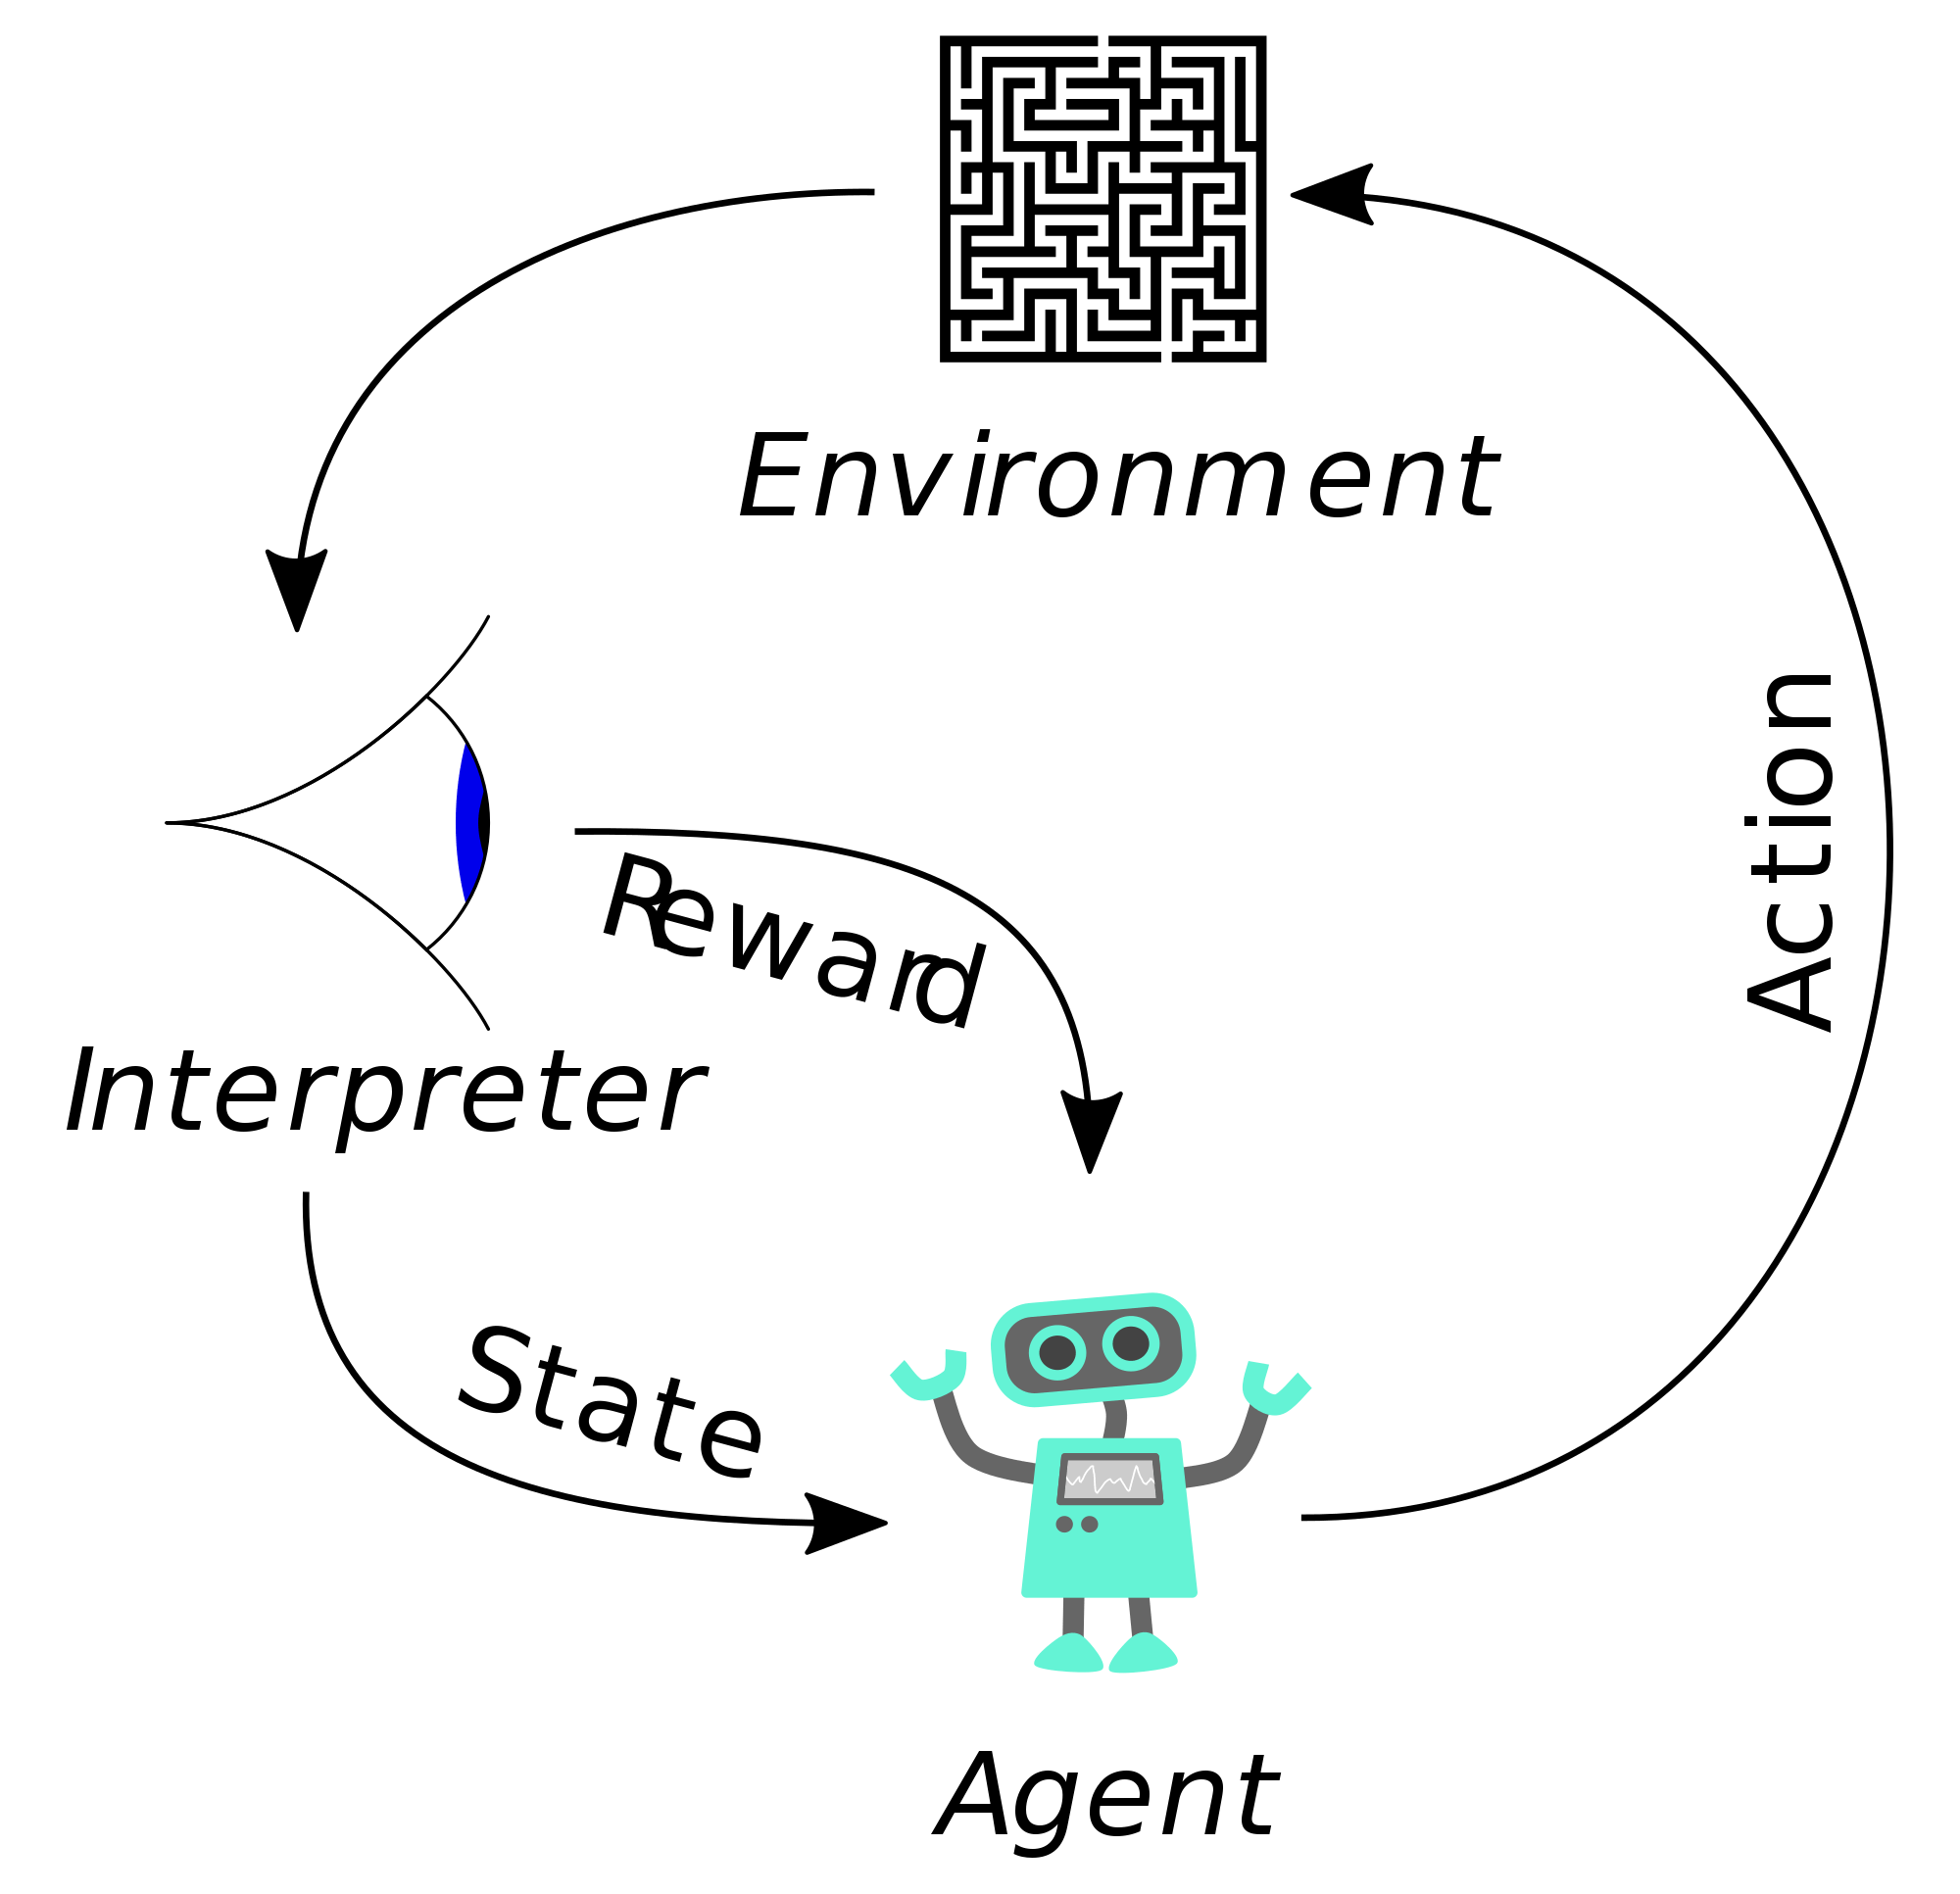
\includegraphics[scale=.1]{img/rl.png}
\end{center}
\end{minipage}
\caption[Reinforcement Learning problem scheme]{The scheme of a Reinforcement Learning model.}\label{F:rl}
\end{figure}

\subsection{Uncertainty in Reinforcement Learning}
The major challenge of Reinforcement Learning is represented by the uncertainty. In fact, initially, the agent is not provided with the knowledge of how the environment will react to its actions, thus it does not know whether an action would be good or not to maximize its objective function. In other words, before trying an action, it does not know if that action will get a positive or a negative reward, and it does not know if that action will let it go to the expected state or not. Thus, the former problem can be seen as uncertainty in the reward function and the latter as uncertainty in the transition (i.e. model) function. In some cases, also the uncertainty in the perception of the current state of the agent is considered, making the problem more complex.

The uncertainty issue results in the need of the agent to try actions in order to improve its knowledge of the environment. This process delays the collection of high rewards, but helps the agent to reduce its uncertainty. However, since the objective function is a sum of discounted rewards where later rewards worth less than recent ones, the agent also needs to learn fast in order to learn to perform the most rewarding actions as soon as possible. The need to \textit{explore} to reduce uncertainty and the need to \textit{exploit} the actions believed to be good introduces an important problem known as \textit{exploration-exploitation dilemma}.

\subsection{Balancing exploration and exploitation}
The exploration-exploitation dilemma has been broadly studied in the field of \gls{mab}, a particular case of the \gls{rl} problem with a single state~\cite{lai1985asymptotically}. In this problem the goal is to find the sequence of optimal actions, i.e. the sequence of actions that allows to maximize the return. The simplistic setting of the \gls{mab} problem allows to theoretically study the balancing of exploratory and exploitative actions, for instance to derive upper confidence bounds on the \textit{regret}, i.e. a measure of the return lost in performing non-optimal actions~\cite{bubeck2012regret, agrawal2012analysis, vermorel2005multi}, and several algorithms to address this problem have been proposed such as UCB1~\cite{auer2002finite} and Thompson Sampling~\cite{thompson1933likelihood}.

The \gls{rl} setting complicates the \gls{mab} problem because of the presence of multiple states. This makes the exploration-exploitation dilemma less tractable in terms of complexity and computational feasibility. Indeed, the quality of the actions must now be evaluated for each state, contrarily to the \gls{mab} case where the presence of a single state simplifies the problem. This issue is what makes \gls{rl} so challenging and has been addressed for decades in the literature.

\section{My research}
The strong connection between uncertainty and the exploration-exploitation dilemma is highlighted by the previous considerations and it is intuitive how the effectiveness of a \gls{rl} algorithm depends on its ability of reducing the uncertainty of the agent in a computationally and data-efficient way. The \gls{rl} literature contains lots of algorithms and methodologies proposed to make the agent learn a good policy aiming at efficiency; however, despite addressing the reduction of uncertainty via experience, only few of them explicitly exploit uncertainty to learn.

\subsection{What is my research about}
During my Ph.D., I studied ways to develop algorithms that exploit uncertainty since the explicit consideration of it has been shown to be often helpful to improve the performance and efficiency of learning. One of the most common technique to explore is known as $\varepsilon$-greedy and consists in performing, at each state, a random action with probability $\varepsilon$ and the action considered to be the best one with probability $1 - \varepsilon$. This exploratory policy does not consider the uncertainty of the agent and simply randomly moves it with the drawback of requiring a huge amount of experience to learn effective policies. This is shown especially in recent works on the field of \gls{drl}~\cite{mnih2015human, van2016deep, wang2015dueling} which studies the application of \gls{dl}~\cite{lecun2015deep} models and methodologies to exploit their strong ability to generalize with the purpose to solve highly complex problems that were unfeasible before. Research on \gls{drl}, brought to the realization of groundbreaking works where authors have been able to reach the state-of-the-art in extremely complex games such as Go~\cite{silver2016mastering, silver2017mastering} and chess~\cite{silver2017chess}.
However, the extraordinariness of these results is comparable to the amount of experience required by these algorithms to work. For instance, in~\cite{mnih2015human} the experiments are performed using $50^6$ samples corresponding to three days of computation and several weeks of human play. This work does not address the problem of data-efficiency aiming more to other goals (e.g. maximizing the cumulative reward) and for this reason the previously described exploration policy of $\varepsilon$-greedy is used.

\subsection{What I have done}
My Ph.D. research brought to the publication of four conference papers, most of them focused on the previously described topic. I also developed, together with a colleague of mine, a \gls{rl} Python library called \textit{Mushroom} which had the initial purpose to facilitate my research, but which has become larger and larger allowing now to do \gls{rl} research for general purposes. Details about Mushroom are reported in Appendix~\ref{App:msh}. Other works are still ongoing and others have not been accepted for publications yet, still I think they worth to be mentioned in this thesis anyway. The whole document is divided in four parts, with this introduction included in the first one:
\begin{itemize}
 \item \textbf{first} part includes this chapter and Chapter~\ref{C:soa} which introduces the main concepts of \gls{rl} starting from the fundamental theory and then giving a description of several methodologies related to this thesis with the purpose to provide a general, but useful, overview of what is necessary to understand the following chapters;
 \item \textbf{second} part includes the description of three publications I made about ways to exploit uncertainty in the context of value-based \gls{rl} and more in particular in the famous algorithm of $Q$-Learning. In particular, Chapter~\ref{C:mev} describes a novel way to address the problem of overestimation of the Maximum Expected Value in $Q$-Learning and Chapter~\ref{C:rq} describes a novel way to deal with uncertainty in the estimate of the components of the Bellman Operator;
 \item \textbf{third} part includes two works about the exploitation of uncertainty to drive exploration. Chapter~\ref{C:ts} describes a set of algorithms for the estimate of uncertainty of action-values to allow the use of an exploration policy inspired by Thompson Sampling. Chapter~\ref{C:opt} introduces a variant of the Bellman Operator which incorporates an optimistic update of the action-value estimate in order to favor exploration according to the principle of Optimism in the Face of Uncertainty;
 \item \textbf{fourth} and last part concludes the thesis resuming the previous chapters and giving my considerations about the research I made and the one I think will be interesting to pursue in the following years, by me or someone else!
\end{itemize}
 % uncomment if you want part I
\chapter{Preliminaries}\label{C:soa}
\gls{rl} is intuitively describable as the process of learning from interaction with the environment. This hasty explanation offers a very high level definition of it, then a more formal way to model the problem is required to properly analyze it. To this end, this chapter provides a description of the mathematical framework required to model \gls{rl}. It also explains a selection of algorithms that are related to the work done in this thesis in order to provide enough knowledge about the literature I dealt with during my years of Ph.D. research.

\section{Agent and environment}
\begin{figure}[b]
\begin{minipage}{\textwidth}
\begin{center}
  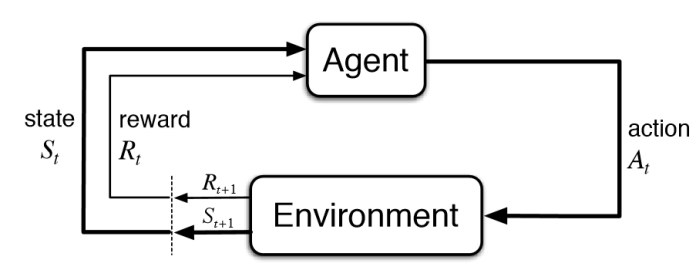
\includegraphics[scale=.75]{img/mdp1.jpg}
\end{center}
\end{minipage}
\caption[Scheme of a Markov Decision Process]{Graphical representation of a Markov Decision Process.}\label{F:mdp1}
\end{figure}
The interaction of an agent inside an environment can be seen as the execution of actions to move itself and the observation of the consequences of its actions (Figure \ref{F:mdp1}). The temporal progress of the interaction is modeled in a set of discrete time steps $t \in [0, 1, 2, \dots]$ where the agent sees a representation $s$ of the environment, executes an action $a$ and observes the new representation of the environment $s'$. The problems about observation and interaction discussed in Chapter~\ref{C:intro} are simplified by an explicit selection of data to observe from the environment and of the executable actions. In this way, only the relevant aspects of the sensory data acquired from the environment by the agent are used. The total number of time steps $t_i$ is called \textit{horizon} $H$ and determines a first taxonomy of problems:
\begin{itemize}
 \item finite time horizon: $t_i, \forall i \in [0, 1, 2, \dots, H)$;
 \item infinite time horizon: $t_i, \forall i \in [0, 1, 2, \dots, \infty)$.
\end{itemize}
Some problems can terminate before reaching the horizon, which happens when the agent reaches special situations called \textit{absorbing} states. These states are usually desired or catastrophic states when the interaction of the agent with the environment is no more useful or impossible. The set of steps between the start of the interaction to the end is called \textit{episode}.

The interaction of the agent with the environment is performed with the purpose to reach a goal for which the agent has been designed. The way to give the knowledge of the goal to the agent is to provide it with a measure of the quality of its behavior. This measure is called \textit{reward} $R(s,a,s')$ and is a function usually returning a real scalar value $r$ given the action $a$ performed by the agent in state $s$ and bringing to state $s'$. The goal of the agent is to maximize a measure related to the collected rewards. In an infinite time horizon problem it can be:
\begin{itemize}
 \item cumulative reward:
 \begin{equation}\label{E:sumrew}
  J = \sum_{t=0}^\infty r_t;
 \end{equation}
\item average reward:
\begin{equation}
 J = \lim_{n\to\infty}\dfrac{\sum_{t=0}^n r_t}{n};
\end{equation}
\item discounted cumulative reward:
\begin{equation}\label{E:discumrew}
 J = \sum_{t=0}^\infty \gamma^t r_t.
\end{equation}
\end{itemize}
The measure in Equation~\ref{E:discumrew} uses a real scalar $\gamma \in (0, 1]$, called \textit{discount factor}, which has the purpose to give different importance to rewards w.r.t. the time step they have been collected. If $\gamma = 1$ the equation reduces to~\ref{E:sumrew}, whereas the smaller it becomes the less the agent cares about rewards far in time.

\section{Markov Decision Processes}
\begin{figure}[t]
\begin{minipage}{\textwidth}
\begin{center}
  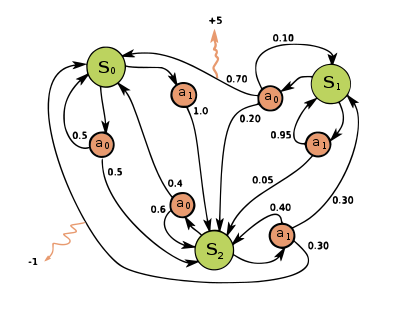
\includegraphics[scale=.6]{img/mdp2.png}
\end{center}
\end{minipage}
\caption[Example of a Markov Decision Process]{An example of a \gls{mdp} graph representing states $S_i$, actions $a_i$, transition probabilities (numbers over each edge) and rewards (pink arrows).}\label{F:mdp2}
\end{figure}
The mathematical framework to study the interaction of the agent with the environment is provided by the theory behind \glspl{mdp}. A \gls{mdp} is defined as a $6$-tuple where $\langle \mathcal{S}, \mathcal{A}, \mathcal{R}, \mathcal{T}, \gamma, \mu \rangle$:
\begin{itemize}
 \item $\mathcal{S}$ is the set of states where the agent can be in the environment;
 \item $\mathcal{A}$ is the set of actions that the agent can execute in the environment;
 \item $\mathcal{R}$ is the set of rewards obtainable by the agent;
 \item $\mathcal{T}$ is the \textit{transition function} consisting in the probability of reaching a state $s'$ executing action $a$ in state $s$: $\mathcal{T}(s, a) = P(s' | s, a)$;
 \item $\gamma$ is the discount factor;
 \item $\mu$ is the probability of each state to be the initial one: $\mu(s) = P(s_0 = s)$.
\end{itemize}
A \gls{mdp} is called \textit{finite}, or \textit{discrete}, if the set of states $\mathcal{S}$ and set of actions $\mathcal{A}$ are finite; it is called \textit{infinite}, or \textit{continuous}, when the set of states $\mathcal{S}$ is infinite and/or the set of actions $\mathcal{A}$ is infinite.
Two important properties of \glspl{mdp} are:
\begin{itemize}
 \item \textbf{stationarity:} the transition function $\mathcal{T}$ does not change over time;
 \item \textbf{Markovian assumption:} the transition and reward functions depend only on the current time step and not on the previous ones;
 \item \textbf{ergodicity:} a \gls{mdp} is called \textit{ergodic} when the agent can reach all the states of the \gls{mdp} from every state.
\end{itemize}
These three properties are taken as assumptions by most of the literature about \glspl{mdp} and by the works presented in this thesis too.

\subsection{Value functions}
Recalling that the goal of the agent is to maximize the cumulative (discounted) reward $J$ obtained during an episode, a \gls{mdp} is considered \textit{solved} when the agent learns the actions to perform in each state which maximizes this measure. The function defining the probability of executing action $a$ in a state $s$ is called \textit{policy}: $\pi(s) = P(a|s)$. An \textit{optimal} policy $\pi^*$ is the one which, when followed, allows the agent to solve the \gls{mdp}. Considering the stochasticity in the transition function $\mathcal{T}$ and in the policy $\pi$, the expected value of the cumulative discounted reward obtainable following $\pi$ is called \textit{state-value function}
\begin{equation}
 V_\pi(s) = \mathbb{E}_\pi[\sum_{k=0} \gamma^k r_{t+k}], \forall s \in \mathcal{S}.
\end{equation}
Then, an optimal policy can be defined also as the one which maximizes the value function of each state
\begin{equation}
 V^*(s) = \max_\pi V_\pi(s), \forall s \in \mathcal{S}.
\end{equation}
Together with the state-value function, the \textit{action-value function} is defined as
\begin{equation}
 Q_\pi(s, a) = \mathbb{E}_\pi[\sum_{k=0} \gamma^k r_{t+k}], \forall s \in \mathcal{S}, a \in \mathcal{A}.
\end{equation}
And subsequently the optimal policy maximizes also the action value function of each state-action tuple
\begin{equation}
 Q^*(s,a) = \max_\pi Q_\pi(s,a), \forall s \in \mathcal{S}, a \in \mathcal{A}.
\end{equation}

\section{Solving a MDP}
Value functions are the main concept used by several algorithms to address the problem of solving \glspl{mdp}. In the following, a description of algorithms exploiting value functions to solve \glspl{mdp} is provided, from the easiest case to the hardest ones.

\subsection{Dynamic Programming}
When the transition function $\mathcal{T}$ and reward function $\mathcal{R}$ of a \gls{mdp} are known, the full model of the environment is available. This is not the case in many real world problems where an agent does not know where the action would bring it and which return would obtain, but constitutes an interesting scenario to start studying the problem of solving a \gls{mdp}. The theory behind the solving of \glspl{mdp} with full model available is known under the name of \gls{dp}~\cite{bertsekas2005dynamic, bellman2013dynamic}. The main concept in the research on \gls{dp} is the optimal \gls{be}, defined as
\begin{align}
 V^*(s) &= \max_a \mathbb{E}[r_t + \gamma V^*(s')]\nonumber\\
        &= \max_a \sum_{s'} p(s' | s, a)[r + \gamma V^*(s')]
\end{align}
for state-value function, and
\begin{align}
 Q^*(s,a) &= \mathbb{E}[r_t + \gamma \max_{a'}Q^*(s', a')]\nonumber\\
          &= \sum_{s'} p(s' | s, a)[r + \gamma \max_{a'}Q^*(s', a')]
\end{align}
for action-value function $\forall (s, s') \in \mathcal{S} \times \mathcal{S}$ and $a \in \mathcal{A}$.
The optimal \gls{be} serves as a way to derive the optimal policy, but requires the optimal value functions to be known. Usually the optimal value functions are unknown and in order to learn them several algorithms change the \gls{be} in form of an assignment repeated iteratively.

\subsubsection{Policy Iteration}
The iterative application of the \gls{be} when following a policy $\pi$ is called \textit{iterative policy evaluation} (Algorithm~\ref{A:peval}) since it allows to compute the value functions of states and actions w.r.t. the policy $\pi$:
\begin{align}
 V_{t+1} (s) &= \mathbb{E}_\pi[r_t + \gamma V_t(s_{t+1})]\nonumber\\
             &= \sum_a \pi(a|s) \sum_s P(s' | s, a)[r + \gamma V_t(s')], \forall s \in \mathcal{S}. 
\end{align}
\begin{algorithm}[t]
 \caption{Iterative Policy Evaluation}
 \begin{algorithmic}[1]\label{A:peval}
  \STATE \textbf{Inputs:} policy $\pi$ to evaluate, a small threshold $\theta$ determining the accuracy of the estimate
  \STATE \textbf{Initialize:} $V(s), \forall s \in \mathcal{S}$ arbitrarily, $V(s') = 0$ for all terminal states $s'$
  \REPEAT
  \STATE $\Delta \gets 0$
  \FORALL{$s \in \mathcal{S}$}
  \STATE $v \gets V(s)$
  \STATE $V(s) \gets \sum_a \pi(a|s) \sum_{s'} P(s'|s,a)[r + \gamma V(s')]$
  \STATE $\Delta \gets \max(\Delta, |v - V(s)|)$
  \ENDFOR
  \UNTIL{$\Delta < \theta$}
 \end{algorithmic}
\end{algorithm}
It can be shown that the iterative application of the \gls{be} always converges to a single fixed point $V_\pi$.

Once the value functions have converged, it is interesting to see if the current policy $\pi$ can be improved in order to make it closer to the optimal one $\pi^*$ or not. One way to do this consists in considering a state $s$ and an action $a \neq \pi(s)$ and computing
\begin{align}
 Q_\pi(s,a) &= \mathbb{E}[r_t + \gamma V_\pi(s_{t+1})]\nonumber\\
            &= \sum_{s'} P(s' | s,a)[r + \gamma V_\pi(s')], \forall s \in \mathcal{S}, a \in \mathcal{A}.
\end{align}
Whenever $Q_\pi(s,a) > Q_\pi(s, \pi(s))$ it is convenient to update the policy such that $\pi(s) = a$. This procedure is called \textit{policy improvement}.
The process of alternating steps of iterative policy evaluation and policy improvement brings to the estimation of the optimal value functions and is resumed in an algorithm called \gls{pi} (Algorithm~\ref{A:piter}).
\begin{algorithm}[t]
 \caption{Policy Iteration}
 \begin{algorithmic}[1]\label{A:piter}
  \STATE \textbf{Initialize:} $\pi(s) \in \mathcal{A}$ arbitrarily for all $s \in \mathcal{S}$
  \REPEAT
  \STATE \textbf{Iteration policy evaluation}
  \STATE \textbf{Policy improvement:}
  \STATE $policy\_stable \gets true$
  \FORALL{$s \in \mathcal{S}$}
  \STATE $old\_a \gets \pi(s)$
  \STATE $\pi(s) \gets arg\max_a \sum_{s'} P(s'|s,a)[r + \gamma V(s')]$
  \STATE If $old\_a \neq \pi(s)$, then $policy\_stable \gets false$
  \ENDFOR
  \UNTIL{policy-stable}
 \end{algorithmic}
\end{algorithm}

\begin{algorithm}[t]
 \caption{Value Iteration}
 \begin{algorithmic}[1]\label{A:viter}
  \STATE \textbf{Inputs:} a small threshold $\theta$ determining the accuracy of the estimate
  \STATE \textbf{Initialize:} $V(s), \forall s \in \mathcal{S}$ arbitrarily, $V(s') = 0$ for all terminal states $s'$
  \REPEAT
  \STATE $\Delta \to 0$
  \FORALL{$s \in \mathcal{S}$}
  \STATE $v \to V(s)$
  \STATE $V(s) \to \max_{a} P(s'|s,a)[r + \gamma V(s')]$
  \STATE $\Delta \gets \max(\Delta, |v - V(s)|)$
  \ENDFOR
  \UNTIL{$\Delta < \theta$}
 \end{algorithmic}
\end{algorithm}

\subsubsection{Value Iteration}
The alternation of policy evaluation and policy improvement is a drawback of \gls{pi} which may slowdown the learning. Among other algorithms, the algorithm of \gls{vi} (Algorithm~\ref{A:viter}) addresses this problem stopping policy evaluation after only one update of each state value function. The update is different from the one in policy evaluation since it combines the policy evaluation steps and the policy improvement:
\begin{align}
 V_{t+1} (s) &= \max_a \mathbb{E}[r_t + \gamma V_t(s_{t+1})]\nonumber\\
             &= \max_a \sum_s P(s' | s, a)[r + \gamma V_t(s')], \forall s \in \mathcal{S}. 
\end{align}
Desirably, \gls{vi} maintains the properties of \gls{pi} about convergence to the fixed point corresponding to the optimal value functions.

As stated at the beginning of the section, the previous methods can be applied only when the full model of the \gls{mdp} is known. However, in most of real cases the full model is not available and the agent must move in the environment in order to understand it.

\subsection{Reinforcement Learning}
The purpose of \gls{rl} is to address the problem of solving a \gls{mdp} in the cases where \gls{dp} is not helpful, i.e. when the transition function $\mathcal{T}$ and reward function $\mathcal{R}$ are not known. To achieve this, the agent should acquire the necessary knowledge from transition samples obtained moving in the environment. There are two main ways of using the transition samples resulting in two classes of \gls{rl} algorithms:
\begin{itemize}
 \item \textbf{model-based:} the samples are used to learn a model of the environment which is subsequently used to learn the policy;
 \item \textbf{model-free:} the samples are used to directly compute the policy, for instance by means of value function approximation.
\end{itemize}
In both classes of methods, the \gls{rl} problem can be addressed in two ways:
\begin{itemize}
 \item \textbf{value-based:} the algorithm computes an estimate of the action-value function;
 \item \textbf{policy-based:} the algorithm computes an estimate of the policy.
\end{itemize}
This taxonomy splits the \gls{rl} literature in two sharply different fields where value-based is mostly used for discrete \glspl{mdp} whilst policy-based is mostly used in continuous \glspl{mdp}, in particular in Robotics~\cite{kober2013reinforcement}.

In all these classes of problems the policy followed to collect samples plays a crucial role since the performance of the learning algorithm heavily depends on the balancing between exploratory actions and exploitative actions, a fundamental issue of \gls{rl} known as \textit{exploration-exploitation dilemma}. The work done in this thesis is mainly focused on model-free value-based \gls{rl} in \gls{mdp} with a finite number of actions, thus all the following analysis is only inherent to it.

\paragraph{Exploration policies}
In a hypothetical setting in which the agent is provided the knowledge of the optimal policy $\pi^*$, there is no need to explore new actions and it can simply follow the optimal policy to solve the \gls{mdp} even without learning anything. Besides this very unlikely case, there are numerous situations where the agent does not know the environment it is moving in and the effect of its actions on the environment, then it needs to explore the environment to acquire the knowledge it needs to learn an optimal policy. The most trivial exploratory policy is called $\varepsilon$-greedy and is computed as
\begin{equation}\label{E:eps}
\pi(a|s)=
    \begin{cases}
    \dfrac{\varepsilon}{|\mathcal{A}|} + 1 - \varepsilon & \text{if } a = \arg\max_{a \in \mathcal{A}}Q(s,a)\\
    \dfrac{\varepsilon}{|\mathcal{A}|} & \text{otherwise}
    \end{cases}
\end{equation}
Equation~\ref{E:eps} results in choosing, at each step, between a greedy or a random action according to the value of $\varepsilon$: the policy is completely random when $\varepsilon = 1$ and is completely greedy when $\varepsilon = 0$.
Despite its simplicity, this policy is used in numerous works in literature allowing to reach good results with minimum computational demand, but at the cost of a bad sample-efficiency.

One of the drawbacks of $\varepsilon$-greedy is that it makes no use of the information available to the agent. The \textit{Boltzmann} policy, also known as \textit{Softmax} policy, makes use of the current estimate of the action-value functions computing the probabilities for each action $a_i$ to be sampled as
\begin{equation}\label{E:boltz}
 \pi(a | s) = \dfrac{e^{\nicefrac{Q(s,a)}{\tau}}}{\sum_{a' \in \mathcal{A}}e^{\nicefrac{Q(s,a')}{\tau}}}
\end{equation}
where $\tau$ is called \textit{temperature} and controls the exploration ratio such as if $\tau \to 0$ the policy is greedy and if $\tau \to \infty$ the policy is random. This is an attempt to use knowledge acquired by the agent in order to drive exploration in a smarter way than $\varepsilon$-greedy. A more recent strategy based on Boltzmann policy exploits the \gls{mm} operator to compute the Maximum Entropy \gls{mm} policy~\cite{asadi2016alternative}
\begin{equation}
 \pi(a | s) = \dfrac{e^{\nicefrac{Q(s,a)}{\tau}}}{\sum_{a' \in \mathcal{A}}e^{\nicefrac{Q(s,a')}{\tau}}}
\end{equation}
where $\beta$ is a value for which
\begin{equation}
 \sum_{a \in \mathcal{A}} e^{\beta(Q(s,a) - mm_\omega Q(s))}(Q(s,a)-mm_\omega Q(s))=0
\end{equation}
and
\begin{equation}\label{E:mm}
 mm_\omega Q(s) = \dfrac{\log(\dfrac{\sum_{i=1}^{|\mathcal{A}|}e^{\omega Q(s,a_i)}}{|\mathcal{A}|})}{\omega}.
\end{equation}
The \gls{mm} operator~\ref{E:mm} is a softmax operator with the desirable property of differentiability of the Boltzmann operator~\ref{E:boltz}, but differently from the Boltzmann it is also a contractive operator, thus being an interesting operator for computing the target of the \gls{be}. 

\subsubsection{Temporal Difference Learning}
Given a policy, \gls{rl} is able to evaluate it from raw experience differently from \gls{dp} which needs to know the complete model of the \gls{mdp}. A well-known class of methods to do this is called \gls{mc}~\cite{robert2013monte} and consists in collecting samples for an entire episode and then updating the considered value functions using the discounted cumulative reward obtained during the run:
\begin{equation}\label{E:mc}
 V(s) \gets V(s) + \alpha [G - V(s)]
\end{equation}
where $G$ is the cumulative reward obtained from state $s$ till the end of the episode and $\alpha$ is the learning rate.
The drawback of these techniques is that they need the episode to be finished before updating the value function estimates slowing down the learning time.

To keep the desirable property of \gls{mc} of being able to estimate value functions from raw experience without losing the good property of \gls{dp} of being able to update the same estimates after each step (i.e. \textit{bootstrapping}), \gls{td} methods have been studied in the past literature and are still one of the most used methods in \gls{rl}. The simplest \gls{td} method is known as \gls{td}$(0)$ and updates the value function after each step with
\begin{equation}
 V(s) \gets V(s) + \alpha [r + \gamma V(s') - V(s)].
\end{equation}
The success of \gls{td} over \gls{dp} and \gls{mc} is motivated by this simple update formula since the algorithm is able to take the advantages of both techniques with guarantees of convergence to the optimal value function.

\gls{td} methods can be used for control if, instead of computing the state-value function, the action-value function is computed. This class of methods is split in two subclasses according to which policy is followed to compute the target of the \gls{td} update:
\begin{itemize}
 \item \textbf{on-policy:} following the policy which the agent is learning;
 \item \textbf{off-policy:} following another policy.
\end{itemize}

\paragraph{SARSA}\label{S:SARSA}
The SARSA algorithm is a well-known on-policy TD method for control. Being an on-policy control method, given a policy $\pi$ its purpose is to estimate the action-value function $Q_\pi(s,a)$ for each $(s,a)$ tuple via the update formula:
\begin{equation}
 Q(s,a) \gets Q(s,a) + \alpha [r + \gamma Q(s',a') - Q(s,a)]
\end{equation}
where $a' = \pi(s')$. Being a \gls{td}$(0)$ variant for control, the same convergence properties of \gls{td}$(0)$ apply for SARSA.
\paragraph{$Q$-Learning}\label{S:Q-Learning}
The corresponding off-policy \gls{td} algorithm for control w.r.t. SARSA is \gls{ql}~\cite{watkins1989learning}. Contrarily to SARSA, \gls{ql} directly approximates the optimal action-value functions using a different policy to compute the target of the \gls{td} update. In particular, \gls{ql} uses the greedy policy to compute the target, resulting in the update formula
\begin{equation}\label{eq:Q-formula}
 Q(s,a) \gets Q(s,a) + \alpha_t(s,a) \left(r + \gamma \max_{a'} Q(s',a') - Q(s,a)\right).
\end{equation}

According to the difference between on-policy and off-policy methods, SARSA and \gls{ql} are two algorithms that may behave very differently in some problems where the agent can reach some catastrophic states. For instance, if the desired goal state is close to other undesirable catastrophic states, SARSA will learn a policy which let the agent stay far from undesired state and reach the goal safely but slowly; while \gls{ql} will learn a policy moving close to undesired states, but reaching the goal faster than SARSA. Thus, SARSA is more suitable for real applications, e.g. in Robotics, where the cost of reaching catastrophic situations is very high and is better to be conservative in order not to damage the physical system; on the contrary, \gls{ql} is more suitable when the cost of reaching bad states is not high, e.g. simulations.

\paragraph{Fitted $Q$-Iteration}\label{S:FQI}
A well known \gls{td} batch variant of $Q$-Learning is the \gls{fqi} algorithm~\cite{ernst2005tree}. The idea of \gls{fqi} is to reformulate the \gls{rl} problem as a sequence of supervised learning problems. Given a set of samples $\mathcal{D} = \left\{\langle s_i, a_i, r_i, s'_i \rangle \right\}_{1\leq i\leq N}$ previously collected by the agent according to a given sampling strategy, at each iteration $t$, \gls{fqi} builds an approximation $\hat{Q}$ of the optimal $Q$-function by fitting a regression model on a bootstrapped sample set
\begin{equation}
 \mathcal{D}_t = \left\{ \langle (s_i,a_i), r_i + \gamma \max_{a'} \hat{Q}\left(s'_i, a'\right) \rangle\right\}_{1 \leq i \leq N}.
\end{equation}
Under some conditions, the algorithm is proved to converge to the optimal $Q^*$ in a finite number of steps. \gls{fqi} has been firstly presented using extra-trees regression~\cite{geurts2006extremely}, but has been proved to work well with other kind of regression, e.g. neural network in the \gls{nfqi} algorithm~\cite{riedmiller2005neural} or \gls{gp} regression~\cite{rasmussen2005gaussian} in the Weighted Fitted $Q$-Iteration algorithm~\cite{deramo2017maximum}.

\subsubsection{Deep Reinforcement Learning}
The groundbreaking works that revived the research on \gls{rl} in recent years are certainly the ones belonging to the \gls{drl} field which consists of the use of \gls{dl} methodologies to address the \gls{rl} problem in complex high-dimensional \glspl{mdp}. Indeed, the very large state and action spaces together with the high number of features represent an obstacle to the learning with shallow \gls{rl} techniques making them computationally impractical. The recent coming of powerful computational resources, in particular the use of \glspl{gpu} for training deep neural networks in \gls{dl}, allowed to overcome this issue favoring the use of powerful deep function approximators in \gls{rl}.

\paragraph{Deep $Q$-Network}\label{S:dqn}
\begin{figure}[t]
\begin{minipage}{\textwidth}
\begin{center}
  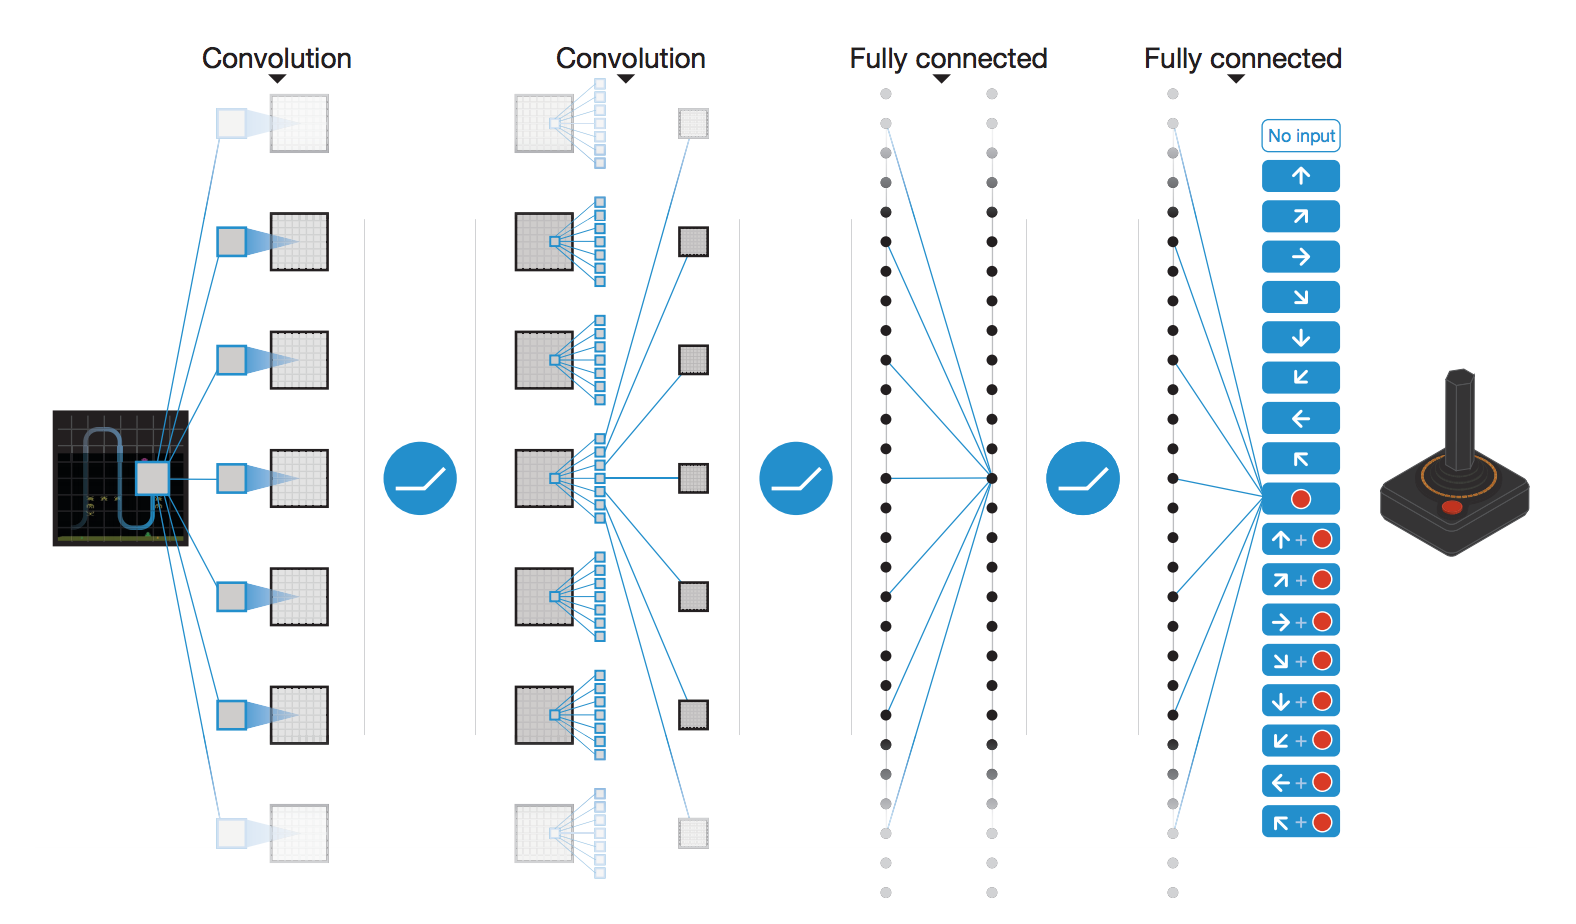
\includegraphics[scale=.19]{img/dqn.png}
\end{center}
\end{minipage}
\caption[DQN network scheme]{Synthetic scheme of a deep neural network which takes the input of the screen of a videogame and outputs the action to perform in that state.}
\end{figure}
The pioneering work which showed the potential of \gls{drl} and started the research about it is the \gls{dqn} algorithm~\cite{mnih2015human}. It consists in the use of a deep neural network and the storing of a replay memory of past transitions $\langle s_t, a_t, r_t, s'_t \rangle$ to approximate the action-value function $\hat{Q}$ of the problem computing the target
\begin{equation}\label{E:dqn_update}
y_i=
    \begin{cases}
    r_i & \text{if episode terminates at episode }i+1\\
    r_i + \gamma \max_{a'} \hat{Q}(s'_i, a') & \text{otherwise}
    \end{cases}
\end{equation}
and learning it in a supervised way.

The algorithm shows outstanding performance on the previously almost intractable problems of Atari games~\cite{bellemare2013arcade}, a set of more than $50$ old but challenging videogames, where \gls{dqn} achieves state-of-the-art results even beating a human expert in some of them. The most remarkable quality of \gls{dqn} is its relatively simple implementation consisting of using raw pixel frame as input of a convolutional network and applying a simple gradient descent step to update the network. In this way the complexity of the input, that made the solving of these problems intractable in the past, is addressed with the power of the deep convolutional network to extract highly abstract representation of it sensibly reducing its dimensionality and making it suitable for approximating the action-value function effectively. Despite its good properties, \gls{dqn} has some issues about sample-efficiency and the stability of learning that are common problems among \gls{drl} techniques. Indeed, the number of samples required by \gls{dqn} to learn are in the order of millions and corresponds to more than month of human playing; moreover in some games the algorithm shows very unstable performance even bringing to completely forgetting the good policy it learned after many steps. For these reasons, without forgetting the promising line of research that \gls{dqn} revealed, the following literature focused on many variants of \gls{dqn} to improve some of the issues it has. For instance, Double DQN~\cite{hasselt2015double} has been proposed to improve the estimate of the action-value function whereas Bootstrapped DQN~\cite{osband2017deep} aims to improve the exploration capabilities; both these algorithms will be considered and explained further in the thesis respectively in Chapter~\ref{C:mev} and~\ref{C:ts}.

\part{Bellman Update}
\chapter{Maximum Expected Value estimation}\label{C:mev}
\newcommand{\est}[1]{\hat\mu_*^{#1}}
\newcommand{\transpose}[1]{{#1}^\texttt{T}}

The computation of the \gls{mev} is required in several applications. Indeed, almost any process of acting involves the optimization of an expected utility function. For example, in the daily life decisions are usually made by considering the possible outcomes of each action based on partial information.
While sometimes only the order of preference of these alternatives matters, many applications require an explicit computation of the maximum utility.
For instance, in \gls{rl} the optimal policy can be found by taking, in each state, the action that attains the maximum expected cumulative reward. The optimal value of an action in a state, on its turn, depends on the \glspl{mev} of the actions available in the reached states.
Since errors propagate through all the state-action pairs, a bad estimator for the \gls{mev} negatively affects the speed of learning~\cite{van2010double}.

The most used approach to this estimation problem is the \gls{me} which simply takes the maximum estimated utility. As proved in~\cite{smith2006optimizer}, this estimate is positively biased and, if used in iterative algorithms, can increase the approximation error step-by step~\cite{van2010double}. More effective estimators have been proposed in the recent years. The \gls{de}~\cite{van2013estimating} approximates the maximum by splitting the sample set into two disjoint sample sets. One of this set is used to pick the element with the maximum approximate value and its value is picked from the other set. This has to be done the opposite way switching the role of the two sets. Eventually, the average (or a convex combination) of the two values is considered. This approach has been proven to have negative bias~\cite{van2013estimating} which, in some applications, allows to overcome the problem of \gls{me}.

During my years of Ph.D. research, we analyzed this problem and proposed the \gls{we}~\cite{deramo2016estimating} which approximates the maximum value by a sum of different values weighted by their probability of being the maximum. \gls{we} can have both negative and positive bias, but its bias always stays in the range between the \gls{me} and \gls{de} biases.

All the mentioned approaches are limited to a finite set of random variables, thus, in a subsequent work, we extended the study to problems with a set of infinite random variables and proposed an extension of \gls{we}~\cite{deramo2017maximum} to address them.

\section{Problem definition}
Given a finite set of $M \geq 2$ independent random variables $X = \lbrace X_{1}, ..., X_{M} \rbrace$, for each variable $X_i$ we denote with $f_i : \mathbb{R} \rightarrow \mathbb{R}$ its \gls{pdf}, with $F_i : \mathbb{R} \rightarrow \mathbb{R}$ its \gls{cdf}, with $\mu_i$ its mean, and with $\sigma^2_i$ its variance.
The \gls{mev} $\mu_{*}(X)$ is defined as
\begin{align}\label{E:maxExp}
\mu_{*}(X) = \max_{i} \mu_{i} = \max_{i} \int_{-\infty}^{+\infty}xf_i(x)~\mathrm{d}x.
\end{align}
Unfortunately, $\mu_{*}(X)$ cannot be found analytically if the \glspl{pdf} are unknown.
However it can be approximated using a given set of noisy samples $S = \lbrace S_{1}, ..., S_{N} \rbrace$ retrieved by the unknown distributions of each $X_{i}$ finding an accurate estimator $\est{}(S) \approx \mu_{*}(X)$. 
The random samples means $\hat{\mu}_{1}, ..., \hat{\mu}_{N}$ are unbiased estimators of the true means $\mu_{1}, ..., \mu_{N}$.
Eventually, the \gls{pdf} and \gls{cdf} of $\hat{\mu}_{i}(S)$ are denoted by $\hat f_i^S$ and $\hat F_i^S$.

\subsection{Related Works}
Several methods to estimate the \gls{mev} have been proposed in the literature. The most straightforward one is the \gls{me} which consists in approximating the \gls{mev} with the maximum of the sample means:
\begin{equation}\label{E:biasME}
\est{ME}(S) = \max_{i}\hat{\mu}_{i}(S) \approx \mu_{*}(X).
\end{equation}
Unfortunately, as proved in~\cite{smith2006optimizer}, this estimator has a positive bias that may cause issues in applications of \gls{me}, such as in the \gls{rl} algorithm of $Q$-Learning where the overestimation of the state-action values due to the positive bias can cause an error that increases step by step. However, the expected value of the \gls{me} is different from the \gls{mev} in~\ref{E:maxExp}. Consider the \gls{cdf} $\hat{F}_{\max}(x)$ of the \gls{me} $\max_{i}\hat\mu_{i}$ corresponding to the probability that \gls{me} is less than or equal to $x$. This probability is equal to the probability that all other estimates are less than or equal to $x$: 
$$\hat F_{\max}(x) = P(\max_{i}\hat\mu_{i} \leq x) = \prod^M_{i=1} P(\hat\mu_{i} \leq x) = \prod^M_{i=1} \hat F_i(x).$$
Considering the \gls{pdf} $\hat f_{\max}$, the expected value of the \gls{me} is $E\left[\est{ME}\right] = E [ \max_{i}\hat\mu_{i} ] = \int^{\infty}_{-\infty} x \hat f_{\max}(x) dx$. This is equal to
\begin{equation*}
E\left[\est{ME}\right] = \int^{\infty}_{-\infty} x \frac{d}{dx} \prod^M_{j=1} \hat F_j(x)~\mathrm{d}x =\sum^M_i \int^{\infty}_{-\infty} x \hat f_i(x) \prod^M_{i \neq j} \hat F_j(x)~\mathrm{d}x.
\end{equation*}
The presence of $x$ in the integral correlates with the monotonically increasing product $\prod^M_{i \neq j} \hat F_j(x)$ and causes the positive bias.

To solve this overestimation problem, a method called \gls{de} has been proposed in~\cite{van2010double} and theoretically analyzed in~\cite{van2013estimating}. \gls{de} uses a sample set $S$ retrieved by the true unknown distribution like \gls{me}, but splits it in two disjoint subsets $S^A = \lbrace S^A_{1}, ..., S^A_{N} \rbrace$ and $S^B = \lbrace S^B_{1}, ..., S^B_{N} \rbrace$. If the sets are split in a proper way, for instance randomly, the sample means $\hat{\mu}^A_{i}$ and $\hat{\mu}^B_{i}$ are unbiased, like the means $\hat{\mu}_{i}$ in the case of the \gls{me}. An estimator $a^*$, such that $\hat\mu^A_{a^*}(X) = \max_{i}\hat\mu^A_{i}(X)$, is used to pick an estimator $\hat\mu^B_{a^*}$ that is an estimate for $\max_{i}E [ \hat\mu^B_{i} ]$ and for $\max_{i}E [ X_{i} ]$. Obviously, this can be done the opposite way, using an estimator $b^*$ to retrieve the estimator value $\hat{\mu}^A_{b^*}$. 
\gls{de} takes the average of these two estimators.
The expected value of \gls{de} can be found in the same way as for \gls{me} with
\begin{equation}\label{E:biasCV}
E\left[\est{DE}\right]=\sum^M_i E \left[ \hat\mu^B_i \right] \int^{\infty}_{-\infty} \hat f^A_i(x) \prod^M_{j \neq i} \hat F^A_j(x)~\mathrm{d}x
\end{equation}
when using an estimator $a^*$ (the same holds by swapping A and B).
This formula can be seen as a weighted sum of the expected values of the random variables where the weights are the probabilities of each variable to be the maximum. Since these probabilities sum to one, the approximation given by \gls{de} results in a value that is lower than or equal to the maximal expected value. Even if the underestimation does not guarantee better estimation than the \gls{me}, it can be helpful to avoid an incremental approximation error in some learning problems. For instance, Double $Q$-Learning~\cite{van2010double} is a variation of $Q$-Learning that exploits this technique to avoid the previously described issues due to overestimation. Double $Q$-Learning has been tested in some very noisy environments and succeeded to find better policies than $Q$-Learning. Another remarkable application of \gls{de} is presented in~\cite{xu2013mab} where it achieves better results than \gls{me} in a sponsored search auction problem.

\section{Weighted Estimator}
Differently from \gls{me} and \gls{de} that output the sample average of the variable that is estimated to be the one with the largest mean, the proposed \gls{we} estimates the \gls{mev} $\mu_*(X)$ computing a weighted mean of all the sample averages:
\begin{equation}\label{E:WE}
\est{WE}(S) = \sum_{i=1}^M \hat\mu_i(S) w_i^S.
\end{equation}
Ideally, each weight $w_i^S$ should be the probability of $\hat\mu_i(S)$ being larger than all other samples means:  
$$w_i^S = P\left(\hat\mu_i(S) = \max_j \hat\mu_j(S)\right).$$
If we knew the \glspl{pdf} $\hat{f}_i^S$ for each $\hat\mu_i(S)$ we could compute the \gls{dwe}:
\begin{equation}\label{E:OptimalWE}
\est{DWE}(S) = \sum_{i=1}^M \hat\mu_i(S)\int_{-\infty}^{+\infty} \hat{f}_i^S(x) \prod_{j\neq i}\hat{F}_j^S(x)~\mathrm{d}x.
\end{equation}
We know that the sample mean $\hat\mu_i(S)$ is a random variable whose expected value is $\mu_i$ and whose variance is $\frac{\sigma^2_i}{|S_i|}$.
Unfortunately, its \gls{pdf} $\hat f_i^S$ depends on the \gls{pdf} $f_i$ of variable $X_i$ that is assumed to be unknown.
In particular, if $X_i$ is normally distributed, then, independently of the sample size, the sampling distribution of its sample mean is normal too: $\hat\mu_i(S)\sim\mathcal{N}\left(\mu_i,\frac{\sigma_i^2}{|S_i|}\right)$.
On the other hand, by the \gls{clt}, the sampling distribution $\hat f_i^S$ of the sample mean $\hat\mu_i(S)$ approaches the normal distribution as the number of samples $|S_i|$ increases, independently of the distribution of $X_i$.
Leveraging on these considerations, we propose to approximate the distribution of the sample mean $\hat\mu_i(S)$ with a normal distribution, where we replace the (unknown) population mean and variance of variable $X_i$ with their (unbiased) sample estimates $\hat\mu_i(S)$ and $\hat\sigma_i(S)$:
$$\hat f_i^S \approx \tilde f_i^S = \mathcal{N}\left(\hat\mu_i(S),\frac{\hat\sigma^2_i(S)}{|S_i|}\right),$$
so that \gls{we} is computed as:
\begin{equation}\label{E:WE2}
\est{WE}(S) = \sum_{i=1}^M \hat\mu_i(S)\int_{-\infty}^{+\infty} \tilde{f}_i^S(x) \prod_{j\neq i}\tilde{F}_j^S(x)~\mathrm{d}x.
\end{equation}

It is worth noting that \gls{we} is consistent with $\mu_*(X)$. In fact, as the number of samples grows to infinity, each sample mean $\hat\mu_i$ converges to the related population mean $\mu_i$, and the variance of the normal distribution $\tilde f_i$ tends to zero, so that the weights of the variables with expected value less than $\mu_*(X)$ go to zero, so that $\est{WE} \rightarrow \mu_*(X)$.

\subsection{Generalization to Infinite Random Variables}\label{S:infinite}
As far as we know, previous literature has focused only on the finite case and no approaches that natively handle continuous sets of random variables (e.g. without discretization) are available.
Let us consider a continuous space of random variables $\mathcal{Z}$ equipped with some metric (e.g. a Polish space) and assume that variables in $\mathcal{Z}$ have some spatial correlation.
Here, we consider $\mathcal{Z}$ to be a closed interval in $\mathbb{R}$ and that each variable $z \in \mathcal{Z}$ has unknown mean $\mu_z$ and variance $\sigma^2_z$.
Given a set of samples $S$ we assume to have an estimate $\hat{\mu}_z(S)$ of the expected value $\mu_z$ for any variable $z \in \mathcal{Z}$ (in the next section we will discuss the spatial assumption and we will explain how to obtain this estimate).
As a result, the weighted sum of equation~\ref{E:WE} generalizes to an integral over the space $\mathcal{Z}$:
\begin{align}\label{E:continuousWE}
\hat{\mu}_*^{\textrm{WE}}(S) = \int_{\mathcal{Z}} \hat{\mu}_z(S) \, 
\mathfrak{f}_z^*(S) \mathrm{d}z ,
\end{align}
where $\mathfrak{f}_z^*(S)$ 
is the probability density for $z$ of \emph{being the variable with the largest mean}, that plays the same role of the weights used in~\ref{E:WE}.
Given the distribution $f_{\hat{\mu}_z}^S$ of $\hat{\mu}_z(S)$, the computation of such density is similar to what is done in~\ref{E:WE2} for the computation of the weights $w_i^S$, with the major difference that in the continuous case we have to (ideally) consider a product of infinite cumulative distributions.
Let us provide a tractable formulation of such density function:

\begin{small}
\begin{align}
\nonumber \mathfrak{f}_z^*&(S) = f\left(\hat{\mu}_z(S) = \sup_{y \in \mathcal{Z}} \hat{\mu}_y(S)\right)\\
\nonumber &= \int_{-\infty}^{\infty}f(\hat{\mu}_z(S) = x) \; P \bigg( \hat{\mu}_y(S) \leq x, \; \forall y \in \mathcal{Z} \setminus \{z\} \bigg) \mathrm{d}x \\
\label{E:probability_events}
&= \int_{-\infty}^{\infty} f_{\hat{\mu}_z}^S(x) \; P \left( \bigwedge_{y \in \mathcal{Z} \setminus \{z\}} \hat{\mu}_y(S) \leq x \right) \mathrm{d}x \\
\label{E:probability_division}
&= \int_{-\infty}^{\infty} f_{\hat{\mu}_z}^S(x) \; \frac{P \left( \bigwedge_{y \in \mathcal{Z}} \hat{\mu}_y(S) \leq x \right)}{P \left( \hat{\mu}_{z}(S) \leq x \right)} \mathrm{d}x \\
\nonumber &= \int_{-\infty}^{\infty} f_{\hat{\mu}_z}^S(x) \; \frac{\Prodi_{\mathcal{Z}} F_{\hat{\mu}_y}^S(x)^{dy}}{F_{\hat{\mu}_z}^S(x)}\mathrm{d}x
\end{align}
\end{small}

\noindent where~\ref{E:probability_events}-\ref{E:probability_division} follow from the independence assumption.
The term $\prodi_{\mathcal{Z}} F^S_{\hat{\mu}_y}(x)^{dy} = P \left( \bigwedge_{y \in \mathcal{Z}} \hat{\mu}_y(S) \leq x \right)$ is the product integral defined in the geometric calculus (that is the generalization of the product operator to continuous supports) and can be related to the classical calculus through the following relation: $\Prodi_{\mathcal{Z}} F_{\hat{\mu}_y}^S(x)^{dy} = \exp{\left( \int_{\mathcal{Z}} \ln F_{\hat{\mu}_y}^S(x)dy \right)}$~\cite{grossman1972non}.

\subsubsection{Spatially Correlated Variables}
The issues that remain to be addressed are I) the computation of the empirical mean $\hat{\mu}_z(S)$ and II) the computation of the density function $f_{\hat{\mu}_z}^S$ (for each random variable $z \in \mathcal{Z}$).
In order to face the former issue we have assumed the random variables to be spatially correlated.
In this way we can use any regression technique to approximate the empirical means and generalize over poorly or unobserved regions.

In order to face the second issue, we need to restrict the regression class to methods for which it is possible to evaluate the uncertainty of the outcome.
Let $g$ be a generic regressor whose predictions are the mean of a variable $z$ and the \emph{confidence (variance) of the predicted mean} $\left(\text{i.e.}\; \hat{\mu}_z, \hat{\sigma}_{\hat{\mu}_z}^2 \leftarrow g(z) \right)$.
As done in the discrete case, we exploit the \gls{clt} to approximate the distribution of the sample mean $f_{\hat{\mu}_z}^S$ with a normal distribution $\tilde{f}_{\hat{\mu}_z}^S = \mathcal{N}\left(\hat{\mu}_z, \hat{\sigma}^2_{\hat{\mu}_z} \right)$.

As a result, the \gls{we} for the continuous case can be computed as follows:
% \begin{small}
\begin{align}\label{E:continuousWE2}
\hat{\mu}_*^{\textrm{WE}}(S) = \int_{\mathcal{Z}} \int_{-\infty}^{\infty}  \frac{\hat{\mu}_z(S)  \tilde{f}_{\hat{\mu}_z}^S(x)}{\tilde{F}_{\hat{\mu}_z}^S(x)} e^{\int_{\mathcal{Z}} \ln \tilde{F}_{\hat{\mu}_y}^S(x)\mathrm{d}y}\mathrm{d}x\mathrm{d}z.
\end{align}
% \end{small}
Since in the general case no closed-form solution exists for the above integrals, as in the finite case, the \gls{we} can be computed through numerical integration.

\subsubsection{Gaussian Process Regression}
While several regression techniques can be exploited (e.g. linear regression), the natural choice in this case is the \gls{gp} regression since it provides both an estimate of the process mean and variance.
Consider to have a \gls{gp} trained on a dataset of $N$ samples $\mathcal{D}=\{z_i, q_i\}_{i=1}^{N}$, where $q_i$ is a sample drawn from the distribution of $z_i$.
Our objective is to predict the target $q_*$ of an input variable $z_*$ such that $q_* = f(z_*) + \epsilon$ where $\epsilon \sim \mathcal{N}(0, \sigma_n^2)$.
Given a kernel function $k$ used to measure the covariance between two points $(z_i,z_j)$ and an estimate of the noise variance $\sigma^2_n$, the \gls{gp} approximation for a certain variable $z^*$ is $q_* \sim \mathcal{N}\left(\hat{\mu}_{z^*}, \hat{\sigma}^2_{\hat{\mu}_{z_*}} + \sigma_n^2\, I \right)$ where:
\begin{align}\label{E:gpmean}
\hat{\mu}_{z_*} &= \mathbf{k}^T_* \left(K + \sigma^2_n I\right)^{-1}\mathbf{q},\\
\nonumber
\hat{\sigma}^2_{\hat{\mu}_{z_*}} &= 
\text{Cov}\left(\mu_{z_*}\right) = k(z_*, z_*) - \transpose{\mathbf{k}}_* \left( K + \sigma^2_n I \right)^{-1}\mathbf{k}_*,
\end{align}
and $\mathbf{k}_*$ is the column vector of covariances between $z_*$ and all the input points in $\mathcal{D}$ ($\mathbf{k}_*^{(i)} = K(z_i, z_*)$), $K$ is the covariance matrix computed over the training inputs ($K^{(ij)} = k(z_i,z_j)$), and $\mathbf{q}$ is the vector of training targets.
Given the mean estimate in~\ref{E:gpmean}, the application of \gls{me} and \gls{de} is straightforward, while using \gls{we} requires to estimate also the \emph{variance of the mean estimates}.
The variance of the \gls{gp} target $q_*$ is composed by the variance of the mean ($\hat{\sigma}^2_{\hat{\mu}_{z_*}}$) and the variance of the noise ($\sigma^2_n$)~\cite{rasmussen2005gaussian}.
As a result, by only considering the mean contribute, we approximate the distribution of the sample mean by  $\tilde{f}_{\hat{\mu}_z}^S = \mathcal{N}\left(\hat{\mu}_z, \hat{\sigma}^2_{\hat{\mu}_z} \right)$ as defined in equations~\ref{E:gpmean}.

\section{Analysis of Weighted Estimator}
In this section, we theoretically analyze the estimation error of $\est{WE}(S)$ in terms of bias and variance, comparing it with the results available for \gls{me} and \gls{de}.
Although \gls{dwe} cannot be used in practice, we include it in the following analysis since it provides an upper limit to the accuracy of \gls{we}.

\subsection{Bias}

\begin{figure}
\centering
	\begin{minipage}{0.45\textwidth}
	\centering
	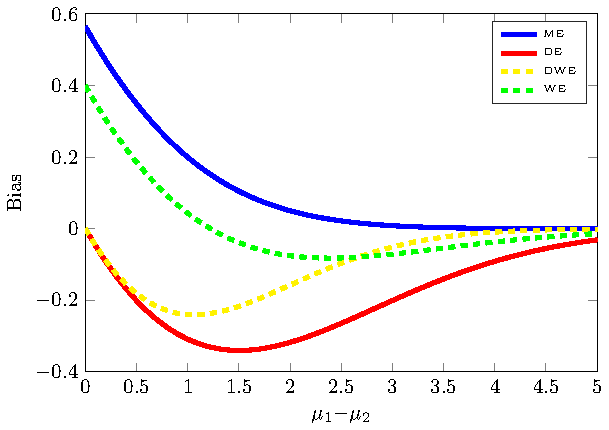
\includegraphics[scale=0.7]{./img/bias.pdf}
    \caption[Bias analysis in WE]{Comparison of the bias of the different estimators varying the difference of the means}\label{F:bias}
	\end{minipage}
	  \hfill
	\begin{minipage}{0.45\textwidth}
	\centering	
	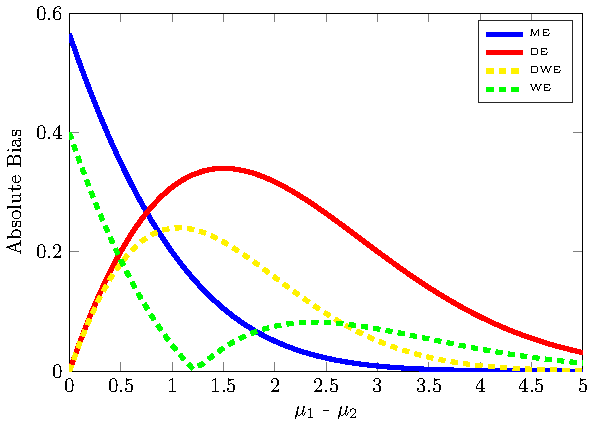
\includegraphics[scale=0.7]{./img/absolute_bias.pdf}
	\caption[Absolute bias analysis in WE]{Comparison of the absolute bias of the different estimators varying the difference of the means.}\label{F:absolute_bias}
	\end{minipage}
\end{figure}

We start with summarizing the main results about the bias of \gls{me} and \gls{de} reported in~\cite{van2013estimating}.
For what concerns the direction of the bias, \gls{me} is positively biased, while \gls{de} is negatively biased.
If we look at the absolute bias, there is no clear winner. 
For instance, when all the random variables are identically distributed, \gls{de} is unbiased, while the same setting represents a worst case for \gls{me}.
On the other hand, when the maximum expected value is sufficiently larger than the expected values of the other variables, the absolute bias of \gls{me} can be significantly smaller than the one of \gls{de}.
The bias of \gls{me} is bounded by:
$$\mathrm{Bias}\left(\est{ME}\right) \leq \sqrt{\frac{M-1}{M}\sum_{i=1}^M \frac{\sigma_i^2}{|S_i|}}.$$
For the bias of \gls{de}, \cite{van2013estimating} conjectures the following bound (which is proved for two variables):
$$\mathrm{Bias}\left(\est{DE}\right) \geq -\frac{1}{2}\left(\sqrt{\sum_{i=1}^M \frac{\sigma_i^2}{|S^A_i|}} + \sqrt{\sum_{i=1}^M \frac{\sigma_i^2}{|S^B_i|}}\right). $$

In the next theorem we provide a relationship between the bias of \gls{we} and the one of \gls{me}.
\begin{theorem}\label{T:BiasWEME}
 For any given set $X$ of $M$ random variables:
 $$\mathrm{Bias}(\est{WE}) \leq \mathrm{Bias}(\est{ME}) \leq \sqrt{\frac{M-1}{M}\sum_{i=1}^M \frac{\sigma_i^2}{|S_i|}}.$$
\end{theorem}
This does not mean that the absolute bias of \gls{we} is necessarily smaller than the one of \gls{me}, since (as we will see later) the bias of \gls{we} can be also negative.
In order to better characterize the bias of \gls{we}, we put it in relation with the bias of \gls{de}.
\begin{theorem}\label{T:BiasWECV}
 For any given set $X$ of $M$ random variables:
  $$\mathrm{Bias}(\est{WE}) \geq \mathrm{Bias}(\est{DE}).$$
\end{theorem}

\textbf{Example} In Figures~\ref{F:bias} and~\ref{F:absolute_bias} we visualize the bias of the different \gls{mev} estimators in a setting with two normally distributed random variables ($X_1\sim\mathcal{N}(\mu_1,\sigma_1^2)$ and $X_2\sim\mathcal{N}(\mu_2,\sigma_2^2)$) as a function of the difference of their expected values. Both variables have variance equal to 10 ($\sigma_1^2=\sigma_2^2=10$) and we assume to have 100 samples for each variable ($|S_1|=|S_2|=100$).
Figure~\ref{F:bias} confirms the previous theoretical analysis: the bias of \gls{me} is always positive, while the biases of \gls{dwe} and \gls{de} are always negative, with the latter always worse than the former.
The bias of \gls{we} can be positive or negative according to the situation, but it always falls in the range identified by the biases of \gls{me} and \gls{de}.
Looking at the absolute biases shown in Figure~\ref{F:absolute_bias}, we can notice that there is not a clear winner.
As previously mentioned, when the variables have the same mean, both \gls{de} and \gls{dwe} are unbiased, while it represents a worst case for the bias of \gls{me} and \gls{we}. It follows that, when the difference of the two means is small (less than 0.5 in the example), \gls{de} suffers less absolute bias than \gls{me} and \gls{we}. For moderate differences of the means (between 0.5 and 1.8 in the example), \gls{we} has the minimum absolute bias, while \gls{me} is preferable for larger differences.
Such results can be generalized as follows: \gls{de} suffers a small bias when there are several variables that have expected values close (w.r.t.~their variances) to the maximum one, while \gls{me} provides the best estimate when there is one variable whose expected value is significantly larger (w.r.t.~the variances) than all the expected values of all the other variables. In all the other cases, \gls{we} is less biased.

\subsection{Variance}
\begin{figure}
\centering
	\begin{minipage}{0.45\textwidth}
	\centering
	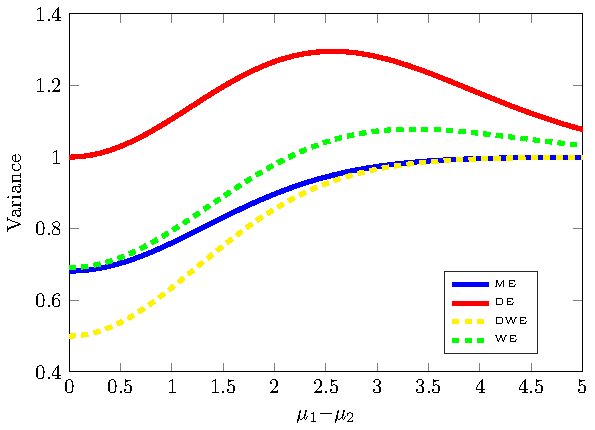
\includegraphics[scale=0.7]{./img/variance.pdf}
    \caption[Variance analysis in WE]{Comparison of the variance of the different estimators varying the difference of the means.}\label{F:variance}
	\end{minipage}
	  \hfill
	\begin{minipage}{0.45\textwidth}
	\centering	
	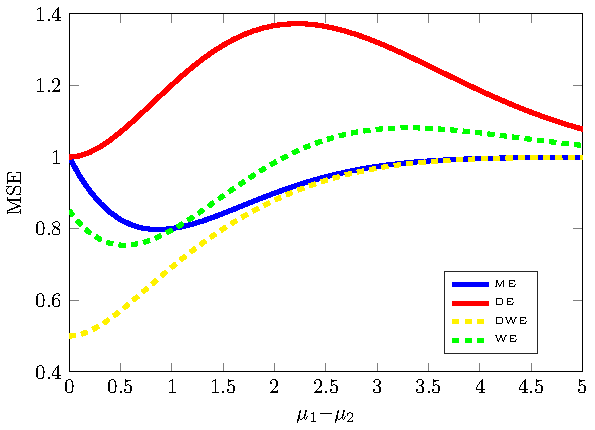
\includegraphics[scale=0.7]{./img/mse.pdf}
	\caption[MSE analysis in WE]{Comparison of the MSE of the different estimators varying the difference of the means.}\label{F:mse}
	\end{minipage}
	\label{F:Variance_mse}
\end{figure}

We cannot evaluate the goodness of an estimator by analyzing only its bias.
In fact, since the \gls{mse} of an estimator is the sum of its squared bias and its variance, we need to take into consideration also the latter.

\cite{van2013estimating} proved that both the variance of \gls{me} and the one of \gls{de} can be upper bounded with the sum of the variances of the sample means:
$ \mathrm{Var}\left(\est{ME}\right) \leq \sum_{i=1}^M \frac{\sigma^2_i}{|S_i|}$, $\mathrm{Var}\left(\est{DE}\right) \leq \sum_{i=1}^M \frac{\sigma^2_i}{|S_i|}$.
The next theorem shows that the same upper bound holds also for the variance of \gls{we}.
\begin{theorem}\label{T:VarianceWE}
 The variance of \gls{we} is upper bounded by
 $$\mathrm{Var}\left(\est{WE}\right) \leq \sum_{i=1}^M \frac{\sigma^2_i}{|S_i|}.$$
\end{theorem}
The bound in Theorem~\ref{T:VarianceWE} is overly pessimistic; in fact, even if each weight $w_i^S$ is correlated to the other weights and to the sample mean $\hat\mu_i(S)$, their sum is equal to one.
For sake of comparison, we upper bound the variance of \gls{dwe}.
\begin{theorem}\label{T:VarianceOWE}
 The variance of \gls{dwe} is upper bounded by
 $$\mathrm{Var}\left(\est{DWE}\right) \leq \max_{i\in{1,\dots,M}} \frac{\sigma^2_i}{|S_i|}.$$
\end{theorem}

\textbf{Example} As done for the bias, in Figure~\ref{F:variance} we show the variance of the different estimators under the same settings described above.
As the difference of the means of the two variables grows, the variance of all the estimators converges to the variance of the sample mean of the variable with the maximum expected value.
\gls{de} is the estimator with the largest variance since its sample means are computed using half the number of samples w.r.t.~the other estimators.
\gls{we} exhibits a variance slightly larger than the one of \gls{me}, while, as expected, the variance of \gls{dwe} is always the smallest.

Finally, in Figure~\ref{F:mse} we show the \gls{mse} $(variance + bias^2)$ of the different estimators.
When the difference between the two means is less than one, \gls{we} suffers from a lower \gls{mse} than the other two estimators.
On the other hand, \gls{me} is preferable when there is a variable with an expected value that is significantly larger than the other ones.

\section{Maximum Expected Value estimation in Reinforcement Learning}
Among value-based methods, we consider online and offline algorithms that approximate the optimal action-value function $Q^*$ without the need of a model of the environment. We consider mostly \glspl{mdp} with discrete action spaces, except for the batch algorithm based on \gls{we} that can be extended also to \glspl{mdp} with continuous action spaces.

\subsection{Online}
It is demonstrated that since $Q$-learning~\ref{S:Q-Learning} is a stochastic approximation algorithm, under the assumption that each state-action pair is visited infinitely often and the step sequence satisfies certain conditions, $Q_k$ converges to $Q^{*}$~\cite{watkins1989learning}. However, under particular conditions, such as a wrong tuning of parameters and noisy environments, the $Q$-function could converge to $Q^{*}$ too much slowly. One of the main reasons is that the $Q$-learning uses the \gls{me} to estimate the current maximum $Q$-value of the next state $s'$. Since this estimator is positively biased, and since the error is propagated at each step, the $Q$-function can be wrongly estimated and the algorithm could fail.
In the last years, different approaches have been proposed trying to overcome this issue~\cite{lee2013bias,bellemare2015increasing,ijcai2017-483}. In particular, the most successful one is the Double $Q$-Learning algorithm~\cite{van2010double} which replaces the \gls{me} used in $Q$-Learning with \gls{de}. The underestimation of the $Q$-function performed by Double $Q$-Learning allows to learn a good policy in very noisy environments where $Q$-Learning fails.

\begin{algorithm}[t]
\caption{Weighted Q-learning}
\label{A:WQ-Learning}
\begin{algorithmic}[1]
\STATE Initialize $Q(s,a) = 0$, $\mu(s,a) = 0$, $\sigma(s,a) = \infty$ and $s$
\REPEAT
\STATE $a \leftarrow$ drawn from policy $\pi(\cdot|s)$ (e.g., $\varepsilon$-greedy)
\STATE $s',r \leftarrow \text{MDP}(s,a)$
\STATE $\tilde{f}_m^S \leftarrow \mathcal{N}(\mu(s,a_m), \sigma^2(s,a_m))\quad \forall a_m \in \mathcal{A}$ 
\STATE $w_m \leftarrow \int_{-\infty}^{+\infty} \tilde{f}_m^S(x) \prod_{k\neq m} \tilde{F}^S_k(x) \mathrm{d}x \quad \forall a_m \in \mathcal{A}$
\STATE $W(s') \leftarrow \sum_{a_m \in \mathcal{A}} w_m Q(s',a_m)$
\STATE $Q(s,a) \leftarrow Q(s,a) + \alpha(s,a) (r + \gamma W(s') - Q(s,a))$
\STATE Update $\mu(s,a)$ and $\sigma(s,a)$ using tuple $\langle s,a,r \rangle$
\STATE $s \leftarrow s'$
\UNTIL {terminal condition}
\end{algorithmic}
\end{algorithm}

\subsubsection{Weighted Q-Learning}
We propose to replace \gls{me} with \gls{we} in the \textit{Weighted $Q$-Learning} algorithm~\cite{deramo2016estimating}. Weighted $Q$-Learning maintains an estimate of the mean value of the $Q$-function and its variance in order to compute the weights of \gls{we} (Algorithm \ref{A:WQ-Learning}).
While the mean value corresponds to the current estimate of the $Q$-function, the variance is not straightforward to be computed. Indeed, it is not simply the variance of the $Q$-function approximator, but it is the variance of the process consisting of an update formula with a variable learning rate. Considering this, it can be showed that the variance can be computed incrementally at each step $t$ with:
$$\sigma^2_t(s,a) \leftarrow n_t(s,a) \dfrac{(Q_{2_t}(s,a) - Q_t(s,a)^2)}{n_t(s,a) - 1} \omega_t(s,a),$$
where $Q_t(s,a)$ is the current $Q$-value of action $a$ in state $s$, $n_t(s,a)$ is the current number of updates of $Q(s,a)$ and
$$Q_{2_t}(s,a) = Q_{2_{t-1}}(s,a) + \dfrac{(r_t + \gamma W_t(s'))^2 - Q_{2_{t-1}}(s,a)}{n_t(s,a)},$$
$$\omega_t(s,a) \leftarrow (1 - \alpha_t(s,a))^2 \omega_{t-1}(s,a) + \alpha_t(s,a)^2$$
where $W_t(s')$ is the current value of \gls{we} in state $s'$.

\subsection{Batch}
The \gls{fqi} update~\ref{S:FQI}, similarly to the $Q$-Learning update, requires the computation of \gls{me} which causes the same overestimation problem of $Q$-Learning. Intuitively, the replacement of \gls{me} with \gls{de} or \gls{we} can help to solve this issue also in \gls{fqi}.

\begin{algorithm}[t]
\caption{Weighted FQI (finite actions)}
\label{A:WFQI}
\begin{small}
\begin{algorithmic} 
\STATE \textbf{Inputs:} dataset $\mathcal{D}=\{s_i,a_i,r_i,s'_i\}_{i=1}^{K}$, GP regressor $\widehat{Q}$, horizon $T \in \mathbb{N}$, discrete action space $\mathcal{A} = \{a_1,\ldots, a_M\}$
\STATE Train $\widehat{Q}_0^{\bar a}$ on $\mathcal{T}_0 = \{\langle s_i, r_i\rangle  \text{ s.t. } a_i = \bar{a} \}$ ($\forall \bar{a} \in \mathcal{A}$)
\FOR{t=1 \TO T}
\FOR{j=1 \TO K}
\FOR{m=1 \TO M}
\STATE $\hat{\mu}_{m}, \sigma^2_{\hat{\mu}_{m}} \leftarrow \widehat{Q}_{t-1}^{a_m}(s'_j)$ (evaluate GP)
\STATE $\tilde{f}_{\hat{\mu}_{m}}^S \leftarrow \mathcal{N}(\hat{\mu}_{m}, \sigma^2_{\hat{\mu}_m})$ ($\tilde{F}_{\hat{\mu}_{m}}^S$ is the associated CDF) 
\STATE $w_{a_m} \leftarrow \int_{-\infty}^{+\infty} \tilde{f}_{\hat{\mu}_{m}}^S(x) \prod_{k\neq m} \tilde{F}^S_{\hat{\mu}_{m}}(x) \mathrm{d}x$
\ENDFOR
\STATE $\mathcal{T}_t \leftarrow \mathcal{T}_t \cup \{(s_j,a_j), r_j + \gamma \sum_{a_m \in \mathcal{A}} w_{a_m} \mu_{a_m}\}$
\ENDFOR
\STATE Train $\widehat{Q}_t^{\bar a}$ on $\mathcal{T}_t = \{\langle s_i, r_i\rangle  \text{ s.t. } a_i = \bar{a} \}$ ($\forall \bar{a} \in \mathcal{A}$)
\ENDFOR
\end{algorithmic}
\end{small}
\end{algorithm}

\begin{algorithm}[t]
\caption{Weighted FQI$_{\infty}$ (continuous actions)}
\label{A:continuousWFQI}
\begin{small}
\begin{algorithmic} 
\STATE \textbf{Inputs:} dataset $\mathcal{D}=\{s_i,a_i,r_i,s'_i\}_{i=1}^{K}$, GP regressor $\widehat{Q}$, horizon $T \in \mathbb{N}$
\STATE Train $\widehat{Q}_0$ on $\mathcal{T}_0 = \{\langle (s_i, a_i), r_i\rangle \}$
\FOR{t=1 \TO T}
\FOR{i=1 \TO K}
\STATE $\hat{\mu}_{z}, \sigma^2_{\hat{\mu}_{z}} \leftarrow \widehat{Q}_{t-1}(s'_i, z)$ (evaluate GP)
\STATE $\tilde{f}_{\hat{\mu}_z}^S \leftarrow \mathcal{N}(\hat{\mu}_{z}, \sigma^2_{\hat{\mu}_z})$ ($\tilde{F}_{\hat{\mu}_z}^S$ is the associated CDF) 
\STATE $v_i \leftarrow \int_{-\infty}^{\infty} \exp{\left( \int_{\mathcal{Z}} \ln \tilde{F}_{\hat{\mu}_y}^S(x)\mathrm{d}y \right)} \int_{\mathcal{Z}}  \frac{\hat{\mu}_z(S)  \tilde{f}_{\hat{\mu}_z}^S(x)}{\tilde{F}_{\hat{\mu}_z}^S(x)} \mathrm{d}z\mathrm{d}x$
\STATE $\mathcal{T}_t \leftarrow \mathcal{T}_t \cup \{(s_i,a_i), r_i + \gamma v_i\}$
\ENDFOR
\STATE Train $\widehat{Q}_t$ on $\mathcal{T}_t$
\ENDFOR
\end{algorithmic}
\end{small}
\end{algorithm}

\subsubsection{Weighted Fitted Q-Iteration}
The \gls{fqi} variant which replaces \gls{me} with \gls{de} is called \gls{dfqi}, and the variant which we propose using \gls{we} is called \textit{Weighted} \gls{fqi} (WFQI)~\cite{deramo2017maximum}. \gls{wfqi} uses \gls{gp} regression in order to compute the mean $Q$-value and its variance in continuous state spaces (Algorithm \ref{A:WFQI}). The interesting aspect of \gls{wfqi} is that it can handle infinite action spaces too, as explained in Section \ref{S:infinite} and showed in Algorithm \ref{A:continuousWFQI}. At the best of our knowledge, this makes it the only value-based algorithm able to deal with infinite action spaces.

\subsection{Deep Reinforcement Learning}
We also analyzed the case of \gls{drl} where the overestimation problem caused by \gls{me} happens also in the \gls{dqn} algorithm resulting in critical loss of performance in some problems due to instability. The \gls{ddqn} algorithm~\cite{hasselt2015double} replaces \gls{me} with \gls{de} and shows considerable improvements and performance and stability. We worked on the replacement of \gls{me} with \gls{we} even though it is not straightforward in this case due to difficulties in computing the variance of the approximation. The \gls{gp} regression, used in \gls{wfqi}, is commonly not used in \gls{drl} and a deep neural network adapts better in important \gls{drl} problems, such as the well known Atari domain. The estimation of mean and variance with a neural network is possible, but the computational complexity increases with the number of parameters such that it becomes unfeasible in deep neural networks.

\subsubsection{Weighted Deep Q-Network}\label{S:drl}
\begin{figure}[t]
\begin{center}
  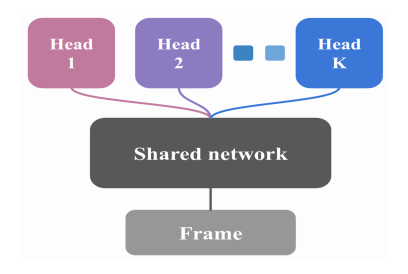
\includegraphics[scale=.5]{img/bdqn.png}
\end{center}
\caption[Boostrapped DQN network]{Architecture of the neural network used in Bootstrapped DQN.}\label{F:bdqn-net}
\end{figure}
We propose to estimate the variance of the approximation using an ensemble of target networks, following the neural network architecture proposed in another algorithm called \gls{bdqn}~\cite{osband2017deep} showed in Figure~\ref{F:bdqn-net}. This work follows the \gls{dqn} algorithm described in~\cite{mnih2015human} with few, but important changes. The output of the neural network is split in $K$ heads that share the same first hidden layers. To perform bootstrapping, a binary mask $w_1, \dots, w_K \in {0,1}$ is assigned to each sample to indicate the heads assigned to it. The binary mask is generated with a binomial distribution with probability $p$. The exploration policy of \gls{bdqn} uniformly samples a head at the beginning of the episode, and follow the greedy policy learned by it. During the learning phase, the different heads are updated following the update rule of \gls{ddqn} to avoid the overestimation problem.

We propose to use the architecture of \gls{bdqn} and use \gls{we} to compute the target of the $K$-th head, while using the target provided by \gls{me} for the other $K-1$ heads. Moreover, we only use the $K$-th head trained with \gls{we} for exploration. This way, the training of the $K-1$ heads do not differ from the one of \gls{bdqn}, while the $K$-th head is trained with \gls{we} exploiting the uncertainty on the action-values provided by the ensemble. Given a dataset of transitions $\langle s_t, a_t, r_t, s'_t \rangle$, the resulting formulas to compute the target $y^k$ of each head $k$ are:
\begin{equation}\label{E:dqn_update}
y_i^k=
    \begin{cases}
    r_i & \text{if episode terminates at episode }i+1\\
    r_i + \gamma \max_{a'} \hat{Q^k}(s'_i, a') & \text{otherwise}
    \end{cases}
\end{equation}
with $k \in \lbrace 1, \dots, K-1 \rbrace$ and
\begin{equation}\label{E:dqn_update}
y_i^K=
    \begin{cases}
    r_i & \text{if episode terminates at episode }i+1\\
    r_i + \gamma \sum_{j \in {1, \dots, \#\mathcal{A}}} w^j_i Q^K(s_i', a_j; \theta_K^-) & \text{otherwise}
    \end{cases}
\end{equation}
for the $K$-th head where $w^j_i$ is the percentage of the $K-1$ heads where action $a_j$ is the one with the highest action-value and $\theta_K^-$ are the parameters of the target network of the head $k$. To compute the action under the given policy, only the $K$-th head is used.
The resulting algorithm is a slight change to the original \gls{bdqn} that allows to use the \gls{we} in the \gls{dqn} framework without differences in computational time and memory requirements w.r.t. \gls{bdqn}. We call this algorithm \gls{wdqn}.

\section{Empirical results}
We evaluate the performance of \gls{me}, \gls{de} and \gls{we} in \gls{mab} and \gls{rl} problems. We start from considering discrete state and action spaces, then we move to continuous ones and, eventually, to deep \gls{rl} problems.

\subsection{Discrete States and Action Spaces}

\subsubsection{Internet Ads}
We consider this \gls{mab} problem as formulated in~\cite{van2013estimating}.
The goal in this problem is to select the most convenient ad to show on a website among a set of $M$ possible ads, each one with an unknown expected return per visitor. 
It is assumed that each ad has the same return per click, therefore the best ad is the one with the maximum \gls{ctr}.
Since the \glspl{ctr} are unknown, they have to be estimated from data.
In our setting, given $N$ visitors, each ad is shown the same number of times, so that we have $N/M$ samples to compute the sample \gls{ctr}.
It is desirable to obtain a quick and accurate estimate of the maximum \gls{ctr} in order to effectively determine future investment strategies.
We compare the results of \gls{me}, \gls{de} and \gls{we} in three different settings. 
We consider a default configuration where we have $N=300000$ visitors, $M = 30$ ads and mean \gls{ctr} uniformly sampled from the interval $[0.02,0.05]$.
In the first setting, we vary the number of visitors $N = \lbrace 30000, 60000, ..., 270000, 300000 \rbrace$, so that the number of impressions per ad ranges from $1000$ to $10000$.
In the second setting, we vary the number of ads $M = \lbrace 10, 20, ..., 90, 100 \rbrace$ and the number of visitors is set to $N=10000M$.
In the last setting, we modify the interval of the mean \gls{ctr} by changing the value of the upper limit with values in $\lbrace 0.02, 0.03, ..., 0.09, 0.1 \rbrace$, with the lower fixed at $0.02$.

\begin{figure*}[t]
    \begin{minipage}{\textwidth}
    \centering
    \subfigure[Increasing number of impressions.\label{F:ia_first}]{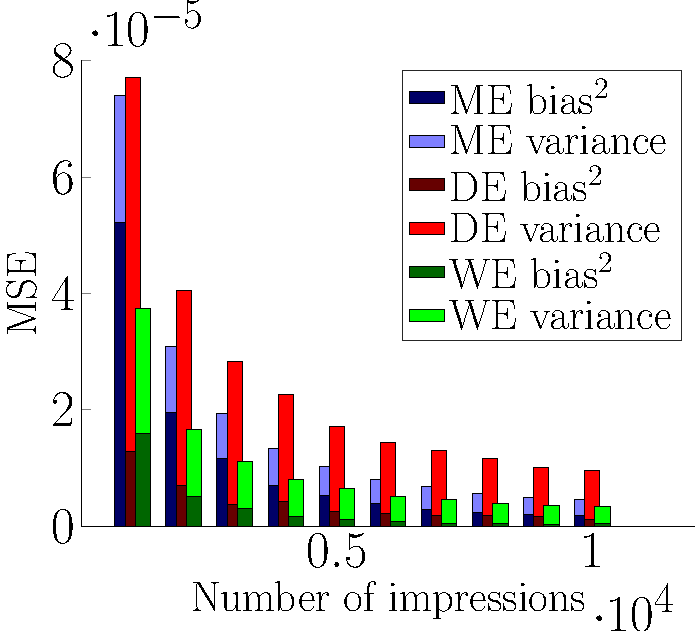
\includegraphics[scale=.425]{./img/internetAds-impressions.pdf}}
    \subfigure[Increasing number of ads.\label{F:ia_second}]{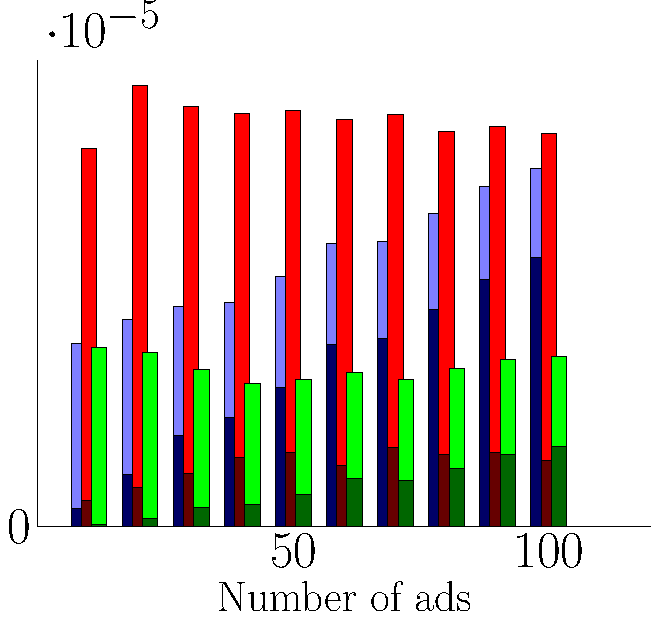
\includegraphics[scale=.425]{./img/internetAds-actions.pdf}}
    \subfigure[Increasing value of maximum CTR.\label{F:ia_third}]{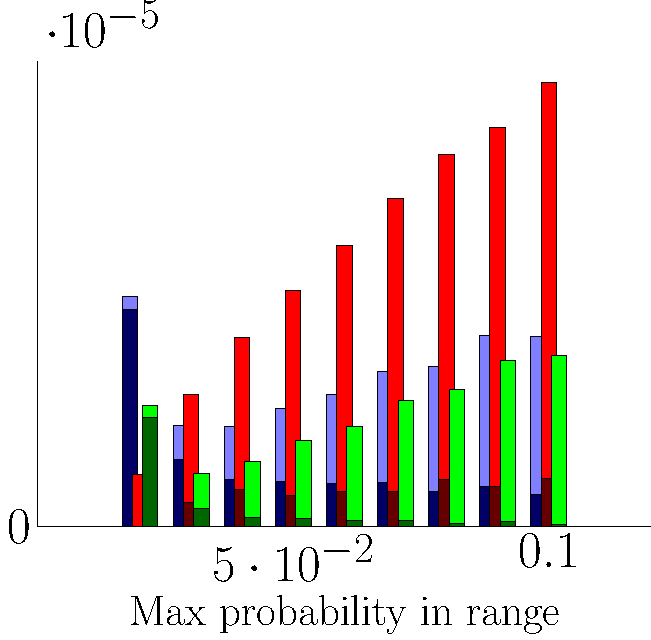
\includegraphics[scale=.425]{./img/internetAds-probs.pdf}}
    \caption[Internet ads results]{MSE for each setting. Results are averaged over 2000 experiments.}\label{F:iAds}
    \end{minipage}
\end{figure*}

In Figure \ref{F:iAds}, we show the $MSE = bias^2 + variance$ for the three settings comparing the results obtained by each estimator. 
In the first setting (Figure~\ref{F:ia_first}) reasonably the \gls{mse} decreases for all estimators as the number of impressions increases and WE has the lowest \gls{mse} in all cases. Interestingly, the \gls{me} estimator has a very large bias in the leftmost case, showing that the \gls{me} estimator suffers large bias when the variances of the sample means are large due to lack of samples (as showed also in Figure \ref{F:absolute_bias}).
Figure~\ref{F:ia_second} shows that an increasing number of actions has a negative effect on \gls{me} and a positive effect on the \gls{de} due to the fact that a larger number of ads implies a larger number of variables with a mean close to the \gls{mev} that represents a worst case for \gls{me} and a best case for \gls{de}. 
The \gls{mse} of \gls{we} is the lowest in all cases and does not seem to suffer the increasing number of actions. 
The same happens in Figure~\ref{F:ia_third} when all the ads share the same click rate (0.02), where \gls{de} is the best.
However, it starts to have large variance as soon as the range of probabilities increases (Figure \ref{F:variance}). 
The \gls{mse} of \gls{we} is the lowest \gls{mse}, but it gets similar to the \gls{mse} of \gls{me} as the range increases.

\subsubsection{Sponsored Search Auctions}
We consider this \gls{mab} problem as described in~\cite{xu2013mab}. In this problem a search engine runs an auction to select the best ad to show from a pool of candidates with the goal of maximizing over a value that depends on the bid of each advertiser and its click probability. 
When an ad is clicked, the advertiser is charged from the search engine of a fee that depends on the bids $b$ of the advertisers and the \glspl{ctr} $\rho$ of the ads. 
\glspl{ctr} are generally unknown, therefore the search engine should use data to estimate which is the best ad (i.e., the one that maximizes $b\cdot\rho$) and the payment in case of click; reasonably, wrong estimations may significantly harm the revenue.
On the other hand, the advertisers have to decide the value of their bid $b_i$ according to the true values $v_i$ of a click. A desirable condition in auctions, called \textit{incentive compatibility}, requires that the advertisers maximize their utility by truthfully bidding $b_i = v_i$. Incentive compatibility may not occur when the estimate of the click probabilities are not accurate. We want to evaluate how the estimators favor the incentive compatibility.
We measure the utility gain of advertiser $1$, whose true per click value is $v_1 = 1$, for different bid $b_1$ values and competing with four other advertisers whose bids are $b_{-1} = \lbrace 0.9, 1, 2, 1 \rbrace$. The \glspl{ctr} are: $\rho = \lbrace 0.15, 0.11, 0.1, 0.05, 0.01 \rbrace$. 
\glspl{ctr} are estimated from data collected using the UCB1 algorithm~\cite{auer2002finite} in a learning phase consisting of $10000$ rounds of exploration (i.e. impressions), as done in~\cite{xu2013mab}.

\begin{figure}[t]
    \begin{minipage}{\columnwidth}
    \centering 
    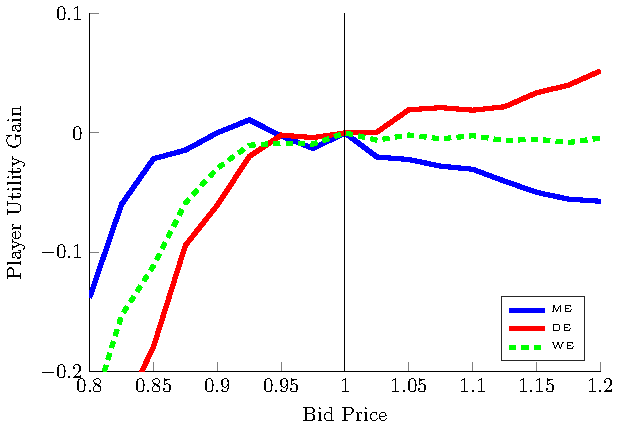
\includegraphics[scale=0.9]{./img/sponsoredSearch.pdf}
    \caption[Sponsored search auctions results]{Relative player 1 utility gain for different value of the bid defined as $\frac{utility(b)}{utility(v)} - 1$. Results are averaged over 2000 experiments.}\label{F:spSearch}
    \end{minipage}
\end{figure}

Figure \ref{F:spSearch} shows the utility gain of advertiser $1$ when using \gls{me}, \gls{de} and \gls{we}.\footnote{The debiasing algorithm proposed in~\cite{xu2013mab} is a cross validation approach, but differs from the estimators considered in this paper. It averages the values used for selection and the values used for estimation, thus being a hybrid of \gls{de} and \gls{me}.}
The true bid price is highlighted with a black vertical bar. \gls{me} results to be only one not able to achieve incentive compatibility, since the utility has positive values before the true bid price. On the contrary with \gls{de} and \gls{we} the advertiser has no incentive to underbid, but there is an incentive to overbid using \gls{de}. Therefore \gls{we} is the only estimator which succeeds to achieve incentive compatibility.

\subsubsection{Grid World}
This simple \gls{mdp} consists of a $3 \times 3$ grid world where the start state in the lower-left cell and the goal state in the upper-right cell~\cite{van2010double}. 
In this domain, we compare the three estimators together with the performance of an algorithm called Bias-corrected $Q$-Learning, a modified version of $Q$-learning that, assuming Gaussian rewards, corrects the positive bias of \gls{me} by subtracting to each $Q$-value a quantity that depends on the standard deviation of the reward and on the number of actions~\cite{lee2012intelligent,lee2013bias}. Moreover, we test Weighted $Q$-Learning also using a different policy, that we call \textit{weighted policy}, which samples the action to perform in a state from the probability distribution of the weights of WE.
We use an $\varepsilon$-greedy policy with $\varepsilon = \frac{1}{\sqrt{n(s)}}$ where $n(s)$ is the number of times the state $s$ has been visited.
Learning rate is $\alpha_t(s, a) = \frac{1}{n_t(s, a)^{0.8}}$ where $n_t(s, a)$ is the current number of updates of that action value and the discount factor is $\gamma = 0.95$. 
In Double $Q$-Learning we use two learning rates $\alpha_t^A(s, a) = \frac{1}{n_t^A(s, a)^{0.8}}$ and $\alpha_t^B(s, a) = \frac{1}{n_t^B(s, a)^{0.8}}$ where $n_t^A(s, a)$ and $n_t^B(s, a)$ are respectively the number of times when table A and table B are updated. 
The reward function is considered in three different settings: Bernoulli, $-12$ or $10$ randomly at each step, Gaussian with mean $\mu = -1$ and standard deviation $\sigma = 5$, Gaussian with mean $\mu = -1$ and standard deviation $\sigma = 1$. 
Once in the goal state, each action ends the episode and returns a reward of $5$. The optimal policy ends the episode in five actions, therefore the optimal average reward per step is $0.2$. Moreover, the optimal value of the action maximizing the $Q$-value is $5\gamma^4 - \sum_{k=0}^3 \gamma^k \approx 0.36$.
In Figure \ref{F:grid}, the top plots show the average reward per step obtained by each algorithm and the plots at the bottom show the estimate of the maximum state-action value at the starting state for each algorithm.
\begin{figure*}
  \begin{minipage}{\textwidth}
    \centering
    \subfigure[Bernoulli.\label{F:bernoulli}]{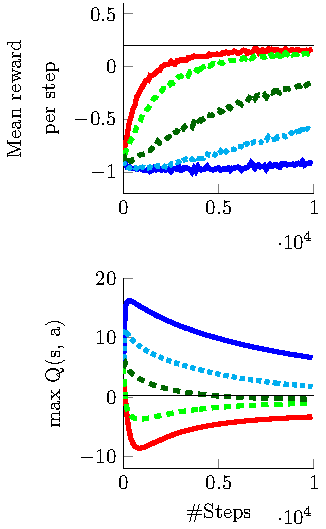
\includegraphics{./img/gridexp08-ng.pdf}}
    \hspace{-.5cm}
    \subfigure[$\mathcal{N}(-1, 5)$.\label{F:gaussian5}]{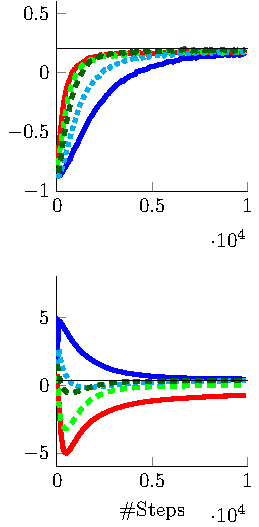
\includegraphics{./img/gridexp08-g.pdf}}
    \hspace{-.5cm}
    \subfigure[$\mathcal{N}(-1, 1)$.\label{F:gaussian1}]{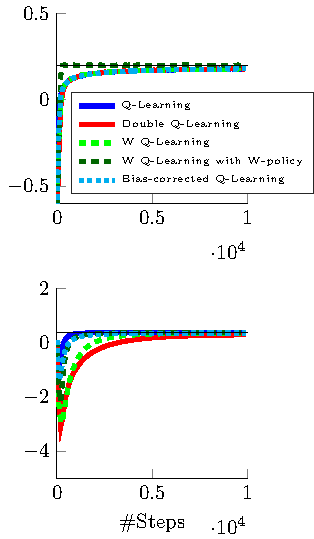
\includegraphics{./img/gridexp08-g-sigma1.pdf}}
    \caption[Grid world results]{Grid world results with the three reward functions averaged over 10000 experiments. Optimal policy is the black line.}\label{F:grid}
  \end{minipage}
\end{figure*}
Figures~\ref{F:bernoulli} and~\ref{F:gaussian5} show that, regardless of the bad approximation of the $Q$-function, the underestimation of Double $Q$-Learning allows to learn the best policy faster than other algorithm in these noisy settings.
Bias-corrected $Q$-Learning estimates the $Q$-function better than Double $Q$-Learning, but performs worse than the other algorithms, except for $Q$-Learning, when the variance is large.
Weighted $Q$-Learning shows much less bias than the other estimators in all settings; moreover, the use of the weighted policy generally reduces the bias of the estimation and achieves the best performance in the case with $\sigma = 1$ (see Figure~\ref{F:gaussian1}). These good results are explained considering that the weighted policy is able to reduce the exploration faster than $\varepsilon$ greedy due to exploiting of the good approximation of the $Q$-function computed by Weighted $Q$-Learning. It is worth to point out that Weighted $Q$-Learning works well for both Gaussian and Bernoullian rewards, showing that WE is effective even with non-Gaussian distributions even if it uses a Gaussian approximation of $Q$-values,

\begin{figure*}
\begin{minipage}{\textwidth}
\centering
\subfigure[Training phase.\label{F:forex_train}]{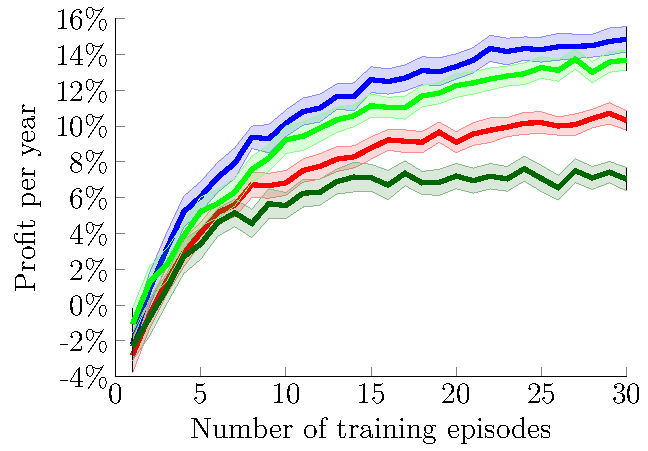
\includegraphics[scale=0.6]{./img/forexTrain.pdf}}
\subfigure[Test phase.\label{F:forex_test}]{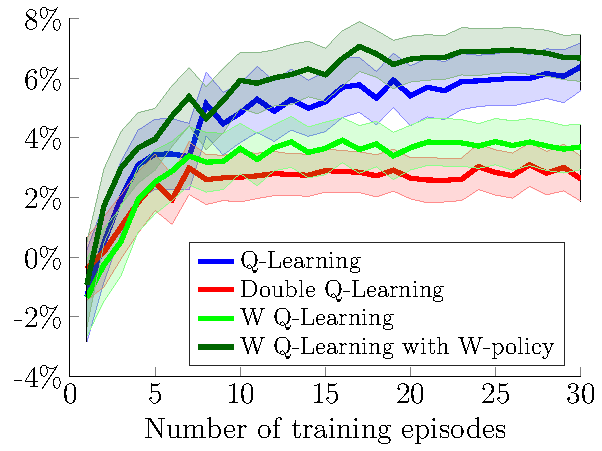
\includegraphics[scale=0.6]{./img/forexTest.pdf}}
\end{minipage}
\caption[Forex results]{Profit per year averaged over 100 experiments.}\label{F:forex}
\end{figure*}

\subsubsection{Forex}
We evaluate the performance of the three estimators in a more challenging discrete \gls{mdp}.
We build an \gls{mdp} based on the Foreign Exchange Market (Forex), an environment with acknowledged hardly predictable dynamics that complicate the estimate of the $Q$-values and, therefore, of the expected profit. The \gls{mdp} we build is a simplified version of the real Forex market. In our Forex \gls{mdp} the agent enters in the market always with 1\$ and each time the agent enters on long or short position a fixed spread value of 0.0002\$ is paid.
The possible actions taken from the agent can be -1, 0 or 1, which mean respectively \textit{'enter on a short position'}, \textit{'close a position'} and \textit{'enter on long position'}.
The state space is composed of the suggestion (in terms of actions) provided by 7 common Forex indicators and the action chosen by the agent at the previous time step.
The state space is $S = \lbrace -1, 0, 1 \rbrace ^8$ with $s_{i = 1...7}(t) = \lbrace -1, 0, 1 \rbrace$ and $s_8(t) = a(t - 1)$.
The action taken by the agent is $a(t) = \lbrace -1, 0, 1 \rbrace$.
The reward $r(t)$ is a function of the previous and current action chosen and of the difference between the current closing price $c(t)$ and the previous closing price $c(t - 1)$:
$$r(t) = a(t - 1)(c(t) - c(t - 1)) + 0.5 * spread |a(t) - a(t - 1)|.$$
The same algorithms used in the grid world, except for Bias-Corrected $Q$-Learning, domain were trained using historical daily data of GBP/USD exchange rate from 09/22/1997 to 01/10/2005 and tested on data from 01/11/2005 to 05/27/08. 
During the training phase, we set learning rate $\alpha(s,a)=\frac{1}{n(s, a)}$, discount factor $\gamma=0.8$ and $\varepsilon=\frac{1}{\sqrt{n(s)}}$.

Figure \ref{F:forex} shows the profit per year, w.r.t. the number of training episodes, of the four algorithms during the training phase (Figure~\ref{F:forex_train}) and during a test phase where the learned policy is run with a greedy policy (Figure~\ref{F:forex_test}). In the training phase an $\varepsilon$-greedy policy is used for $Q$-learning and Double $Q$-Learning, while Weighted $Q$-Learning uses both the $\varepsilon$-greedy policy and the weighted policy.
During the training phase, $Q$-learning performs better than Double $Q$-learning and also than Weighted $Q$-learning. Interestingly, Weighted $Q$-learning with the weighted policy reaches the worst performance in the training phase, but it reaches the best performance in the test phase. This happens because more exploration is induced by the weighted policy w.r.t. the $\varepsilon$-greedy policy, resulting in bad performance during the training phase, but also in better estimates of the $Q$-values.
Double $Q$-learning performs worse than $Q$-learning and Weighted $Q$-learning both in training phase and test phase. 
The reason is that in many states there is an action that is significantly better than the others, that represents the case where \gls{me} gives the best results, and the case where \gls{de} suffers the most.

\subsection{Continuous state spaces}
\begin{figure*}
 \begin{minipage}{.99\columnwidth}
 \centering
  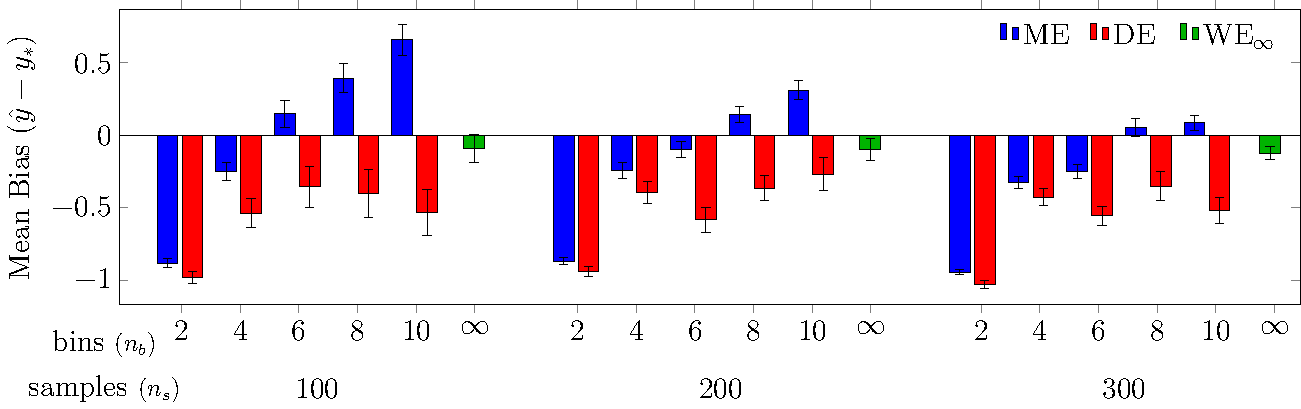
\includegraphics[width=\textwidth]{./img/MM_123_new_noabs.pdf}\\
  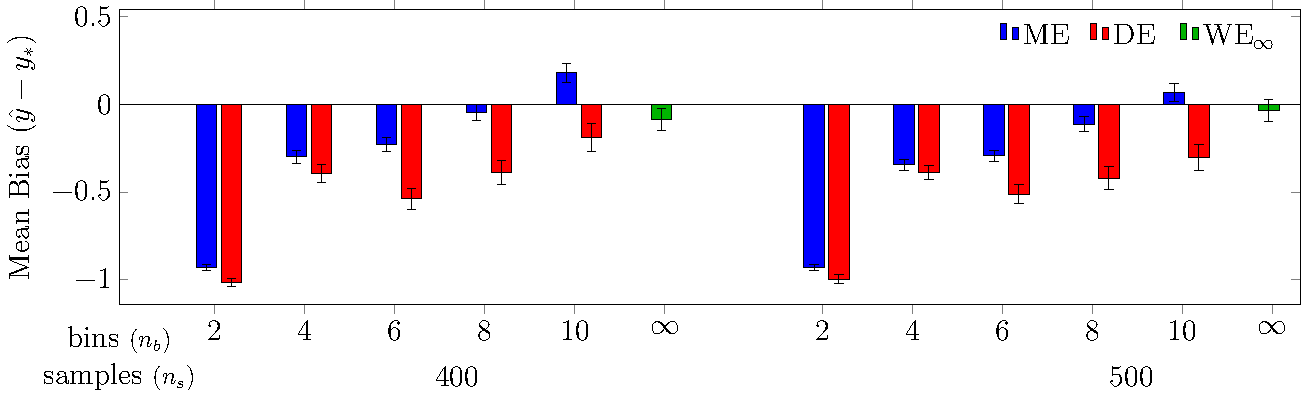
\includegraphics[width=\textwidth]{./img/MM_45_new_noabs.pdf}
 \end{minipage}
  \caption[Bias in pricing problem]{Mean bias obtained by ME, DE and $\text{WE}_{\infty}$ with different sample sizes  and bins (only for ME and DE).
  }
  \label{F:pricing_bias}
\end{figure*}
\begin{figure*}[t]
 \begin{minipage}{.99\columnwidth}
 \centering
  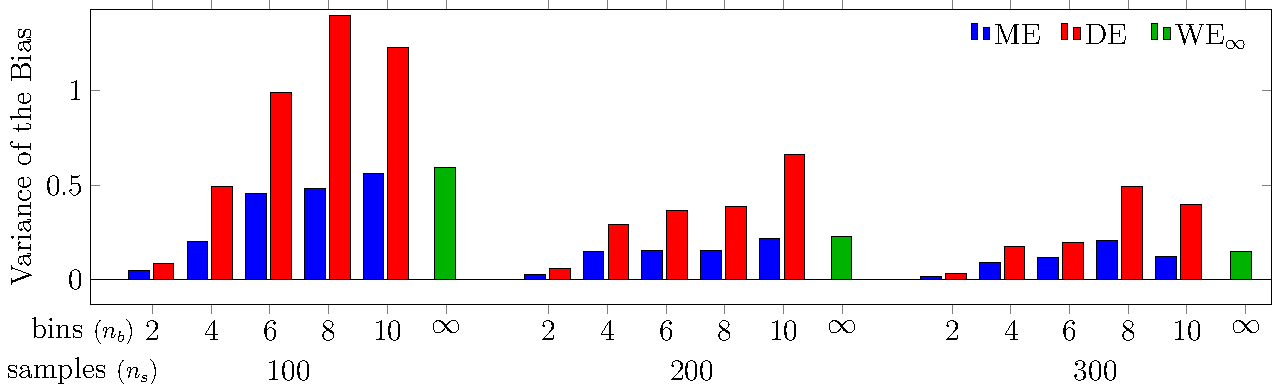
\includegraphics[width=\textwidth]{./img/MM_123_new_var.pdf}\\
  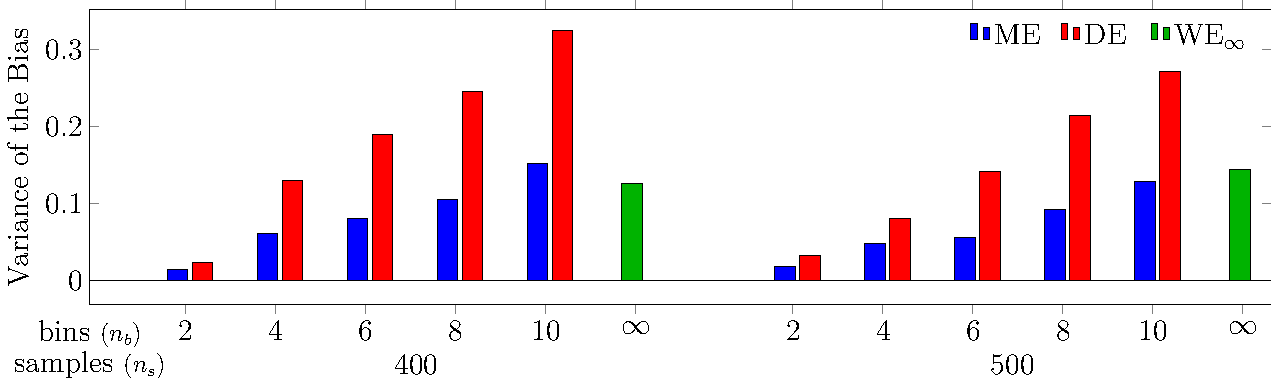
\includegraphics[width=\textwidth]{./img/MM_45_new_var.pdf}
 \end{minipage}
  \caption[Variance in pricing problem]{Variance of the bias obtained by ME, DE and $\text{WE}_{\infty}$ with different sample sizes and bins.
  }
  \label{F:pricing_variance}
\end{figure*}
\subsubsection{Pricing Problem}
This problem consists in estimating the \gls{mev} of the gross profit in a pricing problem. In this \gls{mab} problem we validate the \gls{we} with infinite random variables ($\text{WE}_{\infty}$) and we compare its performance against \gls{me} and \gls{de} whose support (actions) has been discretized.
It is crucial to estimate the value of the gross profit accurately in order to evaluate, for example, an investment decision or to analyze the profitability of products.
The support (action) space is bounded but continuous, and represents the price $p$ to be shown to the user ($p \in [0,10]$).
The reserve price $\tau$ , which is the highest price that a buyer is willing to pay, is modeled as a mixture of $3$ Gaussian distributions with mean $\mu=\lbrace 2, 4, 8 \rbrace$, covariances $\sigma^2= \lbrace 0.01, 0.01, 0.09 \rbrace$ and weights $w = \lbrace 0.6, 0.1, 0.3 \rbrace$.
The revenue function $r_{\tau}(p)$ is $p$ when $\tau \geq p$ and $0$ otherwise.
The maximum revenue is about $2.17$.
In each test the algorithms are fed with a set of samples $\mathcal{D} = \left\{ \langle p_i, r_i \rangle \right\}_{i=1}^{n_s}$. Each sample is obtained by sampling a reserve price $\tau_i$ from the Gaussian mixture, a price $p_i$ from a uniform distribution over the price range, and by evaluating the revenue function ($r_i=r_{\tau_i}(p_i)$). Clearly, the reserve price is unknown to the algorithm.
Results are averaged on $50$ runs in order and confidence intervals at $95\%$ are shown.
\gls{we} exploits a Gaussian process with squared exponential kernel to generalize over the continuous price (\gls{gp} parameters are learned from $\mathcal{D}$), while \gls{me} and \gls{de} discretize the price space into $n_b$ uniformly spaced bins.
As shown in Figure~\ref{F:pricing_bias}, the number $n_b$ of optimal bins varies with the number $n_s$ of available samples.
This means that, once the samples have been collected, \gls{me} and \gls{de} need an optimization phase for selecting the appropriate number of bins (not required by \gls{we}). 
\gls{we} is able to achieve the lowest or a comparable level of bias with every batch dimension even through it exploits a sensibly wider action space (infinite).
In fact, as shown by the experiments, the performance of \gls{me} and \gls{de} may degrade as the number of bins increases, i.e. the action space increases.
This means that, if you want to be accurate, you cannot increase the number of bins arbitrarily (it is somehow counterintuitive).
Additionally, Figure~\ref{F:pricing_variance} shows that the higher complexity of \gls{we} has practically no impact on the variance of the estimate.
The variance is always comparable to the one of the best configuration of \gls{we} and \gls{de}.
Finally, several applications do not consider positive and negative bias to be the same, in particular, in iterative application positive bias can lead to large overestimates that have proven to be critical (e.g. in \gls{rl}).
This is not the case because this pricing problem is not iterated. From Figure~\ref{F:pricing_bias} we can see that \gls{me} is prone to provide positive bias, while \gls{we} bias is almost always the smaller or stays between \gls{me} and \gls{de}.
The reason for which the \gls{me} bias is not always positive, as stated by its theoretical property (for finite case), is due 
to the use of binning for the discretization of the continuous \gls{mab}.
This discrete approximation introduces an additional (here negative) term to the bias.

\subsubsection{Swing-Up Pendulum}
A more complex scenario is represented by the continuous control problem analyzed in this section: the Swing-Up Pendulum with limited torque~\cite{doya2000reinforcement}.
The aim of these experiments is to compare the newly proposed extensions of \gls{fqi} (\gls{dfqi} and \gls{wfqi}) in a continuous state domain with both discrete and continuous actions.
The peculiarity of this domain resides in the fact that the control with a limited torque ($u \in [-5,5]$) makes the policy learning non-trivial.
The continuous state space is $x = (\theta, \omega)$, where $\theta$ is the angle and $\omega$ is the angular velocity.
An episode starts with $x_0 = (\theta_0, 0)$ where $\theta_0 \sim \mathcal{U}(-\pi, \pi)$, evolves according to the the dynamic system $\dot{\theta}=\omega$ and $ml^2\dot{\omega}=-\mu\omega + mgl \sin(\theta) + u$, and terminates after $100$ steps. The physical parameters are mass $m=1$, length $l=1$, $g=9.8$, step time $\tau_0=0.01$.
\begin{figure*}
\begin{minipage}{\textwidth}
\centering
\subfigure[Discrete actions.\label{F:pendulum_discrete}]{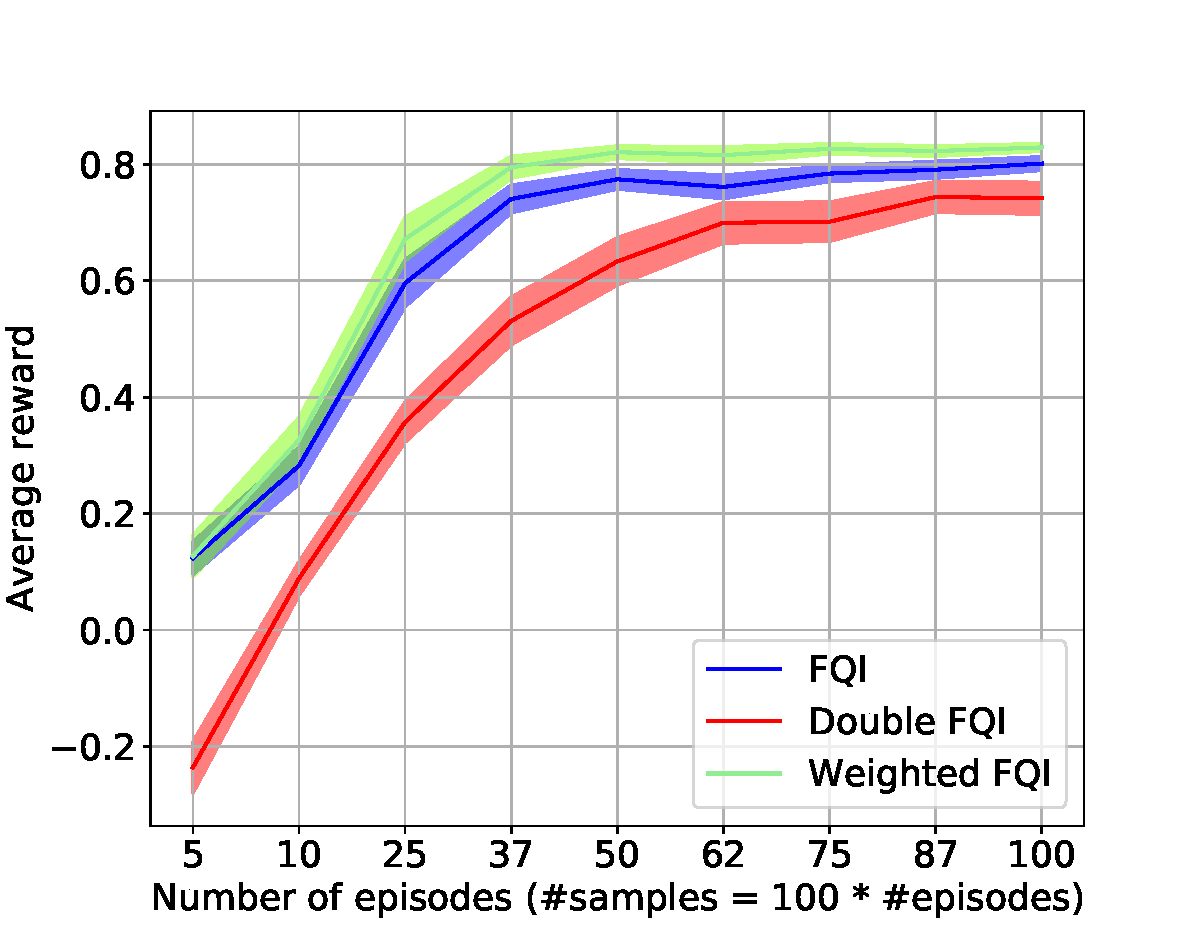
\includegraphics[scale=0.35]{./img/pendulumDiscrete.pdf}}
\hspace{-.5cm}
\subfigure[Continuous actions.\label{F:pendulum_continuous}]{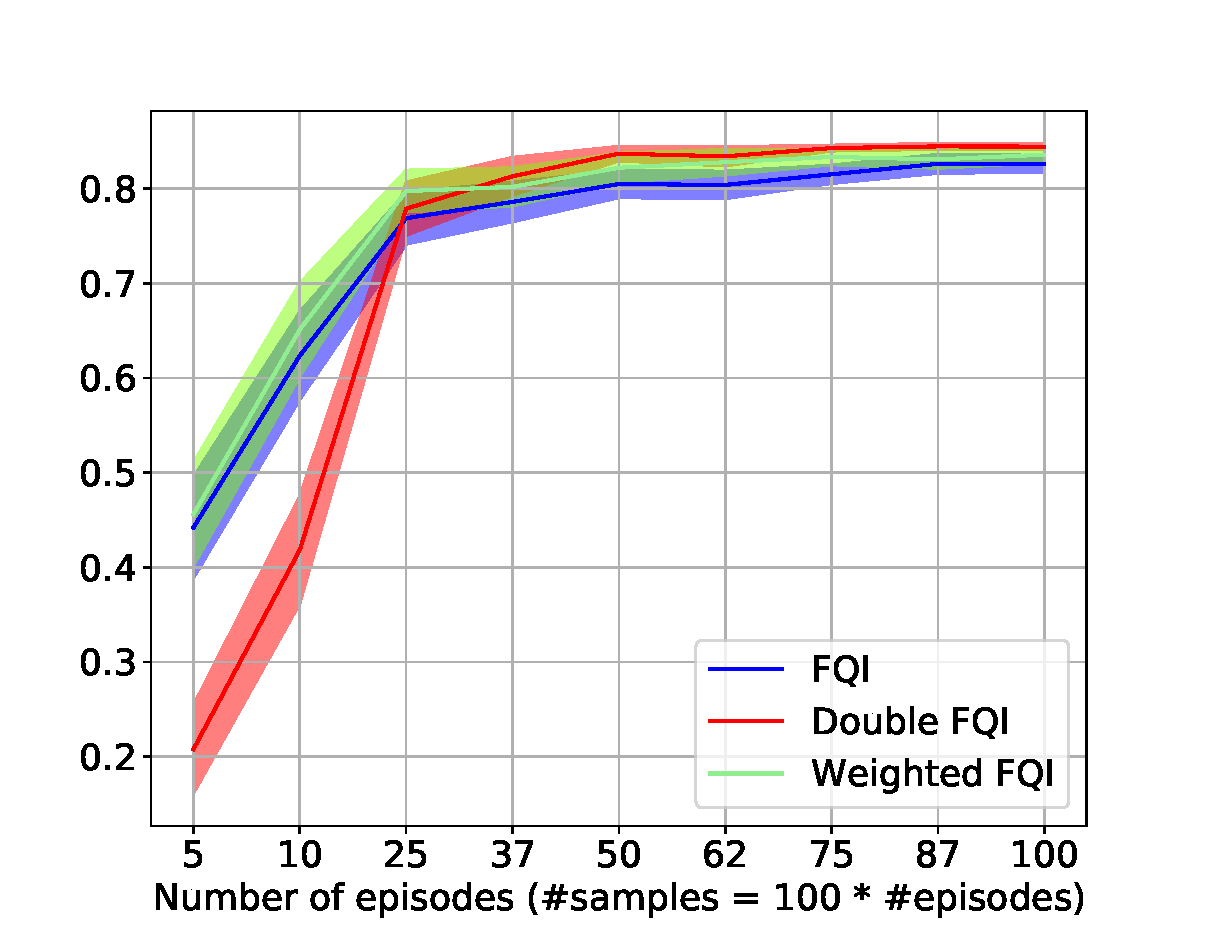
\includegraphics[scale=0.35]{./img/pendulumContinuous.pdf}}
\end{minipage}
\caption[Swing-up pendulum results]{Swing-up pendulum performance averaged over $100$ experiments.}\label{F:pendulum}
\end{figure*}
The reward depends on the height of the pendulum: $r(x) = \cos(\theta)$.
The problem is discounted with $\gamma = 0.9$.
The \gls{gp} uses a squared exponential kernel with independent length scale for each input dimension (ARD SE). The hyperparameters are fitted on the samples and the input values are normalized between $[-1,1]$.
We collected training sets of different sizes using a random policy.
The \gls{fqi} horizon is $10$ iterations.
The final performance of the algorithm is the \emph{average reward}, calculated starting from $36$ different initial angles $\theta_0 = \lbrace \frac{2\pi k}{36} | k=\left\{0, 1, \ldots, 35\right\}\rbrace$.
We consider two settings of this problem: one with a discrete set of 11 uniformly spaced torque values in $[-5,5]$ and another with a continuous action space.
In the former setting we use a different \gls{gp} for each action.
Figure~\ref{F:pendulum} show that \gls{wfqi} for discrete actions \ref{A:WFQI} and \gls{fqi} are robust with respect to the number of episodes and \gls{wfqi} reaches the highest average reward in each case (with statistical confidence obtained over $100$ runs and level $95\%$).
\gls{dfqi} performance is reasonably poor with few examples since it uses a half of the training set to train each regressor.
In the latter setting, the only algorithm that is able to directly handle continuous space is the \gls{wfqi} defined in Algorithm~\ref{A:continuousWFQI}.
The other algorithms use a \gls{gp} with $100$ actions to approximate the maximum.

\subsection{Deep Reinforcement Learning Scenario}
\subsubsection{Acrobot}
\begin{figure}[t]
  \centering
  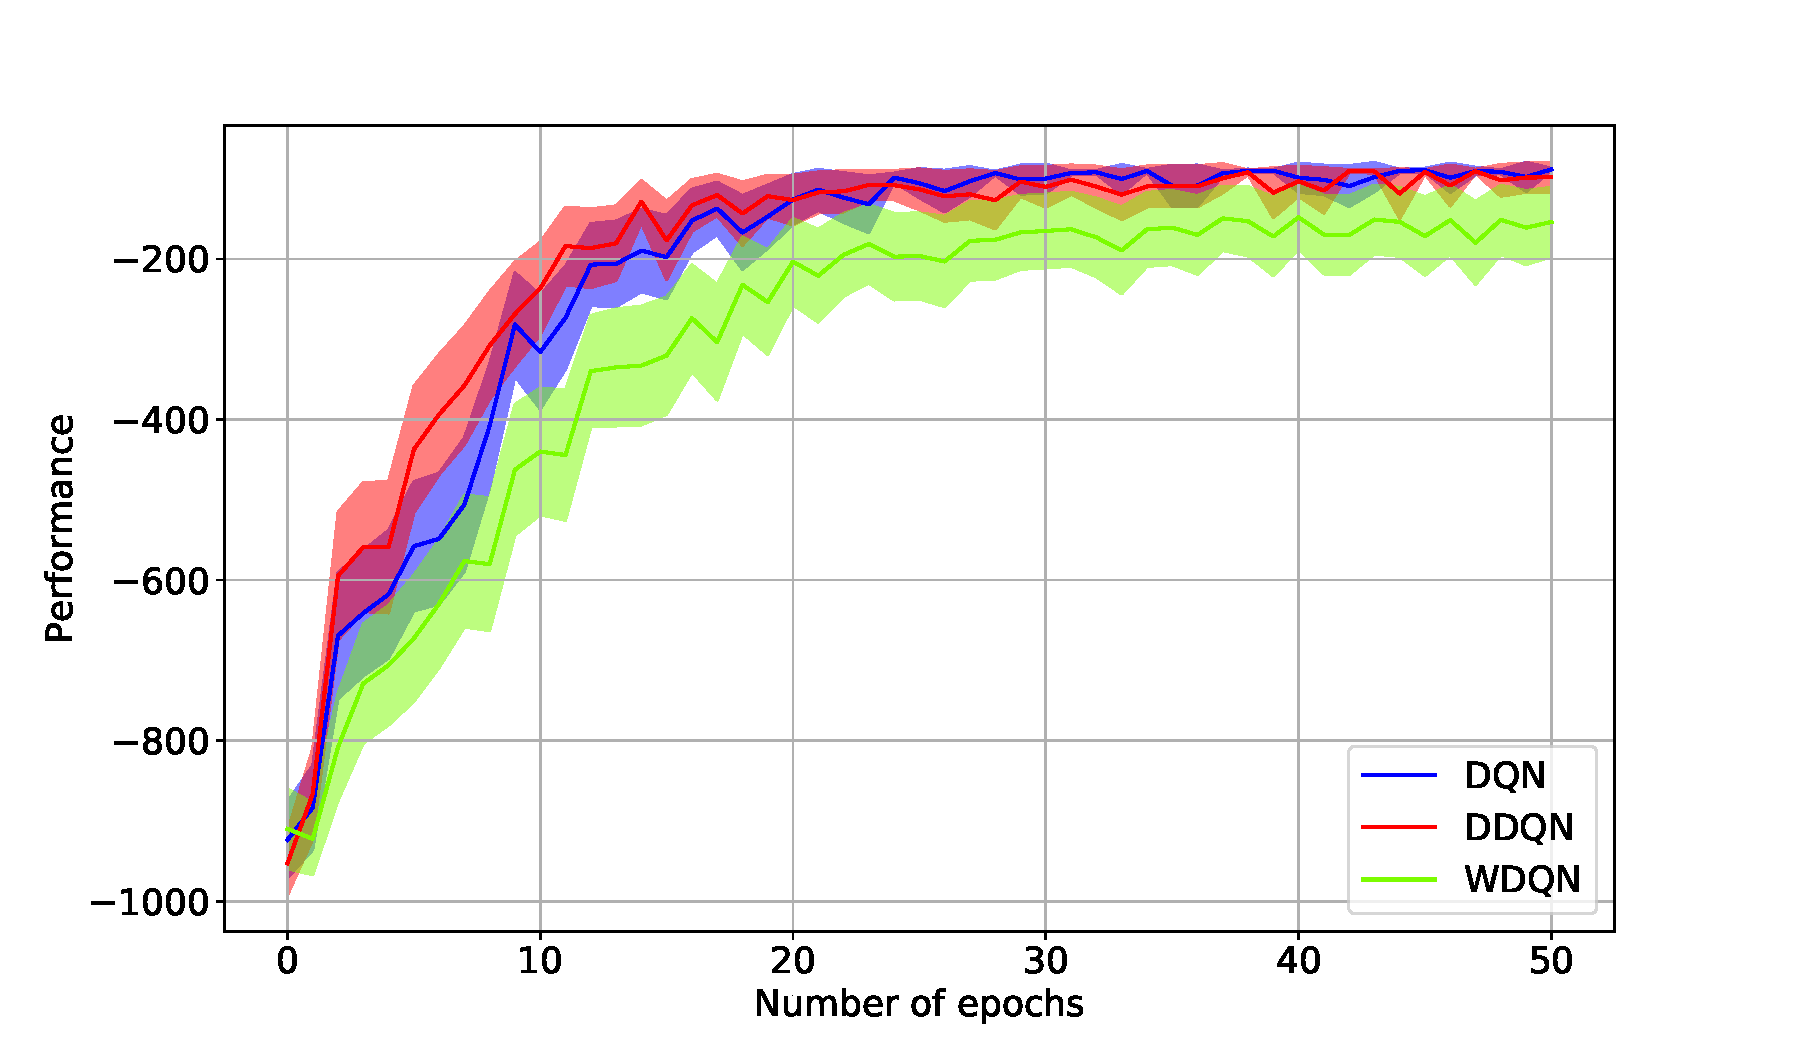
\includegraphics[scale=.35]{./img/acrobot.pdf}
  \caption[Acrobot results]{Acrobot performance averaged on $100$ experiments.
  }
  \label{F:acrobot_wdqn}
\end{figure}
We evaluate the performance of \gls{dqn}, \gls{ddqn} and \gls{wdqn} on the \gls{rl} problem of Acrobot. This is a well-known problem consisting in swinging up a two-link robot over a certain threshold. The state space and the dynamics of the problem make it a complex \gls{mdp} to be solved\footnote{We use the Acrobot-v1 environment of the OpenAI Gym library~\cite{gym}.}. The reward of the \gls{mdp} is $-1$ at each step and $0$ when the arm of the bot reaches the threshold height. The discount factor is $\gamma = 0.99$. The horizon is set to $1000$. The hyperparameters of the training are specified in Table~\ref{T:acrobot_pars}.

\begin{table*}[t]
 \centering
 \caption{Hyperparameters setting in the Acrobot experiment.}
 \label{T:acrobot_pars}
\begin{small}
\setlength{\tabcolsep}{4pt}
 \begin{tabular}{|c|c|}
\hline
Replay memory size & 5000\\
\hline
Initial replay size & 100\\
\hline
Agent history length & 1\\
\hline
Target network update frequency & 100\\
\hline
Masking probability $p$ & $1$\\
\hline
Number of hidden layers & 2\\
\hline
Number of neurons & 80\\
\hline
Number of heads & 10\\
\hline
Test samples & 5000\\
\hline
Evaluation frequency & 1000\\
\hline
Initial exploration rate & 1\\
\hline
Final exploration rate & 0.05\\
\hline
Final exploration frame & 5000\\
\hline
Max no-op actions & 0\\
\hline
Total number of steps & 50000\\
\hline
Optimizer & Adam\\
\hline
 \end{tabular}
 \end{small}
\end{table*}

The results shown in Figure~\ref{F:acrobot_wdqn} are not satisfying in this problem and we still need to investigate the reasons of this. Moreover, we plan to evaluate the performance of \gls{wdqn} in more complex problems such as Atari games.

\chapter{Exploiting uncertainty of the Bellman operator components to deal with highly stochastic problems}
It is well known that a key issue of \gls{rl} applications is the accuracy of the estimation of the action-value with a limited number of samples. Although most algorithms guarantee the convergence of the estimates to the optimal action-value with infinite samples, in practice the presence of stochastic components leads to slow learning. Actually, the majority of real-world problems have significant sources of stochasticity: the environment could have stochastic transitions and this may affect the estimation of the effectiveness of an action; most of the times it is necessary to use stochastic policies to guarantee that all states are potentially visited infinitely many times; the reward function is often corrupted by noisy observations and, in other cases, the reward function is stochastic itself. Moreover, it usually happens that some deterministic environments are partially observable and, thus, are perceived by the agent as stochastic decision processes (e.g. Blackjack).

Since Monte-Carlo estimates of action-values are affected by high variance of the returns, the most successful \gls{rl} algorithms are based on bootstrapping (e.g. Q-Learning~\cite{watkins1989learning}), that trades off the variance of the estimation with a consistent, but biased estimator. However, with a finite number of samples, the bias of the estimation could be significantly relevant when propagating the action-values to the next state and, recursively, to all the other states. Recent works tried to deal with this issue, in particular focusing on the estimation of the maximum expected value. 
It is well known~\cite{smith2006optimizer, van2004rational} that the maximum operator (used in the Q-Learning update equation) is positively biased, thus it overestimates the optimal action-value. In highly stochastic environments, this overestimation leads to unstable learning and poor convergence rates. In order to avoid this issue, the Double Q-Learning algorithm~\cite{van2010double} has been proposed. This algorithm uses the double estimator~\cite{van2013estimating} to compute the maximum action-value to calculate the temporal-difference error: providing a negatively biased estimation (i.e. underestimating) of the maximum action-value, this approach can improve the performance especially in noisy environments. In recent works, a Deep Learning extension of Double Q-Learning~\cite{van2016deep} outperformed the \gls{dqn} algorithm~\cite{mnih2015human}, showing the advantages of the double estimator also in more complex architectures.
A recently proposed approach is the Weighted Q-Learning~\cite{deramo2016estimating}, which computes a weighted average of the action-value function estimates balancing underestimation and overestimation. Another related work is the Bias-corrected Q-Learning algorithm~\cite{lee2013bias} that slightly modifies the temporal-difference error to reduce the effect on the bias of the maximum operator.

However, an inaccurate estimation of the action value function does not always imply bad performance; indeed most of the policies are not dependent on the accuracy of the action-values, but instead they rely on their ordering. For instance, in the empirical section of this paper, we show how Speedy Q-Learning algorithm~\cite{NIPS2011_4251} reaches very good performance despite sometimes estimating the action-values very poorly. Starting from these considerations, we address this problem from another point of view. Indeed, we do not focus on the estimation of the maximum expected value, but we care about weighting the new samples according to the uncertainty of the current estimates. 
We consider that it is not sufficient to accurately estimate the maximum expected value of the Q-function of the next state, but we also need to analyze how this information is propagated to other states. The problem of dealing with uncertainty and the propagation of information across the states of the \gls{mdp} has been addressed in many works on \gls{rl}~\cite{mohagheghi2007proportional, Tewari2007}. Some of them consist in tuning the meta-parameters of the learning process according to uncertainty, e.g. the dynamical changes of the environment~\cite{schweighofer2003meta, Kobayashi2009, yoshida2013reinforcement}.
The work proposed in this paper follows this line of research.

The interesting aspect of this approach is that it is possible to use any maximum expected value estimator and that it can be easily extended to an on-policy scenario. Since we believe that the choice of the estimator is not a relevant issue in our approach, we choose the maximum operator as it is the most common.

\section{Preliminaries}
Recalling the optimal action-value function
\begin{align}
 Q^*(x,u)=\underset{\strut\mathclap{x'\sim \mathcal{P}(x'|x,u)}}{\mathbb{E}}\left[ r(x,u,x')+\gamma\max_{u'} Q^*(x',u')\right],
 \label{eq:qopt}
\end{align}
as the expected value is a linear operator, we can always write (\ref{eq:qopt}) as:
\begin{align}
 Q^*(x,u)=\underset{\strut\mathclap{x'\sim \Pmodel(x'|x,u)}}{\mathbb{E}}\left[ r(x,u,x')\right]+\underset{\strut\mathclap{x'\sim \Pmodel(x'|x,u)}}{\gamma\mathbb{E}}\left[ \max_{u'} Q^*(x',u')\right].
 \label{eq:qdec}
\end{align}

Now, let us define two functions, $\Rtilde$ and $\Qtilde$, as:
\begin{align}
 \Rtilde(x,u)&=\underset{\strut\mathclap{x'\sim \Pmodel(x'|x,u)}}{\mathbb{E}}\left[ r(x,u,x')\right], \nonumber\ \\
 \Qtilde(x,u)&=\underset{\strut\mathclap{x'\sim \Pmodel(x'|x,u)}}{\mathbb{E}}\left[\max_{u'} Q^*(x',u')\right].
 \label{eq:rqtilde}
\end{align}
We can give an interpretation of these two functions: $\Rtilde(x,u)$ is the expected immediate reward of the action $u$ in the state $x$; $\Qtilde(x,u)$ is the expected discounted return of the states reached after performing action $u$ in state $x$ (i.e. the expected gain of the reached state).
We can now write the optimal value function as:
\begin{align}
 Q^*(x,u)=\Rtilde(x,u)+\gamma\Qtilde(x,u).
 \label{eq:qdecrqtilde}
\end{align}

Our approach shifts the focus of the \gls{rl} task from finding a good estimator for the optimal action-value function, to the task of finding good estimators for $\Rtilde$ and $\Qtilde$. The main motivation is that the sources of uncertainty of the two components of the action-value function are different: $\Rtilde$ only depends on transition and reward models, while $\Qtilde$ also depends on the optimal policy.
\section{The Proposed Method}
In the following section, we derive our method from (\ref{eq:qdecrqtilde}). We propose the general schema, using the maximum estimator, and we show the relations with the standard Q-Learning update. We call this method RQ-Learning as it decomposes the \gls{td}-Error in a reward component and an action-value component.

% \subsection{Decomposition of the TD error}
% The standard Q-Learning algorithm, given the tuple $(x,u,r,x')$, computes the temporal difference error w.r.t. the current action-value estimates, and then updates such estimate proportionally to the error. The amount of correction in the direction of the new sample is measured by the learning rate: if the learning rate is $1$, the new sample substitutes the old estimate; if the learning rate is $0$, the new sample is discarded and the old estimate is kept unchanged. 
% As shown in (\ref{eq:qdecrqtilde}) the action-value function could be decomposed in two different components. Our method is based on the idea of giving separate estimates for these two components by computing the error w.r.t. each component of the action-value function, instead of computing the \gls{td} error:
% \begin{align}
% \Rtilde_{t+1}(x,u) & \leftarrow\Rtilde_t(x,u)+\alpha_t(R(x,u,x')-\Rtilde_t(x,u)), \label{eq:rtilupdedate}\\
% \Qtilde_{t+1}(x,u) & \leftarrow\Qtilde_t(x,u)+\beta_t(\max_{u'}Q_t(x',u')-\Qtilde_t(x,u)).
% \label{eq:qtildeupdate}
% \end{align}
% Separating the two components of the value function can be useful, as the two components have inherently different sources of stochasticity. Moreover, the information stored in $\Rtilde$ is local to each state-action pair and does not contain the uncertainty of the estimation of other states. Instead, the information stored in $\Qtilde$ depends only on the action-value function of the states that could be reached after performing the action $u$ in the state $x$, which depends, recursively, on the other action-value functions. It is clear that the propagation of uncertain values only affects the $\Qtilde$ component.
% As the actual action value function is the sum of the two estimates, we can write an equivalent update for the Q-value:
% \begin{align}
% Q_{t+1}(x,u)\leftarrow&\Rtilde_t(x,u)+\alpha_t(R(x,u,x')-\Rtilde_t(x,u)) \nonumber\\
%   & +\gamma\left(\Qtilde_t(x,u)+\beta_t(\max_{u'}Q_t(x',u')-\Qtilde_t(x,u))\right) \nonumber\\
% = & Q_t(x,u)+\alpha_t(R(x,u,x')-\Rtilde_t(x,u)) \nonumber\\
%   & +\gamma\beta_t(\max_{u'}Q_t(x',u')-\Qtilde_t(x,u)).
%  \label{eq:cumulativeupdate}
% \end{align}
% 
% \subsection{Analysis of the decomposed update}
% Now, we discuss the relationship of our method with standard temporal difference methods. Let $t$ be the learning step. As a first step of our analysis we can consider the simplest case $\alpha_t=\beta_t$, $\forall t$ by combining (\ref{eq:cumulativeupdate}) and (\ref{eq:qdecrqtilde}) we obtain:
% \begin{align}
% Q_{t+1}(x,u) \leftarrow & Q_t(x,u)+\alpha_t(R(x,u,x')+\gamma\max_{u'}Q_t(x',u')\nonumber\\
%  & - Q_t(x,u)).
% \end{align}
% That is the classical Q-Learning update. 
% 
% We consider now the setting $\alpha_t\geq\beta_t>0$, $\forall t$. Let $\beta_t=\delta_t\alpha_t$, we obtain:
% \begin{align}
% Q_{t+1}(x,u) \leftarrow & Q_t(x,u)+\alpha_t(R(x,u,x')+\gamma\delta_t \max_{u'}Q_t(x',u') \nonumber\\
%   & -(\Rtilde_t(x,u)+\gamma\delta_t\Qtilde_t(x,u))) \nonumber\\
% = & Q_t(x,u)+\alpha_t(R(x,u,x')+\gamma_t'\max_{u'}Q_t(x',u') \nonumber\\
%   & -(\Rtilde_t(x,u)+\gamma_t'\Qtilde_t(x,u))) \nonumber\\
% = & Q_t(x,u)+\alpha_t((R(x,u,x')+\gamma_t'\max_{u'}Q_t(x',u')) \nonumber\\
%   & - Q_t'(x,u))
% \end{align}
% with $\gamma_t'=\gamma\delta_t$. Notice that $Q_t'(x,u)$ is the Q-value at time step $t$, but computed with a different discount factor. If $\beta_t=\delta_t\alpha_t$, then we can see our method as a variable discount factor learning. If we consider that $\delta_t$ increases monotonically in the interval $[0,1]$, our method works by increasing the effective horizon each step starting from trying to solve a greedy myopic problem and moving towards the real one.
% Similar approaches have been used in practice to solve infinite horizon problems when the discount factor is close to $1$ ~\cite{crites1996improving, bao2008infinite, franccois2015discount}.
% 
% Finally, we can observe that, if the reward function and the transition model are deterministic, we can set $\alpha=1$ and consider only $\beta_t=\delta_t$.
% 
% \subsection{Variance dependent learning rate}
% To improve the quality of the estimation, we would like to weight the error of each sample w.r.t. the current estimate depending on how much we trust the current value of our estimate. Thus, we propose a learning rate that depends on the variance of the current variable estimate.
% 
% First of all we need to compute the variance of each estimator. To perform such computation we have to make the assumption that the learning rate is independent from data. This assumption is needed in order to have a closed form for the variance of the estimator, and it works well in practice. We will assume also that the samples $X_i$ are i.i.d., with mean $\mu$ and variance $\sigma^2$. Consider the general form of the estimator:
% \begin{align}
%  \widetilde{X}_{n+1} = (1-\alpha_t)\widetilde{X}_{n}+\alpha_tX_{n}.
% \end{align}
% We now compute the expected value and the variance of this estimator:
% \begin{align}
%  \mathbb{E}\left[\widetilde{X}_{n+1}\right]& = \mu\sum_i^n \alpha_i \prod_{j=i+1}^{n} \left(1-\alpha_j\right)\\
%  \mathrm{Var}\left[\widetilde{X}_{n+1}\right]& = \sigma^2\sum_i^n \alpha_i^2 \prod_{j=i+1}^{n} \left(1-\alpha_j\right)^2 = \sigma^2\omega
% \end{align}
% with $\omega=\sum_i^n \alpha_i^2 \prod_{j=i+1}^{n} \left(1-\alpha_j\right)^2$. Notice also that we can use the sample covariance $S_{n-1}$ of the random variable $X$ to estimate the real covariance $\sigma^2$. It is possible to compute in an incremental way both the sample covariance, in the traditional way, and $\omega$:
% \begin{align}
%  \omega_{n+1}=(1-\alpha_n)^2\omega_n+\alpha_n^2.
% \end{align}
% A weak assumption of this model is that the variables are identically distributed. While this could be true for the reward function, if the \gls{mdp} is stationary, this is not true for the Q-function values whose distribution is affected by the policy and by the current estimates of the other states. However, a good approximation could be to consider data collected in a temporal window in which the distribution is approximately stationary. Using this approach, we can compute the variance of the process in a given time window forgetting old values that can lead to a biased estimation of the current window variance. While this approach is not formally correct, as the derivation of the variance estimates makes the assumption of i.i.d. variables, this approximation leads to very good results in practice as we show in the empirical Section \ref{S:empirical}.
% 
% Finally, we can choose a learning rate that depends on the covariance. Let $\sigma_e^2(t)$ be an estimate of $\mathrm{Var}\left[\widetilde{X}_{t}\right]$. We propose the following learning rate for each component of the action-value function:
% \begin{align}\label{eq:alpha_eq}
%  \alpha_t=\dfrac{\sigma_e^2(t)}{\sigma_e^2(t)+\eta}
% \end{align}
% where $\eta$ is the amount of the estimator variance for which the learning rate is $0.5$ (i.e. when $\sigma_e=\eta$ the learning rate is 0.5). It can be seen as a soft threshold to tune the speed of the decrease of the learning rate w.r.t. the estimator variance.
% 
% If we consider the case $\beta_t=\alpha_t\delta_t$, then we have to use a different learning rate. As we want an increase of the discount factor faster than the decrease of the general learning rate, we can use an exponentially increasing learning rate for the delta parameter:
% \begin{align}\label{eq:delta_eq}
%  \delta_t = e^{\frac{\sigma_e^2}{\eta}\log\frac{1}{2}}
% \end{align}
% where $\eta$ has the same interpretation as in~(\ref{eq:alpha_eq}) thanks to the $\log\frac{1}{2}$ factor.
% 
% \subsection{Discussion on convergence}
% Convergence of the Q-Learning algorithm is guaranteed under some conditions, including some properties on the learning rates ~\cite{EvenDar2001, watkins1992q}:
% \begin{align}
%  0 \leq \alpha < 1,\nonumber \\
%  \lim_{N\rightarrow\infty} \sum_{t=1}^{N}\alpha_t & = \infty,\nonumber \\
%  \lim_{N\rightarrow\infty} \sum_{t=1}^{N}\alpha_t^2 & < \infty. \label{eq:lr_cond}
% \end{align}
% In order to give some preliminary results about the convergence of RQ-Learning and to motivate the choice of the formulas of learning rates $\alpha$ and $\delta$, we show that, under some assumptions, the proposed formulas (\ref{eq:alpha_eq}) (\ref{eq:delta_eq}) satisfy (\ref{eq:lr_cond}). Suppose that the variance of the estimator $\sigma_e^2(t)$ is the variance of the sample mean. It is well known, by the central limit theorem, that the variance of the sample mean is $\sigma_{\mu}(t)=\frac{\sigma^2}{t}$, where $\sigma$ is the variance of the process that generates the samples.
% This assumption does not hold in general, as we can see from the formula of the learning rate; however, this is true for the sample mean, that is a special case of the generic estimator.
% 
% Now, just consider the learning rate proposed in (\ref{eq:alpha_eq}), replacing the variance of the sample mean into the variance of the estimator:
% \begin{align}\label{eq:alpha_smv}
%  \alpha_t=\frac{\sigma^2}{\sigma^2+\eta t}
% \end{align}
% it can be easily shown that:
% \begin{align}
%  \lim_{N\rightarrow\infty} \sum_{t=1}^{N}\frac{\sigma^2}{\sigma^2+\eta t} & = \infty, \\
%  \lim_{N\rightarrow\infty} \sum_{t=1}^{N}\left(\frac{\sigma^2}{\sigma^2+\eta t}\right)^2 & < \infty.
% \end{align}
% Now, consider $\beta_t=\alpha_t\delta_t$. In this scenario, we propose an exponential learning rate. Let be $\alpha_t=\frac{1}{t}$ for simplicity, and consider the learning rate (\ref{eq:delta_eq}) to replace the sample mean into the variance of the estimator:
% \begin{align}\label{eq:beta_delta_smv}
%  \beta(t) = \frac{1}{t}e^{\frac{\sigma^2}{\eta t}\log\frac{1}{2}}.
% \end{align}
% Then:
% \begin{align}
%  \lim_{N\rightarrow\infty} \sum_{t=1}^{N}\frac{1}{t}e^{\frac{\sigma^2}{\eta t}\log\frac{1}{2}} & = \infty, \\
%  \lim_{N\rightarrow\infty} \sum_{t=1}^{N}\left(\frac{1}{t}e^{\frac{\sigma^2}{\eta t}\log\frac{1}{2}}\right)^2 & < \infty.
% \end{align}
% This analysis considers only the estimation of the variance of the sample mean. The analysis of the generic variance estimator is more complex, but we conjecture that convergence could be guaranteed under some mild conditions on $\eta$ and $\sigma$.
% 
% \section{Experimental Results}\label{S:empirical}
% In this section, we highlight the main advantages of exploiting the structure of the \gls{td}-Error with RQ-Learning in three discrete \glspl{mdp}. We compare RQ-Learning against Q-Learning \cite{watkins1992q}, Double Q-Learning \cite{van2010double}, Weighted Q-Learning \cite{d2016estimating} and Speedy Q-Learning\footnote{In these experiments we consider the asynchronous version of Speedy Q-Learning.} \cite{NIPS2011_4251}. We choose this set of algorithms because we want to analyze the impact of the maximum expected value estimator in the learning process. Indeed, while \cite{van2010double} strongly suggests that a negatively biased estimator should be used to deal with stochastic \glspl{mdp}, the  empirical results, reported in the following, show that positively biased estimators are able to achieve better performance in highly stochastic problems as well. Instead, we show that the main point consists in exploiting data in the best way, in particular in the estimation of the action-value, giving higher relevancy to more recent samples. We conjecture that the trade-off between keeping the old estimate and updating it with the new one is the key issue in highly stochastic environments. Both RQ-Learning and Speedy Q-Learning exploit this idea; in particular, the latter uses an increasing learning rate on the difference between the target computed with the current estimation and the one computed with the previous estimation, while RQ-Learning weights the update considering the uncertainty of the current estimation.
% 
% We analyze the performance of RQ-Learning with different choices of learning rates. All the other algorithms use a decaying learning rate $\alpha(s, a) = \frac{1}{n(s, a)^{k}}$ where $n(s, a)$ and $k$ are respectively the number of updates for each action $a$ in state $s$ and a coefficient to tune the rate of decay.\footnote{Assuming that Double Q-Learning splits the action-value table in a table A and a table B, also the learning rate is split in $\alpha_A(s, a) = \frac{1}{n_A(s, a)^{k}}$ and $\alpha_B(s, a) = \frac{1}{n_B(s, a)^{k}}$, where $n_A(s, a)$ and $n_B(s, a)$ are the number of updates for each action $a$ in state $s$, respectively in table A and table B.}
% 
% \subsection{Noisy Grid World}
% This environment, proposed in \cite{van2010double}  and \cite{d2016estimating}, consists of a $3 \times 3$ grid with the initial position in the lower-left cell and the goal state in the upper-right cell. Each action performed in a non-goal state obtains a reward $-12$ and $10$ with equal probability. In the goal state, every action obtains a reward of $5$ and terminates the episode. The discount factor is $\gamma = 0.95$. The policy is $\varepsilon$-greedy with $\varepsilon = \frac{1}{\sqrt{n(s)}}$, where $n(s)$ is the number of  visits of the state $s$. The optimal average reward per step is $0.2$ and the maximum action-value function of the initial state is $5\gamma^4 - \sum_{k=0}^3 \gamma^k \approx 0.36$.
% 
% Figure \ref{F:hasselt_all} shows the mean reward per step and the approximation of the maximum action-value in the initial state computed by the other algorithms and RQ-Learning with $\alpha$ as used by the other algorithms, but with the separated variance-dependent learning rate $\beta$ for the action-value estimate using $\eta = 1$. Notice how the performance of RQ-Learning for the reward is the best one (except for $k=0.8$ where all algorithms perform similarly) and, also, how the estimate of the action-value is the best one. With $k=1$, Speedy Q-Learning outperforms both Double Q-Learning and Weighted Q-Learning considering the mean reward per step, even with a diverging estimate of the action-value function. This is an empirical evidence of our conjecture: the bias of the estimation is not necessarily correlated to the performance. Moreover, as expected, the performance of RQ-Learning is not affected by the exponent used in the learning rate. The other algorithms achieve the optimal performance only in the setting with the higher learning rate, confirming the advantage of giving more importance to newer samples.
% 
% In Figure \ref{F:hasselt_QDecs}, we compare different variants of RQ-Learning: ``RQBeta'' is the same configuration used in Figure \ref{F:hasselt_all}; ``RQDelta'' uses $\beta = \alpha \delta$ with $\eta = 1$; ``RQWin'' uses a windowed estimation of variance with a window of length $50$ and $\eta = 0.5$. ``RQAlphaBeta'' uses a variance-dependent learning rate also for $\alpha$ with $\eta = 100$ and $\beta$ with $\eta = 1$; ``RQWinAlpha'' is the same configuration of the previous one, but uses a windowed $\beta$ with $\eta = 0.5$. Note that $\eta$ has a larger value in configurations without windowed variance estimation because such configurations are likely to overestimate the current variance of the process. ``RQDelta'' configurations result in a cautious learning that leads to very slow improvements, but avoids the overestimation of the action-value slowly converging to the optimal value. While ``RQDelta'' performance is not comparable with other configurations of RQ-Learning, it still outperforms Q-Learning. The other configurations perform similarly to the best one.
% 
% In Figure \ref{F:hasselt_QDecTol} we show the same information of Figure \ref{F:hasselt_all} and \ref{F:hasselt_QDecs} for RQ-Learning with different values of $\eta$ to give a sense of how this parameter influences the learning process. It is clear how lower values of $\eta$ (i.e. a higher learning rate) let the results converge faster, confirming that a high value of the learning rate helps to speedup the learning process in highly stochastic environments like this.
% 
% \begin{figure}[t]
% \begin{minipage}{\columnwidth}
% \centering
%   \subfigure[$\alpha = \dfrac{1}{n(s,a)}$\label{F:hasselt_all_1}]{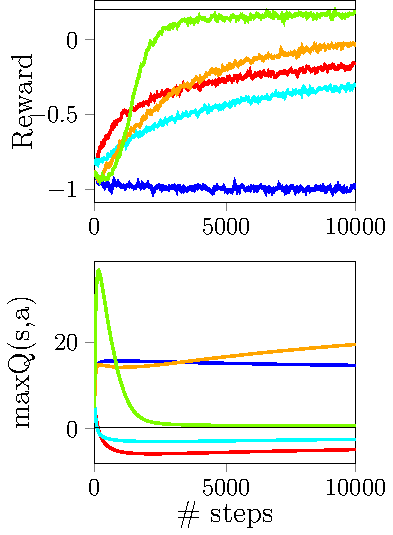
\includegraphics[scale=.7]{./imgs/gridHasselt/allAlgs1.pdf}}\hspace{-.5cm}
%   \subfigure[$\alpha = \dfrac{1}{n(s,a)^{0.8}}$\label{F:hasselt_all_08}]{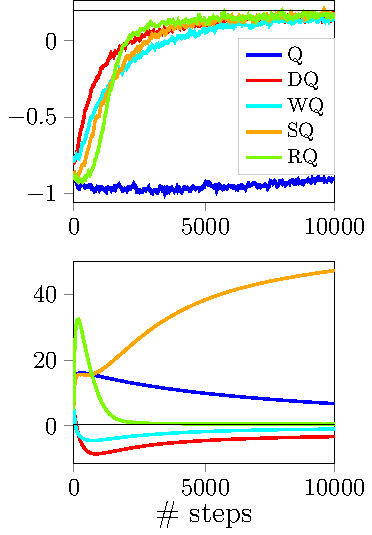
\includegraphics[scale=.7]{./imgs/gridHasselt/allAlgs08.pdf}}
% \end{minipage}
%   \caption{Mean reward per step (top) and maximum action-value estimate in the initial state (bottom) in the Noisy Grid World problem of all the other algorithms and of the best setting of RQ-Learning for this experiment. Results are averaged over $10000$ experiments.}
%   \label{F:hasselt_all}
% \end{figure}
% \begin{figure}[t]
% \begin{minipage}{\columnwidth}
% \centering
%   \subfigure[$\alpha = \dfrac{1}{n(s,a)}$\label{F:hasselt_qdec_1}]{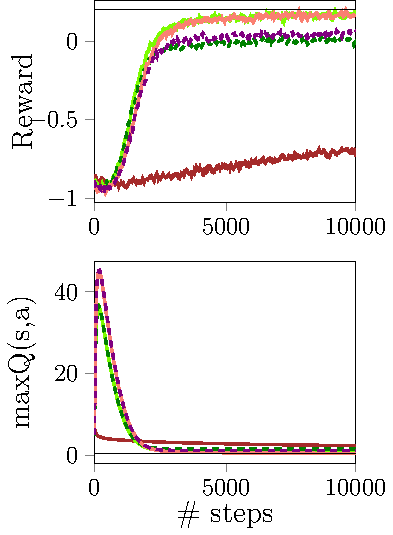
\includegraphics[scale=.7]{./imgs/gridHasselt/QDecs1.pdf}}\hspace{-.5cm}
%   \subfigure[$\alpha = \dfrac{1}{n(s,a)^{0.8}}$\label{F:hasselt_qdec_08}]{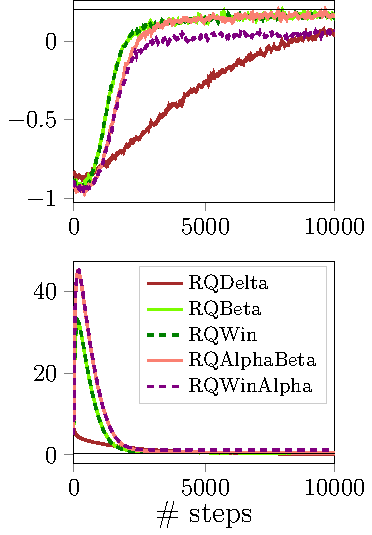
\includegraphics[scale=.7]{./imgs/gridHasselt/QDecs08.pdf}}
% \end{minipage}
%   \caption{Mean reward per step (top) and maximum action-value estimate in the initial state (bottom) in the Noisy Grid World problem of the best setting of RQ-Learning for this experiment together with other less effective setting of RQ-Learning. Results are averaged over $10000$ experiments.}
%   \label{F:hasselt_QDecs}
% \end{figure}
% \begin{figure}[t]
% \begin{minipage}{\columnwidth}
% \centering
%   \subfigure[RQ-Learning{F:hasselt_qdectol}]{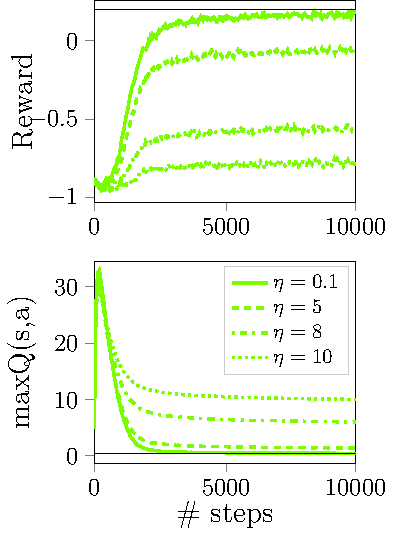
\includegraphics[scale=.7]{./imgs/gridHasseltTol/QDecHasselt.pdf}\hspace{-.5cm}}
%   \subfigure[Windowed RQ-Learning{F:hasselt_qdecwintol}]{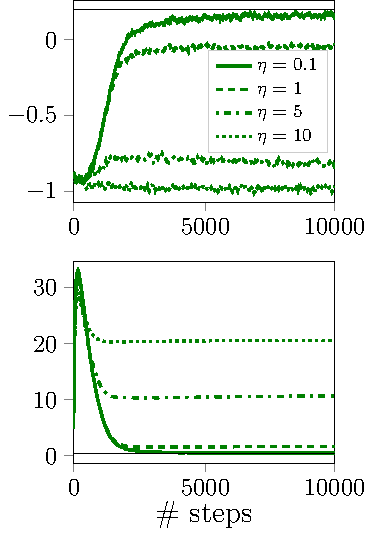
\includegraphics[scale=.7]{./imgs/gridHasseltTol/QDecWinHasselt.pdf}}
% \end{minipage}
%   \caption{Mean reward per step (top) and maximum action-value estimate in the initial state (bottom) in the Noisy Grid World problem of RQ-Learning (Figure \ref{F:hasselt_qdectol}) and windowed RQ-Learning (Figure \ref{F:hasselt_qdecwintol}) with different values of $\eta$ and $k = 0.8$. Results are averaged over $10000$ experiments.}
%   \label{F:hasselt_QDecTol}
% \end{figure}
% 
% \subsection{Double Chain}
% \begin{figure*}[t]
% \begin{minipage}{\textwidth}
% \centering
%   \subfigure[$\alpha = \dfrac{1}{n(s,a)}$\label{F:double_chain_1_1}]{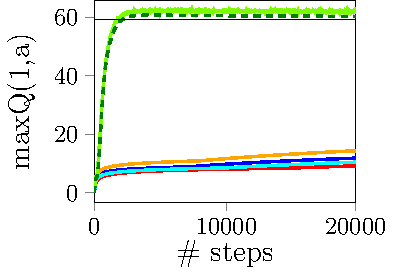
\includegraphics[scale=.7]{./imgs/doubleChain/v1-1.pdf}}
%   \subfigure[$\alpha = \dfrac{1}{n(s,a)^{0.51}}$\label{F:double_chain_1_51}]{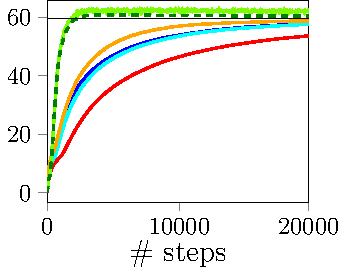
\includegraphics[scale=.7]{./imgs/doubleChain/v1-51.pdf}}
%   \subfigure[$\alpha = \dfrac{1}{n(s,a)}$\label{F:double_chain_5_1}]{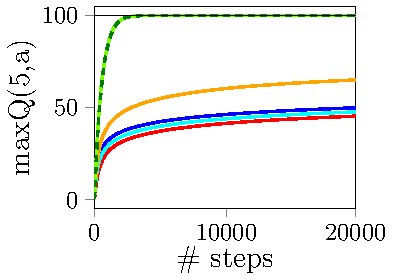
\includegraphics[scale=.7]{./imgs/doubleChain/v5-1.pdf}}
%   \subfigure[$\alpha = \dfrac{1}{n(s,a)^{0.51}}$\label{F:double_chain_5_51}]{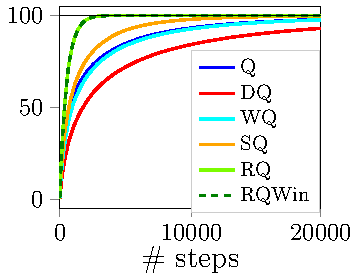
\includegraphics[scale=.7]{./imgs/doubleChain/v5-51.pdf}}
% \end{minipage}
% \caption{Maximum action-value estimate in the Double Chain problem in state $1$ (\ref{F:double_chain_1_1}, \ref{F:double_chain_1_51}) and state $5$ (\ref{F:double_chain_5_1}, \ref{F:double_chain_5_51}). Results are averaged over $500$ experiments.}
%   \label{F:double_chain_q}
% \end{figure*}
% \begin{figure*}[t]
% \begin{minipage}{\textwidth}
% \centering
%   \subfigure[$\alpha = \dfrac{1}{n(s,a)}$\label{F:lrs_1_1}]{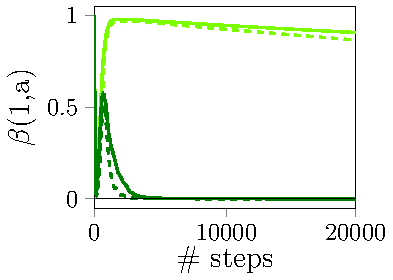
\includegraphics[scale=.7]{./imgs/doubleChain/lrs1-1.pdf}}
%   \subfigure[$\alpha = \dfrac{1}{n(s,a)^{0.51}}$\label{F:lrs_1_51}]{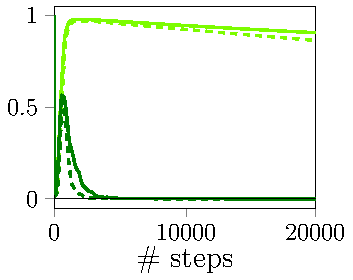
\includegraphics[scale=.7]{./imgs/doubleChain/lrs1-51.pdf}}
%   \subfigure[$\alpha = \dfrac{1}{n(s,a)}$\label{F:lrs_5_1}]{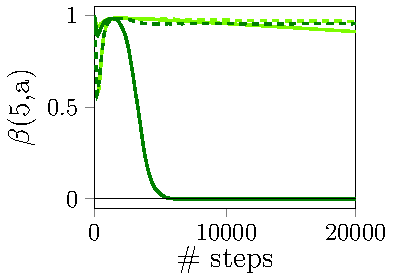
\includegraphics[scale=.7]{./imgs/doubleChain/lrs5-1.pdf}}
%   \subfigure[$\alpha = \dfrac{1}{n(s,a)^{0.51}}$\label{F:lrs_5_51}]{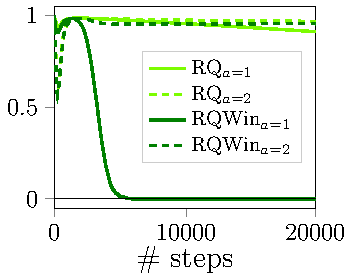
\includegraphics[scale=.7]{./imgs/doubleChain/lrs5-51.pdf}}
% \end{minipage}
% \caption{Learning rate of the two actions in the Double Chain problem in state $1$ (\ref{F:lrs_1_1}, \ref{F:lrs_1_51}) and state $5$ (\ref{F:lrs_5_1}, \ref{F:lrs_5_51}) for RQ-Learning with and without windowed variance estimation. Results are averaged over $500$ experiments.}
%   \label{F:double_chain_lr}
% \end{figure*}
% \begin{figure*}[t]
% \begin{minipage}{\textwidth}
% \centering
%   \subfigure[$\alpha = \dfrac{1}{n(s,a)}$\label{F:max_a_1}]{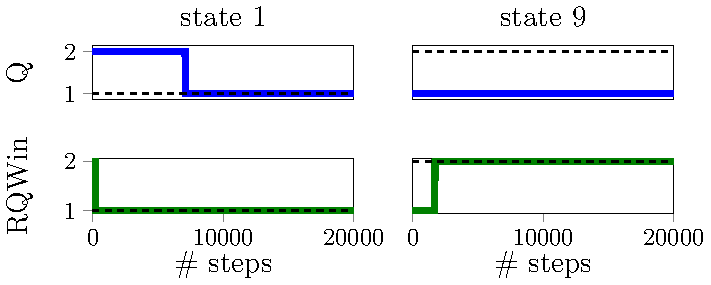
\includegraphics[scale=.7]{./imgs/doubleChain/max_a-1.pdf}}
%   \subfigure[$\alpha = \dfrac{1}{n(s,a)^{0.51}}$\label{F:max_a_51}]{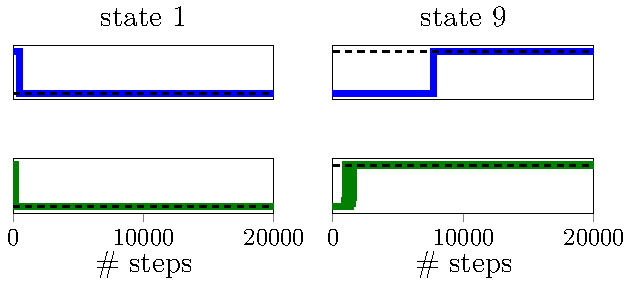
\includegraphics[scale=.7]{./imgs/doubleChain/max_a-51.pdf}}
% \end{minipage}
% \caption{Action with maximum value in the Double Chain problem in state $1$ and state $9$ for Q-Learning and windowed RQ-Learning.}
%   \label{F:max_a}
% \end{figure*}
% \begin{figure}[t]
% \begin{center}
% \begin{tikzpicture}[scale=0.11]
% \tikzstyle{every node}+=[inner sep=0pt, style={scale=0.65}]
% \draw [black] (10.4,-17.1) circle (3);
% \draw (10.4,-17.1) node {$1$};
% \draw [black] (20.1,-6.5) circle (3);
% \draw (20.1,-6.5) node {$2$};
% \draw [black] (34.4,-6.3) circle (3);
% \draw (34.4,-6.3) node {$3$};
% \draw [black] (48.2,-6.3) circle (3);
% \draw (48.2,-6.3) node {$4$};
% \draw [black] (61.6,-6.3) circle (3);
% \draw (61.6,-6.3) node {$5$};
% \draw [black] (19.4,-26) circle (3);
% \draw (19.4,-26) node {$6$};
% \draw [black] (34.4,-26) circle (3);
% \draw (34.4,-26) node {$7$};
% \draw [black] (48.2,-26) circle (3);
% \draw (48.2,-26) node {$8$};
% \draw [black] (61.6,-26) circle (3);
% \draw (61.6,-26) node {$9$};
% \draw [black] (10.195,-14.122) arc (-186.01298:-258.90993:8.628);
% \fill [black] (17.12,-6.56) -- (16.23,-6.22) -- (16.43,-7.2);
% \draw (11.87,-7.74) node [left] {$r(1)=0$};
% \draw [black] (16.449,-26.391) arc (-94.70547:-174.65436:7.013);
% \fill [black] (16.45,-26.39) -- (15.69,-25.83) -- (15.61,-26.82);
% \draw (8.26,-24.87) node [below] {$r(2)=2$};
% \draw [black] (13.375,-17.324) arc (75.15536:15.48481:8.153);
% \fill [black] (13.37,-17.32) -- (14.02,-18.01) -- (14.28,-17.05);
% \draw [black] (19.363,-9.401) arc (-21.12574:-63.79717:12.497);
% \fill [black] (13.22,-16.11) -- (14.16,-16.2) -- (13.72,-15.31);
% \draw [black] (32.152,-8.285) arc (-50.72552:-80.81899:39.653);
% \fill [black] (13.38,-16.73) -- (14.25,-17.1) -- (14.09,-16.11);
% \draw [black] (45.468,-7.539) arc (-66.30261:-81.8066:123.727);
% \fill [black] (13.37,-16.71) -- (14.24,-17.09) -- (14.09,-16.1);
% \draw [black] (58.752,-7.242) arc (-72.09117:-84.0864:221.864);
% \fill [black] (13.39,-16.81) -- (14.23,-17.23) -- (14.13,-16.23);
% \draw [black] (13.385,-17.393) arc (82.46666:56.84042:44.631);
% \fill [black] (13.39,-17.39) -- (14.11,-17.99) -- (14.24,-17);
% \draw [black] (13.394,-17.292) arc (85.54014:67.96192:107.716);
% \fill [black] (13.39,-17.29) -- (14.15,-17.85) -- (14.23,-16.86);
% \draw [black] (13.398,-17.219) arc (87.26949:73.00835:185.371);
% \fill [black] (13.4,-17.22) -- (14.17,-17.76) -- (14.22,-16.76);
% \draw (38.03,-18.9) node [above] {$r(2)=2$};
% \draw [black] (22.4,-26) -- (31.4,-26);
% \fill [black] (31.4,-26) -- (30.6,-25.5) -- (30.6,-26.5);
% \draw (26.9,-26.5) node [below] {$r(1)=0$};
% \draw [black] (37.4,-26) -- (45.2,-26);
% \fill [black] (45.2,-26) -- (44.4,-25.5) -- (44.4,-26.5);
% \draw (41.3,-26.5) node [below] {$r(1)=0$};
% \draw [black] (51.2,-26) -- (58.6,-26);
% \fill [black] (58.6,-26) -- (57.8,-25.5) -- (57.8,-26.5);
% \draw (54.9,-26.5) node [below] {$r(1)=0$};
% \draw [black] (51.2,-6.3) -- (58.6,-6.3);
% \fill [black] (58.6,-6.3) -- (57.8,-5.8) -- (57.8,-6.8);
% \draw (54.9,-5.8) node [above] {$r(1)=0$};
% \draw [black] (37.4,-6.3) -- (45.2,-6.3);
% \fill [black] (45.2,-6.3) -- (44.4,-5.8) -- (44.4,-6.8);
% \draw (41.3,-5.8) node [above] {$r(1)=0$};
% \draw [black] (23.1,-6.46) -- (31.4,-6.34);
% \fill [black] (31.4,-6.34) -- (30.59,-5.85) -- (30.61,-6.85);
% \draw (27.23,-5.85) node [above] {$r(1)=0$};
% \draw [black] (64.28,-4.977) arc (144:-144:2.25);
% \draw (68.85,-6.3) node [right] {$r(1)=10$};
% \fill [black] (64.28,-7.62) -- (64.63,-8.5) -- (65.22,-7.69);
% \draw [black] (64.117,-24.39) arc (150.34019:-137.65981:2.25);
% \draw (68.96,-25.15) node [right] {$r(1)=5$};
% \fill [black] (64.41,-27.02) -- (64.86,-27.85) -- (65.35,-26.98);
% \end{tikzpicture}
% \end{center}
% \caption{Structure of the double-chain problem.}
% \label{F:double-chain}
% \end{figure}
% This is a problem proposed in \cite{Peters2010RelativeEP}, which consists in a Markov chain with two branches (Figure \ref{F:double-chain}). In state $1$, action $1$ yields a reward of $0$ and moves the agent in state $2$; action $2$ yields a reward of $2$ and moves the agent in state $6$. In all other states, action $2$ moves the agent in state $1$ and returns a reward of $2$; action $1$ moves the agent in the next state of the chain returning a reward of $0$. In states $5$ and $9$, action $1$ yields a reward of respectively $10$ and $5$. In all states, each action has a probability of success of $0.8$ and, if the action fails, the agent remains in the current state and yields a reward of $0$. The discount factor is $\gamma = 0.9$. The optimal policy is to take action $1$ in state from $1$ to $5$ and action $2$ in the other states. RQ-Learning uses $\eta = 10$. In this experiment we focus on the estimation of the action-value function, therefore we use a fully random policy to explore the environment.
% 
% Figure \ref{F:double_chain_q} shows the estimate of the maximum action-value in state $1$ and $5$. State $5$ is the state with the highest maximum action-value. RQ-Learning approaches the optimal value faster than the other algorithms in both configurations. However, in state $1$, only RQ-Learning with windowed variance estimation converges to the optimal value because the non-windowed approach suffers from variance overestimation due to the fact that the distribution of the next action-values changes during learning; this issue, together with the stochasticity of the transitions, causes the oscillation of the estimate and slow convergence rate. This behavior is highlighted in Figure \ref{F:double_chain_lr} where we show the learning rates of the action-value in the considered states. While initially the learning rates are similar, the windowed learning rate converges to $0$, instead in the non-windowed case the learning rates decrease slowly. Note that in state $5$ the learning rate of action $2$ is almost stationary because of the complexity of the double chain structure. In this cases, increasing $\eta$ can speedup the decreasing of the learning rate.
% 
% In this experiment, RQ-Learning does not only approximate the value function very well, but it is also able to converge to the optimal policy faster than the other algorithms. Figure \ref{F:max_a} shows a comparison between Q-Learning and windowed RQ-Learning. We do not show performance of the other algorithms since they behave similarly to Q-Learning. Notice that using $k = 1$ Q-Learning and the other algorithms, except from windowed RQ-Learning, are not able to converge to the optimal policy in state $9$. Indeed, the value of action $2$ in state $9$ is the most difficult to estimate, considering the structure of the \gls{mdp}.
% 
% In this problem, where the only source of stochasticity is in the transition function, Double Q-Learning suffers the most. On the other hand, Speedy Q-Learning is still the best approach compared with the others. This empirical result confirms our conjecture.
% \subsection{Grid World with Holes}
% \begin{figure}[t]
% \begin{minipage}{\columnwidth}
% \centering
%   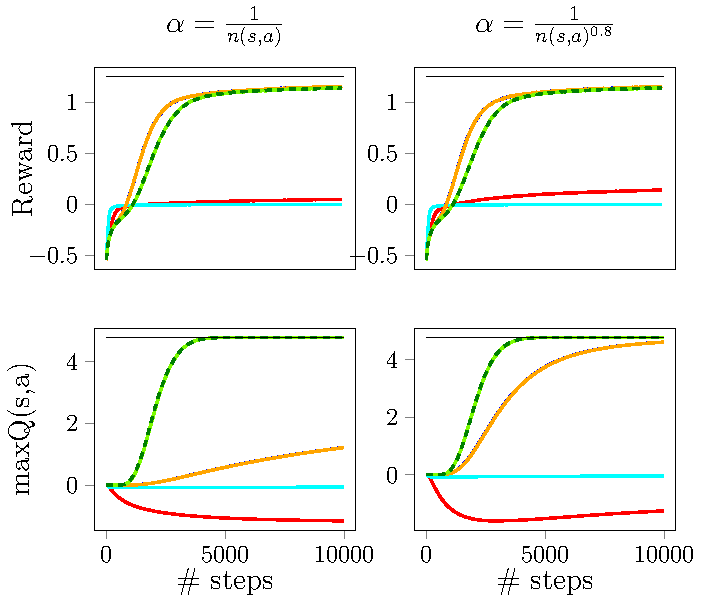
\includegraphics[scale=.7]{./imgs/gridHole/grid_hole.pdf}
% \end{minipage}
%   \caption{Mean reward per step (top) and maximum action-value estimate in the Grid World with Holes problem in the initial state (bottom) of all the other algorithms and of the best setting of RQ-Learning for this experiment. Results are averaged over $10000$ experiments.}
%   \label{F:hole}
% \end{figure}
% 
% \begin{figure}[t]
% \centering
% 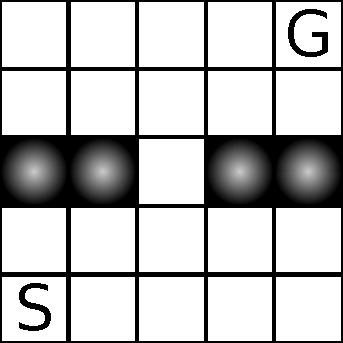
\includegraphics[scale=.55]{./imgs/gridHole/gridhole.pdf}
% \caption{Structure of the Grid World with Holes problem.}
%   \label{F:grid_hole_map}
% \end{figure}
% This environment consists in a $5 \times 5$ grid with the initial position in the lower-left cell, there are $4$ actions and the transition model is deterministic, the goal position in the upper-right cell and four holes in the middle row in such a way that only the cell in the middle is walkable (Figure \ref{F:grid_hole_map}). The agent receives a reward of $0$ in all non-hole cells, a reward of $10$ when it reaches the goal state and a reward of $-10$ when it reaches a cell with a hole. The episode ends when the agent reaches a cell with a hole or the goal state. The discount factor is $\gamma = 0.9$. RQ-Learning uses $\eta = 1$.
% The learning rate settings are the same of the previous problem.
% 
% We consider this simple problem to highlight the limitations of pessimistic action-value estimates. In this \gls{mdp} the optimal policy consists in avoiding the hole cells stepping through the state in the middle. Notice that in this state the episode terminates with negative reward with probability $\frac{\varepsilon}{2}$ due to the $\varepsilon$-greedy policy used for exploration, resulting in a very low value of the state especially at the beginning of learning. Figure \ref{F:hole} shows that while Q-Learning, Speedy Q-Learning, and RQ-Learning behave similarly well, Double Q-Learning and Weighted Q-Learning obtain very poor results due to the pessimistic estimate of the value function of the state in the middle.
% \begin{figure}[t]
% \begin{minipage}{\columnwidth}
% \centering
%   \subfigure{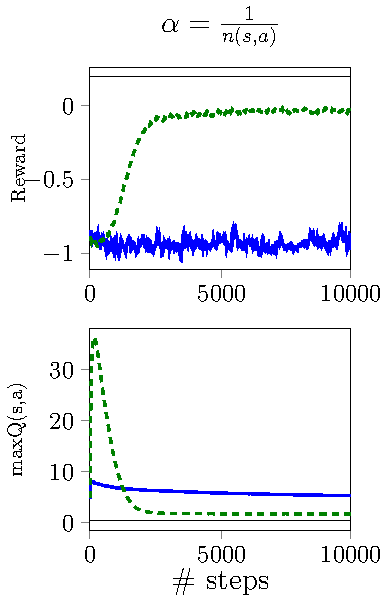
\includegraphics[scale=.7]{./imgs/sarsa/sarsa1.pdf}}\hspace{-.5cm}
%   \subfigure{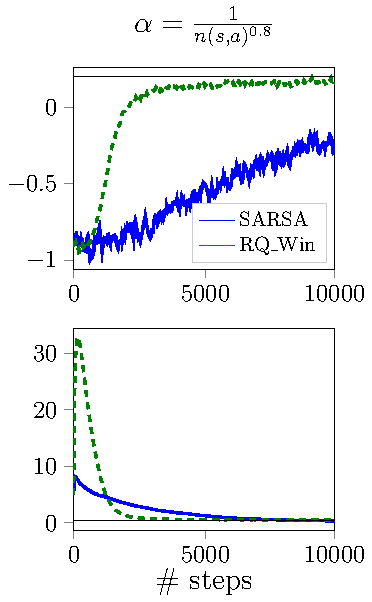
\includegraphics[scale=.7]{./imgs/sarsa/sarsa08.pdf}}
% \end{minipage}
%   \caption{Mean reward per step (top) and maximum action-value estimate in the Noisy Grid World problem in the initial state (bottom) of SARSA and of the on-policy windowed version of RQ-Learning for this experiment. Results are averaged over $1000$ experiments.}
%   \label{F:sarsa}
% \end{figure}
% 
% \subsection{On-policy learning}
% As we have discussed in the previous sections, our approach can be used also in an on-policy setting. A simple on-policy version of our algorithm can be implemented by estimating the action-value function of the current policy in the same way of the SARSA algorithm, i.e. by using the action-value function of the next action. Let $u'$ be the next action sampled by the current policy in the current state, the on-policy update is:
% \begin{align*}
% \Rtilde_{t+1}(x,u) & \leftarrow\Rtilde_t(x,u)+\alpha_t(R(x,u,x')-\Rtilde_t(x,u)),\\
% \Qtilde_{t+1}(x,u) & \leftarrow\Qtilde_t(x,u)+\beta_t(Q_t(x',u')-\Qtilde_t(x,u)).
% \end{align*}
% 
% Figure \ref{F:sarsa} compares the windowed, on-policy version of RQ-Learning with the SARSA algorithm, in the Noisy Grid World environment. It is clear that our algorithm outperforms SARSA in this \gls{mdp}.
% Since this is an on-policy setting, at each step the algorithm is estimating the current policy action-value function, not the optimal one. Indeed, by looking at the mean reward per step, our approach estimates the current action-value function of the policy better than the SARSA algorithm, i.e. the estimated action-value function is coherent with the performance of the policy.
% 
% \section{Conclusion}
% In this paper, we proposed a method to improve the learning process in stochastic \glspl{mdp} exploiting the structure of the Bellman operator. The decomposition in two components of the Bellman error allows to consider separately the sources of uncertainty. One of these components is the expected immediate reward whose uncertainty depends only on local properties of the \gls{mdp}. The other component consists in the expected value function of the next state whose uncertainty depends on the policy (in an on-line setting), on the transition model and on other action-value estimates. We showed how the proposed method obtains good results in stochastic \glspl{mdp} exploiting the information on the uncertainty of the estimates by adapting the learning rate according to it. Interestingly, this method is applicable both in off-policy and in on-policy settings; moreover, it is independent from the choice of the estimator of the expected value function of the next state.
% 
% In the experimental section, we empirically show that good results in highly stochastic \glspl{mdp} can also be reached by algorithms that overestimates the action-value function. These results demonstrate that there seems not to be such a strong correlation between the underestimation of the action-value function and good performance in these kind of environments, as suggested in recent literature. Indeed, while the propagation of overestimates could lead to divergent estimates, in some cases this is not an issue as the optimal policy only depends on the order of the action-values. Moreover, our method is able to converge to the optimal action-value even with an initially high overestimation. It demonstrates how overestimation allows a better exploration when the learning rate properly decreases. On the contrary, methods that underestimate the action-values suffer from poor exploration as we show in a simple deterministic environment.
% 
% As future work, it would be useful to derive the conditions of convergence of RQ-Learning starting from the preliminary results proposed in this paper. Moreover, it would be interesting to apply the idea of decomposing the Bellman updates, and exploiting uncertainty of its components, to continuous space problems and other types of learning settings (e.g. batch). Finally, it would be interesting to evaluate whether Deep Reinforcement Learning algorithms could benefit from the introduction of our framework.

\part{Uncertainty-Driven Exploration}
\chapter{Exploration}

\chapter{Exploration Driven by an Optimistic Bellman Equation}\label{C:opt}
As described in Chapter~\ref{C:ts}, the \gls{ofu}-based techniques encourage exploration of unknown states hoping that they are more convenient than already known ones, thus the definition of optimism. There are two kinds of optimism:
\begin{itemize}
\item \textbf{confidence interval estimation}, such as IEQL+~\cite{meuleau1999exploration} and UCRL~\cite{auer2007logarithmic}, which directly estimates $Q$-value confidence intervals;
 \item \textbf{optimistic estimate} of the action-value, a method proposed for instance in~\cite{sutton1998reinforcement} about which subsequently~\cite{even2002convergence} proved convergence to a near-optimal solution.
\end{itemize}
While the work in Chapter~\ref{C:ts} deals with the first category of optimism-based algorithms, the work described in the following deals with the second one. This approach is inspired by the broad category of algorithms based on \gls{im}~\cite{singh2004intrinsically}, that despite having less theoretical guarantees
than Bayesian approaches, have been able to obtain impressive results~\cite{bellemare2016unifying}. As already discussed in Chapter~\ref{C:ts}, \gls{im}
algorithms define an additional \textit{intrinsic} reward, which acts as an exploration bonus. Often, the additional reward is defined using heuristics, such as counting state visits and rewarding less visited states~\cite{ostrovski2017count}, or by \textit{surprise} which is the error in predicting future states~\cite{pathak2017curiosity}. However, the drawback of \gls{im} techniques is their lack of a principled definition of the intrinsic reward for exploration.

Considering this premise, we worked on the proposal of the \gls{obe}, a novel variant of \gls{be} which results in an optimistic action-value estimate
from an ensemble of action-value functions where the optimistic estimate is obtained from a maximum-entropy principle. For the exploration bonus that \gls{obe} implicitly defines, we can prove that the bonus decreases consistently with the number of
state visits. Our proposed algorithm can be seen as a mixture of
different techniques: as an approximated Bayesian method~\cite{engel2005reinforcement,vlassis2012bayesian} we estimate
the uncertainty with an ensemble~\cite{osband2017deep}; like optimism-based methods~\cite{lai1985asymptotically,kearns2002near,brafman2002r,azizzadenesheli2517efficient} we select
optimistic estimates, and like \gls{im} we propagate an implicit
exploration bonus~\cite{singh2004intrinsically,schmidhuber2008driven,white2010interval}.

\section{Learning value function ensembles with optimistic estimate selection}
\label{sec:obe}
Ensemble methods~\cite{opitz1999popular} constitutes a popular set of \gls{ml} technique where multiple models are used to learn the same target function. In addition to being commonly used to improve the generalization of the prediction, ensemble methods offer a simple way to estimate its uncertainty. We consider the application of ensemble methods in the \gls{rl} framework with the purpose of approximating the action-value functions while having an estimate of their uncertainty, in order to apply the \gls{ofu} principle in action selection.

\subsection{An optimistic Bellman equation for action-value function ensembles}
Starting from the purpose of overestimating the action-value functions with the result of encouraging exploration, we propose \gls{obe} which propagates an optimistic estimate of the action-value function. In particular, \gls{obe} is a \gls{be} which incorporates the information about the uncertainty provided by a action-value function ensemble. We want to emphasize that, when all the action-value functions of the ensemble are identical, we assume that there is no uncertainty and under this condition the \gls{obe} will behave exactly equivalently to the classic \gls{be}. Indeed, we can prove that the fixed point $Q^*$ of \gls{obe} is the same of the classic \gls{be}; in other words, the \gls{obe} differs from the classic \gls{be} when the estimates in the ensemble are different among themselves, which usually happen when the action-value functions are approximated with a limited number of samples or with function approximators (e.g. neural networks). This makes sense, since when the perfect solution is available there is no need for optimism and exploration. 
Note that the fact that \gls{obe} enjoys the properties of the classical \gls{be}, like contractivity and the existence of a unique fixed point, potentially enables its usage in value-based and actor-critic algorithms.

The diversity in the action-value ensemble should be ideally consistent with the uncertainty of the estimation: when the estimate is certain, all the values in the ensemble should agree on the same value, otherwise the ensemble should have discordant values.
Given an ensemble of action-value functions $\{Q_m\}_{m=1}^M$, we want to work out an optimistic estimate from the diverse estimates provided by the ensemble. The simplest and most optimistic solution is to select the highest value
\begin{equation}
 \max_m Q_m(s,a).
\end{equation}
However selecting the highest estimate makes poor use of the information provided by the ensemble and can be sensible to noise. In order to mitigate this effect, we introduce a notion of \textit{belief} over the estimates where $b_m(s,a)$ is the belief of $Q_m(s,a)$. The main idea is to add an entropic regularization term to the objective
\begin{equation}
 \max_{b(s,a)} \sum_m b_m(s,a) Q_m(s,a) - c \sum_{m} b_m \log b_m
\end{equation}
or to bound the information loss
\begin{equation}
\sum_m b_m \log b_m < \psi.
\end{equation}
Hard constraint on the information loss is more appealing since the introduced hyper-parameter $\psi$ does not depend on the magnitude of the rewards but has no closed-form solution. In contrast, the penalization weighting constant $c$ introduced by the soft-constraint regularization term is sensitive to the magnitude of the rewards, but admits a closed-form solution.
Basing on these considerations, we define two different problems where we use an optimistic estimate of the action-value function.

\subsubsection{Entropy-regularized optimistic action-value selection}
We define a \gls{be} over the action-value function ensemble by introducing an optimistic estimate penalized by an entropic regularization term.
\begin{probdef}[Regularized version]
\begin{equation}
\arraycolsep=1.4pt\def\arraystretch{2.2}
\begin{array}{rrclcl}
\displaystyle Q_i(s,a) = \max_{b(s,a) \in \mathcal{P}^M} & \multicolumn{3}{l}{R(s,a) + \gamma \sum_m{b}_m(s,a)V_m'(s,a)-\frac{1}{\eta}D_{\mathrm{KL}}\big(b_m(s,a)\big{\|}u\big) } \\
\textrm{s.t.} & \sum_{m=1}^{M} b_m(s,a) & = & 1 \\
\multicolumn{4}{l}{ \forall s,a,i \in \mathcal{S} \times \mathcal{A} \times \{1,\dots,M\}}
\end{array}\nonumber
\end{equation}\label{PROB:regularized}
\end{probdef}
\noindent with $u_m  =  \nicefrac{1}{M}$, $D_{KL}(b(s,a)\| u)$ is the \gls{kl} divergence between the belief $b(s,a)$ and the uniform distribution $u$, and $V_m'(s,a) \! = \! \sum_{s'} P(s'|s,a)\max_{a'}Q_m(s',a')$.
The choice of using the relative entropy (i.e. \gls{kl}-divergence) instead of the absolute one has two main advantages: it admits a solution for $\eta \to 0$ and provides a normalization factor.
Since Problem~\ref{PROB:regularized} is a convex constrained problem, it is solvable by dual optimization. Introducing $\lambda$ as Lagrangian multiplier for the constraint, we write the Lagrangian
\begin{eqnarray}
L_i(s,a) \!&=& \!f(s,a; b(s,a)) -\frac{1}{\eta}D_{\mathrm{KL}}\big(b(s,a)\big{\|}u\big)\nonumber \\ && + \lambda\bigg(\sum_m b_m(s,a) - 1\bigg).\label{E:lagrangian}
\end{eqnarray}
Requiring the partial derivatives of $L_i$ w.r.t $p_m$ and $\lambda$ to be zero yields 
\begin{equation}
b_m(s,a) = \frac{e^{\eta  \gamma V_m'(s,a)}}{\sum_{k=1}^{M} e^{\eta \gamma   V_k'(s,a)}}\label{pm}.
\end{equation} 
By substituting $b_m$ in Equation~\ref{E:lagrangian}, we obtain the solution to the problem:
\begin{equation}
Q_i(s,a) = \begin{cases}
\overline{R}(s,a) + \frac{1}{\eta} \log \frac{\sum_{m=1}^Me^{\eta \gamma  V_m'(s,a) }}{M} & \mathrm{if} \eta \neq 0 \label{OBE} \\
\overline{R}(s,a) + \frac{\gamma}M \sum_{m=1}^{M} V_m'(s,a) & \mathrm{otherwise}
\end{cases}.
\end{equation}
Notice that $\eta>0$ leads to a positive (optimistic) biased estimation, while $\eta<0$ will leads to a negative (pessimistic) estimate; in this work we will always assume $\eta>0$ (and therefore we refer to the equation as optimistic). 
However, in general, the choice of $\eta$ is difficult since it depends on the magnitude of the reward function. For this reason we introduce the constrained version of the proposed problem.
 
\subsubsection{Optimistic action-value selection bounding the information loss}
We bound the information loss between the distribution $b_m$ and the uniform distribution to maintain compatibility with Problem~\ref{PROB:regularized}. The information loss is bounded between $-\log M$ and $0$ where  $-\log M$ stands for complete information loss (i.e., only one model is selected) while $0$ corresponds to no information loss (i.e., uniform belief distribution). Constraining the information loss has succeeded in prior work, for instance in policy search methods such as~\cite{peters2010relative}.
\begin{probdef}[Constrained version]
\begin{equation}
\begin{array}{rrclcl}
\displaystyle Q_i(s,a) = \max_{b(s,a) \in \mathcal{P}^M} & \multicolumn{3}{l}{R(s,a) + \gamma \sum_m{b}_m(s,a)V_m'(s,a)\nonumber } \\
\text{s.t.} & D_{\mathrm{KL}}\big(b(s,a)\big{\|} u \big)& \leq & \iota_{\max} \\
& \sum_{m=1}^{M} b_m(s,a) & = & 1 \\
\multicolumn{4}{l}{ \forall s,a,i \in \mathcal{S} \times \mathcal{A} \times \{1,\dots,M\}}
\end{array} \nonumber
\end{equation}\label{PROB:constrversion}
\end{probdef}
\noindent By letting $\beta$ be the Lagrangian multiplier associated with the KL constraint, we obtain the Lagrangian
\begin{eqnarray}
L_i &\! = \!& f(s,a;b(s,a)) + \beta (D_{\mathrm{KL}}(b(s,a){\|}u) - \iota_{\max}) \nonumber \\
& &   + \lambda(\sum_m b_m(s,a) - 1).\label{E:lagrangian2}
\end{eqnarray}
Substituting $\beta$ with $\nicefrac{-1}{\eta}$ we note that Equation~\ref{E:lagrangian2} becomes identical to~\ref{E:lagrangian} except for a constant factor. Since we can not solve $\eta$ (or $\beta$) analytically, we obtain an approximate solution by iteratively optimizing $\eta$ (or $\beta$) and $b_m$ subsequently.
\gls{obe} takes its name from the fact that when $\eta > 0$, the \textit{logsumexp} acts as a softmax operator. Such operator is also well known as an \textit{entropic mapping}, as it can be derived from a maximum-entropy principle.

The use of the entropic mapping is not new in \gls{rl}: \cite{pmlr-v70-asadi17a} propose an interesting use of the entropic mapping as a soft-max over the action in the \gls{be}; \cite{peters2010relative} instead obtain it from an entropic regularization over the state-action distribution.

\subsection{Relation to Intrinsic Motivation}
In order to highlight the connection between \gls{obe} and \gls{im}, we reformulate \gls{obe} utilizing the unbiased average of the estimates instead of the logsumexp, and by introducing the resulting exploratory bonus $U$ which includes the positive bias
\begin{eqnarray}
Q_i(s,a)\! &=&\! \overline{R}(s,a) + U(s,a) +  \gamma  \sum_{m=1}^M \frac{V_m'(s,a)}{M} \label{bonusBE}
\end{eqnarray}
with
\begin{equation}
U(s,a) \! =\!  \frac{1}{\eta}\log\sum_{m=1}^M \frac{e^{\eta\gamma V_m'(s,a)}}{M} - \gamma  \sum_{m=1}^M \frac{V_m'(s,a)}{M}. \label{bonusdef}
\end{equation}
Noticing that $\dfrac{\sum_{i=1}^N e^{\eta x_i}}{N}$ is the \textit{sample moment generator} w.r.t. samples $\{x_i\}_{i=1}^N$ we can rephrase the exploration bonus as
\begin{eqnarray}
U(s,a)& = & \lim_{N \to +\infty}\frac{1}{\eta} \log [  1 + \sum_{n=2}^{N} \frac{(\eta\gamma)^n}{n!}\mathcal{M}_n(s,a)] \nonumber \\
& = & \eta \gamma \mathcal{M}_2(s,a)  + O(\eta^2)\label{bonus}
\end{eqnarray}
where $\mathcal{M}_n$ is the $n$\textsuperscript{th} central moment of the random variable $V_m'$
\begin{equation}
\mathcal{M}_n(s,a) = M^{-1} \sum_{m=1}^M [( V_m'(s,a) -\overline{V}(s,a))^n]\nonumber
\end{equation}
with 
\begin{equation}
\overline{V}(s,a) = M^{-1} \sum_{m=1}^M V_m'(s,a).\nonumber
\end{equation}
Equation \eqref{bonusBE} shows that \gls{obe} is equivalent to \gls{be} with an additional bonus defined by Equation~\ref{bonus}. The bonus $U$ (for any positive $\eta$) is always positive, and provides a measure of the uncertainty w.r.t. $Q$. This is why \gls{obe} can be interpreted as a special principled form of \gls{im}.

\subsubsection{Explicit exploration} A general problem affecting \gls{im} algorithms, is that the policy greedy to the obtained action-value function, is not optimized for the original problem. As a solution to this issue we approximate two functions: $\tilde{Q}$, which will be updated using the true reward and $Q_E$ which will be updated using only the intrinsic reward \cite{szita2008many}. In this way we obtain both the \gls{im} policy $\pi_o(s) = \arg \max_{a} \tilde{Q}(s,a) + Q_E(s,a)$ and the classic policy  $\pi_u(s) = \arg \max_{a} \tilde{Q}(s,a)$.
Define 
\begin{eqnarray}
	\tilde{Q}_i(s,a) = R(s,a) + \gamma \sum_{m=1}^M\frac{\tilde{V}_m'(s,a)}{M} \quad \text{with} \\
	\tilde{V}_m'(s,a) =  \sum_{s'} P(s'|s,a)\max_{a'}\tilde{Q}_m(s',a')
\end{eqnarray}
to obtain an unbiased estimate of the action-value function, yielding
\begin{eqnarray}
Q_E(s,a) & = & \sum_{t=0}^T \gamma^t U(s_t,a_t) \quad \text{where} \quad s_0 = s, a_0 = a \nonumber \\
& = & \eta^{-1}\log \frac{\sum_{k=1}^M e^{\eta\gamma\max_{a'}\tilde{Q}_k(s',a') + Q_E(s',a')}}{M}\nonumber \\
& &  -  \frac{\sum_{k=1}^M \gamma\max_{a'}\tilde{Q}_k(s',a')}{M}.
\end{eqnarray}
By a simple equation rearrangement, it is possible to show that $\tilde{Q}_i(s,a) + Q_E(s,a)$ is equivalent to $Q_i(s,a)$ as defined in the \gls{obe}~\ref{OBE}.
 
\section{Optimistic value function estimators}
The \gls{obe} offers a theoretical framework in which it is possible to develop optimistic value based algorithms. In fact, \gls{obe} enjoys all the desirable properties of the \gls{be} (e.g. max-norm contractivity). We present briefly two practical applications of the OBE that are optimistic variants of $Q$-learning and \gls{dqn} that we call, respectively, \gls{oql} and \gls{odqn}.
\subsection{Optimistic $Q$-Learning}
Motivated by the idea of employing an ensemble of regressors as is done in \gls{bdqn}~\cite{osband2017deep}, we assume to have $M$ randomly initialized $Q$-tables. Inspired by the well known $Q$-learning update rule~\ref{S:Q-Learning}, we derive an optimistic version which is consistent with the \gls{obe} as follows:
\begin{align*}
      \small  Q_{i, t+1}(s,a) &= (1-\alpha_t)Q_{i,t}(s,a)  \nonumber  \\
  & \small + \alpha_t (r_t + \frac{1}{\eta} \log M^{-1} \sum_{j=1}^M e^{\gamma \max_{a'} Q{j,t}(s', a')}).\nonumber
\end{align*}
\label{def:optimistic_qlearning}
We show that, with the update rule proposed, given infinite visits of each state-action pair, all the tables will converge to the same values, and more precisely, after each update, the $n$-th central moment of the updated cell is scaled exactly by $(1 - \alpha_t)^n$:
\begin{equation}
 \mathcal{M}_{n,t+1}(s,a) = (1-\alpha_t)^n \mathcal{M}_{n,t}(s,a) \label{momentdecreasing}
\end{equation}
where 
\begin{equation}
 \mathcal{M}_{n,t}(s,a) = M^{-1} \sum_{i=1}^M (Q_{i,t}(s,a) - \sum_{k=1}^M \frac{Q_{k,t}(s,a)}{M})^n. \nonumber
\end{equation}
This implies that a cell updated $N$ times, with learning rates $\{\alpha_i\}$, will have the $n$-th central moments scaled by $\Pi_{\alpha_i}(1-\alpha_i)^n$ w.r.t.\ the initial one. This leads us to some considerations:
\begin{enumerate}
 \item the bonus decreases accordingly to the number of state visits;
 \item differing from several count-based approaches, our algorithm takes into account the impact of the learning rate;
 \item in the limit of an infinite number of visits, the exploration bonus converges to $0$.
\end{enumerate}
All the considerations done so far provide a deeper insight about how the algorithm works and its properties. However, in a more complex settings, (e.g., function approximation) the convergence to $0$ of the exploration bonus is not guaranteed in general.

\subsection{Optimistic Deep $Q$-Network}\label{sec:proposedalg}
In addition to the novel \gls{oql} algorithm described previously which can be used for limited discrete state spaces, we
propose another algorithm for continuous state spaces based on our \gls{obe} taking inspiration from the framework provided by \gls{bdqn}~\cite{osband2017deep}
which uses an ensemble of neural networks to estimate the action-value function.
To get an unbiased performance evaluation, we decided to update $M-1$ components of the ensemble with the update rule provided by \gls{bdqn} and to use the remaining $M$-th component of the ensemble to approximate $Q_E$. Using the first component to approximate $Q_E$, we get for our new algorithm \gls{odqn} the loss
\begin{eqnarray}
	&\mathcal{L}_O(s,a) = (\eta^{-1}\log \frac{\sum_{k=2}^M
	 e^{\eta\gamma\max_{a'}Q_k^T(s',a')+ Q_1^T(s',a')}}{M}\nonumber \\
&\qquad\qquad\;\;\;\;  -  \frac{\sum_{k=2}^M  \gamma\max_{a'}Q^T_k(s',a')}{M} -Q_1(s,a))^2\nonumber \\
&\;  + \sum_{k=2}^M (r + \gamma\max_{a'}Q^T_k(s',a') -
	 Q_k(s,a))^2.  \label{optimisticloss}
\end{eqnarray}
The exploratory bonus represented by $Q_E = Q_1$ in the proposed \gls{oql} and \gls{odqn} algorithms is needed to
guide exploration during learning. During evaluation, we use majority voting on the remaining $M-1$
components $\{Q_k\}_{k=2}^M$. While we always select an optimistic policy in \gls{oql} during the training phase, in
\gls{odqn} the neural network function approximator may have problems learning to approximate the optimal
policy: if there are not enough unbiased samples the approximator may learn to model only the optimistic
biased samples. Note that in the tabular case, this is not a problem since there is no action-value function
approximation. In order to mitigate this problem, we introduce a hyper-parameter $\chi$ which denotes the probability to select an optimistic policy $\pi_o$ in place of the unbiased one $\pi_u$. In this way, we can balance the number of unbiased and optimistic samples.
Algorithm \ref{optimisticdqn} shows the pseudocode of \gls{odqn}. 
\begin{algorithm}[t]
	\caption{Optimistic Deep $Q$-Network}
	\label{optimisticdqn}
	\begin{algorithmic}
		\STATE \textbf{Input:} $\{Q_k\}_{k=1}^K$, $\iota_{\max}$, $\eta_{\mathrm{init}}$, $\chi$, $N$, $C$
		\STATE Let $B$ be a replay buffer storing the experience for training.
		\STATE $\eta = \eta_{\mathrm{init}}$.
		\STATE Let $i \sim \mathrm{Uniform}\{1 \dots M\}$ and $\psi = 1$ w.p. $\chi$ otherwise $\psi = 0$
		\FOR{$N$ epochs}
		\FOR{$C$ steps}
		\STATE Observe $s$
		\STATE Choose $a = \arg \max_a Q_i(s,a) + \psi Q_1(s,a)$
		\STATE Observe reward $r$, next state $s'$, end of episode $t$
		\STATE If $t$ is terminal, $i \sim \mathrm{Uniform}\{2 \dots M\}$ and \\ \ \ \ \ \ \ $\psi = 1$ w.p. $\chi$ otherwise $\psi=0$
		\STATE Store $<s,a,r,s',t>$ in buffer $B$
		\STATE Sample mini-batch $B_{\mathrm{batch}}$
		\STATE Update $\{Q_k\}_{k=1}^K$ using equation \eqref{optimisticloss}
		\STATE $V \leftarrow V + |$ violated constraints \eqref{batchconstr} in $B_{\mathrm{batch}}|$ 
		\ENDFOR
		\STATE Let $\rho = \frac{V}{C * \mathrm{batch\_size}}$
		\STATE Update $\eta$ by \eqref{etaupdate}
		\STATE Update target network
		\ENDFOR
	\end{algorithmic}
\end{algorithm}

\paragraph{Automatic hyper-parameter adaptation}
\label{subsec:adaptive}
Recalling that the regularization coefficient $\eta$ in the \gls{obe} is hard to tune, we want to focus our attention on Problem~\ref{PROB:constrversion}. We propose a way, inspired by~\cite{schulman2017proximal}, to optimize $\eta$.
One of the optimization techniques proposed in this work is to measure the ``degree'' of constraint violation and to update the Lagrangian multiplier accordingly. We have to adapt the technique to multiple constraints, as the problem is defined for each state-action pair: we count the number of times the constraints have been violated and then update $\eta$. In more detail, suppose to have $N$ state-action pairs and for each pair $(s_i, a_i)$
\begin{eqnarray}
\sum_m b_m(s_i,a_i) (\log b_m(s_i,a_i) + \log M) \leq \iota_{\max}, \label{batchconstr}
\end{eqnarray}
where $\iota_{\max}$ is defined in Problem~\ref{PROB:constrversion}, while $b_m(s_i,a_i)$ is defined by \eqref{pm}. We define $\rho$ as the ratio of violated constraints. We update $\eta$ according to the following rule
\begin{equation}
\eta_{T+1} = \frac{\eta_{T}}{(0.5 +  10 \rho)} \label{etaupdate}.
\end{equation}
In \gls{odqn}, we decided to count the number of constraints violated every $C$ time-steps (basically every update of the target network), using the samples of all the extracted mini-batches. See Algorithm~\ref{optimisticdqn} for further details. 
  
\paragraph{Ensuring a prior distribution} As already discussed, it is important to maintain diversity in our ensemble, and this diversity should reflect the degree of uncertainty. For this reason, we should introduce a sort of prior distribution, as happens in the Bayesian framework. In the case of \gls{oql}, we observe that it is sufficient to randomly initialize each element of the ensemble, since diversity between estimates is a sufficient condition to obtain positive bonus.
For \gls{odqn}, as is done in \gls{bdqn}, we choose to maintain the diversity between approximation, by a random initialization of each component parameters.

\section{Experimental evaluation}
\label{S:odqn_experiments}
In the experiments, we compare \gls{oql} with a tabular variant of \gls{bdqn} which we call \gls{bql}, classical $Q$-learning and \gls{oiql}~\cite{sutton1998reinforcement}; on the other hand we preliminarily evaluate \gls{odqn} method with \gls{bdqn} and classical \gls{dqn} in a simple problem.

\subsection{Settings}
The environments are chosen to cover different types of dynamics and having sparse rewards: they are Frozen Lake as implemented in~\cite{gym}, Taxi as presented in Chapter~\ref{C:ts} and the chain in Figure~\ref{F:chain}.

\begin{figure*}[t]
  \centering
  \begin{tikzpicture}[scale=1, transform shape]
  \node[state]             (1) {1};
  \node[state, right=of 1] (2) {2};
  \node[state, right=of 2] (3) {\dots};
  \node[state, right=of 3] (4) {N};
  \draw[every loop]
  (1) edge[loop above] node {b, $0.001$} (1)
  (1) edge[bend left, auto=left] node {a} (2)
  %(2) edge[loop above] node {a} (2)
  (2) edge[bend left, auto=left] node {a} (3)
  %(3) edge[loop above] node {a} (3)
  (3) edge[bend left, auto=left] node {a} (4)
  %(1) edge[loop below] node {b} (1)
  (2) edge[bend left, auto=left] node {b} (1)
  %(2) edge[loop below] node {b} (2)
  (3) edge[bend left, auto=left] node {b} (2)
  %(3) edge[loop below] node {b, $1$} (3);
  (4) edge[bend left, auto=left] node {b} (3)
  (4) edge[loop above] node {a, $1$} (4);
  \end{tikzpicture}\caption{Structure of the Chain.}\label{F:chain}
\end{figure*}

\paragraph{Initialization of the action-value function} In the tabular setting, for \gls{oiql} we initialize the action-value function to $15$ in Taxi and to $1$ in Chain and Frozen Lake. For the other algorithms, we initialize $Q(s,a) \sim \mathcal{N}(\mu=0,\sigma=2)$, except $Q_E$ of \gls{oql} is initialized to $0$.
In the taxi environment, we use a shared convolutional layer with multiple heads as described in \cite{osband2017deep}. In the case of \gls{odqn} we initialize the output layer corresponding to $Q_E$ to small values of the parameters, in order to obtain initially $Q_E \approx 0$. 

\paragraph{Hyper-parameters tuning} For the tabular settings, we did not run any hyper-parameter optimization. With neural networks we compare \gls{odqn} and \gls{bdqn} using the best hyper-parameter setup found for \gls{bdqn}. In \gls{oql} we use $\eta=10$ and for \gls{odqn}, we use $\chi=0.25$ and $\iota_{\max}=1$.

\setlength\figureheight{4cm}
\setlength\figurewidth{4cm}
\begin{figure*}[t]
	% This file was created by matplotlib2tikz v0.6.18.
\begin{tikzpicture}

\definecolor{color0}{rgb}{0.12156862745098,0.466666666666667,0.705882352941177}
\definecolor{color1}{rgb}{1,0.498039215686275,0.0549019607843137}
\definecolor{color2}{rgb}{0.172549019607843,0.627450980392157,0.172549019607843}
\definecolor{color3}{rgb}{0.83921568627451,0.152941176470588,0.156862745098039}
\definecolor{color4}{rgb}{0.549019607843137,0.337254901960784,0.294117647058824}
\definecolor{color5}{rgb}{0.890196078431372,0.466666666666667,0.76078431372549}

\begin{groupplot}[group style={group size=4 by 2}]
\nextgroupplot[
height=\figureheight,
tick align=outside,
tick pos=left,
title={50-Chain},
title style={font=\small, yshift=-1.5ex},
xlabel style={font=\scriptsize},
yticklabel style={font=\scriptsize},
xticklabel style={font=\scriptsize},
grid=both,
width=\figurewidth,
x grid style={white!69.01960784313725!black},
xmin=-14.95, xmax=313.95,
y grid style={white!69.01960784313725!black},
ymin=-0.618016756356909, ymax=10.6593649530358
]
\path [fill=color0, fill opacity=0.3] (axis cs:0,0.00823092684258694)
--(axis cs:0,0.0191220143338837)
--(axis cs:1,0.0146868972189267)
--(axis cs:2,0.0161087413567854)
--(axis cs:3,0.0176472840019849)
--(axis cs:4,0.0249082448559281)
--(axis cs:5,0.026376326086257)
--(axis cs:6,0.0287891093301067)
--(axis cs:7,0.0284939685639376)
--(axis cs:8,0.0249156509494596)
--(axis cs:9,0.0309062507427155)
--(axis cs:10,0.0255619512105429)
--(axis cs:11,0.022384516846227)
--(axis cs:12,0.0215650269443974)
--(axis cs:13,0.0182076082981445)
--(axis cs:14,0.0181649810611131)
--(axis cs:15,0.019350550033596)
--(axis cs:16,0.017523547360708)
--(axis cs:17,0.0239144890778476)
--(axis cs:18,0.0205246158253211)
--(axis cs:19,0.021783704911025)
--(axis cs:20,0.0162951225630373)
--(axis cs:21,0.0221030107288587)
--(axis cs:22,0.0219878001488333)
--(axis cs:23,0.0165610164967063)
--(axis cs:24,0.0231463356829901)
--(axis cs:25,0.0251815647686646)
--(axis cs:26,0.0174170274179694)
--(axis cs:27,0.0150828793432824)
--(axis cs:28,0.0140076872054926)
--(axis cs:29,0.0150947419541605)
--(axis cs:30,0.0246753172560022)
--(axis cs:31,0.0149404571265054)
--(axis cs:32,0.0143934636518426)
--(axis cs:33,0.0169578737153203)
--(axis cs:34,0.0171669724200997)
--(axis cs:35,0.0192906721050006)
--(axis cs:36,0.018973880896521)
--(axis cs:37,0.0191732556685254)
--(axis cs:38,0.0169468641346492)
--(axis cs:39,0.0210951737020129)
--(axis cs:40,0.0143501374386799)
--(axis cs:41,0.0197373171037569)
--(axis cs:42,0.0121056359941294)
--(axis cs:43,0.0140442183437932)
--(axis cs:44,0.0159555134523136)
--(axis cs:45,0.0173941084893068)
--(axis cs:46,0.0163579338134927)
--(axis cs:47,0.0154442374869428)
--(axis cs:48,0.0119977016129309)
--(axis cs:49,0.0157137570190656)
--(axis cs:50,0.0143805776930276)
--(axis cs:51,0.0114636873661823)
--(axis cs:52,0.0136742173982719)
--(axis cs:53,0.00986221514669076)
--(axis cs:54,0.0114975730770707)
--(axis cs:55,0.0139151843324922)
--(axis cs:56,0.0195267701033303)
--(axis cs:57,0.0144733426766197)
--(axis cs:58,0.0100741660128398)
--(axis cs:59,0.0136020335454657)
--(axis cs:60,0.0130678497649668)
--(axis cs:61,0.0210320259278234)
--(axis cs:62,0.0155212611951926)
--(axis cs:63,0.0112954331480545)
--(axis cs:64,0.00760327546025448)
--(axis cs:65,0.0129712736459636)
--(axis cs:66,0.00879525283831337)
--(axis cs:67,0.0119214768110086)
--(axis cs:68,0.00977351062666433)
--(axis cs:69,0.00994959429595321)
--(axis cs:70,0.0104262800764816)
--(axis cs:71,0.00569823937821569)
--(axis cs:72,0.0112872462653019)
--(axis cs:73,0.00889369660400013)
--(axis cs:74,0.00602202968260877)
--(axis cs:75,0.00961544550070766)
--(axis cs:76,0.00619397825267707)
--(axis cs:77,0.0130960171424155)
--(axis cs:78,0.0114573967608302)
--(axis cs:79,0.00569006291232065)
--(axis cs:80,0.0112362740736754)
--(axis cs:81,0.0067612436429803)
--(axis cs:82,0.00492546296098201)
--(axis cs:83,0.0104728316144554)
--(axis cs:84,0.0115691584505391)
--(axis cs:85,0.0108453502275619)
--(axis cs:86,0.0104830377439265)
--(axis cs:87,0.00702905130837173)
--(axis cs:88,0.00873767903590831)
--(axis cs:89,0.00523658631531032)
--(axis cs:90,0.0110755709068476)
--(axis cs:91,0.0119983250096664)
--(axis cs:92,0.0111311316364887)
--(axis cs:93,0.00732282986191366)
--(axis cs:94,0.00757296283695606)
--(axis cs:95,0.0108368021323785)
--(axis cs:96,0.0056513952107335)
--(axis cs:97,0.00838232850169643)
--(axis cs:98,0.00924798308206145)
--(axis cs:99,0.0135235089894456)
--(axis cs:100,0.00928289445740305)
--(axis cs:101,0.00700876096927406)
--(axis cs:102,0.00764281680414605)
--(axis cs:103,0.00609961908787784)
--(axis cs:104,0.00744142864410255)
--(axis cs:105,0.00938988938827763)
--(axis cs:106,0.00869450553749319)
--(axis cs:107,0.00675649349647292)
--(axis cs:108,0.0054550284522141)
--(axis cs:109,0.00779470745841356)
--(axis cs:110,0.00831526108242772)
--(axis cs:111,0.00713620835375248)
--(axis cs:112,0.00886390580128766)
--(axis cs:113,0.00896175244298851)
--(axis cs:114,0.0108612127008784)
--(axis cs:115,0.00487676701913783)
--(axis cs:116,0.00487837930224114)
--(axis cs:117,0.00660171501368254)
--(axis cs:118,0.00348465572858743)
--(axis cs:119,0.194481042986987)
--(axis cs:120,0.026156473126586)
--(axis cs:121,0.110373385766031)
--(axis cs:122,0.00810021538752208)
--(axis cs:123,0.0838242397773776)
--(axis cs:124,0.16105960989288)
--(axis cs:125,0.398067686401346)
--(axis cs:126,0.638376040021761)
--(axis cs:127,0.823541173464604)
--(axis cs:128,0.923698458151547)
--(axis cs:129,1.11648660457872)
--(axis cs:130,0.941197152698387)
--(axis cs:131,1.13947399042241)
--(axis cs:132,1.24147256203967)
--(axis cs:133,1.80540713019755)
--(axis cs:134,1.67453809991011)
--(axis cs:135,1.61386070885513)
--(axis cs:136,1.69081434948269)
--(axis cs:137,1.78914234257951)
--(axis cs:138,2.58833926090572)
--(axis cs:139,2.9704101262019)
--(axis cs:140,2.7480047931436)
--(axis cs:141,3.43633973333455)
--(axis cs:142,3.66271125112156)
--(axis cs:143,3.37108252021361)
--(axis cs:144,4.42513085590231)
--(axis cs:145,3.97191485171215)
--(axis cs:146,4.15824245047414)
--(axis cs:147,4.67763390633239)
--(axis cs:148,4.70393487587522)
--(axis cs:149,4.7448987669476)
--(axis cs:150,4.98703214462356)
--(axis cs:151,5.14750393385474)
--(axis cs:152,4.89389023304979)
--(axis cs:153,5.52868050064082)
--(axis cs:154,5.60833994543606)
--(axis cs:155,5.71213848488464)
--(axis cs:156,5.64915698974785)
--(axis cs:157,6.13221331976387)
--(axis cs:158,6.35822817888478)
--(axis cs:159,6.50111881253497)
--(axis cs:160,6.53916885317289)
--(axis cs:161,6.64660554746605)
--(axis cs:162,6.86562019769854)
--(axis cs:163,6.98683914379692)
--(axis cs:164,7.32911060491088)
--(axis cs:165,7.21824070900347)
--(axis cs:166,7.03550553437291)
--(axis cs:167,7.27063328360013)
--(axis cs:168,7.65868284418737)
--(axis cs:169,7.7361019916513)
--(axis cs:170,7.88820356848253)
--(axis cs:171,7.6033538396979)
--(axis cs:172,7.68230856533816)
--(axis cs:173,8.05411799884602)
--(axis cs:174,8.22433254930616)
--(axis cs:175,8.19413093469737)
--(axis cs:176,8.32812955042697)
--(axis cs:177,8.38394391420854)
--(axis cs:178,8.32773820770463)
--(axis cs:179,8.43181316054328)
--(axis cs:180,8.44411930510518)
--(axis cs:181,8.35984388155945)
--(axis cs:182,8.69854026549978)
--(axis cs:183,8.69558259175899)
--(axis cs:184,8.77100081233972)
--(axis cs:185,8.93901952109522)
--(axis cs:186,8.88141695760004)
--(axis cs:187,9.09890203500363)
--(axis cs:188,9.18073312560618)
--(axis cs:189,9.16306156114697)
--(axis cs:190,9.15175969793183)
--(axis cs:191,9.1630245588641)
--(axis cs:192,9.43067479351263)
--(axis cs:193,9.43067479351263)
--(axis cs:194,9.3764630820644)
--(axis cs:195,9.54849834184733)
--(axis cs:196,9.49806376316662)
--(axis cs:197,9.49806376316662)
--(axis cs:198,9.49806376316662)
--(axis cs:199,9.64784391856315)
--(axis cs:200,9.71345277436147)
--(axis cs:201,9.7227270225012)
--(axis cs:202,9.71345277436147)
--(axis cs:203,9.7227270225012)
--(axis cs:204,9.77462438651804)
--(axis cs:205,9.77454874960612)
--(axis cs:206,9.77319755268516)
--(axis cs:207,9.78013066950677)
--(axis cs:208,9.78013066950677)
--(axis cs:209,9.77483713079612)
--(axis cs:210,9.83545868492831)
--(axis cs:211,9.93812603040178)
--(axis cs:212,9.98402528744401)
--(axis cs:213,9.98402528744401)
--(axis cs:214,9.98402528744401)
--(axis cs:215,9.98402528744401)
--(axis cs:216,9.98402528744401)
--(axis cs:217,9.98402528744401)
--(axis cs:218,9.98402528744401)
--(axis cs:219,9.98402528744401)
--(axis cs:220,9.98402528744401)
--(axis cs:221,9.98402528744401)
--(axis cs:222,10.0568909795146)
--(axis cs:223,10.0568909795146)
--(axis cs:224,10.0568909795146)
--(axis cs:225,10.073799001065)
--(axis cs:226,10.073799001065)
--(axis cs:227,10.073799001065)
--(axis cs:228,10.073799001065)
--(axis cs:229,10.073799001065)
--(axis cs:230,10.073799001065)
--(axis cs:231,10.073799001065)
--(axis cs:232,10.073799001065)
--(axis cs:233,10.073799001065)
--(axis cs:234,10.073799001065)
--(axis cs:235,10.073799001065)
--(axis cs:236,10.073799001065)
--(axis cs:237,10.073799001065)
--(axis cs:238,10.073799001065)
--(axis cs:239,10.073799001065)
--(axis cs:240,10.073799001065)
--(axis cs:241,10.073799001065)
--(axis cs:242,10.073799001065)
--(axis cs:243,10.073799001065)
--(axis cs:244,10.073799001065)
--(axis cs:245,10.073799001065)
--(axis cs:246,10.073799001065)
--(axis cs:247,10.073799001065)
--(axis cs:248,10.073799001065)
--(axis cs:249,10.073799001065)
--(axis cs:250,10.073799001065)
--(axis cs:251,10.073799001065)
--(axis cs:252,10.073799001065)
--(axis cs:253,10.073799001065)
--(axis cs:254,10.073799001065)
--(axis cs:255,10.073799001065)
--(axis cs:256,10.073799001065)
--(axis cs:257,10.073799001065)
--(axis cs:258,10)
--(axis cs:259,10)
--(axis cs:260,10)
--(axis cs:261,10)
--(axis cs:262,10)
--(axis cs:263,10)
--(axis cs:264,10)
--(axis cs:265,10)
--(axis cs:266,10)
--(axis cs:267,10)
--(axis cs:268,10)
--(axis cs:269,10)
--(axis cs:270,10)
--(axis cs:271,10)
--(axis cs:272,10)
--(axis cs:273,10)
--(axis cs:274,10)
--(axis cs:275,10)
--(axis cs:276,10)
--(axis cs:277,10)
--(axis cs:278,10)
--(axis cs:279,10)
--(axis cs:280,10)
--(axis cs:281,10)
--(axis cs:282,10)
--(axis cs:283,10)
--(axis cs:284,10)
--(axis cs:285,10)
--(axis cs:286,10)
--(axis cs:287,10)
--(axis cs:288,10)
--(axis cs:289,10)
--(axis cs:290,10)
--(axis cs:291,10)
--(axis cs:292,10)
--(axis cs:293,10)
--(axis cs:294,10)
--(axis cs:295,10)
--(axis cs:296,10)
--(axis cs:297,10)
--(axis cs:298,10)
--(axis cs:299,10)
--(axis cs:299,10)
--(axis cs:299,10)
--(axis cs:298,10)
--(axis cs:297,10)
--(axis cs:296,10)
--(axis cs:295,10)
--(axis cs:294,10)
--(axis cs:293,10)
--(axis cs:292,10)
--(axis cs:291,10)
--(axis cs:290,10)
--(axis cs:289,10)
--(axis cs:288,10)
--(axis cs:287,10)
--(axis cs:286,10)
--(axis cs:285,10)
--(axis cs:284,10)
--(axis cs:283,10)
--(axis cs:282,10)
--(axis cs:281,10)
--(axis cs:280,10)
--(axis cs:279,10)
--(axis cs:278,10)
--(axis cs:277,10)
--(axis cs:276,10)
--(axis cs:275,10)
--(axis cs:274,10)
--(axis cs:273,10)
--(axis cs:272,10)
--(axis cs:271,10)
--(axis cs:270,10)
--(axis cs:269,10)
--(axis cs:268,10)
--(axis cs:267,10)
--(axis cs:266,10)
--(axis cs:265,10)
--(axis cs:264,10)
--(axis cs:263,10)
--(axis cs:262,10)
--(axis cs:261,10)
--(axis cs:260,10)
--(axis cs:259,10)
--(axis cs:258,10)
--(axis cs:257,9.76995099893496)
--(axis cs:256,9.76995099893496)
--(axis cs:255,9.76995099893496)
--(axis cs:254,9.76995099893496)
--(axis cs:253,9.76995099893496)
--(axis cs:252,9.76995099893496)
--(axis cs:251,9.76995099893496)
--(axis cs:250,9.76995099893496)
--(axis cs:249,9.76995099893496)
--(axis cs:248,9.76995099893496)
--(axis cs:247,9.76995099893496)
--(axis cs:246,9.76995099893496)
--(axis cs:245,9.76995099893496)
--(axis cs:244,9.76995099893496)
--(axis cs:243,9.76995099893496)
--(axis cs:242,9.76995099893496)
--(axis cs:241,9.76995099893496)
--(axis cs:240,9.76995099893496)
--(axis cs:239,9.76995099893496)
--(axis cs:238,9.76995099893496)
--(axis cs:237,9.76995099893496)
--(axis cs:236,9.76995099893496)
--(axis cs:235,9.76995099893496)
--(axis cs:234,9.76995099893496)
--(axis cs:233,9.76995099893496)
--(axis cs:232,9.76995099893496)
--(axis cs:231,9.76995099893496)
--(axis cs:230,9.76995099893496)
--(axis cs:229,9.76995099893496)
--(axis cs:228,9.76995099893496)
--(axis cs:227,9.76995099893496)
--(axis cs:226,9.76995099893496)
--(axis cs:225,9.76995099893496)
--(axis cs:224,9.63060902048541)
--(axis cs:223,9.63060902048541)
--(axis cs:222,9.63060902048541)
--(axis cs:221,9.39097471255599)
--(axis cs:220,9.39097471255599)
--(axis cs:219,9.39097471255599)
--(axis cs:218,9.39097471255599)
--(axis cs:217,9.39097471255599)
--(axis cs:216,9.39097471255599)
--(axis cs:215,9.39097471255599)
--(axis cs:214,9.39097471255599)
--(axis cs:213,9.39097471255599)
--(axis cs:212,9.39097471255599)
--(axis cs:211,9.28062396959822)
--(axis cs:210,9.07079131507169)
--(axis cs:209,8.93655992802741)
--(axis cs:208,8.96986933049323)
--(axis cs:207,8.96986933049323)
--(axis cs:206,8.91797891790307)
--(axis cs:205,8.82010750039388)
--(axis cs:204,8.81912561348196)
--(axis cs:203,8.8710229774988)
--(axis cs:202,8.72404722563853)
--(axis cs:201,8.8710229774988)
--(axis cs:200,8.72404722563853)
--(axis cs:199,8.62053843437803)
--(axis cs:198,8.31443623683338)
--(axis cs:197,8.31443623683338)
--(axis cs:196,8.31443623683338)
--(axis cs:195,8.4956193052115)
--(axis cs:194,8.07941927087677)
--(axis cs:193,8.22557520648737)
--(axis cs:192,8.22557520648737)
--(axis cs:191,7.7744754411359)
--(axis cs:190,7.72414655206817)
--(axis cs:189,7.83696417414715)
--(axis cs:188,7.8239911390997)
--(axis cs:187,7.67683325911402)
--(axis cs:186,7.36575583651761)
--(axis cs:185,7.42064224361067)
--(axis cs:184,7.16733742295439)
--(axis cs:183,7.08744865824101)
--(axis cs:182,7.09832186685317)
--(axis cs:181,6.55098883902879)
--(axis cs:180,6.71213069489482)
--(axis cs:179,6.69318683945672)
--(axis cs:178,6.49023789523655)
--(axis cs:177,6.59399726226205)
--(axis cs:176,6.54687044957303)
--(axis cs:175,6.4124701682438)
--(axis cs:174,6.43560495069384)
--(axis cs:173,6.18847207468339)
--(axis cs:172,5.67258665525008)
--(axis cs:171,5.56086858677269)
--(axis cs:170,5.92986260798805)
--(axis cs:169,5.79330058187811)
--(axis cs:168,5.68133369993028)
--(axis cs:167,5.14128399581164)
--(axis cs:166,4.90191174503886)
--(axis cs:165,5.10903870276124)
--(axis cs:164,5.21862652744206)
--(axis cs:163,4.82188695914425)
--(axis cs:162,4.68678421406616)
--(axis cs:161,4.43332459959277)
--(axis cs:160,4.31551680859182)
--(axis cs:159,4.29593633452385)
--(axis cs:158,4.14170012993875)
--(axis cs:157,3.91748520964789)
--(axis cs:156,3.4114220543698)
--(axis cs:155,3.54533945629183)
--(axis cs:154,3.41198726044629)
--(axis cs:153,3.28466876406506)
--(axis cs:152,2.65104910518551)
--(axis cs:151,2.94188025732174)
--(axis cs:150,2.75927300243527)
--(axis cs:149,2.55586777717005)
--(axis cs:148,2.48430041824243)
--(axis cs:147,2.47787896131467)
--(axis cs:146,2.03813438776115)
--(axis cs:145,1.93710720711138)
--(axis cs:144,2.30899965880357)
--(axis cs:143,1.41274836213933)
--(axis cs:142,1.71570419005491)
--(axis cs:141,1.4963643107831)
--(axis cs:140,1.02982425097404)
--(axis cs:139,1.17786193262162)
--(axis cs:138,0.87452654791781)
--(axis cs:137,0.44720324565578)
--(axis cs:136,0.365533076987898)
--(axis cs:135,0.352049217615461)
--(axis cs:134,0.322919620678123)
--(axis cs:133,0.438526693331862)
--(axis cs:132,0.124411629136803)
--(axis cs:131,0.0974947595775881)
--(axis cs:130,0.000630053183966139)
--(axis cs:129,0.0704380277742201)
--(axis cs:128,-0.00401831109272405)
--(axis cs:127,-0.0611863940528392)
--(axis cs:126,-0.0614109664923493)
--(axis cs:125,-0.0387607011072279)
--(axis cs:124,-0.0461147569517038)
--(axis cs:123,-0.0233830633067894)
--(axis cs:122,0.00100272578894851)
--(axis cs:121,-0.0325461798836779)
--(axis cs:120,-0.0061656643030566)
--(axis cs:119,-0.0592273665163992)
--(axis cs:118,0.000109094271412572)
--(axis cs:117,0.00105453498631747)
--(axis cs:116,-0.00025154106694702)
--(axis cs:115,0.000114041804391589)
--(axis cs:114,0.00269944906382748)
--(axis cs:113,0.00130846814524679)
--(axis cs:112,0.00180521184577117)
--(axis cs:111,0.00122224752860047)
--(axis cs:110,0.00112591538816052)
--(axis cs:109,0.00122735136511586)
--(axis cs:108,7.98980183741417e-05)
--(axis cs:107,0.000785785915291786)
--(axis cs:106,0.00186983269780093)
--(axis cs:105,0.00158805178819297)
--(axis cs:104,0.00117254194413275)
--(axis cs:103,0.000409572088592756)
--(axis cs:102,0.00072115378408925)
--(axis cs:101,0.00105373903072594)
--(axis cs:100,0.00191563495436166)
--(axis cs:99,0.00430185865761323)
--(axis cs:98,0.00183289927087974)
--(axis cs:97,0.00128127443948005)
--(axis cs:96,0.000769560671619447)
--(axis cs:95,0.00271466845585678)
--(axis cs:94,0.00105019892774983)
--(axis cs:93,0.0012451848439687)
--(axis cs:92,0.00303982424586428)
--(axis cs:91,0.0034483661668042)
--(axis cs:90,0.00256781144609358)
--(axis cs:89,0.000463781331748504)
--(axis cs:88,0.00114467390526817)
--(axis cs:87,0.00118969869162828)
--(axis cs:86,0.00238460931489704)
--(axis cs:85,0.00270060565479109)
--(axis cs:84,0.00294370919651973)
--(axis cs:83,0.00281577132672112)
--(axis cs:82,0.000339242921370939)
--(axis cs:81,0.00082515341584323)
--(axis cs:80,0.00303027004397171)
--(axis cs:79,-0.000208445265261821)
--(axis cs:78,0.00328157382740512)
--(axis cs:77,0.00384883579876103)
--(axis cs:76,0.000410801159087645)
--(axis cs:75,0.00211249567576294)
--(axis cs:74,0.000420985023273591)
--(axis cs:73,0.0012754210430587)
--(axis cs:72,0.00307304785234519)
--(axis cs:71,0.000255804739431374)
--(axis cs:70,0.00211783757057722)
--(axis cs:69,0.00205224393934092)
--(axis cs:68,0.00248200407921804)
--(axis cs:67,0.00333036142428557)
--(axis cs:66,0.00233893833815723)
--(axis cs:65,0.00377504988344814)
--(axis cs:64,0.00141326865739259)
--(axis cs:63,0.00284978744018079)
--(axis cs:62,0.00520300351068978)
--(axis cs:61,0.00924187113100019)
--(axis cs:60,0.0036931796467979)
--(axis cs:59,0.00418473116041664)
--(axis cs:58,0.00249017222245435)
--(axis cs:57,0.00512592202926265)
--(axis cs:56,0.00826550930843441)
--(axis cs:55,0.00460319802044903)
--(axis cs:54,0.00300794162881171)
--(axis cs:53,0.00207160838272102)
--(axis cs:52,0.00422835613113986)
--(axis cs:51,0.00291498910440591)
--(axis cs:50,0.00495765760109007)
--(axis cs:49,0.00567778709858151)
--(axis cs:48,0.00330928368118679)
--(axis cs:47,0.00583885074835129)
--(axis cs:46,0.00617147795121317)
--(axis cs:45,0.00673089151069326)
--(axis cs:44,0.00645625125356879)
--(axis cs:43,0.0048068845973833)
--(axis cs:42,0.00371054047645888)
--(axis cs:41,0.00875716819036073)
--(axis cs:40,0.00498258314955537)
--(axis cs:39,0.0103588704156342)
--(axis cs:38,0.00661747410064495)
--(axis cs:37,0.00801792080206285)
--(axis cs:36,0.00819891322112611)
--(axis cs:35,0.00793359260088177)
--(axis cs:34,0.0068532481681356)
--(axis cs:33,0.00633440569644445)
--(axis cs:32,0.00508631575992213)
--(axis cs:31,0.00534998404996521)
--(axis cs:30,0.0133504180381154)
--(axis cs:29,0.00534091981054545)
--(axis cs:28,0.00445370985333096)
--(axis cs:27,0.0056046206567176)
--(axis cs:26,0.00705172258203062)
--(axis cs:25,0.0132301999372178)
--(axis cs:24,0.0116790319640687)
--(axis cs:23,0.00687832173858783)
--(axis cs:22,0.0108614645570491)
--(axis cs:21,0.0107150039770237)
--(axis cs:20,0.00609090684872741)
--(axis cs:19,0.0107218097948574)
--(axis cs:18,0.00925663417467893)
--(axis cs:17,0.0118649226868583)
--(axis cs:16,0.00767682028635085)
--(axis cs:15,0.00816967055463935)
--(axis cs:14,0.00732031305653399)
--(axis cs:13,0.00821150934891433)
--(axis cs:12,0.0104349730556027)
--(axis cs:11,0.0109224684478907)
--(axis cs:10,0.0144141517306336)
--(axis cs:9,0.0187150727866963)
--(axis cs:8,0.0137148637564228)
--(axis cs:7,0.0157523549654742)
--(axis cs:6,0.0159664053757756)
--(axis cs:5,0.0142155856784489)
--(axis cs:4,0.0132094022028955)
--(axis cs:3,0.00742992188036805)
--(axis cs:2,0.00606956746674405)
--(axis cs:1,0.0050079557222498)
--(axis cs:0,0.00823092684258694)
--cycle;

\path [fill=color1, fill opacity=0.3] (axis cs:0,0.0112454039685986)
--(axis cs:0,0.0211295960314014)
--(axis cs:1,0.0251694244938035)
--(axis cs:2,0.0324910632826005)
--(axis cs:3,0.0428027351192343)
--(axis cs:4,0.0440798609089635)
--(axis cs:5,0.0457919814191554)
--(axis cs:6,0.0449943475862456)
--(axis cs:7,0.0441877859033846)
--(axis cs:8,0.0434766571814508)
--(axis cs:9,0.0445380631819354)
--(axis cs:10,0.0442933307737974)
--(axis cs:11,0.0441877859033846)
--(axis cs:12,0.0445380631819354)
--(axis cs:13,0.0420826838233301)
--(axis cs:14,0.0417178149849583)
--(axis cs:15,0.0421858014668619)
--(axis cs:16,0.0455557539728697)
--(axis cs:17,0.0490037904107241)
--(axis cs:18,0.0482435963929269)
--(axis cs:19,0.047358738337358)
--(axis cs:20,0.0452065751370212)
--(axis cs:21,0.0438339291719946)
--(axis cs:22,0.0460080282934099)
--(axis cs:23,0.0462428090125956)
--(axis cs:24,0.0459012302478389)
--(axis cs:25,0.0447508736588593)
--(axis cs:26,0.0459012302478389)
--(axis cs:27,0.0452065751370212)
--(axis cs:28,0.0447508736588593)
--(axis cs:29,0.043937563042542)
--(axis cs:30,0.0432162731287603)
--(axis cs:31,0.0419187154638738)
--(axis cs:32,0.0425492404857353)
--(axis cs:33,0.0409790321332454)
--(axis cs:34,0.0395551809185559)
--(axis cs:35,0.0387970187757745)
--(axis cs:36,0.0391774427770935)
--(axis cs:37,0.0408785905312075)
--(axis cs:38,0.0405063556483102)
--(axis cs:39,0.0417178149849583)
--(axis cs:40,0.0433726496892972)
--(axis cs:41,0.0433726496892972)
--(axis cs:42,0.0452065751370212)
--(axis cs:43,0.0443966278704)
--(axis cs:44,0.043937563042542)
--(axis cs:45,0.0462428090125956)
--(axis cs:46,0.0465802735367695)
--(axis cs:47,0.0459012302478389)
--(axis cs:48,0.0478021412611309)
--(axis cs:49,0.0479160480969261)
--(axis cs:50,0.0486831076383477)
--(axis cs:51,0.0486831076383477)
--(axis cs:52,0.500737985944274)
--(axis cs:53,0.502895419746398)
--(axis cs:54,0.501611144284097)
--(axis cs:55,0.500750568547276)
--(axis cs:56,0.502471559665277)
--(axis cs:57,0.502035083027994)
--(axis cs:58,0.502458983189965)
--(axis cs:59,0.49987724683906)
--(axis cs:60,0.778853310469433)
--(axis cs:61,0.777990555762607)
--(axis cs:62,1.02497163471156)
--(axis cs:63,1.02286273164399)
--(axis cs:64,1.02076650029136)
--(axis cs:65,1.01951112980063)
--(axis cs:66,1.25104630845363)
--(axis cs:67,1.25272640856136)
--(axis cs:68,1.2527130784654)
--(axis cs:69,1.25104630845363)
--(axis cs:70,1.25064956338965)
--(axis cs:71,1.2506628975248)
--(axis cs:72,1.24772507520745)
--(axis cs:73,1.25104630845363)
--(axis cs:74,1.47186616994734)
--(axis cs:75,1.47145968785766)
--(axis cs:76,1.24937919399966)
--(axis cs:77,1.25063622922083)
--(axis cs:78,1.2498026728081)
--(axis cs:79,1.47022679119547)
--(axis cs:80,1.68448509708268)
--(axis cs:81,1.89020744782897)
--(axis cs:82,1.88899387138679)
--(axis cs:83,1.88776686401897)
--(axis cs:84,1.88655297329709)
--(axis cs:85,1.88612617933027)
--(axis cs:86,1.97284491147816)
--(axis cs:87,2.56429426501875)
--(axis cs:88,2.7525428032875)
--(axis cs:89,2.75292958760653)
--(axis cs:90,2.75174323563269)
--(axis cs:91,2.75214302766424)
--(axis cs:92,2.75175621234007)
--(axis cs:93,2.75174323563269)
--(axis cs:94,2.75174323563269)
--(axis cs:95,2.75134342719571)
--(axis cs:96,2.75214302766424)
--(axis cs:97,3.12275351825036)
--(axis cs:98,3.12431818181486)
--(axis cs:99,3.12394950574549)
--(axis cs:100,3.4626223173602)
--(axis cs:101,3.54156304278527)
--(axis cs:102,3.7949774265887)
--(axis cs:103,3.79533334944726)
--(axis cs:104,3.97176900326762)
--(axis cs:105,3.97065961840212)
--(axis cs:106,4.21746199627407)
--(axis cs:107,4.21894264558356)
--(axis cs:108,4.21820843929073)
--(axis cs:109,4.39099564345827)
--(axis cs:110,4.22077178402261)
--(axis cs:111,4.22039869144462)
--(axis cs:112,4.39172426491755)
--(axis cs:113,4.73013204227168)
--(axis cs:114,4.8966171656343)
--(axis cs:115,4.96851175316565)
--(axis cs:116,5.29651029141322)
--(axis cs:117,5.43684525029014)
--(axis cs:118,5.43615991119813)
--(axis cs:119,5.43685659142004)
--(axis cs:120,5.75677787833814)
--(axis cs:121,5.75609448847784)
--(axis cs:122,5.75643619438881)
--(axis cs:123,6.07215717418572)
--(axis cs:124,6.07018210463897)
--(axis cs:125,6.13864691622711)
--(axis cs:126,6.27101511999637)
--(axis cs:127,6.42576245464245)
--(axis cs:128,6.57820854866435)
--(axis cs:129,6.57820854866435)
--(axis cs:130,6.81555631278474)
--(axis cs:131,6.81494310373317)
--(axis cs:132,6.8152547542216)
--(axis cs:133,6.8152547542216)
--(axis cs:134,7.04959674366744)
--(axis cs:135,7.13384677494609)
--(axis cs:136,7.13415154046937)
--(axis cs:137,7.36391304206683)
--(axis cs:138,7.50777562577749)
--(axis cs:139,7.59124470549227)
--(axis cs:140,7.59095305194753)
--(axis cs:141,7.65132628309946)
--(axis cs:142,7.65103915938496)
--(axis cs:143,7.79249125314277)
--(axis cs:144,7.79221033296631)
--(axis cs:145,7.79249125314277)
--(axis cs:146,7.93153841746538)
--(axis cs:147,8.0694888581511)
--(axis cs:148,8.47298390429668)
--(axis cs:149,8.60328917028524)
--(axis cs:150,8.60328917028524)
--(axis cs:151,8.60328917028524)
--(axis cs:152,8.60305747233087)
--(axis cs:153,8.60374518322314)
--(axis cs:154,8.60351361351906)
--(axis cs:155,8.73196805644752)
--(axis cs:156,8.73175460983763)
--(axis cs:157,8.80738440942258)
--(axis cs:158,8.88283846370356)
--(axis cs:159,8.88368427838133)
--(axis cs:160,9.00741798287797)
--(axis cs:161,9.09991141314772)
--(axis cs:162,9.4309603042469)
--(axis cs:163,9.4309603042469)
--(axis cs:164,9.4309603042469)
--(axis cs:165,9.4309603042469)
--(axis cs:166,9.4309603042469)
--(axis cs:167,9.4309603042469)
--(axis cs:168,9.4309603042469)
--(axis cs:169,9.43110116255807)
--(axis cs:170,9.4309603042469)
--(axis cs:171,9.46930136534358)
--(axis cs:172,9.50461608837118)
--(axis cs:173,9.64096127302909)
--(axis cs:174,9.64096127302909)
--(axis cs:175,9.64096127302909)
--(axis cs:176,9.64096127302909)
--(axis cs:177,9.64096127302909)
--(axis cs:178,9.64096127302909)
--(axis cs:179,9.64096127302909)
--(axis cs:180,9.80066440072178)
--(axis cs:181,9.80066440072178)
--(axis cs:182,9.88266768451562)
--(axis cs:183,9.80066440072178)
--(axis cs:184,9.80070731179372)
--(axis cs:185,9.88266768451562)
--(axis cs:186,9.88266768451562)
--(axis cs:187,9.88266768451562)
--(axis cs:188,9.88266768451562)
--(axis cs:189,9.88266768451562)
--(axis cs:190,9.88266768451562)
--(axis cs:191,9.88266768451562)
--(axis cs:192,9.88266768451562)
--(axis cs:193,9.88266768451562)
--(axis cs:194,9.94271006887192)
--(axis cs:195,9.94271006887192)
--(axis cs:196,9.94271006887192)
--(axis cs:197,9.94271006887192)
--(axis cs:198,9.94271006887192)
--(axis cs:199,10.0012740499813)
--(axis cs:200,10.0581655862693)
--(axis cs:201,10.0581655862693)
--(axis cs:202,10.0581655862693)
--(axis cs:203,10.0581655862693)
--(axis cs:204,10.0581655862693)
--(axis cs:205,10.0581655862693)
--(axis cs:206,10.0581655862693)
--(axis cs:207,10.1025184820461)
--(axis cs:208,10.1025184820461)
--(axis cs:209,10.1025184820461)
--(axis cs:210,10.1025184820461)
--(axis cs:211,10.1467566935179)
--(axis cs:212,10.1467566935179)
--(axis cs:213,10.1467566935179)
--(axis cs:214,10.1467566935179)
--(axis cs:215,10.1467566935179)
--(axis cs:216,10.1467566935179)
--(axis cs:217,10.1467566935179)
--(axis cs:218,10.1467566935179)
--(axis cs:219,10.1467566935179)
--(axis cs:220,10.1467566935179)
--(axis cs:221,10.1467566935179)
--(axis cs:222,10.1467566935179)
--(axis cs:223,10.1467566935179)
--(axis cs:224,10.1467566935179)
--(axis cs:225,10.1467566935179)
--(axis cs:226,10.073799001065)
--(axis cs:227,10.073799001065)
--(axis cs:228,10.073799001065)
--(axis cs:229,10.073799001065)
--(axis cs:230,10.073799001065)
--(axis cs:231,10.073799001065)
--(axis cs:232,10.073799001065)
--(axis cs:233,10.073799001065)
--(axis cs:234,10.073799001065)
--(axis cs:235,10.073799001065)
--(axis cs:236,10.073799001065)
--(axis cs:237,10.073799001065)
--(axis cs:238,10.073799001065)
--(axis cs:239,10.073799001065)
--(axis cs:240,10.073799001065)
--(axis cs:241,10.073799001065)
--(axis cs:242,10.073799001065)
--(axis cs:243,10.073799001065)
--(axis cs:244,10.073799001065)
--(axis cs:245,10.073799001065)
--(axis cs:246,10.073799001065)
--(axis cs:247,10.073799001065)
--(axis cs:248,10.073799001065)
--(axis cs:249,10.073799001065)
--(axis cs:250,10.073799001065)
--(axis cs:251,10.073799001065)
--(axis cs:252,10.073799001065)
--(axis cs:253,10.073799001065)
--(axis cs:254,10.073799001065)
--(axis cs:255,10.073799001065)
--(axis cs:256,10.073799001065)
--(axis cs:257,10.073799001065)
--(axis cs:258,10.073799001065)
--(axis cs:259,10.073799001065)
--(axis cs:260,10.073799001065)
--(axis cs:261,10.073799001065)
--(axis cs:262,10.073799001065)
--(axis cs:263,10.073799001065)
--(axis cs:264,10.073799001065)
--(axis cs:265,10.073799001065)
--(axis cs:266,10)
--(axis cs:267,10)
--(axis cs:268,10)
--(axis cs:269,10)
--(axis cs:270,10)
--(axis cs:271,10)
--(axis cs:272,10)
--(axis cs:273,10)
--(axis cs:274,10)
--(axis cs:275,10)
--(axis cs:276,10)
--(axis cs:277,10)
--(axis cs:278,10)
--(axis cs:279,10)
--(axis cs:280,10)
--(axis cs:281,10)
--(axis cs:282,10)
--(axis cs:283,10)
--(axis cs:284,10)
--(axis cs:285,10)
--(axis cs:286,10)
--(axis cs:287,10)
--(axis cs:288,10)
--(axis cs:289,10)
--(axis cs:290,10)
--(axis cs:291,10)
--(axis cs:292,10)
--(axis cs:293,10)
--(axis cs:294,10)
--(axis cs:295,10)
--(axis cs:296,10)
--(axis cs:297,10)
--(axis cs:298,10)
--(axis cs:299,10)
--(axis cs:299,10)
--(axis cs:299,10)
--(axis cs:298,10)
--(axis cs:297,10)
--(axis cs:296,10)
--(axis cs:295,10)
--(axis cs:294,10)
--(axis cs:293,10)
--(axis cs:292,10)
--(axis cs:291,10)
--(axis cs:290,10)
--(axis cs:289,10)
--(axis cs:288,10)
--(axis cs:287,10)
--(axis cs:286,10)
--(axis cs:285,10)
--(axis cs:284,10)
--(axis cs:283,10)
--(axis cs:282,10)
--(axis cs:281,10)
--(axis cs:280,10)
--(axis cs:279,10)
--(axis cs:278,10)
--(axis cs:277,10)
--(axis cs:276,10)
--(axis cs:275,10)
--(axis cs:274,10)
--(axis cs:273,10)
--(axis cs:272,10)
--(axis cs:271,10)
--(axis cs:270,10)
--(axis cs:269,10)
--(axis cs:268,10)
--(axis cs:267,10)
--(axis cs:266,10)
--(axis cs:265,9.76995099893496)
--(axis cs:264,9.76995099893496)
--(axis cs:263,9.76995099893496)
--(axis cs:262,9.76995099893496)
--(axis cs:261,9.76995099893496)
--(axis cs:260,9.76995099893496)
--(axis cs:259,9.76995099893496)
--(axis cs:258,9.76995099893496)
--(axis cs:257,9.76995099893496)
--(axis cs:256,9.76995099893496)
--(axis cs:255,9.76995099893496)
--(axis cs:254,9.76995099893496)
--(axis cs:253,9.76995099893496)
--(axis cs:252,9.76995099893496)
--(axis cs:251,9.76995099893496)
--(axis cs:250,9.76995099893496)
--(axis cs:249,9.76995099893496)
--(axis cs:248,9.76995099893496)
--(axis cs:247,9.76995099893496)
--(axis cs:246,9.76995099893496)
--(axis cs:245,9.76995099893496)
--(axis cs:244,9.76995099893496)
--(axis cs:243,9.76995099893496)
--(axis cs:242,9.76995099893496)
--(axis cs:241,9.76995099893496)
--(axis cs:240,9.76995099893496)
--(axis cs:239,9.76995099893496)
--(axis cs:238,9.76995099893496)
--(axis cs:237,9.76995099893496)
--(axis cs:236,9.76995099893496)
--(axis cs:235,9.76995099893496)
--(axis cs:234,9.76995099893496)
--(axis cs:233,9.76995099893496)
--(axis cs:232,9.76995099893496)
--(axis cs:231,9.76995099893496)
--(axis cs:230,9.76995099893496)
--(axis cs:229,9.76995099893496)
--(axis cs:228,9.76995099893496)
--(axis cs:227,9.76995099893496)
--(axis cs:226,9.76995099893496)
--(axis cs:225,9.54252455648207)
--(axis cs:224,9.54252455648207)
--(axis cs:223,9.54252455648207)
--(axis cs:222,9.54252455648207)
--(axis cs:221,9.54252455648207)
--(axis cs:220,9.54252455648207)
--(axis cs:219,9.54252455648207)
--(axis cs:218,9.54252455648207)
--(axis cs:217,9.54252455648207)
--(axis cs:216,9.54252455648207)
--(axis cs:215,9.54252455648207)
--(axis cs:214,9.54252455648207)
--(axis cs:213,9.54252455648207)
--(axis cs:212,9.54252455648207)
--(axis cs:211,9.54252455648207)
--(axis cs:210,9.43051276795388)
--(axis cs:209,9.43051276795388)
--(axis cs:208,9.43051276795388)
--(axis cs:207,9.43051276795388)
--(axis cs:206,9.16414691373073)
--(axis cs:205,9.16414691373073)
--(axis cs:204,9.16414691373073)
--(axis cs:203,9.16414691373073)
--(axis cs:202,9.16414691373073)
--(axis cs:201,9.16414691373073)
--(axis cs:200,9.16414691373073)
--(axis cs:199,9.06478845001868)
--(axis cs:198,8.96710243112808)
--(axis cs:197,8.96710243112808)
--(axis cs:196,8.96710243112808)
--(axis cs:195,8.96710243112808)
--(axis cs:194,8.96710243112808)
--(axis cs:193,8.87089481548438)
--(axis cs:192,8.87089481548438)
--(axis cs:191,8.87089481548438)
--(axis cs:190,8.87089481548438)
--(axis cs:189,8.87089481548438)
--(axis cs:188,8.87089481548438)
--(axis cs:187,8.87089481548438)
--(axis cs:186,8.87089481548438)
--(axis cs:185,8.87089481548438)
--(axis cs:184,8.64213643820628)
--(axis cs:183,8.64039809927822)
--(axis cs:182,8.87089481548438)
--(axis cs:181,8.64039809927822)
--(axis cs:180,8.64039809927822)
--(axis cs:179,8.33313247697091)
--(axis cs:178,8.33313247697091)
--(axis cs:177,8.33313247697091)
--(axis cs:176,8.33313247697091)
--(axis cs:175,8.33313247697091)
--(axis cs:174,8.33313247697091)
--(axis cs:173,8.33313247697091)
--(axis cs:172,8.15697766162883)
--(axis cs:171,8.03872988465642)
--(axis cs:170,7.9216959457531)
--(axis cs:169,7.92246133744193)
--(axis cs:168,7.9216959457531)
--(axis cs:167,7.9216959457531)
--(axis cs:166,7.9216959457531)
--(axis cs:165,7.9216959457531)
--(axis cs:164,7.9216959457531)
--(axis cs:163,7.9216959457531)
--(axis cs:162,7.9216959457531)
--(axis cs:161,7.47327608685228)
--(axis cs:160,7.25505076712203)
--(axis cs:159,7.06806572161867)
--(axis cs:158,7.06534903629645)
--(axis cs:157,6.98633434057742)
--(axis cs:156,6.90840164016237)
--(axis cs:155,6.90906319355248)
--(axis cs:154,6.72501763648094)
--(axis cs:153,6.72569231677686)
--(axis cs:152,6.72369252766913)
--(axis cs:151,6.72436707971476)
--(axis cs:150,6.72436707971476)
--(axis cs:149,6.72436707971476)
--(axis cs:148,6.54395359570332)
--(axis cs:147,6.01351114184889)
--(axis cs:146,5.84074283253462)
--(axis cs:145,5.67085249685723)
--(axis cs:144,5.67022716703369)
--(axis cs:143,5.67085249685723)
--(axis cs:142,5.50067959061504)
--(axis cs:141,5.50129871690054)
--(axis cs:140,5.40629694805247)
--(axis cs:139,5.40691154450773)
--(axis cs:138,5.33144312422251)
--(axis cs:137,5.16549320793317)
--(axis cs:136,4.92828595953063)
--(axis cs:135,4.9276844750539)
--(axis cs:134,4.85659075633256)
--(axis cs:133,4.6221827457784)
--(axis cs:132,4.6221827457784)
--(axis cs:131,4.62158814626683)
--(axis cs:130,4.62275618721526)
--(axis cs:129,4.39135395133564)
--(axis cs:128,4.39135395133564)
--(axis cs:127,4.23220629535755)
--(axis cs:126,4.07267238000363)
--(axis cs:125,3.89791558377289)
--(axis cs:124,3.80831789536103)
--(axis cs:123,3.81168657581428)
--(axis cs:122,3.50331380561119)
--(axis cs:121,3.50274926152216)
--(axis cs:120,3.50387837166186)
--(axis cs:119,3.20236215857996)
--(axis cs:118,3.20124633880187)
--(axis cs:117,3.20234224970986)
--(axis cs:116,3.03373970858678)
--(axis cs:115,2.73939449683435)
--(axis cs:114,2.6568203343657)
--(axis cs:113,2.51258670772832)
--(axis cs:112,2.22690073508245)
--(axis cs:111,2.08660130855538)
--(axis cs:110,2.08713446597738)
--(axis cs:109,2.22584810654172)
--(axis cs:108,2.08347906070927)
--(axis cs:107,2.08452610441644)
--(axis cs:106,2.08241300372593)
--(axis cs:105,1.86674663159788)
--(axis cs:104,1.86829349673238)
--(axis cs:103,1.73041665055274)
--(axis cs:102,1.7299288234113)
--(axis cs:101,1.51906195721473)
--(axis cs:100,1.4399401826398)
--(axis cs:99,1.15633174425452)
--(axis cs:98,1.15680681818514)
--(axis cs:97,1.15477773174964)
--(axis cs:96,0.903106972335763)
--(axis cs:95,0.90209407280429)
--(axis cs:94,0.902600514367307)
--(axis cs:93,0.902600514367307)
--(axis cs:92,0.902618787659926)
--(axis cs:91,0.903106972335763)
--(axis cs:90,0.902600514367307)
--(axis cs:89,0.90410166239347)
--(axis cs:88,0.903613446712499)
--(axis cs:87,0.782924484981253)
--(axis cs:86,0.432373838521838)
--(axis cs:85,0.361936320669728)
--(axis cs:84,0.362447026702909)
--(axis cs:83,0.363889385981032)
--(axis cs:82,0.365349878613211)
--(axis cs:81,0.366792552171029)
--(axis cs:80,0.261796152917317)
--(axis cs:79,0.159991958804529)
--(axis cs:78,0.0679160771919024)
--(axis cs:77,0.0688637707791694)
--(axis cs:76,0.067433306000341)
--(axis cs:75,0.161415312142337)
--(axis cs:74,0.161883830052661)
--(axis cs:73,0.0693286915463678)
--(axis cs:72,0.0655561747925488)
--(axis cs:71,0.068899602475205)
--(axis cs:70,0.0688816866103458)
--(axis cs:69,0.0693286915463678)
--(axis cs:68,0.0712244215345991)
--(axis cs:67,0.0712423414386454)
--(axis cs:66,0.0693286915463678)
--(axis cs:65,-0.0125111298006322)
--(axis cs:64,-0.0111102502913567)
--(axis cs:63,-0.00876898164399154)
--(axis cs:62,-0.0064091347115629)
--(axis cs:61,-0.0710530557626066)
--(axis cs:60,-0.0701033104694329)
--(axis cs:59,-0.10540849683906)
--(axis cs:58,-0.102646483189964)
--(axis cs:57,-0.103097583027993)
--(axis cs:56,-0.102627809665276)
--(axis cs:55,-0.104469318547275)
--(axis cs:54,-0.103548644284097)
--(axis cs:53,-0.102176669746398)
--(axis cs:52,-0.104487985944274)
--(axis cs:51,0.0368481423616523)
--(axis cs:50,0.0368481423616523)
--(axis cs:49,0.0358339519030738)
--(axis cs:48,0.0359791087388691)
--(axis cs:47,0.0334112697521611)
--(axis cs:46,0.0345447264632304)
--(axis cs:45,0.0339759409874043)
--(axis cs:44,0.030906186957458)
--(axis cs:43,0.0313221221296)
--(axis cs:42,0.0322934248629788)
--(axis cs:41,0.0306273503107028)
--(axis cs:40,0.0306273503107028)
--(axis cs:39,0.0287196850150417)
--(axis cs:38,0.0272436443516898)
--(axis cs:37,0.0277776594687925)
--(axis cs:36,0.0259163072229065)
--(axis cs:35,0.0253904812242255)
--(axis cs:34,0.026444819081444)
--(axis cs:33,0.0276459678667546)
--(axis cs:32,0.0296695095142646)
--(axis cs:31,0.0284562845361262)
--(axis cs:30,0.0298149768712397)
--(axis cs:29,0.030906186957458)
--(axis cs:28,0.0318741263411407)
--(axis cs:27,0.0322934248629788)
--(axis cs:26,0.0334112697521611)
--(axis cs:25,0.0318741263411407)
--(axis cs:24,0.0334112697521611)
--(axis cs:23,0.0339759409874043)
--(axis cs:22,0.03327322170659)
--(axis cs:21,0.0310410708280054)
--(axis cs:20,0.0322934248629788)
--(axis cs:19,0.035547511662642)
--(axis cs:18,0.036412653607073)
--(axis cs:17,0.0374337095892759)
--(axis cs:16,0.0328504960271303)
--(axis cs:15,0.0291266985331381)
--(axis cs:14,0.0287196850150417)
--(axis cs:13,0.0292610661766699)
--(axis cs:12,0.0321494368180646)
--(axis cs:11,0.0315934640966154)
--(axis cs:10,0.0314566692262026)
--(axis cs:9,0.0321494368180646)
--(axis cs:8,0.0304920928185492)
--(axis cs:7,0.0315934640966154)
--(axis cs:6,0.0325681524137544)
--(axis cs:5,0.0335517685808446)
--(axis cs:4,0.0317326390910365)
--(axis cs:3,0.0303535148807656)
--(axis cs:2,0.0192589367173995)
--(axis cs:1,0.0132993255061966)
--(axis cs:0,0.0112454039685986)
--cycle;

\path [fill=color2, fill opacity=0.3] (axis cs:0,0.0125467930421031)
--(axis cs:0,0.0249532069578969)
--(axis cs:1,0.0238655349497666)
--(axis cs:2,0.0215408590814754)
--(axis cs:3,0.0305518614405651)
--(axis cs:4,0.0275145167325904)
--(axis cs:5,0.0278389350291508)
--(axis cs:6,0.0326854351461938)
--(axis cs:7,0.0293046085886192)
--(axis cs:8,0.0334972372818436)
--(axis cs:9,0.0311646516872443)
--(axis cs:10,0.0312623051582674)
--(axis cs:11,0.0220977038772393)
--(axis cs:12,0.022205078920869)
--(axis cs:13,0.022432580025455)
--(axis cs:14,0.0260266506355295)
--(axis cs:15,0.0274141257629471)
--(axis cs:16,0.0265584480083621)
--(axis cs:17,0.0307516075964109)
--(axis cs:18,0.028784581320649)
--(axis cs:19,0.0312623051582674)
--(axis cs:20,0.0292038336377071)
--(axis cs:21,0.0268853240479503)
--(axis cs:22,0.0269872885493093)
--(axis cs:23,0.0253866726916123)
--(axis cs:24,0.0224325800254549)
--(axis cs:25,0.0285779076853572)
--(axis cs:26,0.0239740866472531)
--(axis cs:27,0.0268853240479503)
--(axis cs:28,0.0225427607237878)
--(axis cs:29,0.0225427607237878)
--(axis cs:30,0.019620308364558)
--(axis cs:31,0.0246218038419338)
--(axis cs:32,0.0235348808574202)
--(axis cs:33,0.0254916211021913)
--(axis cs:34,0.0236406191166965)
--(axis cs:35,0.0200755240774804)
--(axis cs:36,0.015283629548521)
--(axis cs:37,0.0190479863457371)
--(axis cs:38,0.0231990768952273)
--(axis cs:39,0.0190479863457371)
--(axis cs:40,0.0220977038772393)
--(axis cs:41,0.0192659569463014)
--(axis cs:42,0.0202954082089194)
--(axis cs:43,0.0191629629606948)
--(axis cs:44,0.0175442850918984)
--(axis cs:45,0.0220977038772393)
--(axis cs:46,0.0181266923183063)
--(axis cs:47,0.0217577825629026)
--(axis cs:48,0.0231990768952273)
--(axis cs:49,0.0187034832020576)
--(axis cs:50,0.0236406191166965)
--(axis cs:51,0.0180084151531997)
--(axis cs:52,0.0160154246969362)
--(axis cs:53,0.0200755240774804)
--(axis cs:54,0.0200755240774804)
--(axis cs:55,0.0212014448388492)
--(axis cs:56,0.0220977038772393)
--(axis cs:57,0.0234266877868589)
--(axis cs:58,0.0209795733061309)
--(axis cs:59,0.0235348808574202)
--(axis cs:60,0.025057713312614)
--(axis cs:61,0.0264569978159527)
--(axis cs:62,0.0235348808574202)
--(axis cs:63,0.0275145167325904)
--(axis cs:64,0.0256948443884866)
--(axis cs:65,0.0259235088433022)
--(axis cs:66,0.0276128894944298)
--(axis cs:67,0.029821878083784)
--(axis cs:68,0.0274141257629471)
--(axis cs:69,0.0236406191166965)
--(axis cs:70,0.019620308364558)
--(axis cs:71,0.0201876230193151)
--(axis cs:72,0.0190479863457371)
--(axis cs:73,0.0262265507563942)
--(axis cs:74,0.0190479863457371)
--(axis cs:75,0.0169558048738729)
--(axis cs:76,0.0181266923183063)
--(axis cs:77,0.0226503662238521)
--(axis cs:78,0.0230936367788346)
--(axis cs:79,0.0181266923183063)
--(axis cs:80,0.0200755240774804)
--(axis cs:81,0.0137059364145749)
--(axis cs:82,0.0205286124048076)
--(axis cs:83,0.0229857588323091)
--(axis cs:84,0.0246218038419338)
--(axis cs:85,0.02064078390082)
--(axis cs:86,0.0266578229912873)
--(axis cs:87,0.0216505965411074)
--(axis cs:88,0.0215408590814754)
--(axis cs:89,0.02064078390082)
--(axis cs:90,0.0170778861214893)
--(axis cs:91,0.022205078920869)
--(axis cs:92,0.0187034832020576)
--(axis cs:93,0.00451044865568763)
--(axis cs:94,0.0141894007119645)
--(axis cs:95,0.0191629629606948)
--(axis cs:96,0.0143263152845355)
--(axis cs:97,0.0187034832020576)
--(axis cs:98,0.0200755240774804)
--(axis cs:99,0.0144586659753149)
--(axis cs:100,0.0176627484662686)
--(axis cs:101,0.0170778861214893)
--(axis cs:102,0.0170778861214893)
--(axis cs:103,0.019732380625578)
--(axis cs:104,0.0161382123154771)
--(axis cs:105,0.0192750544845079)
--(axis cs:106,0.0144586659753149)
--(axis cs:107,0.0175442850918984)
--(axis cs:108,0.0181266923183063)
--(axis cs:109,0.0192750544845079)
--(axis cs:110,0.0161382123154771)
--(axis cs:111,0.0125854606724321)
--(axis cs:112,0.0149379348043453)
--(axis cs:113,0.016609201719911)
--(axis cs:114,0.0158889300824498)
--(axis cs:115,0.0184702898827551)
--(axis cs:116,0.0164867982553063)
--(axis cs:117,0.0187034832020576)
--(axis cs:118,0.237034456580951)
--(axis cs:119,0.0139768324152925)
--(axis cs:120,0.0154146779690684)
--(axis cs:121,0.238785326597845)
--(axis cs:122,0.0127305599533959)
--(axis cs:123,0.0156235143569605)
--(axis cs:124,0.0115956662208029)
--(axis cs:125,0.0185884349250672)
--(axis cs:126,0.687318888890836)
--(axis cs:127,0.950102766874603)
--(axis cs:128,0.946745109147614)
--(axis cs:129,0.692834856425988)
--(axis cs:130,0.946731999339815)
--(axis cs:131,0.686914044513496)
--(axis cs:132,0.947584683939339)
--(axis cs:133,1.62620389252764)
--(axis cs:134,1.40744013751938)
--(axis cs:135,1.41074050990015)
--(axis cs:136,1.67985645590826)
--(axis cs:137,1.18419588920078)
--(axis cs:138,1.37007341387491)
--(axis cs:139,1.37006032604052)
--(axis cs:140,1.80170600793187)
--(axis cs:141,2.00699049607611)
--(axis cs:142,2.3727049156766)
--(axis cs:143,2.56824427507301)
--(axis cs:144,2.92440405920692)
--(axis cs:145,2.92403849564212)
--(axis cs:146,3.00168623079282)
--(axis cs:147,3.00324096962757)
--(axis cs:148,3.37204082282826)
--(axis cs:149,3.98382965779232)
--(axis cs:150,3.62767931331468)
--(axis cs:151,4.30453000242361)
--(axis cs:152,3.90625721520745)
--(axis cs:153,4.40096924705012)
--(axis cs:154,4.64707616734629)
--(axis cs:155,4.81370447289667)
--(axis cs:156,4.98022894740379)
--(axis cs:157,4.98129129466364)
--(axis cs:158,4.64565905006664)
--(axis cs:159,4.88747990500018)
--(axis cs:160,5.05267920445871)
--(axis cs:161,5.54110700231696)
--(axis cs:162,5.44991195226834)
--(axis cs:163,5.47057645130738)
--(axis cs:164,6.48216098684476)
--(axis cs:165,6.46226546881469)
--(axis cs:166,6.52524075300174)
--(axis cs:167,6.54726050550313)
--(axis cs:168,6.76378779473227)
--(axis cs:169,7.41100876861969)
--(axis cs:170,6.91245104271804)
--(axis cs:171,7.05996847849361)
--(axis cs:172,7.20830574690894)
--(axis cs:173,7.63508615573165)
--(axis cs:174,7.83228065857291)
--(axis cs:175,7.69326828801725)
--(axis cs:176,7.96865449487907)
--(axis cs:177,8.10353427821207)
--(axis cs:178,8.23579348388878)
--(axis cs:179,8.23579348388878)
--(axis cs:180,8.15755342268881)
--(axis cs:181,8.15664113875478)
--(axis cs:182,8.15664113875478)
--(axis cs:183,8.44411930510518)
--(axis cs:184,8.31498203592431)
--(axis cs:185,8.39330764319254)
--(axis cs:186,8.47122267369772)
--(axis cs:187,8.64868109781094)
--(axis cs:188,8.72404296552476)
--(axis cs:189,8.890625)
--(axis cs:190,8.84598176680645)
--(axis cs:191,8.84722150843472)
--(axis cs:192,8.92118285152573)
--(axis cs:193,8.96498828285809)
--(axis cs:194,9.00685822150695)
--(axis cs:195,9.00657614902603)
--(axis cs:196,9.03852024261064)
--(axis cs:197,9.15188827278369)
--(axis cs:198,9.29476834009959)
--(axis cs:199,9.29464868487917)
--(axis cs:200,9.29453191964333)
--(axis cs:201,9.36491365821981)
--(axis cs:202,9.3651371932862)
--(axis cs:203,9.43500521057438)
--(axis cs:204,9.50403573091208)
--(axis cs:205,9.50403573091208)
--(axis cs:206,9.50403573091208)
--(axis cs:207,9.56462329153905)
--(axis cs:208,9.57260770632104)
--(axis cs:209,9.60377453510564)
--(axis cs:210,9.60383252155562)
--(axis cs:211,9.65100178880679)
--(axis cs:212,9.63030269666826)
--(axis cs:213,9.63032222886937)
--(axis cs:214,9.69505395796027)
--(axis cs:215,9.75877348672159)
--(axis cs:216,9.834375)
--(axis cs:217,9.834375)
--(axis cs:218,9.83417658334213)
--(axis cs:219,9.88831372937606)
--(axis cs:220,9.88831372937606)
--(axis cs:221,9.88831372937606)
--(axis cs:222,9.88831372937606)
--(axis cs:223,9.88831372937606)
--(axis cs:224,9.88831372937606)
--(axis cs:225,9.88831372937606)
--(axis cs:226,9.88831372937606)
--(axis cs:227,9.93812603040178)
--(axis cs:228,9.98402528744401)
--(axis cs:229,9.98402528744401)
--(axis cs:230,9.98402528744401)
--(axis cs:231,9.98402528744401)
--(axis cs:232,9.98402528744401)
--(axis cs:233,9.98402528744401)
--(axis cs:234,10.0245545756504)
--(axis cs:235,10.0245545756504)
--(axis cs:236,10.0245545756504)
--(axis cs:237,10.0245545756504)
--(axis cs:238,10.0245545756504)
--(axis cs:239,10.0245545756504)
--(axis cs:240,10.0245545756504)
--(axis cs:241,10.0245545756504)
--(axis cs:242,10.0245545756504)
--(axis cs:243,10.0245545756504)
--(axis cs:244,10.0245545756504)
--(axis cs:245,10.0245545756504)
--(axis cs:246,10.0245545756504)
--(axis cs:247,10.0568909795146)
--(axis cs:248,10.0568909795146)
--(axis cs:249,10.0568909795146)
--(axis cs:250,10.0568909795146)
--(axis cs:251,10.0568909795146)
--(axis cs:252,10.073799001065)
--(axis cs:253,10.073799001065)
--(axis cs:254,10.073799001065)
--(axis cs:255,10.073799001065)
--(axis cs:256,10.073799001065)
--(axis cs:257,10.073799001065)
--(axis cs:258,10.073799001065)
--(axis cs:259,10.073799001065)
--(axis cs:260,10.073799001065)
--(axis cs:261,10.073799001065)
--(axis cs:262,10.073799001065)
--(axis cs:263,10.073799001065)
--(axis cs:264,10.073799001065)
--(axis cs:265,10.073799001065)
--(axis cs:266,10)
--(axis cs:267,10)
--(axis cs:268,10)
--(axis cs:269,10)
--(axis cs:270,10)
--(axis cs:271,10)
--(axis cs:272,10)
--(axis cs:273,10)
--(axis cs:274,10)
--(axis cs:275,10)
--(axis cs:276,10)
--(axis cs:277,10)
--(axis cs:278,10)
--(axis cs:279,10)
--(axis cs:280,10)
--(axis cs:281,10)
--(axis cs:282,10)
--(axis cs:283,10)
--(axis cs:284,10)
--(axis cs:285,10)
--(axis cs:286,10)
--(axis cs:287,10)
--(axis cs:288,10)
--(axis cs:289,10)
--(axis cs:290,10)
--(axis cs:291,10)
--(axis cs:292,10)
--(axis cs:293,10)
--(axis cs:294,10)
--(axis cs:295,10)
--(axis cs:296,10)
--(axis cs:297,10)
--(axis cs:298,10)
--(axis cs:299,10)
--(axis cs:299,10)
--(axis cs:299,10)
--(axis cs:298,10)
--(axis cs:297,10)
--(axis cs:296,10)
--(axis cs:295,10)
--(axis cs:294,10)
--(axis cs:293,10)
--(axis cs:292,10)
--(axis cs:291,10)
--(axis cs:290,10)
--(axis cs:289,10)
--(axis cs:288,10)
--(axis cs:287,10)
--(axis cs:286,10)
--(axis cs:285,10)
--(axis cs:284,10)
--(axis cs:283,10)
--(axis cs:282,10)
--(axis cs:281,10)
--(axis cs:280,10)
--(axis cs:279,10)
--(axis cs:278,10)
--(axis cs:277,10)
--(axis cs:276,10)
--(axis cs:275,10)
--(axis cs:274,10)
--(axis cs:273,10)
--(axis cs:272,10)
--(axis cs:271,10)
--(axis cs:270,10)
--(axis cs:269,10)
--(axis cs:268,10)
--(axis cs:267,10)
--(axis cs:266,10)
--(axis cs:265,9.76995099893496)
--(axis cs:264,9.76995099893496)
--(axis cs:263,9.76995099893496)
--(axis cs:262,9.76995099893496)
--(axis cs:261,9.76995099893496)
--(axis cs:260,9.76995099893496)
--(axis cs:259,9.76995099893496)
--(axis cs:258,9.76995099893496)
--(axis cs:257,9.76995099893496)
--(axis cs:256,9.76995099893496)
--(axis cs:255,9.76995099893496)
--(axis cs:254,9.76995099893496)
--(axis cs:253,9.76995099893496)
--(axis cs:252,9.76995099893496)
--(axis cs:251,9.63060902048541)
--(axis cs:250,9.63060902048541)
--(axis cs:249,9.63060902048541)
--(axis cs:248,9.63060902048541)
--(axis cs:247,9.63060902048541)
--(axis cs:246,9.50669542434962)
--(axis cs:245,9.50669542434962)
--(axis cs:244,9.50669542434962)
--(axis cs:243,9.50669542434962)
--(axis cs:242,9.50669542434962)
--(axis cs:241,9.50669542434962)
--(axis cs:240,9.50669542434962)
--(axis cs:239,9.50669542434962)
--(axis cs:238,9.50669542434962)
--(axis cs:237,9.50669542434962)
--(axis cs:236,9.50669542434962)
--(axis cs:235,9.50669542434962)
--(axis cs:234,9.50669542434962)
--(axis cs:233,9.39097471255599)
--(axis cs:232,9.39097471255599)
--(axis cs:231,9.39097471255599)
--(axis cs:230,9.39097471255599)
--(axis cs:229,9.39097471255599)
--(axis cs:228,9.39097471255599)
--(axis cs:227,9.28062396959822)
--(axis cs:226,9.17418627062394)
--(axis cs:225,9.17418627062394)
--(axis cs:224,9.17418627062394)
--(axis cs:223,9.17418627062394)
--(axis cs:222,9.17418627062394)
--(axis cs:221,9.17418627062394)
--(axis cs:220,9.17418627062394)
--(axis cs:219,9.17418627062394)
--(axis cs:218,8.91760466665787)
--(axis cs:217,8.915625)
--(axis cs:216,8.915625)
--(axis cs:215,8.67872651327841)
--(axis cs:214,8.58797729203973)
--(axis cs:213,8.49558402113063)
--(axis cs:212,8.49469730333174)
--(axis cs:211,8.63024821119321)
--(axis cs:210,8.36669872844438)
--(axis cs:209,8.36588171489436)
--(axis cs:208,8.23989229367896)
--(axis cs:207,8.40412670846095)
--(axis cs:206,8.15221426908792)
--(axis cs:205,8.15221426908792)
--(axis cs:204,8.15221426908792)
--(axis cs:203,8.06677603942562)
--(axis cs:202,7.9803940567138)
--(axis cs:201,7.97883634178019)
--(axis cs:200,7.89387433035667)
--(axis cs:199,7.89463256512083)
--(axis cs:198,7.89541915990041)
--(axis cs:197,7.72489297721631)
--(axis cs:196,7.52576100738937)
--(axis cs:195,7.55592385097397)
--(axis cs:194,7.55742302849305)
--(axis cs:193,7.44304296714191)
--(axis cs:192,7.33150464847427)
--(axis cs:191,7.25277849156528)
--(axis cs:190,7.24776823319355)
--(axis cs:189,7.359375)
--(axis cs:188,7.05811328447524)
--(axis cs:187,6.98078765218906)
--(axis cs:186,6.68680857630228)
--(axis cs:185,6.60847360680746)
--(axis cs:184,6.53054921407569)
--(axis cs:183,6.71213069489482)
--(axis cs:182,6.37460886124522)
--(axis cs:181,6.37460886124522)
--(axis cs:180,6.3772590773112)
--(axis cs:179,6.45170651611122)
--(axis cs:178,6.45170651611122)
--(axis cs:177,6.27327822178793)
--(axis cs:176,6.09562675512093)
--(axis cs:175,5.74691921198275)
--(axis cs:174,5.92128184142709)
--(axis cs:173,5.64885134426835)
--(axis cs:172,5.14703800309106)
--(axis cs:171,4.97662527150639)
--(axis cs:170,4.81254895728197)
--(axis cs:169,5.40595998138031)
--(axis cs:168,4.65049345526773)
--(axis cs:167,4.39558324449687)
--(axis cs:166,4.41760299699826)
--(axis cs:165,4.33057828118531)
--(axis cs:164,4.30533901315524)
--(axis cs:163,3.28479854869262)
--(axis cs:162,3.30811929773165)
--(axis cs:161,3.37226799768304)
--(axis cs:160,2.92497704554129)
--(axis cs:159,2.77945759499982)
--(axis cs:158,2.54896594993336)
--(axis cs:157,2.84105245533636)
--(axis cs:156,2.83939605259621)
--(axis cs:155,2.69345177710333)
--(axis cs:154,2.55111133265371)
--(axis cs:153,2.32228075294988)
--(axis cs:152,1.88568028479255)
--(axis cs:151,2.26421999757639)
--(axis cs:150,1.69375818668532)
--(axis cs:149,1.96792034220768)
--(axis cs:148,1.48689667717174)
--(axis cs:147,1.22982153037243)
--(axis cs:146,1.22775126920718)
--(axis cs:145,1.15546150435788)
--(axis cs:144,1.15593969079308)
--(axis cs:143,0.879943224926995)
--(axis cs:142,0.760357584323401)
--(axis cs:141,0.50816575392389)
--(axis cs:140,0.401856492068127)
--(axis cs:139,0.207595923959478)
--(axis cs:138,0.207614086125091)
--(axis cs:137,0.0809916107992223)
--(axis cs:136,0.369268544091736)
--(axis cs:135,0.170478240099847)
--(axis cs:134,0.166653612480623)
--(axis cs:133,0.26663985747236)
--(axis cs:132,0.00779031606066094)
--(axis cs:131,-0.0467265445134956)
--(axis cs:130,0.00683050066018476)
--(axis cs:129,-0.0402098564259875)
--(axis cs:128,0.0068486408523859)
--(axis cs:127,0.0106159831253967)
--(axis cs:126,-0.0462876388908361)
--(axis cs:125,0.00728656507493285)
--(axis cs:124,0.00268558377919713)
--(axis cs:123,0.00587648564303952)
--(axis cs:122,0.00333194004660409)
--(axis cs:121,-0.0646603265978453)
--(axis cs:120,0.00511657203093166)
--(axis cs:119,0.00383566758470751)
--(axis cs:118,-0.0665032065809508)
--(axis cs:117,0.00714026679794241)
--(axis cs:116,0.00582570174469376)
--(axis cs:115,0.00743596011724493)
--(axis cs:114,0.00554856991755017)
--(axis cs:113,0.00567204828008899)
--(axis cs:112,0.00468706519565474)
--(axis cs:111,0.00350828932756791)
--(axis cs:110,0.0052367876845229)
--(axis cs:109,0.0074436955154921)
--(axis cs:108,0.00684205768169373)
--(axis cs:107,0.00654946490810165)
--(axis cs:106,0.00426008402468513)
--(axis cs:105,0.0074436955154921)
--(axis cs:104,0.0052367876845229)
--(axis cs:103,0.00789261937442201)
--(axis cs:102,0.00610961387851073)
--(axis cs:101,0.00610961387851073)
--(axis cs:100,0.00639975153373137)
--(axis cs:99,0.00426008402468513)
--(axis cs:98,0.00848697592251964)
--(axis cs:97,0.00714026679794241)
--(axis cs:96,0.00442368471546449)
--(axis cs:95,0.0075870370393052)
--(axis cs:94,0.00459184928803552)
--(axis cs:93,-1.04486556876267e-05)
--(axis cs:92,0.00714026679794241)
--(axis cs:91,0.00988867107913105)
--(axis cs:90,0.00610961387851073)
--(axis cs:89,0.00879671609918004)
--(axis cs:88,0.0097091409185246)
--(axis cs:87,0.0095681534588926)
--(axis cs:86,0.0134359270087127)
--(axis cs:85,0.00879671609918004)
--(axis cs:84,0.0119406961580662)
--(axis cs:83,0.0109517411676909)
--(axis cs:82,0.00894013759519241)
--(axis cs:81,0.00416906358542512)
--(axis cs:80,0.00848697592251964)
--(axis cs:79,0.00684205768169373)
--(axis cs:78,0.0108126132211655)
--(axis cs:77,0.010349633776148)
--(axis cs:76,0.00684205768169373)
--(axis cs:75,0.00626294512612714)
--(axis cs:74,0.00773326365426291)
--(axis cs:73,0.0129609492436058)
--(axis cs:72,0.00773326365426291)
--(axis cs:71,0.00834362698068495)
--(axis cs:70,0.00803594163544204)
--(axis cs:69,0.0111406308833036)
--(axis cs:68,0.0145233742370529)
--(axis cs:67,0.016553121916216)
--(axis cs:66,0.0142621105055702)
--(axis cs:65,0.0133577411566978)
--(axis cs:64,0.0126176556115134)
--(axis cs:63,0.0143917332674096)
--(axis cs:62,0.0112776191425798)
--(axis cs:61,0.0136992521840474)
--(axis cs:60,0.012411036687386)
--(axis cs:59,0.0112776191425798)
--(axis cs:58,0.00939542669386914)
--(axis cs:57,0.0114170622131411)
--(axis cs:56,0.0100272961227608)
--(axis cs:55,0.00911105516115085)
--(axis cs:54,0.00848697592251964)
--(axis cs:53,0.00848697592251964)
--(axis cs:52,0.00539082530306382)
--(axis cs:51,0.00699158484680031)
--(axis cs:50,0.0111406308833036)
--(axis cs:49,0.00714026679794241)
--(axis cs:48,0.0106759231047728)
--(axis cs:47,0.00942971743709742)
--(axis cs:46,0.00684205768169373)
--(axis cs:45,0.0100272961227608)
--(axis cs:44,0.00654946490810165)
--(axis cs:43,0.0075870370393052)
--(axis cs:42,0.00923584179108065)
--(axis cs:41,0.00848404305369864)
--(axis cs:40,0.0100272961227607)
--(axis cs:39,0.00773326365426291)
--(axis cs:38,0.0106759231047728)
--(axis cs:37,0.00773326365426291)
--(axis cs:36,0.00527887045147903)
--(axis cs:35,0.00848697592251964)
--(axis cs:34,0.0111406308833036)
--(axis cs:33,0.0128833788978087)
--(axis cs:32,0.0112776191425798)
--(axis cs:31,0.0119406961580662)
--(axis cs:30,0.00803594163544203)
--(axis cs:29,0.0104884892762122)
--(axis cs:28,0.0104884892762122)
--(axis cs:27,0.0141771759520497)
--(axis cs:26,0.0117446633527469)
--(axis cs:25,0.0161095923146428)
--(axis cs:24,0.0106299199745451)
--(axis cs:23,0.0130195773083877)
--(axis cs:22,0.0140439614506907)
--(axis cs:21,0.0141771759520497)
--(axis cs:20,0.0163274163622929)
--(axis cs:19,0.0177689448417326)
--(axis cs:18,0.015840418679351)
--(axis cs:17,0.0174046424035891)
--(axis cs:16,0.0135665519916379)
--(axis cs:15,0.0145233742370529)
--(axis cs:14,0.0132233493644705)
--(axis cs:13,0.0106299199745451)
--(axis cs:12,0.00988867107913104)
--(axis cs:11,0.0100272961227608)
--(axis cs:10,0.0177689448417326)
--(axis cs:9,0.0178978483127557)
--(axis cs:8,0.0200027627181564)
--(axis cs:7,0.0161953914113808)
--(axis cs:6,0.0190020648538062)
--(axis cs:5,0.0150048149708492)
--(axis cs:4,0.0143917332674096)
--(axis cs:3,0.0176668885594349)
--(axis cs:2,0.0097091409185246)
--(axis cs:1,0.0118844650502334)
--(axis cs:0,0.0125467930421031)
--cycle;

\path [fill=color3, fill opacity=0.3] (axis cs:0,0.00894013759519241)
--(axis cs:0,0.0205286124048076)
--(axis cs:1,0.0210918633079414)
--(axis cs:2,0.0269872885493093)
--(axis cs:3,0.0260266506355295)
--(axis cs:4,0.0288846932993362)
--(axis cs:5,0.0316740122739969)
--(axis cs:6,0.0270871520306579)
--(axis cs:7,0.0240801639346782)
--(axis cs:8,0.0254916211021913)
--(axis cs:9,0.0260266506355295)
--(axis cs:10,0.0215408590814754)
--(axis cs:11,0.025057713312614)
--(axis cs:12,0.02064078390082)
--(axis cs:13,0.0190479863457371)
--(axis cs:14,0.0231990768952273)
--(axis cs:15,0.0249532069578969)
--(axis cs:16,0.0259235088433022)
--(axis cs:17,0.0246218038419338)
--(axis cs:18,0.0201876230193151)
--(axis cs:19,0.023426687786859)
--(axis cs:20,0.0236406191166965)
--(axis cs:21,0.0265584480083621)
--(axis cs:22,0.0273116055690234)
--(axis cs:23,0.0249532069578969)
--(axis cs:24,0.0245176982680706)
--(axis cs:25,0.0239740866472531)
--(axis cs:26,0.021428404395064)
--(axis cs:27,0.0229857588323091)
--(axis cs:28,0.0241839089556708)
--(axis cs:29,0.023426687786859)
--(axis cs:30,0.0181266923183063)
--(axis cs:31,0.0215408590814754)
--(axis cs:32,0.0231990768952273)
--(axis cs:33,0.0229857588323091)
--(axis cs:34,0.0170778861214893)
--(axis cs:35,0.0236406191166965)
--(axis cs:36,0.020750252800251)
--(axis cs:37,0.0191629629606948)
--(axis cs:38,0.0220977038772393)
--(axis cs:39,0.0160154246969362)
--(axis cs:40,0.019620308364558)
--(axis cs:41,0.0158889300824498)
--(axis cs:42,0.0144586659753149)
--(axis cs:43,0.0127305599533959)
--(axis cs:44,0.0144586659753149)
--(axis cs:45,0.0138437050041346)
--(axis cs:46,0.0141894007119645)
--(axis cs:47,0.0180084151531997)
--(axis cs:48,0.0180084151531997)
--(axis cs:49,0.0132196758782926)
--(axis cs:50,0.022205078920869)
--(axis cs:51,0.0175442850918984)
--(axis cs:52,0.0143263152845355)
--(axis cs:53,0.0229857588323091)
--(axis cs:54,0.0191629629606948)
--(axis cs:55,0.02064078390082)
--(axis cs:56,0.0154146779690684)
--(axis cs:57,0.0216505965411074)
--(axis cs:58,0.0115956662208029)
--(axis cs:59,0.0170778861214893)
--(axis cs:60,0.0202970223819249)
--(axis cs:61,0.02064078390082)
--(axis cs:62,0.0178867981465723)
--(axis cs:63,0.0216505965411074)
--(axis cs:64,0.0175442850918984)
--(axis cs:65,0.0237440428968468)
--(axis cs:66,0.0268853240479503)
--(axis cs:67,0.0270871520306579)
--(axis cs:68,0.019620308364558)
--(axis cs:69,0.0229857588323091)
--(axis cs:70,0.0240801639346782)
--(axis cs:71,0.0190479863457371)
--(axis cs:72,0.0237440428968468)
--(axis cs:73,0.0246218038419338)
--(axis cs:74,0.0220977038772393)
--(axis cs:75,0.0181266923183063)
--(axis cs:76,0.0169558048738729)
--(axis cs:77,0.0164867982553063)
--(axis cs:78,0.0190479863457371)
--(axis cs:79,0.0188085338710187)
--(axis cs:80,0.0193873134237302)
--(axis cs:81,0.0176627484662686)
--(axis cs:82,0.02064078390082)
--(axis cs:83,0.0209795733061309)
--(axis cs:84,0.019620308364558)
--(axis cs:85,0.02064078390082)
--(axis cs:86,0.0155416597112815)
--(axis cs:87,0.0161382123154771)
--(axis cs:88,0.016609201719911)
--(axis cs:89,0.0132196758782926)
--(axis cs:90,0.0122385224862907)
--(axis cs:91,0.0202970223819249)
--(axis cs:92,0.0132196758782926)
--(axis cs:93,0.017422465592459)
--(axis cs:94,0.0154146779690684)
--(axis cs:95,0.0155416597112815)
--(axis cs:96,0.0148062759183795)
--(axis cs:97,0.0182418620404714)
--(axis cs:98,0.237904927993672)
--(axis cs:99,0.0189299199982008)
--(axis cs:100,0.241393872468044)
--(axis cs:101,0.381400153459367)
--(axis cs:102,0.507718687226403)
--(axis cs:103,0.68905314007891)
--(axis cs:104,1.05177565558584)
--(axis cs:105,0.796095719601825)
--(axis cs:106,0.896787111030499)
--(axis cs:107,1.14197120081889)
--(axis cs:108,1.23753011625344)
--(axis cs:109,1.23506766619077)
--(axis cs:110,1.76898544076845)
--(axis cs:111,1.3314864358046)
--(axis cs:112,1.42516870670469)
--(axis cs:113,1.76978965108186)
--(axis cs:114,1.73594561181497)
--(axis cs:115,1.55979931272247)
--(axis cs:116,1.60985922126005)
--(axis cs:117,1.82806767879592)
--(axis cs:118,2.40335724736316)
--(axis cs:119,2.67947727389583)
--(axis cs:120,2.84203911443028)
--(axis cs:121,3.40438436388809)
--(axis cs:122,3.11096851362372)
--(axis cs:123,3.47890884113644)
--(axis cs:124,3.48406626238793)
--(axis cs:125,3.83842525589033)
--(axis cs:126,4.01613878385497)
--(axis cs:127,4.01467235636931)
--(axis cs:128,4.36086217384914)
--(axis cs:129,4.43609375052784)
--(axis cs:130,4.18758783742281)
--(axis cs:131,4.50811198755928)
--(axis cs:132,4.67551681620081)
--(axis cs:133,4.48325875067257)
--(axis cs:134,4.74788173137203)
--(axis cs:135,5.22225912183845)
--(axis cs:136,5.61084793136891)
--(axis cs:137,5.61246610932806)
--(axis cs:138,6.06210575717781)
--(axis cs:139,5.99547593689025)
--(axis cs:140,6.36880782459956)
--(axis cs:141,6.52167438664231)
--(axis cs:142,6.60664907264819)
--(axis cs:143,7.16981527114407)
--(axis cs:144,7.50879299225892)
--(axis cs:145,7.3128813299197)
--(axis cs:146,7.31365510605156)
--(axis cs:147,7.83396995172987)
--(axis cs:148,8.04469748983135)
--(axis cs:149,7.70049628782144)
--(axis cs:150,7.96512420843385)
--(axis cs:151,8.04508475944068)
--(axis cs:152,8.04547757211635)
--(axis cs:153,8.12476408401354)
--(axis cs:154,8.25087168912876)
--(axis cs:155,8.52662745875211)
--(axis cs:156,8.75276964094379)
--(axis cs:157,8.75305187659252)
--(axis cs:158,8.82698038853077)
--(axis cs:159,8.82670690329011)
--(axis cs:160,9.01141286778833)
--(axis cs:161,8.90064344780613)
--(axis cs:162,9.08282047447383)
--(axis cs:163,9.1537929505575)
--(axis cs:164,9.32301750991767)
--(axis cs:165,9.29372401818837)
--(axis cs:166,9.36275675046298)
--(axis cs:167,9.45704947794045)
--(axis cs:168,9.58735571203905)
--(axis cs:169,9.65100178880679)
--(axis cs:170,9.71345277436147)
--(axis cs:171,9.77462438651804)
--(axis cs:172,9.77447670982529)
--(axis cs:173,9.77447670982529)
--(axis cs:174,9.834375)
--(axis cs:175,9.89226880956464)
--(axis cs:176,9.89226880956464)
--(axis cs:177,9.98402528744401)
--(axis cs:178,10.0245545756504)
--(axis cs:179,10.0245545756504)
--(axis cs:180,10.0245545756504)
--(axis cs:181,10.0245545756504)
--(axis cs:182,10.0568909795146)
--(axis cs:183,10.0568909795146)
--(axis cs:184,10.0568909795146)
--(axis cs:185,10.0568909795146)
--(axis cs:186,10.0568909795146)
--(axis cs:187,10.073799001065)
--(axis cs:188,10)
--(axis cs:189,10)
--(axis cs:190,10)
--(axis cs:191,10)
--(axis cs:192,10)
--(axis cs:193,10)
--(axis cs:194,10)
--(axis cs:195,10)
--(axis cs:196,10)
--(axis cs:197,10)
--(axis cs:198,10)
--(axis cs:199,10)
--(axis cs:200,10)
--(axis cs:201,10)
--(axis cs:202,10)
--(axis cs:203,10)
--(axis cs:204,10)
--(axis cs:205,10)
--(axis cs:206,10)
--(axis cs:207,10)
--(axis cs:208,10)
--(axis cs:209,10)
--(axis cs:210,10)
--(axis cs:211,10)
--(axis cs:212,10)
--(axis cs:213,10)
--(axis cs:214,10)
--(axis cs:215,10)
--(axis cs:216,10)
--(axis cs:217,10)
--(axis cs:218,10)
--(axis cs:219,10)
--(axis cs:220,10)
--(axis cs:221,10)
--(axis cs:222,10)
--(axis cs:223,10)
--(axis cs:224,10)
--(axis cs:225,10)
--(axis cs:226,10)
--(axis cs:227,10)
--(axis cs:228,10)
--(axis cs:229,10)
--(axis cs:230,10)
--(axis cs:231,10)
--(axis cs:232,10)
--(axis cs:233,10)
--(axis cs:234,10)
--(axis cs:235,10)
--(axis cs:236,10)
--(axis cs:237,10)
--(axis cs:238,10)
--(axis cs:239,10)
--(axis cs:240,10)
--(axis cs:241,10)
--(axis cs:242,10)
--(axis cs:243,10)
--(axis cs:244,10)
--(axis cs:245,10)
--(axis cs:246,10)
--(axis cs:247,10)
--(axis cs:248,10)
--(axis cs:249,10)
--(axis cs:250,10)
--(axis cs:251,10)
--(axis cs:252,10)
--(axis cs:253,10)
--(axis cs:254,10)
--(axis cs:255,10)
--(axis cs:256,10)
--(axis cs:257,10)
--(axis cs:258,10)
--(axis cs:259,10)
--(axis cs:260,10)
--(axis cs:261,10)
--(axis cs:262,10)
--(axis cs:263,10)
--(axis cs:264,10)
--(axis cs:265,10)
--(axis cs:266,10)
--(axis cs:267,10)
--(axis cs:268,10)
--(axis cs:269,10)
--(axis cs:270,10)
--(axis cs:271,10)
--(axis cs:272,10)
--(axis cs:273,10)
--(axis cs:274,10)
--(axis cs:275,10)
--(axis cs:276,10)
--(axis cs:277,10)
--(axis cs:278,10)
--(axis cs:279,10)
--(axis cs:280,10)
--(axis cs:281,10)
--(axis cs:282,10)
--(axis cs:283,10)
--(axis cs:284,10)
--(axis cs:285,10)
--(axis cs:286,10)
--(axis cs:287,10)
--(axis cs:288,10)
--(axis cs:289,10)
--(axis cs:290,10)
--(axis cs:291,10)
--(axis cs:292,10)
--(axis cs:293,10)
--(axis cs:294,10)
--(axis cs:295,10)
--(axis cs:296,10)
--(axis cs:297,10)
--(axis cs:298,10)
--(axis cs:299,10)
--(axis cs:299,10)
--(axis cs:299,10)
--(axis cs:298,10)
--(axis cs:297,10)
--(axis cs:296,10)
--(axis cs:295,10)
--(axis cs:294,10)
--(axis cs:293,10)
--(axis cs:292,10)
--(axis cs:291,10)
--(axis cs:290,10)
--(axis cs:289,10)
--(axis cs:288,10)
--(axis cs:287,10)
--(axis cs:286,10)
--(axis cs:285,10)
--(axis cs:284,10)
--(axis cs:283,10)
--(axis cs:282,10)
--(axis cs:281,10)
--(axis cs:280,10)
--(axis cs:279,10)
--(axis cs:278,10)
--(axis cs:277,10)
--(axis cs:276,10)
--(axis cs:275,10)
--(axis cs:274,10)
--(axis cs:273,10)
--(axis cs:272,10)
--(axis cs:271,10)
--(axis cs:270,10)
--(axis cs:269,10)
--(axis cs:268,10)
--(axis cs:267,10)
--(axis cs:266,10)
--(axis cs:265,10)
--(axis cs:264,10)
--(axis cs:263,10)
--(axis cs:262,10)
--(axis cs:261,10)
--(axis cs:260,10)
--(axis cs:259,10)
--(axis cs:258,10)
--(axis cs:257,10)
--(axis cs:256,10)
--(axis cs:255,10)
--(axis cs:254,10)
--(axis cs:253,10)
--(axis cs:252,10)
--(axis cs:251,10)
--(axis cs:250,10)
--(axis cs:249,10)
--(axis cs:248,10)
--(axis cs:247,10)
--(axis cs:246,10)
--(axis cs:245,10)
--(axis cs:244,10)
--(axis cs:243,10)
--(axis cs:242,10)
--(axis cs:241,10)
--(axis cs:240,10)
--(axis cs:239,10)
--(axis cs:238,10)
--(axis cs:237,10)
--(axis cs:236,10)
--(axis cs:235,10)
--(axis cs:234,10)
--(axis cs:233,10)
--(axis cs:232,10)
--(axis cs:231,10)
--(axis cs:230,10)
--(axis cs:229,10)
--(axis cs:228,10)
--(axis cs:227,10)
--(axis cs:226,10)
--(axis cs:225,10)
--(axis cs:224,10)
--(axis cs:223,10)
--(axis cs:222,10)
--(axis cs:221,10)
--(axis cs:220,10)
--(axis cs:219,10)
--(axis cs:218,10)
--(axis cs:217,10)
--(axis cs:216,10)
--(axis cs:215,10)
--(axis cs:214,10)
--(axis cs:213,10)
--(axis cs:212,10)
--(axis cs:211,10)
--(axis cs:210,10)
--(axis cs:209,10)
--(axis cs:208,10)
--(axis cs:207,10)
--(axis cs:206,10)
--(axis cs:205,10)
--(axis cs:204,10)
--(axis cs:203,10)
--(axis cs:202,10)
--(axis cs:201,10)
--(axis cs:200,10)
--(axis cs:199,10)
--(axis cs:198,10)
--(axis cs:197,10)
--(axis cs:196,10)
--(axis cs:195,10)
--(axis cs:194,10)
--(axis cs:193,10)
--(axis cs:192,10)
--(axis cs:191,10)
--(axis cs:190,10)
--(axis cs:189,10)
--(axis cs:188,10)
--(axis cs:187,9.76995099893496)
--(axis cs:186,9.63060902048541)
--(axis cs:185,9.63060902048541)
--(axis cs:184,9.63060902048541)
--(axis cs:183,9.63060902048541)
--(axis cs:182,9.63060902048541)
--(axis cs:181,9.50669542434962)
--(axis cs:180,9.50669542434962)
--(axis cs:179,9.50669542434962)
--(axis cs:178,9.50669542434962)
--(axis cs:177,9.39097471255599)
--(axis cs:176,9.01576244043536)
--(axis cs:175,9.01576244043536)
--(axis cs:174,8.915625)
--(axis cs:173,8.82105454017471)
--(axis cs:172,8.82105454017471)
--(axis cs:171,8.81912561348196)
--(axis cs:170,8.72404722563853)
--(axis cs:169,8.63024821119321)
--(axis cs:168,8.53942553796096)
--(axis cs:167,8.35723177205955)
--(axis cs:166,8.14080574953702)
--(axis cs:165,8.05180723181163)
--(axis cs:164,8.17876374008233)
--(axis cs:163,7.8792382994425)
--(axis cs:162,7.79396077552617)
--(axis cs:161,7.50738780219387)
--(axis cs:160,7.71089963221167)
--(axis cs:159,7.42329309670989)
--(axis cs:158,7.42480086146923)
--(axis cs:157,7.34426062340748)
--(axis cs:156,7.34276160905621)
--(axis cs:155,7.09837254124789)
--(axis cs:154,6.75269081087124)
--(axis cs:153,6.56807966598646)
--(axis cs:152,6.49111617788365)
--(axis cs:151,6.48972774055932)
--(axis cs:150,6.41256329156615)
--(axis cs:149,6.05306621217856)
--(axis cs:148,6.48836501016865)
--(axis cs:147,6.23121754827013)
--(axis cs:146,5.50687614394844)
--(axis cs:145,5.5049624200803)
--(axis cs:144,5.77423825774108)
--(axis cs:143,5.33377847885593)
--(axis cs:142,4.64691342735181)
--(axis cs:141,4.58276311335769)
--(axis cs:140,4.41956717540044)
--(axis cs:139,4.01343031310975)
--(axis cs:138,4.10483174282219)
--(axis cs:137,3.61609639067194)
--(axis cs:136,3.61324581863109)
--(axis cs:135,3.23127212816155)
--(axis cs:134,2.76636826862797)
--(axis cs:133,2.56583499932743)
--(axis cs:132,2.68251443379918)
--(axis cs:131,2.54276301244071)
--(axis cs:130,2.23647466257719)
--(axis cs:129,2.46209374947215)
--(axis cs:128,2.37751282615085)
--(axis cs:127,2.10045264363069)
--(axis cs:126,2.10261121614503)
--(axis cs:125,1.96423099410967)
--(axis cs:124,1.70427748761207)
--(axis cs:123,1.69696615886356)
--(axis cs:122,1.44081273637628)
--(axis cs:121,1.62327188611191)
--(axis cs:120,1.24096088556972)
--(axis cs:119,1.09102272610417)
--(axis cs:118,0.902861502636844)
--(axis cs:117,0.551369821204081)
--(axis cs:116,0.452578278739949)
--(axis cs:115,0.347325687277527)
--(axis cs:114,0.478304388185026)
--(axis cs:113,0.439147848918138)
--(axis cs:112,0.318612543295313)
--(axis cs:111,0.253326064195398)
--(axis cs:110,0.438170809231554)
--(axis cs:109,0.187244833809233)
--(axis cs:108,0.190126133746562)
--(axis cs:107,0.127653799181106)
--(axis cs:106,0.0630253889695002)
--(axis cs:105,0.0101855303981747)
--(axis cs:104,0.0741305944141609)
--(axis cs:103,-0.0443656400789099)
--(axis cs:102,-0.0086249372264032)
--(axis cs:101,-0.0439314034593665)
--(axis cs:100,-0.0619251224680435)
--(axis cs:99,0.00788258000179922)
--(axis cs:98,-0.0655924279936721)
--(axis cs:97,0.0066956379595286)
--(axis cs:96,0.00484997408162056)
--(axis cs:95,0.00495834028871849)
--(axis cs:94,0.00511657203093166)
--(axis cs:93,0.00670253440754106)
--(axis cs:92,0.00374907412170737)
--(axis cs:91,0.00820297761807516)
--(axis cs:90,0.00291772751370931)
--(axis cs:89,0.00374907412170737)
--(axis cs:88,0.00567204828008899)
--(axis cs:87,0.0052367876845229)
--(axis cs:86,0.00495834028871849)
--(axis cs:85,0.00879671609918004)
--(axis cs:84,0.00803594163544203)
--(axis cs:83,0.00939542669386914)
--(axis cs:82,0.00879671609918004)
--(axis cs:81,0.00639975153373137)
--(axis cs:80,0.00833143657626981)
--(axis cs:79,0.00803521612898129)
--(axis cs:78,0.00773326365426291)
--(axis cs:77,0.00582570174469376)
--(axis cs:76,0.00626294512612714)
--(axis cs:75,0.00684205768169372)
--(axis cs:74,0.0100272961227607)
--(axis cs:73,0.0119406961580662)
--(axis cs:72,0.0110059571031532)
--(axis cs:71,0.00773326365426291)
--(axis cs:70,0.0116073360653218)
--(axis cs:69,0.0109517411676909)
--(axis cs:68,0.00803594163544204)
--(axis cs:67,0.0139128479693421)
--(axis cs:66,0.0141771759520497)
--(axis cs:65,0.0110059571031532)
--(axis cs:64,0.00654946490810165)
--(axis cs:63,0.0095681534588926)
--(axis cs:62,0.00714445185342775)
--(axis cs:61,0.00879671609918004)
--(axis cs:60,0.00820297761807516)
--(axis cs:59,0.00610961387851073)
--(axis cs:58,0.00268558377919713)
--(axis cs:57,0.0095681534588926)
--(axis cs:56,0.00511657203093166)
--(axis cs:55,0.00879671609918004)
--(axis cs:54,0.0075870370393052)
--(axis cs:53,0.0109517411676909)
--(axis cs:52,0.00442368471546449)
--(axis cs:51,0.00654946490810165)
--(axis cs:50,0.00988867107913105)
--(axis cs:49,0.00374907412170737)
--(axis cs:48,0.00699158484680031)
--(axis cs:47,0.00699158484680031)
--(axis cs:46,0.00459184928803552)
--(axis cs:45,0.0040000449958654)
--(axis cs:44,0.00426008402468513)
--(axis cs:43,0.00333194004660409)
--(axis cs:42,0.00426008402468513)
--(axis cs:41,0.00554856991755017)
--(axis cs:40,0.00803594163544203)
--(axis cs:39,0.00539082530306381)
--(axis cs:38,0.0100272961227607)
--(axis cs:37,0.0075870370393052)
--(axis cs:36,0.00865599719974902)
--(axis cs:35,0.0111406308833036)
--(axis cs:34,0.00610961387851073)
--(axis cs:33,0.0109517411676909)
--(axis cs:32,0.0106759231047728)
--(axis cs:31,0.0097091409185246)
--(axis cs:30,0.00684205768169373)
--(axis cs:29,0.0114170622131411)
--(axis cs:28,0.0114723410443292)
--(axis cs:27,0.0109517411676909)
--(axis cs:26,0.00985284560493598)
--(axis cs:25,0.0117446633527469)
--(axis cs:24,0.0120760517319294)
--(axis cs:23,0.0125467930421031)
--(axis cs:22,0.0146571444309766)
--(axis cs:21,0.0135665519916379)
--(axis cs:20,0.0111406308833036)
--(axis cs:19,0.0114170622131411)
--(axis cs:18,0.00834362698068495)
--(axis cs:17,0.0119406961580662)
--(axis cs:16,0.0133577411566978)
--(axis cs:15,0.0125467930421031)
--(axis cs:14,0.0106759231047728)
--(axis cs:13,0.00773326365426291)
--(axis cs:12,0.00879671609918004)
--(axis cs:11,0.012411036687386)
--(axis cs:10,0.0097091409185246)
--(axis cs:9,0.0132233493644705)
--(axis cs:8,0.0128833788978087)
--(axis cs:7,0.0116073360653218)
--(axis cs:6,0.0139128479693421)
--(axis cs:5,0.0182634877260031)
--(axis cs:4,0.0157090567006638)
--(axis cs:3,0.0132233493644705)
--(axis cs:2,0.0140439614506907)
--(axis cs:1,0.00925188669205867)
--(axis cs:0,0.00894013759519241)
--cycle;

\addplot [semithick, color0, dash pattern=on 1pt off 3pt on 3pt off 3pt, forget plot]
table [row sep=\\]{%
0	0.0136764705882353 \\
1	0.00984742647058824 \\
2	0.0110891544117647 \\
3	0.0125386029411765 \\
4	0.0190588235294118 \\
5	0.0202959558823529 \\
6	0.0223777573529412 \\
7	0.0221231617647059 \\
8	0.0193152573529412 \\
9	0.0248106617647059 \\
10	0.0199880514705882 \\
11	0.0166534926470588 \\
12	0.016 \\
13	0.0132095588235294 \\
14	0.0127426470588235 \\
15	0.0137601102941177 \\
16	0.0126001838235294 \\
17	0.0178897058823529 \\
18	0.014890625 \\
19	0.0162527573529412 \\
20	0.0111930147058824 \\
21	0.0164090073529412 \\
22	0.0164246323529412 \\
23	0.0117196691176471 \\
24	0.0174126838235294 \\
25	0.0192058823529412 \\
26	0.012234375 \\
27	0.01034375 \\
28	0.00923069852941177 \\
29	0.010217830882353 \\
30	0.0190128676470588 \\
31	0.0101452205882353 \\
32	0.00973988970588236 \\
33	0.0116461397058824 \\
34	0.0120101102941177 \\
35	0.0136121323529412 \\
36	0.0135863970588235 \\
37	0.0135955882352941 \\
38	0.0117821691176471 \\
39	0.0157270220588235 \\
40	0.00966636029411765 \\
41	0.0142472426470588 \\
42	0.00790808823529413 \\
43	0.00942555147058824 \\
44	0.0112058823529412 \\
45	0.0120625 \\
46	0.011264705882353 \\
47	0.0106415441176471 \\
48	0.00765349264705883 \\
49	0.0106957720588235 \\
50	0.00966911764705883 \\
51	0.00718933823529412 \\
52	0.00895128676470589 \\
53	0.00596691176470589 \\
54	0.00725275735294118 \\
55	0.0092591911764706 \\
56	0.0138961397058824 \\
57	0.00979963235294119 \\
58	0.00628216911764706 \\
59	0.00889338235294118 \\
60	0.00838051470588236 \\
61	0.0151369485294118 \\
62	0.0103621323529412 \\
63	0.00707261029411765 \\
64	0.00450827205882353 \\
65	0.00837316176470589 \\
66	0.0055670955882353 \\
67	0.00762591911764706 \\
68	0.00612775735294118 \\
69	0.00600091911764706 \\
70	0.00627205882352942 \\
71	0.00297702205882353 \\
72	0.00718014705882353 \\
73	0.00508455882352942 \\
74	0.00322150735294118 \\
75	0.0058639705882353 \\
76	0.00330238970588236 \\
77	0.00847242647058824 \\
78	0.00736948529411765 \\
79	0.00274080882352941 \\
80	0.00713327205882353 \\
81	0.00379319852941177 \\
82	0.00263235294117647 \\
83	0.00664430147058824 \\
84	0.00725643382352942 \\
85	0.00677297794117648 \\
86	0.00643382352941177 \\
87	0.004109375 \\
88	0.00494117647058824 \\
89	0.00285018382352941 \\
90	0.00682169117647059 \\
91	0.0077233455882353 \\
92	0.00708547794117648 \\
93	0.00428400735294118 \\
94	0.00431158088235294 \\
95	0.00677573529411765 \\
96	0.00321047794117647 \\
97	0.00483180147058824 \\
98	0.00554044117647059 \\
99	0.00891268382352942 \\
100	0.00559926470588236 \\
101	0.00403125 \\
102	0.00418198529411765 \\
103	0.0032545955882353 \\
104	0.00430698529411765 \\
105	0.0054889705882353 \\
106	0.00528216911764706 \\
107	0.00377113970588236 \\
108	0.00276746323529412 \\
109	0.00451102941176471 \\
110	0.00472058823529412 \\
111	0.00417922794117647 \\
112	0.00533455882352942 \\
113	0.00513511029411765 \\
114	0.00678033088235295 \\
115	0.00249540441176471 \\
116	0.00231341911764706 \\
117	0.003828125 \\
118	0.001796875 \\
119	0.0676268382352941 \\
120	0.00999540441176471 \\
121	0.0389136029411765 \\
122	0.0045514705882353 \\
123	0.0302205882352941 \\
124	0.0574724264705882 \\
125	0.179653492647059 \\
126	0.288482536764706 \\
127	0.381177389705882 \\
128	0.459840073529412 \\
129	0.593462316176471 \\
130	0.470913602941176 \\
131	0.618484375 \\
132	0.682942095588235 \\
133	1.12196691176471 \\
134	0.998728860294118 \\
135	0.982954963235294 \\
136	1.02817371323529 \\
137	1.11817279411765 \\
138	1.73143290441176 \\
139	2.07413602941176 \\
140	1.88891452205882 \\
141	2.46635202205882 \\
142	2.68920772058824 \\
143	2.39191544117647 \\
144	3.36706525735294 \\
145	2.95451102941176 \\
146	3.09818841911765 \\
147	3.57775643382353 \\
148	3.59411764705882 \\
149	3.65038327205882 \\
150	3.87315257352941 \\
151	4.04469209558824 \\
152	3.77246966911765 \\
153	4.40667463235294 \\
154	4.51016360294118 \\
155	4.62873897058824 \\
156	4.53028952205882 \\
157	5.02484926470588 \\
158	5.24996415441177 \\
159	5.39852757352941 \\
160	5.42734283088235 \\
161	5.53996507352941 \\
162	5.77620220588235 \\
163	5.90436305147059 \\
164	6.27386856617647 \\
165	6.16363970588235 \\
166	5.96870863970588 \\
167	6.20595863970588 \\
168	6.67000827205882 \\
169	6.76470128676471 \\
170	6.90903308823529 \\
171	6.58211121323529 \\
172	6.67744761029412 \\
173	7.12129503676471 \\
174	7.32996875 \\
175	7.30330055147059 \\
176	7.4375 \\
177	7.48897058823529 \\
178	7.40898805147059 \\
179	7.5625 \\
180	7.578125 \\
181	7.45541636029412 \\
182	7.89843106617647 \\
183	7.891515625 \\
184	7.96916911764706 \\
185	8.17983088235294 \\
186	8.12358639705882 \\
187	8.38786764705882 \\
188	8.50236213235294 \\
189	8.50001286764706 \\
190	8.437953125 \\
191	8.46875 \\
192	8.828125 \\
193	8.828125 \\
194	8.72794117647059 \\
195	9.02205882352941 \\
196	8.90625 \\
197	8.90625 \\
198	8.90625 \\
199	9.13419117647059 \\
200	9.21875 \\
201	9.296875 \\
202	9.21875 \\
203	9.296875 \\
204	9.296875 \\
205	9.297328125 \\
206	9.34558823529412 \\
207	9.375 \\
208	9.375 \\
209	9.35569852941176 \\
210	9.453125 \\
211	9.609375 \\
212	9.6875 \\
213	9.6875 \\
214	9.6875 \\
215	9.6875 \\
216	9.6875 \\
217	9.6875 \\
218	9.6875 \\
219	9.6875 \\
220	9.6875 \\
221	9.6875 \\
222	9.84375 \\
223	9.84375 \\
224	9.84375 \\
225	9.921875 \\
226	9.921875 \\
227	9.921875 \\
228	9.921875 \\
229	9.921875 \\
230	9.921875 \\
231	9.921875 \\
232	9.921875 \\
233	9.921875 \\
234	9.921875 \\
235	9.921875 \\
236	9.921875 \\
237	9.921875 \\
238	9.921875 \\
239	9.921875 \\
240	9.921875 \\
241	9.921875 \\
242	9.921875 \\
243	9.921875 \\
244	9.921875 \\
245	9.921875 \\
246	9.921875 \\
247	9.921875 \\
248	9.921875 \\
249	9.921875 \\
250	9.921875 \\
251	9.921875 \\
252	9.921875 \\
253	9.921875 \\
254	9.921875 \\
255	9.921875 \\
256	9.921875 \\
257	9.921875 \\
258	10 \\
259	10 \\
260	10 \\
261	10 \\
262	10 \\
263	10 \\
264	10 \\
265	10 \\
266	10 \\
267	10 \\
268	10 \\
269	10 \\
270	10 \\
271	10 \\
272	10 \\
273	10 \\
274	10 \\
275	10 \\
276	10 \\
277	10 \\
278	10 \\
279	10 \\
280	10 \\
281	10 \\
282	10 \\
283	10 \\
284	10 \\
285	10 \\
286	10 \\
287	10 \\
288	10 \\
289	10 \\
290	10 \\
291	10 \\
292	10 \\
293	10 \\
294	10 \\
295	10 \\
296	10 \\
297	10 \\
298	10 \\
299	10 \\
};
\addplot [semithick, color1, forget plot]
table [row sep=\\]{%
0	0.0161875 \\
1	0.019234375 \\
2	0.025875 \\
3	0.036578125 \\
4	0.03790625 \\
5	0.039671875 \\
6	0.03878125 \\
7	0.037890625 \\
8	0.036984375 \\
9	0.03834375 \\
10	0.037875 \\
11	0.037890625 \\
12	0.03834375 \\
13	0.035671875 \\
14	0.03521875 \\
15	0.03565625 \\
16	0.039203125 \\
17	0.04321875 \\
18	0.042328125 \\
19	0.041453125 \\
20	0.03875 \\
21	0.0374375 \\
22	0.039640625 \\
23	0.040109375 \\
24	0.03965625 \\
25	0.0383125 \\
26	0.03965625 \\
27	0.03875 \\
28	0.0383125 \\
29	0.037421875 \\
30	0.036515625 \\
31	0.0351875 \\
32	0.036109375 \\
33	0.0343125 \\
34	0.033 \\
35	0.03209375 \\
36	0.032546875 \\
37	0.034328125 \\
38	0.033875 \\
39	0.03521875 \\
40	0.037 \\
41	0.037 \\
42	0.03875 \\
43	0.037859375 \\
44	0.037421875 \\
45	0.040109375 \\
46	0.0405625 \\
47	0.03965625 \\
48	0.041890625 \\
49	0.041875 \\
50	0.042765625 \\
51	0.042765625 \\
52	0.198125 \\
53	0.200359375 \\
54	0.19903125 \\
55	0.198140625 \\
56	0.199921875 \\
57	0.19946875 \\
58	0.19990625 \\
59	0.197234375 \\
60	0.354375 \\
61	0.35346875 \\
62	0.50928125 \\
63	0.507046875 \\
64	0.504828125 \\
65	0.5035 \\
66	0.6601875 \\
67	0.661984375 \\
68	0.66196875 \\
69	0.6601875 \\
70	0.659765625 \\
71	0.65978125 \\
72	0.656640625 \\
73	0.6601875 \\
74	0.816875 \\
75	0.8164375 \\
76	0.65840625 \\
77	0.65975 \\
78	0.658859375 \\
79	0.815109375 \\
80	0.973140625 \\
81	1.1285 \\
82	1.127171875 \\
83	1.125828125 \\
84	1.1245 \\
85	1.12403125 \\
86	1.202609375 \\
87	1.673609375 \\
88	1.828078125 \\
89	1.828515625 \\
90	1.827171875 \\
91	1.827625 \\
92	1.8271875 \\
93	1.827171875 \\
94	1.827171875 \\
95	1.82671875 \\
96	1.827625 \\
97	2.138765625 \\
98	2.1405625 \\
99	2.140140625 \\
100	2.45128125 \\
101	2.5303125 \\
102	2.762453125 \\
103	2.762875 \\
104	2.92003125 \\
105	2.918703125 \\
106	3.1499375 \\
107	3.151734375 \\
108	3.15084375 \\
109	3.308421875 \\
110	3.153953125 \\
111	3.1535 \\
112	3.3093125 \\
113	3.621359375 \\
114	3.77671875 \\
115	3.853953125 \\
116	4.165125 \\
117	4.31959375 \\
118	4.318703125 \\
119	4.319609375 \\
120	4.630328125 \\
121	4.629421875 \\
122	4.629875 \\
123	4.941921875 \\
124	4.93925 \\
125	5.01828125 \\
126	5.17184375 \\
127	5.328984375 \\
128	5.48478125 \\
129	5.48478125 \\
130	5.71915625 \\
131	5.718265625 \\
132	5.71871875 \\
133	5.71871875 \\
134	5.95309375 \\
135	6.030765625 \\
136	6.03121875 \\
137	6.264703125 \\
138	6.419609375 \\
139	6.499078125 \\
140	6.498625 \\
141	6.5763125 \\
142	6.575859375 \\
143	6.731671875 \\
144	6.73121875 \\
145	6.731671875 \\
146	6.886140625 \\
147	7.0415 \\
148	7.50846875 \\
149	7.663828125 \\
150	7.663828125 \\
151	7.663828125 \\
152	7.663375 \\
153	7.66471875 \\
154	7.664265625 \\
155	7.820515625 \\
156	7.820078125 \\
157	7.896859375 \\
158	7.97409375 \\
159	7.975875 \\
160	8.131234375 \\
161	8.28659375 \\
162	8.676328125 \\
163	8.676328125 \\
164	8.676328125 \\
165	8.676328125 \\
166	8.676328125 \\
167	8.676328125 \\
168	8.676328125 \\
169	8.67678125 \\
170	8.676328125 \\
171	8.754015625 \\
172	8.830796875 \\
173	8.987046875 \\
174	8.987046875 \\
175	8.987046875 \\
176	8.987046875 \\
177	8.987046875 \\
178	8.987046875 \\
179	8.987046875 \\
180	9.22053125 \\
181	9.22053125 \\
182	9.37678125 \\
183	9.22053125 \\
184	9.221421875 \\
185	9.37678125 \\
186	9.37678125 \\
187	9.37678125 \\
188	9.37678125 \\
189	9.37678125 \\
190	9.37678125 \\
191	9.37678125 \\
192	9.37678125 \\
193	9.37678125 \\
194	9.45490625 \\
195	9.45490625 \\
196	9.45490625 \\
197	9.45490625 \\
198	9.45490625 \\
199	9.53303125 \\
200	9.61115625 \\
201	9.61115625 \\
202	9.61115625 \\
203	9.61115625 \\
204	9.61115625 \\
205	9.61115625 \\
206	9.61115625 \\
207	9.766515625 \\
208	9.766515625 \\
209	9.766515625 \\
210	9.766515625 \\
211	9.844640625 \\
212	9.844640625 \\
213	9.844640625 \\
214	9.844640625 \\
215	9.844640625 \\
216	9.844640625 \\
217	9.844640625 \\
218	9.844640625 \\
219	9.844640625 \\
220	9.844640625 \\
221	9.844640625 \\
222	9.844640625 \\
223	9.844640625 \\
224	9.844640625 \\
225	9.844640625 \\
226	9.921875 \\
227	9.921875 \\
228	9.921875 \\
229	9.921875 \\
230	9.921875 \\
231	9.921875 \\
232	9.921875 \\
233	9.921875 \\
234	9.921875 \\
235	9.921875 \\
236	9.921875 \\
237	9.921875 \\
238	9.921875 \\
239	9.921875 \\
240	9.921875 \\
241	9.921875 \\
242	9.921875 \\
243	9.921875 \\
244	9.921875 \\
245	9.921875 \\
246	9.921875 \\
247	9.921875 \\
248	9.921875 \\
249	9.921875 \\
250	9.921875 \\
251	9.921875 \\
252	9.921875 \\
253	9.921875 \\
254	9.921875 \\
255	9.921875 \\
256	9.921875 \\
257	9.921875 \\
258	9.921875 \\
259	9.921875 \\
260	9.921875 \\
261	9.921875 \\
262	9.921875 \\
263	9.921875 \\
264	9.921875 \\
265	9.921875 \\
266	10 \\
267	10 \\
268	10 \\
269	10 \\
270	10 \\
271	10 \\
272	10 \\
273	10 \\
274	10 \\
275	10 \\
276	10 \\
277	10 \\
278	10 \\
279	10 \\
280	10 \\
281	10 \\
282	10 \\
283	10 \\
284	10 \\
285	10 \\
286	10 \\
287	10 \\
288	10 \\
289	10 \\
290	10 \\
291	10 \\
292	10 \\
293	10 \\
294	10 \\
295	10 \\
296	10 \\
297	10 \\
298	10 \\
299	10 \\
};
\addplot [semithick, color2, dashed, forget plot]
table [row sep=\\]{%
0	0.01875 \\
1	0.017875 \\
2	0.015625 \\
3	0.024109375 \\
4	0.020953125 \\
5	0.021421875 \\
6	0.02584375 \\
7	0.02275 \\
8	0.02675 \\
9	0.02453125 \\
10	0.024515625 \\
11	0.0160625 \\
12	0.016046875 \\
13	0.01653125 \\
14	0.019625 \\
15	0.02096875 \\
16	0.0200625 \\
17	0.024078125 \\
18	0.0223125 \\
19	0.024515625 \\
20	0.022765625 \\
21	0.02053125 \\
22	0.020515625 \\
23	0.019203125 \\
24	0.01653125 \\
25	0.02234375 \\
26	0.017859375 \\
27	0.02053125 \\
28	0.016515625 \\
29	0.016515625 \\
30	0.013828125 \\
31	0.01828125 \\
32	0.01740625 \\
33	0.0191875 \\
34	0.017390625 \\
35	0.01428125 \\
36	0.01028125 \\
37	0.013390625 \\
38	0.0169375 \\
39	0.013390625 \\
40	0.0160625 \\
41	0.013875 \\
42	0.014765625 \\
43	0.013375 \\
44	0.012046875 \\
45	0.0160625 \\
46	0.012484375 \\
47	0.01559375 \\
48	0.0169375 \\
49	0.012921875 \\
50	0.017390625 \\
51	0.0125 \\
52	0.010703125 \\
53	0.01428125 \\
54	0.01428125 \\
55	0.01515625 \\
56	0.0160625 \\
57	0.017421875 \\
58	0.0151875 \\
59	0.01740625 \\
60	0.018734375 \\
61	0.020078125 \\
62	0.01740625 \\
63	0.020953125 \\
64	0.01915625 \\
65	0.019640625 \\
66	0.0209375 \\
67	0.0231875 \\
68	0.02096875 \\
69	0.017390625 \\
70	0.013828125 \\
71	0.014265625 \\
72	0.013390625 \\
73	0.01959375 \\
74	0.013390625 \\
75	0.011609375 \\
76	0.012484375 \\
77	0.0165 \\
78	0.016953125 \\
79	0.012484375 \\
80	0.01428125 \\
81	0.00893750000000001 \\
82	0.014734375 \\
83	0.01696875 \\
84	0.01828125 \\
85	0.01471875 \\
86	0.020046875 \\
87	0.015609375 \\
88	0.015625 \\
89	0.01471875 \\
90	0.01159375 \\
91	0.016046875 \\
92	0.012921875 \\
93	0.00225 \\
94	0.00939062500000001 \\
95	0.013375 \\
96	0.00937500000000001 \\
97	0.012921875 \\
98	0.01428125 \\
99	0.00935937500000001 \\
100	0.01203125 \\
101	0.01159375 \\
102	0.01159375 \\
103	0.0138125 \\
104	0.0106875 \\
105	0.013359375 \\
106	0.00935937500000001 \\
107	0.012046875 \\
108	0.012484375 \\
109	0.013359375 \\
110	0.0106875 \\
111	0.00804687500000001 \\
112	0.00981250000000001 \\
113	0.011140625 \\
114	0.01071875 \\
115	0.012953125 \\
116	0.01115625 \\
117	0.012921875 \\
118	0.085265625 \\
119	0.00890625000000001 \\
120	0.010265625 \\
121	0.0870625 \\
122	0.00803125000000001 \\
123	0.01075 \\
124	0.00714062500000001 \\
125	0.0129375 \\
126	0.320515625 \\
127	0.480359375 \\
128	0.476796875 \\
129	0.3263125 \\
130	0.47678125 \\
131	0.32009375 \\
132	0.4776875 \\
133	0.946421875 \\
134	0.787046875 \\
135	0.790609375 \\
136	1.0245625 \\
137	0.63259375 \\
138	0.78884375 \\
139	0.788828125 \\
140	1.10178125 \\
141	1.257578125 \\
142	1.56653125 \\
143	1.72409375 \\
144	2.040171875 \\
145	2.03975 \\
146	2.11471875 \\
147	2.11653125 \\
148	2.42946875 \\
149	2.975875 \\
150	2.66071875 \\
151	3.284375 \\
152	2.89596875 \\
153	3.361625 \\
154	3.59909375 \\
155	3.753578125 \\
156	3.9098125 \\
157	3.911171875 \\
158	3.5973125 \\
159	3.83346875 \\
160	3.988828125 \\
161	4.4566875 \\
162	4.379015625 \\
163	4.3776875 \\
164	5.39375 \\
165	5.396421875 \\
166	5.471421875 \\
167	5.471421875 \\
168	5.707140625 \\
169	6.408484375 \\
170	5.8625 \\
171	6.018296875 \\
172	6.177671875 \\
173	6.64196875 \\
174	6.87678125 \\
175	6.72009375 \\
176	7.032140625 \\
177	7.18840625 \\
178	7.34375 \\
179	7.34375 \\
180	7.26740625 \\
181	7.265625 \\
182	7.265625 \\
183	7.578125 \\
184	7.422765625 \\
185	7.500890625 \\
186	7.579015625 \\
187	7.814734375 \\
188	7.891078125 \\
189	8.125 \\
190	8.046875 \\
191	8.05 \\
192	8.12634375 \\
193	8.204015625 \\
194	8.282140625 \\
195	8.28125 \\
196	8.282140625 \\
197	8.438390625 \\
198	8.59509375 \\
199	8.594640625 \\
200	8.594203125 \\
201	8.671875 \\
202	8.672765625 \\
203	8.750890625 \\
204	8.828125 \\
205	8.828125 \\
206	8.828125 \\
207	8.984375 \\
208	8.90625 \\
209	8.984828125 \\
210	8.985265625 \\
211	9.140625 \\
212	9.0625 \\
213	9.062953125 \\
214	9.141515625 \\
215	9.21875 \\
216	9.375 \\
217	9.375 \\
218	9.375890625 \\
219	9.53125 \\
220	9.53125 \\
221	9.53125 \\
222	9.53125 \\
223	9.53125 \\
224	9.53125 \\
225	9.53125 \\
226	9.53125 \\
227	9.609375 \\
228	9.6875 \\
229	9.6875 \\
230	9.6875 \\
231	9.6875 \\
232	9.6875 \\
233	9.6875 \\
234	9.765625 \\
235	9.765625 \\
236	9.765625 \\
237	9.765625 \\
238	9.765625 \\
239	9.765625 \\
240	9.765625 \\
241	9.765625 \\
242	9.765625 \\
243	9.765625 \\
244	9.765625 \\
245	9.765625 \\
246	9.765625 \\
247	9.84375 \\
248	9.84375 \\
249	9.84375 \\
250	9.84375 \\
251	9.84375 \\
252	9.921875 \\
253	9.921875 \\
254	9.921875 \\
255	9.921875 \\
256	9.921875 \\
257	9.921875 \\
258	9.921875 \\
259	9.921875 \\
260	9.921875 \\
261	9.921875 \\
262	9.921875 \\
263	9.921875 \\
264	9.921875 \\
265	9.921875 \\
266	10 \\
267	10 \\
268	10 \\
269	10 \\
270	10 \\
271	10 \\
272	10 \\
273	10 \\
274	10 \\
275	10 \\
276	10 \\
277	10 \\
278	10 \\
279	10 \\
280	10 \\
281	10 \\
282	10 \\
283	10 \\
284	10 \\
285	10 \\
286	10 \\
287	10 \\
288	10 \\
289	10 \\
290	10 \\
291	10 \\
292	10 \\
293	10 \\
294	10 \\
295	10 \\
296	10 \\
297	10 \\
298	10 \\
299	10 \\
};
\addplot [semithick, color3, dotted, forget plot]
table [row sep=\\]{%
0	0.014734375 \\
1	0.015171875 \\
2	0.020515625 \\
3	0.019625 \\
4	0.022296875 \\
5	0.02496875 \\
6	0.0205 \\
7	0.01784375 \\
8	0.0191875 \\
9	0.019625 \\
10	0.015625 \\
11	0.018734375 \\
12	0.01471875 \\
13	0.013390625 \\
14	0.0169375 \\
15	0.01875 \\
16	0.019640625 \\
17	0.01828125 \\
18	0.014265625 \\
19	0.017421875 \\
20	0.017390625 \\
21	0.0200625 \\
22	0.020984375 \\
23	0.01875 \\
24	0.018296875 \\
25	0.017859375 \\
26	0.015640625 \\
27	0.01696875 \\
28	0.017828125 \\
29	0.017421875 \\
30	0.012484375 \\
31	0.015625 \\
32	0.0169375 \\
33	0.01696875 \\
34	0.01159375 \\
35	0.017390625 \\
36	0.014703125 \\
37	0.013375 \\
38	0.0160625 \\
39	0.010703125 \\
40	0.013828125 \\
41	0.01071875 \\
42	0.00935937500000001 \\
43	0.00803125000000001 \\
44	0.00935937500000001 \\
45	0.00892187500000001 \\
46	0.00939062500000001 \\
47	0.0125 \\
48	0.0125 \\
49	0.00848437500000001 \\
50	0.016046875 \\
51	0.012046875 \\
52	0.00937500000000001 \\
53	0.01696875 \\
54	0.013375 \\
55	0.01471875 \\
56	0.010265625 \\
57	0.015609375 \\
58	0.00714062500000001 \\
59	0.01159375 \\
60	0.01425 \\
61	0.01471875 \\
62	0.012515625 \\
63	0.015609375 \\
64	0.012046875 \\
65	0.017375 \\
66	0.02053125 \\
67	0.0205 \\
68	0.013828125 \\
69	0.01696875 \\
70	0.01784375 \\
71	0.013390625 \\
72	0.017375 \\
73	0.01828125 \\
74	0.0160625 \\
75	0.012484375 \\
76	0.011609375 \\
77	0.01115625 \\
78	0.013390625 \\
79	0.013421875 \\
80	0.013859375 \\
81	0.01203125 \\
82	0.01471875 \\
83	0.0151875 \\
84	0.013828125 \\
85	0.01471875 \\
86	0.01025 \\
87	0.0106875 \\
88	0.011140625 \\
89	0.00848437500000001 \\
90	0.00757812500000001 \\
91	0.01425 \\
92	0.00848437500000001 \\
93	0.0120625 \\
94	0.010265625 \\
95	0.01025 \\
96	0.00982812500000001 \\
97	0.01246875 \\
98	0.08615625 \\
99	0.01340625 \\
100	0.0897343750000001 \\
101	0.168734375 \\
102	0.249546875 \\
103	0.32234375 \\
104	0.562953125 \\
105	0.403140625 \\
106	0.47990625 \\
107	0.6348125 \\
108	0.713828125 \\
109	0.71115625 \\
110	1.103578125 \\
111	0.79240625 \\
112	0.871890625 \\
113	1.10446875 \\
114	1.107125 \\
115	0.9535625 \\
116	1.03121875 \\
117	1.18971875 \\
118	1.653109375 \\
119	1.88525 \\
120	2.0415 \\
121	2.513828125 \\
122	2.275890625 \\
123	2.5879375 \\
124	2.594171875 \\
125	2.901328125 \\
126	3.059375 \\
127	3.0575625 \\
128	3.3691875 \\
129	3.44909375 \\
130	3.21203125 \\
131	3.5254375 \\
132	3.679015625 \\
133	3.524546875 \\
134	3.757125 \\
135	4.226765625 \\
136	4.612046875 \\
137	4.61428125 \\
138	5.08346875 \\
139	5.004453125 \\
140	5.3941875 \\
141	5.55221875 \\
142	5.62678125 \\
143	6.251796875 \\
144	6.641515625 \\
145	6.408921875 \\
146	6.410265625 \\
147	7.03259375 \\
148	7.26653125 \\
149	6.87678125 \\
150	7.18884375 \\
151	7.26740625 \\
152	7.268296875 \\
153	7.346421875 \\
154	7.50178125 \\
155	7.8125 \\
156	8.047765625 \\
157	8.04865625 \\
158	8.125890625 \\
159	8.125 \\
160	8.36115625 \\
161	8.204015625 \\
162	8.438390625 \\
163	8.516515625 \\
164	8.750890625 \\
165	8.672765625 \\
166	8.75178125 \\
167	8.907140625 \\
168	9.063390625 \\
169	9.140625 \\
170	9.21875 \\
171	9.296875 \\
172	9.297765625 \\
173	9.297765625 \\
174	9.375 \\
175	9.454015625 \\
176	9.454015625 \\
177	9.6875 \\
178	9.765625 \\
179	9.765625 \\
180	9.765625 \\
181	9.765625 \\
182	9.84375 \\
183	9.84375 \\
184	9.84375 \\
185	9.84375 \\
186	9.84375 \\
187	9.921875 \\
188	10 \\
189	10 \\
190	10 \\
191	10 \\
192	10 \\
193	10 \\
194	10 \\
195	10 \\
196	10 \\
197	10 \\
198	10 \\
199	10 \\
200	10 \\
201	10 \\
202	10 \\
203	10 \\
204	10 \\
205	10 \\
206	10 \\
207	10 \\
208	10 \\
209	10 \\
210	10 \\
211	10 \\
212	10 \\
213	10 \\
214	10 \\
215	10 \\
216	10 \\
217	10 \\
218	10 \\
219	10 \\
220	10 \\
221	10 \\
222	10 \\
223	10 \\
224	10 \\
225	10 \\
226	10 \\
227	10 \\
228	10 \\
229	10 \\
230	10 \\
231	10 \\
232	10 \\
233	10 \\
234	10 \\
235	10 \\
236	10 \\
237	10 \\
238	10 \\
239	10 \\
240	10 \\
241	10 \\
242	10 \\
243	10 \\
244	10 \\
245	10 \\
246	10 \\
247	10 \\
248	10 \\
249	10 \\
250	10 \\
251	10 \\
252	10 \\
253	10 \\
254	10 \\
255	10 \\
256	10 \\
257	10 \\
258	10 \\
259	10 \\
260	10 \\
261	10 \\
262	10 \\
263	10 \\
264	10 \\
265	10 \\
266	10 \\
267	10 \\
268	10 \\
269	10 \\
270	10 \\
271	10 \\
272	10 \\
273	10 \\
274	10 \\
275	10 \\
276	10 \\
277	10 \\
278	10 \\
279	10 \\
280	10 \\
281	10 \\
282	10 \\
283	10 \\
284	10 \\
285	10 \\
286	10 \\
287	10 \\
288	10 \\
289	10 \\
290	10 \\
291	10 \\
292	10 \\
293	10 \\
294	10 \\
295	10 \\
296	10 \\
297	10 \\
298	10 \\
299	10 \\
};
\nextgroupplot[
height=\figureheight,
tick align=outside,
tick pos=left,
title={Taxi},
title style={font=\small, yshift=-1.5ex},
xlabel style={font=\scriptsize},
yticklabel style={font=\scriptsize},
xticklabel style={font=\scriptsize},
grid=both,
width=\figurewidth,
x grid style={white!69.01960784313725!black},
xmin=-29.95, xmax=628.95,
y grid style={white!69.01960784313725!black},
ymin=-0.991500232103536, ymax=15.9507708038818
]
\path [fill=color0, fill opacity=0.3] (axis cs:0,0)
--(axis cs:0,0)
--(axis cs:1,0)
--(axis cs:2,0)
--(axis cs:3,0)
--(axis cs:4,0)
--(axis cs:5,0)
--(axis cs:6,0.00920196004260147)
--(axis cs:7,0.00766830003550123)
--(axis cs:8,0)
--(axis cs:9,0.00920196004260148)
--(axis cs:10,0.0230049001065037)
--(axis cs:11,0.00920196004260147)
--(axis cs:12,0)
--(axis cs:13,0)
--(axis cs:14,0)
--(axis cs:15,0)
--(axis cs:16,0.00920196004260147)
--(axis cs:17,0.0272104086567935)
--(axis cs:18,0.0184039200852029)
--(axis cs:19,0)
--(axis cs:20,0)
--(axis cs:21,0)
--(axis cs:22,0)
--(axis cs:23,0)
--(axis cs:24,0)
--(axis cs:25,0.0345073501597556)
--(axis cs:26,0.0482766926874117)
--(axis cs:27,0.00920196004260148)
--(axis cs:28,0)
--(axis cs:29,0)
--(axis cs:30,0)
--(axis cs:31,0)
--(axis cs:32,0)
--(axis cs:33,0)
--(axis cs:34,0)
--(axis cs:35,0)
--(axis cs:36,0)
--(axis cs:37,0.018403920085203)
--(axis cs:38,0.0591554574167238)
--(axis cs:39,0.00920196004260148)
--(axis cs:40,0)
--(axis cs:41,0.138029400639022)
--(axis cs:42,0.0276058801278044)
--(axis cs:43,0)
--(axis cs:44,0.0587444348289932)
--(axis cs:45,0.0276058801278044)
--(axis cs:46,0)
--(axis cs:47,0.144894666180385)
--(axis cs:48,0)
--(axis cs:49,0)
--(axis cs:50,0.394369716111492)
--(axis cs:51,0.0276058801278044)
--(axis cs:52,0)
--(axis cs:53,0)
--(axis cs:54,0)
--(axis cs:55,0)
--(axis cs:56,0)
--(axis cs:57,0.0276058801278044)
--(axis cs:58,0)
--(axis cs:59,0)
--(axis cs:60,0)
--(axis cs:61,0)
--(axis cs:62,0.00920196004260147)
--(axis cs:63,0)
--(axis cs:64,0)
--(axis cs:65,0)
--(axis cs:66,0)
--(axis cs:67,0)
--(axis cs:68,0)
--(axis cs:69,0)
--(axis cs:70,0)
--(axis cs:71,0)
--(axis cs:72,0)
--(axis cs:73,0)
--(axis cs:74,0)
--(axis cs:75,0)
--(axis cs:76,0.0788739432222983)
--(axis cs:77,0)
--(axis cs:78,0)
--(axis cs:79,0)
--(axis cs:80,0)
--(axis cs:81,0.00920196004260148)
--(axis cs:82,0)
--(axis cs:83,0.0276058801278044)
--(axis cs:84,0.0153366000710025)
--(axis cs:85,0.018403920085203)
--(axis cs:86,0.0306732001420049)
--(axis cs:87,0.0373746800892421)
--(axis cs:88,0.0327376626482705)
--(axis cs:89,0.018403920085203)
--(axis cs:90,0.0920196004260148)
--(axis cs:91,0.0887975673044251)
--(axis cs:92,0.0230049001065037)
--(axis cs:93,0.018403920085203)
--(axis cs:94,0)
--(axis cs:95,0.0921423120437851)
--(axis cs:96,0.12735465200943)
--(axis cs:97,0.032864143009291)
--(axis cs:98,0.0986733895885294)
--(axis cs:99,0)
--(axis cs:100,0)
--(axis cs:101,0)
--(axis cs:102,0.128170157736235)
--(axis cs:103,0.460098002130074)
--(axis cs:104,0.0460098002130074)
--(axis cs:105,0.1821947950791)
--(axis cs:106,0)
--(axis cs:107,0)
--(axis cs:108,0.158126531850475)
--(axis cs:109,0.138029400639022)
--(axis cs:110,0.690147003195111)
--(axis cs:111,0.633190795284025)
--(axis cs:112,0.690147003195111)
--(axis cs:113,0.699597235538878)
--(axis cs:114,0)
--(axis cs:115,0)
--(axis cs:116,0.552117602556089)
--(axis cs:117,0.492962145139365)
--(axis cs:118,0.744627098010829)
--(axis cs:119,0)
--(axis cs:120,0.690147003195111)
--(axis cs:121,0.690147003195111)
--(axis cs:122,0.517610252396333)
--(axis cs:123,0.483102902236578)
--(axis cs:124,0)
--(axis cs:125,0.00920196004260148)
--(axis cs:126,0)
--(axis cs:127,0.221634587708752)
--(axis cs:128,0.0276058801278044)
--(axis cs:129,0)
--(axis cs:130,0)
--(axis cs:131,0)
--(axis cs:132,0.0276058801278044)
--(axis cs:133,0)
--(axis cs:134,0.329708635661931)
--(axis cs:135,0.638661479057535)
--(axis cs:136,0.115397104293692)
--(axis cs:137,0.0828176403834133)
--(axis cs:138,0.0276058801278044)
--(axis cs:139,0.754019175476164)
--(axis cs:140,0.690147003195111)
--(axis cs:141,0.744627098010829)
--(axis cs:142,0.699597235538878)
--(axis cs:143,0.699597235538878)
--(axis cs:144,0.690147003195111)
--(axis cs:145,0.754019175476164)
--(axis cs:146,0.774949919443944)
--(axis cs:147,0.690147003195111)
--(axis cs:148,0.690147003195111)
--(axis cs:149,0.690147003195111)
--(axis cs:150,0.690147003195111)
--(axis cs:151,0.754019175476164)
--(axis cs:152,0.690147003195111)
--(axis cs:153,0.699597235538878)
--(axis cs:154,0.754019175476164)
--(axis cs:155,0.690147003195111)
--(axis cs:156,0.705808656400907)
--(axis cs:157,0.696366135051176)
--(axis cs:158,0.690147003195111)
--(axis cs:159,0.779240443271581)
--(axis cs:160,0.726400254551604)
--(axis cs:161,0.690147003195111)
--(axis cs:162,0.709035883979379)
--(axis cs:163,0.819831818313745)
--(axis cs:164,0.73980289292847)
--(axis cs:165,0.699597235538878)
--(axis cs:166,0.727232142857142)
--(axis cs:167,0.852396503836172)
--(axis cs:168,0.746239534208812)
--(axis cs:169,0.771619610763632)
--(axis cs:170,0.690147003195111)
--(axis cs:171,0.690147003195111)
--(axis cs:172,0.93645189116944)
--(axis cs:173,1.11094169966697)
--(axis cs:174,1.08763023259188)
--(axis cs:175,0.690147003195111)
--(axis cs:176,0.925113981565625)
--(axis cs:177,0.76412791205658)
--(axis cs:178,0.709035883979379)
--(axis cs:179,1.21967112237347)
--(axis cs:180,0.87751436496717)
--(axis cs:181,0.793061431256344)
--(axis cs:182,1.07621190730183)
--(axis cs:183,1.12082333674756)
--(axis cs:184,0.887906909037854)
--(axis cs:185,0.757720076304956)
--(axis cs:186,1.34100918796613)
--(axis cs:187,0.79437931020754)
--(axis cs:188,0.841571548770548)
--(axis cs:189,1.12155770560577)
--(axis cs:190,1.14407901597481)
--(axis cs:191,0.835694054618704)
--(axis cs:192,1.27711229418277)
--(axis cs:193,1.24273695385867)
--(axis cs:194,1.31949639537332)
--(axis cs:195,1.18749014219164)
--(axis cs:196,1.26567450443733)
--(axis cs:197,1.22994549083833)
--(axis cs:198,1.02148898483625)
--(axis cs:199,1.26863352878571)
--(axis cs:200,0.803659380855277)
--(axis cs:201,1.19097208013668)
--(axis cs:202,1.413326687566)
--(axis cs:203,1.30408902122077)
--(axis cs:204,1.27010267112958)
--(axis cs:205,1.36210562492892)
--(axis cs:206,1.58676769795962)
--(axis cs:207,1.47443069367897)
--(axis cs:208,1.45938683357169)
--(axis cs:209,1.2994656705114)
--(axis cs:210,1.51527650353622)
--(axis cs:211,1.24040116960016)
--(axis cs:212,1.25258439621309)
--(axis cs:213,1.15736628487186)
--(axis cs:214,1.30881699628012)
--(axis cs:215,1.32888380769426)
--(axis cs:216,1.46530536866698)
--(axis cs:217,1.69761266404241)
--(axis cs:218,1.1432075854853)
--(axis cs:219,1.43090642618427)
--(axis cs:220,1.56844238208817)
--(axis cs:221,1.60912884293854)
--(axis cs:222,1.42629100680793)
--(axis cs:223,1.43288937966497)
--(axis cs:224,1.38153564793775)
--(axis cs:225,1.55807977572902)
--(axis cs:226,1.63406228452036)
--(axis cs:227,1.76548210758276)
--(axis cs:228,1.37207776932551)
--(axis cs:229,1.420274149415)
--(axis cs:230,1.54658928554892)
--(axis cs:231,1.537388781996)
--(axis cs:232,1.64658854275435)
--(axis cs:233,1.83601462605015)
--(axis cs:234,2.2083770513147)
--(axis cs:235,1.77467322308499)
--(axis cs:236,2.69828478258581)
--(axis cs:237,2.66362829162445)
--(axis cs:238,2.85813004996317)
--(axis cs:239,2.48318508866113)
--(axis cs:240,2.3495469415201)
--(axis cs:241,2.5556637207669)
--(axis cs:242,2.81036467932361)
--(axis cs:243,2.41954774745048)
--(axis cs:244,2.3735377627733)
--(axis cs:245,1.55635907442162)
--(axis cs:246,2.57667396617205)
--(axis cs:247,2.35936116219349)
--(axis cs:248,2.18765624288675)
--(axis cs:249,2.00863510882263)
--(axis cs:250,2.73114043962671)
--(axis cs:251,2.65544550754798)
--(axis cs:252,2.73277526130596)
--(axis cs:253,2.80049810231132)
--(axis cs:254,2.759903449063)
--(axis cs:255,3.16336550655679)
--(axis cs:256,2.81598197620261)
--(axis cs:257,2.47468217227089)
--(axis cs:258,2.49942439057734)
--(axis cs:259,2.52240773799698)
--(axis cs:260,2.80635106319115)
--(axis cs:261,2.45437975926182)
--(axis cs:262,2.61799624580605)
--(axis cs:263,2.64064393694192)
--(axis cs:264,2.72642426892291)
--(axis cs:265,2.49449303861664)
--(axis cs:266,2.90940701730179)
--(axis cs:267,2.68810364936867)
--(axis cs:268,2.74287885218161)
--(axis cs:269,3.03829635743915)
--(axis cs:270,2.99542645387868)
--(axis cs:271,2.85887732532177)
--(axis cs:272,2.81952828880897)
--(axis cs:273,3.20832961344203)
--(axis cs:274,3.48563071160971)
--(axis cs:275,3.55684322593105)
--(axis cs:276,3.22049967161745)
--(axis cs:277,2.95136978376839)
--(axis cs:278,3.27266990367358)
--(axis cs:279,3.40714412009987)
--(axis cs:280,3.59608834619469)
--(axis cs:281,3.39463580705534)
--(axis cs:282,3.56940100326139)
--(axis cs:283,3.57723412021956)
--(axis cs:284,3.34381580227413)
--(axis cs:285,3.56090671824437)
--(axis cs:286,4.02264633982618)
--(axis cs:287,3.74681759039526)
--(axis cs:288,3.65135857900445)
--(axis cs:289,3.63331161359288)
--(axis cs:290,3.68801315168939)
--(axis cs:291,3.36489820426079)
--(axis cs:292,3.87162421703693)
--(axis cs:293,3.48927316960865)
--(axis cs:294,4.13689162292257)
--(axis cs:295,4.22479647164943)
--(axis cs:296,3.99560103642673)
--(axis cs:297,4.36637662191009)
--(axis cs:298,4.70516795350979)
--(axis cs:299,4.46235056105008)
--(axis cs:300,4.17295135429722)
--(axis cs:301,4.28231404704931)
--(axis cs:302,4.53778266253011)
--(axis cs:303,4.21903163822315)
--(axis cs:304,4.39348012736159)
--(axis cs:305,4.56167849214903)
--(axis cs:306,4.36430696405878)
--(axis cs:307,4.70268641762501)
--(axis cs:308,4.35360340360011)
--(axis cs:309,5.25899526660798)
--(axis cs:310,4.96471384311397)
--(axis cs:311,5.05891616221389)
--(axis cs:312,5.12481072554697)
--(axis cs:313,5.3200814719455)
--(axis cs:314,5.20401848706709)
--(axis cs:315,5.64477318908699)
--(axis cs:316,5.41964283292533)
--(axis cs:317,5.69563017101325)
--(axis cs:318,5.80891052346957)
--(axis cs:319,5.90210971998634)
--(axis cs:320,5.81116498704168)
--(axis cs:321,5.40877949441924)
--(axis cs:322,5.50402155830159)
--(axis cs:323,6.18807652021301)
--(axis cs:324,5.8850362122739)
--(axis cs:325,6.26491974459912)
--(axis cs:326,6.09139541478938)
--(axis cs:327,6.0080356948381)
--(axis cs:328,6.02063745777006)
--(axis cs:329,5.73238441802236)
--(axis cs:330,6.12795259044141)
--(axis cs:331,5.55832134685217)
--(axis cs:332,6.37427781327002)
--(axis cs:333,5.75906557450987)
--(axis cs:334,5.94323822977353)
--(axis cs:335,5.81127790663862)
--(axis cs:336,5.9836564296015)
--(axis cs:337,6.12736338808281)
--(axis cs:338,6.04566028521385)
--(axis cs:339,6.00797167521486)
--(axis cs:340,6.2033174314014)
--(axis cs:341,6.2805942835475)
--(axis cs:342,6.4788488370282)
--(axis cs:343,6.27629339679509)
--(axis cs:344,5.94310195475139)
--(axis cs:345,6.40354962890327)
--(axis cs:346,6.63157802907963)
--(axis cs:347,6.39680255582471)
--(axis cs:348,7.1502866445891)
--(axis cs:349,6.52620993276783)
--(axis cs:350,7.26921649548936)
--(axis cs:351,7.33863078617962)
--(axis cs:352,7.20504139038953)
--(axis cs:353,7.46134548728625)
--(axis cs:354,7.20512658503492)
--(axis cs:355,7.08115856210243)
--(axis cs:356,7.44714852237698)
--(axis cs:357,7.44675041409383)
--(axis cs:358,7.49870594621114)
--(axis cs:359,7.59864634081189)
--(axis cs:360,7.52253503425219)
--(axis cs:361,7.11213674290418)
--(axis cs:362,7.51232176998794)
--(axis cs:363,7.21984171275075)
--(axis cs:364,7.48405852253873)
--(axis cs:365,7.55144111989972)
--(axis cs:366,7.72163432295742)
--(axis cs:367,8.0767095468654)
--(axis cs:368,7.94092530411285)
--(axis cs:369,7.70307056606656)
--(axis cs:370,8.00841674790379)
--(axis cs:371,7.98244068767668)
--(axis cs:372,7.81869386397731)
--(axis cs:373,7.58430881928049)
--(axis cs:374,7.82961525746305)
--(axis cs:375,8.00243004101178)
--(axis cs:376,8.06007304472143)
--(axis cs:377,7.97337065075167)
--(axis cs:378,8.22485081824108)
--(axis cs:379,7.8558854263115)
--(axis cs:380,8.14774090155562)
--(axis cs:381,8.46145661440567)
--(axis cs:382,8.5382570022677)
--(axis cs:383,8.64512634655252)
--(axis cs:384,8.65585839508803)
--(axis cs:385,8.57957714369156)
--(axis cs:386,8.5453154910743)
--(axis cs:387,8.36736615206522)
--(axis cs:388,8.90471135304776)
--(axis cs:389,9.1276430341662)
--(axis cs:390,9.34827802976696)
--(axis cs:391,9.36093446260867)
--(axis cs:392,9.2978614879371)
--(axis cs:393,9.05764297724247)
--(axis cs:394,9.23336965093244)
--(axis cs:395,9.80415759854861)
--(axis cs:396,9.41900389848375)
--(axis cs:397,10.0347759939634)
--(axis cs:398,9.87554217320577)
--(axis cs:399,9.57358601316094)
--(axis cs:400,9.67134550024694)
--(axis cs:401,9.90761613930274)
--(axis cs:402,10.0440008736162)
--(axis cs:403,10.4048137189031)
--(axis cs:404,10.3205599921988)
--(axis cs:405,10.5374059187346)
--(axis cs:406,10.6581187039708)
--(axis cs:407,10.645634087688)
--(axis cs:408,10.4528860094603)
--(axis cs:409,10.2928086284427)
--(axis cs:410,10.7595580631987)
--(axis cs:411,10.8120217860746)
--(axis cs:412,10.6569117144577)
--(axis cs:413,10.5280958404865)
--(axis cs:414,11.1332348675034)
--(axis cs:415,10.8035605286617)
--(axis cs:416,10.8573052748583)
--(axis cs:417,11.376835129764)
--(axis cs:418,11.2474695537922)
--(axis cs:419,11.2628001850767)
--(axis cs:420,11.2727821630728)
--(axis cs:421,11.4189807663744)
--(axis cs:422,11.4734878395063)
--(axis cs:423,11.349934040755)
--(axis cs:424,11.4126928708313)
--(axis cs:425,11.2440082779448)
--(axis cs:426,11.2654390914634)
--(axis cs:427,11.442019802276)
--(axis cs:428,11.3677805048003)
--(axis cs:429,11.4165232407281)
--(axis cs:430,11.5678732238927)
--(axis cs:431,11.7177698604965)
--(axis cs:432,11.5802701564513)
--(axis cs:433,11.7065276725738)
--(axis cs:434,11.9468861293128)
--(axis cs:435,11.7743295928217)
--(axis cs:436,12.2152551277229)
--(axis cs:437,12.0942857341041)
--(axis cs:438,11.9862640381834)
--(axis cs:439,12.1078249789317)
--(axis cs:440,12.186650062282)
--(axis cs:441,12.2827271138332)
--(axis cs:442,12.4249769700591)
--(axis cs:443,12.3614089990608)
--(axis cs:444,12.326768328199)
--(axis cs:445,12.4836220197623)
--(axis cs:446,12.6477426188166)
--(axis cs:447,12.5560705090958)
--(axis cs:448,12.614787643904)
--(axis cs:449,12.7565700189891)
--(axis cs:450,12.6717018789638)
--(axis cs:451,12.665897522739)
--(axis cs:452,12.7876177598153)
--(axis cs:453,12.7904743665931)
--(axis cs:454,12.7786576442225)
--(axis cs:455,12.942321614459)
--(axis cs:456,13.0663148618752)
--(axis cs:457,13.1670929756209)
--(axis cs:458,13.1851872419156)
--(axis cs:459,13.2737849689325)
--(axis cs:460,13.189383517029)
--(axis cs:461,13.0437445368646)
--(axis cs:462,13.2022102823234)
--(axis cs:463,13.2213639107379)
--(axis cs:464,13.1668014351821)
--(axis cs:465,13.1740402322175)
--(axis cs:466,13.2247042674183)
--(axis cs:467,13.1670990939408)
--(axis cs:468,13.1981173757808)
--(axis cs:469,13.2554898130459)
--(axis cs:470,13.2207844442465)
--(axis cs:471,13.247211506355)
--(axis cs:472,13.2491304855231)
--(axis cs:473,13.2523866356525)
--(axis cs:474,13.1998037785268)
--(axis cs:475,13.2561655190592)
--(axis cs:476,13.2238363204298)
--(axis cs:477,13.383658460211)
--(axis cs:478,13.2495896351128)
--(axis cs:479,13.3255019559246)
--(axis cs:480,13.5308401749439)
--(axis cs:481,13.5160088251206)
--(axis cs:482,13.4739110218701)
--(axis cs:483,13.5395848317766)
--(axis cs:484,13.4991901788529)
--(axis cs:485,13.5683107418327)
--(axis cs:486,13.502676966676)
--(axis cs:487,13.3303759154472)
--(axis cs:488,13.6972394789705)
--(axis cs:489,13.7064242690122)
--(axis cs:490,13.6901883729838)
--(axis cs:491,13.6867479661455)
--(axis cs:492,13.7225509977731)
--(axis cs:493,13.7224818286593)
--(axis cs:494,13.8189099415337)
--(axis cs:495,13.857208153577)
--(axis cs:496,13.8415178094274)
--(axis cs:497,13.8211237732684)
--(axis cs:498,13.8845074632794)
--(axis cs:499,13.8952551893997)
--(axis cs:500,13.9214666550514)
--(axis cs:501,13.8933925717431)
--(axis cs:502,13.9677321071453)
--(axis cs:503,14.0650110003761)
--(axis cs:504,14.1119125446524)
--(axis cs:505,14.0256230640263)
--(axis cs:506,14.0526771077287)
--(axis cs:507,14.0309224250322)
--(axis cs:508,14.2203681482247)
--(axis cs:509,14.2617624153443)
--(axis cs:510,14.2914801906557)
--(axis cs:511,14.2996533627174)
--(axis cs:512,14.3220525819533)
--(axis cs:513,14.3196253751287)
--(axis cs:514,14.3196253751287)
--(axis cs:515,14.3196253751287)
--(axis cs:516,14.3196253751287)
--(axis cs:517,14.3196253751287)
--(axis cs:518,14.3111617250048)
--(axis cs:519,14.3196253751287)
--(axis cs:520,14.3167431063772)
--(axis cs:521,14.3196253751287)
--(axis cs:522,14.3008875878608)
--(axis cs:523,14.3116248977758)
--(axis cs:524,14.3036435967232)
--(axis cs:525,14.3036435967232)
--(axis cs:526,14.3158738936049)
--(axis cs:527,14.3082101218397)
--(axis cs:528,14.3300180597084)
--(axis cs:529,14.355703779096)
--(axis cs:530,14.3061646707919)
--(axis cs:531,14.4594996738322)
--(axis cs:532,14.3986750648113)
--(axis cs:533,14.340018415779)
--(axis cs:534,14.3036435967232)
--(axis cs:535,14.4376622244083)
--(axis cs:536,14.4454431661262)
--(axis cs:537,14.4612366498257)
--(axis cs:538,14.5065063120334)
--(axis cs:539,14.5521942980968)
--(axis cs:540,14.5545210033773)
--(axis cs:541,14.6673455130772)
--(axis cs:542,14.6668327027081)
--(axis cs:543,14.709484901889)
--(axis cs:544,14.7106266763779)
--(axis cs:545,14.7183824264706)
--(axis cs:546,14.7119403137423)
--(axis cs:547,14.7116502283341)
--(axis cs:548,14.717847409708)
--(axis cs:549,14.7230670121287)
--(axis cs:550,14.7109516951201)
--(axis cs:551,14.7262801954599)
--(axis cs:552,14.7145619654924)
--(axis cs:553,14.7247156799717)
--(axis cs:554,14.7247156799717)
--(axis cs:555,14.7247156799717)
--(axis cs:556,14.7247156799717)
--(axis cs:557,14.7247156799717)
--(axis cs:558,14.8411634513853)
--(axis cs:559,14.7247156799717)
--(axis cs:560,14.7319529505025)
--(axis cs:561,14.7335642703955)
--(axis cs:562,14.8322575195573)
--(axis cs:563,14.7417470165077)
--(axis cs:564,14.7401337940092)
--(axis cs:565,14.744521914493)
--(axis cs:566,14.8408152986463)
--(axis cs:567,14.8408152986463)
--(axis cs:568,14.8423832543871)
--(axis cs:569,14.8420397268159)
--(axis cs:570,14.8515024729643)
--(axis cs:571,14.8389230530324)
--(axis cs:572,14.8481431783805)
--(axis cs:573,14.8481431783805)
--(axis cs:574,14.8483910568781)
--(axis cs:575,14.8515024729643)
--(axis cs:576,14.8515024729643)
--(axis cs:577,14.8515024729643)
--(axis cs:578,14.8515024729643)
--(axis cs:579,14.7247156799717)
--(axis cs:580,14.8421478997896)
--(axis cs:581,14.8515024729643)
--(axis cs:582,14.8515024729643)
--(axis cs:583,14.8515024729643)
--(axis cs:584,14.8515024729643)
--(axis cs:585,14.8420397268159)
--(axis cs:586,14.8507300243796)
--(axis cs:587,14.8515024729643)
--(axis cs:588,14.8485418633619)
--(axis cs:589,14.849725418956)
--(axis cs:590,14.8481917968341)
--(axis cs:591,14.8515024729643)
--(axis cs:592,14.8427027227991)
--(axis cs:593,14.8515024729643)
--(axis cs:594,14.8515024729643)
--(axis cs:595,14.8515024729643)
--(axis cs:596,14.8420397268159)
--(axis cs:597,14.8515024729643)
--(axis cs:598,14.8515024729643)
--(axis cs:599,14.8515024729643)
--(axis cs:599,13.2734975270357)
--(axis cs:599,13.2734975270357)
--(axis cs:598,13.2734975270357)
--(axis cs:597,13.2734975270357)
--(axis cs:596,13.2649314270302)
--(axis cs:595,13.2734975270357)
--(axis cs:594,13.2734975270357)
--(axis cs:593,13.2734975270357)
--(axis cs:592,13.2655562057724)
--(axis cs:591,13.2734975270357)
--(axis cs:590,13.2018082031659)
--(axis cs:589,13.2484888667583)
--(axis cs:588,13.2202081366381)
--(axis cs:587,13.2734975270357)
--(axis cs:586,13.2638533089537)
--(axis cs:585,13.2649314270302)
--(axis cs:584,13.2734975270357)
--(axis cs:583,13.2734975270357)
--(axis cs:582,13.2734975270357)
--(axis cs:581,13.2734975270357)
--(axis cs:580,13.2624667955509)
--(axis cs:579,12.9315343200283)
--(axis cs:578,13.2734975270357)
--(axis cs:577,13.2734975270357)
--(axis cs:576,13.2734975270357)
--(axis cs:575,13.2734975270357)
--(axis cs:574,13.2141089431219)
--(axis cs:573,13.1831068216195)
--(axis cs:572,13.1831068216195)
--(axis cs:571,13.2055481008137)
--(axis cs:570,13.2734975270357)
--(axis cs:569,13.2649314270302)
--(axis cs:568,13.2652556345017)
--(axis cs:567,13.1765458124648)
--(axis cs:566,13.1765458124648)
--(axis cs:565,13.0715063113135)
--(axis cs:564,13.0026546675293)
--(axis cs:563,13.0082529834923)
--(axis cs:562,13.2552424804427)
--(axis cs:561,13.0605978500979)
--(axis cs:560,13.0180470494975)
--(axis cs:559,12.9315343200283)
--(axis cs:558,13.2640997065095)
--(axis cs:557,12.9315343200283)
--(axis cs:556,12.9315343200283)
--(axis cs:555,12.9315343200283)
--(axis cs:554,12.9315343200283)
--(axis cs:553,12.9315343200283)
--(axis cs:552,12.9061645302341)
--(axis cs:551,12.9612198045401)
--(axis cs:550,12.8773037993854)
--(axis cs:549,12.9206829878713)
--(axis cs:548,12.875902590292)
--(axis cs:547,12.8959886605548)
--(axis cs:546,12.9007126582857)
--(axis cs:545,12.8816175735294)
--(axis cs:544,12.8589045736221)
--(axis cs:543,12.8578762092221)
--(axis cs:542,12.7984450750697)
--(axis cs:541,12.8014044869228)
--(axis cs:540,12.5789115363053)
--(axis cs:539,12.5774798472023)
--(axis cs:538,12.5707786342031)
--(axis cs:537,12.4308241609852)
--(axis cs:536,12.3670568338738)
--(axis cs:535,12.3604146986686)
--(axis cs:534,12.1338564032768)
--(axis cs:533,12.2492672985068)
--(axis cs:532,12.4020117483755)
--(axis cs:531,12.4467503261678)
--(axis cs:530,12.1426989655717)
--(axis cs:529,12.2603676494754)
--(axis cs:528,12.2711244134099)
--(axis cs:527,12.1605398781603)
--(axis cs:526,12.1966261063951)
--(axis cs:525,12.1338564032768)
--(axis cs:524,12.1338564032768)
--(axis cs:523,12.2012657272242)
--(axis cs:522,12.1606271904643)
--(axis cs:521,12.2116246248713)
--(axis cs:520,12.2082568936228)
--(axis cs:519,12.2116246248713)
--(axis cs:518,12.1994361010821)
--(axis cs:517,12.2116246248713)
--(axis cs:516,12.2116246248713)
--(axis cs:515,12.2116246248713)
--(axis cs:514,12.2116246248713)
--(axis cs:513,12.2116246248713)
--(axis cs:512,12.2279474180467)
--(axis cs:511,12.1940966372826)
--(axis cs:510,12.1861983807729)
--(axis cs:509,12.1531082743109)
--(axis cs:508,12.0977742128864)
--(axis cs:507,11.7607442416345)
--(axis cs:506,11.8399699510948)
--(axis cs:505,11.7614748891901)
--(axis cs:504,11.9238829098931)
--(axis cs:503,11.9180548249276)
--(axis cs:502,11.7480779842905)
--(axis cs:501,11.5886523843973)
--(axis cs:500,11.6329976306629)
--(axis cs:499,11.5953698106003)
--(axis cs:498,11.5596889652921)
--(axis cs:497,11.4982371435925)
--(axis cs:496,11.4954258602306)
--(axis cs:495,11.5358284469193)
--(axis cs:494,11.4764626546202)
--(axis cs:493,11.3164664535044)
--(axis cs:492,11.3014874637654)
--(axis cs:491,11.2265808924958)
--(axis cs:490,11.2360616270162)
--(axis cs:489,11.2477727164348)
--(axis cs:488,11.2351289420821)
--(axis cs:487,10.659365246169)
--(axis cs:486,11.0415488321962)
--(axis cs:485,11.117989299017)
--(axis cs:484,11.0357205354328)
--(axis cs:483,11.084731641224)
--(axis cs:482,11.0007011714921)
--(axis cs:481,11.0560047216774)
--(axis cs:480,11.0526727560906)
--(axis cs:479,10.7186271801048)
--(axis cs:478,10.6722036655408)
--(axis cs:477,10.8587346318943)
--(axis cs:476,10.5857339920702)
--(axis cs:475,10.6734548605611)
--(axis cs:474,10.5189462214732)
--(axis cs:473,10.6690075951167)
--(axis cs:472,10.6571195144769)
--(axis cs:471,10.6524575207386)
--(axis cs:470,10.5783226986107)
--(axis cs:469,10.6530007508669)
--(axis cs:468,10.553271513108)
--(axis cs:467,10.4907258397462)
--(axis cs:466,10.5877957325817)
--(axis cs:465,10.5578313684041)
--(axis cs:464,10.5187754878948)
--(axis cs:463,10.5798036716797)
--(axis cs:462,10.5419429434831)
--(axis cs:461,10.3984632553432)
--(axis cs:460,10.5554210735417)
--(axis cs:459,10.7448271634204)
--(axis cs:458,10.5547321129232)
--(axis cs:457,10.5210270640617)
--(axis cs:456,10.4467196775985)
--(axis cs:455,10.2835884437847)
--(axis cs:454,9.99358614459739)
--(axis cs:453,9.95837502762022)
--(axis cs:452,9.97950957975685)
--(axis cs:451,9.88344964704655)
--(axis cs:450,9.89605794857427)
--(axis cs:449,10.0271868491427)
--(axis cs:448,9.79757880908743)
--(axis cs:447,9.72450597859273)
--(axis cs:446,9.85053271695875)
--(axis cs:445,9.64791952717255)
--(axis cs:444,9.43967361108775)
--(axis cs:443,9.52109391469208)
--(axis cs:442,9.5331480299409)
--(axis cs:441,9.4295013904212)
--(axis cs:440,9.30473806348115)
--(axis cs:439,9.10751643368793)
--(axis cs:438,8.98120755272568)
--(axis cs:437,9.26326132463781)
--(axis cs:436,9.41503105087477)
--(axis cs:435,8.79351363653768)
--(axis cs:434,9.02412582597862)
--(axis cs:433,8.79499559582451)
--(axis cs:432,8.54362193053705)
--(axis cs:431,8.65401583813606)
--(axis cs:430,8.50678433362328)
--(axis cs:429,8.34838441252631)
--(axis cs:428,8.23790650510139)
--(axis cs:427,8.30007252568588)
--(axis cs:426,8.10498923021489)
--(axis cs:425,8.16933214507305)
--(axis cs:424,8.35132917952111)
--(axis cs:423,8.26969900848745)
--(axis cs:422,8.39008446441524)
--(axis cs:421,8.37695337341051)
--(axis cs:420,8.1321438262796)
--(axis cs:419,8.18787891390401)
--(axis cs:418,8.1436642787731)
--(axis cs:417,8.34312108589534)
--(axis cs:416,7.69712103713379)
--(axis cs:415,7.67863540040919)
--(axis cs:414,8.03897004452005)
--(axis cs:413,7.28046645295479)
--(axis cs:412,7.39921663941886)
--(axis cs:411,7.65390083297304)
--(axis cs:410,7.63112403978601)
--(axis cs:409,6.94949432722235)
--(axis cs:408,7.1758466294286)
--(axis cs:407,7.40660950205559)
--(axis cs:406,7.42529448062691)
--(axis cs:405,7.24144452769394)
--(axis cs:404,7.01335399006076)
--(axis cs:403,7.18739096979052)
--(axis cs:402,6.78066317761032)
--(axis cs:401,6.5987798952183)
--(axis cs:400,6.40963904220434)
--(axis cs:399,6.23996370308441)
--(axis cs:398,6.56947504915521)
--(axis cs:397,6.77282659501016)
--(axis cs:396,6.15458014939077)
--(axis cs:395,6.50344205873855)
--(axis cs:394,5.87510110101076)
--(axis cs:393,5.82986123729299)
--(axis cs:392,5.98977974730225)
--(axis cs:391,6.01783019721068)
--(axis cs:390,6.05076535561604)
--(axis cs:389,5.91599116491477)
--(axis cs:388,5.64739819783458)
--(axis cs:387,5.14115662756248)
--(axis cs:386,5.28183759709711)
--(axis cs:385,5.29376852106036)
--(axis cs:384,5.40664780530879)
--(axis cs:383,5.46591525028266)
--(axis cs:382,5.36262418454425)
--(axis cs:381,5.22032513201001)
--(axis cs:380,4.92423407562332)
--(axis cs:379,4.61525792686311)
--(axis cs:378,5.10820857028706)
--(axis cs:377,4.75306485068384)
--(axis cs:376,4.81704543901671)
--(axis cs:375,4.78842090874313)
--(axis cs:374,4.59201507516199)
--(axis cs:373,4.35982607808021)
--(axis cs:372,4.6930795096143)
--(axis cs:371,4.79609973891063)
--(axis cs:370,4.82964586137139)
--(axis cs:369,4.5006761812119)
--(axis cs:368,4.73653303804318)
--(axis cs:367,4.89232450792738)
--(axis cs:366,4.54304952387526)
--(axis cs:365,4.35194484491037)
--(axis cs:364,4.27929217190572)
--(axis cs:363,4.14138573167982)
--(axis cs:362,4.25947398429862)
--(axis cs:361,3.92972405255037)
--(axis cs:360,4.44508086580148)
--(axis cs:359,4.54847536971442)
--(axis cs:358,4.35074505865317)
--(axis cs:357,4.22933944998946)
--(axis cs:356,4.23440226525287)
--(axis cs:355,3.89412678851187)
--(axis cs:354,4.01000016015187)
--(axis cs:353,4.22445986973196)
--(axis cs:352,4.05759349550462)
--(axis cs:351,4.06767562442366)
--(axis cs:350,4.06941469791015)
--(axis cs:349,3.43681924343354)
--(axis cs:348,3.99629691857712)
--(axis cs:347,3.3202354678888)
--(axis cs:346,3.62202792576565)
--(axis cs:345,3.37923768645567)
--(axis cs:344,2.93076143675906)
--(axis cs:343,3.1659403061619)
--(axis cs:342,3.40513768426301)
--(axis cs:341,3.16870828888007)
--(axis cs:340,3.09753718273446)
--(axis cs:339,2.89498717659509)
--(axis cs:338,2.92602385039692)
--(axis cs:337,3.0283285762029)
--(axis cs:336,2.8389998203985)
--(axis cs:335,2.75341861007996)
--(axis cs:334,2.90186737277451)
--(axis cs:333,2.74730305685876)
--(axis cs:332,3.28891321206133)
--(axis cs:331,2.60735928792442)
--(axis cs:330,3.09364768428386)
--(axis cs:329,2.64290444752386)
--(axis cs:328,2.94191345075125)
--(axis cs:327,2.93513942525617)
--(axis cs:326,3.02550603991179)
--(axis cs:325,3.17878618488806)
--(axis cs:324,2.90657608168215)
--(axis cs:323,3.16049357886894)
--(axis cs:322,2.58900159530018)
--(axis cs:321,2.41221955861106)
--(axis cs:320,2.74336494993311)
--(axis cs:319,2.8217088225822)
--(axis cs:318,2.77067092449423)
--(axis cs:317,2.7212997740417)
--(axis cs:316,2.47337360866448)
--(axis cs:315,2.66216202490245)
--(axis cs:314,2.42629807137447)
--(axis cs:313,2.45075026984213)
--(axis cs:312,2.34798288709039)
--(axis cs:311,2.34192370971973)
--(axis cs:310,2.19970482011934)
--(axis cs:309,2.41365710571438)
--(axis cs:308,1.76735966984437)
--(axis cs:307,1.95314454828408)
--(axis cs:306,1.64100217572616)
--(axis cs:305,1.88018722099641)
--(axis cs:304,1.69348153230228)
--(axis cs:303,1.61716357281582)
--(axis cs:302,1.87191591292985)
--(axis cs:301,1.67654857470393)
--(axis cs:300,1.55685016597305)
--(axis cs:299,1.75131015323563)
--(axis cs:298,2.00210631855435)
--(axis cs:297,1.66521521279798)
--(axis cs:296,1.42648859269415)
--(axis cs:295,1.59976094830131)
--(axis cs:294,1.52330182945838)
--(axis cs:293,1.08985629467707)
--(axis cs:292,1.37392866757845)
--(axis cs:291,1.0434833916208)
--(axis cs:290,1.17801128440083)
--(axis cs:289,1.14944079025328)
--(axis cs:288,1.25801642099555)
--(axis cs:287,1.29431522210474)
--(axis cs:286,1.51885210737879)
--(axis cs:285,1.17856932295581)
--(axis cs:284,0.930600406517083)
--(axis cs:283,1.20576502590459)
--(axis cs:282,1.28413322292909)
--(axis cs:281,1.13361510869557)
--(axis cs:280,1.23153652012261)
--(axis cs:279,1.05439096761943)
--(axis cs:278,1.05737696534229)
--(axis cs:277,0.843511994193626)
--(axis cs:276,1.05176595338255)
--(axis cs:275,1.33292604026664)
--(axis cs:274,1.23278732868333)
--(axis cs:273,1.06598353763922)
--(axis cs:272,0.791185996905312)
--(axis cs:271,0.822567987178226)
--(axis cs:270,0.8737970309698)
--(axis cs:269,0.896804088989426)
--(axis cs:268,0.765987932075799)
--(axis cs:267,0.69932766931265)
--(axis cs:266,0.780176316031544)
--(axis cs:265,0.57142958043098)
--(axis cs:264,0.768178003804359)
--(axis cs:263,0.678785553604296)
--(axis cs:262,0.653946394886587)
--(axis cs:261,0.48684620227664)
--(axis cs:260,0.778395960618376)
--(axis cs:259,0.606758928669686)
--(axis cs:258,0.629535236751849)
--(axis cs:257,0.518747314908599)
--(axis cs:256,0.72015779128796)
--(axis cs:255,0.903030597339309)
--(axis cs:254,0.626635012475457)
--(axis cs:253,0.667616075177857)
--(axis cs:252,0.735193488694035)
--(axis cs:251,0.665198431845963)
--(axis cs:250,0.645976714052946)
--(axis cs:249,0.311975010224992)
--(axis cs:248,0.368593757113253)
--(axis cs:247,0.576100147330322)
--(axis cs:246,0.702258685517661)
--(axis cs:245,0.22991324700695)
--(axis cs:244,0.457712237226696)
--(axis cs:243,0.547974573978092)
--(axis cs:242,0.781711213533533)
--(axis cs:241,0.611143001922171)
--(axis cs:240,0.47798282038466)
--(axis cs:239,0.644669348568303)
--(axis cs:238,0.681605941416136)
--(axis cs:237,0.657205041708884)
--(axis cs:236,0.636828853777831)
--(axis cs:235,0.200747449991932)
--(axis cs:234,0.421087234399589)
--(axis cs:233,0.296128231092712)
--(axis cs:232,0.114348957245646)
--(axis cs:231,0.171837408480186)
--(axis cs:230,0.134177083498697)
--(axis cs:229,0.104378628362777)
--(axis cs:228,0.0560472306744872)
--(axis cs:227,0.183178606702955)
--(axis cs:226,0.173080572622499)
--(axis cs:225,0.16212111712812)
--(axis cs:224,0.0684282438689771)
--(axis cs:223,0.112423120335029)
--(axis cs:222,0.10511924960233)
--(axis cs:221,0.0930846987281296)
--(axis cs:220,0.185575475054686)
--(axis cs:219,0.108420264636986)
--(axis cs:218,0.119292414514701)
--(axis cs:217,0.18181441929092)
--(axis cs:216,0.0925071313330169)
--(axis cs:215,0.0293937220676471)
--(axis cs:214,0.010974670386543)
--(axis cs:213,-0.126116284871859)
--(axis cs:212,-0.0432093962130918)
--(axis cs:211,-0.0569877080616943)
--(axis cs:210,0.0757949250352106)
--(axis cs:209,-0.00779900384473309)
--(axis cs:208,-0.0187618335716869)
--(axis cs:207,0.101462163463892)
--(axis cs:206,0.114296862479939)
--(axis cs:205,0.0470855515416678)
--(axis cs:204,-0.0234508854152955)
--(axis cs:203,0.00439312163637529)
--(axis cs:202,0.0038608124339985)
--(axis cs:201,-0.0736425346821362)
--(axis cs:200,-0.128659380855277)
--(axis cs:199,-0.0108307337546539)
--(axis cs:198,-0.0204473181695881)
--(axis cs:197,-0.0596887944097583)
--(axis cs:196,-0.0328620044373262)
--(axis cs:195,-0.0686090233105229)
--(axis cs:194,0.0427738252149111)
--(axis cs:193,0.0627673075049678)
--(axis cs:192,0.0374103405290065)
--(axis cs:191,-0.102881554618704)
--(axis cs:190,-0.0682977659748107)
--(axis cs:189,-0.0899728841771968)
--(axis cs:188,-0.135321548770548)
--(axis cs:187,-0.13812931020754)
--(axis cs:186,-0.0686877593947003)
--(axis cs:185,-0.166242803577683)
--(axis cs:184,-0.0941569090378541)
--(axis cs:183,-0.0288590510332736)
--(axis cs:182,-0.10433690730183)
--(axis cs:181,-0.145334158529072)
--(axis cs:180,-0.0775143649671702)
--(axis cs:179,-0.0759211223734747)
--(axis cs:178,-0.202785883979379)
--(axis cs:177,-0.16412791205658)
--(axis cs:176,-0.0985514815656248)
--(axis cs:175,-0.221397003195111)
--(axis cs:174,-0.0761718992585485)
--(axis cs:173,-0.100785449666975)
--(axis cs:172,-0.12082689116944)
--(axis cs:171,-0.221397003195111)
--(axis cs:170,-0.221397003195111)
--(axis cs:169,-0.151195503620775)
--(axis cs:168,-0.176708284208812)
--(axis cs:167,-0.102396503836172)
--(axis cs:166,-0.191517857142857)
--(axis cs:165,-0.212097235538878)
--(axis cs:164,-0.184514431390008)
--(axis cs:163,-0.119831818313745)
--(axis cs:162,-0.202785883979379)
--(axis cs:161,-0.221397003195111)
--(axis cs:160,-0.192025254551604)
--(axis cs:159,-0.148883300414438)
--(axis cs:158,-0.221397003195111)
--(axis cs:157,-0.215116135051176)
--(axis cs:156,-0.205808656400907)
--(axis cs:155,-0.221397003195111)
--(axis cs:154,-0.172769175476164)
--(axis cs:153,-0.212097235538878)
--(axis cs:152,-0.221397003195111)
--(axis cs:151,-0.172769175476164)
--(axis cs:150,-0.221397003195111)
--(axis cs:149,-0.221397003195111)
--(axis cs:148,-0.221397003195111)
--(axis cs:147,-0.221397003195111)
--(axis cs:146,-0.156199919443944)
--(axis cs:145,-0.172769175476164)
--(axis cs:144,-0.221397003195111)
--(axis cs:143,-0.212097235538878)
--(axis cs:142,-0.212097235538878)
--(axis cs:141,-0.182127098010829)
--(axis cs:140,-0.221397003195111)
--(axis cs:139,-0.172769175476164)
--(axis cs:138,-0.00885588012780441)
--(axis cs:137,-0.0265676403834133)
--(axis cs:136,-0.0153971042936919)
--(axis cs:135,-0.162880229057535)
--(axis cs:134,-0.0564943499476449)
--(axis cs:133,0)
--(axis cs:132,-0.00885588012780441)
--(axis cs:131,0)
--(axis cs:130,0)
--(axis cs:129,0)
--(axis cs:128,-0.00885588012780442)
--(axis cs:127,-0.0341345877087521)
--(axis cs:126,0)
--(axis cs:125,-0.00295196004260148)
--(axis cs:124,0)
--(axis cs:123,-0.154977902236578)
--(axis cs:122,-0.166047752396333)
--(axis cs:121,-0.221397003195111)
--(axis cs:120,-0.221397003195111)
--(axis cs:119,0)
--(axis cs:118,-0.182127098010829)
--(axis cs:117,-0.158140716567936)
--(axis cs:116,-0.177117602556089)
--(axis cs:115,0)
--(axis cs:114,0)
--(axis cs:113,-0.212097235538878)
--(axis cs:112,-0.221397003195111)
--(axis cs:111,-0.166784545284025)
--(axis cs:110,-0.221397003195111)
--(axis cs:109,-0.0442794006390222)
--(axis cs:108,-0.0331265318504755)
--(axis cs:107,0)
--(axis cs:106,0)
--(axis cs:105,-0.0228197950790997)
--(axis cs:104,-0.0147598002130074)
--(axis cs:103,-0.147598002130074)
--(axis cs:102,-0.0411165863076634)
--(axis cs:101,0)
--(axis cs:100,0)
--(axis cs:99,0)
--(axis cs:98,-0.0236733895885294)
--(axis cs:97,-0.0105427144378624)
--(axis cs:96,-0.02735465200943)
--(axis cs:95,-0.0192256453771185)
--(axis cs:94,0)
--(axis cs:93,-0.00590392008520296)
--(axis cs:92,-0.0073799001065037)
--(axis cs:91,-0.0221309006377584)
--(axis cs:90,-0.0295196004260148)
--(axis cs:89,-0.00590392008520296)
--(axis cs:88,-0.00695641264827046)
--(axis cs:87,-0.00612468008924212)
--(axis cs:86,-0.0098398668086716)
--(axis cs:85,-0.00590392008520296)
--(axis cs:84,-0.0049199334043358)
--(axis cs:83,-0.00885588012780444)
--(axis cs:82,0)
--(axis cs:81,-0.00295196004260148)
--(axis cs:80,0)
--(axis cs:79,0)
--(axis cs:78,0)
--(axis cs:77,0)
--(axis cs:76,-0.0253025146508698)
--(axis cs:75,0)
--(axis cs:74,0)
--(axis cs:73,0)
--(axis cs:72,0)
--(axis cs:71,0)
--(axis cs:70,0)
--(axis cs:69,0)
--(axis cs:68,0)
--(axis cs:67,0)
--(axis cs:66,0)
--(axis cs:65,0)
--(axis cs:64,0)
--(axis cs:63,0)
--(axis cs:62,-0.00295196004260147)
--(axis cs:61,0)
--(axis cs:60,0)
--(axis cs:59,0)
--(axis cs:58,0)
--(axis cs:57,-0.00885588012780441)
--(axis cs:56,0)
--(axis cs:55,0)
--(axis cs:54,0)
--(axis cs:53,0)
--(axis cs:52,0)
--(axis cs:51,-0.00885588012780443)
--(axis cs:50,-0.126512573254349)
--(axis cs:49,0)
--(axis cs:48,0)
--(axis cs:47,-0.0386446661803853)
--(axis cs:46,0)
--(axis cs:45,-0.00885588012780442)
--(axis cs:44,-0.0149944348289932)
--(axis cs:43,0)
--(axis cs:42,-0.00885588012780443)
--(axis cs:41,-0.0442794006390222)
--(axis cs:40,0)
--(axis cs:39,-0.00295196004260148)
--(axis cs:38,-0.0189768859881524)
--(axis cs:37,-0.00590392008520296)
--(axis cs:36,0)
--(axis cs:35,0)
--(axis cs:34,0)
--(axis cs:33,0)
--(axis cs:32,0)
--(axis cs:31,0)
--(axis cs:30,0)
--(axis cs:29,0)
--(axis cs:28,0)
--(axis cs:27,-0.00295196004260148)
--(axis cs:26,-0.00799891490963396)
--(axis cs:25,-0.0110698501597556)
--(axis cs:24,0)
--(axis cs:23,0)
--(axis cs:22,0)
--(axis cs:21,0)
--(axis cs:20,0)
--(axis cs:19,0)
--(axis cs:18,-0.00590392008520295)
--(axis cs:17,-0.00533540865679347)
--(axis cs:16,-0.00295196004260147)
--(axis cs:15,0)
--(axis cs:14,0)
--(axis cs:13,0)
--(axis cs:12,0)
--(axis cs:11,-0.00295196004260147)
--(axis cs:10,-0.0073799001065037)
--(axis cs:9,-0.00295196004260148)
--(axis cs:8,0)
--(axis cs:7,-0.0024599667021679)
--(axis cs:6,-0.00295196004260147)
--(axis cs:5,0)
--(axis cs:4,0)
--(axis cs:3,0)
--(axis cs:2,0)
--(axis cs:1,0)
--(axis cs:0,0)
--cycle;

\path [fill=color1, fill opacity=0.3] (axis cs:0,0)
--(axis cs:0,0)
--(axis cs:1,0.00766830003550123)
--(axis cs:2,0)
--(axis cs:3,0)
--(axis cs:4,0)
--(axis cs:5,0)
--(axis cs:6,0)
--(axis cs:7,0.00920196004260148)
--(axis cs:8,0)
--(axis cs:9,0)
--(axis cs:10,0)
--(axis cs:11,0)
--(axis cs:12,0.0197184858055746)
--(axis cs:13,0)
--(axis cs:14,0)
--(axis cs:15,0)
--(axis cs:16,0)
--(axis cs:17,0.0460098002130074)
--(axis cs:18,0.0460098002130074)
--(axis cs:19,0.0460098002130074)
--(axis cs:20,0.0394369716111492)
--(axis cs:21,0)
--(axis cs:22,0)
--(axis cs:23,0)
--(axis cs:24,0)
--(axis cs:25,0.00920196004260148)
--(axis cs:26,0)
--(axis cs:27,0)
--(axis cs:28,0)
--(axis cs:29,0)
--(axis cs:30,0)
--(axis cs:31,0)
--(axis cs:32,0)
--(axis cs:33,0)
--(axis cs:34,0)
--(axis cs:35,0)
--(axis cs:36,0)
--(axis cs:37,0)
--(axis cs:38,0)
--(axis cs:39,0)
--(axis cs:40,0)
--(axis cs:41,0)
--(axis cs:42,0)
--(axis cs:43,0)
--(axis cs:44,0)
--(axis cs:45,0)
--(axis cs:46,0)
--(axis cs:47,0)
--(axis cs:48,0)
--(axis cs:49,0)
--(axis cs:50,0)
--(axis cs:51,0)
--(axis cs:52,0)
--(axis cs:53,0)
--(axis cs:54,0)
--(axis cs:55,0)
--(axis cs:56,0)
--(axis cs:57,0)
--(axis cs:58,0)
--(axis cs:59,0)
--(axis cs:60,0)
--(axis cs:61,0)
--(axis cs:62,0)
--(axis cs:63,0)
--(axis cs:64,0)
--(axis cs:65,0)
--(axis cs:66,0)
--(axis cs:67,0)
--(axis cs:68,0)
--(axis cs:69,0.00920196004260148)
--(axis cs:70,0.00920196004260148)
--(axis cs:71,0.00920196004260148)
--(axis cs:72,0.00920196004260148)
--(axis cs:73,0)
--(axis cs:74,0)
--(axis cs:75,0)
--(axis cs:76,0)
--(axis cs:77,0)
--(axis cs:78,0)
--(axis cs:79,0)
--(axis cs:80,0)
--(axis cs:81,0)
--(axis cs:82,0)
--(axis cs:83,0)
--(axis cs:84,0)
--(axis cs:85,0)
--(axis cs:86,0.138029400639022)
--(axis cs:87,0)
--(axis cs:88,0.138029400639022)
--(axis cs:89,1.04655226203464)
--(axis cs:90,1.47991372695113)
--(axis cs:91,1.47991372695113)
--(axis cs:92,1.4566316555709)
--(axis cs:93,1.48899323634772)
--(axis cs:94,1.76091226127284)
--(axis cs:95,1.80894886181183)
--(axis cs:96,1.82707586233202)
--(axis cs:97,1.84538689660166)
--(axis cs:98,2.15053078331908)
--(axis cs:99,2.16700281699366)
--(axis cs:100,2.16700281699366)
--(axis cs:101,2.14100109981734)
--(axis cs:102,2.15812809120535)
--(axis cs:103,2.15812809120535)
--(axis cs:104,2.45964500439139)
--(axis cs:105,2.46038022857978)
--(axis cs:106,2.46038022857978)
--(axis cs:107,2.47744118812817)
--(axis cs:108,2.47744118812817)
--(axis cs:109,2.47744118812817)
--(axis cs:110,2.71994253128851)
--(axis cs:111,2.78762605478493)
--(axis cs:112,2.77242670647522)
--(axis cs:113,2.77242670647522)
--(axis cs:114,2.77242670647522)
--(axis cs:115,2.78762605478493)
--(axis cs:116,2.78762605478493)
--(axis cs:117,2.79732701992038)
--(axis cs:118,2.78762605478493)
--(axis cs:119,2.80064013666482)
--(axis cs:120,2.77242670647522)
--(axis cs:121,2.80231160486618)
--(axis cs:122,2.77182363882651)
--(axis cs:123,2.77242670647522)
--(axis cs:124,2.78762605478493)
--(axis cs:125,3.02192689120142)
--(axis cs:126,3.0903920085203)
--(axis cs:127,3.09903538276507)
--(axis cs:128,3.13634426251742)
--(axis cs:129,3.09392168719799)
--(axis cs:130,3.09903538276507)
--(axis cs:131,3.14496534732652)
--(axis cs:132,3.11415811672739)
--(axis cs:133,3.11251302516239)
--(axis cs:134,3.13634426251742)
--(axis cs:135,3.28155103358666)
--(axis cs:136,3.46901605815327)
--(axis cs:137,3.60467013770738)
--(axis cs:138,3.67838289746128)
--(axis cs:139,3.9136578547237)
--(axis cs:140,3.88002811011053)
--(axis cs:141,4.230067872793)
--(axis cs:142,4.22603968643857)
--(axis cs:143,4.43268883721261)
--(axis cs:144,4.54338400695997)
--(axis cs:145,4.35108723293945)
--(axis cs:146,4.80455318943983)
--(axis cs:147,4.53938801914354)
--(axis cs:148,4.61341082838558)
--(axis cs:149,4.54326965778364)
--(axis cs:150,4.76325860589769)
--(axis cs:151,4.97606684059348)
--(axis cs:152,5.0996179398239)
--(axis cs:153,5.05714299381427)
--(axis cs:154,5.56052122368706)
--(axis cs:155,5.5883048113405)
--(axis cs:156,5.78073632018295)
--(axis cs:157,5.83455789413618)
--(axis cs:158,5.87106382951634)
--(axis cs:159,6.05755120350177)
--(axis cs:160,6.3599814544092)
--(axis cs:161,6.59976093304158)
--(axis cs:162,6.59525664965736)
--(axis cs:163,6.39131924829887)
--(axis cs:164,6.52900689408761)
--(axis cs:165,6.94740486370902)
--(axis cs:166,6.89215183116217)
--(axis cs:167,7.15888812194212)
--(axis cs:168,7.09021027889699)
--(axis cs:169,7.35333752552354)
--(axis cs:170,7.40415172466403)
--(axis cs:171,7.62759558628601)
--(axis cs:172,7.72279924258721)
--(axis cs:173,7.77471428549859)
--(axis cs:174,8.09853864428269)
--(axis cs:175,8.31378366477699)
--(axis cs:176,8.26761710170526)
--(axis cs:177,8.32986507796443)
--(axis cs:178,8.453646209605)
--(axis cs:179,8.36466385338851)
--(axis cs:180,8.57806926402257)
--(axis cs:181,8.71766866605476)
--(axis cs:182,8.43809886107285)
--(axis cs:183,8.5812731013175)
--(axis cs:184,8.77608452286909)
--(axis cs:185,8.68096276252802)
--(axis cs:186,8.92213409231985)
--(axis cs:187,8.98812436138107)
--(axis cs:188,8.94941893065911)
--(axis cs:189,9.1872890710362)
--(axis cs:190,9.19542895338468)
--(axis cs:191,9.20298423474543)
--(axis cs:192,9.28080437288749)
--(axis cs:193,9.74593523870227)
--(axis cs:194,10.0692935434619)
--(axis cs:195,9.9714437255706)
--(axis cs:196,10.1156533055051)
--(axis cs:197,10.4056421709876)
--(axis cs:198,10.3229129068851)
--(axis cs:199,10.4502570870757)
--(axis cs:200,10.7750658979958)
--(axis cs:201,11.243130337803)
--(axis cs:202,11.4755869532563)
--(axis cs:203,11.647587879988)
--(axis cs:204,11.6226626134273)
--(axis cs:205,11.708564317062)
--(axis cs:206,11.8819832762066)
--(axis cs:207,11.5168658916873)
--(axis cs:208,12.0631982976042)
--(axis cs:209,12.1321879562793)
--(axis cs:210,12.4853133412763)
--(axis cs:211,12.7275312488877)
--(axis cs:212,12.6401397542036)
--(axis cs:213,12.7780803355453)
--(axis cs:214,12.7917507115403)
--(axis cs:215,12.9174035983643)
--(axis cs:216,12.8323019325252)
--(axis cs:217,13.059902127283)
--(axis cs:218,13.1190512496518)
--(axis cs:219,13.2208852473614)
--(axis cs:220,13.4759884235511)
--(axis cs:221,13.4981743453906)
--(axis cs:222,13.4918510448886)
--(axis cs:223,13.5026667544164)
--(axis cs:224,13.5153284269792)
--(axis cs:225,13.6588594166566)
--(axis cs:226,13.7571936837462)
--(axis cs:227,14.0085501970018)
--(axis cs:228,14.0035914444199)
--(axis cs:229,13.8358652635216)
--(axis cs:230,14.176180974812)
--(axis cs:231,14.2000108972013)
--(axis cs:232,14.211418364808)
--(axis cs:233,14.2566283232075)
--(axis cs:234,14.3945499807102)
--(axis cs:235,14.3513399088673)
--(axis cs:236,14.3426236653748)
--(axis cs:237,14.3589891991886)
--(axis cs:238,14.367882016904)
--(axis cs:239,14.3537983380451)
--(axis cs:240,14.5084154099071)
--(axis cs:241,14.5237215875688)
--(axis cs:242,14.6652164918873)
--(axis cs:243,14.6617141777885)
--(axis cs:244,14.6816216602999)
--(axis cs:245,14.5095856359855)
--(axis cs:246,14.5343332507066)
--(axis cs:247,14.6834477432276)
--(axis cs:248,14.6740469705891)
--(axis cs:249,14.757745100416)
--(axis cs:250,14.7903603916005)
--(axis cs:251,14.7955425397723)
--(axis cs:252,14.679870077598)
--(axis cs:253,14.8218825930482)
--(axis cs:254,14.8317810984873)
--(axis cs:255,14.8481431783805)
--(axis cs:256,14.821648782519)
--(axis cs:257,14.7444580806577)
--(axis cs:258,14.90869356208)
--(axis cs:259,14.8998306759008)
--(axis cs:260,14.9053246840307)
--(axis cs:261,14.9080332614569)
--(axis cs:262,14.9186565940955)
--(axis cs:263,14.9423896970925)
--(axis cs:264,14.9168581469395)
--(axis cs:265,14.7001740092209)
--(axis cs:266,14.7328819408722)
--(axis cs:267,14.9033915803714)
--(axis cs:268,14.8986397621198)
--(axis cs:269,14.773268093598)
--(axis cs:270,14.8377158216261)
--(axis cs:271,14.8374544481386)
--(axis cs:272,14.8902526597792)
--(axis cs:273,14.9321258602047)
--(axis cs:274,14.9182947920878)
--(axis cs:275,14.9505526215048)
--(axis cs:276,14.9621225951715)
--(axis cs:277,14.9621225951715)
--(axis cs:278,14.9555714004668)
--(axis cs:279,14.8582213141291)
--(axis cs:280,14.9311082600029)
--(axis cs:281,14.9621225951715)
--(axis cs:282,14.9262960376948)
--(axis cs:283,14.9621225951715)
--(axis cs:284,15.0575577731831)
--(axis cs:285,15.0587340291172)
--(axis cs:286,15.0587340291172)
--(axis cs:287,15.0680084466093)
--(axis cs:288,15.052791779541)
--(axis cs:289,15.0590784846081)
--(axis cs:290,15.1121788396872)
--(axis cs:291,15.1219957675552)
--(axis cs:292,15.1237572077792)
--(axis cs:293,15.1392271210845)
--(axis cs:294,15.1491850743075)
--(axis cs:295,15.1106084091223)
--(axis cs:296,15.0692485584987)
--(axis cs:297,15.1392271210845)
--(axis cs:298,15.1335174575548)
--(axis cs:299,15.1704470104844)
--(axis cs:300,15.1771176025561)
--(axis cs:301,15.1771176025561)
--(axis cs:302,15.1685598337931)
--(axis cs:303,15.1771176025561)
--(axis cs:304,15.1771176025561)
--(axis cs:305,15.1771176025561)
--(axis cs:306,15.1667238097674)
--(axis cs:307,15.1771176025561)
--(axis cs:308,15.1693804538976)
--(axis cs:309,15.1688520162368)
--(axis cs:310,15.1667238097674)
--(axis cs:311,15.1771176025561)
--(axis cs:312,15.1771176025561)
--(axis cs:313,15.1688520162368)
--(axis cs:314,15.1771176025561)
--(axis cs:315,15.1771176025561)
--(axis cs:316,15.1771176025561)
--(axis cs:317,15.1771176025561)
--(axis cs:318,15.1771176025561)
--(axis cs:319,15.1771176025561)
--(axis cs:320,15.1771176025561)
--(axis cs:321,15.1771176025561)
--(axis cs:322,15.1682462891455)
--(axis cs:323,15.1771176025561)
--(axis cs:324,15.1771176025561)
--(axis cs:325,15.1771176025561)
--(axis cs:326,15.1572609773185)
--(axis cs:327,15.1771176025561)
--(axis cs:328,15.1771176025561)
--(axis cs:329,15.1771176025561)
--(axis cs:330,15.1771176025561)
--(axis cs:331,15.1771176025561)
--(axis cs:332,15.1708772483968)
--(axis cs:333,15.1771176025561)
--(axis cs:334,15.1771176025561)
--(axis cs:335,15.1442243286783)
--(axis cs:336,15.1771176025561)
--(axis cs:337,15.1771176025561)
--(axis cs:338,15.1771176025561)
--(axis cs:339,15.1771176025561)
--(axis cs:340,15.1771176025561)
--(axis cs:341,15.1696201608299)
--(axis cs:342,15.1771176025561)
--(axis cs:343,15.1771176025561)
--(axis cs:344,15.1685598337931)
--(axis cs:345,15.1771176025561)
--(axis cs:346,15.1771176025561)
--(axis cs:347,15.1710722266753)
--(axis cs:348,15.1693804538976)
--(axis cs:349,15.1771176025561)
--(axis cs:350,15.1771176025561)
--(axis cs:351,15.1771176025561)
--(axis cs:352,15.1771176025561)
--(axis cs:353,15.1771176025561)
--(axis cs:354,15.1400578963866)
--(axis cs:355,15.1771176025561)
--(axis cs:356,15.1771176025561)
--(axis cs:357,15.1771176025561)
--(axis cs:358,15.1771176025561)
--(axis cs:359,15.1771176025561)
--(axis cs:360,15.1693804538976)
--(axis cs:361,15.1771176025561)
--(axis cs:362,15.1771176025561)
--(axis cs:363,15.1685598337931)
--(axis cs:364,15.1771176025561)
--(axis cs:365,15.1771176025561)
--(axis cs:366,15.1771176025561)
--(axis cs:367,15.1557990727687)
--(axis cs:368,15.1771176025561)
--(axis cs:369,15.1771176025561)
--(axis cs:370,15.1771176025561)
--(axis cs:371,15.1771176025561)
--(axis cs:372,15.1685598337931)
--(axis cs:373,15.1572609773185)
--(axis cs:374,15.1771176025561)
--(axis cs:375,15.1771176025561)
--(axis cs:376,15.1771176025561)
--(axis cs:377,15.1771176025561)
--(axis cs:378,15.1771176025561)
--(axis cs:379,15.1771176025561)
--(axis cs:380,15.1771176025561)
--(axis cs:381,15.1771176025561)
--(axis cs:382,15.1771176025561)
--(axis cs:383,15.1706692893708)
--(axis cs:384,15.1771176025561)
--(axis cs:385,15.1572609773185)
--(axis cs:386,15.1771176025561)
--(axis cs:387,15.1771176025561)
--(axis cs:388,15.1771176025561)
--(axis cs:389,15.1771176025561)
--(axis cs:390,15.1771176025561)
--(axis cs:391,15.1771176025561)
--(axis cs:392,15.1771176025561)
--(axis cs:393,15.1771176025561)
--(axis cs:394,15.1771176025561)
--(axis cs:395,15.1771176025561)
--(axis cs:396,15.1771176025561)
--(axis cs:397,15.1771176025561)
--(axis cs:398,15.1771176025561)
--(axis cs:399,15.1771176025561)
--(axis cs:400,15.1771176025561)
--(axis cs:401,15.1771176025561)
--(axis cs:402,15.1771176025561)
--(axis cs:403,15.1682462891455)
--(axis cs:404,15.1572609773185)
--(axis cs:405,15.1572609773185)
--(axis cs:406,15.1771176025561)
--(axis cs:407,15.1771176025561)
--(axis cs:408,15.1771176025561)
--(axis cs:409,15.1771176025561)
--(axis cs:410,15.1771176025561)
--(axis cs:411,15.1771176025561)
--(axis cs:412,15.1657491042731)
--(axis cs:413,15.1771176025561)
--(axis cs:414,15.1771176025561)
--(axis cs:415,15.1696201608299)
--(axis cs:416,15.1771176025561)
--(axis cs:417,15.1771176025561)
--(axis cs:418,15.1771176025561)
--(axis cs:419,15.1771176025561)
--(axis cs:420,15.1771176025561)
--(axis cs:421,15.1771176025561)
--(axis cs:422,15.1771176025561)
--(axis cs:423,15.1771176025561)
--(axis cs:424,15.1771176025561)
--(axis cs:425,15.1771176025561)
--(axis cs:426,15.1771176025561)
--(axis cs:427,15.1771176025561)
--(axis cs:428,15.1771176025561)
--(axis cs:429,15.1771176025561)
--(axis cs:430,15.1771176025561)
--(axis cs:431,15.1771176025561)
--(axis cs:432,15.1771176025561)
--(axis cs:433,15.1771176025561)
--(axis cs:434,15.1771176025561)
--(axis cs:435,15.1771176025561)
--(axis cs:436,15.1771176025561)
--(axis cs:437,15.1771176025561)
--(axis cs:438,15.1771176025561)
--(axis cs:439,15.1685598337931)
--(axis cs:440,15.1771176025561)
--(axis cs:441,15.1771176025561)
--(axis cs:442,15.1667238097674)
--(axis cs:443,15.1771176025561)
--(axis cs:444,15.1771176025561)
--(axis cs:445,15.1771176025561)
--(axis cs:446,15.1771176025561)
--(axis cs:447,15.1771176025561)
--(axis cs:448,15.1771176025561)
--(axis cs:449,15.1771176025561)
--(axis cs:450,15.1771176025561)
--(axis cs:451,15.1771176025561)
--(axis cs:452,15.1771176025561)
--(axis cs:453,15.1771176025561)
--(axis cs:454,15.1771176025561)
--(axis cs:455,15.1685598337931)
--(axis cs:456,15.1771176025561)
--(axis cs:457,15.1771176025561)
--(axis cs:458,15.1671512569825)
--(axis cs:459,15.1771176025561)
--(axis cs:460,15.1771176025561)
--(axis cs:461,15.1771176025561)
--(axis cs:462,15.1771176025561)
--(axis cs:463,15.1771176025561)
--(axis cs:464,15.1771176025561)
--(axis cs:465,15.1771176025561)
--(axis cs:466,15.1771176025561)
--(axis cs:467,15.1693804538976)
--(axis cs:468,15.1771176025561)
--(axis cs:469,15.1771176025561)
--(axis cs:470,15.1771176025561)
--(axis cs:471,15.1771176025561)
--(axis cs:472,15.1771176025561)
--(axis cs:473,15.1696201608299)
--(axis cs:474,15.1771176025561)
--(axis cs:475,15.1771176025561)
--(axis cs:476,15.1771176025561)
--(axis cs:477,15.1771176025561)
--(axis cs:478,15.1771176025561)
--(axis cs:479,15.1771176025561)
--(axis cs:480,15.1688520162368)
--(axis cs:481,15.1702088821702)
--(axis cs:482,15.1771176025561)
--(axis cs:483,15.1771176025561)
--(axis cs:484,15.1771176025561)
--(axis cs:485,15.1771176025561)
--(axis cs:486,15.1771176025561)
--(axis cs:487,15.1682462891455)
--(axis cs:488,15.1771176025561)
--(axis cs:489,15.1771176025561)
--(axis cs:490,15.1771176025561)
--(axis cs:491,15.1771176025561)
--(axis cs:492,15.1771176025561)
--(axis cs:493,15.1771176025561)
--(axis cs:494,15.1771176025561)
--(axis cs:495,15.1708772483968)
--(axis cs:496,15.1771176025561)
--(axis cs:497,15.1572609773185)
--(axis cs:498,15.1771176025561)
--(axis cs:499,15.1771176025561)
--(axis cs:500,15.1696201608299)
--(axis cs:501,15.1771176025561)
--(axis cs:502,15.1771176025561)
--(axis cs:503,15.1771176025561)
--(axis cs:504,15.1771176025561)
--(axis cs:505,15.1771176025561)
--(axis cs:506,15.1699531493612)
--(axis cs:507,15.1372877474402)
--(axis cs:508,15.1771176025561)
--(axis cs:509,15.1771176025561)
--(axis cs:510,15.1771176025561)
--(axis cs:511,15.1608115013503)
--(axis cs:512,15.1771176025561)
--(axis cs:513,15.1771176025561)
--(axis cs:514,15.1608115013503)
--(axis cs:515,15.1771176025561)
--(axis cs:516,15.1771176025561)
--(axis cs:517,15.1771176025561)
--(axis cs:518,15.1771176025561)
--(axis cs:519,15.1771176025561)
--(axis cs:520,15.1771176025561)
--(axis cs:521,15.1771176025561)
--(axis cs:522,15.1771176025561)
--(axis cs:523,15.1771176025561)
--(axis cs:524,15.1771176025561)
--(axis cs:525,15.1771176025561)
--(axis cs:526,15.1771176025561)
--(axis cs:527,15.1771176025561)
--(axis cs:528,15.1771176025561)
--(axis cs:529,15.1771176025561)
--(axis cs:530,15.1771176025561)
--(axis cs:531,15.1771176025561)
--(axis cs:532,15.1771176025561)
--(axis cs:533,15.1771176025561)
--(axis cs:534,15.1771176025561)
--(axis cs:535,15.1771176025561)
--(axis cs:536,15.1771176025561)
--(axis cs:537,15.1771176025561)
--(axis cs:538,15.1771176025561)
--(axis cs:539,15.1771176025561)
--(axis cs:540,15.1771176025561)
--(axis cs:541,15.1771176025561)
--(axis cs:542,15.1771176025561)
--(axis cs:543,15.1696201608299)
--(axis cs:544,15.1771176025561)
--(axis cs:545,15.1771176025561)
--(axis cs:546,15.1771176025561)
--(axis cs:547,15.1771176025561)
--(axis cs:548,15.1771176025561)
--(axis cs:549,15.1771176025561)
--(axis cs:550,15.1771176025561)
--(axis cs:551,15.1771176025561)
--(axis cs:552,15.1771176025561)
--(axis cs:553,15.1771176025561)
--(axis cs:554,15.1771176025561)
--(axis cs:555,15.1771176025561)
--(axis cs:556,15.1771176025561)
--(axis cs:557,15.1771176025561)
--(axis cs:558,15.1771176025561)
--(axis cs:559,15.1771176025561)
--(axis cs:560,15.1771176025561)
--(axis cs:561,15.1771176025561)
--(axis cs:562,15.1771176025561)
--(axis cs:563,15.1771176025561)
--(axis cs:564,15.1771176025561)
--(axis cs:565,15.1771176025561)
--(axis cs:566,15.1771176025561)
--(axis cs:567,15.1771176025561)
--(axis cs:568,15.1771176025561)
--(axis cs:569,15.1771176025561)
--(axis cs:570,15.1771176025561)
--(axis cs:571,15.1771176025561)
--(axis cs:572,15.1771176025561)
--(axis cs:573,15.1771176025561)
--(axis cs:574,15.1771176025561)
--(axis cs:575,15.1771176025561)
--(axis cs:576,15.1771176025561)
--(axis cs:577,15.1771176025561)
--(axis cs:578,15.1771176025561)
--(axis cs:579,15.1771176025561)
--(axis cs:580,15.1771176025561)
--(axis cs:581,15.1771176025561)
--(axis cs:582,15.1771176025561)
--(axis cs:583,15.1771176025561)
--(axis cs:584,15.1771176025561)
--(axis cs:585,15.1693804538976)
--(axis cs:586,15.1771176025561)
--(axis cs:587,15.1771176025561)
--(axis cs:588,15.1667238097674)
--(axis cs:589,15.1771176025561)
--(axis cs:590,15.1667238097674)
--(axis cs:591,15.1771176025561)
--(axis cs:592,15.1771176025561)
--(axis cs:593,15.1771176025561)
--(axis cs:594,15.1771176025561)
--(axis cs:595,15.1771176025561)
--(axis cs:596,15.1771176025561)
--(axis cs:597,15.1771176025561)
--(axis cs:598,15.1771176025561)
--(axis cs:599,15.1771176025561)
--(axis cs:599,14.4478823974439)
--(axis cs:599,14.4478823974439)
--(axis cs:598,14.4478823974439)
--(axis cs:597,14.4478823974439)
--(axis cs:596,14.4478823974439)
--(axis cs:595,14.4478823974439)
--(axis cs:594,14.4478823974439)
--(axis cs:593,14.4478823974439)
--(axis cs:592,14.4478823974439)
--(axis cs:591,14.4478823974439)
--(axis cs:590,14.4369693720508)
--(axis cs:589,14.4478823974439)
--(axis cs:588,14.4369693720508)
--(axis cs:587,14.4478823974439)
--(axis cs:586,14.4478823974439)
--(axis cs:585,14.4399945461024)
--(axis cs:584,14.4478823974439)
--(axis cs:583,14.4478823974439)
--(axis cs:582,14.4478823974439)
--(axis cs:581,14.4478823974439)
--(axis cs:580,14.4478823974439)
--(axis cs:579,14.4478823974439)
--(axis cs:578,14.4478823974439)
--(axis cs:577,14.4478823974439)
--(axis cs:576,14.4478823974439)
--(axis cs:575,14.4478823974439)
--(axis cs:574,14.4478823974439)
--(axis cs:573,14.4478823974439)
--(axis cs:572,14.4478823974439)
--(axis cs:571,14.4478823974439)
--(axis cs:570,14.4478823974439)
--(axis cs:569,14.4478823974439)
--(axis cs:568,14.4478823974439)
--(axis cs:567,14.4478823974439)
--(axis cs:566,14.4478823974439)
--(axis cs:565,14.4478823974439)
--(axis cs:564,14.4478823974439)
--(axis cs:563,14.4478823974439)
--(axis cs:562,14.4478823974439)
--(axis cs:561,14.4478823974439)
--(axis cs:560,14.4478823974439)
--(axis cs:559,14.4478823974439)
--(axis cs:558,14.4478823974439)
--(axis cs:557,14.4478823974439)
--(axis cs:556,14.4478823974439)
--(axis cs:555,14.4478823974439)
--(axis cs:554,14.4478823974439)
--(axis cs:553,14.4478823974439)
--(axis cs:552,14.4478823974439)
--(axis cs:551,14.4478823974439)
--(axis cs:550,14.4478823974439)
--(axis cs:549,14.4478823974439)
--(axis cs:548,14.4478823974439)
--(axis cs:547,14.4478823974439)
--(axis cs:546,14.4478823974439)
--(axis cs:545,14.4478823974439)
--(axis cs:544,14.4478823974439)
--(axis cs:543,14.4402588714282)
--(axis cs:542,14.4478823974439)
--(axis cs:541,14.4478823974439)
--(axis cs:540,14.4478823974439)
--(axis cs:539,14.4478823974439)
--(axis cs:538,14.4478823974439)
--(axis cs:537,14.4478823974439)
--(axis cs:536,14.4478823974439)
--(axis cs:535,14.4478823974439)
--(axis cs:534,14.4478823974439)
--(axis cs:533,14.4478823974439)
--(axis cs:532,14.4478823974439)
--(axis cs:531,14.4478823974439)
--(axis cs:530,14.4478823974439)
--(axis cs:529,14.4478823974439)
--(axis cs:528,14.4478823974439)
--(axis cs:527,14.4478823974439)
--(axis cs:526,14.4478823974439)
--(axis cs:525,14.4478823974439)
--(axis cs:524,14.4478823974439)
--(axis cs:523,14.4478823974439)
--(axis cs:522,14.4478823974439)
--(axis cs:521,14.4478823974439)
--(axis cs:520,14.4478823974439)
--(axis cs:519,14.4478823974439)
--(axis cs:518,14.4478823974439)
--(axis cs:517,14.4478823974439)
--(axis cs:516,14.4478823974439)
--(axis cs:515,14.4478823974439)
--(axis cs:514,14.4312023875385)
--(axis cs:513,14.4478823974439)
--(axis cs:512,14.4478823974439)
--(axis cs:511,14.4312023875385)
--(axis cs:510,14.4478823974439)
--(axis cs:509,14.4478823974439)
--(axis cs:508,14.4478823974439)
--(axis cs:507,14.3835455858931)
--(axis cs:506,14.4406237737157)
--(axis cs:505,14.4478823974439)
--(axis cs:504,14.4478823974439)
--(axis cs:503,14.4478823974439)
--(axis cs:502,14.4478823974439)
--(axis cs:501,14.4478823974439)
--(axis cs:500,14.4402588714282)
--(axis cs:499,14.4478823974439)
--(axis cs:498,14.4478823974439)
--(axis cs:497,13.9989890226815)
--(axis cs:496,14.4478823974439)
--(axis cs:495,14.4416227516032)
--(axis cs:494,14.4478823974439)
--(axis cs:493,14.4478823974439)
--(axis cs:492,14.4478823974439)
--(axis cs:491,14.4478823974439)
--(axis cs:490,14.4478823974439)
--(axis cs:489,14.4478823974439)
--(axis cs:488,14.4478823974439)
--(axis cs:487,14.4387248647006)
--(axis cs:486,14.4478823974439)
--(axis cs:485,14.4478823974439)
--(axis cs:484,14.4478823974439)
--(axis cs:483,14.4478823974439)
--(axis cs:482,14.4478823974439)
--(axis cs:481,14.4409022289409)
--(axis cs:480,14.4394069123346)
--(axis cs:479,14.4478823974439)
--(axis cs:478,14.4478823974439)
--(axis cs:477,14.4478823974439)
--(axis cs:476,14.4478823974439)
--(axis cs:475,14.4478823974439)
--(axis cs:474,14.4478823974439)
--(axis cs:473,14.4402588714282)
--(axis cs:472,14.4478823974439)
--(axis cs:471,14.4478823974439)
--(axis cs:470,14.4478823974439)
--(axis cs:469,14.4478823974439)
--(axis cs:468,14.4478823974439)
--(axis cs:467,14.4399945461024)
--(axis cs:466,14.4478823974439)
--(axis cs:465,14.4478823974439)
--(axis cs:464,14.4478823974439)
--(axis cs:463,14.4478823974439)
--(axis cs:462,14.4478823974439)
--(axis cs:461,14.4478823974439)
--(axis cs:460,14.4478823974439)
--(axis cs:459,14.4478823974439)
--(axis cs:458,14.4374683082349)
--(axis cs:457,14.4478823974439)
--(axis cs:456,14.4478823974439)
--(axis cs:455,14.4390790550958)
--(axis cs:454,14.4478823974439)
--(axis cs:453,14.4478823974439)
--(axis cs:452,14.4478823974439)
--(axis cs:451,14.4478823974439)
--(axis cs:450,14.4478823974439)
--(axis cs:449,14.4478823974439)
--(axis cs:448,14.4478823974439)
--(axis cs:447,14.4478823974439)
--(axis cs:446,14.4478823974439)
--(axis cs:445,14.4478823974439)
--(axis cs:444,14.4478823974439)
--(axis cs:443,14.4478823974439)
--(axis cs:442,14.4369693720508)
--(axis cs:441,14.4478823974439)
--(axis cs:440,14.4478823974439)
--(axis cs:439,14.4390790550958)
--(axis cs:438,14.4478823974439)
--(axis cs:437,14.4478823974439)
--(axis cs:436,14.4478823974439)
--(axis cs:435,14.4478823974439)
--(axis cs:434,14.4478823974439)
--(axis cs:433,14.4478823974439)
--(axis cs:432,14.4478823974439)
--(axis cs:431,14.4478823974439)
--(axis cs:430,14.4478823974439)
--(axis cs:429,14.4478823974439)
--(axis cs:428,14.4478823974439)
--(axis cs:427,14.4478823974439)
--(axis cs:426,14.4478823974439)
--(axis cs:425,14.4478823974439)
--(axis cs:424,14.4478823974439)
--(axis cs:423,14.4478823974439)
--(axis cs:422,14.4478823974439)
--(axis cs:421,14.4478823974439)
--(axis cs:420,14.4478823974439)
--(axis cs:419,14.4478823974439)
--(axis cs:418,14.4478823974439)
--(axis cs:417,14.4478823974439)
--(axis cs:416,14.4478823974439)
--(axis cs:415,14.4402588714282)
--(axis cs:414,14.4478823974439)
--(axis cs:413,14.4478823974439)
--(axis cs:412,14.4358133957269)
--(axis cs:411,14.4478823974439)
--(axis cs:410,14.4478823974439)
--(axis cs:409,14.4478823974439)
--(axis cs:408,14.4478823974439)
--(axis cs:407,14.4478823974439)
--(axis cs:406,14.4478823974439)
--(axis cs:405,13.9989890226815)
--(axis cs:404,13.9989890226815)
--(axis cs:403,14.4387248647006)
--(axis cs:402,14.4478823974439)
--(axis cs:401,14.4478823974439)
--(axis cs:400,14.4478823974439)
--(axis cs:399,14.4478823974439)
--(axis cs:398,14.4478823974439)
--(axis cs:397,14.4478823974439)
--(axis cs:396,14.4478823974439)
--(axis cs:395,14.4478823974439)
--(axis cs:394,14.4478823974439)
--(axis cs:393,14.4478823974439)
--(axis cs:392,14.4478823974439)
--(axis cs:391,14.4478823974439)
--(axis cs:390,14.4478823974439)
--(axis cs:389,14.4478823974439)
--(axis cs:388,14.4478823974439)
--(axis cs:387,14.4478823974439)
--(axis cs:386,14.4478823974439)
--(axis cs:385,13.9989890226815)
--(axis cs:384,14.4478823974439)
--(axis cs:383,14.4413996761465)
--(axis cs:382,14.4478823974439)
--(axis cs:381,14.4478823974439)
--(axis cs:380,14.4478823974439)
--(axis cs:379,14.4478823974439)
--(axis cs:378,14.4478823974439)
--(axis cs:377,14.4478823974439)
--(axis cs:376,14.4478823974439)
--(axis cs:375,14.4478823974439)
--(axis cs:374,14.4478823974439)
--(axis cs:373,13.9989890226815)
--(axis cs:372,14.4390790550958)
--(axis cs:371,14.4478823974439)
--(axis cs:370,14.4478823974439)
--(axis cs:369,14.4478823974439)
--(axis cs:368,14.4478823974439)
--(axis cs:367,14.4223259272313)
--(axis cs:366,14.4478823974439)
--(axis cs:365,14.4478823974439)
--(axis cs:364,14.4478823974439)
--(axis cs:363,14.4390790550958)
--(axis cs:362,14.4478823974439)
--(axis cs:361,14.4478823974439)
--(axis cs:360,14.4399945461024)
--(axis cs:359,14.4478823974439)
--(axis cs:358,14.4478823974439)
--(axis cs:357,14.4478823974439)
--(axis cs:356,14.4478823974439)
--(axis cs:355,14.4478823974439)
--(axis cs:354,14.3911921036134)
--(axis cs:353,14.4478823974439)
--(axis cs:352,14.4478823974439)
--(axis cs:351,14.4478823974439)
--(axis cs:350,14.4478823974439)
--(axis cs:349,14.4478823974439)
--(axis cs:348,14.4399945461024)
--(axis cs:347,14.4418309991312)
--(axis cs:346,14.4478823974439)
--(axis cs:345,14.4478823974439)
--(axis cs:344,14.4390790550958)
--(axis cs:343,14.4478823974439)
--(axis cs:342,14.4478823974439)
--(axis cs:341,14.4402588714282)
--(axis cs:340,14.4478823974439)
--(axis cs:339,14.4478823974439)
--(axis cs:338,14.4478823974439)
--(axis cs:337,14.4478823974439)
--(axis cs:336,14.4478823974439)
--(axis cs:335,13.9859840046551)
--(axis cs:334,14.4478823974439)
--(axis cs:333,14.4478823974439)
--(axis cs:332,14.4416227516032)
--(axis cs:331,14.4478823974439)
--(axis cs:330,14.4478823974439)
--(axis cs:329,14.4478823974439)
--(axis cs:328,14.4478823974439)
--(axis cs:327,14.4478823974439)
--(axis cs:326,13.9989890226815)
--(axis cs:325,14.4478823974439)
--(axis cs:324,14.4478823974439)
--(axis cs:323,14.4478823974439)
--(axis cs:322,14.4387248647006)
--(axis cs:321,14.4478823974439)
--(axis cs:320,14.4478823974439)
--(axis cs:319,14.4478823974439)
--(axis cs:318,14.4478823974439)
--(axis cs:317,14.4478823974439)
--(axis cs:316,14.4478823974439)
--(axis cs:315,14.4478823974439)
--(axis cs:314,14.4478823974439)
--(axis cs:313,14.4394069123346)
--(axis cs:312,14.4478823974439)
--(axis cs:311,14.4478823974439)
--(axis cs:310,14.4369693720508)
--(axis cs:309,14.4394069123346)
--(axis cs:308,14.4399945461024)
--(axis cs:307,14.4478823974439)
--(axis cs:306,14.4369693720508)
--(axis cs:305,14.4478823974439)
--(axis cs:304,14.4478823974439)
--(axis cs:303,14.4478823974439)
--(axis cs:302,14.4390790550958)
--(axis cs:301,14.4478823974439)
--(axis cs:300,14.4478823974439)
--(axis cs:299,14.4411601323727)
--(axis cs:298,14.3872414710166)
--(axis cs:297,14.3889986853671)
--(axis cs:296,14.2727786421867)
--(axis cs:295,14.1460386266512)
--(axis cs:294,14.4111597532787)
--(axis cs:293,14.3889986853671)
--(axis cs:292,14.1296425174955)
--(axis cs:291,14.356697414263)
--(axis cs:290,14.0889930353128)
--(axis cs:289,13.7152270709474)
--(axis cs:288,13.6990003351543)
--(axis cs:287,13.7132415533907)
--(axis cs:286,13.704487124729)
--(axis cs:285,13.704487124729)
--(axis cs:284,13.7033117920343)
--(axis cs:283,13.3503774048285)
--(axis cs:282,13.3167426776221)
--(axis cs:281,13.3503774048285)
--(axis cs:280,13.3216962271766)
--(axis cs:279,13.1730286858709)
--(axis cs:278,13.3444285995332)
--(axis cs:277,13.3503774048285)
--(axis cs:276,13.3503774048285)
--(axis cs:275,13.3396259499238)
--(axis cs:274,13.3092633038643)
--(axis cs:273,13.3198902688276)
--(axis cs:272,13.2761119562083)
--(axis cs:271,13.1303719688654)
--(axis cs:270,13.1126483701032)
--(axis cs:269,13.0175972910174)
--(axis cs:268,13.2841048030976)
--(axis cs:267,13.2908950357902)
--(axis cs:266,12.9560148886497)
--(axis cs:265,12.7726878328844)
--(axis cs:264,13.3043112078992)
--(axis cs:263,13.3313171994592)
--(axis cs:262,13.3029343149954)
--(axis cs:261,13.2926878923893)
--(axis cs:260,13.2837431095887)
--(axis cs:259,13.2681535138225)
--(axis cs:258,13.2933153664915)
--(axis cs:257,12.9667026336281)
--(axis cs:256,13.0689656955954)
--(axis cs:255,13.1831068216195)
--(axis cs:254,13.0853384667301)
--(axis cs:253,12.9849428545221)
--(axis cs:252,12.6639546831675)
--(axis cs:251,12.9730380644062)
--(axis cs:250,12.9505662675247)
--(axis cs:249,12.9222559447345)
--(axis cs:248,12.6654619579823)
--(axis cs:247,12.7417052288004)
--(axis cs:246,12.4240167793475)
--(axis cs:245,12.332142305191)
--(axis cs:244,12.6183783397001)
--(axis cs:243,12.5743841677997)
--(axis cs:242,12.6035335081127)
--(axis cs:241,12.2887784124312)
--(axis cs:240,12.2752384362467)
--(axis cs:239,12.0549431163126)
--(axis cs:238,12.0492375483134)
--(axis cs:237,12.054560902026)
--(axis cs:236,12.0274225438984)
--(axis cs:235,12.0463163411327)
--(axis cs:234,12.1262833526231)
--(axis cs:233,11.9489423289665)
--(axis cs:232,11.8525805332994)
--(axis cs:231,11.761447436132)
--(axis cs:230,11.7283329140768)
--(axis cs:229,11.1531120092056)
--(axis cs:228,11.4365270308548)
--(axis cs:227,11.4407355172839)
--(axis cs:226,11.0748375662538)
--(axis cs:225,10.9244739166767)
--(axis cs:224,10.7466689732655)
--(axis cs:223,10.7127779571221)
--(axis cs:222,10.7101149578587)
--(axis cs:221,10.7334305080893)
--(axis cs:220,10.6695856714715)
--(axis cs:219,10.3709162232269)
--(axis cs:218,10.2596957662)
--(axis cs:217,10.079477329045)
--(axis cs:216,9.82271248930521)
--(axis cs:215,9.82322140163566)
--(axis cs:214,9.74470460945452)
--(axis cs:213,9.74848567237152)
--(axis cs:212,9.51876557931387)
--(axis cs:211,9.6774621308943)
--(axis cs:210,9.32935733677756)
--(axis cs:209,8.86906204372074)
--(axis cs:208,8.7975921435723)
--(axis cs:207,8.11969546362401)
--(axis cs:206,8.55661757606612)
--(axis cs:205,8.38942675436661)
--(axis cs:204,8.31664697404403)
--(axis cs:203,8.33511649870025)
--(axis cs:202,8.11320966679035)
--(axis cs:201,7.83513670765157)
--(axis cs:200,7.28360980130493)
--(axis cs:199,6.89531921162561)
--(axis cs:198,6.75688321610952)
--(axis cs:197,6.86232966695705)
--(axis cs:196,6.56044963567142)
--(axis cs:195,6.41015124196186)
--(axis cs:194,6.55726895653807)
--(axis cs:193,6.20188758707036)
--(axis cs:192,5.70747202462804)
--(axis cs:191,5.61883496168315)
--(axis cs:190,5.62019604661532)
--(axis cs:189,5.63798374642412)
--(axis cs:188,5.34453531770691)
--(axis cs:187,5.39916565838177)
--(axis cs:186,5.3170501609269)
--(axis cs:185,5.1036125579848)
--(axis cs:184,5.22497743600537)
--(axis cs:183,4.96865896389989)
--(axis cs:182,4.83342356181676)
--(axis cs:181,5.13930136998337)
--(axis cs:180,4.97138868203464)
--(axis cs:179,4.82809182842967)
--(axis cs:178,4.86238671580293)
--(axis cs:177,4.77382810385376)
--(axis cs:176,4.65649004115188)
--(axis cs:175,4.74327822247791)
--(axis cs:174,4.53911016524112)
--(axis cs:173,4.23181043977614)
--(axis cs:172,4.19545668626654)
--(axis cs:171,4.08415497932485)
--(axis cs:170,3.84584827533597)
--(axis cs:169,3.82935478216876)
--(axis cs:168,3.62475184231514)
--(axis cs:167,3.66304815256768)
--(axis cs:166,3.43005799026641)
--(axis cs:165,3.47115574235158)
--(axis cs:164,3.14049860041789)
--(axis cs:163,2.99781765646304)
--(axis cs:162,3.18343653216082)
--(axis cs:161,3.18806801432684)
--(axis cs:160,2.96925961701937)
--(axis cs:159,2.73802171316489)
--(axis cs:158,2.56643617048366)
--(axis cs:157,2.55718317729239)
--(axis cs:156,2.52349162099352)
--(axis cs:155,2.35287165924774)
--(axis cs:154,2.34094408731773)
--(axis cs:153,1.95280018800391)
--(axis cs:152,2.00306063160467)
--(axis cs:151,1.91787255334591)
--(axis cs:150,1.78237558527878)
--(axis cs:149,1.62033328339283)
--(axis cs:148,1.68769211279089)
--(axis cs:147,1.59559461974535)
--(axis cs:146,1.79075931056017)
--(axis cs:145,1.49545294563198)
--(axis cs:144,1.60197584152488)
--(axis cs:143,1.56024271040643)
--(axis cs:142,1.40242013499)
--(axis cs:141,1.41428308874546)
--(axis cs:140,1.19328919758178)
--(axis cs:139,1.21647763478679)
--(axis cs:138,1.03590281682444)
--(axis cs:137,0.994031160993915)
--(axis cs:136,0.944141836583566)
--(axis cs:135,0.806395394984769)
--(axis cs:134,0.707405737482579)
--(axis cs:133,0.684361974837607)
--(axis cs:132,0.699063037118765)
--(axis cs:131,0.717534652673479)
--(axis cs:130,0.66971461723493)
--(axis cs:129,0.677506884230583)
--(axis cs:128,0.707405737482579)
--(axis cs:127,0.66971461723493)
--(axis cs:126,0.659607991479704)
--(axis cs:125,0.643079976930445)
--(axis cs:124,0.493623945215073)
--(axis cs:123,0.490794447370931)
--(axis cs:122,0.490676361173494)
--(axis cs:121,0.510188395133823)
--(axis cs:120,0.490794447370931)
--(axis cs:119,0.50838764111296)
--(axis cs:118,0.493623945215073)
--(axis cs:117,0.504756313412956)
--(axis cs:116,0.493623945215073)
--(axis cs:115,0.493623945215073)
--(axis cs:114,0.490794447370931)
--(axis cs:113,0.490794447370931)
--(axis cs:112,0.490794447370931)
--(axis cs:111,0.493623945215073)
--(axis cs:110,0.486307468711492)
--(axis cs:109,0.335058811871831)
--(axis cs:108,0.335058811871831)
--(axis cs:107,0.335058811871831)
--(axis cs:106,0.332588521420219)
--(axis cs:105,0.332588521420219)
--(axis cs:104,0.332474560826)
--(axis cs:103,0.18562190879465)
--(axis cs:102,0.18562190879465)
--(axis cs:101,0.183998900182658)
--(axis cs:100,0.19549718300634)
--(axis cs:99,0.19549718300634)
--(axis cs:98,0.193940370527076)
--(axis cs:97,0.0671131033983369)
--(axis cs:96,0.047924137667984)
--(axis cs:95,0.0473011381881676)
--(axis cs:94,0.045432435696856)
--(axis cs:93,-0.0639932363477157)
--(axis cs:92,-0.0727030841423326)
--(axis cs:91,-0.0736637269511314)
--(axis cs:90,-0.0736637269511314)
--(axis cs:89,-0.104725338957721)
--(axis cs:88,-0.0442794006390222)
--(axis cs:87,0)
--(axis cs:86,-0.0442794006390222)
--(axis cs:85,0)
--(axis cs:84,0)
--(axis cs:83,0)
--(axis cs:82,0)
--(axis cs:81,0)
--(axis cs:80,0)
--(axis cs:79,0)
--(axis cs:78,0)
--(axis cs:77,0)
--(axis cs:76,0)
--(axis cs:75,0)
--(axis cs:74,0)
--(axis cs:73,0)
--(axis cs:72,-0.00295196004260148)
--(axis cs:71,-0.00295196004260148)
--(axis cs:70,-0.00295196004260148)
--(axis cs:69,-0.00295196004260148)
--(axis cs:68,0)
--(axis cs:67,0)
--(axis cs:66,0)
--(axis cs:65,0)
--(axis cs:64,0)
--(axis cs:63,0)
--(axis cs:62,0)
--(axis cs:61,0)
--(axis cs:60,0)
--(axis cs:59,0)
--(axis cs:58,0)
--(axis cs:57,0)
--(axis cs:56,0)
--(axis cs:55,0)
--(axis cs:54,0)
--(axis cs:53,0)
--(axis cs:52,0)
--(axis cs:51,0)
--(axis cs:50,0)
--(axis cs:49,0)
--(axis cs:48,0)
--(axis cs:47,0)
--(axis cs:46,0)
--(axis cs:45,0)
--(axis cs:44,0)
--(axis cs:43,0)
--(axis cs:42,0)
--(axis cs:41,0)
--(axis cs:40,0)
--(axis cs:39,0)
--(axis cs:38,0)
--(axis cs:37,0)
--(axis cs:36,0)
--(axis cs:35,0)
--(axis cs:34,0)
--(axis cs:33,0)
--(axis cs:32,0)
--(axis cs:31,0)
--(axis cs:30,0)
--(axis cs:29,0)
--(axis cs:28,0)
--(axis cs:27,0)
--(axis cs:26,0)
--(axis cs:25,-0.00295196004260148)
--(axis cs:24,0)
--(axis cs:23,0)
--(axis cs:22,0)
--(axis cs:21,0)
--(axis cs:20,-0.0126512573254349)
--(axis cs:19,-0.0147598002130074)
--(axis cs:18,-0.0147598002130074)
--(axis cs:17,-0.0147598002130074)
--(axis cs:16,0)
--(axis cs:15,0)
--(axis cs:14,0)
--(axis cs:13,0)
--(axis cs:12,-0.00632562866271745)
--(axis cs:11,0)
--(axis cs:10,0)
--(axis cs:9,0)
--(axis cs:8,0)
--(axis cs:7,-0.00295196004260148)
--(axis cs:6,0)
--(axis cs:5,0)
--(axis cs:4,0)
--(axis cs:3,0)
--(axis cs:2,0)
--(axis cs:1,-0.0024599667021679)
--(axis cs:0,0)
--cycle;

\path [fill=color2, fill opacity=0.3] (axis cs:0,0)
--(axis cs:0,0)
--(axis cs:1,0)
--(axis cs:2,0.0496418065340553)
--(axis cs:3,0.0460098002130074)
--(axis cs:4,0.0421756501952568)
--(axis cs:5,0.0455182940511035)
--(axis cs:6,0.0496418065340553)
--(axis cs:7,0.0424705848120068)
--(axis cs:8,0.0230049001065037)
--(axis cs:9,0.0446035504670646)
--(axis cs:10,0.0230049001065037)
--(axis cs:11,0)
--(axis cs:12,0)
--(axis cs:13,0)
--(axis cs:14,0)
--(axis cs:15,0.00920196004260148)
--(axis cs:16,0)
--(axis cs:17,0)
--(axis cs:18,0)
--(axis cs:19,0)
--(axis cs:20,0)
--(axis cs:21,0.018403920085203)
--(axis cs:22,0.0197184858055746)
--(axis cs:23,0.00766830003550123)
--(axis cs:24,0.0230049001065037)
--(axis cs:25,0)
--(axis cs:26,0.00920196004260148)
--(axis cs:27,0)
--(axis cs:28,0)
--(axis cs:29,0)
--(axis cs:30,0)
--(axis cs:31,0)
--(axis cs:32,0.00920196004260148)
--(axis cs:33,0.00920196004260148)
--(axis cs:34,0.00920196004260148)
--(axis cs:35,0)
--(axis cs:36,0.0276058801278044)
--(axis cs:37,0.0153366000710025)
--(axis cs:38,0.0368078401704059)
--(axis cs:39,0.00920196004260148)
--(axis cs:40,0.0536781002485087)
--(axis cs:41,0.0536781002485087)
--(axis cs:42,0.0153366000710025)
--(axis cs:43,0.00920196004260148)
--(axis cs:44,0)
--(axis cs:45,0)
--(axis cs:46,0)
--(axis cs:47,0)
--(axis cs:48,0)
--(axis cs:49,0.0228769439427949)
--(axis cs:50,0)
--(axis cs:51,0.0316253063700951)
--(axis cs:52,0)
--(axis cs:53,0)
--(axis cs:54,0)
--(axis cs:55,0)
--(axis cs:56,0.00920196004260147)
--(axis cs:57,0)
--(axis cs:58,0)
--(axis cs:59,0)
--(axis cs:60,0)
--(axis cs:61,0)
--(axis cs:62,0)
--(axis cs:63,0.00920196004260147)
--(axis cs:64,0)
--(axis cs:65,0)
--(axis cs:66,0.0153366000710025)
--(axis cs:67,0)
--(axis cs:68,0)
--(axis cs:69,0)
--(axis cs:70,0)
--(axis cs:71,0.00920196004260148)
--(axis cs:72,0)
--(axis cs:73,0)
--(axis cs:74,0.00920196004260148)
--(axis cs:75,0.0552117602556089)
--(axis cs:76,0)
--(axis cs:77,0.0276058801278044)
--(axis cs:78,0.00920196004260148)
--(axis cs:79,0.0147756391805835)
--(axis cs:80,0)
--(axis cs:81,0.027155201904571)
--(axis cs:82,0.0790204431457749)
--(axis cs:83,0.018403920085203)
--(axis cs:84,0)
--(axis cs:85,0.0306732001420049)
--(axis cs:86,0.0262913144074328)
--(axis cs:87,0.0276058801278044)
--(axis cs:88,0.00920196004260148)
--(axis cs:89,0)
--(axis cs:90,0)
--(axis cs:91,0.032864143009291)
--(axis cs:92,0.00920196004260148)
--(axis cs:93,0.0147756391805835)
--(axis cs:94,0.0262913144074328)
--(axis cs:95,0)
--(axis cs:96,0)
--(axis cs:97,0.0153366000710025)
--(axis cs:98,0.0345073501597556)
--(axis cs:99,0.00920196004260148)
--(axis cs:100,0)
--(axis cs:101,0.00920196004260148)
--(axis cs:102,0.00920196004260148)
--(axis cs:103,0.0272104086567935)
--(axis cs:104,0.018403920085203)
--(axis cs:105,0)
--(axis cs:106,0.0405871930924423)
--(axis cs:107,0.00920196004260148)
--(axis cs:108,0)
--(axis cs:109,0.018403920085203)
--(axis cs:110,0.0402585751863815)
--(axis cs:111,0.0460098002130074)
--(axis cs:112,0.0434537002011737)
--(axis cs:113,0.0460098002130074)
--(axis cs:114,0.0460098002130074)
--(axis cs:115,0.0460098002130074)
--(axis cs:116,0.0460098002130074)
--(axis cs:117,0)
--(axis cs:118,0.0816312259703804)
--(axis cs:119,0)
--(axis cs:120,0)
--(axis cs:121,0)
--(axis cs:122,0)
--(axis cs:123,0)
--(axis cs:124,0.00920196004260148)
--(axis cs:125,0.00920196004260147)
--(axis cs:126,0)
--(axis cs:127,0)
--(axis cs:128,0)
--(axis cs:129,0)
--(axis cs:130,0.0601854462100455)
--(axis cs:131,0.0544208173135869)
--(axis cs:132,0.0601854462100455)
--(axis cs:133,0.0496418065340553)
--(axis cs:134,0.0707014124178141)
--(axis cs:135,0.00920196004260148)
--(axis cs:136,0.00920196004260148)
--(axis cs:137,0.0153366000710025)
--(axis cs:138,0.0580053697527031)
--(axis cs:139,0.0738781959029174)
--(axis cs:140,0.0460098002130074)
--(axis cs:141,0.0460098002130074)
--(axis cs:142,0.0460098002130074)
--(axis cs:143,0.0601854462100454)
--(axis cs:144,0.0552117602556089)
--(axis cs:145,0)
--(axis cs:146,0.128732539297037)
--(axis cs:147,0.110423520511218)
--(axis cs:148,0.110423520511218)
--(axis cs:149,0.12422646057512)
--(axis cs:150,0.0953516360705834)
--(axis cs:151,0.152580785841439)
--(axis cs:152,0.137414491116718)
--(axis cs:153,0.0276058801278044)
--(axis cs:154,0.103792542517771)
--(axis cs:155,0.133810651401194)
--(axis cs:156,0.0816312259703804)
--(axis cs:157,0.0276058801278044)
--(axis cs:158,0)
--(axis cs:159,0)
--(axis cs:160,0.0443269175417504)
--(axis cs:161,0.0276058801278044)
--(axis cs:162,0)
--(axis cs:163,0)
--(axis cs:164,0)
--(axis cs:165,0)
--(axis cs:166,0)
--(axis cs:167,0.0197184858055746)
--(axis cs:168,0.107356200497017)
--(axis cs:169,0.0276058801278044)
--(axis cs:170,0)
--(axis cs:171,0.0276058801278044)
--(axis cs:172,0.141260444607727)
--(axis cs:173,0.00920196004260148)
--(axis cs:174,0)
--(axis cs:175,0.230049001065037)
--(axis cs:176,0.0920196004260148)
--(axis cs:177,0.138029400639022)
--(axis cs:178,0.750120792801084)
--(axis cs:179,0.690147003195111)
--(axis cs:180,0.72932774852201)
--(axis cs:181,0.690147003195111)
--(axis cs:182,0.699597235538878)
--(axis cs:183,0.71846295336765)
--(axis cs:184,0.690147003195111)
--(axis cs:185,0.690147003195111)
--(axis cs:186,0.735750155130532)
--(axis cs:187,0.690147003195111)
--(axis cs:188,0.690147003195111)
--(axis cs:189,0.690147003195111)
--(axis cs:190,0.690147003195111)
--(axis cs:191,0.690147003195111)
--(axis cs:192,0.690147003195111)
--(axis cs:193,0.690147003195111)
--(axis cs:194,0.720679068262344)
--(axis cs:195,0.727232142857142)
--(axis cs:196,0.699597235538878)
--(axis cs:197,0.693216053144664)
--(axis cs:198,0.690147003195111)
--(axis cs:199,0.690147003195111)
--(axis cs:200,0.699597235538878)
--(axis cs:201,0.724473330901927)
--(axis cs:202,0.690147003195111)
--(axis cs:203,0.690147003195111)
--(axis cs:204,0.690147003195111)
--(axis cs:205,0.719077344668211)
--(axis cs:206,0.690147003195111)
--(axis cs:207,0.706302223038635)
--(axis cs:208,0.712837322862163)
--(axis cs:209,0.709775868148588)
--(axis cs:210,0.690147003195111)
--(axis cs:211,0.693216053144664)
--(axis cs:212,0.690147003195111)
--(axis cs:213,0.690147003195111)
--(axis cs:214,0.699597235538878)
--(axis cs:215,0.690147003195111)
--(axis cs:216,0.690147003195111)
--(axis cs:217,0.726400254551604)
--(axis cs:218,0.673067701741302)
--(axis cs:219,0.699597235538878)
--(axis cs:220,0.690147003195111)
--(axis cs:221,0.690147003195111)
--(axis cs:222,0.719408190272534)
--(axis cs:223,0.744627098010829)
--(axis cs:224,0.690147003195111)
--(axis cs:225,0.690147003195111)
--(axis cs:226,0.699597235538878)
--(axis cs:227,0.690147003195111)
--(axis cs:228,0.690147003195111)
--(axis cs:229,0.664062724474179)
--(axis cs:230,0.706302223038635)
--(axis cs:231,0.704749968239873)
--(axis cs:232,0.706302223038635)
--(axis cs:233,0.752905667051019)
--(axis cs:234,0.753755870491715)
--(axis cs:235,0.743314922574656)
--(axis cs:236,0.760678846004277)
--(axis cs:237,0.760678846004277)
--(axis cs:238,0.706302223038635)
--(axis cs:239,0.705233255341374)
--(axis cs:240,0.760678846004277)
--(axis cs:241,0.699597235538878)
--(axis cs:242,0.699597235538878)
--(axis cs:243,0.690147003195111)
--(axis cs:244,0.709775868148588)
--(axis cs:245,0.699597235538878)
--(axis cs:246,1.14659634107133)
--(axis cs:247,1.11739528387812)
--(axis cs:248,1.3221514580689)
--(axis cs:249,1.30577123990034)
--(axis cs:250,1.19281301350414)
--(axis cs:251,1.18339120752233)
--(axis cs:252,1.17165046125783)
--(axis cs:253,1.26072824147115)
--(axis cs:254,1.50319144872287)
--(axis cs:255,1.22880583057443)
--(axis cs:256,1.24809330925415)
--(axis cs:257,1.19894797224031)
--(axis cs:258,1.18583960921771)
--(axis cs:259,1.22496485694846)
--(axis cs:260,1.40800568311816)
--(axis cs:261,1.34724587434483)
--(axis cs:262,1.56645430119244)
--(axis cs:263,1.20123714785524)
--(axis cs:264,1.24757212436145)
--(axis cs:265,1.3493793878164)
--(axis cs:266,1.22248344701805)
--(axis cs:267,1.20634647032018)
--(axis cs:268,1.36593094035055)
--(axis cs:269,1.25359415112608)
--(axis cs:270,1.29123202102528)
--(axis cs:271,1.19035706939394)
--(axis cs:272,1.19338744645043)
--(axis cs:273,1.21967112237347)
--(axis cs:274,1.16864978588903)
--(axis cs:275,1.2105281840659)
--(axis cs:276,1.2653198603655)
--(axis cs:277,1.19035706939394)
--(axis cs:278,0.792928742763663)
--(axis cs:279,1.25699776332038)
--(axis cs:280,1.28402859217257)
--(axis cs:281,1.43330766750939)
--(axis cs:282,1.35859260622087)
--(axis cs:283,1.76650862796258)
--(axis cs:284,1.76415407298777)
--(axis cs:285,1.96205746932793)
--(axis cs:286,1.99205391234784)
--(axis cs:287,1.97519855563928)
--(axis cs:288,1.6574670504399)
--(axis cs:289,2.27385712560256)
--(axis cs:290,1.92243279805618)
--(axis cs:291,2.20587194850025)
--(axis cs:292,1.88000032090766)
--(axis cs:293,2.2624312810903)
--(axis cs:294,2.24952784854653)
--(axis cs:295,2.21268200759849)
--(axis cs:296,2.20469075042346)
--(axis cs:297,2.31904718116579)
--(axis cs:298,2.29451593124495)
--(axis cs:299,2.31280231191524)
--(axis cs:300,2.08467506168638)
--(axis cs:301,2.37683813503883)
--(axis cs:302,2.24842695259564)
--(axis cs:303,2.11156843780266)
--(axis cs:304,2.18638944564758)
--(axis cs:305,2.33773817477066)
--(axis cs:306,2.31469853051107)
--(axis cs:307,2.3886606793237)
--(axis cs:308,2.32253540347226)
--(axis cs:309,2.24291271163194)
--(axis cs:310,2.22964552357156)
--(axis cs:311,2.32458988121333)
--(axis cs:312,2.24435670028235)
--(axis cs:313,2.2419171831295)
--(axis cs:314,2.58017950450362)
--(axis cs:315,2.67864359672317)
--(axis cs:316,3.08312331338604)
--(axis cs:317,3.30787402209527)
--(axis cs:318,3.19667032492458)
--(axis cs:319,3.18218712778452)
--(axis cs:320,3.22792032492458)
--(axis cs:321,2.96640863505283)
--(axis cs:322,3.26984962861422)
--(axis cs:323,3.3250217144736)
--(axis cs:324,3.61113390624953)
--(axis cs:325,3.39742782422909)
--(axis cs:326,3.30917955277541)
--(axis cs:327,3.47580561025383)
--(axis cs:328,3.25630776847554)
--(axis cs:329,3.36591991626191)
--(axis cs:330,3.03569495889639)
--(axis cs:331,3.27818967398443)
--(axis cs:332,3.25426387676797)
--(axis cs:333,3.44877231235948)
--(axis cs:334,3.59374493886037)
--(axis cs:335,3.58134901415022)
--(axis cs:336,4.14999710383425)
--(axis cs:337,4.4807228253703)
--(axis cs:338,4.227758846619)
--(axis cs:339,4.36227749442805)
--(axis cs:340,4.53522041212974)
--(axis cs:341,4.75475916080651)
--(axis cs:342,4.76237547029463)
--(axis cs:343,4.85107632650453)
--(axis cs:344,4.85760793961504)
--(axis cs:345,4.81444949411884)
--(axis cs:346,5.46642445279424)
--(axis cs:347,5.45470050498171)
--(axis cs:348,5.56481801119114)
--(axis cs:349,5.77284326292925)
--(axis cs:350,5.78368443741351)
--(axis cs:351,5.73324534468541)
--(axis cs:352,5.78583000504837)
--(axis cs:353,6.02001225212857)
--(axis cs:354,5.8377759651193)
--(axis cs:355,5.79842848445871)
--(axis cs:356,5.89837868517623)
--(axis cs:357,5.76335927277394)
--(axis cs:358,5.84321900402076)
--(axis cs:359,5.85523007181874)
--(axis cs:360,5.91267514289763)
--(axis cs:361,5.77701927035769)
--(axis cs:362,5.77701927035769)
--(axis cs:363,6.25798086654519)
--(axis cs:364,6.05541241427591)
--(axis cs:365,6.03929420455279)
--(axis cs:366,5.82986308896599)
--(axis cs:367,5.8351478694768)
--(axis cs:368,6.10947698116293)
--(axis cs:369,5.90451197339017)
--(axis cs:370,6.04029472637164)
--(axis cs:371,6.19717679853065)
--(axis cs:372,5.81916265888237)
--(axis cs:373,5.96910463584735)
--(axis cs:374,5.8351478694768)
--(axis cs:375,5.853841094313)
--(axis cs:376,5.95535638817093)
--(axis cs:377,6.36960244021292)
--(axis cs:378,5.94410390208869)
--(axis cs:379,6.11393400133392)
--(axis cs:380,5.98131660504176)
--(axis cs:381,6.23081963201996)
--(axis cs:382,6.19435358532637)
--(axis cs:383,6.44856980162202)
--(axis cs:384,6.67857627667461)
--(axis cs:385,6.23611487447051)
--(axis cs:386,6.70839747928059)
--(axis cs:387,7.00988636586145)
--(axis cs:388,6.66640958671712)
--(axis cs:389,7.3933504836775)
--(axis cs:390,7.23294281419246)
--(axis cs:391,7.17618912458792)
--(axis cs:392,7.00469583783545)
--(axis cs:393,7.20562008951191)
--(axis cs:394,6.9889700723319)
--(axis cs:395,6.97437573020006)
--(axis cs:396,7.16282562638099)
--(axis cs:397,7.00459657914769)
--(axis cs:398,7.38486192329016)
--(axis cs:399,7.31935003203339)
--(axis cs:400,7.25973718929334)
--(axis cs:401,7.26787950386002)
--(axis cs:402,7.27256495598434)
--(axis cs:403,7.18834650273363)
--(axis cs:404,7.28228148404219)
--(axis cs:405,7.46427172511441)
--(axis cs:406,7.19333568539085)
--(axis cs:407,7.35509839580939)
--(axis cs:408,7.61166659247703)
--(axis cs:409,7.58724130035283)
--(axis cs:410,7.57846324757191)
--(axis cs:411,7.53515309995838)
--(axis cs:412,7.51099312381783)
--(axis cs:413,7.55172438212141)
--(axis cs:414,7.51454415146669)
--(axis cs:415,7.6396704087994)
--(axis cs:416,7.57968118338688)
--(axis cs:417,7.63478710030339)
--(axis cs:418,7.84213196881955)
--(axis cs:419,7.62270908681701)
--(axis cs:420,7.74558923685323)
--(axis cs:421,7.86378782730305)
--(axis cs:422,8.14440432383988)
--(axis cs:423,8.1794666024764)
--(axis cs:424,8.3677934707568)
--(axis cs:425,8.18438671493503)
--(axis cs:426,8.21140023869876)
--(axis cs:427,8.5259231917177)
--(axis cs:428,8.74175658377956)
--(axis cs:429,8.66668631859013)
--(axis cs:430,8.9019348081388)
--(axis cs:431,8.6224745103202)
--(axis cs:432,8.88174902425074)
--(axis cs:433,8.91143437762891)
--(axis cs:434,8.70559694695694)
--(axis cs:435,8.89480151466647)
--(axis cs:436,8.68889690792082)
--(axis cs:437,8.94558851962617)
--(axis cs:438,9.03554094441432)
--(axis cs:439,8.91898680629902)
--(axis cs:440,8.94340410448563)
--(axis cs:441,8.96242753517599)
--(axis cs:442,8.98106602806929)
--(axis cs:443,8.92360260095593)
--(axis cs:444,8.95164686708624)
--(axis cs:445,8.87774602954747)
--(axis cs:446,8.89911414070199)
--(axis cs:447,8.9739567322015)
--(axis cs:448,9.18562937767255)
--(axis cs:449,9.18339985542739)
--(axis cs:450,8.99769304312165)
--(axis cs:451,9.0517384821256)
--(axis cs:452,9.65334830895301)
--(axis cs:453,9.49358460844759)
--(axis cs:454,9.53515565966115)
--(axis cs:455,9.50265514665089)
--(axis cs:456,9.35864140184382)
--(axis cs:457,9.55886307477604)
--(axis cs:458,9.47191654485859)
--(axis cs:459,9.69346290245006)
--(axis cs:460,9.90125623144484)
--(axis cs:461,9.77736439043022)
--(axis cs:462,9.90405064003582)
--(axis cs:463,10.0487431540046)
--(axis cs:464,9.87174308076601)
--(axis cs:465,9.9143077643456)
--(axis cs:466,10.0341822668493)
--(axis cs:467,10.0064122049053)
--(axis cs:468,10.0967505755283)
--(axis cs:469,10.1062463945914)
--(axis cs:470,9.98966681647483)
--(axis cs:471,10.0217382362775)
--(axis cs:472,9.96047849413324)
--(axis cs:473,10.194632494029)
--(axis cs:474,10.140499851701)
--(axis cs:475,10.1528952081409)
--(axis cs:476,10.1390580031663)
--(axis cs:477,10.1203688555278)
--(axis cs:478,10.6109128988606)
--(axis cs:479,10.5128293691125)
--(axis cs:480,10.3567082099239)
--(axis cs:481,10.320511790977)
--(axis cs:482,10.7735350825079)
--(axis cs:483,11.1277692717227)
--(axis cs:484,10.983765481082)
--(axis cs:485,10.9258398716688)
--(axis cs:486,11.0710799719334)
--(axis cs:487,10.9920842662902)
--(axis cs:488,11.1702952108018)
--(axis cs:489,11.1783104741571)
--(axis cs:490,11.3593361668922)
--(axis cs:491,11.3997840767269)
--(axis cs:492,11.464218855385)
--(axis cs:493,11.4227356880608)
--(axis cs:494,11.3430407077764)
--(axis cs:495,11.3468958313102)
--(axis cs:496,11.4767425294584)
--(axis cs:497,11.491319672768)
--(axis cs:498,11.5629474780731)
--(axis cs:499,11.5595710893042)
--(axis cs:500,11.5108787064961)
--(axis cs:501,11.5066946830199)
--(axis cs:502,11.5246229947839)
--(axis cs:503,11.5769334615967)
--(axis cs:504,11.5042080516588)
--(axis cs:505,11.5446217232773)
--(axis cs:506,11.7136474671392)
--(axis cs:507,11.7293200030982)
--(axis cs:508,11.6944602170864)
--(axis cs:509,11.8223151614766)
--(axis cs:510,11.7277701469953)
--(axis cs:511,11.7448961340928)
--(axis cs:512,11.8139474378454)
--(axis cs:513,11.8450467291371)
--(axis cs:514,11.9771230108637)
--(axis cs:515,12.1160964233711)
--(axis cs:516,12.145487994127)
--(axis cs:517,12.2897040834114)
--(axis cs:518,12.5170299868633)
--(axis cs:519,12.2577150375045)
--(axis cs:520,12.3173970851149)
--(axis cs:521,12.2946182706056)
--(axis cs:522,12.3461204756347)
--(axis cs:523,12.3460254155731)
--(axis cs:524,12.3610696096179)
--(axis cs:525,12.479828492559)
--(axis cs:526,12.3413924605447)
--(axis cs:527,12.3525245260678)
--(axis cs:528,12.3823116790528)
--(axis cs:529,12.3818498335525)
--(axis cs:530,12.3591089993131)
--(axis cs:531,12.4717779569565)
--(axis cs:532,12.5114947115179)
--(axis cs:533,12.7176279082034)
--(axis cs:534,12.7139397667903)
--(axis cs:535,12.7193910406396)
--(axis cs:536,12.8646267060239)
--(axis cs:537,12.8705280366026)
--(axis cs:538,12.879352069384)
--(axis cs:539,12.892649101967)
--(axis cs:540,12.8687792170051)
--(axis cs:541,12.8671140688132)
--(axis cs:542,12.9009594919486)
--(axis cs:543,12.8833872612245)
--(axis cs:544,12.8829761405819)
--(axis cs:545,12.8863822181584)
--(axis cs:546,12.9143379695919)
--(axis cs:547,12.8782456240422)
--(axis cs:548,12.8659745110299)
--(axis cs:549,12.8782456240422)
--(axis cs:550,12.8909529397708)
--(axis cs:551,12.9002210100273)
--(axis cs:552,13.0613607252635)
--(axis cs:553,13.1182514132225)
--(axis cs:554,13.0949347479252)
--(axis cs:555,13.100321429245)
--(axis cs:556,13.1107972602784)
--(axis cs:557,13.1250993913117)
--(axis cs:558,13.3071343767515)
--(axis cs:559,13.4600765036439)
--(axis cs:560,13.4396070466115)
--(axis cs:561,13.4498606166654)
--(axis cs:562,13.3377522992164)
--(axis cs:563,13.4866920607672)
--(axis cs:564,13.6300068483023)
--(axis cs:565,13.6143437710924)
--(axis cs:566,13.4763164892704)
--(axis cs:567,13.5971484034709)
--(axis cs:568,13.6132037642506)
--(axis cs:569,13.6523638520362)
--(axis cs:570,13.6084336274688)
--(axis cs:571,13.527414302698)
--(axis cs:572,13.566027197075)
--(axis cs:573,13.5252808469981)
--(axis cs:574,13.4849266843298)
--(axis cs:575,13.510127564716)
--(axis cs:576,13.5843371442995)
--(axis cs:577,13.5425851301386)
--(axis cs:578,13.6148386019577)
--(axis cs:579,13.6475588022631)
--(axis cs:580,13.56799485324)
--(axis cs:581,13.5534156353342)
--(axis cs:582,13.689974081711)
--(axis cs:583,13.66980089124)
--(axis cs:584,13.6869056953697)
--(axis cs:585,13.6849814293622)
--(axis cs:586,13.5263241624043)
--(axis cs:587,13.5108991752688)
--(axis cs:588,13.6645622618965)
--(axis cs:589,13.494948673287)
--(axis cs:590,13.5226229599815)
--(axis cs:591,13.6813499611701)
--(axis cs:592,13.6839817743002)
--(axis cs:593,13.6650505024548)
--(axis cs:594,13.6571932506076)
--(axis cs:595,13.6729836963253)
--(axis cs:596,13.681836353181)
--(axis cs:597,13.6620301710395)
--(axis cs:598,13.6680325668229)
--(axis cs:599,13.6720672389672)
--(axis cs:599,11.1544456578582)
--(axis cs:599,11.1544456578582)
--(axis cs:598,11.1486340998438)
--(axis cs:597,11.1067198289605)
--(axis cs:596,11.1702469801523)
--(axis cs:595,11.1594381786747)
--(axis cs:594,11.0900493964512)
--(axis cs:593,11.1354825583153)
--(axis cs:592,11.1798575114141)
--(axis cs:591,11.1689887087806)
--(axis cs:590,10.9461270400185)
--(axis cs:589,10.8661624378241)
--(axis cs:588,11.1481419864695)
--(axis cs:587,10.961971007287)
--(axis cs:586,10.976688953512)
--(axis cs:585,11.1837685706378)
--(axis cs:584,11.1892144345004)
--(axis cs:583,11.1529263814872)
--(axis cs:582,11.2021674624066)
--(axis cs:581,11.0201018398376)
--(axis cs:580,11.0619732805774)
--(axis cs:579,11.1105184027899)
--(axis cs:578,11.0998672803952)
--(axis cs:577,10.9623427544768)
--(axis cs:576,11.0495093630534)
--(axis cs:575,10.913933075165)
--(axis cs:574,10.8408037723265)
--(axis cs:573,10.9600625090943)
--(axis cs:572,11.0561318938341)
--(axis cs:571,10.9681438408493)
--(axis cs:570,11.0021132475312)
--(axis cs:569,11.1301117973145)
--(axis cs:568,11.0490129253098)
--(axis cs:567,11.1135701055906)
--(axis cs:566,10.8314960107296)
--(axis cs:565,11.0404238571127)
--(axis cs:564,11.119227341421)
--(axis cs:563,10.8613144047501)
--(axis cs:562,10.6381405579264)
--(axis cs:561,10.7869015361123)
--(axis cs:560,10.7663453343409)
--(axis cs:559,10.825894670925)
--(axis cs:558,10.6322071095247)
--(axis cs:557,10.3213385786131)
--(axis cs:556,10.291584954363)
--(axis cs:555,10.2731227758524)
--(axis cs:554,10.2457910585264)
--(axis cs:553,10.3426667009214)
--(axis cs:552,10.2120849382683)
--(axis cs:551,9.97231188470954)
--(axis cs:550,9.96346174276893)
--(axis cs:549,9.92175437595777)
--(axis cs:548,9.90277548897012)
--(axis cs:547,9.92175437595777)
--(axis cs:546,10.0077774150235)
--(axis cs:545,9.9417427818416)
--(axis cs:544,9.93099010493242)
--(axis cs:543,9.93536273877548)
--(axis cs:542,9.99015892910399)
--(axis cs:541,9.90634851669568)
--(axis cs:540,9.92926228097062)
--(axis cs:539,9.97002450914415)
--(axis cs:538,9.92564793061602)
--(axis cs:537,9.90290946339738)
--(axis cs:536,9.94064401387934)
--(axis cs:535,9.74310895936039)
--(axis cs:534,9.77043523320975)
--(axis cs:533,9.80683547563496)
--(axis cs:532,9.49110070164735)
--(axis cs:531,9.45332888065031)
--(axis cs:530,9.30599516735358)
--(axis cs:529,9.35160604880048)
--(axis cs:528,9.36296075684468)
--(axis cs:527,9.28818802781151)
--(axis cs:526,9.27865451657946)
--(axis cs:525,9.48578795516951)
--(axis cs:524,9.30723396181066)
--(axis cs:523,9.27537965961486)
--(axis cs:522,9.28840175994219)
--(axis cs:521,9.18122994368012)
--(axis cs:520,9.22371402599623)
--(axis cs:519,9.11165996249547)
--(axis cs:518,9.521449121394)
--(axis cs:517,9.21093980395124)
--(axis cs:516,9.02951200587304)
--(axis cs:515,9.03458041994686)
--(axis cs:514,8.91919395342202)
--(axis cs:513,8.64473692470901)
--(axis cs:512,8.6881194097807)
--(axis cs:511,8.55519127849461)
--(axis cs:510,8.50649709438398)
--(axis cs:509,8.63925531300504)
--(axis cs:508,8.47417149842032)
--(axis cs:507,8.53583996713988)
--(axis cs:506,8.514327223241)
--(axis cs:505,8.30073000681958)
--(axis cs:504,8.22723726084115)
--(axis cs:503,8.36106257014932)
--(axis cs:502,8.26433174659543)
--(axis cs:501,8.23006737156154)
--(axis cs:500,8.2357879601706)
--(axis cs:499,8.3321861570726)
--(axis cs:498,8.34676711289151)
--(axis cs:497,8.2679460614977)
--(axis cs:496,8.20088531145072)
--(axis cs:495,8.0516792047648)
--(axis cs:494,8.07611906550795)
--(axis cs:493,8.15120877025865)
--(axis cs:492,8.20380316166048)
--(axis cs:491,8.10733683014917)
--(axis cs:490,8.16392974971264)
--(axis cs:489,7.85406353770065)
--(axis cs:488,7.84999361495576)
--(axis cs:487,7.6495343973043)
--(axis cs:486,7.79650424576426)
--(axis cs:485,7.63433494794067)
--(axis cs:484,7.74943764391798)
--(axis cs:483,7.90409710163822)
--(axis cs:482,7.50079527463493)
--(axis cs:481,6.8602917804516)
--(axis cs:480,6.90826319530487)
--(axis cs:479,7.14657234028924)
--(axis cs:478,7.26758412494888)
--(axis cs:477,6.63900614447225)
--(axis cs:476,6.66778723492893)
--(axis cs:475,6.72810677598604)
--(axis cs:474,6.67335248748027)
--(axis cs:473,6.73371572025674)
--(axis cs:472,6.48139963869884)
--(axis cs:471,6.60460450772422)
--(axis cs:470,6.54415999549996)
--(axis cs:469,6.64736605198976)
--(axis cs:468,6.6783152769621)
--(axis cs:467,6.58346874747565)
--(axis cs:466,6.55534291103797)
--(axis cs:465,6.4325672356544)
--(axis cs:464,6.37761589359297)
--(axis cs:463,6.56745358785008)
--(axis cs:462,6.46488537186894)
--(axis cs:461,6.31956212055879)
--(axis cs:460,6.42968401264763)
--(axis cs:459,6.22166831210152)
--(axis cs:458,5.99225738892742)
--(axis cs:457,6.13314763209102)
--(axis cs:456,5.93833890771731)
--(axis cs:455,6.03816635436331)
--(axis cs:454,6.09083105176424)
--(axis cs:453,6.05412868369505)
--(axis cs:452,6.28951018671799)
--(axis cs:451,5.5888865178744)
--(axis cs:450,5.51215386099326)
--(axis cs:449,5.68743347790594)
--(axis cs:448,5.71727240804174)
--(axis cs:447,5.48017351255374)
--(axis cs:446,5.36494835929801)
--(axis cs:445,5.34239285934142)
--(axis cs:444,5.44460313291376)
--(axis cs:443,5.40139739904407)
--(axis cs:442,5.4848430628398)
--(axis cs:441,5.46014945757763)
--(axis cs:440,5.44042572708127)
--(axis cs:439,5.39413483348593)
--(axis cs:438,5.53533343982214)
--(axis cs:437,5.43446829855564)
--(axis cs:436,5.17471815954545)
--(axis cs:435,5.35740436768647)
--(axis cs:434,5.19797448161449)
--(axis cs:433,5.38272869708373)
--(axis cs:432,5.35508324070652)
--(axis cs:431,5.07726507301313)
--(axis cs:430,5.39836567263043)
--(axis cs:429,5.1501406044868)
--(axis cs:428,5.26621418186784)
--(axis cs:427,5.0365768082823)
--(axis cs:426,4.72695203402851)
--(axis cs:425,4.71301582864208)
--(axis cs:424,4.9015562620558)
--(axis cs:423,4.71004822765913)
--(axis cs:422,4.793309157675)
--(axis cs:421,4.48711122612137)
--(axis cs:420,4.40387615615515)
--(axis cs:419,4.25842930604013)
--(axis cs:418,4.47700281892707)
--(axis cs:417,4.27661974446822)
--(axis cs:416,4.20711511940259)
--(axis cs:415,4.27075037372876)
--(axis cs:414,4.1102807212532)
--(axis cs:413,4.16193108006346)
--(axis cs:412,4.11810823459387)
--(axis cs:411,4.14054598649438)
--(axis cs:410,4.19817816656951)
--(axis cs:409,4.21102976794291)
--(axis cs:408,4.25763673948794)
--(axis cs:407,3.99953330061918)
--(axis cs:406,3.79475473980895)
--(axis cs:405,4.11623422726654)
--(axis cs:404,3.91745191475211)
--(axis cs:403,3.78702500076287)
--(axis cs:402,3.90565580094191)
--(axis cs:401,3.89567772064922)
--(axis cs:400,3.88658634011842)
--(axis cs:399,3.9606512533816)
--(axis cs:398,4.06076984164407)
--(axis cs:397,3.66446198177668)
--(axis cs:396,3.8744328277253)
--(axis cs:395,3.62054614479994)
--(axis cs:394,3.65417623448628)
--(axis cs:393,3.85706106990838)
--(axis cs:392,3.65960704677994)
--(axis cs:391,3.7831351448926)
--(axis cs:390,3.88014904186815)
--(axis cs:389,4.03295159965583)
--(axis cs:388,3.3603498670644)
--(axis cs:387,3.66933441335933)
--(axis cs:386,3.45320537099414)
--(axis cs:385,3.06277581817018)
--(axis cs:384,3.40332476499205)
--(axis cs:383,3.22107305552084)
--(axis cs:382,3.02730106210953)
--(axis cs:381,3.02793265477993)
--(axis cs:380,2.82149819275236)
--(axis cs:379,2.93574424834433)
--(axis cs:378,2.77464609791131)
--(axis cs:377,3.11064309550136)
--(axis cs:376,2.78917486182908)
--(axis cs:375,2.661783905687)
--(axis cs:374,2.6398521305232)
--(axis cs:373,2.79792277299607)
--(axis cs:372,2.61833734111763)
--(axis cs:371,2.97148128970464)
--(axis cs:370,2.85000132625994)
--(axis cs:369,2.72673802660983)
--(axis cs:368,2.88392961224366)
--(axis cs:367,2.6398521305232)
--(axis cs:366,2.63524107770068)
--(axis cs:365,2.77320579544722)
--(axis cs:364,2.79458758572409)
--(axis cs:363,2.96250524456592)
--(axis cs:362,2.56673072964231)
--(axis cs:361,2.56673072964231)
--(axis cs:360,2.73732485710237)
--(axis cs:359,2.65985613507781)
--(axis cs:358,2.65886432931257)
--(axis cs:357,2.56789072722606)
--(axis cs:356,2.70787131482376)
--(axis cs:355,2.60937431057234)
--(axis cs:354,2.65275667034868)
--(axis cs:353,2.7936038193)
--(axis cs:352,2.59096100285676)
--(axis cs:351,2.5247903696003)
--(axis cs:350,2.57569056258649)
--(axis cs:349,2.57459991888894)
--(axis cs:348,2.43071770309458)
--(axis cs:347,2.35230498952379)
--(axis cs:346,2.36343448137503)
--(axis cs:345,1.89805050588116)
--(axis cs:344,1.93703491752781)
--(axis cs:343,1.95137903063832)
--(axis cs:342,1.84407424775048)
--(axis cs:341,1.86343499382917)
--(axis cs:340,1.71742981754255)
--(axis cs:339,1.55530063057195)
--(axis cs:338,1.487866153381)
--(axis cs:337,1.66797468817459)
--(axis cs:336,1.43803556662029)
--(axis cs:335,1.04521348584978)
--(axis cs:334,1.05525059685391)
--(axis cs:333,1.02843356999346)
--(axis cs:332,0.842555319660601)
--(axis cs:331,0.868685326015568)
--(axis cs:330,0.742578850627421)
--(axis cs:329,0.949166290634639)
--(axis cs:328,0.849859371675976)
--(axis cs:327,1.0027658183176)
--(axis cs:326,0.930579646358791)
--(axis cs:325,0.977572175770906)
--(axis cs:324,1.07636609375047)
--(axis cs:323,0.907544075000082)
--(axis cs:322,0.861896403131813)
--(axis cs:321,0.680466364947166)
--(axis cs:320,0.803329675075424)
--(axis cs:319,0.755312872215483)
--(axis cs:318,0.772079675075424)
--(axis cs:317,0.900544040105685)
--(axis cs:316,0.755939186613964)
--(axis cs:315,0.508856403276829)
--(axis cs:314,0.438570495496384)
--(axis cs:313,0.270582816870502)
--(axis cs:312,0.283620131614199)
--(axis cs:311,0.350410118786668)
--(axis cs:310,0.257854476428441)
--(axis cs:309,0.272265859796628)
--(axis cs:308,0.352464596527744)
--(axis cs:307,0.383214320676301)
--(axis cs:306,0.342741945679408)
--(axis cs:305,0.371183831531861)
--(axis cs:304,0.238610554352422)
--(axis cs:303,0.197566177581959)
--(axis cs:302,0.315858761690076)
--(axis cs:301,0.368530168532602)
--(axis cs:300,0.247914224027907)
--(axis cs:299,0.38500274760857)
--(axis cs:298,0.305484068755054)
--(axis cs:297,0.348661152167542)
--(axis cs:296,0.235152999576545)
--(axis cs:295,0.266293088186948)
--(axis cs:294,0.29210239620872)
--(axis cs:293,0.289800861766844)
--(axis cs:292,0.116644745981968)
--(axis cs:291,0.231628051499746)
--(axis cs:290,0.190067201943819)
--(axis cs:289,0.319446445826015)
--(axis cs:288,0.0621758067029596)
--(axis cs:287,0.189639731074006)
--(axis cs:286,0.245338329031469)
--(axis cs:285,0.177786280672075)
--(axis cs:284,0.19930746547377)
--(axis cs:283,0.0959913720374159)
--(axis cs:282,-0.0273426062208711)
--(axis cs:281,-0.0301826675093861)
--(axis cs:280,-0.0175513194452934)
--(axis cs:279,-0.045459301781922)
--(axis cs:278,-0.136678742763663)
--(axis cs:277,-0.0827181805050515)
--(axis cs:276,-0.0363425876382288)
--(axis cs:275,-0.0855281840659016)
--(axis cs:274,-0.118649785889034)
--(axis cs:273,-0.0759211223734747)
--(axis cs:272,-0.0933874464504264)
--(axis cs:271,-0.0827181805050515)
--(axis cs:270,0.00063230535043568)
--(axis cs:269,-0.0247479972799238)
--(axis cs:268,0.0278190596494498)
--(axis cs:267,-0.0813464703201766)
--(axis cs:266,-0.0653405898751912)
--(axis cs:265,0.0394598978978901)
--(axis cs:264,-0.0475721243614494)
--(axis cs:263,-0.0887371478552402)
--(axis cs:262,0.061559091664701)
--(axis cs:261,0.0441002795013267)
--(axis cs:260,0.0669943168818401)
--(axis cs:259,-0.068714856948464)
--(axis cs:258,-0.0876793269596443)
--(axis cs:257,-0.089572972240311)
--(axis cs:256,-0.048093309254154)
--(axis cs:255,-0.066305830574428)
--(axis cs:254,0.0069648012771274)
--(axis cs:253,-0.0544782414711464)
--(axis cs:252,-0.115400461257835)
--(axis cs:251,-0.105266207522335)
--(axis cs:250,-0.0911084680495936)
--(axis cs:249,-0.0448337399003417)
--(axis cs:248,-0.00741931521175421)
--(axis cs:247,-0.161145283878118)
--(axis cs:246,-0.134096341071328)
--(axis cs:245,-0.212097235538878)
--(axis cs:244,-0.203525868148588)
--(axis cs:243,-0.221397003195111)
--(axis cs:242,-0.212097235538878)
--(axis cs:241,-0.212097235538878)
--(axis cs:240,-0.166928846004277)
--(axis cs:239,-0.207186380341374)
--(axis cs:238,-0.206302223038635)
--(axis cs:237,-0.166928846004277)
--(axis cs:236,-0.166928846004277)
--(axis cs:235,-0.17635063686037)
--(axis cs:234,-0.170422537158382)
--(axis cs:233,-0.170874417051019)
--(axis cs:232,-0.206302223038635)
--(axis cs:231,-0.207590877330783)
--(axis cs:230,-0.206302223038635)
--(axis cs:229,-0.212394600931056)
--(axis cs:228,-0.221397003195111)
--(axis cs:227,-0.221397003195111)
--(axis cs:226,-0.212097235538878)
--(axis cs:225,-0.221397003195111)
--(axis cs:224,-0.221397003195111)
--(axis cs:223,-0.182127098010829)
--(axis cs:222,-0.174269301383645)
--(axis cs:221,-0.221397003195111)
--(axis cs:220,-0.221397003195111)
--(axis cs:219,-0.212097235538878)
--(axis cs:218,-0.203596547895149)
--(axis cs:217,-0.192025254551604)
--(axis cs:216,-0.221397003195111)
--(axis cs:215,-0.221397003195111)
--(axis cs:214,-0.212097235538878)
--(axis cs:213,-0.221397003195111)
--(axis cs:212,-0.221397003195111)
--(axis cs:211,-0.218216053144664)
--(axis cs:210,-0.221397003195111)
--(axis cs:209,-0.203525868148588)
--(axis cs:208,-0.200337322862163)
--(axis cs:207,-0.206302223038635)
--(axis cs:206,-0.221397003195111)
--(axis cs:205,-0.196755916096782)
--(axis cs:204,-0.221397003195111)
--(axis cs:203,-0.221397003195111)
--(axis cs:202,-0.221397003195111)
--(axis cs:201,-0.193223330901927)
--(axis cs:200,-0.212097235538878)
--(axis cs:199,-0.221397003195111)
--(axis cs:198,-0.221397003195111)
--(axis cs:197,-0.218216053144664)
--(axis cs:196,-0.212097235538878)
--(axis cs:195,-0.191517857142856)
--(axis cs:194,-0.195679068262344)
--(axis cs:193,-0.221397003195111)
--(axis cs:192,-0.221397003195111)
--(axis cs:191,-0.221397003195111)
--(axis cs:190,-0.221397003195111)
--(axis cs:189,-0.221397003195111)
--(axis cs:188,-0.221397003195111)
--(axis cs:187,-0.221397003195111)
--(axis cs:186,-0.186643012273389)
--(axis cs:185,-0.221397003195111)
--(axis cs:184,-0.221397003195111)
--(axis cs:183,-0.19346295336765)
--(axis cs:182,-0.212097235538878)
--(axis cs:181,-0.221397003195111)
--(axis cs:180,-0.19026524852201)
--(axis cs:179,-0.221397003195111)
--(axis cs:178,-0.172888649943941)
--(axis cs:177,-0.0442794006390222)
--(axis cs:176,-0.0295196004260148)
--(axis cs:175,-0.073799001065037)
--(axis cs:174,0)
--(axis cs:173,-0.00295196004260148)
--(axis cs:172,-0.0412604446077268)
--(axis cs:171,-0.00885588012780444)
--(axis cs:170,0)
--(axis cs:169,-0.00885588012780443)
--(axis cs:168,-0.0344395338303506)
--(axis cs:167,-0.00632562866271746)
--(axis cs:166,0)
--(axis cs:165,0)
--(axis cs:164,0)
--(axis cs:163,0)
--(axis cs:162,0)
--(axis cs:161,-0.00885588012780441)
--(axis cs:160,-0.00682691754175042)
--(axis cs:159,0)
--(axis cs:158,0)
--(axis cs:157,-0.00885588012780444)
--(axis cs:156,-0.0160062259703804)
--(axis cs:155,-0.0317273180678604)
--(axis cs:154,-0.0225425425177707)
--(axis cs:153,-0.00885588012780443)
--(axis cs:152,-0.0217894911167183)
--(axis cs:151,-0.0280272144128673)
--(axis cs:150,-0.0266016360705834)
--(axis cs:149,-0.0398514605751201)
--(axis cs:148,-0.0354235205112177)
--(axis cs:147,-0.0354235205112177)
--(axis cs:146,-0.0372552665697639)
--(axis cs:145,0)
--(axis cs:144,-0.0177117602556089)
--(axis cs:143,-0.0101854462100454)
--(axis cs:142,-0.0147598002130074)
--(axis cs:141,-0.0147598002130074)
--(axis cs:140,-0.0147598002130074)
--(axis cs:139,-0.0113781959029174)
--(axis cs:138,-0.0096501065948084)
--(axis cs:137,-0.0049199334043358)
--(axis cs:136,-0.00295196004260148)
--(axis cs:135,-0.00295196004260148)
--(axis cs:134,-0.00435525857166026)
--(axis cs:133,-0.0121418065340553)
--(axis cs:132,-0.0101854462100455)
--(axis cs:131,-0.0106708173135869)
--(axis cs:130,-0.0101854462100455)
--(axis cs:129,0)
--(axis cs:128,0)
--(axis cs:127,0)
--(axis cs:126,0)
--(axis cs:125,-0.00295196004260147)
--(axis cs:124,-0.00295196004260148)
--(axis cs:123,0)
--(axis cs:122,0)
--(axis cs:121,0)
--(axis cs:120,0)
--(axis cs:119,0)
--(axis cs:118,-0.0160062259703804)
--(axis cs:117,0)
--(axis cs:116,-0.0147598002130074)
--(axis cs:115,-0.0147598002130074)
--(axis cs:114,-0.0147598002130074)
--(axis cs:113,-0.0147598002130074)
--(axis cs:112,-0.0139398113122848)
--(axis cs:111,-0.0147598002130074)
--(axis cs:110,-0.0129148251863815)
--(axis cs:109,-0.00590392008520296)
--(axis cs:108,0)
--(axis cs:107,-0.00295196004260148)
--(axis cs:106,-0.00933719309244232)
--(axis cs:105,0)
--(axis cs:104,-0.00590392008520296)
--(axis cs:103,-0.00533540865679347)
--(axis cs:102,-0.00295196004260148)
--(axis cs:101,-0.00295196004260148)
--(axis cs:100,0)
--(axis cs:99,-0.00295196004260148)
--(axis cs:98,-0.0110698501597556)
--(axis cs:97,-0.00491993340433579)
--(axis cs:96,0)
--(axis cs:95,0)
--(axis cs:94,-0.00843417155028994)
--(axis cs:93,-0.00227563918058348)
--(axis cs:92,-0.00295196004260148)
--(axis cs:91,-0.0105427144378624)
--(axis cs:90,0)
--(axis cs:89,0)
--(axis cs:88,-0.00295196004260148)
--(axis cs:87,-0.00885588012780441)
--(axis cs:86,-0.00843417155028994)
--(axis cs:85,-0.0098398668086716)
--(axis cs:84,0)
--(axis cs:83,-0.00590392008520296)
--(axis cs:82,-0.00535972886006057)
--(axis cs:81,-0.00423853523790432)
--(axis cs:80,0)
--(axis cs:79,-0.00227563918058348)
--(axis cs:78,-0.00295196004260148)
--(axis cs:77,-0.00885588012780443)
--(axis cs:76,0)
--(axis cs:75,-0.0177117602556089)
--(axis cs:74,-0.00295196004260148)
--(axis cs:73,0)
--(axis cs:72,0)
--(axis cs:71,-0.00295196004260148)
--(axis cs:70,0)
--(axis cs:69,0)
--(axis cs:68,0)
--(axis cs:67,0)
--(axis cs:66,-0.00491993340433579)
--(axis cs:65,0)
--(axis cs:64,0)
--(axis cs:63,-0.00295196004260147)
--(axis cs:62,0)
--(axis cs:61,0)
--(axis cs:60,0)
--(axis cs:59,0)
--(axis cs:58,0)
--(axis cs:57,0)
--(axis cs:56,-0.00295196004260147)
--(axis cs:55,0)
--(axis cs:54,0)
--(axis cs:53,0)
--(axis cs:52,0)
--(axis cs:51,-0.0066253063700951)
--(axis cs:50,0)
--(axis cs:49,-0.00412694394279487)
--(axis cs:48,0)
--(axis cs:47,0)
--(axis cs:46,0)
--(axis cs:45,0)
--(axis cs:44,0)
--(axis cs:43,-0.00295196004260148)
--(axis cs:42,-0.00491993340433579)
--(axis cs:41,-0.0172197669151753)
--(axis cs:40,-0.0172197669151753)
--(axis cs:39,-0.00295196004260148)
--(axis cs:38,-0.0118078401704059)
--(axis cs:37,-0.00491993340433579)
--(axis cs:36,-0.00885588012780441)
--(axis cs:35,0)
--(axis cs:34,-0.00295196004260148)
--(axis cs:33,-0.00295196004260148)
--(axis cs:32,-0.00295196004260148)
--(axis cs:31,0)
--(axis cs:30,0)
--(axis cs:29,0)
--(axis cs:28,0)
--(axis cs:27,0)
--(axis cs:26,-0.00295196004260148)
--(axis cs:25,0)
--(axis cs:24,-0.0073799001065037)
--(axis cs:23,-0.0024599667021679)
--(axis cs:22,-0.00632562866271745)
--(axis cs:21,-0.00590392008520295)
--(axis cs:20,0)
--(axis cs:19,0)
--(axis cs:18,0)
--(axis cs:17,0)
--(axis cs:16,0)
--(axis cs:15,-0.00295196004260148)
--(axis cs:14,0)
--(axis cs:13,0)
--(axis cs:12,0)
--(axis cs:11,0)
--(axis cs:10,-0.0073799001065037)
--(axis cs:9,-0.0105757726892868)
--(axis cs:8,-0.0073799001065037)
--(axis cs:7,-0.013624430965853)
--(axis cs:6,-0.0121418065340553)
--(axis cs:5,-0.0108592031420126)
--(axis cs:4,-0.0135298168619235)
--(axis cs:3,-0.0147598002130074)
--(axis cs:2,-0.0121418065340553)
--(axis cs:1,0)
--(axis cs:0,0)
--cycle;

\path [fill=color3, fill opacity=0.3] (axis cs:0,0)
--(axis cs:0,0)
--(axis cs:1,0)
--(axis cs:2,0.040123630806697)
--(axis cs:3,0.0512515898323513)
--(axis cs:4,0)
--(axis cs:5,0.0153366000710025)
--(axis cs:6,0.0276058801278044)
--(axis cs:7,0.0758308724656337)
--(axis cs:8,0)
--(axis cs:9,0.00920196004260148)
--(axis cs:10,0.0153366000710025)
--(axis cs:11,0.00920196004260148)
--(axis cs:12,0)
--(axis cs:13,0.00920196004260148)
--(axis cs:14,0.0197321830260151)
--(axis cs:15,0.0601854462100454)
--(axis cs:16,0.0460098002130074)
--(axis cs:17,0.0460098002130074)
--(axis cs:18,0.0460098002130074)
--(axis cs:19,0.04586148519771)
--(axis cs:20,0)
--(axis cs:21,0.0153366000710025)
--(axis cs:22,0)
--(axis cs:23,0)
--(axis cs:24,0)
--(axis cs:25,0)
--(axis cs:26,0.0153366000710025)
--(axis cs:27,0.0334616728821872)
--(axis cs:28,0.147995945507375)
--(axis cs:29,0.0255610001183374)
--(axis cs:30,0.0575989731775016)
--(axis cs:31,0.032864143009291)
--(axis cs:32,0.119239824131235)
--(axis cs:33,0.0686308318283846)
--(axis cs:34,0.0690147003195111)
--(axis cs:35,0.0276058801278044)
--(axis cs:36,0.0276058801278044)
--(axis cs:37,0.0276058801278044)
--(axis cs:38,0.0230049001065037)
--(axis cs:39,0)
--(axis cs:40,0)
--(axis cs:41,0)
--(axis cs:42,0)
--(axis cs:43,0)
--(axis cs:44,0)
--(axis cs:45,0)
--(axis cs:46,0)
--(axis cs:47,0)
--(axis cs:48,0)
--(axis cs:49,0)
--(axis cs:50,0.00920196004260148)
--(axis cs:51,0)
--(axis cs:52,0)
--(axis cs:53,0)
--(axis cs:54,0)
--(axis cs:55,0.00920196004260148)
--(axis cs:56,0)
--(axis cs:57,0)
--(axis cs:58,0.138029400639022)
--(axis cs:59,0.474379595551426)
--(axis cs:60,0)
--(axis cs:61,0)
--(axis cs:62,0)
--(axis cs:63,0.018403920085203)
--(axis cs:64,0)
--(axis cs:65,0)
--(axis cs:66,0.0690147003195111)
--(axis cs:67,0)
--(axis cs:68,0)
--(axis cs:69,0.00920196004260148)
--(axis cs:70,0)
--(axis cs:71,0.0276058801278044)
--(axis cs:72,0)
--(axis cs:73,0)
--(axis cs:74,0)
--(axis cs:75,0.0460098002130074)
--(axis cs:76,0.138029400639022)
--(axis cs:77,0.0460098002130074)
--(axis cs:78,0.0460098002130074)
--(axis cs:79,0.0601854462100454)
--(axis cs:80,0)
--(axis cs:81,0)
--(axis cs:82,0)
--(axis cs:83,0)
--(axis cs:84,0)
--(axis cs:85,0)
--(axis cs:86,0)
--(axis cs:87,0)
--(axis cs:88,0)
--(axis cs:89,0)
--(axis cs:90,0)
--(axis cs:91,0)
--(axis cs:92,0)
--(axis cs:93,0)
--(axis cs:94,0)
--(axis cs:95,0)
--(axis cs:96,0)
--(axis cs:97,0)
--(axis cs:98,0)
--(axis cs:99,0)
--(axis cs:100,0)
--(axis cs:101,0)
--(axis cs:102,0)
--(axis cs:103,0)
--(axis cs:104,0.0276058801278044)
--(axis cs:105,0.0276058801278044)
--(axis cs:106,0)
--(axis cs:107,0)
--(axis cs:108,0)
--(axis cs:109,0)
--(axis cs:110,0)
--(axis cs:111,0)
--(axis cs:112,0.138029400639022)
--(axis cs:113,0)
--(axis cs:114,0.115024500532519)
--(axis cs:115,0)
--(axis cs:116,0)
--(axis cs:117,0)
--(axis cs:118,0)
--(axis cs:119,0)
--(axis cs:120,0)
--(axis cs:121,0)
--(axis cs:122,0)
--(axis cs:123,0)
--(axis cs:124,0)
--(axis cs:125,0)
--(axis cs:126,0)
--(axis cs:127,0)
--(axis cs:128,0)
--(axis cs:129,0)
--(axis cs:130,0)
--(axis cs:131,0)
--(axis cs:132,0)
--(axis cs:133,0)
--(axis cs:134,0)
--(axis cs:135,0.138029400639022)
--(axis cs:136,0)
--(axis cs:137,0)
--(axis cs:138,0)
--(axis cs:139,0)
--(axis cs:140,0)
--(axis cs:141,0)
--(axis cs:142,0)
--(axis cs:143,0)
--(axis cs:144,0)
--(axis cs:145,0)
--(axis cs:146,0)
--(axis cs:147,0)
--(axis cs:148,0)
--(axis cs:149,0.345073501597556)
--(axis cs:150,0)
--(axis cs:151,0.0276058801278044)
--(axis cs:152,0)
--(axis cs:153,0)
--(axis cs:154,0)
--(axis cs:155,0)
--(axis cs:156,0.138029400639022)
--(axis cs:157,0)
--(axis cs:158,0)
--(axis cs:159,0)
--(axis cs:160,0)
--(axis cs:161,0)
--(axis cs:162,0.276058801278044)
--(axis cs:163,0)
--(axis cs:164,0)
--(axis cs:165,0.138029400639022)
--(axis cs:166,0)
--(axis cs:167,0)
--(axis cs:168,0)
--(axis cs:169,0)
--(axis cs:170,0)
--(axis cs:171,0)
--(axis cs:172,0)
--(axis cs:173,0)
--(axis cs:174,0)
--(axis cs:175,0)
--(axis cs:176,0)
--(axis cs:177,0)
--(axis cs:178,0.138029400639022)
--(axis cs:179,0.230049001065037)
--(axis cs:180,0)
--(axis cs:181,0)
--(axis cs:182,0)
--(axis cs:183,0)
--(axis cs:184,0)
--(axis cs:185,0)
--(axis cs:186,0)
--(axis cs:187,0)
--(axis cs:188,0)
--(axis cs:189,0)
--(axis cs:190,0)
--(axis cs:191,0)
--(axis cs:192,0.138029400639022)
--(axis cs:193,0)
--(axis cs:194,0)
--(axis cs:195,0)
--(axis cs:196,0.138029400639022)
--(axis cs:197,0)
--(axis cs:198,0)
--(axis cs:199,0)
--(axis cs:200,0)
--(axis cs:201,0.345073501597556)
--(axis cs:202,0.575122502662593)
--(axis cs:203,0.345073501597556)
--(axis cs:204,0)
--(axis cs:205,0)
--(axis cs:206,0)
--(axis cs:207,0)
--(axis cs:208,0)
--(axis cs:209,0.0460098002130074)
--(axis cs:210,0)
--(axis cs:211,0)
--(axis cs:212,0.230049001065037)
--(axis cs:213,0.591554574167238)
--(axis cs:214,0.138029400639022)
--(axis cs:215,0)
--(axis cs:216,0)
--(axis cs:217,0)
--(axis cs:218,0.221634587708752)
--(axis cs:219,0)
--(axis cs:220,0.138029400639022)
--(axis cs:221,0.343154159141923)
--(axis cs:222,0.138029400639022)
--(axis cs:223,0)
--(axis cs:224,0)
--(axis cs:225,0)
--(axis cs:226,0.221634587708752)
--(axis cs:227,0.414088201917067)
--(axis cs:228,0.591554574167238)
--(axis cs:229,1.07666908212045)
--(axis cs:230,1.09403301331997)
--(axis cs:231,0)
--(axis cs:232,0.744627098010829)
--(axis cs:233,0)
--(axis cs:234,0.138029400639022)
--(axis cs:235,0)
--(axis cs:236,0.343154159141923)
--(axis cs:237,0.276058801278044)
--(axis cs:238,0.138029400639022)
--(axis cs:239,0.408156129851902)
--(axis cs:240,0.681779465378314)
--(axis cs:241,0.343154159141923)
--(axis cs:242,0.138029400639022)
--(axis cs:243,0.591554574167238)
--(axis cs:244,0.138029400639022)
--(axis cs:245,0.731642787990331)
--(axis cs:246,0.816312259703804)
--(axis cs:247,0.138029400639022)
--(axis cs:248,0)
--(axis cs:249,0.889637819481929)
--(axis cs:250,0)
--(axis cs:251,0.738781959029174)
--(axis cs:252,0.757884434462632)
--(axis cs:253,0.744627098010829)
--(axis cs:254,0.276058801278044)
--(axis cs:255,0.295982745390226)
--(axis cs:256,0.500505488659231)
--(axis cs:257,0.276058801278044)
--(axis cs:258,0.138029400639022)
--(axis cs:259,0.138029400639022)
--(axis cs:260,0)
--(axis cs:261,0.221634587708752)
--(axis cs:262,0.470573724904442)
--(axis cs:263,0.518962712588854)
--(axis cs:264,0.550961791918207)
--(axis cs:265,0.469718466854505)
--(axis cs:266,0.690147003195111)
--(axis cs:267,0.744627098010829)
--(axis cs:268,0.176488496926818)
--(axis cs:269,0.138029400639022)
--(axis cs:270,0.591554574167238)
--(axis cs:271,0.221634587708752)
--(axis cs:272,0.343154159141923)
--(axis cs:273,0.529465490780453)
--(axis cs:274,0.503952203962954)
--(axis cs:275,0.669053257005968)
--(axis cs:276,0.470573724904442)
--(axis cs:277,0.608807896386635)
--(axis cs:278,0.414088201917067)
--(axis cs:279,0.345073501597556)
--(axis cs:280,0.654375637857743)
--(axis cs:281,0.500505488659231)
--(axis cs:282,0.825663361392468)
--(axis cs:283,0.560620201338632)
--(axis cs:284,0.393155847885586)
--(axis cs:285,0.775473840437799)
--(axis cs:286,0.392773410172509)
--(axis cs:287,1.06872185925201)
--(axis cs:288,1.10040429667512)
--(axis cs:289,0.601854462100454)
--(axis cs:290,0.407328028568565)
--(axis cs:291,0.636678595164235)
--(axis cs:292,0.804842358458307)
--(axis cs:293,1.25285259980365)
--(axis cs:294,0.518962712588854)
--(axis cs:295,1.70988178856701)
--(axis cs:296,0.720447118019249)
--(axis cs:297,1.61010560326387)
--(axis cs:298,1.01045574326696)
--(axis cs:299,1.53734531919916)
--(axis cs:300,1.05528976630214)
--(axis cs:301,1.04574274324804)
--(axis cs:302,0.957288441388332)
--(axis cs:303,1.08711966926146)
--(axis cs:304,1.43716067625546)
--(axis cs:305,1.65218593056769)
--(axis cs:306,1.8041594034849)
--(axis cs:307,1.85899620675298)
--(axis cs:308,0)
--(axis cs:309,1.54601995313677)
--(axis cs:310,1.70851994142968)
--(axis cs:311,1.5161332225351)
--(axis cs:312,1.98003242780698)
--(axis cs:313,1.29581817160671)
--(axis cs:314,2.49134692313408)
--(axis cs:315,2.13398849864595)
--(axis cs:316,2.31521810860499)
--(axis cs:317,1.79873880647709)
--(axis cs:318,2.91420912689562)
--(axis cs:319,1.81203038285053)
--(axis cs:320,2.36585026649711)
--(axis cs:321,1.97388675738051)
--(axis cs:322,2.79418905601822)
--(axis cs:323,1.63568955330465)
--(axis cs:324,1.96853100367358)
--(axis cs:325,2.21790280226381)
--(axis cs:326,2.7510750722075)
--(axis cs:327,2.20365366035498)
--(axis cs:328,2.73399377320796)
--(axis cs:329,1.92420117687736)
--(axis cs:330,2.80243978184704)
--(axis cs:331,3.78510738947126)
--(axis cs:332,2.74586927233432)
--(axis cs:333,2.86007350116211)
--(axis cs:334,3.73029303178736)
--(axis cs:335,4.38250773205432)
--(axis cs:336,3.48641557846449)
--(axis cs:337,3.45858959267746)
--(axis cs:338,3.32136590568974)
--(axis cs:339,5.01827200581615)
--(axis cs:340,4.06474596337226)
--(axis cs:341,4.81064226742209)
--(axis cs:342,3.62204184670662)
--(axis cs:343,4.03018862859967)
--(axis cs:344,5.03652510977837)
--(axis cs:345,5.22312756940811)
--(axis cs:346,4.80940756876753)
--(axis cs:347,5.25363977833344)
--(axis cs:348,6.00654194554634)
--(axis cs:349,5.46785809072807)
--(axis cs:350,6.06369064757806)
--(axis cs:351,7.08186202178136)
--(axis cs:352,6.06880632156096)
--(axis cs:353,6.43938168708512)
--(axis cs:354,6.7379449652274)
--(axis cs:355,6.58859736177273)
--(axis cs:356,6.53422624046763)
--(axis cs:357,6.68879576549619)
--(axis cs:358,7.26156556335862)
--(axis cs:359,6.91107316078229)
--(axis cs:360,7.79694114498525)
--(axis cs:361,7.49601162591545)
--(axis cs:362,7.97111028989279)
--(axis cs:363,7.8647721581739)
--(axis cs:364,8.22008256958656)
--(axis cs:365,8.41037370380591)
--(axis cs:366,7.9551422362316)
--(axis cs:367,8.45110584349713)
--(axis cs:368,7.86196196544096)
--(axis cs:369,8.31558273299473)
--(axis cs:370,8.81486308885701)
--(axis cs:371,8.77020470713855)
--(axis cs:372,8.54607345588062)
--(axis cs:373,9.85908480926033)
--(axis cs:374,9.34981039419528)
--(axis cs:375,9.36118623384553)
--(axis cs:376,9.08235676258356)
--(axis cs:377,9.85377097692068)
--(axis cs:378,9.61660088394919)
--(axis cs:379,10.1849628032781)
--(axis cs:380,10.3976116058502)
--(axis cs:381,10.1878251641562)
--(axis cs:382,10.7322465289946)
--(axis cs:383,10.7157225319502)
--(axis cs:384,10.5758729450559)
--(axis cs:385,10.1252037393584)
--(axis cs:386,11.5786130677763)
--(axis cs:387,11.0327414030373)
--(axis cs:388,11.4323491297881)
--(axis cs:389,11.4302150344136)
--(axis cs:390,12.1192728320963)
--(axis cs:391,11.8226716997228)
--(axis cs:392,11.4531250162332)
--(axis cs:393,12.4242045564256)
--(axis cs:394,12.1393755452304)
--(axis cs:395,13.1476590942377)
--(axis cs:396,13.2197498487699)
--(axis cs:397,12.6999769612231)
--(axis cs:398,13.3943491675037)
--(axis cs:399,13.0699811198462)
--(axis cs:400,13.2827613848018)
--(axis cs:401,13.252294803798)
--(axis cs:402,13.4565707249155)
--(axis cs:403,13.2810152782986)
--(axis cs:404,13.6795717660049)
--(axis cs:405,13.6666534044373)
--(axis cs:406,13.9962697255027)
--(axis cs:407,14.0157680811754)
--(axis cs:408,13.9261107628044)
--(axis cs:409,14.038480631645)
--(axis cs:410,13.673339585571)
--(axis cs:411,13.8128469853372)
--(axis cs:412,13.7817573761964)
--(axis cs:413,14.4575051745732)
--(axis cs:414,14.0432824524637)
--(axis cs:415,14.2454009694311)
--(axis cs:416,14.450493628511)
--(axis cs:417,14.3915486556144)
--(axis cs:418,14.2676240866346)
--(axis cs:419,14.2756029781823)
--(axis cs:420,14.1078411154163)
--(axis cs:421,14.3793985155642)
--(axis cs:422,14.455578835918)
--(axis cs:423,14.2916932139326)
--(axis cs:424,14.3524097800674)
--(axis cs:425,14.4661451065443)
--(axis cs:426,14.2536629260735)
--(axis cs:427,14.6496229661484)
--(axis cs:428,14.8921082608814)
--(axis cs:429,14.7056949663164)
--(axis cs:430,14.6707174026209)
--(axis cs:431,14.6787506748994)
--(axis cs:432,14.5974660660213)
--(axis cs:433,14.8491863398316)
--(axis cs:434,14.6208332089243)
--(axis cs:435,14.9018269258447)
--(axis cs:436,14.4591017509869)
--(axis cs:437,14.8391581662883)
--(axis cs:438,14.7416593237394)
--(axis cs:439,14.5243961349103)
--(axis cs:440,14.660044739983)
--(axis cs:441,14.7451475211362)
--(axis cs:442,14.6973782811824)
--(axis cs:443,14.7642553056163)
--(axis cs:444,14.6506330317495)
--(axis cs:445,14.8288862709268)
--(axis cs:446,14.7625764529952)
--(axis cs:447,14.7340770672634)
--(axis cs:448,14.8615386118127)
--(axis cs:449,14.8772726380028)
--(axis cs:450,14.9007450493318)
--(axis cs:451,14.766682983386)
--(axis cs:452,14.844778043184)
--(axis cs:453,14.8247448395535)
--(axis cs:454,14.8904779510632)
--(axis cs:455,15.0388323087647)
--(axis cs:456,14.941861960118)
--(axis cs:457,14.9699261619413)
--(axis cs:458,14.9035539572436)
--(axis cs:459,14.9931599389817)
--(axis cs:460,15.0629834958412)
--(axis cs:461,14.9548159636628)
--(axis cs:462,14.9401659019622)
--(axis cs:463,15.0048363406015)
--(axis cs:464,15.0611989590916)
--(axis cs:465,15.0561880819535)
--(axis cs:466,15.0353493320653)
--(axis cs:467,14.9637241204665)
--(axis cs:468,14.9696227032532)
--(axis cs:469,15.0864663321994)
--(axis cs:470,14.9570712675073)
--(axis cs:471,15.1620999544537)
--(axis cs:472,15.0737646271765)
--(axis cs:473,15.0039758639257)
--(axis cs:474,14.9504391092823)
--(axis cs:475,14.9189555378347)
--(axis cs:476,15.1103476410124)
--(axis cs:477,14.9208307919299)
--(axis cs:478,15.0002872726854)
--(axis cs:479,15.0386382127915)
--(axis cs:480,15.1036096318656)
--(axis cs:481,15.1710940463623)
--(axis cs:482,14.9608742647923)
--(axis cs:483,15.1049742401202)
--(axis cs:484,15.0715231786947)
--(axis cs:485,14.9790850563819)
--(axis cs:486,14.9855307423612)
--(axis cs:487,15.0005568414273)
--(axis cs:488,14.995173469903)
--(axis cs:489,14.9869024239846)
--(axis cs:490,15.1806675749734)
--(axis cs:491,14.9841681323442)
--(axis cs:492,15.1542816541156)
--(axis cs:493,14.9928802600422)
--(axis cs:494,15.0022659217873)
--(axis cs:495,14.9827374146772)
--(axis cs:496,15.0019996103592)
--(axis cs:497,14.9961004416457)
--(axis cs:498,14.9813263962215)
--(axis cs:499,14.9954541022468)
--(axis cs:500,14.967613856101)
--(axis cs:501,14.9924796840358)
--(axis cs:502,15.003022970997)
--(axis cs:503,14.9867036241056)
--(axis cs:504,14.9872620887616)
--(axis cs:505,15.0097012712957)
--(axis cs:506,14.9917193299885)
--(axis cs:507,14.9716570713969)
--(axis cs:508,15.0964679778844)
--(axis cs:509,15.0266827785001)
--(axis cs:510,14.9931315586254)
--(axis cs:511,15.1283591235404)
--(axis cs:512,15.010290261826)
--(axis cs:513,15.034225677254)
--(axis cs:514,15.0097002449214)
--(axis cs:515,15.0032617284064)
--(axis cs:516,15.0019602027001)
--(axis cs:517,14.97804790417)
--(axis cs:518,14.9924117463355)
--(axis cs:519,15.0031686051208)
--(axis cs:520,15.0028225130611)
--(axis cs:521,15.0103186770656)
--(axis cs:522,15.0027420176552)
--(axis cs:523,15.0160062259704)
--(axis cs:524,14.9982191797062)
--(axis cs:525,15.0967947739186)
--(axis cs:526,15)
--(axis cs:527,15.0102079099788)
--(axis cs:528,14.9982058656648)
--(axis cs:529,15.0140436319416)
--(axis cs:530,15.0085152693537)
--(axis cs:531,15.0046654642697)
--(axis cs:532,15.0030585626251)
--(axis cs:533,14.9933027320871)
--(axis cs:534,15.0091695642814)
--(axis cs:535,15.0025975570189)
--(axis cs:536,15.0113664413923)
--(axis cs:537,15.006859004819)
--(axis cs:538,14.9980823936974)
--(axis cs:539,14.9981513267994)
--(axis cs:540,15.0097002449214)
--(axis cs:541,15.0067006079209)
--(axis cs:542,15.0096320715819)
--(axis cs:543,15.0030383143535)
--(axis cs:544,15.0157256947258)
--(axis cs:545,15.0218738574616)
--(axis cs:546,15.0162545655756)
--(axis cs:547,15.0228197950791)
--(axis cs:548,15.0144112255372)
--(axis cs:549,15.0085152693537)
--(axis cs:550,15.044279400639)
--(axis cs:551,15.0075061020722)
--(axis cs:552,14.998059065329)
--(axis cs:553,14.995625492356)
--(axis cs:554,15.0105747851604)
--(axis cs:555,15)
--(axis cs:556,15.0548643584433)
--(axis cs:557,15.0020825580708)
--(axis cs:558,15.0066988188558)
--(axis cs:559,15.0553492507988)
--(axis cs:560,15.1388758786971)
--(axis cs:561,15.0107147479595)
--(axis cs:562,15.0817200366446)
--(axis cs:563,15.0366615769998)
--(axis cs:564,15.0026381135415)
--(axis cs:565,15.0097002449214)
--(axis cs:566,15.002501352663)
--(axis cs:567,15.0085152693537)
--(axis cs:568,15.0221397003195)
--(axis cs:569,15.0069747570531)
--(axis cs:570,15.0067006079209)
--(axis cs:571,15.0098306218192)
--(axis cs:572,15.0072570916553)
--(axis cs:573,15.0076847337813)
--(axis cs:574,15)
--(axis cs:575,15.0088558801278)
--(axis cs:576,15)
--(axis cs:577,15)
--(axis cs:578,15.0100635001452)
--(axis cs:579,15.0064234384263)
--(axis cs:580,15.009019453974)
--(axis cs:581,15.0088558801278)
--(axis cs:582,15.0074617793471)
--(axis cs:583,15)
--(axis cs:584,15.0032742571574)
--(axis cs:585,15.0096259566607)
--(axis cs:586,15.0088558801278)
--(axis cs:587,15.0085152693537)
--(axis cs:588,15.0233049477047)
--(axis cs:589,15.0860700208615)
--(axis cs:590,15.0068269175417)
--(axis cs:591,15)
--(axis cs:592,15.0061245774802)
--(axis cs:593,15.0085152693537)
--(axis cs:594,15.0085152693537)
--(axis cs:595,15.0151159436539)
--(axis cs:596,14.9989790808922)
--(axis cs:597,15.0067006079209)
--(axis cs:598,15)
--(axis cs:599,15)
--(axis cs:599,15)
--(axis cs:599,15)
--(axis cs:598,15)
--(axis cs:597,14.9565205459252)
--(axis cs:596,14.9210435435422)
--(axis cs:595,14.9214911992033)
--(axis cs:594,14.9734558844925)
--(axis cs:593,14.9734558844925)
--(axis cs:592,14.960725608624)
--(axis cs:591,15)
--(axis cs:590,14.9556730824582)
--(axis cs:589,14.6942871219956)
--(axis cs:588,14.9273529470321)
--(axis cs:587,14.9734558844925)
--(axis cs:586,14.9723941198722)
--(axis cs:585,14.9699936085567)
--(axis cs:584,14.9368442181173)
--(axis cs:583,15)
--(axis cs:582,14.9517001524711)
--(axis cs:581,14.9723941198722)
--(axis cs:580,14.9446570166143)
--(axis cs:579,14.9586627684703)
--(axis cs:578,14.9686296816729)
--(axis cs:577,15)
--(axis cs:576,15)
--(axis cs:575,14.9723941198722)
--(axis cs:574,15)
--(axis cs:573,14.9504625876473)
--(axis cs:572,14.953407244009)
--(axis cs:571,14.9072366858731)
--(axis cs:570,14.9565205459252)
--(axis cs:569,14.9547439929469)
--(axis cs:568,14.9309852996805)
--(axis cs:567,14.9734558844925)
--(axis cs:566,14.8980480978864)
--(axis cs:565,14.9066459089247)
--(axis cs:564,14.8986324908541)
--(axis cs:563,14.8515595768463)
--(axis cs:562,14.6174987133554)
--(axis cs:561,14.9038854544697)
--(axis cs:560,14.4082738465776)
--(axis cs:559,14.8274632492012)
--(axis cs:558,14.8783973349904)
--(axis cs:557,14.8961153038499)
--(axis cs:556,14.7924570701281)
--(axis cs:555,15)
--(axis cs:554,14.9033042634226)
--(axis cs:553,14.8806638433083)
--(axis cs:552,14.921739071317)
--(axis cs:551,14.9521436232025)
--(axis cs:550,14.861970599361)
--(axis cs:549,14.9734558844925)
--(axis cs:548,14.9249462919453)
--(axis cs:547,14.8178052049209)
--(axis cs:546,14.8944597201387)
--(axis cs:545,14.8665189996813)
--(axis cs:544,14.9245104803894)
--(axis cs:543,14.9416674577605)
--(axis cs:542,14.9125752573795)
--(axis cs:541,14.9565205459252)
--(axis cs:540,14.9066459089247)
--(axis cs:539,14.9221627341397)
--(axis cs:538,14.9260762601487)
--(axis cs:537,14.9555808990271)
--(axis cs:536,14.8708147964874)
--(axis cs:535,14.8583872914659)
--(axis cs:534,14.9038986175368)
--(axis cs:533,14.9196412040172)
--(axis cs:532,14.9390610025923)
--(axis cs:531,14.8877223562431)
--(axis cs:530,14.9734558844925)
--(axis cs:529,14.8905837719045)
--(axis cs:528,14.9294641205989)
--(axis cs:527,14.908724450764)
--(axis cs:526,15)
--(axis cs:525,14.5436585227847)
--(axis cs:524,14.9293670271904)
--(axis cs:523,14.9183687740296)
--(axis cs:522,14.9472232214994)
--(axis cs:521,14.9089353551925)
--(axis cs:520,14.8634603816757)
--(axis cs:519,14.8951487025715)
--(axis cs:518,14.910266825093)
--(axis cs:517,14.773795044548)
--(axis cs:516,14.8894460472999)
--(axis cs:515,14.8946854856698)
--(axis cs:514,14.9066459089247)
--(axis cs:513,14.8182655814872)
--(axis cs:512,14.9020863829109)
--(axis cs:511,14.3942370303057)
--(axis cs:510,14.908141065809)
--(axis cs:509,14.472424364357)
--(axis cs:508,14.5472219259618)
--(axis cs:507,14.7586231742312)
--(axis cs:506,14.8401402167148)
--(axis cs:505,14.8992693704767)
--(axis cs:504,14.8464640469686)
--(axis cs:503,14.9013439186294)
--(axis cs:502,14.8945731828491)
--(axis cs:501,14.9120797850277)
--(axis cs:500,14.787406350142)
--(axis cs:499,14.8798206230279)
--(axis cs:498,14.7508562237901)
--(axis cs:497,14.8530334106132)
--(axis cs:496,14.868201282498)
--(axis cs:495,14.8620496443368)
--(axis cs:494,14.8909775534875)
--(axis cs:493,14.915767819764)
--(axis cs:492,14.2397762505401)
--(axis cs:491,14.8054163793451)
--(axis cs:490,14.2682306622061)
--(axis cs:489,14.8351728965283)
--(axis cs:488,14.6934941125146)
--(axis cs:487,14.8248418149988)
--(axis cs:486,14.6162332565076)
--(axis cs:485,14.8093886755022)
--(axis cs:484,14.3319992993755)
--(axis cs:483,14.1536195098798)
--(axis cs:482,14.7744823057206)
--(axis cs:481,14.252864286971)
--(axis cs:480,14.1805895023335)
--(axis cs:479,14.4533658357915)
--(axis cs:478,14.2214138491249)
--(axis cs:477,14.6220184712211)
--(axis cs:476,14.1874941972319)
--(axis cs:475,13.6788507000451)
--(axis cs:474,14.3906151489595)
--(axis cs:473,14.4452354099978)
--(axis cs:472,13.9105767787002)
--(axis cs:471,14.2472149493925)
--(axis cs:470,14.5598812700867)
--(axis cs:469,14.1483222487849)
--(axis cs:468,14.4480484276992)
--(axis cs:467,14.349384974386)
--(axis cs:466,14.0742580972379)
--(axis cs:465,14.1097675157576)
--(axis cs:464,13.7819735972523)
--(axis cs:463,13.9318064026202)
--(axis cs:462,13.8474280830002)
--(axis cs:461,14.4692554076742)
--(axis cs:460,13.9706989675288)
--(axis cs:459,14.0600657005104)
--(axis cs:458,13.4944754949219)
--(axis cs:457,14.1441979951516)
--(axis cs:456,13.74826156767)
--(axis cs:455,13.7534522449169)
--(axis cs:454,13.8635614150882)
--(axis cs:453,13.666806906398)
--(axis cs:452,13.2338448963764)
--(axis cs:451,13.3163320145237)
--(axis cs:450,13.3604671759429)
--(axis cs:449,13.8972958179221)
--(axis cs:448,13.2855467247257)
--(axis cs:447,12.9520006570955)
--(axis cs:446,13.0654275742276)
--(axis cs:445,13.2266482986703)
--(axis cs:444,12.6707955396791)
--(axis cs:443,13.0933916598324)
--(axis cs:442,12.9095296135545)
--(axis cs:441,13.242996626383)
--(axis cs:440,12.8190855047723)
--(axis cs:439,12.5888118886838)
--(axis cs:438,12.9043142339529)
--(axis cs:437,13.4090644204346)
--(axis cs:436,12.4035306347433)
--(axis cs:435,13.43437029847)
--(axis cs:434,12.9091675015721)
--(axis cs:433,13.0980704474988)
--(axis cs:432,12.7561919607346)
--(axis cs:431,12.8369773470786)
--(axis cs:430,12.6982077583165)
--(axis cs:429,12.8069525424249)
--(axis cs:428,13.4719526371022)
--(axis cs:427,12.7531379108822)
--(axis cs:426,11.958479358725)
--(axis cs:425,12.433558452764)
--(axis cs:424,12.1929456457568)
--(axis cs:423,12.2104309300394)
--(axis cs:422,12.6466401766871)
--(axis cs:421,12.5074548794199)
--(axis cs:420,11.7958242981175)
--(axis cs:419,12.0001922791919)
--(axis cs:418,12.2247223689931)
--(axis cs:417,12.3775231925175)
--(axis cs:416,12.612594551425)
--(axis cs:415,12.1379929063814)
--(axis cs:414,11.7137764291939)
--(axis cs:413,12.5613192301887)
--(axis cs:412,11.2265452247353)
--(axis cs:411,11.2678672875229)
--(axis cs:410,11.2254686374559)
--(axis cs:409,11.6911069003882)
--(axis cs:408,11.5200961552776)
--(axis cs:407,11.561278049777)
--(axis cs:406,11.6449538535498)
--(axis cs:405,11.1185214467531)
--(axis cs:404,11.1446994055319)
--(axis cs:403,10.5387433074139)
--(axis cs:402,10.9729398686576)
--(axis cs:401,10.371450037693)
--(axis cs:400,10.7079333242559)
--(axis cs:399,10.2596353421232)
--(axis cs:398,10.8974335289665)
--(axis cs:397,9.83164974540359)
--(axis cs:396,10.5843551197265)
--(axis cs:395,10.2608745596085)
--(axis cs:394,9.15714933280034)
--(axis cs:393,9.46516668972179)
--(axis cs:392,8.20306210149749)
--(axis cs:391,8.76239297518564)
--(axis cs:390,9.1017757544674)
--(axis cs:389,8.21804086614006)
--(axis cs:388,8.40896412191117)
--(axis cs:387,7.81391038267695)
--(axis cs:386,8.52246776009683)
--(axis cs:385,6.71496895801004)
--(axis cs:384,7.20631485794996)
--(axis cs:383,7.43497911015769)
--(axis cs:382,7.51095190527046)
--(axis cs:381,6.77016489266202)
--(axis cs:380,6.96514022565167)
--(axis cs:379,6.78365841924932)
--(axis cs:378,6.267362831429)
--(axis cs:377,6.49770398806532)
--(axis cs:376,5.73376379449094)
--(axis cs:375,5.96805483758304)
--(axis cs:374,5.86680046889996)
--(axis cs:373,6.55325285307734)
--(axis cs:372,5.11562559874123)
--(axis cs:371,5.36304745736362)
--(axis cs:370,5.27077002802611)
--(axis cs:369,4.86643837090138)
--(axis cs:368,4.55098446313047)
--(axis cs:367,5.21444475174097)
--(axis cs:366,4.5705224297184)
--(axis cs:365,4.98399182649712)
--(axis cs:364,4.8701162940498)
--(axis cs:363,4.45833052039753)
--(axis cs:362,4.70119820601757)
--(axis cs:361,4.10103107274296)
--(axis cs:360,4.47972437699277)
--(axis cs:359,3.60211828517345)
--(axis cs:358,3.9578011376487)
--(axis cs:357,3.42419358889942)
--(axis cs:356,3.30991618464757)
--(axis cs:355,3.35195895690859)
--(axis cs:354,3.45859721155804)
--(axis cs:353,3.23720757510197)
--(axis cs:352,2.94531188686372)
--(axis cs:351,3.83091566534196)
--(axis cs:350,3.05697952654606)
--(axis cs:349,2.40841453370632)
--(axis cs:348,2.9629468989425)
--(axis cs:347,2.35080808358725)
--(axis cs:346,1.98245681684686)
--(axis cs:345,2.37304058535379)
--(axis cs:344,2.08386751842676)
--(axis cs:343,1.60241565820684)
--(axis cs:342,1.21229868821136)
--(axis cs:341,2.06500370119263)
--(axis cs:340,1.37389872527243)
--(axis cs:339,2.17555239894576)
--(axis cs:338,1.03261474907216)
--(axis cs:337,1.28400375147839)
--(axis cs:336,1.15644156439266)
--(axis cs:335,1.75870392087608)
--(axis cs:334,1.34519398119965)
--(axis cs:333,0.740914052950442)
--(axis cs:332,0.652568227665678)
--(axis cs:331,1.32729447031111)
--(axis cs:330,0.865985542828283)
--(axis cs:329,0.351189448122643)
--(axis cs:328,0.683974976792041)
--(axis cs:327,0.473801696787882)
--(axis cs:326,0.9444091310892)
--(axis cs:325,0.468933387861851)
--(axis cs:324,0.44627554394547)
--(axis cs:323,0.239310446695348)
--(axis cs:322,0.690185943981785)
--(axis cs:321,0.390521505924814)
--(axis cs:320,0.492432076160233)
--(axis cs:319,0.259386057366858)
--(axis cs:318,0.837336202774715)
--(axis cs:317,0.163500776856243)
--(axis cs:316,0.497281891395007)
--(axis cs:315,0.429713424430975)
--(axis cs:314,0.612075695913541)
--(axis cs:313,0.0287556920296519)
--(axis cs:312,0.298613405526352)
--(axis cs:311,0.251595142849519)
--(axis cs:310,0.202938391903649)
--(axis cs:309,0.0627970111489411)
--(axis cs:308,0)
--(axis cs:307,0.206852007532737)
--(axis cs:306,0.25722452508653)
--(axis cs:305,0.231463623003743)
--(axis cs:304,0.178910752315966)
--(axis cs:303,-0.0681464549757463)
--(axis cs:302,0.0739615586116683)
--(axis cs:301,-0.0337942138362773)
--(axis cs:300,-0.0106469091592827)
--(axis cs:299,0.187414296185457)
--(axis cs:298,-0.0707236004098211)
--(axis cs:297,0.139336361021846)
--(axis cs:296,-0.0641971180192488)
--(axis cs:295,0.170326544766323)
--(axis cs:294,-0.112712712588854)
--(axis cs:293,0.00756406686301625)
--(axis cs:292,-0.0548423584583073)
--(axis cs:291,0.032964261978622)
--(axis cs:290,-0.0635780285685648)
--(axis cs:289,-0.101854462100454)
--(axis cs:288,0.165220703324875)
--(axis cs:287,0.0640906407479902)
--(axis cs:286,-0.0294921601725092)
--(axis cs:285,-0.0254738404377994)
--(axis cs:284,0.0287191521144143)
--(axis cs:283,-0.0918702013386317)
--(axis cs:282,-0.134257111392468)
--(axis cs:281,-0.0786304886592307)
--(axis cs:280,-0.115313137857743)
--(axis cs:279,-0.110698501597556)
--(axis cs:278,-0.132838201917067)
--(axis cs:277,-0.140057896386635)
--(axis cs:276,-0.00182372490444221)
--(axis cs:275,-0.158636590339302)
--(axis cs:274,-0.0352022039629545)
--(axis cs:273,-0.0919654907804526)
--(axis cs:272,-0.061904159141923)
--(axis cs:271,-0.0341345877087521)
--(axis cs:270,-0.189768859881524)
--(axis cs:269,-0.0442794006390222)
--(axis cs:268,-0.0306551635934844)
--(axis cs:267,-0.182127098010829)
--(axis cs:266,-0.221397003195111)
--(axis cs:265,-0.0478434668545049)
--(axis cs:264,-0.122390363346778)
--(axis cs:263,-0.112712712588854)
--(axis cs:262,-0.00182372490444221)
--(axis cs:261,-0.0341345877087521)
--(axis cs:260,0)
--(axis cs:259,-0.0442794006390222)
--(axis cs:258,-0.0442794006390222)
--(axis cs:257,-0.0885588012780444)
--(axis cs:256,-0.0786304886592307)
--(axis cs:255,-0.0147327453902263)
--(axis cs:254,-0.0885588012780444)
--(axis cs:253,-0.182127098010829)
--(axis cs:252,-0.0748487201769177)
--(axis cs:251,-0.113781959029174)
--(axis cs:250,0)
--(axis cs:249,-0.153030676624786)
--(axis cs:248,0)
--(axis cs:247,-0.0442794006390222)
--(axis cs:246,-0.160062259703804)
--(axis cs:245,-0.0753927879903306)
--(axis cs:244,-0.0442794006390222)
--(axis cs:243,-0.189768859881524)
--(axis cs:242,-0.0442794006390222)
--(axis cs:241,-0.061904159141923)
--(axis cs:240,-0.0802169653783137)
--(axis cs:239,-0.080031129851902)
--(axis cs:238,-0.0442794006390222)
--(axis cs:237,-0.0885588012780444)
--(axis cs:236,-0.061904159141923)
--(axis cs:235,0)
--(axis cs:234,-0.0442794006390222)
--(axis cs:233,0)
--(axis cs:232,-0.182127098010829)
--(axis cs:231,0)
--(axis cs:230,-0.0862205133199658)
--(axis cs:229,-0.0855976535490173)
--(axis cs:228,-0.189768859881524)
--(axis cs:227,-0.132838201917067)
--(axis cs:226,-0.0341345877087521)
--(axis cs:225,0)
--(axis cs:224,0)
--(axis cs:223,0)
--(axis cs:222,-0.0442794006390222)
--(axis cs:221,-0.061904159141923)
--(axis cs:220,-0.0442794006390222)
--(axis cs:219,0)
--(axis cs:218,-0.0341345877087521)
--(axis cs:217,0)
--(axis cs:216,0)
--(axis cs:215,0)
--(axis cs:214,-0.0442794006390222)
--(axis cs:213,-0.189768859881524)
--(axis cs:212,-0.073799001065037)
--(axis cs:211,0)
--(axis cs:210,0)
--(axis cs:209,-0.0147598002130074)
--(axis cs:208,0)
--(axis cs:207,0)
--(axis cs:206,0)
--(axis cs:205,0)
--(axis cs:204,0)
--(axis cs:203,-0.110698501597556)
--(axis cs:202,-0.184497502662593)
--(axis cs:201,-0.110698501597556)
--(axis cs:200,0)
--(axis cs:199,0)
--(axis cs:198,0)
--(axis cs:197,0)
--(axis cs:196,-0.0442794006390222)
--(axis cs:195,0)
--(axis cs:194,0)
--(axis cs:193,0)
--(axis cs:192,-0.0442794006390222)
--(axis cs:191,0)
--(axis cs:190,0)
--(axis cs:189,0)
--(axis cs:188,0)
--(axis cs:187,0)
--(axis cs:186,0)
--(axis cs:185,0)
--(axis cs:184,0)
--(axis cs:183,0)
--(axis cs:182,0)
--(axis cs:181,0)
--(axis cs:180,0)
--(axis cs:179,-0.073799001065037)
--(axis cs:178,-0.0442794006390222)
--(axis cs:177,0)
--(axis cs:176,0)
--(axis cs:175,0)
--(axis cs:174,0)
--(axis cs:173,0)
--(axis cs:172,0)
--(axis cs:171,0)
--(axis cs:170,0)
--(axis cs:169,0)
--(axis cs:168,0)
--(axis cs:167,0)
--(axis cs:166,0)
--(axis cs:165,-0.0442794006390222)
--(axis cs:164,0)
--(axis cs:163,0)
--(axis cs:162,-0.0885588012780444)
--(axis cs:161,0)
--(axis cs:160,0)
--(axis cs:159,0)
--(axis cs:158,0)
--(axis cs:157,0)
--(axis cs:156,-0.0442794006390222)
--(axis cs:155,0)
--(axis cs:154,0)
--(axis cs:153,0)
--(axis cs:152,0)
--(axis cs:151,-0.00885588012780444)
--(axis cs:150,0)
--(axis cs:149,-0.110698501597556)
--(axis cs:148,0)
--(axis cs:147,0)
--(axis cs:146,0)
--(axis cs:145,0)
--(axis cs:144,0)
--(axis cs:143,0)
--(axis cs:142,0)
--(axis cs:141,0)
--(axis cs:140,0)
--(axis cs:139,0)
--(axis cs:138,0)
--(axis cs:137,0)
--(axis cs:136,0)
--(axis cs:135,-0.0442794006390222)
--(axis cs:134,0)
--(axis cs:133,0)
--(axis cs:132,0)
--(axis cs:131,0)
--(axis cs:130,0)
--(axis cs:129,0)
--(axis cs:128,0)
--(axis cs:127,0)
--(axis cs:126,0)
--(axis cs:125,0)
--(axis cs:124,0)
--(axis cs:123,0)
--(axis cs:122,0)
--(axis cs:121,0)
--(axis cs:120,0)
--(axis cs:119,0)
--(axis cs:118,0)
--(axis cs:117,0)
--(axis cs:116,0)
--(axis cs:115,0)
--(axis cs:114,-0.0368995005325185)
--(axis cs:113,0)
--(axis cs:112,-0.0442794006390222)
--(axis cs:111,0)
--(axis cs:110,0)
--(axis cs:109,0)
--(axis cs:108,0)
--(axis cs:107,0)
--(axis cs:106,0)
--(axis cs:105,-0.00885588012780444)
--(axis cs:104,-0.00885588012780444)
--(axis cs:103,0)
--(axis cs:102,0)
--(axis cs:101,0)
--(axis cs:100,0)
--(axis cs:99,0)
--(axis cs:98,0)
--(axis cs:97,0)
--(axis cs:96,0)
--(axis cs:95,0)
--(axis cs:94,0)
--(axis cs:93,0)
--(axis cs:92,0)
--(axis cs:91,0)
--(axis cs:90,0)
--(axis cs:89,0)
--(axis cs:88,0)
--(axis cs:87,0)
--(axis cs:86,0)
--(axis cs:85,0)
--(axis cs:84,0)
--(axis cs:83,0)
--(axis cs:82,0)
--(axis cs:81,0)
--(axis cs:80,0)
--(axis cs:79,-0.0101854462100454)
--(axis cs:78,-0.0147598002130074)
--(axis cs:77,-0.0147598002130074)
--(axis cs:76,-0.0442794006390222)
--(axis cs:75,-0.0147598002130074)
--(axis cs:74,0)
--(axis cs:73,0)
--(axis cs:72,0)
--(axis cs:71,-0.00885588012780444)
--(axis cs:70,0)
--(axis cs:69,-0.00295196004260148)
--(axis cs:68,0)
--(axis cs:67,0)
--(axis cs:66,-0.0221397003195111)
--(axis cs:65,0)
--(axis cs:64,0)
--(axis cs:63,-0.00590392008520296)
--(axis cs:62,0)
--(axis cs:61,0)
--(axis cs:60,0)
--(axis cs:59,-0.0993795955514264)
--(axis cs:58,-0.0442794006390222)
--(axis cs:57,0)
--(axis cs:56,0)
--(axis cs:55,-0.00295196004260148)
--(axis cs:54,0)
--(axis cs:53,0)
--(axis cs:52,0)
--(axis cs:51,0)
--(axis cs:50,-0.00295196004260148)
--(axis cs:49,0)
--(axis cs:48,0)
--(axis cs:47,0)
--(axis cs:46,0)
--(axis cs:45,0)
--(axis cs:44,0)
--(axis cs:43,0)
--(axis cs:42,0)
--(axis cs:41,0)
--(axis cs:40,0)
--(axis cs:39,0)
--(axis cs:38,-0.0073799001065037)
--(axis cs:37,-0.00885588012780441)
--(axis cs:36,-0.00885588012780441)
--(axis cs:35,-0.00885588012780441)
--(axis cs:34,-0.0221397003195111)
--(axis cs:33,-0.0123808318283846)
--(axis cs:32,-0.00452709121198022)
--(axis cs:31,-0.0105427144378625)
--(axis cs:30,-0.00955209817750164)
--(axis cs:29,-0.00819988900722631)
--(axis cs:28,-0.0368848343962641)
--(axis cs:27,-0.0107344001549145)
--(axis cs:26,-0.00491993340433579)
--(axis cs:25,0)
--(axis cs:24,0)
--(axis cs:23,0)
--(axis cs:22,0)
--(axis cs:21,-0.0049199334043358)
--(axis cs:20,0)
--(axis cs:19,-0.0109656518643766)
--(axis cs:18,-0.0147598002130074)
--(axis cs:17,-0.0147598002130074)
--(axis cs:16,-0.0147598002130074)
--(axis cs:15,-0.0101854462100454)
--(axis cs:14,-0.000982183026015094)
--(axis cs:13,-0.00295196004260148)
--(axis cs:12,0)
--(axis cs:11,-0.00295196004260148)
--(axis cs:10,-0.00491993340433579)
--(axis cs:9,-0.00295196004260148)
--(axis cs:8,0)
--(axis cs:7,-0.0122892057989671)
--(axis cs:6,-0.00885588012780443)
--(axis cs:5,-0.0049199334043358)
--(axis cs:4,0)
--(axis cs:3,-0.00944964178040325)
--(axis cs:2,-0.00679029747336362)
--(axis cs:1,0)
--(axis cs:0,0)
--cycle;

\addplot [semithick, color0, dash pattern=on 1pt off 3pt on 3pt off 3pt, forget plot]
table [row sep=\\]{%
0	0 \\
1	0 \\
2	0 \\
3	0 \\
4	0 \\
5	0 \\
6	0.003125 \\
7	0.00260416666666667 \\
8	0 \\
9	0.003125 \\
10	0.0078125 \\
11	0.003125 \\
12	0 \\
13	0 \\
14	0 \\
15	0 \\
16	0.003125 \\
17	0.0109375 \\
18	0.00625 \\
19	0 \\
20	0 \\
21	0 \\
22	0 \\
23	0 \\
24	0 \\
25	0.01171875 \\
26	0.0201388888888889 \\
27	0.003125 \\
28	0 \\
29	0 \\
30	0 \\
31	0 \\
32	0 \\
33	0 \\
34	0 \\
35	0 \\
36	0 \\
37	0.00625 \\
38	0.0200892857142857 \\
39	0.003125 \\
40	0 \\
41	0.046875 \\
42	0.009375 \\
43	0 \\
44	0.021875 \\
45	0.009375 \\
46	0 \\
47	0.053125 \\
48	0 \\
49	0 \\
50	0.133928571428571 \\
51	0.009375 \\
52	0 \\
53	0 \\
54	0 \\
55	0 \\
56	0 \\
57	0.009375 \\
58	0 \\
59	0 \\
60	0 \\
61	0 \\
62	0.003125 \\
63	0 \\
64	0 \\
65	0 \\
66	0 \\
67	0 \\
68	0 \\
69	0 \\
70	0 \\
71	0 \\
72	0 \\
73	0 \\
74	0 \\
75	0 \\
76	0.0267857142857143 \\
77	0 \\
78	0 \\
79	0 \\
80	0 \\
81	0.003125 \\
82	0 \\
83	0.009375 \\
84	0.00520833333333333 \\
85	0.00625 \\
86	0.0104166666666667 \\
87	0.015625 \\
88	0.012890625 \\
89	0.00625 \\
90	0.03125 \\
91	0.0333333333333333 \\
92	0.0078125 \\
93	0.00625 \\
94	0 \\
95	0.0364583333333333 \\
96	0.05 \\
97	0.0111607142857143 \\
98	0.0375 \\
99	0 \\
100	0 \\
101	0 \\
102	0.0435267857142857 \\
103	0.15625 \\
104	0.015625 \\
105	0.0796875 \\
106	0 \\
107	0 \\
108	0.0625 \\
109	0.046875 \\
110	0.234375 \\
111	0.233203125 \\
112	0.234375 \\
113	0.24375 \\
114	0 \\
115	0 \\
116	0.1875 \\
117	0.167410714285714 \\
118	0.28125 \\
119	0 \\
120	0.234375 \\
121	0.234375 \\
122	0.17578125 \\
123	0.1640625 \\
124	0 \\
125	0.003125 \\
126	0 \\
127	0.09375 \\
128	0.009375 \\
129	0 \\
130	0 \\
131	0 \\
132	0.009375 \\
133	0 \\
134	0.136607142857143 \\
135	0.237890625 \\
136	0.05 \\
137	0.028125 \\
138	0.009375 \\
139	0.290625 \\
140	0.234375 \\
141	0.28125 \\
142	0.24375 \\
143	0.24375 \\
144	0.234375 \\
145	0.290625 \\
146	0.309375 \\
147	0.234375 \\
148	0.234375 \\
149	0.234375 \\
150	0.234375 \\
151	0.290625 \\
152	0.234375 \\
153	0.24375 \\
154	0.290625 \\
155	0.234375 \\
156	0.25 \\
157	0.240625 \\
158	0.234375 \\
159	0.315178571428571 \\
160	0.2671875 \\
161	0.234375 \\
162	0.253125 \\
163	0.35 \\
164	0.277644230769231 \\
165	0.24375 \\
166	0.267857142857143 \\
167	0.375 \\
168	0.284765625 \\
169	0.310212053571429 \\
170	0.234375 \\
171	0.234375 \\
172	0.4078125 \\
173	0.505078125 \\
174	0.505729166666667 \\
175	0.234375 \\
176	0.41328125 \\
177	0.3 \\
178	0.253125 \\
179	0.571875 \\
180	0.4 \\
181	0.323863636363636 \\
182	0.4859375 \\
183	0.545982142857143 \\
184	0.396875 \\
185	0.295738636363636 \\
186	0.636160714285714 \\
187	0.328125 \\
188	0.353125 \\
189	0.515792410714286 \\
190	0.537890625 \\
191	0.36640625 \\
192	0.65726131735589 \\
193	0.652752130681818 \\
194	0.681135110294118 \\
195	0.559440559440559 \\
196	0.61640625 \\
197	0.585128348214286 \\
198	0.500520833333333 \\
199	0.628901397515528 \\
200	0.3375 \\
201	0.558664772727273 \\
202	0.70859375 \\
203	0.654241071428571 \\
204	0.623325892857143 \\
205	0.704595588235294 \\
206	0.85053228021978 \\
207	0.787946428571429 \\
208	0.7203125 \\
209	0.645833333333333 \\
210	0.795535714285714 \\
211	0.591706730769231 \\
212	0.6046875 \\
213	0.515625 \\
214	0.659895833333333 \\
215	0.679138764880952 \\
216	0.77890625 \\
217	0.939713541666667 \\
218	0.63125 \\
219	0.769663345410628 \\
220	0.877008928571429 \\
221	0.851106770833333 \\
222	0.765705128205128 \\
223	0.77265625 \\
224	0.724981945903361 \\
225	0.860100446428571 \\
226	0.903571428571429 \\
227	0.974330357142857 \\
228	0.7140625 \\
229	0.762326388888889 \\
230	0.84038318452381 \\
231	0.854613095238095 \\
232	0.88046875 \\
233	1.06607142857143 \\
234	1.31473214285714 \\
235	0.987710336538462 \\
236	1.66755681818182 \\
237	1.66041666666667 \\
238	1.76986799568966 \\
239	1.56392721861472 \\
240	1.41376488095238 \\
241	1.58340336134454 \\
242	1.79603794642857 \\
243	1.48376116071429 \\
244	1.415625 \\
245	0.893136160714286 \\
246	1.63946632584485 \\
247	1.4677306547619 \\
248	1.278125 \\
249	1.16030505952381 \\
250	1.68855857683983 \\
251	1.66032196969697 \\
252	1.733984375 \\
253	1.73405708874459 \\
254	1.69326923076923 \\
255	2.03319805194805 \\
256	1.76806988374529 \\
257	1.49671474358974 \\
258	1.5644798136646 \\
259	1.56458333333333 \\
260	1.79237351190476 \\
261	1.47061298076923 \\
262	1.63597132034632 \\
263	1.65971474527311 \\
264	1.74730113636364 \\
265	1.53296130952381 \\
266	1.84479166666667 \\
267	1.69371565934066 \\
268	1.7544333921287 \\
269	1.96755022321429 \\
270	1.93461174242424 \\
271	1.84072265625 \\
272	1.80535714285714 \\
273	2.13715657554063 \\
274	2.35920902014652 \\
275	2.44488463309884 \\
276	2.1361328125 \\
277	1.89744088898101 \\
278	2.16502343450794 \\
279	2.23076754385965 \\
280	2.41381243315865 \\
281	2.26412545787546 \\
282	2.42676711309524 \\
283	2.39149957306207 \\
284	2.1372081043956 \\
285	2.36973802060009 \\
286	2.77074922360248 \\
287	2.52056640625 \\
288	2.4546875 \\
289	2.39137620192308 \\
290	2.43301221804511 \\
291	2.2041907979408 \\
292	2.62277644230769 \\
293	2.28956473214286 \\
294	2.83009672619048 \\
295	2.91227870997537 \\
296	2.71104481456044 \\
297	3.01579591735403 \\
298	3.35363713603207 \\
299	3.10683035714286 \\
300	2.86490076013513 \\
301	2.97943131087662 \\
302	3.20484928772998 \\
303	2.91809760551948 \\
304	3.04348082983193 \\
305	3.22093285657273 \\
306	3.00265456989247 \\
307	3.32791548295455 \\
308	3.06048153672224 \\
309	3.83632618616118 \\
310	3.58220933161666 \\
311	3.70041993596681 \\
312	3.73639680631868 \\
313	3.88541587089381 \\
314	3.81515827922078 \\
315	4.15346760699472 \\
316	3.94650822079491 \\
317	4.20846497252747 \\
318	4.2897907239819 \\
319	4.36190927128427 \\
320	4.27726496848739 \\
321	3.91049952651515 \\
322	4.04651157680089 \\
323	4.67428504954098 \\
324	4.39580614697802 \\
325	4.72185296474359 \\
326	4.55845072735058 \\
327	4.47158756004714 \\
328	4.48127545426065 \\
329	4.18764443277311 \\
330	4.61080013736264 \\
331	4.0828403173883 \\
332	4.83159551266568 \\
333	4.25318431568432 \\
334	4.42255280127402 \\
335	4.28234825835929 \\
336	4.411328125 \\
337	4.57784598214286 \\
338	4.48584206780538 \\
339	4.45147942590498 \\
340	4.65042730706793 \\
341	4.72465128621379 \\
342	4.9419932606456 \\
343	4.7211168514785 \\
344	4.43693169575522 \\
345	4.89139365767947 \\
346	5.12680297742264 \\
347	4.85851901185675 \\
348	5.57329178158311 \\
349	4.98151458810069 \\
350	5.66931559669976 \\
351	5.70315320530164 \\
352	5.63131744294708 \\
353	5.84290267850911 \\
354	5.6075633725934 \\
355	5.48764267530715 \\
356	5.84077539381493 \\
357	5.83804493204164 \\
358	5.92472550243215 \\
359	6.07356085526316 \\
360	5.98380795002683 \\
361	5.52093039772727 \\
362	5.88589787714328 \\
363	5.68061372221529 \\
364	5.88167534722222 \\
365	5.95169298240504 \\
366	6.13234192341634 \\
367	6.48451702739639 \\
368	6.33872917107802 \\
369	6.10187337363923 \\
370	6.41903130463759 \\
371	6.38927021329365 \\
372	6.2558866867958 \\
373	5.97206744868035 \\
374	6.21081516631252 \\
375	6.39542547487745 \\
376	6.43855924186907 \\
377	6.36321775071775 \\
378	6.66652969426407 \\
379	6.2355716765873 \\
380	6.53598748858947 \\
381	6.84089087320784 \\
382	6.95044059340598 \\
383	7.05552079841759 \\
384	7.03125310019841 \\
385	6.93667283237596 \\
386	6.9135765440857 \\
387	6.75426138981385 \\
388	7.27605477544117 \\
389	7.52181709954049 \\
390	7.6995216926915 \\
391	7.68938232990967 \\
392	7.64382061761968 \\
393	7.44375210726773 \\
394	7.5542353759716 \\
395	8.15379982864358 \\
396	7.78679202393726 \\
397	8.40380129448678 \\
398	8.22250861118049 \\
399	7.90677485812267 \\
400	8.04049227122564 \\
401	8.25319801726052 \\
402	8.41233202561328 \\
403	8.79610234434683 \\
404	8.66695699112979 \\
405	8.88942522321429 \\
406	9.04170659229883 \\
407	9.02612179487179 \\
408	8.81436631944444 \\
409	8.62115147783251 \\
410	9.19534105149237 \\
411	9.23296130952381 \\
412	9.02806417693826 \\
413	8.90428114672066 \\
414	9.58610245601173 \\
415	9.24109796453546 \\
416	9.27721315599605 \\
417	9.85997810782967 \\
418	9.69556691628264 \\
419	9.72533954949036 \\
420	9.70246299467619 \\
421	9.89796706989247 \\
422	9.93178615196078 \\
423	9.80981652462121 \\
424	9.8820110251762 \\
425	9.70667021150892 \\
426	9.68521416083916 \\
427	9.87104616398095 \\
428	9.80284350495082 \\
429	9.88245382662721 \\
430	10.037328778758 \\
431	10.1858928493163 \\
432	10.0619460434942 \\
433	10.2507616341991 \\
434	10.4855059776457 \\
435	10.2839216146797 \\
436	10.8151430892988 \\
437	10.678773529371 \\
438	10.4837357954545 \\
439	10.6076707063098 \\
440	10.7456940628816 \\
441	10.8561142521272 \\
442	10.9790625 \\
443	10.9412514568765 \\
444	10.8832209696434 \\
445	11.0657707734674 \\
446	11.2491376678877 \\
447	11.1402882438443 \\
448	11.2061832264957 \\
449	11.3918784340659 \\
450	11.283879913769 \\
451	11.2746735848928 \\
452	11.3835636697861 \\
453	11.3744246971066 \\
454	11.3861218944099 \\
455	11.6129550291219 \\
456	11.7565172697368 \\
457	11.8440600198413 \\
458	11.8699596774194 \\
459	12.0093060661765 \\
460	11.8724022952854 \\
461	11.7211038961039 \\
462	11.8720766129032 \\
463	11.9005837912088 \\
464	11.8427884615385 \\
465	11.8659358003108 \\
466	11.90625 \\
467	11.8289124668435 \\
468	11.8756944444444 \\
469	11.9542452819564 \\
470	11.8995535714286 \\
471	11.9498345135468 \\
472	11.953125 \\
473	11.9606971153846 \\
474	11.859375 \\
475	11.9648101898102 \\
476	11.90478515625 \\
477	12.1211965460526 \\
478	11.9608966503268 \\
479	12.0220645680147 \\
480	12.2917564655172 \\
481	12.286006773399 \\
482	12.2373060966811 \\
483	12.3121582365003 \\
484	12.2674553571429 \\
485	12.3431500204248 \\
486	12.2721128994361 \\
487	11.9948705808081 \\
488	12.4661842105263 \\
489	12.4770984927235 \\
490	12.463125 \\
491	12.4566644293207 \\
492	12.5120192307692 \\
493	12.5194741410819 \\
494	12.6476862980769 \\
495	12.6965183002481 \\
496	12.668471834829 \\
497	12.6596804584305 \\
498	12.7220982142857 \\
499	12.7453125 \\
500	12.7772321428571 \\
501	12.7410224780702 \\
502	12.8579050457179 \\
503	12.9915329126519 \\
504	13.0178977272727 \\
505	12.8935489766082 \\
506	12.9463235294118 \\
507	12.8958333333333 \\
508	13.1590711805556 \\
509	13.2074353448276 \\
510	13.2388392857143 \\
511	13.246875 \\
512	13.275 \\
513	13.265625 \\
514	13.265625 \\
515	13.265625 \\
516	13.265625 \\
517	13.265625 \\
518	13.2552989130435 \\
519	13.265625 \\
520	13.2625 \\
521	13.265625 \\
522	13.2307573891626 \\
523	13.2564453125 \\
524	13.21875 \\
525	13.21875 \\
526	13.25625 \\
527	13.234375 \\
528	13.3005712365591 \\
529	13.3080357142857 \\
530	13.2244318181818 \\
531	13.453125 \\
532	13.4003434065934 \\
533	13.2946428571429 \\
534	13.21875 \\
535	13.3990384615385 \\
536	13.40625 \\
537	13.4460304054054 \\
538	13.5386424731183 \\
539	13.5648370726496 \\
540	13.5667162698413 \\
541	13.734375 \\
542	13.7326388888889 \\
543	13.7836805555556 \\
544	13.784765625 \\
545	13.8 \\
546	13.806326486014 \\
547	13.8038194444444 \\
548	13.796875 \\
549	13.821875 \\
550	13.7941277472527 \\
551	13.84375 \\
552	13.8103632478632 \\
553	13.828125 \\
554	13.828125 \\
555	13.828125 \\
556	13.828125 \\
557	13.828125 \\
558	14.0526315789474 \\
559	13.828125 \\
560	13.875 \\
561	13.8970810602467 \\
562	14.04375 \\
563	13.875 \\
564	13.8713942307692 \\
565	13.9080141129032 \\
566	14.0086805555556 \\
567	14.0086805555556 \\
568	14.0538194444444 \\
569	14.0534855769231 \\
570	14.0625 \\
571	14.0222355769231 \\
572	14.015625 \\
573	14.015625 \\
574	14.03125 \\
575	14.0625 \\
576	14.0625 \\
577	14.0625 \\
578	14.0625 \\
579	13.828125 \\
580	14.0523073476703 \\
581	14.0625 \\
582	14.0625 \\
583	14.0625 \\
584	14.0625 \\
585	14.0534855769231 \\
586	14.0572916666667 \\
587	14.0625 \\
588	14.034375 \\
589	14.0491071428571 \\
590	14.025 \\
591	14.0625 \\
592	14.0541294642857 \\
593	14.0625 \\
594	14.0625 \\
595	14.0625 \\
596	14.0534855769231 \\
597	14.0625 \\
598	14.0625 \\
599	14.0625 \\
};
\addplot [semithick, color1, forget plot]
table [row sep=\\]{%
0	0 \\
1	0.00260416666666667 \\
2	0 \\
3	0 \\
4	0 \\
5	0 \\
6	0 \\
7	0.003125 \\
8	0 \\
9	0 \\
10	0 \\
11	0 \\
12	0.00669642857142857 \\
13	0 \\
14	0 \\
15	0 \\
16	0 \\
17	0.015625 \\
18	0.015625 \\
19	0.015625 \\
20	0.0133928571428571 \\
21	0 \\
22	0 \\
23	0 \\
24	0 \\
25	0.003125 \\
26	0 \\
27	0 \\
28	0 \\
29	0 \\
30	0 \\
31	0 \\
32	0 \\
33	0 \\
34	0 \\
35	0 \\
36	0 \\
37	0 \\
38	0 \\
39	0 \\
40	0 \\
41	0 \\
42	0 \\
43	0 \\
44	0 \\
45	0 \\
46	0 \\
47	0 \\
48	0 \\
49	0 \\
50	0 \\
51	0 \\
52	0 \\
53	0 \\
54	0 \\
55	0 \\
56	0 \\
57	0 \\
58	0 \\
59	0 \\
60	0 \\
61	0 \\
62	0 \\
63	0 \\
64	0 \\
65	0 \\
66	0 \\
67	0 \\
68	0 \\
69	0.003125 \\
70	0.003125 \\
71	0.003125 \\
72	0.003125 \\
73	0 \\
74	0 \\
75	0 \\
76	0 \\
77	0 \\
78	0 \\
79	0 \\
80	0 \\
81	0 \\
82	0 \\
83	0 \\
84	0 \\
85	0 \\
86	0.046875 \\
87	0 \\
88	0.046875 \\
89	0.470913461538462 \\
90	0.703125 \\
91	0.703125 \\
92	0.691964285714286 \\
93	0.7125 \\
94	0.903172348484849 \\
95	0.928125 \\
96	0.9375 \\
97	0.95625 \\
98	1.17223557692308 \\
99	1.18125 \\
100	1.18125 \\
101	1.1625 \\
102	1.171875 \\
103	1.171875 \\
104	1.3960597826087 \\
105	1.396484375 \\
106	1.396484375 \\
107	1.40625 \\
108	1.40625 \\
109	1.40625 \\
110	1.603125 \\
111	1.640625 \\
112	1.63161057692308 \\
113	1.63161057692308 \\
114	1.63161057692308 \\
115	1.640625 \\
116	1.640625 \\
117	1.65104166666667 \\
118	1.640625 \\
119	1.65451388888889 \\
120	1.63161057692308 \\
121	1.65625 \\
122	1.63125 \\
123	1.63161057692308 \\
124	1.640625 \\
125	1.83250343406593 \\
126	1.875 \\
127	1.884375 \\
128	1.921875 \\
129	1.88571428571429 \\
130	1.884375 \\
131	1.93125 \\
132	1.90661057692308 \\
133	1.8984375 \\
134	1.921875 \\
135	2.04397321428571 \\
136	2.20657894736842 \\
137	2.29935064935065 \\
138	2.35714285714286 \\
139	2.56506774475524 \\
140	2.53665865384615 \\
141	2.82217548076923 \\
142	2.81422991071429 \\
143	2.99646577380952 \\
144	3.07267992424242 \\
145	2.92327008928571 \\
146	3.29765625 \\
147	3.06749131944444 \\
148	3.15055147058824 \\
149	3.08180147058824 \\
150	3.27281709558823 \\
151	3.4469696969697 \\
152	3.55133928571429 \\
153	3.50497159090909 \\
154	3.95073265550239 \\
155	3.97058823529412 \\
156	4.15211397058824 \\
157	4.19587053571429 \\
158	4.21875 \\
159	4.39778645833333 \\
160	4.66462053571429 \\
161	4.89391447368421 \\
162	4.88934659090909 \\
163	4.69456845238095 \\
164	4.83475274725275 \\
165	5.2092803030303 \\
166	5.16110491071429 \\
167	5.4109681372549 \\
168	5.35748106060606 \\
169	5.59134615384615 \\
170	5.625 \\
171	5.85587528280543 \\
172	5.95912796442688 \\
173	6.00326236263736 \\
174	6.31882440476191 \\
175	6.52853094362745 \\
176	6.46205357142857 \\
177	6.55184659090909 \\
178	6.65801646270396 \\
179	6.59637784090909 \\
180	6.77472897302861 \\
181	6.92848501801907 \\
182	6.63576121144481 \\
183	6.7749660326087 \\
184	7.00053097943723 \\
185	6.89228766025641 \\
186	7.11959212662338 \\
187	7.19364500988142 \\
188	7.14697712418301 \\
189	7.41263640873016 \\
190	7.4078125 \\
191	7.41090959821429 \\
192	7.49413819875776 \\
193	7.97391141288631 \\
194	8.31328125 \\
195	8.19079748376623 \\
196	8.33805147058824 \\
197	8.63398591897233 \\
198	8.53989806149733 \\
199	8.67278814935065 \\
200	9.02933784965035 \\
201	9.53913352272727 \\
202	9.79439831002331 \\
203	9.99135218934412 \\
204	9.96965479373568 \\
205	10.0489955357143 \\
206	10.2193004261364 \\
207	9.81828067765568 \\
208	10.4303952205882 \\
209	10.500625 \\
210	10.9073353390269 \\
211	11.202496689891 \\
212	11.0794526667587 \\
213	11.2632830039584 \\
214	11.2682276604974 \\
215	11.3703125 \\
216	11.3275072109152 \\
217	11.569689728164 \\
218	11.6893735079259 \\
219	11.7959007352941 \\
220	12.0727870475113 \\
221	12.1158024267399 \\
222	12.1009830013736 \\
223	12.1077223557692 \\
224	12.1309987001223 \\
225	12.2916666666667 \\
226	12.416015625 \\
227	12.7246428571429 \\
228	12.7200592376374 \\
229	12.4944886363636 \\
230	12.9522569444444 \\
231	12.9807291666667 \\
232	13.0319994490537 \\
233	13.102785326087 \\
234	13.2604166666667 \\
235	13.198828125 \\
236	13.1850231046366 \\
237	13.2067750506073 \\
238	13.2085597826087 \\
239	13.2043707271788 \\
240	13.3918269230769 \\
241	13.40625 \\
242	13.634375 \\
243	13.6180491727941 \\
244	13.65 \\
245	13.4208639705882 \\
246	13.479175015027 \\
247	13.712576486014 \\
248	13.6697544642857 \\
249	13.8400005225753 \\
250	13.8704633295626 \\
251	13.8842903020892 \\
252	13.6719123803828 \\
253	13.9034127237852 \\
254	13.9585597826087 \\
255	14.015625 \\
256	13.9453072390572 \\
257	13.8555803571429 \\
258	14.1010044642857 \\
259	14.0839920948617 \\
260	14.0945338968097 \\
261	14.1003605769231 \\
262	14.1107954545455 \\
263	14.1368534482759 \\
264	14.1105846774194 \\
265	13.7364309210526 \\
266	13.8444484147609 \\
267	14.0971433080808 \\
268	14.0913722826087 \\
269	13.8954326923077 \\
270	13.9751820958647 \\
271	13.983913208502 \\
272	14.0831823079937 \\
273	14.1260080645161 \\
274	14.113779047976 \\
275	14.1450892857143 \\
276	14.15625 \\
277	14.15625 \\
278	14.15 \\
279	14.015625 \\
280	14.1264022435897 \\
281	14.15625 \\
282	14.1215193576585 \\
283	14.15625 \\
284	14.3804347826087 \\
285	14.3816105769231 \\
286	14.3816105769231 \\
287	14.390625 \\
288	14.3758960573477 \\
289	14.3871527777778 \\
290	14.6005859375 \\
291	14.7393465909091 \\
292	14.6266998626374 \\
293	14.7641129032258 \\
294	14.7801724137931 \\
295	14.6283235178868 \\
296	14.6710136003427 \\
297	14.7641129032258 \\
298	14.7603794642857 \\
299	14.8058035714286 \\
300	14.8125 \\
301	14.8125 \\
302	14.8038194444444 \\
303	14.8125 \\
304	14.8125 \\
305	14.8125 \\
306	14.8018465909091 \\
307	14.8125 \\
308	14.8046875 \\
309	14.8041294642857 \\
310	14.8018465909091 \\
311	14.8125 \\
312	14.8125 \\
313	14.8041294642857 \\
314	14.8125 \\
315	14.8125 \\
316	14.8125 \\
317	14.8125 \\
318	14.8125 \\
319	14.8125 \\
320	14.8125 \\
321	14.8125 \\
322	14.8034855769231 \\
323	14.8125 \\
324	14.8125 \\
325	14.8125 \\
326	14.578125 \\
327	14.8125 \\
328	14.8125 \\
329	14.8125 \\
330	14.8125 \\
331	14.8125 \\
332	14.80625 \\
333	14.8125 \\
334	14.8125 \\
335	14.5651041666667 \\
336	14.8125 \\
337	14.8125 \\
338	14.8125 \\
339	14.8125 \\
340	14.8125 \\
341	14.804939516129 \\
342	14.8125 \\
343	14.8125 \\
344	14.8038194444444 \\
345	14.8125 \\
346	14.8125 \\
347	14.8064516129032 \\
348	14.8046875 \\
349	14.8125 \\
350	14.8125 \\
351	14.8125 \\
352	14.8125 \\
353	14.8125 \\
354	14.765625 \\
355	14.8125 \\
356	14.8125 \\
357	14.8125 \\
358	14.8125 \\
359	14.8125 \\
360	14.8046875 \\
361	14.8125 \\
362	14.8125 \\
363	14.8038194444444 \\
364	14.8125 \\
365	14.8125 \\
366	14.8125 \\
367	14.7890625 \\
368	14.8125 \\
369	14.8125 \\
370	14.8125 \\
371	14.8125 \\
372	14.8038194444444 \\
373	14.578125 \\
374	14.8125 \\
375	14.8125 \\
376	14.8125 \\
377	14.8125 \\
378	14.8125 \\
379	14.8125 \\
380	14.8125 \\
381	14.8125 \\
382	14.8125 \\
383	14.8060344827586 \\
384	14.8125 \\
385	14.578125 \\
386	14.8125 \\
387	14.8125 \\
388	14.8125 \\
389	14.8125 \\
390	14.8125 \\
391	14.8125 \\
392	14.8125 \\
393	14.8125 \\
394	14.8125 \\
395	14.8125 \\
396	14.8125 \\
397	14.8125 \\
398	14.8125 \\
399	14.8125 \\
400	14.8125 \\
401	14.8125 \\
402	14.8125 \\
403	14.8034855769231 \\
404	14.578125 \\
405	14.578125 \\
406	14.8125 \\
407	14.8125 \\
408	14.8125 \\
409	14.8125 \\
410	14.8125 \\
411	14.8125 \\
412	14.80078125 \\
413	14.8125 \\
414	14.8125 \\
415	14.804939516129 \\
416	14.8125 \\
417	14.8125 \\
418	14.8125 \\
419	14.8125 \\
420	14.8125 \\
421	14.8125 \\
422	14.8125 \\
423	14.8125 \\
424	14.8125 \\
425	14.8125 \\
426	14.8125 \\
427	14.8125 \\
428	14.8125 \\
429	14.8125 \\
430	14.8125 \\
431	14.8125 \\
432	14.8125 \\
433	14.8125 \\
434	14.8125 \\
435	14.8125 \\
436	14.8125 \\
437	14.8125 \\
438	14.8125 \\
439	14.8038194444444 \\
440	14.8125 \\
441	14.8125 \\
442	14.8018465909091 \\
443	14.8125 \\
444	14.8125 \\
445	14.8125 \\
446	14.8125 \\
447	14.8125 \\
448	14.8125 \\
449	14.8125 \\
450	14.8125 \\
451	14.8125 \\
452	14.8125 \\
453	14.8125 \\
454	14.8125 \\
455	14.8038194444444 \\
456	14.8125 \\
457	14.8125 \\
458	14.8023097826087 \\
459	14.8125 \\
460	14.8125 \\
461	14.8125 \\
462	14.8125 \\
463	14.8125 \\
464	14.8125 \\
465	14.8125 \\
466	14.8125 \\
467	14.8046875 \\
468	14.8125 \\
469	14.8125 \\
470	14.8125 \\
471	14.8125 \\
472	14.8125 \\
473	14.804939516129 \\
474	14.8125 \\
475	14.8125 \\
476	14.8125 \\
477	14.8125 \\
478	14.8125 \\
479	14.8125 \\
480	14.8041294642857 \\
481	14.8055555555556 \\
482	14.8125 \\
483	14.8125 \\
484	14.8125 \\
485	14.8125 \\
486	14.8125 \\
487	14.8034855769231 \\
488	14.8125 \\
489	14.8125 \\
490	14.8125 \\
491	14.8125 \\
492	14.8125 \\
493	14.8125 \\
494	14.8125 \\
495	14.80625 \\
496	14.8125 \\
497	14.578125 \\
498	14.8125 \\
499	14.8125 \\
500	14.804939516129 \\
501	14.8125 \\
502	14.8125 \\
503	14.8125 \\
504	14.8125 \\
505	14.8125 \\
506	14.8052884615385 \\
507	14.7604166666667 \\
508	14.8125 \\
509	14.8125 \\
510	14.8125 \\
511	14.7960069444444 \\
512	14.8125 \\
513	14.8125 \\
514	14.7960069444444 \\
515	14.8125 \\
516	14.8125 \\
517	14.8125 \\
518	14.8125 \\
519	14.8125 \\
520	14.8125 \\
521	14.8125 \\
522	14.8125 \\
523	14.8125 \\
524	14.8125 \\
525	14.8125 \\
526	14.8125 \\
527	14.8125 \\
528	14.8125 \\
529	14.8125 \\
530	14.8125 \\
531	14.8125 \\
532	14.8125 \\
533	14.8125 \\
534	14.8125 \\
535	14.8125 \\
536	14.8125 \\
537	14.8125 \\
538	14.8125 \\
539	14.8125 \\
540	14.8125 \\
541	14.8125 \\
542	14.8125 \\
543	14.804939516129 \\
544	14.8125 \\
545	14.8125 \\
546	14.8125 \\
547	14.8125 \\
548	14.8125 \\
549	14.8125 \\
550	14.8125 \\
551	14.8125 \\
552	14.8125 \\
553	14.8125 \\
554	14.8125 \\
555	14.8125 \\
556	14.8125 \\
557	14.8125 \\
558	14.8125 \\
559	14.8125 \\
560	14.8125 \\
561	14.8125 \\
562	14.8125 \\
563	14.8125 \\
564	14.8125 \\
565	14.8125 \\
566	14.8125 \\
567	14.8125 \\
568	14.8125 \\
569	14.8125 \\
570	14.8125 \\
571	14.8125 \\
572	14.8125 \\
573	14.8125 \\
574	14.8125 \\
575	14.8125 \\
576	14.8125 \\
577	14.8125 \\
578	14.8125 \\
579	14.8125 \\
580	14.8125 \\
581	14.8125 \\
582	14.8125 \\
583	14.8125 \\
584	14.8125 \\
585	14.8046875 \\
586	14.8125 \\
587	14.8125 \\
588	14.8018465909091 \\
589	14.8125 \\
590	14.8018465909091 \\
591	14.8125 \\
592	14.8125 \\
593	14.8125 \\
594	14.8125 \\
595	14.8125 \\
596	14.8125 \\
597	14.8125 \\
598	14.8125 \\
599	14.8125 \\
};
\addplot [semithick, color2, dashed, forget plot]
table [row sep=\\]{%
0	0 \\
1	0 \\
2	0.01875 \\
3	0.015625 \\
4	0.0143229166666667 \\
5	0.0173295454545455 \\
6	0.01875 \\
7	0.0144230769230769 \\
8	0.0078125 \\
9	0.0170138888888889 \\
10	0.0078125 \\
11	0 \\
12	0 \\
13	0 \\
14	0 \\
15	0.003125 \\
16	0 \\
17	0 \\
18	0 \\
19	0 \\
20	0 \\
21	0.00625 \\
22	0.00669642857142857 \\
23	0.00260416666666667 \\
24	0.0078125 \\
25	0 \\
26	0.003125 \\
27	0 \\
28	0 \\
29	0 \\
30	0 \\
31	0 \\
32	0.003125 \\
33	0.003125 \\
34	0.003125 \\
35	0 \\
36	0.009375 \\
37	0.00520833333333333 \\
38	0.0125 \\
39	0.003125 \\
40	0.0182291666666667 \\
41	0.0182291666666667 \\
42	0.00520833333333333 \\
43	0.003125 \\
44	0 \\
45	0 \\
46	0 \\
47	0 \\
48	0 \\
49	0.009375 \\
50	0 \\
51	0.0125 \\
52	0 \\
53	0 \\
54	0 \\
55	0 \\
56	0.003125 \\
57	0 \\
58	0 \\
59	0 \\
60	0 \\
61	0 \\
62	0 \\
63	0.003125 \\
64	0 \\
65	0 \\
66	0.00520833333333333 \\
67	0 \\
68	0 \\
69	0 \\
70	0 \\
71	0.003125 \\
72	0 \\
73	0 \\
74	0.003125 \\
75	0.01875 \\
76	0 \\
77	0.009375 \\
78	0.003125 \\
79	0.00625 \\
80	0 \\
81	0.0114583333333333 \\
82	0.0368303571428571 \\
83	0.00625 \\
84	0 \\
85	0.0104166666666667 \\
86	0.00892857142857143 \\
87	0.009375 \\
88	0.003125 \\
89	0 \\
90	0 \\
91	0.0111607142857143 \\
92	0.003125 \\
93	0.00625 \\
94	0.00892857142857143 \\
95	0 \\
96	0 \\
97	0.00520833333333333 \\
98	0.01171875 \\
99	0.003125 \\
100	0 \\
101	0.003125 \\
102	0.003125 \\
103	0.0109375 \\
104	0.00625 \\
105	0 \\
106	0.015625 \\
107	0.003125 \\
108	0 \\
109	0.00625 \\
110	0.013671875 \\
111	0.015625 \\
112	0.0147569444444444 \\
113	0.015625 \\
114	0.015625 \\
115	0.015625 \\
116	0.015625 \\
117	0 \\
118	0.0328125 \\
119	0 \\
120	0 \\
121	0 \\
122	0 \\
123	0 \\
124	0.003125 \\
125	0.003125 \\
126	0 \\
127	0 \\
128	0 \\
129	0 \\
130	0.025 \\
131	0.021875 \\
132	0.025 \\
133	0.01875 \\
134	0.0331730769230769 \\
135	0.003125 \\
136	0.003125 \\
137	0.00520833333333333 \\
138	0.0241776315789474 \\
139	0.03125 \\
140	0.015625 \\
141	0.015625 \\
142	0.015625 \\
143	0.025 \\
144	0.01875 \\
145	0 \\
146	0.0457386363636364 \\
147	0.0375 \\
148	0.0375 \\
149	0.0421875 \\
150	0.034375 \\
151	0.0622767857142857 \\
152	0.0578125 \\
153	0.009375 \\
154	0.040625 \\
155	0.0510416666666667 \\
156	0.0328125 \\
157	0.009375 \\
158	0 \\
159	0 \\
160	0.01875 \\
161	0.009375 \\
162	0 \\
163	0 \\
164	0 \\
165	0 \\
166	0 \\
167	0.00669642857142857 \\
168	0.0364583333333333 \\
169	0.009375 \\
170	0 \\
171	0.009375 \\
172	0.05 \\
173	0.003125 \\
174	0 \\
175	0.078125 \\
176	0.03125 \\
177	0.046875 \\
178	0.288616071428571 \\
179	0.234375 \\
180	0.26953125 \\
181	0.234375 \\
182	0.24375 \\
183	0.2625 \\
184	0.234375 \\
185	0.234375 \\
186	0.274553571428571 \\
187	0.234375 \\
188	0.234375 \\
189	0.234375 \\
190	0.234375 \\
191	0.234375 \\
192	0.234375 \\
193	0.234375 \\
194	0.2625 \\
195	0.267857142857143 \\
196	0.24375 \\
197	0.2375 \\
198	0.234375 \\
199	0.234375 \\
200	0.24375 \\
201	0.265625 \\
202	0.234375 \\
203	0.234375 \\
204	0.234375 \\
205	0.261160714285714 \\
206	0.234375 \\
207	0.25 \\
208	0.25625 \\
209	0.253125 \\
210	0.234375 \\
211	0.2375 \\
212	0.234375 \\
213	0.234375 \\
214	0.24375 \\
215	0.234375 \\
216	0.234375 \\
217	0.2671875 \\
218	0.234735576923077 \\
219	0.24375 \\
220	0.234375 \\
221	0.234375 \\
222	0.272569444444444 \\
223	0.28125 \\
224	0.234375 \\
225	0.234375 \\
226	0.24375 \\
227	0.234375 \\
228	0.234375 \\
229	0.225834061771562 \\
230	0.25 \\
231	0.248579545454545 \\
232	0.25 \\
233	0.291015625 \\
234	0.291666666666667 \\
235	0.283482142857143 \\
236	0.296875 \\
237	0.296875 \\
238	0.25 \\
239	0.2490234375 \\
240	0.296875 \\
241	0.24375 \\
242	0.24375 \\
243	0.234375 \\
244	0.253125 \\
245	0.24375 \\
246	0.50625 \\
247	0.478125 \\
248	0.657366071428571 \\
249	0.63046875 \\
250	0.550852272727273 \\
251	0.5390625 \\
252	0.528125 \\
253	0.603125 \\
254	0.755078125 \\
255	0.58125 \\
256	0.6 \\
257	0.5546875 \\
258	0.549080141129032 \\
259	0.578125 \\
260	0.7375 \\
261	0.695673076923077 \\
262	0.814006696428571 \\
263	0.55625 \\
264	0.6 \\
265	0.694419642857143 \\
266	0.578571428571429 \\
267	0.5625 \\
268	0.696875 \\
269	0.614423076923077 \\
270	0.645932163187856 \\
271	0.553819444444444 \\
272	0.55 \\
273	0.571875 \\
274	0.525 \\
275	0.5625 \\
276	0.614488636363636 \\
277	0.553819444444444 \\
278	0.328125 \\
279	0.605769230769231 \\
280	0.633238636363636 \\
281	0.7015625 \\
282	0.665625 \\
283	0.93125 \\
284	0.981730769230769 \\
285	1.069921875 \\
286	1.11869612068966 \\
287	1.08241914335664 \\
288	0.859821428571429 \\
289	1.29665178571429 \\
290	1.05625 \\
291	1.21875 \\
292	0.998322533444816 \\
293	1.27611607142857 \\
294	1.27081512237762 \\
295	1.23948754789272 \\
296	1.219921875 \\
297	1.33385416666667 \\
298	1.3 \\
299	1.3489025297619 \\
300	1.16629464285714 \\
301	1.37268415178571 \\
302	1.28214285714286 \\
303	1.15456730769231 \\
304	1.2125 \\
305	1.35446100315126 \\
306	1.32872023809524 \\
307	1.3859375 \\
308	1.3375 \\
309	1.25758928571429 \\
310	1.24375 \\
311	1.3375 \\
312	1.26398841594828 \\
313	1.25625 \\
314	1.509375 \\
315	1.59375 \\
316	1.91953125 \\
317	2.10420903110048 \\
318	1.984375 \\
319	1.96875 \\
320	2.015625 \\
321	1.8234375 \\
322	2.06587301587302 \\
323	2.11628289473684 \\
324	2.34375 \\
325	2.1875 \\
326	2.1198795995671 \\
327	2.23928571428571 \\
328	2.05308357007576 \\
329	2.15754310344828 \\
330	1.8891369047619 \\
331	2.0734375 \\
332	2.04840959821429 \\
333	2.23860294117647 \\
334	2.32449776785714 \\
335	2.31328125 \\
336	2.79401633522727 \\
337	3.07434875677245 \\
338	2.8578125 \\
339	2.9587890625 \\
340	3.12632511483614 \\
341	3.30909707731784 \\
342	3.30322485902256 \\
343	3.40122767857143 \\
344	3.39732142857143 \\
345	3.35625 \\
346	3.91492946708464 \\
347	3.90350274725275 \\
348	3.99776785714286 \\
349	4.17372159090909 \\
350	4.1796875 \\
351	4.12901785714286 \\
352	4.18839550395257 \\
353	4.40680803571429 \\
354	4.24526631773399 \\
355	4.20390139751553 \\
356	4.303125 \\
357	4.165625 \\
358	4.25104166666667 \\
359	4.25754310344828 \\
360	4.325 \\
361	4.171875 \\
362	4.171875 \\
363	4.61024305555556 \\
364	4.425 \\
365	4.40625 \\
366	4.23255208333333 \\
367	4.2375 \\
368	4.4967032967033 \\
369	4.315625 \\
370	4.44514802631579 \\
371	4.58432904411765 \\
372	4.21875 \\
373	4.38351370442171 \\
374	4.2375 \\
375	4.2578125 \\
376	4.372265625 \\
377	4.74012276785714 \\
378	4.359375 \\
379	4.52483912483913 \\
380	4.40140739889706 \\
381	4.62937614339994 \\
382	4.61082732371795 \\
383	4.83482142857143 \\
384	5.04095052083333 \\
385	4.64944534632035 \\
386	5.08080142513736 \\
387	5.33961038961039 \\
388	5.01337972689076 \\
389	5.71315104166667 \\
390	5.5565459280303 \\
391	5.47966213474026 \\
392	5.33215144230769 \\
393	5.53134057971014 \\
394	5.32157315340909 \\
395	5.2974609375 \\
396	5.51862922705314 \\
397	5.33452928046218 \\
398	5.72281588246712 \\
399	5.64000064270749 \\
400	5.57316176470588 \\
401	5.58177861225462 \\
402	5.58911037846313 \\
403	5.48768575174825 \\
404	5.59986669939715 \\
405	5.79025297619048 \\
406	5.4940452125999 \\
407	5.67731584821429 \\
408	5.93465166598249 \\
409	5.89913553414787 \\
410	5.88832070707071 \\
411	5.83784954322638 \\
412	5.81455067920585 \\
413	5.85682773109244 \\
414	5.81241243635994 \\
415	5.95521039126408 \\
416	5.89339815139473 \\
417	5.9557034223858 \\
418	6.15956739387331 \\
419	5.94056919642857 \\
420	6.07473269650419 \\
421	6.17544952671221 \\
422	6.46885674075744 \\
423	6.44475741506777 \\
424	6.6346748664063 \\
425	6.44870127178856 \\
426	6.46917613636364 \\
427	6.78125 \\
428	7.0039853828237 \\
429	6.90841346153846 \\
430	7.15015024038462 \\
431	6.84986979166667 \\
432	7.11841613247863 \\
433	7.14708153735632 \\
434	6.95178571428571 \\
435	7.12610294117647 \\
436	6.93180753373313 \\
437	7.19002840909091 \\
438	7.28543719211823 \\
439	7.15656081989247 \\
440	7.19191491578345 \\
441	7.21128849637681 \\
442	7.23295454545454 \\
443	7.1625 \\
444	7.198125 \\
445	7.11006944444444 \\
446	7.13203125 \\
447	7.22706512237762 \\
448	7.45145089285714 \\
449	7.43541666666667 \\
450	7.25492345205745 \\
451	7.3203125 \\
452	7.9714292478355 \\
453	7.77385664607132 \\
454	7.8129933557127 \\
455	7.7704107505071 \\
456	7.64849015478056 \\
457	7.84600535343353 \\
458	7.732086966893 \\
459	7.95756560727579 \\
460	8.16547012204623 \\
461	8.04846325549451 \\
462	8.18446800595238 \\
463	8.30809837092732 \\
464	8.12467948717949 \\
465	8.1734375 \\
466	8.29476258894362 \\
467	8.29494047619048 \\
468	8.38753292624521 \\
469	8.3768062232906 \\
470	8.2669134059874 \\
471	8.31317137200084 \\
472	8.22093906641604 \\
473	8.46417410714286 \\
474	8.40692616959064 \\
475	8.44050099206349 \\
476	8.40342261904762 \\
477	8.3796875 \\
478	8.93924851190476 \\
479	8.82970085470085 \\
480	8.63248570261438 \\
481	8.59040178571429 \\
482	9.13716517857143 \\
483	9.51593318668047 \\
484	9.3666015625 \\
485	9.28008740980475 \\
486	9.43379210884881 \\
487	9.32080933179724 \\
488	9.51014441287879 \\
489	9.51618700592886 \\
490	9.76163295830244 \\
491	9.75356045343805 \\
492	9.83401100852273 \\
493	9.78697222915973 \\
494	9.70957988664216 \\
495	9.69928751803752 \\
496	9.83881392045455 \\
497	9.87963286713287 \\
498	9.9548572954823 \\
499	9.94587862318841 \\
500	9.87333333333333 \\
501	9.86838102729072 \\
502	9.89447737068966 \\
503	9.96899801587302 \\
504	9.86572265625 \\
505	9.92267586504847 \\
506	10.1139873451901 \\
507	10.132579985119 \\
508	10.0843158577534 \\
509	10.2307852372408 \\
510	10.1171336206897 \\
511	10.1500437062937 \\
512	10.251033423813 \\
513	10.2448918269231 \\
514	10.4481584821429 \\
515	10.575338421659 \\
516	10.5875 \\
517	10.7503219436813 \\
518	11.0192395541287 \\
519	10.6846875 \\
520	10.7705555555556 \\
521	10.7379241071429 \\
522	10.8172611177885 \\
523	10.810702537594 \\
524	10.8341517857143 \\
525	10.9828082238643 \\
526	10.8100234885621 \\
527	10.8203562769397 \\
528	10.8726362179487 \\
529	10.8667279411765 \\
530	10.8325520833333 \\
531	10.9625534188034 \\
532	11.0012977065826 \\
533	11.2622316919192 \\
534	11.2421875 \\
535	11.23125 \\
536	11.4026353599516 \\
537	11.38671875 \\
538	11.4025 \\
539	11.4313368055556 \\
540	11.3990207489879 \\
541	11.3867312927544 \\
542	11.4455592105263 \\
543	11.409375 \\
544	11.4069831227572 \\
545	11.4140625 \\
546	11.4610576923077 \\
547	11.4 \\
548	11.384375 \\
549	11.4 \\
550	11.4272073412698 \\
551	11.4362664473684 \\
552	11.6367228317659 \\
553	11.730459057072 \\
554	11.6703629032258 \\
555	11.6867221025487 \\
556	11.7011911073207 \\
557	11.7232189849624 \\
558	11.9696707431381 \\
559	12.1429855872845 \\
560	12.1029761904762 \\
561	12.1183810763889 \\
562	11.9879464285714 \\
563	12.1740032327586 \\
564	12.3746170948617 \\
565	12.3273838141026 \\
566	12.15390625 \\
567	12.3553592545308 \\
568	12.3311083447802 \\
569	12.3912378246753 \\
570	12.3052734375 \\
571	12.2477790717736 \\
572	12.3110795454545 \\
573	12.2426716780462 \\
574	12.1628652283282 \\
575	12.2120303199405 \\
576	12.3169232536765 \\
577	12.2524639423077 \\
578	12.3573529411765 \\
579	12.3790386025265 \\
580	12.3149840669087 \\
581	12.2867587375859 \\
582	12.4460707720588 \\
583	12.4113636363636 \\
584	12.4380600649351 \\
585	12.434375 \\
586	12.2515065579582 \\
587	12.2364350912779 \\
588	12.406352124183 \\
589	12.1805555555556 \\
590	12.234375 \\
591	12.4251693349754 \\
592	12.4319196428571 \\
593	12.4002665303851 \\
594	12.3736213235294 \\
595	12.4162109375 \\
596	12.4260416666667 \\
597	12.384375 \\
598	12.4083333333333 \\
599	12.4132564484127 \\
};
\addplot [semithick, color3, dotted, forget plot]
table [row sep=\\]{%
0	0 \\
1	0 \\
2	0.0166666666666667 \\
3	0.020900974025974 \\
4	0 \\
5	0.00520833333333333 \\
6	0.009375 \\
7	0.0317708333333333 \\
8	0 \\
9	0.003125 \\
10	0.00520833333333333 \\
11	0.003125 \\
12	0 \\
13	0.003125 \\
14	0.009375 \\
15	0.025 \\
16	0.015625 \\
17	0.015625 \\
18	0.015625 \\
19	0.0174479166666667 \\
20	0 \\
21	0.00520833333333333 \\
22	0 \\
23	0 \\
24	0 \\
25	0 \\
26	0.00520833333333333 \\
27	0.0113636363636364 \\
28	0.0555555555555556 \\
29	0.00868055555555556 \\
30	0.0240234375 \\
31	0.0111607142857143 \\
32	0.0573563664596273 \\
33	0.028125 \\
34	0.0234375 \\
35	0.009375 \\
36	0.009375 \\
37	0.009375 \\
38	0.0078125 \\
39	0 \\
40	0 \\
41	0 \\
42	0 \\
43	0 \\
44	0 \\
45	0 \\
46	0 \\
47	0 \\
48	0 \\
49	0 \\
50	0.003125 \\
51	0 \\
52	0 \\
53	0 \\
54	0 \\
55	0.003125 \\
56	0 \\
57	0 \\
58	0.046875 \\
59	0.1875 \\
60	0 \\
61	0 \\
62	0 \\
63	0.00625 \\
64	0 \\
65	0 \\
66	0.0234375 \\
67	0 \\
68	0 \\
69	0.003125 \\
70	0 \\
71	0.009375 \\
72	0 \\
73	0 \\
74	0 \\
75	0.015625 \\
76	0.046875 \\
77	0.015625 \\
78	0.015625 \\
79	0.025 \\
80	0 \\
81	0 \\
82	0 \\
83	0 \\
84	0 \\
85	0 \\
86	0 \\
87	0 \\
88	0 \\
89	0 \\
90	0 \\
91	0 \\
92	0 \\
93	0 \\
94	0 \\
95	0 \\
96	0 \\
97	0 \\
98	0 \\
99	0 \\
100	0 \\
101	0 \\
102	0 \\
103	0 \\
104	0.009375 \\
105	0.009375 \\
106	0 \\
107	0 \\
108	0 \\
109	0 \\
110	0 \\
111	0 \\
112	0.046875 \\
113	0 \\
114	0.0390625 \\
115	0 \\
116	0 \\
117	0 \\
118	0 \\
119	0 \\
120	0 \\
121	0 \\
122	0 \\
123	0 \\
124	0 \\
125	0 \\
126	0 \\
127	0 \\
128	0 \\
129	0 \\
130	0 \\
131	0 \\
132	0 \\
133	0 \\
134	0 \\
135	0.046875 \\
136	0 \\
137	0 \\
138	0 \\
139	0 \\
140	0 \\
141	0 \\
142	0 \\
143	0 \\
144	0 \\
145	0 \\
146	0 \\
147	0 \\
148	0 \\
149	0.1171875 \\
150	0 \\
151	0.009375 \\
152	0 \\
153	0 \\
154	0 \\
155	0 \\
156	0.046875 \\
157	0 \\
158	0 \\
159	0 \\
160	0 \\
161	0 \\
162	0.09375 \\
163	0 \\
164	0 \\
165	0.046875 \\
166	0 \\
167	0 \\
168	0 \\
169	0 \\
170	0 \\
171	0 \\
172	0 \\
173	0 \\
174	0 \\
175	0 \\
176	0 \\
177	0 \\
178	0.046875 \\
179	0.078125 \\
180	0 \\
181	0 \\
182	0 \\
183	0 \\
184	0 \\
185	0 \\
186	0 \\
187	0 \\
188	0 \\
189	0 \\
190	0 \\
191	0 \\
192	0.046875 \\
193	0 \\
194	0 \\
195	0 \\
196	0.046875 \\
197	0 \\
198	0 \\
199	0 \\
200	0 \\
201	0.1171875 \\
202	0.1953125 \\
203	0.1171875 \\
204	0 \\
205	0 \\
206	0 \\
207	0 \\
208	0 \\
209	0.015625 \\
210	0 \\
211	0 \\
212	0.078125 \\
213	0.200892857142857 \\
214	0.046875 \\
215	0 \\
216	0 \\
217	0 \\
218	0.09375 \\
219	0 \\
220	0.046875 \\
221	0.140625 \\
222	0.046875 \\
223	0 \\
224	0 \\
225	0 \\
226	0.09375 \\
227	0.140625 \\
228	0.200892857142857 \\
229	0.495535714285714 \\
230	0.50390625 \\
231	0 \\
232	0.28125 \\
233	0 \\
234	0.046875 \\
235	0 \\
236	0.140625 \\
237	0.09375 \\
238	0.046875 \\
239	0.1640625 \\
240	0.30078125 \\
241	0.140625 \\
242	0.046875 \\
243	0.200892857142857 \\
244	0.046875 \\
245	0.328125 \\
246	0.328125 \\
247	0.046875 \\
248	0 \\
249	0.368303571428571 \\
250	0 \\
251	0.3125 \\
252	0.341517857142857 \\
253	0.28125 \\
254	0.09375 \\
255	0.140625 \\
256	0.2109375 \\
257	0.09375 \\
258	0.046875 \\
259	0.046875 \\
260	0 \\
261	0.09375 \\
262	0.234375 \\
263	0.203125 \\
264	0.214285714285714 \\
265	0.2109375 \\
266	0.234375 \\
267	0.28125 \\
268	0.0729166666666667 \\
269	0.046875 \\
270	0.200892857142857 \\
271	0.09375 \\
272	0.140625 \\
273	0.21875 \\
274	0.234375 \\
275	0.255208333333333 \\
276	0.234375 \\
277	0.234375 \\
278	0.140625 \\
279	0.1171875 \\
280	0.26953125 \\
281	0.2109375 \\
282	0.345703125 \\
283	0.234375 \\
284	0.2109375 \\
285	0.375 \\
286	0.181640625 \\
287	0.56640625 \\
288	0.6328125 \\
289	0.25 \\
290	0.171875 \\
291	0.334821428571429 \\
292	0.375 \\
293	0.630208333333333 \\
294	0.203125 \\
295	0.940104166666667 \\
296	0.328125 \\
297	0.874720982142857 \\
298	0.469866071428571 \\
299	0.862379807692308 \\
300	0.522321428571429 \\
301	0.505974264705882 \\
302	0.515625 \\
303	0.509486607142857 \\
304	0.808035714285714 \\
305	0.941824776785714 \\
306	1.03069196428571 \\
307	1.03292410714286 \\
308	0 \\
309	0.804408482142857 \\
310	0.955729166666667 \\
311	0.883864182692308 \\
312	1.13932291666667 \\
313	0.662286931818182 \\
314	1.55171130952381 \\
315	1.28185096153846 \\
316	1.40625 \\
317	0.981119791666667 \\
318	1.87577266483516 \\
319	1.0357082201087 \\
320	1.42914117132867 \\
321	1.18220413165266 \\
322	1.7421875 \\
323	0.9375 \\
324	1.20740327380952 \\
325	1.34341809506283 \\
326	1.84774210164835 \\
327	1.33872767857143 \\
328	1.708984375 \\
329	1.1376953125 \\
330	1.83421266233766 \\
331	2.55620092989119 \\
332	1.69921875 \\
333	1.80049377705628 \\
334	2.53774350649351 \\
335	3.0706058264652 \\
336	2.32142857142857 \\
337	2.37129667207792 \\
338	2.17699032738095 \\
339	3.59691220238095 \\
340	2.71932234432234 \\
341	3.43782298430736 \\
342	2.41717026745899 \\
343	2.81630214340326 \\
344	3.56019631410256 \\
345	3.79808407738095 \\
346	3.39593219280719 \\
347	3.80222393096034 \\
348	4.48474442224442 \\
349	3.93813631221719 \\
350	4.56033508706206 \\
351	5.45638884356166 \\
352	4.50705910421234 \\
353	4.83829463109354 \\
354	5.09827108839272 \\
355	4.97027815934066 \\
356	4.9220712125576 \\
357	5.0564946771978 \\
358	5.60968335050366 \\
359	5.25659572297787 \\
360	6.13833276098901 \\
361	5.79852134932921 \\
362	6.33615424795518 \\
363	6.16155133928571 \\
364	6.54509943181818 \\
365	6.69718276515151 \\
366	6.262832332975 \\
367	6.83277529761905 \\
368	6.20647321428571 \\
369	6.59101055194805 \\
370	7.04281655844156 \\
371	7.06662608225108 \\
372	6.83084952731092 \\
373	8.20616883116883 \\
374	7.60830543154762 \\
375	7.66462053571429 \\
376	7.40806027853725 \\
377	8.175737482493 \\
378	7.9419818576891 \\
379	8.48431061126374 \\
380	8.68137591575092 \\
381	8.47899502840909 \\
382	9.12159921713251 \\
383	9.07535082105395 \\
384	8.89109390150291 \\
385	8.42008634868421 \\
386	10.0505404139366 \\
387	9.42332589285714 \\
388	9.92065662584964 \\
389	9.82412795027685 \\
390	10.6105242932818 \\
391	10.2925323374542 \\
392	9.82809355886533 \\
393	10.9446856230737 \\
394	10.6482624390154 \\
395	11.7042668269231 \\
396	11.9020524842482 \\
397	11.2658133533134 \\
398	12.1458913482351 \\
399	11.6648082309847 \\
400	11.9953473545289 \\
401	11.8118724207455 \\
402	12.2147552967865 \\
403	11.9098792928563 \\
404	12.4121355857684 \\
405	12.3925874255952 \\
406	12.8206117895263 \\
407	12.7885230654762 \\
408	12.723103459041 \\
409	12.8647937660166 \\
410	12.4494041115135 \\
411	12.54035713643 \\
412	12.5041513004658 \\
413	13.509412202381 \\
414	12.8785294408288 \\
415	13.1916969379062 \\
416	13.531544089968 \\
417	13.3845359240659 \\
418	13.2461732278139 \\
419	13.1378976286871 \\
420	12.9518327067669 \\
421	13.4434266974921 \\
422	13.5511095063025 \\
423	13.251062071986 \\
424	13.2726777129121 \\
425	13.4498517796542 \\
426	13.1060711423993 \\
427	13.7013804385153 \\
428	14.1820304489918 \\
429	13.7563237543706 \\
430	13.6844625804687 \\
431	13.757864010989 \\
432	13.6768290133779 \\
433	13.9736283936652 \\
434	13.7650003552482 \\
435	14.1680986121573 \\
436	13.4313161928651 \\
437	14.1241112933614 \\
438	13.8229867788462 \\
439	13.556604011797 \\
440	13.7395651223776 \\
441	13.9940720737596 \\
442	13.8034539473684 \\
443	13.9288234827244 \\
444	13.6607142857143 \\
445	14.0277672847985 \\
446	13.9140020136114 \\
447	13.8430388621795 \\
448	14.0735426682692 \\
449	14.3872842279624 \\
450	14.1306061126374 \\
451	14.0415074989549 \\
452	14.0393114697802 \\
453	14.2457758729757 \\
454	14.3770196830757 \\
455	14.3961422768408 \\
456	14.345061763894 \\
457	14.5570620785465 \\
458	14.1990147260827 \\
459	14.526612819746 \\
460	14.516841231685 \\
461	14.7120356856685 \\
462	14.3937969924812 \\
463	14.4683213716108 \\
464	14.421586278172 \\
465	14.5829777988556 \\
466	14.5548037146516 \\
467	14.6565545474263 \\
468	14.7088355654762 \\
469	14.6173942904921 \\
470	14.758476268797 \\
471	14.7046574519231 \\
472	14.4921707029384 \\
473	14.7246056369617 \\
474	14.6705271291209 \\
475	14.2989031189399 \\
476	14.6489209191222 \\
477	14.7714246315755 \\
478	14.6108505609051 \\
479	14.7460020242915 \\
480	14.6420995670996 \\
481	14.7119791666667 \\
482	14.8676782852564 \\
483	14.629296875 \\
484	14.7017612390351 \\
485	14.894236865942 \\
486	14.8008819994344 \\
487	14.9126993282131 \\
488	14.8443337912088 \\
489	14.9110376602564 \\
490	14.7244491185897 \\
491	14.8947922558446 \\
492	14.6970289523279 \\
493	14.9543240399031 \\
494	14.9466217376374 \\
495	14.922393529507 \\
496	14.9351004464286 \\
497	14.9245669261294 \\
498	14.8660913100058 \\
499	14.9376373626374 \\
500	14.8775101031215 \\
501	14.9522797345318 \\
502	14.9487980769231 \\
503	14.9440237713675 \\
504	14.9168630678651 \\
505	14.9544853208862 \\
506	14.9159297733516 \\
507	14.865140122814 \\
508	14.8218449519231 \\
509	14.7495535714286 \\
510	14.9506363122172 \\
511	14.7612980769231 \\
512	14.9561883223684 \\
513	14.9262456293706 \\
514	14.9581730769231 \\
515	14.9489736070381 \\
516	14.945703125 \\
517	14.875921474359 \\
518	14.9513392857143 \\
519	14.9491586538462 \\
520	14.9331414473684 \\
521	14.959627016129 \\
522	14.9749826195773 \\
523	14.9671875 \\
524	14.9637931034483 \\
525	14.8202266483516 \\
526	15 \\
527	14.9594661803714 \\
528	14.9638349931319 \\
529	14.9523137019231 \\
530	14.9909855769231 \\
531	14.9461939102564 \\
532	14.9710597826087 \\
533	14.9564719680521 \\
534	14.9565340909091 \\
535	14.9304924242424 \\
536	14.9410906189399 \\
537	14.9812199519231 \\
538	14.9620793269231 \\
539	14.9601570304695 \\
540	14.9581730769231 \\
541	14.9816105769231 \\
542	14.9611036644807 \\
543	14.972352886057 \\
544	14.9701180875576 \\
545	14.9441964285714 \\
546	14.9553571428571 \\
547	14.9203125 \\
548	14.9696787587413 \\
549	14.9909855769231 \\
550	14.953125 \\
551	14.9798248626374 \\
552	14.959899068323 \\
553	14.9381446678322 \\
554	14.9569395242915 \\
555	15 \\
556	14.9236607142857 \\
557	14.9490989309603 \\
558	14.9425480769231 \\
559	14.94140625 \\
560	14.7735748626374 \\
561	14.9573001012146 \\
562	14.849609375 \\
563	14.9441105769231 \\
564	14.9506353021978 \\
565	14.9581730769231 \\
566	14.9502747252747 \\
567	14.9909855769231 \\
568	14.9765625 \\
569	14.980859375 \\
570	14.9816105769231 \\
571	14.9585336538462 \\
572	14.9803321678322 \\
573	14.9790736607143 \\
574	15 \\
575	14.990625 \\
576	15 \\
577	15 \\
578	14.9893465909091 \\
579	14.9825431034483 \\
580	14.9768382352941 \\
581	14.990625 \\
582	14.9795809659091 \\
583	15 \\
584	14.9700592376374 \\
585	14.9898097826087 \\
586	14.990625 \\
587	14.9909855769231 \\
588	14.9753289473684 \\
589	14.8901785714286 \\
590	14.98125 \\
591	15 \\
592	14.9834250930521 \\
593	14.9909855769231 \\
594	14.9909855769231 \\
595	14.9683035714286 \\
596	14.9600113122172 \\
597	14.9816105769231 \\
598	15 \\
599	15 \\
};
\nextgroupplot[
height=\figureheight,
tick align=outside,
tick pos=left,
title={Frozen Lake},
title style={font=\small, yshift=-1.5ex},
xlabel style={font=\scriptsize},
yticklabel style={font=\scriptsize},
xticklabel style={font=\scriptsize},
grid=both,
width=\figurewidth,
x grid style={white!69.01960784313725!black},
xmin=-29.95, xmax=628.95,
y grid style={white!69.01960784313725!black},
ymin=-0.0518577065595288, ymax=0.909409980509189
]
\path [fill=color0, fill opacity=0.3] (axis cs:0,-0.00204367757289895)
--(axis cs:0,0.0117658997951212)
--(axis cs:1,0.0165344023444498)
--(axis cs:2,0.0163277950301242)
--(axis cs:3,0.023340324229687)
--(axis cs:4,0.0381584491093549)
--(axis cs:5,0.0244960846204818)
--(axis cs:6,0.0179915449990367)
--(axis cs:7,0.0203724858440405)
--(axis cs:8,0.0254874665083166)
--(axis cs:9,0.0444426553395264)
--(axis cs:10,0.0474757263770509)
--(axis cs:11,0.044891053167075)
--(axis cs:12,0.0764097730778421)
--(axis cs:13,0.0803191876993313)
--(axis cs:14,0.101985177008258)
--(axis cs:15,0.0758186053155144)
--(axis cs:16,0.101694481378228)
--(axis cs:17,0.0838749303341177)
--(axis cs:18,0.11332459215839)
--(axis cs:19,0.0866283444357827)
--(axis cs:20,0.0816463604726814)
--(axis cs:21,0.056027243856223)
--(axis cs:22,0.081751500772377)
--(axis cs:23,0.0660946013646747)
--(axis cs:24,0.0860607910233702)
--(axis cs:25,0.0644528649969039)
--(axis cs:26,0.0730343080037283)
--(axis cs:27,0.0494827505469379)
--(axis cs:28,0.0874952939075677)
--(axis cs:29,0.0773203986121187)
--(axis cs:30,0.0836613449015999)
--(axis cs:31,0.0555609883797782)
--(axis cs:32,0.0739527717220133)
--(axis cs:33,0.0611221757784639)
--(axis cs:34,0.111734589107945)
--(axis cs:35,0.0908696493357729)
--(axis cs:36,0.0642849760977448)
--(axis cs:37,0.0535137189831827)
--(axis cs:38,0.0605928288376791)
--(axis cs:39,0.0959489752127421)
--(axis cs:40,0.0848576821384124)
--(axis cs:41,0.0812879710308176)
--(axis cs:42,0.109320406263312)
--(axis cs:43,0.0893281685178395)
--(axis cs:44,0.103328807533458)
--(axis cs:45,0.100017675624244)
--(axis cs:46,0.113794524512457)
--(axis cs:47,0.079848631616894)
--(axis cs:48,0.0688926436048793)
--(axis cs:49,0.105634807846741)
--(axis cs:50,0.0907312832821322)
--(axis cs:51,0.0509972822721018)
--(axis cs:52,0.0981358064656958)
--(axis cs:53,0.135515218762523)
--(axis cs:54,0.125340923232453)
--(axis cs:55,0.0994796038209319)
--(axis cs:56,0.117497525642796)
--(axis cs:57,0.12062869434965)
--(axis cs:58,0.0713302277247916)
--(axis cs:59,0.120515242682076)
--(axis cs:60,0.105820136806443)
--(axis cs:61,0.124918165937164)
--(axis cs:62,0.124388508582682)
--(axis cs:63,0.10836840220365)
--(axis cs:64,0.10660509428033)
--(axis cs:65,0.14658456820678)
--(axis cs:66,0.148643846119715)
--(axis cs:67,0.145799874656724)
--(axis cs:68,0.149982111642517)
--(axis cs:69,0.0627312375933519)
--(axis cs:70,0.159185073903176)
--(axis cs:71,0.172606045340871)
--(axis cs:72,0.103281584417257)
--(axis cs:73,0.151207700445186)
--(axis cs:74,0.162743482283637)
--(axis cs:75,0.16087866619699)
--(axis cs:76,0.168969781819715)
--(axis cs:77,0.168408155116213)
--(axis cs:78,0.207994801686757)
--(axis cs:79,0.188671934648749)
--(axis cs:80,0.210522981261239)
--(axis cs:81,0.226254003847877)
--(axis cs:82,0.185345184300247)
--(axis cs:83,0.175038007298551)
--(axis cs:84,0.20380755786953)
--(axis cs:85,0.171253672594289)
--(axis cs:86,0.208549614305592)
--(axis cs:87,0.22655136223233)
--(axis cs:88,0.203671821546728)
--(axis cs:89,0.286795321286953)
--(axis cs:90,0.28413382346682)
--(axis cs:91,0.223917116879688)
--(axis cs:92,0.321463987982251)
--(axis cs:93,0.295086988912824)
--(axis cs:94,0.273738870098192)
--(axis cs:95,0.231184893025456)
--(axis cs:96,0.298114696464294)
--(axis cs:97,0.292121760924282)
--(axis cs:98,0.392601315199719)
--(axis cs:99,0.350478522361755)
--(axis cs:100,0.329944263692262)
--(axis cs:101,0.380287829233426)
--(axis cs:102,0.33763651784552)
--(axis cs:103,0.325322217370241)
--(axis cs:104,0.348215680345744)
--(axis cs:105,0.318618161223164)
--(axis cs:106,0.340407421201956)
--(axis cs:107,0.367547621486816)
--(axis cs:108,0.414112435478443)
--(axis cs:109,0.393543062376245)
--(axis cs:110,0.445268649681621)
--(axis cs:111,0.420276354953608)
--(axis cs:112,0.408398756872188)
--(axis cs:113,0.443913640778142)
--(axis cs:114,0.426438124275997)
--(axis cs:115,0.458362106811315)
--(axis cs:116,0.412183589273279)
--(axis cs:117,0.432257822657908)
--(axis cs:118,0.467415766169173)
--(axis cs:119,0.44897050542176)
--(axis cs:120,0.480163888909332)
--(axis cs:121,0.443707132340006)
--(axis cs:122,0.512622926784563)
--(axis cs:123,0.51223592876784)
--(axis cs:124,0.50968591397312)
--(axis cs:125,0.49799315801781)
--(axis cs:126,0.521074678978135)
--(axis cs:127,0.498318640995199)
--(axis cs:128,0.471283117671835)
--(axis cs:129,0.518834834631784)
--(axis cs:130,0.578365509235217)
--(axis cs:131,0.524324919193419)
--(axis cs:132,0.537793980453249)
--(axis cs:133,0.517122459501709)
--(axis cs:134,0.523956810770211)
--(axis cs:135,0.582244237527837)
--(axis cs:136,0.512135897063353)
--(axis cs:137,0.612266737716199)
--(axis cs:138,0.579608048587216)
--(axis cs:139,0.649352706579652)
--(axis cs:140,0.604193151031242)
--(axis cs:141,0.614397586186541)
--(axis cs:142,0.630851180238841)
--(axis cs:143,0.605716620169719)
--(axis cs:144,0.632150210060859)
--(axis cs:145,0.639119624051483)
--(axis cs:146,0.644437260788268)
--(axis cs:147,0.641345275271552)
--(axis cs:148,0.633950840280932)
--(axis cs:149,0.671741190705441)
--(axis cs:150,0.649180709150995)
--(axis cs:151,0.634557732522475)
--(axis cs:152,0.624436575612263)
--(axis cs:153,0.640760928772559)
--(axis cs:154,0.667453416981696)
--(axis cs:155,0.631522470275546)
--(axis cs:156,0.679837649576249)
--(axis cs:157,0.678500046928444)
--(axis cs:158,0.634032424907884)
--(axis cs:159,0.701814636101949)
--(axis cs:160,0.675664359458349)
--(axis cs:161,0.627942849644275)
--(axis cs:162,0.649635399354198)
--(axis cs:163,0.698211240255738)
--(axis cs:164,0.673288183379332)
--(axis cs:165,0.684158007371664)
--(axis cs:166,0.747455069618185)
--(axis cs:167,0.688122291469744)
--(axis cs:168,0.716275716981493)
--(axis cs:169,0.71433817818022)
--(axis cs:170,0.717486606046807)
--(axis cs:171,0.673130307251636)
--(axis cs:172,0.718535035185065)
--(axis cs:173,0.721424010766024)
--(axis cs:174,0.717358108522411)
--(axis cs:175,0.682267179363788)
--(axis cs:176,0.741875557531878)
--(axis cs:177,0.74450434956547)
--(axis cs:178,0.761684010388142)
--(axis cs:179,0.731048999309099)
--(axis cs:180,0.745685995802265)
--(axis cs:181,0.749434602989535)
--(axis cs:182,0.762675558180003)
--(axis cs:183,0.736386438773564)
--(axis cs:184,0.728282548769837)
--(axis cs:185,0.786182330540201)
--(axis cs:186,0.73722620726403)
--(axis cs:187,0.757081906202749)
--(axis cs:188,0.755541129789131)
--(axis cs:189,0.757822792404309)
--(axis cs:190,0.753195723866786)
--(axis cs:191,0.738243452363913)
--(axis cs:192,0.732361732148598)
--(axis cs:193,0.730009188563139)
--(axis cs:194,0.75156142917177)
--(axis cs:195,0.76867591450138)
--(axis cs:196,0.769226337014162)
--(axis cs:197,0.746429280020758)
--(axis cs:198,0.770162388447194)
--(axis cs:199,0.745759462445297)
--(axis cs:200,0.787407069721002)
--(axis cs:201,0.751598521118559)
--(axis cs:202,0.776892023262691)
--(axis cs:203,0.72255221384873)
--(axis cs:204,0.762054809082328)
--(axis cs:205,0.7553890143685)
--(axis cs:206,0.779966130027122)
--(axis cs:207,0.766771340550775)
--(axis cs:208,0.78015640950672)
--(axis cs:209,0.770420344880366)
--(axis cs:210,0.757702210615009)
--(axis cs:211,0.75885285546546)
--(axis cs:212,0.760075023932477)
--(axis cs:213,0.749125437185424)
--(axis cs:214,0.763066333478888)
--(axis cs:215,0.743789089346922)
--(axis cs:216,0.771051286896196)
--(axis cs:217,0.781644518690513)
--(axis cs:218,0.79126595695683)
--(axis cs:219,0.808308820883671)
--(axis cs:220,0.812503853315609)
--(axis cs:221,0.778310495711738)
--(axis cs:222,0.778616432660408)
--(axis cs:223,0.803982846296547)
--(axis cs:224,0.720115894808392)
--(axis cs:225,0.744326027091033)
--(axis cs:226,0.787726748118081)
--(axis cs:227,0.780922049300711)
--(axis cs:228,0.776035863480208)
--(axis cs:229,0.765221720206423)
--(axis cs:230,0.788442091884939)
--(axis cs:231,0.76001138821318)
--(axis cs:232,0.778851810125674)
--(axis cs:233,0.783362195427918)
--(axis cs:234,0.793553979281114)
--(axis cs:235,0.780789082110004)
--(axis cs:236,0.75471723834748)
--(axis cs:237,0.798355720424518)
--(axis cs:238,0.776803269625401)
--(axis cs:239,0.761065932553262)
--(axis cs:240,0.754016244268002)
--(axis cs:241,0.763065933396418)
--(axis cs:242,0.795868617721263)
--(axis cs:243,0.759127517367109)
--(axis cs:244,0.802148702650714)
--(axis cs:245,0.8016861719865)
--(axis cs:246,0.783254684168226)
--(axis cs:247,0.777572350106003)
--(axis cs:248,0.777359132122686)
--(axis cs:249,0.773319536436241)
--(axis cs:250,0.810620729149686)
--(axis cs:251,0.81760563372404)
--(axis cs:252,0.809866639320897)
--(axis cs:253,0.788055469127466)
--(axis cs:254,0.831476439995034)
--(axis cs:255,0.774496393061393)
--(axis cs:256,0.797208911911454)
--(axis cs:257,0.803442210546262)
--(axis cs:258,0.79330859521119)
--(axis cs:259,0.785261211715962)
--(axis cs:260,0.830253554758823)
--(axis cs:261,0.791069940219274)
--(axis cs:262,0.822193154801019)
--(axis cs:263,0.819046842665235)
--(axis cs:264,0.786751129211809)
--(axis cs:265,0.798692058329281)
--(axis cs:266,0.793388935214798)
--(axis cs:267,0.811409966874434)
--(axis cs:268,0.795520067919323)
--(axis cs:269,0.783643092242567)
--(axis cs:270,0.816333319783076)
--(axis cs:271,0.792383755652755)
--(axis cs:272,0.823153111911283)
--(axis cs:273,0.767732135375597)
--(axis cs:274,0.787933805989921)
--(axis cs:275,0.77234843329011)
--(axis cs:276,0.80424633431452)
--(axis cs:277,0.755921614491501)
--(axis cs:278,0.778475116493247)
--(axis cs:279,0.781976281886047)
--(axis cs:280,0.791408178456275)
--(axis cs:281,0.777932753858509)
--(axis cs:282,0.751937957865671)
--(axis cs:283,0.773862572618018)
--(axis cs:284,0.800557703115418)
--(axis cs:285,0.81231785776738)
--(axis cs:286,0.790302779447989)
--(axis cs:287,0.800439019562531)
--(axis cs:288,0.777026155638864)
--(axis cs:289,0.804485762442977)
--(axis cs:290,0.781279911281497)
--(axis cs:291,0.806166659678494)
--(axis cs:292,0.768212989827872)
--(axis cs:293,0.773106415759672)
--(axis cs:294,0.806663813406349)
--(axis cs:295,0.809785121014745)
--(axis cs:296,0.786874488996793)
--(axis cs:297,0.772872453678726)
--(axis cs:298,0.787985654264206)
--(axis cs:299,0.789775043669894)
--(axis cs:300,0.780909294516779)
--(axis cs:301,0.823756145476674)
--(axis cs:302,0.794412858950953)
--(axis cs:303,0.797131538336396)
--(axis cs:304,0.807810451060082)
--(axis cs:305,0.761969800085972)
--(axis cs:306,0.76578815855114)
--(axis cs:307,0.781788611388)
--(axis cs:308,0.799796435723176)
--(axis cs:309,0.791271407061595)
--(axis cs:310,0.7537079711005)
--(axis cs:311,0.787453439539666)
--(axis cs:312,0.783629667186767)
--(axis cs:313,0.793146277491093)
--(axis cs:314,0.825120472875505)
--(axis cs:315,0.802410388980749)
--(axis cs:316,0.826648997042636)
--(axis cs:317,0.803699135354119)
--(axis cs:318,0.81726049772505)
--(axis cs:319,0.798005426577398)
--(axis cs:320,0.783840725050433)
--(axis cs:321,0.817098966233064)
--(axis cs:322,0.803031842371718)
--(axis cs:323,0.766855767496531)
--(axis cs:324,0.768688571594406)
--(axis cs:325,0.782514326169545)
--(axis cs:326,0.772222550220051)
--(axis cs:327,0.7824074517293)
--(axis cs:328,0.743413262198044)
--(axis cs:329,0.794143981069877)
--(axis cs:330,0.772947363987588)
--(axis cs:331,0.797570317002506)
--(axis cs:332,0.796851768851717)
--(axis cs:333,0.805819970380978)
--(axis cs:334,0.786037501958447)
--(axis cs:335,0.792770765255183)
--(axis cs:336,0.794158676843233)
--(axis cs:337,0.773937078088183)
--(axis cs:338,0.842904259663665)
--(axis cs:339,0.806495087679084)
--(axis cs:340,0.823173279791118)
--(axis cs:341,0.812321330951598)
--(axis cs:342,0.819954682423967)
--(axis cs:343,0.777976055580538)
--(axis cs:344,0.79340348785663)
--(axis cs:345,0.825442222718477)
--(axis cs:346,0.794532733252324)
--(axis cs:347,0.791693855341771)
--(axis cs:348,0.8008833895109)
--(axis cs:349,0.803142056842947)
--(axis cs:350,0.817340551823662)
--(axis cs:351,0.800055336361106)
--(axis cs:352,0.809542455862504)
--(axis cs:353,0.807638123747808)
--(axis cs:354,0.800657866401113)
--(axis cs:355,0.785790559180301)
--(axis cs:356,0.79957859496406)
--(axis cs:357,0.805956749996219)
--(axis cs:358,0.815966834404311)
--(axis cs:359,0.781419079335391)
--(axis cs:360,0.841401458259318)
--(axis cs:361,0.806087843063364)
--(axis cs:362,0.814479955777769)
--(axis cs:363,0.817200068750304)
--(axis cs:364,0.809385912410183)
--(axis cs:365,0.817587183362891)
--(axis cs:366,0.805291962426812)
--(axis cs:367,0.809815216394976)
--(axis cs:368,0.80588041841954)
--(axis cs:369,0.810791060354968)
--(axis cs:370,0.784163709894276)
--(axis cs:371,0.826357272251834)
--(axis cs:372,0.821698991798287)
--(axis cs:373,0.818287688167154)
--(axis cs:374,0.799045609911943)
--(axis cs:375,0.792828977957445)
--(axis cs:376,0.817593302324768)
--(axis cs:377,0.786757948133673)
--(axis cs:378,0.794616860477034)
--(axis cs:379,0.823511630144)
--(axis cs:380,0.826672922685338)
--(axis cs:381,0.839101309510038)
--(axis cs:382,0.862485196639844)
--(axis cs:383,0.80239968032886)
--(axis cs:384,0.823046144297947)
--(axis cs:385,0.799154281081264)
--(axis cs:386,0.806362059593001)
--(axis cs:387,0.812308988048454)
--(axis cs:388,0.797971102329471)
--(axis cs:389,0.810973383171792)
--(axis cs:390,0.796661516551718)
--(axis cs:391,0.819214697663784)
--(axis cs:392,0.797916012043862)
--(axis cs:393,0.813864559142601)
--(axis cs:394,0.807033643472324)
--(axis cs:395,0.787849768722421)
--(axis cs:396,0.772551617527138)
--(axis cs:397,0.780825358990167)
--(axis cs:398,0.766079759055902)
--(axis cs:399,0.789418443308481)
--(axis cs:400,0.810136146213351)
--(axis cs:401,0.823208693226791)
--(axis cs:402,0.784490322931199)
--(axis cs:403,0.797939910444914)
--(axis cs:404,0.788649188072142)
--(axis cs:405,0.816917823815123)
--(axis cs:406,0.828053600052723)
--(axis cs:407,0.774504060674973)
--(axis cs:408,0.824335890130876)
--(axis cs:409,0.822745396471988)
--(axis cs:410,0.824110326604047)
--(axis cs:411,0.813338344764641)
--(axis cs:412,0.825602752623332)
--(axis cs:413,0.812372248325601)
--(axis cs:414,0.824835207275368)
--(axis cs:415,0.846150122238534)
--(axis cs:416,0.812766133212158)
--(axis cs:417,0.83823870868202)
--(axis cs:418,0.823385413438237)
--(axis cs:419,0.809431842754849)
--(axis cs:420,0.837349524540577)
--(axis cs:421,0.816205775713108)
--(axis cs:422,0.807791991660772)
--(axis cs:423,0.836897931558894)
--(axis cs:424,0.857006102557034)
--(axis cs:425,0.839788714869084)
--(axis cs:426,0.791915592204222)
--(axis cs:427,0.825861370175043)
--(axis cs:428,0.814417862500491)
--(axis cs:429,0.807176583683908)
--(axis cs:430,0.817655605897888)
--(axis cs:431,0.7742054716087)
--(axis cs:432,0.812259212755983)
--(axis cs:433,0.785141393307805)
--(axis cs:434,0.811602906303903)
--(axis cs:435,0.787705694751809)
--(axis cs:436,0.813091041509059)
--(axis cs:437,0.787628324628892)
--(axis cs:438,0.774973493644587)
--(axis cs:439,0.795863288794595)
--(axis cs:440,0.833171882160346)
--(axis cs:441,0.748002435027668)
--(axis cs:442,0.773726354769667)
--(axis cs:443,0.765775274326007)
--(axis cs:444,0.805785701837739)
--(axis cs:445,0.816039912724557)
--(axis cs:446,0.77908057364906)
--(axis cs:447,0.797236456289678)
--(axis cs:448,0.827430235227199)
--(axis cs:449,0.793931116417274)
--(axis cs:450,0.814864820461148)
--(axis cs:451,0.841586938374343)
--(axis cs:452,0.799633511613422)
--(axis cs:453,0.802564962846537)
--(axis cs:454,0.831516964429859)
--(axis cs:455,0.814839993767557)
--(axis cs:456,0.815890030227163)
--(axis cs:457,0.85652677328143)
--(axis cs:458,0.811080744728514)
--(axis cs:459,0.812419709603587)
--(axis cs:460,0.813381673786077)
--(axis cs:461,0.7877980036318)
--(axis cs:462,0.798239671925105)
--(axis cs:463,0.843558953398895)
--(axis cs:464,0.816558546996249)
--(axis cs:465,0.805484876219849)
--(axis cs:466,0.79926021003286)
--(axis cs:467,0.809937071083679)
--(axis cs:468,0.79708707400092)
--(axis cs:469,0.794930116012429)
--(axis cs:470,0.765421209363933)
--(axis cs:471,0.803827216859579)
--(axis cs:472,0.80376299691113)
--(axis cs:473,0.810804219978)
--(axis cs:474,0.778112702997723)
--(axis cs:475,0.838281065837618)
--(axis cs:476,0.772287849306945)
--(axis cs:477,0.805353010230175)
--(axis cs:478,0.822559353187737)
--(axis cs:479,0.819756422903662)
--(axis cs:480,0.849464049616781)
--(axis cs:481,0.809283731201502)
--(axis cs:482,0.827657727689124)
--(axis cs:483,0.807738696096474)
--(axis cs:484,0.833544041576071)
--(axis cs:485,0.79650970239308)
--(axis cs:486,0.813973810381143)
--(axis cs:487,0.795333271674586)
--(axis cs:488,0.848381009139493)
--(axis cs:489,0.805169450267186)
--(axis cs:490,0.817986266082605)
--(axis cs:491,0.793055793443421)
--(axis cs:492,0.810445123117893)
--(axis cs:493,0.820163925302544)
--(axis cs:494,0.852234462597711)
--(axis cs:495,0.816483252832769)
--(axis cs:496,0.792911972819814)
--(axis cs:497,0.84897139488277)
--(axis cs:498,0.832398489363923)
--(axis cs:499,0.835246778939361)
--(axis cs:500,0.817060831512291)
--(axis cs:501,0.846789036523322)
--(axis cs:502,0.836113781703332)
--(axis cs:503,0.840755406490029)
--(axis cs:504,0.821616449846461)
--(axis cs:505,0.78090355751658)
--(axis cs:506,0.831200932572917)
--(axis cs:507,0.804460511042023)
--(axis cs:508,0.800897491248601)
--(axis cs:509,0.785141171285657)
--(axis cs:510,0.792087768340642)
--(axis cs:511,0.80716770525207)
--(axis cs:512,0.816274238024733)
--(axis cs:513,0.821786614526546)
--(axis cs:514,0.835998292288475)
--(axis cs:515,0.793197158074768)
--(axis cs:516,0.832609475844691)
--(axis cs:517,0.81970002450785)
--(axis cs:518,0.804805755653462)
--(axis cs:519,0.795227507296374)
--(axis cs:520,0.819177010922306)
--(axis cs:521,0.833522380692451)
--(axis cs:522,0.788794587254514)
--(axis cs:523,0.828047804210221)
--(axis cs:524,0.811415274158603)
--(axis cs:525,0.81604446014343)
--(axis cs:526,0.825700201001131)
--(axis cs:527,0.778503851453159)
--(axis cs:528,0.796980475906514)
--(axis cs:529,0.793227433599579)
--(axis cs:530,0.783041029321115)
--(axis cs:531,0.80459494803621)
--(axis cs:532,0.806456624096433)
--(axis cs:533,0.809307584959877)
--(axis cs:534,0.81870616514579)
--(axis cs:535,0.819256681154078)
--(axis cs:536,0.82541870820321)
--(axis cs:537,0.820331598296804)
--(axis cs:538,0.823980283490877)
--(axis cs:539,0.847613374986406)
--(axis cs:540,0.817053607529946)
--(axis cs:541,0.839259825241018)
--(axis cs:542,0.865715994733338)
--(axis cs:543,0.838432031605911)
--(axis cs:544,0.786071058654247)
--(axis cs:545,0.835104457222026)
--(axis cs:546,0.837092808483811)
--(axis cs:547,0.791348792437604)
--(axis cs:548,0.797602203023919)
--(axis cs:549,0.824600146229029)
--(axis cs:550,0.803327033910313)
--(axis cs:551,0.83562466460345)
--(axis cs:552,0.81729650482839)
--(axis cs:553,0.814487276574091)
--(axis cs:554,0.79286781082789)
--(axis cs:555,0.792214644518366)
--(axis cs:556,0.794994386044992)
--(axis cs:557,0.816228091787093)
--(axis cs:558,0.817681254126085)
--(axis cs:559,0.834768806773669)
--(axis cs:560,0.78352896114391)
--(axis cs:561,0.796929489191881)
--(axis cs:562,0.820436404943409)
--(axis cs:563,0.814114714100515)
--(axis cs:564,0.818908523809177)
--(axis cs:565,0.805408156347311)
--(axis cs:566,0.816018490204523)
--(axis cs:567,0.797748830849205)
--(axis cs:568,0.813204838826091)
--(axis cs:569,0.790053327973984)
--(axis cs:570,0.820214255663831)
--(axis cs:571,0.812826604375458)
--(axis cs:572,0.825807214498239)
--(axis cs:573,0.756218874627347)
--(axis cs:574,0.818255659200642)
--(axis cs:575,0.821596685437282)
--(axis cs:576,0.78556908182859)
--(axis cs:577,0.803312522154636)
--(axis cs:578,0.845331657853621)
--(axis cs:579,0.823157574257443)
--(axis cs:580,0.820298822754437)
--(axis cs:581,0.8174244042734)
--(axis cs:582,0.821459842582565)
--(axis cs:583,0.829456302061392)
--(axis cs:584,0.837236123689455)
--(axis cs:585,0.817079304936731)
--(axis cs:586,0.826789370441816)
--(axis cs:587,0.790781606163787)
--(axis cs:588,0.79892471644266)
--(axis cs:589,0.777355567333996)
--(axis cs:590,0.807588374558097)
--(axis cs:591,0.793622447906024)
--(axis cs:592,0.809005096385429)
--(axis cs:593,0.800741655212164)
--(axis cs:594,0.814103785637689)
--(axis cs:595,0.822072800672717)
--(axis cs:596,0.785304449854246)
--(axis cs:597,0.813420720163708)
--(axis cs:598,0.820653303501281)
--(axis cs:599,0.823988423159427)
--(axis cs:599,0.740586585165581)
--(axis cs:599,0.740586585165581)
--(axis cs:598,0.750552140360413)
--(axis cs:597,0.727653570129333)
--(axis cs:596,0.689962730881685)
--(axis cs:595,0.749000687726138)
--(axis cs:594,0.738765567231664)
--(axis cs:593,0.709288765755757)
--(axis cs:592,0.71800409234251)
--(axis cs:591,0.703084404269578)
--(axis cs:590,0.708951465809869)
--(axis cs:589,0.685879981839053)
--(axis cs:588,0.724373513105569)
--(axis cs:587,0.691710467734536)
--(axis cs:586,0.751025844367883)
--(axis cs:585,0.733464248731822)
--(axis cs:584,0.745694920960339)
--(axis cs:583,0.737412628640259)
--(axis cs:582,0.73852895334373)
--(axis cs:581,0.727546163353417)
--(axis cs:580,0.735950636528111)
--(axis cs:579,0.742245797498724)
--(axis cs:578,0.763957707295119)
--(axis cs:577,0.737288456727593)
--(axis cs:576,0.704112243790235)
--(axis cs:575,0.740295588954992)
--(axis cs:574,0.71618429320806)
--(axis cs:573,0.649343189942071)
--(axis cs:572,0.747928438554848)
--(axis cs:571,0.722035408611555)
--(axis cs:570,0.734917461577261)
--(axis cs:569,0.704400352026571)
--(axis cs:568,0.749182513405011)
--(axis cs:567,0.731153083208959)
--(axis cs:566,0.729747202436169)
--(axis cs:565,0.721214786681882)
--(axis cs:564,0.737050621212469)
--(axis cs:563,0.734850903615103)
--(axis cs:562,0.734304557219427)
--(axis cs:561,0.699746751234359)
--(axis cs:560,0.698539491237043)
--(axis cs:559,0.738545899353537)
--(axis cs:558,0.71122746736076)
--(axis cs:557,0.736161879352878)
--(axis cs:556,0.711776421782802)
--(axis cs:555,0.681826852179381)
--(axis cs:554,0.712042383144803)
--(axis cs:553,0.726987210948191)
--(axis cs:552,0.721736424048289)
--(axis cs:551,0.747771626605341)
--(axis cs:550,0.734641594683315)
--(axis cs:549,0.741571139082881)
--(axis cs:548,0.69626595139111)
--(axis cs:547,0.701825351127164)
--(axis cs:546,0.754058835011582)
--(axis cs:545,0.759619395314326)
--(axis cs:544,0.687324071542353)
--(axis cs:543,0.751601589287083)
--(axis cs:542,0.783425662220819)
--(axis cs:541,0.750861511755319)
--(axis cs:540,0.745018435010846)
--(axis cs:539,0.7793681070732)
--(axis cs:538,0.731863785634442)
--(axis cs:537,0.730555578762248)
--(axis cs:536,0.755638949416948)
--(axis cs:535,0.742811846723272)
--(axis cs:534,0.736337402397777)
--(axis cs:533,0.724775282099963)
--(axis cs:532,0.731024818072509)
--(axis cs:531,0.734055175839098)
--(axis cs:530,0.691339971622386)
--(axis cs:529,0.722457012162992)
--(axis cs:528,0.699719005167967)
--(axis cs:527,0.6969565822104)
--(axis cs:526,0.750066750593026)
--(axis cs:525,0.743233718275373)
--(axis cs:524,0.710286895199815)
--(axis cs:523,0.755244944707528)
--(axis cs:522,0.696834280405604)
--(axis cs:521,0.759721007863438)
--(axis cs:520,0.75042639935206)
--(axis cs:519,0.710265523977907)
--(axis cs:518,0.730017450654119)
--(axis cs:517,0.744060798513083)
--(axis cs:516,0.754139972623507)
--(axis cs:515,0.698020941716522)
--(axis cs:514,0.781803220434912)
--(axis cs:513,0.734643934091502)
--(axis cs:512,0.731129002117476)
--(axis cs:511,0.721902963662349)
--(axis cs:510,0.712024785771912)
--(axis cs:509,0.685017393650868)
--(axis cs:508,0.711019541371556)
--(axis cs:507,0.71103094194943)
--(axis cs:506,0.743407011566277)
--(axis cs:505,0.710393253311481)
--(axis cs:504,0.740399962560577)
--(axis cs:503,0.759812862046989)
--(axis cs:502,0.750371087594037)
--(axis cs:501,0.766172784641624)
--(axis cs:500,0.731104371340412)
--(axis cs:499,0.768706906264324)
--(axis cs:498,0.751096574599891)
--(axis cs:497,0.768920348790223)
--(axis cs:496,0.722200518855178)
--(axis cs:495,0.730719370932355)
--(axis cs:494,0.79136372842695)
--(axis cs:493,0.728612948864955)
--(axis cs:492,0.716472056924287)
--(axis cs:491,0.685472579225576)
--(axis cs:490,0.735669585826923)
--(axis cs:489,0.715183807586072)
--(axis cs:488,0.773433981425497)
--(axis cs:487,0.710071081937488)
--(axis cs:486,0.72174715268357)
--(axis cs:485,0.710868943266815)
--(axis cs:484,0.738275233919675)
--(axis cs:483,0.720092934078906)
--(axis cs:482,0.750753184315538)
--(axis cs:481,0.738623090326643)
--(axis cs:480,0.773964865218384)
--(axis cs:479,0.734421387133523)
--(axis cs:478,0.730253285562402)
--(axis cs:477,0.730149508084843)
--(axis cs:476,0.675492408629563)
--(axis cs:475,0.758203959553656)
--(axis cs:474,0.677546828443058)
--(axis cs:473,0.724086583662803)
--(axis cs:472,0.723681867252484)
--(axis cs:471,0.711252755251642)
--(axis cs:470,0.679731558834501)
--(axis cs:469,0.700145799697677)
--(axis cs:468,0.701123482803386)
--(axis cs:467,0.724307937380079)
--(axis cs:466,0.707314465291816)
--(axis cs:465,0.71232988153057)
--(axis cs:464,0.7276896527207)
--(axis cs:463,0.760535346398529)
--(axis cs:462,0.71078949335406)
--(axis cs:461,0.687836864971819)
--(axis cs:460,0.730765455126676)
--(axis cs:459,0.725748372314495)
--(axis cs:458,0.726275128564859)
--(axis cs:457,0.789024030081873)
--(axis cs:456,0.727054134982627)
--(axis cs:455,0.75213851383595)
--(axis cs:454,0.759215566927672)
--(axis cs:453,0.733097378284554)
--(axis cs:452,0.700471351864603)
--(axis cs:451,0.75799169479804)
--(axis cs:450,0.740088669166054)
--(axis cs:449,0.709128844455187)
--(axis cs:448,0.75209605445534)
--(axis cs:447,0.722666470644499)
--(axis cs:446,0.70382705691482)
--(axis cs:445,0.725491385837992)
--(axis cs:444,0.726629972765435)
--(axis cs:443,0.680446039082806)
--(axis cs:442,0.681467108833723)
--(axis cs:441,0.651883009389026)
--(axis cs:440,0.755416352521638)
--(axis cs:439,0.72361992407097)
--(axis cs:438,0.678477005509037)
--(axis cs:437,0.699686877530059)
--(axis cs:436,0.716651871827604)
--(axis cs:435,0.694064921784432)
--(axis cs:434,0.727716975203478)
--(axis cs:433,0.686549415883004)
--(axis cs:432,0.734224598571578)
--(axis cs:431,0.684325147078169)
--(axis cs:430,0.727926320399499)
--(axis cs:429,0.716877357166907)
--(axis cs:428,0.725851243393615)
--(axis cs:427,0.737435749372076)
--(axis cs:426,0.70421614064626)
--(axis cs:425,0.763487522782153)
--(axis cs:424,0.769032875825694)
--(axis cs:423,0.763423361731149)
--(axis cs:422,0.726607116175836)
--(axis cs:421,0.729467431288224)
--(axis cs:420,0.765948744796295)
--(axis cs:419,0.734972213666671)
--(axis cs:418,0.760080859871786)
--(axis cs:417,0.761334851438415)
--(axis cs:416,0.727847419901395)
--(axis cs:415,0.759572367077705)
--(axis cs:414,0.751195229301943)
--(axis cs:413,0.738507897661452)
--(axis cs:412,0.737113437436608)
--(axis cs:411,0.714784920858625)
--(axis cs:410,0.751207454573109)
--(axis cs:409,0.741471029463188)
--(axis cs:408,0.750825927218441)
--(axis cs:407,0.676798196096034)
--(axis cs:406,0.739171709360086)
--(axis cs:405,0.736338902097853)
--(axis cs:404,0.706111216453887)
--(axis cs:403,0.710319104845352)
--(axis cs:402,0.701248504213878)
--(axis cs:401,0.756885084523236)
--(axis cs:400,0.72313882534287)
--(axis cs:399,0.687051711332629)
--(axis cs:398,0.681462542392649)
--(axis cs:397,0.709402382018824)
--(axis cs:396,0.684387840584194)
--(axis cs:395,0.70499513147542)
--(axis cs:394,0.705593919936489)
--(axis cs:393,0.727482808767266)
--(axis cs:392,0.723051128454529)
--(axis cs:391,0.721761556984345)
--(axis cs:390,0.716162508381682)
--(axis cs:389,0.718050110695452)
--(axis cs:388,0.707799732738239)
--(axis cs:387,0.730373936665721)
--(axis cs:386,0.717395779789838)
--(axis cs:385,0.715171323869341)
--(axis cs:384,0.744620087040159)
--(axis cs:383,0.713321057266877)
--(axis cs:382,0.792730421075772)
--(axis cs:381,0.774280621059392)
--(axis cs:380,0.730281667863003)
--(axis cs:379,0.742226971532101)
--(axis cs:378,0.698049847814674)
--(axis cs:377,0.696932493369268)
--(axis cs:376,0.733050368240777)
--(axis cs:375,0.708287180189963)
--(axis cs:374,0.712566409604488)
--(axis cs:373,0.72723137610191)
--(axis cs:372,0.746695027376982)
--(axis cs:371,0.754313272481211)
--(axis cs:370,0.679446291215724)
--(axis cs:369,0.735022674521267)
--(axis cs:368,0.725759989783368)
--(axis cs:367,0.716416581321196)
--(axis cs:366,0.72246929541257)
--(axis cs:365,0.728665088670631)
--(axis cs:364,0.732163640467494)
--(axis cs:363,0.726353556443946)
--(axis cs:362,0.727791054461991)
--(axis cs:361,0.724794180856343)
--(axis cs:360,0.746195437287945)
--(axis cs:359,0.685767206600895)
--(axis cs:358,0.736228062712462)
--(axis cs:357,0.725246850325028)
--(axis cs:356,0.725143557883092)
--(axis cs:355,0.711597469457727)
--(axis cs:354,0.717443555767404)
--(axis cs:353,0.719825655324427)
--(axis cs:352,0.740553414362042)
--(axis cs:351,0.725672831508606)
--(axis cs:350,0.739186254703144)
--(axis cs:349,0.72362561992473)
--(axis cs:348,0.717903205838195)
--(axis cs:347,0.712374645601729)
--(axis cs:346,0.710006304099214)
--(axis cs:345,0.738089558000804)
--(axis cs:344,0.709031577078434)
--(axis cs:343,0.688600857090124)
--(axis cs:342,0.747463351951787)
--(axis cs:341,0.735321347550456)
--(axis cs:340,0.750303156966569)
--(axis cs:339,0.732591173282176)
--(axis cs:338,0.766625056506276)
--(axis cs:337,0.682007281371802)
--(axis cs:336,0.700594269862838)
--(axis cs:335,0.710529320076153)
--(axis cs:334,0.699797496376551)
--(axis cs:333,0.726280654688397)
--(axis cs:332,0.697762427715605)
--(axis cs:331,0.718793440767501)
--(axis cs:330,0.691438250398026)
--(axis cs:329,0.705922366491875)
--(axis cs:328,0.651767749090504)
--(axis cs:327,0.680734874694277)
--(axis cs:326,0.69397584493055)
--(axis cs:325,0.697091744842776)
--(axis cs:324,0.677492050275553)
--(axis cs:323,0.690389894827256)
--(axis cs:322,0.704666275482649)
--(axis cs:321,0.712777320674472)
--(axis cs:320,0.70419281259248)
--(axis cs:319,0.702348559714088)
--(axis cs:318,0.732120503218451)
--(axis cs:317,0.711494351714368)
--(axis cs:316,0.744166125334986)
--(axis cs:315,0.711951691442912)
--(axis cs:314,0.715388323883291)
--(axis cs:313,0.696715341690379)
--(axis cs:312,0.677121647470798)
--(axis cs:311,0.6987333771159)
--(axis cs:310,0.670126137499233)
--(axis cs:309,0.695422528598333)
--(axis cs:308,0.693130038843923)
--(axis cs:307,0.689082964952327)
--(axis cs:306,0.668625127815271)
--(axis cs:305,0.670272064462877)
--(axis cs:304,0.73735003081915)
--(axis cs:303,0.723337055569697)
--(axis cs:302,0.69434451317039)
--(axis cs:301,0.740827881607353)
--(axis cs:300,0.698014082453472)
--(axis cs:299,0.708113140960018)
--(axis cs:298,0.70114759810434)
--(axis cs:297,0.695021154449257)
--(axis cs:296,0.699167247044943)
--(axis cs:295,0.724366101027102)
--(axis cs:294,0.729118026281741)
--(axis cs:293,0.668871007858376)
--(axis cs:292,0.668913027537116)
--(axis cs:291,0.722281541425957)
--(axis cs:290,0.700450944668108)
--(axis cs:289,0.720114203563239)
--(axis cs:288,0.682136036335828)
--(axis cs:287,0.719300044478004)
--(axis cs:286,0.718765279229444)
--(axis cs:285,0.71755834242132)
--(axis cs:284,0.72447273519627)
--(axis cs:283,0.671567518124573)
--(axis cs:282,0.654633422143209)
--(axis cs:281,0.686253144495588)
--(axis cs:280,0.697779066590345)
--(axis cs:279,0.689438674685159)
--(axis cs:278,0.695305616662486)
--(axis cs:277,0.669129202746816)
--(axis cs:276,0.712906564869629)
--(axis cs:275,0.686749596947626)
--(axis cs:274,0.70304615971431)
--(axis cs:273,0.689781725355175)
--(axis cs:272,0.740113916199495)
--(axis cs:271,0.719961191067191)
--(axis cs:270,0.729654885740974)
--(axis cs:269,0.698506171891991)
--(axis cs:268,0.71197811965699)
--(axis cs:267,0.72818602740906)
--(axis cs:266,0.702288347571859)
--(axis cs:265,0.707147935010712)
--(axis cs:264,0.698433261050705)
--(axis cs:263,0.74595823497771)
--(axis cs:262,0.74468276441865)
--(axis cs:261,0.704710364545405)
--(axis cs:260,0.751036792455238)
--(axis cs:259,0.706580843797968)
--(axis cs:258,0.697580593724873)
--(axis cs:257,0.726216238643437)
--(axis cs:256,0.717808275761983)
--(axis cs:255,0.713241043113542)
--(axis cs:254,0.755710433588898)
--(axis cs:253,0.681304077575831)
--(axis cs:252,0.724414184022426)
--(axis cs:251,0.74680908503351)
--(axis cs:250,0.738441758607655)
--(axis cs:249,0.706327118991664)
--(axis cs:248,0.686836524651095)
--(axis cs:247,0.6835855024581)
--(axis cs:246,0.688701051068759)
--(axis cs:245,0.720233141339063)
--(axis cs:244,0.711428171863661)
--(axis cs:243,0.693616929233762)
--(axis cs:242,0.71269677521913)
--(axis cs:241,0.671466591370482)
--(axis cs:240,0.667059077979195)
--(axis cs:239,0.678442735861656)
--(axis cs:238,0.702074710033828)
--(axis cs:237,0.710013774663727)
--(axis cs:236,0.681941805733438)
--(axis cs:235,0.694437565221423)
--(axis cs:234,0.705051711902702)
--(axis cs:233,0.696663854910632)
--(axis cs:232,0.697853444382889)
--(axis cs:231,0.66918070237597)
--(axis cs:230,0.697925232579812)
--(axis cs:229,0.692349181114478)
--(axis cs:228,0.684388521162926)
--(axis cs:227,0.700791195073378)
--(axis cs:226,0.704922374103652)
--(axis cs:225,0.659582760710219)
--(axis cs:224,0.615331600404728)
--(axis cs:223,0.731613328362127)
--(axis cs:222,0.680372729729489)
--(axis cs:221,0.703289761669769)
--(axis cs:220,0.746527133059128)
--(axis cs:219,0.73669123114763)
--(axis cs:218,0.703600027752905)
--(axis cs:217,0.702462866979372)
--(axis cs:216,0.67363284841294)
--(axis cs:215,0.669037667229834)
--(axis cs:214,0.684803635094206)
--(axis cs:213,0.650307378263017)
--(axis cs:212,0.651485377471674)
--(axis cs:211,0.674812386563752)
--(axis cs:210,0.674407780088732)
--(axis cs:209,0.687794053568407)
--(axis cs:208,0.701895132701072)
--(axis cs:207,0.678009226104792)
--(axis cs:206,0.694270830928589)
--(axis cs:205,0.657206159554799)
--(axis cs:204,0.677938173833448)
--(axis cs:203,0.629348012660871)
--(axis cs:202,0.688476635855968)
--(axis cs:201,0.668071305582518)
--(axis cs:200,0.702644978924796)
--(axis cs:199,0.661999098438263)
--(axis cs:198,0.682909192749388)
--(axis cs:197,0.661726009338576)
--(axis cs:196,0.680504082178574)
--(axis cs:195,0.695431332418367)
--(axis cs:194,0.680922593567187)
--(axis cs:193,0.626442840820875)
--(axis cs:192,0.646954567870827)
--(axis cs:191,0.643546030620422)
--(axis cs:190,0.671545333686772)
--(axis cs:189,0.659337217724451)
--(axis cs:188,0.671777489602099)
--(axis cs:187,0.66733714390564)
--(axis cs:186,0.642541204144006)
--(axis cs:185,0.684320389510216)
--(axis cs:184,0.631462220349932)
--(axis cs:183,0.624473708024082)
--(axis cs:182,0.676559910191494)
--(axis cs:181,0.658568548372992)
--(axis cs:180,0.648991594516773)
--(axis cs:179,0.62965264075835)
--(axis cs:178,0.673297098168334)
--(axis cs:177,0.645782793846673)
--(axis cs:176,0.663344309406739)
--(axis cs:175,0.589508252108334)
--(axis cs:174,0.63297014778011)
--(axis cs:173,0.632481415405027)
--(axis cs:172,0.617908989540209)
--(axis cs:171,0.586788126540879)
--(axis cs:170,0.607153643141139)
--(axis cs:169,0.621467835658882)
--(axis cs:168,0.625567639314988)
--(axis cs:167,0.591611067491556)
--(axis cs:166,0.645605428911063)
--(axis cs:165,0.573018019726238)
--(axis cs:164,0.580150953056128)
--(axis cs:163,0.604417988154741)
--(axis cs:162,0.559162920381622)
--(axis cs:161,0.512475282570732)
--(axis cs:160,0.567038857463617)
--(axis cs:159,0.585135566473253)
--(axis cs:158,0.523266222625138)
--(axis cs:157,0.56933818255041)
--(axis cs:156,0.591494176787747)
--(axis cs:155,0.529374500078662)
--(axis cs:154,0.573300543354466)
--(axis cs:153,0.552575702937234)
--(axis cs:152,0.528991547799413)
--(axis cs:151,0.537286472088273)
--(axis cs:150,0.544429543443633)
--(axis cs:149,0.571232415549415)
--(axis cs:148,0.534376196244634)
--(axis cs:147,0.543492022846996)
--(axis cs:146,0.531324043879286)
--(axis cs:145,0.519804611435252)
--(axis cs:144,0.540271465485817)
--(axis cs:143,0.506476030419072)
--(axis cs:142,0.531020801945641)
--(axis cs:141,0.514769253917799)
--(axis cs:140,0.504823899116322)
--(axis cs:139,0.546684402327522)
--(axis cs:138,0.469903792153099)
--(axis cs:137,0.503579005082669)
--(axis cs:136,0.40045359677614)
--(axis cs:135,0.475188857359302)
--(axis cs:134,0.427898105147205)
--(axis cs:133,0.409327009340852)
--(axis cs:132,0.430237794139333)
--(axis cs:131,0.411897278747529)
--(axis cs:130,0.47261127643826)
--(axis cs:129,0.412381325504612)
--(axis cs:128,0.343144024028913)
--(axis cs:127,0.378076361571678)
--(axis cs:126,0.380545705845375)
--(axis cs:125,0.376383058086347)
--(axis cs:124,0.404914439072956)
--(axis cs:123,0.388168571246035)
--(axis cs:122,0.384147403579517)
--(axis cs:121,0.326169355551187)
--(axis cs:120,0.362518224728664)
--(axis cs:119,0.328844260490432)
--(axis cs:118,0.342028695619039)
--(axis cs:117,0.299843843037507)
--(axis cs:116,0.296183227733244)
--(axis cs:115,0.322121125234416)
--(axis cs:114,0.28462333264943)
--(axis cs:113,0.322728397738896)
--(axis cs:112,0.295260466869756)
--(axis cs:111,0.302095977574975)
--(axis cs:110,0.31865770174473)
--(axis cs:109,0.275073737490555)
--(axis cs:108,0.30048754787154)
--(axis cs:107,0.246319631052312)
--(axis cs:106,0.212188073581039)
--(axis cs:105,0.207194654433401)
--(axis cs:104,0.245830984794671)
--(axis cs:103,0.21881838977588)
--(axis cs:102,0.223424729934478)
--(axis cs:101,0.231926534221747)
--(axis cs:100,0.210373534828662)
--(axis cs:99,0.212470507774775)
--(axis cs:98,0.261734106323202)
--(axis cs:97,0.173880899609628)
--(axis cs:96,0.17851665829206)
--(axis cs:95,0.122388876954564)
--(axis cs:94,0.169111508689686)
--(axis cs:93,0.165654613235028)
--(axis cs:92,0.188813494951482)
--(axis cs:91,0.104741117247297)
--(axis cs:90,0.162554210721214)
--(axis cs:89,0.160060340412459)
--(axis cs:88,0.1058610067361)
--(axis cs:87,0.111848218170927)
--(axis cs:86,0.103687454181476)
--(axis cs:85,0.0829997996279333)
--(axis cs:84,0.0953702608395391)
--(axis cs:83,0.0767343522863083)
--(axis cs:82,0.0805015557652432)
--(axis cs:81,0.107431928275556)
--(axis cs:80,0.103435152618769)
--(axis cs:79,0.0865332421189278)
--(axis cs:78,0.107444012970808)
--(axis cs:77,0.0687754078485998)
--(axis cs:76,0.0798589068527235)
--(axis cs:75,0.0626194910787409)
--(axis cs:74,0.0642925025648482)
--(axis cs:73,0.0591075051825194)
--(axis cs:72,0.0307732496375775)
--(axis cs:71,0.0728546571510815)
--(axis cs:70,0.062515447797346)
--(axis cs:69,0.0173198744890102)
--(axis cs:68,0.0620209027042473)
--(axis cs:67,0.0612360581604591)
--(axis cs:66,0.0642225409654223)
--(axis cs:65,0.0623172938200819)
--(axis cs:64,0.034878942516207)
--(axis cs:63,0.0313062460647482)
--(axis cs:62,0.039035914216741)
--(axis cs:61,0.0512174172296692)
--(axis cs:60,0.0373661907548843)
--(axis cs:59,0.0524262255718926)
--(axis cs:58,0.017437514949201)
--(axis cs:57,0.0329337154627599)
--(axis cs:56,0.0325299285206879)
--(axis cs:55,0.0267247473834193)
--(axis cs:54,0.0346293148627847)
--(axis cs:53,0.0539586753988709)
--(axis cs:52,0.0316339897103504)
--(axis cs:51,0.0103302790554596)
--(axis cs:50,0.0179819652748664)
--(axis cs:49,0.0245129957385626)
--(axis cs:48,0.0072989599304742)
--(axis cs:47,0.0171391028708405)
--(axis cs:46,0.0379741061624233)
--(axis cs:45,0.0261976021535339)
--(axis cs:44,0.0366321863337859)
--(axis cs:43,0.020858779950359)
--(axis cs:42,0.0310317762763706)
--(axis cs:41,0.020001711508865)
--(axis cs:40,0.0129597781790479)
--(axis cs:39,0.0239960103572435)
--(axis cs:38,0.0149922631536629)
--(axis cs:37,0.0135035519403382)
--(axis cs:36,0.016833384708116)
--(axis cs:35,0.0263676272765037)
--(axis cs:34,0.0402039237680683)
--(axis cs:33,0.0158495504120123)
--(axis cs:32,0.00762155672731509)
--(axis cs:31,0.00564967595588614)
--(axis cs:30,0.0237182546654997)
--(axis cs:29,0.0195720318740617)
--(axis cs:28,0.0220285156162418)
--(axis cs:27,0.0113727134335261)
--(axis cs:26,0.02198170029353)
--(axis cs:25,0.0160686967746579)
--(axis cs:24,0.0200857534044242)
--(axis cs:23,0.0139401208575475)
--(axis cs:22,0.018575429242053)
--(axis cs:21,0.00943420441772525)
--(axis cs:20,0.0200029450828742)
--(axis cs:19,0.0246067746118364)
--(axis cs:18,0.0402411996886516)
--(axis cs:17,0.0346270537928664)
--(axis cs:16,0.0401480510893047)
--(axis cs:15,0.0178885555791465)
--(axis cs:14,0.0272682952139645)
--(axis cs:13,0.0171391265558579)
--(axis cs:12,0.0174304145123455)
--(axis cs:11,0.00434122497145318)
--(axis cs:10,0.00680367477735022)
--(axis cs:9,0.00137264047576941)
--(axis cs:8,0.00224183543973531)
--(axis cs:7,0.00337616134210667)
--(axis cs:6,0.00101887166762993)
--(axis cs:5,0.000206296331899161)
--(axis cs:4,0.00830654423063848)
--(axis cs:3,-0.000119838118575884)
--(axis cs:2,0.00107277315169399)
--(axis cs:1,0.00247144560876655)
--(axis cs:0,-0.00204367757289895)
--cycle;

\path [fill=color1, fill opacity=0.3] (axis cs:0,-0.000410108335200871)
--(axis cs:0,0.0068089178590104)
--(axis cs:1,0)
--(axis cs:2,0.0166600678550971)
--(axis cs:3,0.0123708633066541)
--(axis cs:4,0.0159455207124802)
--(axis cs:5,0.0234905591530698)
--(axis cs:6,0.025786722623578)
--(axis cs:7,0.0131943825656744)
--(axis cs:8,0.0203976670579365)
--(axis cs:9,0.0368090838637354)
--(axis cs:10,0.0447572869494205)
--(axis cs:11,0.0360015799755838)
--(axis cs:12,0.0524855241357771)
--(axis cs:13,0.0425541359289862)
--(axis cs:14,0.0367181559603182)
--(axis cs:15,0.0658246794601793)
--(axis cs:16,0.0659299935354763)
--(axis cs:17,0.0723239873259948)
--(axis cs:18,0.0499887423070852)
--(axis cs:19,0.0670655076308767)
--(axis cs:20,0.0557446825826829)
--(axis cs:21,0.0689113960931311)
--(axis cs:22,0.0748232410338417)
--(axis cs:23,0.0482182842757415)
--(axis cs:24,0.0741236531419506)
--(axis cs:25,0.0702171114973329)
--(axis cs:26,0.0546896948666402)
--(axis cs:27,0.0621754256659684)
--(axis cs:28,0.0701888487102833)
--(axis cs:29,0.0557118074781051)
--(axis cs:30,0.0642751847698035)
--(axis cs:31,0.0958867521822996)
--(axis cs:32,0.0957632814226514)
--(axis cs:33,0.0874012809462982)
--(axis cs:34,0.0926207711458594)
--(axis cs:35,0.0618540596991398)
--(axis cs:36,0.0610790112116803)
--(axis cs:37,0.070977235174789)
--(axis cs:38,0.0676075816371331)
--(axis cs:39,0.106300743541389)
--(axis cs:40,0.058310066003358)
--(axis cs:41,0.101320308462189)
--(axis cs:42,0.128903297469261)
--(axis cs:43,0.0942967816073584)
--(axis cs:44,0.115113002250298)
--(axis cs:45,0.140648441289951)
--(axis cs:46,0.151080554497025)
--(axis cs:47,0.188644585878579)
--(axis cs:48,0.161545367801587)
--(axis cs:49,0.169179670662769)
--(axis cs:50,0.162061478349626)
--(axis cs:51,0.213037624247665)
--(axis cs:52,0.173286302294181)
--(axis cs:53,0.232190125540791)
--(axis cs:54,0.230787883529205)
--(axis cs:55,0.250028952159778)
--(axis cs:56,0.247111742231525)
--(axis cs:57,0.239956714781239)
--(axis cs:58,0.266097445969026)
--(axis cs:59,0.247380140983085)
--(axis cs:60,0.288369317788017)
--(axis cs:61,0.296970823747079)
--(axis cs:62,0.339057095121074)
--(axis cs:63,0.36981002447365)
--(axis cs:64,0.35400917203604)
--(axis cs:65,0.346406286945292)
--(axis cs:66,0.437006242987844)
--(axis cs:67,0.417643085621802)
--(axis cs:68,0.395324922237532)
--(axis cs:69,0.476314391665895)
--(axis cs:70,0.448991960327642)
--(axis cs:71,0.48628243472225)
--(axis cs:72,0.505858527528802)
--(axis cs:73,0.456562838013501)
--(axis cs:74,0.545998987756741)
--(axis cs:75,0.527746199053642)
--(axis cs:76,0.546840321104109)
--(axis cs:77,0.580078857540012)
--(axis cs:78,0.649982865246424)
--(axis cs:79,0.597335978193144)
--(axis cs:80,0.608329815985416)
--(axis cs:81,0.580508699797202)
--(axis cs:82,0.608664240535665)
--(axis cs:83,0.653604024409813)
--(axis cs:84,0.629726793839922)
--(axis cs:85,0.609604161926603)
--(axis cs:86,0.637336241473591)
--(axis cs:87,0.625964124964596)
--(axis cs:88,0.647954371974538)
--(axis cs:89,0.657515708656632)
--(axis cs:90,0.676424443551995)
--(axis cs:91,0.683558622269454)
--(axis cs:92,0.699258776508045)
--(axis cs:93,0.669643416587644)
--(axis cs:94,0.68234646121798)
--(axis cs:95,0.698002317525191)
--(axis cs:96,0.693500159918964)
--(axis cs:97,0.712482939669826)
--(axis cs:98,0.760813054237348)
--(axis cs:99,0.72420625541157)
--(axis cs:100,0.702650514578185)
--(axis cs:101,0.651041271585418)
--(axis cs:102,0.712243783743055)
--(axis cs:103,0.71210814035245)
--(axis cs:104,0.747119664574456)
--(axis cs:105,0.743629930762481)
--(axis cs:106,0.735078707050533)
--(axis cs:107,0.71965286557681)
--(axis cs:108,0.708789760665056)
--(axis cs:109,0.716123192461166)
--(axis cs:110,0.702026401670462)
--(axis cs:111,0.688891888645959)
--(axis cs:112,0.697919207967971)
--(axis cs:113,0.731192808544236)
--(axis cs:114,0.712727241424314)
--(axis cs:115,0.726294614982439)
--(axis cs:116,0.727779567191639)
--(axis cs:117,0.757681274047605)
--(axis cs:118,0.730579887733216)
--(axis cs:119,0.73277093609514)
--(axis cs:120,0.739839479933767)
--(axis cs:121,0.769878720066554)
--(axis cs:122,0.740901513044328)
--(axis cs:123,0.769869531219146)
--(axis cs:124,0.761022322280059)
--(axis cs:125,0.756292342111417)
--(axis cs:126,0.770773322257805)
--(axis cs:127,0.752869987750055)
--(axis cs:128,0.749593806134243)
--(axis cs:129,0.752892032661857)
--(axis cs:130,0.729994276699192)
--(axis cs:131,0.780669052933865)
--(axis cs:132,0.769289894532727)
--(axis cs:133,0.74322061055309)
--(axis cs:134,0.735382629940356)
--(axis cs:135,0.765052665574517)
--(axis cs:136,0.758922939124579)
--(axis cs:137,0.711472488778258)
--(axis cs:138,0.755508288531286)
--(axis cs:139,0.719460541779264)
--(axis cs:140,0.713631607686635)
--(axis cs:141,0.727183865313098)
--(axis cs:142,0.716245679575814)
--(axis cs:143,0.785922189900548)
--(axis cs:144,0.754258696825328)
--(axis cs:145,0.704476309498342)
--(axis cs:146,0.73640545655911)
--(axis cs:147,0.6930549852933)
--(axis cs:148,0.744274634948325)
--(axis cs:149,0.704510472188579)
--(axis cs:150,0.730428498655351)
--(axis cs:151,0.744660234754226)
--(axis cs:152,0.684110429035273)
--(axis cs:153,0.740272582748571)
--(axis cs:154,0.699077811597075)
--(axis cs:155,0.686892280143184)
--(axis cs:156,0.731716202181568)
--(axis cs:157,0.680876273748734)
--(axis cs:158,0.714331587308388)
--(axis cs:159,0.67889338708805)
--(axis cs:160,0.717391631705213)
--(axis cs:161,0.68515232437414)
--(axis cs:162,0.715873978890582)
--(axis cs:163,0.734238302361315)
--(axis cs:164,0.735700489350756)
--(axis cs:165,0.707288267165286)
--(axis cs:166,0.70609217406862)
--(axis cs:167,0.713468781893113)
--(axis cs:168,0.705466388042802)
--(axis cs:169,0.729284037343821)
--(axis cs:170,0.706806354472888)
--(axis cs:171,0.684242771352267)
--(axis cs:172,0.714258656084204)
--(axis cs:173,0.699517769587208)
--(axis cs:174,0.673699180890788)
--(axis cs:175,0.685310686797984)
--(axis cs:176,0.679791546031844)
--(axis cs:177,0.688618388708189)
--(axis cs:178,0.688470449629466)
--(axis cs:179,0.72584784766953)
--(axis cs:180,0.712267213434947)
--(axis cs:181,0.757999984916425)
--(axis cs:182,0.735684385494178)
--(axis cs:183,0.738537211101595)
--(axis cs:184,0.79253610944752)
--(axis cs:185,0.749249086914005)
--(axis cs:186,0.734285084347949)
--(axis cs:187,0.735858779099917)
--(axis cs:188,0.772548937838245)
--(axis cs:189,0.774870946002634)
--(axis cs:190,0.743268736051666)
--(axis cs:191,0.721824077728481)
--(axis cs:192,0.76269127797052)
--(axis cs:193,0.760391693479028)
--(axis cs:194,0.768913173891316)
--(axis cs:195,0.72663822965522)
--(axis cs:196,0.766997612345046)
--(axis cs:197,0.740234523590079)
--(axis cs:198,0.75190208768416)
--(axis cs:199,0.766701395806317)
--(axis cs:200,0.765843055733979)
--(axis cs:201,0.803779810913583)
--(axis cs:202,0.769345988311063)
--(axis cs:203,0.745326184700006)
--(axis cs:204,0.728809670223832)
--(axis cs:205,0.743405551950973)
--(axis cs:206,0.760270963158347)
--(axis cs:207,0.752918252689318)
--(axis cs:208,0.729072852613612)
--(axis cs:209,0.75763388269715)
--(axis cs:210,0.778992990523765)
--(axis cs:211,0.775330029093593)
--(axis cs:212,0.820574386734958)
--(axis cs:213,0.791577113832601)
--(axis cs:214,0.756848533444647)
--(axis cs:215,0.73870889926778)
--(axis cs:216,0.750513643584364)
--(axis cs:217,0.783600359539598)
--(axis cs:218,0.773235899835938)
--(axis cs:219,0.775630130037618)
--(axis cs:220,0.760055288313046)
--(axis cs:221,0.763199474551916)
--(axis cs:222,0.77527576131193)
--(axis cs:223,0.791270936737478)
--(axis cs:224,0.757657142893991)
--(axis cs:225,0.765137348664268)
--(axis cs:226,0.749349997240364)
--(axis cs:227,0.740983698969324)
--(axis cs:228,0.766777308132916)
--(axis cs:229,0.790606185964017)
--(axis cs:230,0.724545349316702)
--(axis cs:231,0.806913130284059)
--(axis cs:232,0.783439359013358)
--(axis cs:233,0.771698358552473)
--(axis cs:234,0.776097921827807)
--(axis cs:235,0.761642490195175)
--(axis cs:236,0.763724309423796)
--(axis cs:237,0.761482199705537)
--(axis cs:238,0.783532061897446)
--(axis cs:239,0.751508376174849)
--(axis cs:240,0.778002879246758)
--(axis cs:241,0.762979410008904)
--(axis cs:242,0.801098955383187)
--(axis cs:243,0.785596881090782)
--(axis cs:244,0.784486789182566)
--(axis cs:245,0.808610599002682)
--(axis cs:246,0.792909862920984)
--(axis cs:247,0.787691017987266)
--(axis cs:248,0.775935309894784)
--(axis cs:249,0.751833781288438)
--(axis cs:250,0.796138506711153)
--(axis cs:251,0.803130219247238)
--(axis cs:252,0.801807082877544)
--(axis cs:253,0.79314035626387)
--(axis cs:254,0.761615863288085)
--(axis cs:255,0.791115188409927)
--(axis cs:256,0.823053866293007)
--(axis cs:257,0.788243289571273)
--(axis cs:258,0.791875810724429)
--(axis cs:259,0.772494908703943)
--(axis cs:260,0.752843075678707)
--(axis cs:261,0.788545470119077)
--(axis cs:262,0.767279380164818)
--(axis cs:263,0.788632774863959)
--(axis cs:264,0.792144631775004)
--(axis cs:265,0.780498460643758)
--(axis cs:266,0.770238829484463)
--(axis cs:267,0.782247191688527)
--(axis cs:268,0.810295166751078)
--(axis cs:269,0.780516765139306)
--(axis cs:270,0.773984879147702)
--(axis cs:271,0.78638454735354)
--(axis cs:272,0.799132182327974)
--(axis cs:273,0.767704750450842)
--(axis cs:274,0.760096182717413)
--(axis cs:275,0.772810945675209)
--(axis cs:276,0.802562190887597)
--(axis cs:277,0.754189533791098)
--(axis cs:278,0.769485087672501)
--(axis cs:279,0.74398686192236)
--(axis cs:280,0.757929347133836)
--(axis cs:281,0.790770083656786)
--(axis cs:282,0.740261837429256)
--(axis cs:283,0.776408606149277)
--(axis cs:284,0.785976950461456)
--(axis cs:285,0.797406292904342)
--(axis cs:286,0.77579046395249)
--(axis cs:287,0.769388187783829)
--(axis cs:288,0.805564672370623)
--(axis cs:289,0.79978602965928)
--(axis cs:290,0.76455708888856)
--(axis cs:291,0.778750555152729)
--(axis cs:292,0.803525487306493)
--(axis cs:293,0.793015841644078)
--(axis cs:294,0.790577273484417)
--(axis cs:295,0.794923562997524)
--(axis cs:296,0.800562673569624)
--(axis cs:297,0.807630201909498)
--(axis cs:298,0.809574220222344)
--(axis cs:299,0.78232650510347)
--(axis cs:300,0.802802710699573)
--(axis cs:301,0.801997660221703)
--(axis cs:302,0.776676165679338)
--(axis cs:303,0.808495990413308)
--(axis cs:304,0.830000618607156)
--(axis cs:305,0.810693252581738)
--(axis cs:306,0.811965991479481)
--(axis cs:307,0.804856945859905)
--(axis cs:308,0.804268436558273)
--(axis cs:309,0.77902189999318)
--(axis cs:310,0.783895313255212)
--(axis cs:311,0.790846201067883)
--(axis cs:312,0.832614353864969)
--(axis cs:313,0.821777395297661)
--(axis cs:314,0.818735397301753)
--(axis cs:315,0.82228523521531)
--(axis cs:316,0.771484362401156)
--(axis cs:317,0.750777252167188)
--(axis cs:318,0.775195509698692)
--(axis cs:319,0.803958401314414)
--(axis cs:320,0.805423595011026)
--(axis cs:321,0.796284346734377)
--(axis cs:322,0.793683612383339)
--(axis cs:323,0.777652742125816)
--(axis cs:324,0.812421257908776)
--(axis cs:325,0.820191807696048)
--(axis cs:326,0.794631596408679)
--(axis cs:327,0.796150611965933)
--(axis cs:328,0.822701749204234)
--(axis cs:329,0.767155442783729)
--(axis cs:330,0.773945552327461)
--(axis cs:331,0.81370318262085)
--(axis cs:332,0.822570527883476)
--(axis cs:333,0.843622507911965)
--(axis cs:334,0.7873037414566)
--(axis cs:335,0.808395487650403)
--(axis cs:336,0.81471577305054)
--(axis cs:337,0.758448955829835)
--(axis cs:338,0.788091665602842)
--(axis cs:339,0.802504328664135)
--(axis cs:340,0.820434571096888)
--(axis cs:341,0.78348285656239)
--(axis cs:342,0.781297545532159)
--(axis cs:343,0.792297982565312)
--(axis cs:344,0.791061153041813)
--(axis cs:345,0.774881779678084)
--(axis cs:346,0.805857101763307)
--(axis cs:347,0.788384804404756)
--(axis cs:348,0.779098793043187)
--(axis cs:349,0.801409242740365)
--(axis cs:350,0.822831413285336)
--(axis cs:351,0.778074703971746)
--(axis cs:352,0.833780777704989)
--(axis cs:353,0.79990928204812)
--(axis cs:354,0.783549979350404)
--(axis cs:355,0.800544316730718)
--(axis cs:356,0.793759609337709)
--(axis cs:357,0.808369428983904)
--(axis cs:358,0.796927903480011)
--(axis cs:359,0.782814943296137)
--(axis cs:360,0.792615982256063)
--(axis cs:361,0.814375387170515)
--(axis cs:362,0.820227601242566)
--(axis cs:363,0.797882855232685)
--(axis cs:364,0.817200683282006)
--(axis cs:365,0.781989188889839)
--(axis cs:366,0.783469289827768)
--(axis cs:367,0.828708066039405)
--(axis cs:368,0.808160530344923)
--(axis cs:369,0.758768804687066)
--(axis cs:370,0.805580864158838)
--(axis cs:371,0.817475328670888)
--(axis cs:372,0.773950493726087)
--(axis cs:373,0.825381285590645)
--(axis cs:374,0.793698495253922)
--(axis cs:375,0.778880498896522)
--(axis cs:376,0.835931786463558)
--(axis cs:377,0.777275860025554)
--(axis cs:378,0.7910128176146)
--(axis cs:379,0.808504875973502)
--(axis cs:380,0.811898364970262)
--(axis cs:381,0.819886957757051)
--(axis cs:382,0.798520968923126)
--(axis cs:383,0.824085244082354)
--(axis cs:384,0.845085568877867)
--(axis cs:385,0.863618580950206)
--(axis cs:386,0.794015433263692)
--(axis cs:387,0.842985036848748)
--(axis cs:388,0.791956899191832)
--(axis cs:389,0.793693189967627)
--(axis cs:390,0.769888997308041)
--(axis cs:391,0.787835692408813)
--(axis cs:392,0.795596488700683)
--(axis cs:393,0.777050334919825)
--(axis cs:394,0.800834638859962)
--(axis cs:395,0.816249305693886)
--(axis cs:396,0.800067538912616)
--(axis cs:397,0.74499513548779)
--(axis cs:398,0.790716222931195)
--(axis cs:399,0.820276423992661)
--(axis cs:400,0.779666238401139)
--(axis cs:401,0.746724223476633)
--(axis cs:402,0.774804444560005)
--(axis cs:403,0.815818581653728)
--(axis cs:404,0.796138462084345)
--(axis cs:405,0.807571564952437)
--(axis cs:406,0.788104331036763)
--(axis cs:407,0.809542143429329)
--(axis cs:408,0.799507557378098)
--(axis cs:409,0.766919560388047)
--(axis cs:410,0.787525075658359)
--(axis cs:411,0.80433016164499)
--(axis cs:412,0.808794661539719)
--(axis cs:413,0.801122354812101)
--(axis cs:414,0.81094746898406)
--(axis cs:415,0.809319062180377)
--(axis cs:416,0.757871368935418)
--(axis cs:417,0.816614425652158)
--(axis cs:418,0.754420131501912)
--(axis cs:419,0.760771161470074)
--(axis cs:420,0.793033437606066)
--(axis cs:421,0.773704666633882)
--(axis cs:422,0.832114834279497)
--(axis cs:423,0.791695349540144)
--(axis cs:424,0.842667696702713)
--(axis cs:425,0.81562231397004)
--(axis cs:426,0.795121906423398)
--(axis cs:427,0.814541080587062)
--(axis cs:428,0.786714297543474)
--(axis cs:429,0.810158497426652)
--(axis cs:430,0.785095915237295)
--(axis cs:431,0.792209595391834)
--(axis cs:432,0.818445286944861)
--(axis cs:433,0.797309810776865)
--(axis cs:434,0.796637315310899)
--(axis cs:435,0.823820882259296)
--(axis cs:436,0.822713912130208)
--(axis cs:437,0.835258310638551)
--(axis cs:438,0.777963097912078)
--(axis cs:439,0.797552685852047)
--(axis cs:440,0.790002539518334)
--(axis cs:441,0.785292047545658)
--(axis cs:442,0.810498213577874)
--(axis cs:443,0.818541902214018)
--(axis cs:444,0.830250011336422)
--(axis cs:445,0.824010483922572)
--(axis cs:446,0.813816306383504)
--(axis cs:447,0.7883476956612)
--(axis cs:448,0.798511307327647)
--(axis cs:449,0.812953214259704)
--(axis cs:450,0.828133904215131)
--(axis cs:451,0.815499956553049)
--(axis cs:452,0.836715600512613)
--(axis cs:453,0.816484065806888)
--(axis cs:454,0.833897468004743)
--(axis cs:455,0.80096858907649)
--(axis cs:456,0.821054380700988)
--(axis cs:457,0.81538700669339)
--(axis cs:458,0.821602000192718)
--(axis cs:459,0.846981475680053)
--(axis cs:460,0.769777434449577)
--(axis cs:461,0.817778027847405)
--(axis cs:462,0.818179657389021)
--(axis cs:463,0.849378675275289)
--(axis cs:464,0.807809620282788)
--(axis cs:465,0.78064112610689)
--(axis cs:466,0.831803531027462)
--(axis cs:467,0.784729470509035)
--(axis cs:468,0.806839423986501)
--(axis cs:469,0.782271988281041)
--(axis cs:470,0.795984478161106)
--(axis cs:471,0.808578027531633)
--(axis cs:472,0.792811542097108)
--(axis cs:473,0.802079515750347)
--(axis cs:474,0.797005682760698)
--(axis cs:475,0.838029748961699)
--(axis cs:476,0.80924273177399)
--(axis cs:477,0.801257280605356)
--(axis cs:478,0.82156145941383)
--(axis cs:479,0.801954222969625)
--(axis cs:480,0.800970412347812)
--(axis cs:481,0.826032623552051)
--(axis cs:482,0.810617295588073)
--(axis cs:483,0.825159578203261)
--(axis cs:484,0.809441889859354)
--(axis cs:485,0.825031285409626)
--(axis cs:486,0.82350013962536)
--(axis cs:487,0.80619716478954)
--(axis cs:488,0.779659359736355)
--(axis cs:489,0.82566256302247)
--(axis cs:490,0.821412564104324)
--(axis cs:491,0.807797207140826)
--(axis cs:492,0.822759234902582)
--(axis cs:493,0.823369107985069)
--(axis cs:494,0.817194763178061)
--(axis cs:495,0.832003999690561)
--(axis cs:496,0.841585243233694)
--(axis cs:497,0.799327873844942)
--(axis cs:498,0.837455332553046)
--(axis cs:499,0.798479715730267)
--(axis cs:500,0.841486243671241)
--(axis cs:501,0.812502123639841)
--(axis cs:502,0.768527036391735)
--(axis cs:503,0.797544406686986)
--(axis cs:504,0.820896014676311)
--(axis cs:505,0.801466264412285)
--(axis cs:506,0.793868247587002)
--(axis cs:507,0.835762945457602)
--(axis cs:508,0.848169525622776)
--(axis cs:509,0.812847174664098)
--(axis cs:510,0.818818411047491)
--(axis cs:511,0.844995410851153)
--(axis cs:512,0.796913206353357)
--(axis cs:513,0.790918160518376)
--(axis cs:514,0.812792940416996)
--(axis cs:515,0.802004842284373)
--(axis cs:516,0.782212332580719)
--(axis cs:517,0.774968123461125)
--(axis cs:518,0.826795723002176)
--(axis cs:519,0.81824703846775)
--(axis cs:520,0.808008862786293)
--(axis cs:521,0.827242670139546)
--(axis cs:522,0.806184648268339)
--(axis cs:523,0.818504648656228)
--(axis cs:524,0.808262183781118)
--(axis cs:525,0.811960627727838)
--(axis cs:526,0.833925612197525)
--(axis cs:527,0.775821787459261)
--(axis cs:528,0.791001317136105)
--(axis cs:529,0.819821723363966)
--(axis cs:530,0.820830116671495)
--(axis cs:531,0.782533003871454)
--(axis cs:532,0.835201916768099)
--(axis cs:533,0.814089562167518)
--(axis cs:534,0.804936777192787)
--(axis cs:535,0.805951964029)
--(axis cs:536,0.815270316703129)
--(axis cs:537,0.803006959066178)
--(axis cs:538,0.776819291560041)
--(axis cs:539,0.815964520345033)
--(axis cs:540,0.821934125496311)
--(axis cs:541,0.78268520131336)
--(axis cs:542,0.805284438883558)
--(axis cs:543,0.831661337245995)
--(axis cs:544,0.833587925340282)
--(axis cs:545,0.812263473575479)
--(axis cs:546,0.833186911828518)
--(axis cs:547,0.825298175605655)
--(axis cs:548,0.810628052359351)
--(axis cs:549,0.789824793922164)
--(axis cs:550,0.795562947961443)
--(axis cs:551,0.820456226693076)
--(axis cs:552,0.834275048816595)
--(axis cs:553,0.798445090804643)
--(axis cs:554,0.822977622021402)
--(axis cs:555,0.800567695544033)
--(axis cs:556,0.849708901088634)
--(axis cs:557,0.835034831541628)
--(axis cs:558,0.774116175624186)
--(axis cs:559,0.820355668012448)
--(axis cs:560,0.840877408192995)
--(axis cs:561,0.799047072740498)
--(axis cs:562,0.81400748170241)
--(axis cs:563,0.782228994551825)
--(axis cs:564,0.803536723068493)
--(axis cs:565,0.816708230151834)
--(axis cs:566,0.818233269523076)
--(axis cs:567,0.77998648132737)
--(axis cs:568,0.792955885561176)
--(axis cs:569,0.818165498982487)
--(axis cs:570,0.79512722139268)
--(axis cs:571,0.793092567736689)
--(axis cs:572,0.758299272590043)
--(axis cs:573,0.809447582373198)
--(axis cs:574,0.799332819168278)
--(axis cs:575,0.801352368857866)
--(axis cs:576,0.803915370678331)
--(axis cs:577,0.809569476310063)
--(axis cs:578,0.819206652763181)
--(axis cs:579,0.798790737787804)
--(axis cs:580,0.825137086471227)
--(axis cs:581,0.802474746199687)
--(axis cs:582,0.836619943599417)
--(axis cs:583,0.825277886449925)
--(axis cs:584,0.839595042982072)
--(axis cs:585,0.786859212421237)
--(axis cs:586,0.805794926286023)
--(axis cs:587,0.820988252989703)
--(axis cs:588,0.787302762306384)
--(axis cs:589,0.815417185455989)
--(axis cs:590,0.782417473834498)
--(axis cs:591,0.774975081048355)
--(axis cs:592,0.791548561194831)
--(axis cs:593,0.807812011577525)
--(axis cs:594,0.806369827407747)
--(axis cs:595,0.822172345712546)
--(axis cs:596,0.799558459439609)
--(axis cs:597,0.850070582048315)
--(axis cs:598,0.784684357625154)
--(axis cs:599,0.818079531897339)
--(axis cs:599,0.721393104840923)
--(axis cs:599,0.721393104840923)
--(axis cs:598,0.689523205644909)
--(axis cs:597,0.777844642535109)
--(axis cs:596,0.722873535648636)
--(axis cs:595,0.739768838103638)
--(axis cs:594,0.732867584485915)
--(axis cs:593,0.728137195465432)
--(axis cs:592,0.703263137523118)
--(axis cs:591,0.688077274582125)
--(axis cs:590,0.691180412654013)
--(axis cs:589,0.72498477369597)
--(axis cs:588,0.708730588023841)
--(axis cs:587,0.754779295434094)
--(axis cs:586,0.721529485413388)
--(axis cs:585,0.689814070892671)
--(axis cs:584,0.762964463483685)
--(axis cs:583,0.737160022862984)
--(axis cs:582,0.756580128897531)
--(axis cs:581,0.71971721114852)
--(axis cs:580,0.746294259960119)
--(axis cs:579,0.707462210652644)
--(axis cs:578,0.7250602782225)
--(axis cs:577,0.722808628632381)
--(axis cs:576,0.727064413426453)
--(axis cs:575,0.724499730431733)
--(axis cs:574,0.717555051947534)
--(axis cs:573,0.731337327161711)
--(axis cs:572,0.667861892633622)
--(axis cs:571,0.72149748630649)
--(axis cs:570,0.702342496389537)
--(axis cs:569,0.756662190688952)
--(axis cs:568,0.702264345596555)
--(axis cs:567,0.678413842307328)
--(axis cs:566,0.721440771713465)
--(axis cs:565,0.715737102293498)
--(axis cs:564,0.717822906884887)
--(axis cs:563,0.687409700086869)
--(axis cs:562,0.733215781145852)
--(axis cs:561,0.717022621454196)
--(axis cs:560,0.750143983609646)
--(axis cs:559,0.749737953643674)
--(axis cs:558,0.686574002253492)
--(axis cs:557,0.73886449727498)
--(axis cs:556,0.769779509806026)
--(axis cs:555,0.710968985707722)
--(axis cs:554,0.747650274387744)
--(axis cs:553,0.727543850809299)
--(axis cs:552,0.763264130753835)
--(axis cs:551,0.738126086622693)
--(axis cs:550,0.704271679216933)
--(axis cs:549,0.709480067882698)
--(axis cs:548,0.710242526714354)
--(axis cs:547,0.73432960980338)
--(axis cs:546,0.748556128117646)
--(axis cs:545,0.73343678970291)
--(axis cs:544,0.75288627754017)
--(axis cs:543,0.744182437035279)
--(axis cs:542,0.711406437641877)
--(axis cs:541,0.683671787286275)
--(axis cs:540,0.735609046201273)
--(axis cs:539,0.733379148139261)
--(axis cs:538,0.701206762247263)
--(axis cs:537,0.721285805460962)
--(axis cs:536,0.731720840628102)
--(axis cs:535,0.721447286026499)
--(axis cs:534,0.729618077674568)
--(axis cs:533,0.723945018651989)
--(axis cs:532,0.752515443996136)
--(axis cs:531,0.707194542887342)
--(axis cs:530,0.718605361045232)
--(axis cs:529,0.740614802855987)
--(axis cs:528,0.714259325509648)
--(axis cs:527,0.680073486588587)
--(axis cs:526,0.757579497276334)
--(axis cs:525,0.72842047554389)
--(axis cs:524,0.720421589043279)
--(axis cs:523,0.734626725178271)
--(axis cs:522,0.714940147075206)
--(axis cs:521,0.750972690888315)
--(axis cs:520,0.723419084266654)
--(axis cs:519,0.732382606601233)
--(axis cs:518,0.750800292093839)
--(axis cs:517,0.688174419759543)
--(axis cs:516,0.711555531499645)
--(axis cs:515,0.71227775012322)
--(axis cs:514,0.71900529606874)
--(axis cs:513,0.679360258978793)
--(axis cs:512,0.711402783212633)
--(axis cs:511,0.770203799660558)
--(axis cs:510,0.711320113622285)
--(axis cs:509,0.731462768864595)
--(axis cs:508,0.768262826747075)
--(axis cs:507,0.761809187270781)
--(axis cs:506,0.701583175989421)
--(axis cs:505,0.715006845810826)
--(axis cs:504,0.742502219034422)
--(axis cs:503,0.70637155837328)
--(axis cs:502,0.673683357381159)
--(axis cs:501,0.719911469711252)
--(axis cs:500,0.769651599796565)
--(axis cs:499,0.696720098376764)
--(axis cs:498,0.755593632370919)
--(axis cs:497,0.700519396026999)
--(axis cs:496,0.767152460035259)
--(axis cs:495,0.756889918890857)
--(axis cs:494,0.732844390376717)
--(axis cs:493,0.741938978026142)
--(axis cs:492,0.736752260546413)
--(axis cs:491,0.722312190202028)
--(axis cs:490,0.750864160906776)
--(axis cs:489,0.738415383132681)
--(axis cs:488,0.686553507257762)
--(axis cs:487,0.736572999074374)
--(axis cs:486,0.735452019326799)
--(axis cs:485,0.739281745309654)
--(axis cs:484,0.727256567932853)
--(axis cs:483,0.747989234789302)
--(axis cs:482,0.71786468250328)
--(axis cs:481,0.747027562789385)
--(axis cs:480,0.709004946722941)
--(axis cs:479,0.715549237111959)
--(axis cs:478,0.737171135095419)
--(axis cs:477,0.718050668390092)
--(axis cs:476,0.732997276481643)
--(axis cs:475,0.738086495904546)
--(axis cs:474,0.717534102413278)
--(axis cs:473,0.712949118809537)
--(axis cs:472,0.714391151043085)
--(axis cs:471,0.725604543369688)
--(axis cs:470,0.708474941096107)
--(axis cs:469,0.692859737631935)
--(axis cs:468,0.706284518043691)
--(axis cs:467,0.683176841928527)
--(axis cs:466,0.76809596184078)
--(axis cs:465,0.68567367887979)
--(axis cs:464,0.721586244269327)
--(axis cs:463,0.766920313725906)
--(axis cs:462,0.730757689985826)
--(axis cs:461,0.735458232420105)
--(axis cs:460,0.669450004777862)
--(axis cs:459,0.762339021531068)
--(axis cs:458,0.734342178177931)
--(axis cs:457,0.730326784723527)
--(axis cs:456,0.753059959819602)
--(axis cs:455,0.713652130277684)
--(axis cs:454,0.760342319985045)
--(axis cs:453,0.729332357353286)
--(axis cs:452,0.758339561339424)
--(axis cs:451,0.733795886492794)
--(axis cs:450,0.748225586988109)
--(axis cs:449,0.739870481142116)
--(axis cs:448,0.727545361697771)
--(axis cs:447,0.7053536550714)
--(axis cs:446,0.738086998644801)
--(axis cs:445,0.760259790329319)
--(axis cs:444,0.749300472901562)
--(axis cs:443,0.741096983206117)
--(axis cs:442,0.7230513098154)
--(axis cs:441,0.695964063581777)
--(axis cs:440,0.691744410427145)
--(axis cs:439,0.701831220172483)
--(axis cs:438,0.68607434034411)
--(axis cs:437,0.764332116295626)
--(axis cs:436,0.747309293830497)
--(axis cs:435,0.749752796921)
--(axis cs:434,0.701345622803617)
--(axis cs:433,0.718360109580555)
--(axis cs:432,0.72723216927947)
--(axis cs:431,0.710521657730044)
--(axis cs:430,0.706625471015341)
--(axis cs:429,0.731672848310943)
--(axis cs:428,0.700702582451532)
--(axis cs:427,0.732800987067505)
--(axis cs:426,0.717173523840782)
--(axis cs:425,0.738928422772792)
--(axis cs:424,0.770281983825092)
--(axis cs:423,0.707138715700172)
--(axis cs:422,0.746526816145241)
--(axis cs:421,0.685179489446966)
--(axis cs:420,0.717225400777772)
--(axis cs:419,0.672816033606091)
--(axis cs:418,0.670880642581031)
--(axis cs:417,0.748562151243168)
--(axis cs:416,0.656865673536)
--(axis cs:415,0.73945152487146)
--(axis cs:414,0.72196124556528)
--(axis cs:413,0.708127770063024)
--(axis cs:412,0.72503328543161)
--(axis cs:411,0.708708806127433)
--(axis cs:410,0.694862068447535)
--(axis cs:409,0.674899037680551)
--(axis cs:408,0.722762207171078)
--(axis cs:407,0.731165219061121)
--(axis cs:406,0.699614200431768)
--(axis cs:405,0.70255966666317)
--(axis cs:404,0.715427836200702)
--(axis cs:403,0.736973851607455)
--(axis cs:402,0.670752255684195)
--(axis cs:401,0.653475923598514)
--(axis cs:400,0.700069520631495)
--(axis cs:399,0.743628941475204)
--(axis cs:398,0.705995962452865)
--(axis cs:397,0.651671711247991)
--(axis cs:396,0.728011046105308)
--(axis cs:395,0.746140214508134)
--(axis cs:394,0.722548531788833)
--(axis cs:393,0.681379082884592)
--(axis cs:392,0.698179613669169)
--(axis cs:391,0.704707484899989)
--(axis cs:390,0.68982953936362)
--(axis cs:389,0.701758407046469)
--(axis cs:388,0.677564638298455)
--(axis cs:387,0.757940860170898)
--(axis cs:386,0.714514795188412)
--(axis cs:385,0.780295187572938)
--(axis cs:384,0.758835249886702)
--(axis cs:383,0.741065967553232)
--(axis cs:382,0.727877762553731)
--(axis cs:381,0.737690220477296)
--(axis cs:380,0.705085605919959)
--(axis cs:379,0.726946314992395)
--(axis cs:378,0.706488639261857)
--(axis cs:377,0.689572005650437)
--(axis cs:376,0.753279869935599)
--(axis cs:375,0.68121378284298)
--(axis cs:374,0.710974193678877)
--(axis cs:373,0.740529062741578)
--(axis cs:372,0.690221488805271)
--(axis cs:371,0.727152526113216)
--(axis cs:370,0.713115456881232)
--(axis cs:369,0.646442693883808)
--(axis cs:368,0.72693961256772)
--(axis cs:367,0.738711468062114)
--(axis cs:366,0.699238150301547)
--(axis cs:365,0.680235239051501)
--(axis cs:364,0.740879028060572)
--(axis cs:363,0.722381990484463)
--(axis cs:362,0.734629607520893)
--(axis cs:361,0.746424056441428)
--(axis cs:360,0.709811234624279)
--(axis cs:359,0.694705886568443)
--(axis cs:358,0.715760709989853)
--(axis cs:357,0.713847327401051)
--(axis cs:356,0.712939594236494)
--(axis cs:355,0.725651061624585)
--(axis cs:354,0.705042637183389)
--(axis cs:353,0.704415776573814)
--(axis cs:352,0.759593469575508)
--(axis cs:351,0.689269542876177)
--(axis cs:350,0.737546648195665)
--(axis cs:349,0.717411953424582)
--(axis cs:348,0.67869662334598)
--(axis cs:347,0.707682384125668)
--(axis cs:346,0.728382361796009)
--(axis cs:345,0.674989583129859)
--(axis cs:344,0.703854978110531)
--(axis cs:343,0.704891286498957)
--(axis cs:342,0.695912473819404)
--(axis cs:341,0.687945031317703)
--(axis cs:340,0.730185121710305)
--(axis cs:339,0.705884527545444)
--(axis cs:338,0.711752023693972)
--(axis cs:337,0.667351063697207)
--(axis cs:336,0.729256617406225)
--(axis cs:335,0.743110168152128)
--(axis cs:334,0.698075809547951)
--(axis cs:333,0.771931989673783)
--(axis cs:332,0.740026467135394)
--(axis cs:331,0.731888335236293)
--(axis cs:330,0.684427498233089)
--(axis cs:329,0.683809564431278)
--(axis cs:328,0.734040770428911)
--(axis cs:327,0.719793686790866)
--(axis cs:326,0.688892416343274)
--(axis cs:325,0.743372546148636)
--(axis cs:324,0.728994791319774)
--(axis cs:323,0.693598662719339)
--(axis cs:322,0.702628755804029)
--(axis cs:321,0.712950602344322)
--(axis cs:320,0.7046167552637)
--(axis cs:319,0.719942763901089)
--(axis cs:318,0.676515149433842)
--(axis cs:317,0.660614004145944)
--(axis cs:316,0.692079677725384)
--(axis cs:315,0.758759934892359)
--(axis cs:314,0.746271384111278)
--(axis cs:313,0.752370505412739)
--(axis cs:312,0.764364708739093)
--(axis cs:311,0.702022128519196)
--(axis cs:310,0.683809413594736)
--(axis cs:309,0.689879467736313)
--(axis cs:308,0.728587943173107)
--(axis cs:307,0.724789102536143)
--(axis cs:306,0.725162601945068)
--(axis cs:305,0.746875307330571)
--(axis cs:304,0.733268404036866)
--(axis cs:303,0.719453148886934)
--(axis cs:302,0.680435992995321)
--(axis cs:301,0.720333654297111)
--(axis cs:300,0.728951385898273)
--(axis cs:299,0.695783030887499)
--(axis cs:298,0.712505913185914)
--(axis cs:297,0.737262145326599)
--(axis cs:296,0.724844558087608)
--(axis cs:295,0.71941158102512)
--(axis cs:294,0.709511396526127)
--(axis cs:293,0.707843761375451)
--(axis cs:292,0.707725241131735)
--(axis cs:291,0.687357382048958)
--(axis cs:290,0.684640414996444)
--(axis cs:289,0.702239505569381)
--(axis cs:288,0.728710774404823)
--(axis cs:287,0.683859692807801)
--(axis cs:286,0.698280829793968)
--(axis cs:285,0.703434793092994)
--(axis cs:284,0.708845414673409)
--(axis cs:283,0.692750706760035)
--(axis cs:282,0.629166507918207)
--(axis cs:281,0.70748009090313)
--(axis cs:280,0.650989511785023)
--(axis cs:279,0.645610172987175)
--(axis cs:278,0.685288575143442)
--(axis cs:277,0.652783267712954)
--(axis cs:276,0.710705826838142)
--(axis cs:275,0.697682189661676)
--(axis cs:274,0.679757389466122)
--(axis cs:273,0.661411836087619)
--(axis cs:272,0.713720773539688)
--(axis cs:271,0.723083588677095)
--(axis cs:270,0.690446522783699)
--(axis cs:269,0.688462866340325)
--(axis cs:268,0.719748752500466)
--(axis cs:267,0.686669351837392)
--(axis cs:266,0.686978692576809)
--(axis cs:265,0.696782117234246)
--(axis cs:264,0.703244267520145)
--(axis cs:263,0.693093094752536)
--(axis cs:262,0.692534026914215)
--(axis cs:261,0.6980565563267)
--(axis cs:260,0.675456800507199)
--(axis cs:259,0.678011401774793)
--(axis cs:258,0.703610473824355)
--(axis cs:257,0.71072878869768)
--(axis cs:256,0.74971186623835)
--(axis cs:255,0.708940051489063)
--(axis cs:254,0.67871299188452)
--(axis cs:253,0.719207105302341)
--(axis cs:252,0.709659445385859)
--(axis cs:251,0.730394199042805)
--(axis cs:250,0.706416880609859)
--(axis cs:249,0.657844561202405)
--(axis cs:248,0.674904422832284)
--(axis cs:247,0.69660584834085)
--(axis cs:246,0.710499646278966)
--(axis cs:245,0.737770118931344)
--(axis cs:244,0.710650574475018)
--(axis cs:243,0.700156254662354)
--(axis cs:242,0.724678825863343)
--(axis cs:241,0.678971911239292)
--(axis cs:240,0.687434721347092)
--(axis cs:239,0.658960842106869)
--(axis cs:238,0.696908981434222)
--(axis cs:237,0.68878745251724)
--(axis cs:236,0.673327570987459)
--(axis cs:235,0.664554056313872)
--(axis cs:234,0.684859350066965)
--(axis cs:233,0.692165208436094)
--(axis cs:232,0.700093687800939)
--(axis cs:231,0.725365339816102)
--(axis cs:230,0.627024817648685)
--(axis cs:229,0.692912132340485)
--(axis cs:228,0.666065977054119)
--(axis cs:227,0.64981534573597)
--(axis cs:226,0.652542814808697)
--(axis cs:225,0.680912131369586)
--(axis cs:224,0.670772291233972)
--(axis cs:223,0.712420077109786)
--(axis cs:222,0.685183078765476)
--(axis cs:221,0.669104332751891)
--(axis cs:220,0.672377250553316)
--(axis cs:219,0.685934780746043)
--(axis cs:218,0.695783204017724)
--(axis cs:217,0.692968358711105)
--(axis cs:216,0.669071805688585)
--(axis cs:215,0.651413065164846)
--(axis cs:214,0.663717055480317)
--(axis cs:213,0.708506743282506)
--(axis cs:212,0.74420068194636)
--(axis cs:211,0.688540863086123)
--(axis cs:210,0.685143230689662)
--(axis cs:209,0.656798118614446)
--(axis cs:208,0.638370712807895)
--(axis cs:207,0.670559796018509)
--(axis cs:206,0.665033465868508)
--(axis cs:205,0.642341166608246)
--(axis cs:204,0.635364941928722)
--(axis cs:203,0.662529338045222)
--(axis cs:202,0.702101747980422)
--(axis cs:201,0.715291395657623)
--(axis cs:200,0.691249366753664)
--(axis cs:199,0.684438130517033)
--(axis cs:198,0.648244002949062)
--(axis cs:197,0.647444203932398)
--(axis cs:196,0.688245235085302)
--(axis cs:195,0.639794130366295)
--(axis cs:194,0.687133036842394)
--(axis cs:193,0.677972633166548)
--(axis cs:192,0.679176209117555)
--(axis cs:191,0.636996355310702)
--(axis cs:190,0.656298904232886)
--(axis cs:189,0.692466003710235)
--(axis cs:188,0.682084633247532)
--(axis cs:187,0.649832959716821)
--(axis cs:186,0.648611790529624)
--(axis cs:185,0.649095277055359)
--(axis cs:184,0.702859640635729)
--(axis cs:183,0.640508309350176)
--(axis cs:182,0.652309434921518)
--(axis cs:181,0.68583093396045)
--(axis cs:180,0.605474218437919)
--(axis cs:179,0.641742201170519)
--(axis cs:178,0.593796892403502)
--(axis cs:177,0.589789401418351)
--(axis cs:176,0.577002005086155)
--(axis cs:175,0.590880294402188)
--(axis cs:174,0.586283674795192)
--(axis cs:173,0.602421531409998)
--(axis cs:172,0.613029333703786)
--(axis cs:171,0.581147781990589)
--(axis cs:170,0.607178815279745)
--(axis cs:169,0.644435862547953)
--(axis cs:168,0.600964941044777)
--(axis cs:167,0.621410227985897)
--(axis cs:166,0.596774490516795)
--(axis cs:165,0.609165851632582)
--(axis cs:164,0.627072022043079)
--(axis cs:163,0.658290769444073)
--(axis cs:162,0.61541132077707)
--(axis cs:161,0.581597980059988)
--(axis cs:160,0.637795228513816)
--(axis cs:159,0.575398328141166)
--(axis cs:158,0.61842621941662)
--(axis cs:157,0.581034401670973)
--(axis cs:156,0.640057053802215)
--(axis cs:155,0.578930785679881)
--(axis cs:154,0.598670360369847)
--(axis cs:153,0.661821430694126)
--(axis cs:152,0.588261554067408)
--(axis cs:151,0.645490796328984)
--(axis cs:150,0.633413215186363)
--(axis cs:149,0.608862012068435)
--(axis cs:148,0.644825694868916)
--(axis cs:147,0.596224270989632)
--(axis cs:146,0.65191336820273)
--(axis cs:145,0.625399934049777)
--(axis cs:144,0.656057462709581)
--(axis cs:143,0.698367045169937)
--(axis cs:142,0.638079060226867)
--(axis cs:141,0.63383137812402)
--(axis cs:140,0.621769102714076)
--(axis cs:139,0.620397475751451)
--(axis cs:138,0.658548834900838)
--(axis cs:137,0.611470446044273)
--(axis cs:136,0.670561898954009)
--(axis cs:135,0.685853199393848)
--(axis cs:134,0.641248439556668)
--(axis cs:133,0.657257817269087)
--(axis cs:132,0.68412405263122)
--(axis cs:131,0.686044225107537)
--(axis cs:130,0.636494037376439)
--(axis cs:129,0.65878847433115)
--(axis cs:128,0.65128185262285)
--(axis cs:127,0.662909024903957)
--(axis cs:126,0.685000331172099)
--(axis cs:125,0.674687962306388)
--(axis cs:124,0.654786626629219)
--(axis cs:123,0.680203659479044)
--(axis cs:122,0.645128429235614)
--(axis cs:121,0.661869739806905)
--(axis cs:120,0.6468066863999)
--(axis cs:119,0.630293343375389)
--(axis cs:118,0.627320024854197)
--(axis cs:117,0.642680560298604)
--(axis cs:116,0.618336816424744)
--(axis cs:115,0.641788063164577)
--(axis cs:114,0.619152018511013)
--(axis cs:113,0.623836450391273)
--(axis cs:112,0.598102478678715)
--(axis cs:111,0.577984408055705)
--(axis cs:110,0.590173238966679)
--(axis cs:109,0.601747825409852)
--(axis cs:108,0.600073307435145)
--(axis cs:107,0.605017689562496)
--(axis cs:106,0.631933447461622)
--(axis cs:105,0.64232339542522)
--(axis cs:104,0.647242483693942)
--(axis cs:103,0.596185996066686)
--(axis cs:102,0.592025412644707)
--(axis cs:101,0.53142431735995)
--(axis cs:100,0.587873804852384)
--(axis cs:99,0.608428817848504)
--(axis cs:98,0.643372170260376)
--(axis cs:97,0.594125556001169)
--(axis cs:96,0.584430589886786)
--(axis cs:95,0.582456026214403)
--(axis cs:94,0.545723309085247)
--(axis cs:93,0.532076480651555)
--(axis cs:92,0.569987818910425)
--(axis cs:91,0.542129578418747)
--(axis cs:90,0.541525618538692)
--(axis cs:89,0.523587432993385)
--(axis cs:88,0.51716283070797)
--(axis cs:87,0.485086889992669)
--(axis cs:86,0.502991027657132)
--(axis cs:85,0.476363169353228)
--(axis cs:84,0.480880353302152)
--(axis cs:83,0.512736926306137)
--(axis cs:82,0.473682145716972)
--(axis cs:81,0.432164998032746)
--(axis cs:80,0.468266111575586)
--(axis cs:79,0.443160267155075)
--(axis cs:78,0.499274041041732)
--(axis cs:77,0.439863710104762)
--(axis cs:76,0.40480703327762)
--(axis cs:75,0.374121161016844)
--(axis cs:74,0.386709362920359)
--(axis cs:73,0.31443691131805)
--(axis cs:72,0.355461575978802)
--(axis cs:71,0.32264856483375)
--(axis cs:70,0.302170679116247)
--(axis cs:69,0.319204065571312)
--(axis cs:68,0.249892360479751)
--(axis cs:67,0.268658373335907)
--(axis cs:66,0.288155357564381)
--(axis cs:65,0.19938004477854)
--(axis cs:64,0.212478940545822)
--(axis cs:63,0.214342194834819)
--(axis cs:62,0.195654980997252)
--(axis cs:61,0.156996649751644)
--(axis cs:60,0.154642138688513)
--(axis cs:59,0.120525345074974)
--(axis cs:58,0.136364588524259)
--(axis cs:57,0.108794187094663)
--(axis cs:56,0.114622790596758)
--(axis cs:55,0.115831662919587)
--(axis cs:54,0.114838972253901)
--(axis cs:53,0.103983984254642)
--(axis cs:52,0.0623927755723967)
--(axis cs:51,0.0859430825455415)
--(axis cs:50,0.0533880027248549)
--(axis cs:49,0.060030962454114)
--(axis cs:48,0.0573389596764901)
--(axis cs:47,0.0701317939915507)
--(axis cs:46,0.0457989548824842)
--(axis cs:45,0.0396248138454362)
--(axis cs:44,0.0382323503138044)
--(axis cs:43,0.0322657183926416)
--(axis cs:42,0.034489559673596)
--(axis cs:41,0.0225196536590233)
--(axis cs:40,0.00498471213517016)
--(axis cs:39,0.0152022326490875)
--(axis cs:38,0.0140888469342955)
--(axis cs:37,0.0112276259363221)
--(axis cs:36,0.00249985783593881)
--(axis cs:35,0.00879326172943161)
--(axis cs:34,0.0114579626203744)
--(axis cs:33,0.00912649683147959)
--(axis cs:32,0.0139093376249676)
--(axis cs:31,0.0183369581351607)
--(axis cs:30,0.0132545771349584)
--(axis cs:29,0.000207663675741061)
--(axis cs:28,0.00988307589289128)
--(axis cs:27,0.00292874100069825)
--(axis cs:26,-0.000771044072989391)
--(axis cs:25,0.00534092421695278)
--(axis cs:24,0.0126322992390018)
--(axis cs:23,-0.00816372078367799)
--(axis cs:22,0.00862169944234877)
--(axis cs:21,0.00587779041480539)
--(axis cs:20,0.0067553174173171)
--(axis cs:19,0.00867966733304823)
--(axis cs:18,0.00337300011715717)
--(axis cs:17,0.00926083410257665)
--(axis cs:16,0.00976445090896819)
--(axis cs:15,0.0105912657057658)
--(axis cs:14,0.00499811388095167)
--(axis cs:13,0.0013694751821249)
--(axis cs:12,0.00998967427692131)
--(axis cs:11,0.00715543661893279)
--(axis cs:10,0.00721556658593304)
--(axis cs:9,0.00767256296166142)
--(axis cs:8,0.00253252774725832)
--(axis cs:7,0.000187201128409279)
--(axis cs:6,0.00272270197959663)
--(axis cs:5,0.00365477814851749)
--(axis cs:4,0.000818444488984979)
--(axis cs:3,-0.00220221251300334)
--(axis cs:2,-0.000123609521763811)
--(axis cs:1,0)
--(axis cs:0,-0.000410108335200871)
--cycle;

\path [fill=color2, fill opacity=0.3] (axis cs:0,-0.00169097640834646)
--(axis cs:0,0.0114921127719828)
--(axis cs:1,0.0118268762920983)
--(axis cs:2,0.0169325622232983)
--(axis cs:3,0.00902764562352931)
--(axis cs:4,0.0179177874193454)
--(axis cs:5,0.0163793836291508)
--(axis cs:6,0.0238060911074813)
--(axis cs:7,0.0171659537915156)
--(axis cs:8,0.0181494056786938)
--(axis cs:9,0.0263506037076246)
--(axis cs:10,0.0150992219415435)
--(axis cs:11,0.0497571193378341)
--(axis cs:12,0.0717287652153059)
--(axis cs:13,0.068049703961235)
--(axis cs:14,0.0830440231742488)
--(axis cs:15,0.0766742123055612)
--(axis cs:16,0.0702548199882655)
--(axis cs:17,0.0817863529093466)
--(axis cs:18,0.0742515041646812)
--(axis cs:19,0.0495504696815526)
--(axis cs:20,0.0629750304547452)
--(axis cs:21,0.0651169026782729)
--(axis cs:22,0.0495481954382041)
--(axis cs:23,0.0566773093448171)
--(axis cs:24,0.0559281452197952)
--(axis cs:25,0.0813716260129729)
--(axis cs:26,0.0968001322310856)
--(axis cs:27,0.124230536573256)
--(axis cs:28,0.0629296466329784)
--(axis cs:29,0.110988742859271)
--(axis cs:30,0.112387596976685)
--(axis cs:31,0.0655349348503608)
--(axis cs:32,0.101140119878473)
--(axis cs:33,0.0794157336989348)
--(axis cs:34,0.14070958145887)
--(axis cs:35,0.136085943276675)
--(axis cs:36,0.119535356458616)
--(axis cs:37,0.0872074199585566)
--(axis cs:38,0.11482343127354)
--(axis cs:39,0.0898523112437024)
--(axis cs:40,0.127191390956268)
--(axis cs:41,0.14212710275034)
--(axis cs:42,0.124764837791991)
--(axis cs:43,0.148530283548039)
--(axis cs:44,0.0807758388875352)
--(axis cs:45,0.134556237028647)
--(axis cs:46,0.146653350106507)
--(axis cs:47,0.13992766332073)
--(axis cs:48,0.138470035697538)
--(axis cs:49,0.0950015501523019)
--(axis cs:50,0.123094542199551)
--(axis cs:51,0.136027690421189)
--(axis cs:52,0.145655642064886)
--(axis cs:53,0.142004233364375)
--(axis cs:54,0.14387586067605)
--(axis cs:55,0.148957099579647)
--(axis cs:56,0.114230061302879)
--(axis cs:57,0.145081078698346)
--(axis cs:58,0.152423505465286)
--(axis cs:59,0.1452142773582)
--(axis cs:60,0.126443074790003)
--(axis cs:61,0.121601484104041)
--(axis cs:62,0.185257871345577)
--(axis cs:63,0.197367816517677)
--(axis cs:64,0.150862907637001)
--(axis cs:65,0.138151228185736)
--(axis cs:66,0.166538372757172)
--(axis cs:67,0.169968833203688)
--(axis cs:68,0.123058142546051)
--(axis cs:69,0.138739779055975)
--(axis cs:70,0.163418710539563)
--(axis cs:71,0.159284817735905)
--(axis cs:72,0.154744559614325)
--(axis cs:73,0.1277736693624)
--(axis cs:74,0.137658782464735)
--(axis cs:75,0.121450068336433)
--(axis cs:76,0.172202034254192)
--(axis cs:77,0.179555209189656)
--(axis cs:78,0.196182992523073)
--(axis cs:79,0.142973814834472)
--(axis cs:80,0.159974430728253)
--(axis cs:81,0.146263978717962)
--(axis cs:82,0.158609914304527)
--(axis cs:83,0.178557594717472)
--(axis cs:84,0.1556753875244)
--(axis cs:85,0.191541562384088)
--(axis cs:86,0.176067941819625)
--(axis cs:87,0.142724365334779)
--(axis cs:88,0.1694673603588)
--(axis cs:89,0.174567923977033)
--(axis cs:90,0.175593430564253)
--(axis cs:91,0.136587595173479)
--(axis cs:92,0.173302089316034)
--(axis cs:93,0.196747077760326)
--(axis cs:94,0.171882078073079)
--(axis cs:95,0.161502985052094)
--(axis cs:96,0.210027307900014)
--(axis cs:97,0.164059814505082)
--(axis cs:98,0.189091982275782)
--(axis cs:99,0.192325769119912)
--(axis cs:100,0.201115053239112)
--(axis cs:101,0.215926452036907)
--(axis cs:102,0.220668911519403)
--(axis cs:103,0.20852419616794)
--(axis cs:104,0.23024325740053)
--(axis cs:105,0.212152025100571)
--(axis cs:106,0.166716428674731)
--(axis cs:107,0.2417513881168)
--(axis cs:108,0.245654723409275)
--(axis cs:109,0.226594907561067)
--(axis cs:110,0.245042151426606)
--(axis cs:111,0.300855209452614)
--(axis cs:112,0.277968304899343)
--(axis cs:113,0.247605172941067)
--(axis cs:114,0.278424201513836)
--(axis cs:115,0.326036915101441)
--(axis cs:116,0.24303693191979)
--(axis cs:117,0.352683231424799)
--(axis cs:118,0.285642825073821)
--(axis cs:119,0.302878620460397)
--(axis cs:120,0.393573588401776)
--(axis cs:121,0.249615115920613)
--(axis cs:122,0.32088541849958)
--(axis cs:123,0.285982192938045)
--(axis cs:124,0.352108837120674)
--(axis cs:125,0.347086124435944)
--(axis cs:126,0.337554892977104)
--(axis cs:127,0.364258141795487)
--(axis cs:128,0.335823570162518)
--(axis cs:129,0.346721615274791)
--(axis cs:130,0.336608668179136)
--(axis cs:131,0.351719751269298)
--(axis cs:132,0.364874466766869)
--(axis cs:133,0.353297372718841)
--(axis cs:134,0.42229998350385)
--(axis cs:135,0.458194185712736)
--(axis cs:136,0.420433047936317)
--(axis cs:137,0.481980158493728)
--(axis cs:138,0.434035923959596)
--(axis cs:139,0.417810137060194)
--(axis cs:140,0.395597573591963)
--(axis cs:141,0.480809545035638)
--(axis cs:142,0.442208656312754)
--(axis cs:143,0.489527461549633)
--(axis cs:144,0.47204767338758)
--(axis cs:145,0.431982602860166)
--(axis cs:146,0.478311302117788)
--(axis cs:147,0.485869179661468)
--(axis cs:148,0.489864694816127)
--(axis cs:149,0.462342208028914)
--(axis cs:150,0.526546427216149)
--(axis cs:151,0.521006050174829)
--(axis cs:152,0.496724059961349)
--(axis cs:153,0.508480853082039)
--(axis cs:154,0.546951941092075)
--(axis cs:155,0.500255139664299)
--(axis cs:156,0.524119996503704)
--(axis cs:157,0.541262354760362)
--(axis cs:158,0.56053402088636)
--(axis cs:159,0.515175010790998)
--(axis cs:160,0.515220129419687)
--(axis cs:161,0.544582428491123)
--(axis cs:162,0.559753555066503)
--(axis cs:163,0.584081975243067)
--(axis cs:164,0.574763805620325)
--(axis cs:165,0.596600074928653)
--(axis cs:166,0.574628793983737)
--(axis cs:167,0.56258434748972)
--(axis cs:168,0.585138363370304)
--(axis cs:169,0.577226933629558)
--(axis cs:170,0.584579311619693)
--(axis cs:171,0.613735148966545)
--(axis cs:172,0.599034553649861)
--(axis cs:173,0.619871031614876)
--(axis cs:174,0.631450859412816)
--(axis cs:175,0.631313285894779)
--(axis cs:176,0.599071455399938)
--(axis cs:177,0.579615555655721)
--(axis cs:178,0.659531853857292)
--(axis cs:179,0.62708053712352)
--(axis cs:180,0.593808321018065)
--(axis cs:181,0.659137651063167)
--(axis cs:182,0.656189712819873)
--(axis cs:183,0.625767434925999)
--(axis cs:184,0.653823846796745)
--(axis cs:185,0.661290680495591)
--(axis cs:186,0.654058401703632)
--(axis cs:187,0.669101027436038)
--(axis cs:188,0.685962252816572)
--(axis cs:189,0.629975066715566)
--(axis cs:190,0.653498565282392)
--(axis cs:191,0.706763913741834)
--(axis cs:192,0.668536724749002)
--(axis cs:193,0.686846337820544)
--(axis cs:194,0.693236399162586)
--(axis cs:195,0.720679687916988)
--(axis cs:196,0.719277205459824)
--(axis cs:197,0.69499205455064)
--(axis cs:198,0.684340866132118)
--(axis cs:199,0.697450905967485)
--(axis cs:200,0.708697881992851)
--(axis cs:201,0.71487444754857)
--(axis cs:202,0.682027544678105)
--(axis cs:203,0.726965339384933)
--(axis cs:204,0.666027619926344)
--(axis cs:205,0.697954923653947)
--(axis cs:206,0.736687812427061)
--(axis cs:207,0.700402901221609)
--(axis cs:208,0.701087129332099)
--(axis cs:209,0.721721661864648)
--(axis cs:210,0.725900715693941)
--(axis cs:211,0.702806634580146)
--(axis cs:212,0.748815970254367)
--(axis cs:213,0.733295977603191)
--(axis cs:214,0.730408603816706)
--(axis cs:215,0.733003852118257)
--(axis cs:216,0.786293659025268)
--(axis cs:217,0.736222826981359)
--(axis cs:218,0.729370459799142)
--(axis cs:219,0.7406327351484)
--(axis cs:220,0.783242246388161)
--(axis cs:221,0.737306124458295)
--(axis cs:222,0.687883911508043)
--(axis cs:223,0.742491338240757)
--(axis cs:224,0.755864914375744)
--(axis cs:225,0.693279468671708)
--(axis cs:226,0.760553133348431)
--(axis cs:227,0.75340207504916)
--(axis cs:228,0.777499794644813)
--(axis cs:229,0.744093684423658)
--(axis cs:230,0.769019559456173)
--(axis cs:231,0.739360226476238)
--(axis cs:232,0.771380788660259)
--(axis cs:233,0.723068221345265)
--(axis cs:234,0.752040867255925)
--(axis cs:235,0.79446679669769)
--(axis cs:236,0.762872254083327)
--(axis cs:237,0.777857163936274)
--(axis cs:238,0.791795883202511)
--(axis cs:239,0.77939766311125)
--(axis cs:240,0.73000972799175)
--(axis cs:241,0.765737749016741)
--(axis cs:242,0.738113688127031)
--(axis cs:243,0.729697162383653)
--(axis cs:244,0.756399770528697)
--(axis cs:245,0.768399037115913)
--(axis cs:246,0.786828380788425)
--(axis cs:247,0.7285758829162)
--(axis cs:248,0.765701972721135)
--(axis cs:249,0.781178544682372)
--(axis cs:250,0.732396208715512)
--(axis cs:251,0.729183647866625)
--(axis cs:252,0.752471070581692)
--(axis cs:253,0.77164240595279)
--(axis cs:254,0.741161323622522)
--(axis cs:255,0.737595001537164)
--(axis cs:256,0.784075898591998)
--(axis cs:257,0.73486552752891)
--(axis cs:258,0.744860570579659)
--(axis cs:259,0.749046410505783)
--(axis cs:260,0.787466982362123)
--(axis cs:261,0.799574086243874)
--(axis cs:262,0.7653889499118)
--(axis cs:263,0.759142642812278)
--(axis cs:264,0.806171087324301)
--(axis cs:265,0.784149643935363)
--(axis cs:266,0.773401701343249)
--(axis cs:267,0.750029024950023)
--(axis cs:268,0.771950630662828)
--(axis cs:269,0.785438935903921)
--(axis cs:270,0.770087842348086)
--(axis cs:271,0.788535902623003)
--(axis cs:272,0.775962754856017)
--(axis cs:273,0.732779023254132)
--(axis cs:274,0.801253863543714)
--(axis cs:275,0.778322687567799)
--(axis cs:276,0.767640529044329)
--(axis cs:277,0.758471986625108)
--(axis cs:278,0.780608090614871)
--(axis cs:279,0.784081627103872)
--(axis cs:280,0.788265681975294)
--(axis cs:281,0.789761895175913)
--(axis cs:282,0.801976529490361)
--(axis cs:283,0.791550846889517)
--(axis cs:284,0.796576385149061)
--(axis cs:285,0.748270814144402)
--(axis cs:286,0.796142878843813)
--(axis cs:287,0.757448877473002)
--(axis cs:288,0.792313878579603)
--(axis cs:289,0.752853119028597)
--(axis cs:290,0.781297776851868)
--(axis cs:291,0.771976946676299)
--(axis cs:292,0.777993800682639)
--(axis cs:293,0.766788444946871)
--(axis cs:294,0.789582214549136)
--(axis cs:295,0.75923804531305)
--(axis cs:296,0.790118071809399)
--(axis cs:297,0.814417675375371)
--(axis cs:298,0.761572530786379)
--(axis cs:299,0.813193562093768)
--(axis cs:300,0.787935547999159)
--(axis cs:301,0.798175284984724)
--(axis cs:302,0.80551295480874)
--(axis cs:303,0.800447539308337)
--(axis cs:304,0.76899783384502)
--(axis cs:305,0.77504058246379)
--(axis cs:306,0.788523025253675)
--(axis cs:307,0.78940599288893)
--(axis cs:308,0.785121974868406)
--(axis cs:309,0.781248717168661)
--(axis cs:310,0.811448110067998)
--(axis cs:311,0.798315844349287)
--(axis cs:312,0.753058241835847)
--(axis cs:313,0.82676620077123)
--(axis cs:314,0.786241158812566)
--(axis cs:315,0.837932121653986)
--(axis cs:316,0.789118634736788)
--(axis cs:317,0.791350597264497)
--(axis cs:318,0.775126909264908)
--(axis cs:319,0.798494390781756)
--(axis cs:320,0.777925293560444)
--(axis cs:321,0.778094154016003)
--(axis cs:322,0.760181699451463)
--(axis cs:323,0.778949224859103)
--(axis cs:324,0.775350230187828)
--(axis cs:325,0.809069587269252)
--(axis cs:326,0.774148352013406)
--(axis cs:327,0.780938758812116)
--(axis cs:328,0.771556851178583)
--(axis cs:329,0.796584363135433)
--(axis cs:330,0.771569948116805)
--(axis cs:331,0.813292952591155)
--(axis cs:332,0.799812383658011)
--(axis cs:333,0.808782570262454)
--(axis cs:334,0.76902004247537)
--(axis cs:335,0.792150033960362)
--(axis cs:336,0.781601541208608)
--(axis cs:337,0.785883551711532)
--(axis cs:338,0.773290474006647)
--(axis cs:339,0.77583519589644)
--(axis cs:340,0.784278648129956)
--(axis cs:341,0.807115079850003)
--(axis cs:342,0.778767920197619)
--(axis cs:343,0.777580241894076)
--(axis cs:344,0.778239473232929)
--(axis cs:345,0.801802123519804)
--(axis cs:346,0.782626470019458)
--(axis cs:347,0.81374776145416)
--(axis cs:348,0.812787823716065)
--(axis cs:349,0.779083742511167)
--(axis cs:350,0.781579925702019)
--(axis cs:351,0.781018104554898)
--(axis cs:352,0.800254402311557)
--(axis cs:353,0.795538581164466)
--(axis cs:354,0.799238971686867)
--(axis cs:355,0.785155896400086)
--(axis cs:356,0.810845992675176)
--(axis cs:357,0.770213762358171)
--(axis cs:358,0.814367181347486)
--(axis cs:359,0.776908432640242)
--(axis cs:360,0.781434687440358)
--(axis cs:361,0.810625243092834)
--(axis cs:362,0.779732589237698)
--(axis cs:363,0.7870732896891)
--(axis cs:364,0.803013173131349)
--(axis cs:365,0.834892343387689)
--(axis cs:366,0.772546459817306)
--(axis cs:367,0.817037368839263)
--(axis cs:368,0.789511257874343)
--(axis cs:369,0.789132654686952)
--(axis cs:370,0.812182124782191)
--(axis cs:371,0.786121184424202)
--(axis cs:372,0.788700358628001)
--(axis cs:373,0.812362262278947)
--(axis cs:374,0.817714046535276)
--(axis cs:375,0.797102593470786)
--(axis cs:376,0.803695670407216)
--(axis cs:377,0.807701461697406)
--(axis cs:378,0.776470776854072)
--(axis cs:379,0.749144747971862)
--(axis cs:380,0.79441976078643)
--(axis cs:381,0.793037427424445)
--(axis cs:382,0.766689911382408)
--(axis cs:383,0.824667893908052)
--(axis cs:384,0.778615649241492)
--(axis cs:385,0.789960030120791)
--(axis cs:386,0.807265913817699)
--(axis cs:387,0.794239466326914)
--(axis cs:388,0.801281417926478)
--(axis cs:389,0.815759118460197)
--(axis cs:390,0.817528885943405)
--(axis cs:391,0.784338244227932)
--(axis cs:392,0.744163279387018)
--(axis cs:393,0.789111782923281)
--(axis cs:394,0.786451067692371)
--(axis cs:395,0.834425231860522)
--(axis cs:396,0.797310460583971)
--(axis cs:397,0.849630985001005)
--(axis cs:398,0.817965196490995)
--(axis cs:399,0.840934177782381)
--(axis cs:400,0.826270130909161)
--(axis cs:401,0.794551366609288)
--(axis cs:402,0.797845765252569)
--(axis cs:403,0.78948827704671)
--(axis cs:404,0.822048473580022)
--(axis cs:405,0.815554004283779)
--(axis cs:406,0.81014062111213)
--(axis cs:407,0.82666239293611)
--(axis cs:408,0.80135663667091)
--(axis cs:409,0.806025373760421)
--(axis cs:410,0.824876220046316)
--(axis cs:411,0.825984795664666)
--(axis cs:412,0.823906737734451)
--(axis cs:413,0.786109271027964)
--(axis cs:414,0.791621362018052)
--(axis cs:415,0.787563583549181)
--(axis cs:416,0.782420110051094)
--(axis cs:417,0.799325260166192)
--(axis cs:418,0.79249666368636)
--(axis cs:419,0.819508436455964)
--(axis cs:420,0.80067804352395)
--(axis cs:421,0.818655339288647)
--(axis cs:422,0.812404283064786)
--(axis cs:423,0.789708072433477)
--(axis cs:424,0.849418316819499)
--(axis cs:425,0.792089518737412)
--(axis cs:426,0.774024816731321)
--(axis cs:427,0.806574155912584)
--(axis cs:428,0.779957604412127)
--(axis cs:429,0.80099061477717)
--(axis cs:430,0.797028243518084)
--(axis cs:431,0.770800053926245)
--(axis cs:432,0.811002660278547)
--(axis cs:433,0.790252344191877)
--(axis cs:434,0.800221388512332)
--(axis cs:435,0.801326086999364)
--(axis cs:436,0.791088521930885)
--(axis cs:437,0.818908119142924)
--(axis cs:438,0.807911806930546)
--(axis cs:439,0.793233259225775)
--(axis cs:440,0.798445846150861)
--(axis cs:441,0.786265182708974)
--(axis cs:442,0.795158313088806)
--(axis cs:443,0.784647302820928)
--(axis cs:444,0.792980220765386)
--(axis cs:445,0.824033520937028)
--(axis cs:446,0.832768820515457)
--(axis cs:447,0.787522469021993)
--(axis cs:448,0.792072727427403)
--(axis cs:449,0.774312258832743)
--(axis cs:450,0.757581985097867)
--(axis cs:451,0.791582346967655)
--(axis cs:452,0.768998577673078)
--(axis cs:453,0.762927766198011)
--(axis cs:454,0.816533618219175)
--(axis cs:455,0.784577373036719)
--(axis cs:456,0.775836551019852)
--(axis cs:457,0.786283809499243)
--(axis cs:458,0.749101961078821)
--(axis cs:459,0.794182932046401)
--(axis cs:460,0.801676529051869)
--(axis cs:461,0.797376560986268)
--(axis cs:462,0.811897119672503)
--(axis cs:463,0.801118876233222)
--(axis cs:464,0.780033334160361)
--(axis cs:465,0.798351396177491)
--(axis cs:466,0.788003797861751)
--(axis cs:467,0.803300835100765)
--(axis cs:468,0.794462406880927)
--(axis cs:469,0.79461246068973)
--(axis cs:470,0.832070943144175)
--(axis cs:471,0.839387364906387)
--(axis cs:472,0.825805092422084)
--(axis cs:473,0.807491050318181)
--(axis cs:474,0.811539461741385)
--(axis cs:475,0.812151643353287)
--(axis cs:476,0.780354590476113)
--(axis cs:477,0.810300598029116)
--(axis cs:478,0.81733144044679)
--(axis cs:479,0.813595109630096)
--(axis cs:480,0.794613487432626)
--(axis cs:481,0.809408501054571)
--(axis cs:482,0.817466063108659)
--(axis cs:483,0.806041814521704)
--(axis cs:484,0.829488650540721)
--(axis cs:485,0.82539477881249)
--(axis cs:486,0.84184541287605)
--(axis cs:487,0.793576090253872)
--(axis cs:488,0.830982665530597)
--(axis cs:489,0.772938195541492)
--(axis cs:490,0.797412052818351)
--(axis cs:491,0.794466040364525)
--(axis cs:492,0.826826887637274)
--(axis cs:493,0.791587105221118)
--(axis cs:494,0.802726755695995)
--(axis cs:495,0.831497290561116)
--(axis cs:496,0.798257876690603)
--(axis cs:497,0.831794085828461)
--(axis cs:498,0.790373601529062)
--(axis cs:499,0.824333362102995)
--(axis cs:500,0.795547729875281)
--(axis cs:501,0.796300519295383)
--(axis cs:502,0.799770036345542)
--(axis cs:503,0.80345313493873)
--(axis cs:504,0.769548456165696)
--(axis cs:505,0.806493416298173)
--(axis cs:506,0.801574378345336)
--(axis cs:507,0.824074750193027)
--(axis cs:508,0.812668056573508)
--(axis cs:509,0.820910778795822)
--(axis cs:510,0.827882505383569)
--(axis cs:511,0.842598176988298)
--(axis cs:512,0.808700773642864)
--(axis cs:513,0.819059760142634)
--(axis cs:514,0.820581931301642)
--(axis cs:515,0.787549838299758)
--(axis cs:516,0.777902477383213)
--(axis cs:517,0.790324965695527)
--(axis cs:518,0.819957783390807)
--(axis cs:519,0.824052751896612)
--(axis cs:520,0.843593511711739)
--(axis cs:521,0.780447773970965)
--(axis cs:522,0.78228659916362)
--(axis cs:523,0.775779610100093)
--(axis cs:524,0.803897449947799)
--(axis cs:525,0.798912401514729)
--(axis cs:526,0.785465127737267)
--(axis cs:527,0.78605527600112)
--(axis cs:528,0.778941130895729)
--(axis cs:529,0.814235270158497)
--(axis cs:530,0.816016650552985)
--(axis cs:531,0.820330894610239)
--(axis cs:532,0.839783163414163)
--(axis cs:533,0.801653105793455)
--(axis cs:534,0.809456581455242)
--(axis cs:535,0.798735922066098)
--(axis cs:536,0.767184587886526)
--(axis cs:537,0.778220739768104)
--(axis cs:538,0.81262801821487)
--(axis cs:539,0.835151094062503)
--(axis cs:540,0.790731983260543)
--(axis cs:541,0.821035232093269)
--(axis cs:542,0.821784973331534)
--(axis cs:543,0.830624603548725)
--(axis cs:544,0.822531227742328)
--(axis cs:545,0.799398396984241)
--(axis cs:546,0.805305198013901)
--(axis cs:547,0.830957629773504)
--(axis cs:548,0.83507317049554)
--(axis cs:549,0.771013918330538)
--(axis cs:550,0.817289104937974)
--(axis cs:551,0.820531350168089)
--(axis cs:552,0.797229093542992)
--(axis cs:553,0.808533369348086)
--(axis cs:554,0.806584570342985)
--(axis cs:555,0.806329816164388)
--(axis cs:556,0.807305729667172)
--(axis cs:557,0.793016772062756)
--(axis cs:558,0.816613780379074)
--(axis cs:559,0.806834787951231)
--(axis cs:560,0.809054158650479)
--(axis cs:561,0.790152461592458)
--(axis cs:562,0.808689098788942)
--(axis cs:563,0.796890604328531)
--(axis cs:564,0.803845418752)
--(axis cs:565,0.829438218688947)
--(axis cs:566,0.770537428354662)
--(axis cs:567,0.829732454445147)
--(axis cs:568,0.830602104595136)
--(axis cs:569,0.797432464992039)
--(axis cs:570,0.820046029672241)
--(axis cs:571,0.810450602845107)
--(axis cs:572,0.82663930731487)
--(axis cs:573,0.814302462576719)
--(axis cs:574,0.824152837584641)
--(axis cs:575,0.833111915964098)
--(axis cs:576,0.836969638639048)
--(axis cs:577,0.788454405616359)
--(axis cs:578,0.778831672685003)
--(axis cs:579,0.804987794618297)
--(axis cs:580,0.794417640702561)
--(axis cs:581,0.808396564581563)
--(axis cs:582,0.822872130273781)
--(axis cs:583,0.808077405213172)
--(axis cs:584,0.809250968694131)
--(axis cs:585,0.821170394629343)
--(axis cs:586,0.794283521395169)
--(axis cs:587,0.813658618156733)
--(axis cs:588,0.777586026894897)
--(axis cs:589,0.807534833610887)
--(axis cs:590,0.808304308835129)
--(axis cs:591,0.822110391222153)
--(axis cs:592,0.833190627859461)
--(axis cs:593,0.782217559407546)
--(axis cs:594,0.793975642040212)
--(axis cs:595,0.821256618585321)
--(axis cs:596,0.821117117810092)
--(axis cs:597,0.802454738188934)
--(axis cs:598,0.815925214303305)
--(axis cs:599,0.827775008413548)
--(axis cs:599,0.752624453235914)
--(axis cs:599,0.752624453235914)
--(axis cs:598,0.735276535335945)
--(axis cs:597,0.726096571612375)
--(axis cs:596,0.739596127278153)
--(axis cs:595,0.723582095600819)
--(axis cs:594,0.696760444789624)
--(axis cs:593,0.69879838645215)
--(axis cs:592,0.739033935771353)
--(axis cs:591,0.729983261652749)
--(axis cs:590,0.72815862059655)
--(axis cs:589,0.72104799848757)
--(axis cs:588,0.679330575701852)
--(axis cs:587,0.736061106562991)
--(axis cs:586,0.694259879648232)
--(axis cs:585,0.736320378486429)
--(axis cs:584,0.731949931100518)
--(axis cs:583,0.718788628569222)
--(axis cs:582,0.753436717128815)
--(axis cs:581,0.73542627924128)
--(axis cs:580,0.699227169348498)
--(axis cs:579,0.713584436867537)
--(axis cs:578,0.687847221337641)
--(axis cs:577,0.699783138089934)
--(axis cs:576,0.758171765096104)
--(axis cs:575,0.761584359982178)
--(axis cs:574,0.751584099089796)
--(axis cs:573,0.725998423220491)
--(axis cs:572,0.732139153807341)
--(axis cs:571,0.729914847676594)
--(axis cs:570,0.728992431866221)
--(axis cs:569,0.718829875098426)
--(axis cs:568,0.746884777395422)
--(axis cs:567,0.748736559180116)
--(axis cs:566,0.685292115365506)
--(axis cs:565,0.73883109879912)
--(axis cs:564,0.716125687041716)
--(axis cs:563,0.695271140176963)
--(axis cs:562,0.722118374987281)
--(axis cs:561,0.680863404689952)
--(axis cs:560,0.719748202183131)
--(axis cs:559,0.720328586868393)
--(axis cs:558,0.723354627948709)
--(axis cs:557,0.714534140566282)
--(axis cs:556,0.732658169281101)
--(axis cs:555,0.729273357214521)
--(axis cs:554,0.721948701940286)
--(axis cs:553,0.718106050260084)
--(axis cs:552,0.71254053582682)
--(axis cs:551,0.746933606749993)
--(axis cs:550,0.72370340949204)
--(axis cs:549,0.69048604004442)
--(axis cs:548,0.764518557221188)
--(axis cs:547,0.763448439035139)
--(axis cs:546,0.71778924226804)
--(axis cs:545,0.722040407267063)
--(axis cs:544,0.747054308249457)
--(axis cs:543,0.742553173535301)
--(axis cs:542,0.755433858184172)
--(axis cs:541,0.725754913525001)
--(axis cs:540,0.700382024259715)
--(axis cs:539,0.760197914567754)
--(axis cs:538,0.72589013744483)
--(axis cs:537,0.697993714180725)
--(axis cs:536,0.660256330570018)
--(axis cs:535,0.71404903603136)
--(axis cs:534,0.72939892068151)
--(axis cs:533,0.715509245743896)
--(axis cs:532,0.76692583026029)
--(axis cs:531,0.736122769678902)
--(axis cs:530,0.723780878307043)
--(axis cs:529,0.724621359323132)
--(axis cs:528,0.701463100289752)
--(axis cs:527,0.696990237513143)
--(axis cs:526,0.701573181176042)
--(axis cs:525,0.717751186633234)
--(axis cs:524,0.708923062872713)
--(axis cs:523,0.672913582940527)
--(axis cs:522,0.719608250778105)
--(axis cs:521,0.688683138519322)
--(axis cs:520,0.756013391801414)
--(axis cs:519,0.739121986967465)
--(axis cs:518,0.73308079363674)
--(axis cs:517,0.715152282750471)
--(axis cs:516,0.692084610181999)
--(axis cs:515,0.702374213343044)
--(axis cs:514,0.734310401141241)
--(axis cs:513,0.727895021187147)
--(axis cs:512,0.737613112124147)
--(axis cs:511,0.780938962955091)
--(axis cs:510,0.753394482028529)
--(axis cs:509,0.721807203283373)
--(axis cs:508,0.728773314555363)
--(axis cs:507,0.754212544109892)
--(axis cs:506,0.714296556275598)
--(axis cs:505,0.735879618652986)
--(axis cs:504,0.667888846115356)
--(axis cs:503,0.706853919118324)
--(axis cs:502,0.724532216242556)
--(axis cs:501,0.705964403282039)
--(axis cs:500,0.724365343162792)
--(axis cs:499,0.74645895322057)
--(axis cs:498,0.703165801775966)
--(axis cs:497,0.750348597876722)
--(axis cs:496,0.716026146577796)
--(axis cs:495,0.746903215183141)
--(axis cs:494,0.732528613934374)
--(axis cs:493,0.698402809378172)
--(axis cs:492,0.752099394414008)
--(axis cs:491,0.696658373416138)
--(axis cs:490,0.69795880895876)
--(axis cs:489,0.68038179176287)
--(axis cs:488,0.750338790790859)
--(axis cs:487,0.707655750821719)
--(axis cs:486,0.739948319331285)
--(axis cs:485,0.735513930533719)
--(axis cs:484,0.754099467835999)
--(axis cs:483,0.728833813322673)
--(axis cs:482,0.741414032490186)
--(axis cs:481,0.721435481351911)
--(axis cs:480,0.697443240561602)
--(axis cs:479,0.709313627364118)
--(axis cs:478,0.752092885227535)
--(axis cs:477,0.737402219986202)
--(axis cs:476,0.690508227261704)
--(axis cs:475,0.734380210209816)
--(axis cs:474,0.740905575859902)
--(axis cs:473,0.73375581045993)
--(axis cs:472,0.73744060285486)
--(axis cs:471,0.765199194367672)
--(axis cs:470,0.746929136637155)
--(axis cs:469,0.698208000099481)
--(axis cs:468,0.711575131969112)
--(axis cs:467,0.734275824350894)
--(axis cs:466,0.704471190385296)
--(axis cs:465,0.721241944509599)
--(axis cs:464,0.682885864696338)
--(axis cs:463,0.715482968102997)
--(axis cs:462,0.721603581015697)
--(axis cs:461,0.719254637676181)
--(axis cs:460,0.713076686482597)
--(axis cs:459,0.696610909528691)
--(axis cs:458,0.661077044964155)
--(axis cs:457,0.698906217487659)
--(axis cs:456,0.698895676515684)
--(axis cs:455,0.707662591859496)
--(axis cs:454,0.743616561462255)
--(axis cs:453,0.672691042077047)
--(axis cs:452,0.680290715550039)
--(axis cs:451,0.699775340483783)
--(axis cs:450,0.660340826739418)
--(axis cs:449,0.68775050479252)
--(axis cs:448,0.704733764691589)
--(axis cs:447,0.68130778926139)
--(axis cs:446,0.764701812804761)
--(axis cs:445,0.756003629412622)
--(axis cs:444,0.704296460886295)
--(axis cs:443,0.706007273403501)
--(axis cs:442,0.704027743909751)
--(axis cs:441,0.707353004659213)
--(axis cs:440,0.710943549176034)
--(axis cs:439,0.716818900114068)
--(axis cs:438,0.72655181972058)
--(axis cs:437,0.730824960277656)
--(axis cs:436,0.713877345534983)
--(axis cs:435,0.712469362342961)
--(axis cs:434,0.71431043383199)
--(axis cs:433,0.700756651918222)
--(axis cs:432,0.716221417726781)
--(axis cs:431,0.675805987601672)
--(axis cs:430,0.701594921511331)
--(axis cs:429,0.717199181537626)
--(axis cs:428,0.667612487873038)
--(axis cs:427,0.710317546135368)
--(axis cs:426,0.687899543630539)
--(axis cs:425,0.70119050852699)
--(axis cs:424,0.78268772817717)
--(axis cs:423,0.705427694577289)
--(axis cs:422,0.729670785963408)
--(axis cs:421,0.732460385264577)
--(axis cs:420,0.724345579707394)
--(axis cs:419,0.725921169681363)
--(axis cs:418,0.698934214463267)
--(axis cs:417,0.720773824776644)
--(axis cs:416,0.689195340470607)
--(axis cs:415,0.6957837982357)
--(axis cs:414,0.718291529420574)
--(axis cs:413,0.68406360251662)
--(axis cs:412,0.745218285526601)
--(axis cs:411,0.743632637555709)
--(axis cs:410,0.751751449159478)
--(axis cs:409,0.706330586251789)
--(axis cs:408,0.714243691820043)
--(axis cs:407,0.734141917132905)
--(axis cs:406,0.734159566547433)
--(axis cs:405,0.73475814016899)
--(axis cs:404,0.732843466077542)
--(axis cs:403,0.703276505148219)
--(axis cs:402,0.721991446657254)
--(axis cs:401,0.708059130532459)
--(axis cs:400,0.76209605764085)
--(axis cs:399,0.769436441181987)
--(axis cs:398,0.736379330509783)
--(axis cs:397,0.764193471792201)
--(axis cs:396,0.718029239544332)
--(axis cs:395,0.750820338541298)
--(axis cs:394,0.699022616609438)
--(axis cs:393,0.708491083981057)
--(axis cs:392,0.648240020438156)
--(axis cs:391,0.694587647588584)
--(axis cs:390,0.732614807169037)
--(axis cs:389,0.735146807721464)
--(axis cs:388,0.698042955616646)
--(axis cs:387,0.703172583428885)
--(axis cs:386,0.713259827801793)
--(axis cs:385,0.698627250653989)
--(axis cs:384,0.6947200428442)
--(axis cs:383,0.724534420321835)
--(axis cs:382,0.673460563143066)
--(axis cs:381,0.703176815848621)
--(axis cs:380,0.706873043631375)
--(axis cs:379,0.629817964716421)
--(axis cs:378,0.701130094496799)
--(axis cs:377,0.716789281933962)
--(axis cs:376,0.711070899828104)
--(axis cs:375,0.708508309107028)
--(axis cs:374,0.722498345239615)
--(axis cs:373,0.746565441961257)
--(axis cs:372,0.707553017929651)
--(axis cs:371,0.700973792698348)
--(axis cs:370,0.712387604406104)
--(axis cs:369,0.687670013131341)
--(axis cs:368,0.684256901050065)
--(axis cs:367,0.731429355408711)
--(axis cs:366,0.687515786963691)
--(axis cs:365,0.741754057086836)
--(axis cs:364,0.726610935399009)
--(axis cs:363,0.695700013396703)
--(axis cs:362,0.681509640754532)
--(axis cs:361,0.733824404481813)
--(axis cs:360,0.695411176560837)
--(axis cs:359,0.696043487784105)
--(axis cs:358,0.73241251465096)
--(axis cs:357,0.683284511222823)
--(axis cs:356,0.710483242325933)
--(axis cs:355,0.704669729363039)
--(axis cs:354,0.718564313940044)
--(axis cs:353,0.714666318102933)
--(axis cs:352,0.724759646139991)
--(axis cs:351,0.681911890796972)
--(axis cs:350,0.693703558175215)
--(axis cs:349,0.681508052846254)
--(axis cs:348,0.722628669512928)
--(axis cs:347,0.729753962516314)
--(axis cs:346,0.68351300088975)
--(axis cs:345,0.696722095316915)
--(axis cs:344,0.680850568669613)
--(axis cs:343,0.678906066935983)
--(axis cs:342,0.678472883320757)
--(axis cs:341,0.739185969247097)
--(axis cs:340,0.683824342629285)
--(axis cs:339,0.676710262117768)
--(axis cs:338,0.691000096533923)
--(axis cs:337,0.708411129301899)
--(axis cs:336,0.684881566917785)
--(axis cs:335,0.71063103913321)
--(axis cs:334,0.686262608901031)
--(axis cs:333,0.709739257174814)
--(axis cs:332,0.723527817807191)
--(axis cs:331,0.715743549101596)
--(axis cs:330,0.667406873672516)
--(axis cs:329,0.706276924882105)
--(axis cs:328,0.686379960273853)
--(axis cs:327,0.680946968307986)
--(axis cs:326,0.679029199601645)
--(axis cs:325,0.71899245485529)
--(axis cs:324,0.687700434425337)
--(axis cs:323,0.693310890944212)
--(axis cs:322,0.667592446337388)
--(axis cs:321,0.682649702821604)
--(axis cs:320,0.685269594680399)
--(axis cs:319,0.724917440442575)
--(axis cs:318,0.67935193501173)
--(axis cs:317,0.72787202039562)
--(axis cs:316,0.707845165352013)
--(axis cs:315,0.76804124525688)
--(axis cs:314,0.69969165837025)
--(axis cs:313,0.737038917721388)
--(axis cs:312,0.656859054409574)
--(axis cs:311,0.702663818349126)
--(axis cs:310,0.73154500792512)
--(axis cs:309,0.698764065187871)
--(axis cs:308,0.683169889517208)
--(axis cs:307,0.694195572008591)
--(axis cs:306,0.714103514872865)
--(axis cs:305,0.680534755188753)
--(axis cs:304,0.675548418513732)
--(axis cs:303,0.716189816391518)
--(axis cs:302,0.732292831112854)
--(axis cs:301,0.726380357493712)
--(axis cs:300,0.676830762079651)
--(axis cs:299,0.734539737592656)
--(axis cs:298,0.668616163280991)
--(axis cs:297,0.735335262658817)
--(axis cs:296,0.691050483899598)
--(axis cs:295,0.637402120077115)
--(axis cs:294,0.694813077658656)
--(axis cs:293,0.67749010636293)
--(axis cs:292,0.67452247389246)
--(axis cs:291,0.66567687978727)
--(axis cs:290,0.695269839559498)
--(axis cs:289,0.650459645509496)
--(axis cs:288,0.685251907350154)
--(axis cs:287,0.667851429858555)
--(axis cs:286,0.696991113899554)
--(axis cs:285,0.637785317224229)
--(axis cs:284,0.699454702839747)
--(axis cs:283,0.679311277097606)
--(axis cs:282,0.705089451403745)
--(axis cs:281,0.688571837064068)
--(axis cs:280,0.697212231145082)
--(axis cs:279,0.699547608754224)
--(axis cs:278,0.687407487556957)
--(axis cs:277,0.673350964729093)
--(axis cs:276,0.666087331636656)
--(axis cs:275,0.691037682964446)
--(axis cs:274,0.706459863701263)
--(axis cs:273,0.642374729243371)
--(axis cs:272,0.689477447302935)
--(axis cs:271,0.702510550923451)
--(axis cs:270,0.670062632177388)
--(axis cs:269,0.691613438804703)
--(axis cs:268,0.682297184430575)
--(axis cs:267,0.65711577061389)
--(axis cs:266,0.68812969261002)
--(axis cs:265,0.688930010784917)
--(axis cs:264,0.72382496849896)
--(axis cs:263,0.656796228365564)
--(axis cs:262,0.678625869011106)
--(axis cs:261,0.694757536993999)
--(axis cs:260,0.685040848348832)
--(axis cs:259,0.642795211413963)
--(axis cs:258,0.644255998615035)
--(axis cs:257,0.633800921422466)
--(axis cs:256,0.684310711626559)
--(axis cs:255,0.624356675258263)
--(axis cs:254,0.646363261167688)
--(axis cs:253,0.676580725082841)
--(axis cs:252,0.666346396673276)
--(axis cs:251,0.625564598678497)
--(axis cs:250,0.619754673490517)
--(axis cs:249,0.692221242825872)
--(axis cs:248,0.666635211132593)
--(axis cs:247,0.596294033727614)
--(axis cs:246,0.689453583774789)
--(axis cs:245,0.674342813047812)
--(axis cs:244,0.65510443706926)
--(axis cs:243,0.63942100498819)
--(axis cs:242,0.633697027709421)
--(axis cs:241,0.684371560076943)
--(axis cs:240,0.630510741122469)
--(axis cs:239,0.704322704042021)
--(axis cs:238,0.692513774154021)
--(axis cs:237,0.690269110830626)
--(axis cs:236,0.66265602176664)
--(axis cs:235,0.704702666396405)
--(axis cs:234,0.664724120717703)
--(axis cs:233,0.625866871339828)
--(axis cs:232,0.670309672124871)
--(axis cs:231,0.635565391582604)
--(axis cs:230,0.677540304291191)
--(axis cs:229,0.644758088803115)
--(axis cs:228,0.684686369885101)
--(axis cs:227,0.65046055537597)
--(axis cs:226,0.648313780987233)
--(axis cs:225,0.587315717392228)
--(axis cs:224,0.649929248059043)
--(axis cs:223,0.63208850899534)
--(axis cs:222,0.570874170687539)
--(axis cs:221,0.630483744985985)
--(axis cs:220,0.685281070572656)
--(axis cs:219,0.636993197946283)
--(axis cs:218,0.621177993483686)
--(axis cs:217,0.618823760418169)
--(axis cs:216,0.678306931356572)
--(axis cs:215,0.629628567545413)
--(axis cs:214,0.611596715210672)
--(axis cs:213,0.628310234167495)
--(axis cs:212,0.637708616270219)
--(axis cs:211,0.580783039634529)
--(axis cs:210,0.615035150931263)
--(axis cs:209,0.60859606983176)
--(axis cs:208,0.593023317512722)
--(axis cs:207,0.571292162293307)
--(axis cs:206,0.633628393527932)
--(axis cs:205,0.577827810768494)
--(axis cs:204,0.544225826586294)
--(axis cs:203,0.606223547751322)
--(axis cs:202,0.564877282037577)
--(axis cs:201,0.60312825515808)
--(axis cs:200,0.605840731805631)
--(axis cs:199,0.569285681587117)
--(axis cs:198,0.573097579817357)
--(axis cs:197,0.570261720365964)
--(axis cs:196,0.606267105723274)
--(axis cs:195,0.595254420705298)
--(axis cs:194,0.568782094496533)
--(axis cs:193,0.56268494686699)
--(axis cs:192,0.536672866007464)
--(axis cs:191,0.585499403624279)
--(axis cs:190,0.52686334711077)
--(axis cs:189,0.505087960534961)
--(axis cs:188,0.556278102314409)
--(axis cs:187,0.552570183297672)
--(axis cs:186,0.532890365446616)
--(axis cs:185,0.54019725043313)
--(axis cs:184,0.522136543915484)
--(axis cs:183,0.496810433998377)
--(axis cs:182,0.513580751091216)
--(axis cs:181,0.525577763730373)
--(axis cs:180,0.47133660350186)
--(axis cs:179,0.488836018585992)
--(axis cs:178,0.523246529126684)
--(axis cs:177,0.445931520327936)
--(axis cs:176,0.464706563456206)
--(axis cs:175,0.508859317237383)
--(axis cs:174,0.500367870774481)
--(axis cs:173,0.498764114118519)
--(axis cs:172,0.452681017849718)
--(axis cs:171,0.472387023897356)
--(axis cs:170,0.456343660478298)
--(axis cs:169,0.433001716618674)
--(axis cs:168,0.454131088582972)
--(axis cs:167,0.4340136725458)
--(axis cs:166,0.440526276640084)
--(axis cs:165,0.440132680163477)
--(axis cs:164,0.439468035863354)
--(axis cs:163,0.4300426001407)
--(axis cs:162,0.422066544768303)
--(axis cs:161,0.405100700879507)
--(axis cs:160,0.383597747454256)
--(axis cs:159,0.36870976762503)
--(axis cs:158,0.427436743997621)
--(axis cs:157,0.3959337977391)
--(axis cs:156,0.376515430671245)
--(axis cs:155,0.354350348029897)
--(axis cs:154,0.385308360740596)
--(axis cs:153,0.355532824212889)
--(axis cs:152,0.341048696285672)
--(axis cs:151,0.368218093736814)
--(axis cs:150,0.376002369473273)
--(axis cs:149,0.318576462653689)
--(axis cs:148,0.343744389651607)
--(axis cs:147,0.342435545127632)
--(axis cs:146,0.319564259820274)
--(axis cs:145,0.301017324602078)
--(axis cs:144,0.327074262682886)
--(axis cs:143,0.344880904798071)
--(axis cs:142,0.303298525059365)
--(axis cs:141,0.347660422496829)
--(axis cs:140,0.259148516071606)
--(axis cs:139,0.267661335911279)
--(axis cs:138,0.276964794072372)
--(axis cs:137,0.335536237997852)
--(axis cs:136,0.279480527614594)
--(axis cs:135,0.315191976735927)
--(axis cs:134,0.272450838590722)
--(axis cs:133,0.216203265531797)
--(axis cs:132,0.220976658721205)
--(axis cs:131,0.209568816919908)
--(axis cs:130,0.202495811389498)
--(axis cs:129,0.209976675201073)
--(axis cs:128,0.199208411744464)
--(axis cs:127,0.230884543870297)
--(axis cs:126,0.201071747947331)
--(axis cs:125,0.215566959816405)
--(axis cs:124,0.219395526571189)
--(axis cs:123,0.176543613567541)
--(axis cs:122,0.194661404469118)
--(axis cs:121,0.136739458324586)
--(axis cs:120,0.24423495721927)
--(axis cs:119,0.169224493439592)
--(axis cs:118,0.167094541726045)
--(axis cs:117,0.211597149652457)
--(axis cs:116,0.136095003852771)
--(axis cs:115,0.190417519965126)
--(axis cs:114,0.144736568475978)
--(axis cs:113,0.13274660277416)
--(axis cs:112,0.148705077886172)
--(axis cs:111,0.171132170508111)
--(axis cs:110,0.136285064267617)
--(axis cs:109,0.108386594854646)
--(axis cs:108,0.122362415701614)
--(axis cs:107,0.118163785396477)
--(axis cs:106,0.0714335421619659)
--(axis cs:105,0.0906734480374026)
--(axis cs:104,0.10519630303903)
--(axis cs:103,0.10207689085778)
--(axis cs:102,0.107683332641665)
--(axis cs:101,0.106981223926835)
--(axis cs:100,0.0940035434419844)
--(axis cs:99,0.0941649970583544)
--(axis cs:98,0.0731778659315666)
--(axis cs:97,0.0687558507324579)
--(axis cs:96,0.106906506345381)
--(axis cs:95,0.0692448261644676)
--(axis cs:94,0.0691710783293425)
--(axis cs:93,0.0836059842103832)
--(axis cs:92,0.0632805121103172)
--(axis cs:91,0.0535628135745496)
--(axis cs:90,0.0768282796699571)
--(axis cs:89,0.0706503024452372)
--(axis cs:88,0.0658755952966562)
--(axis cs:87,0.0524154341018953)
--(axis cs:86,0.0715670620653794)
--(axis cs:85,0.081204859902776)
--(axis cs:84,0.0669526788536668)
--(axis cs:83,0.072018295948879)
--(axis cs:82,0.0633499859871746)
--(axis cs:81,0.0549371715410929)
--(axis cs:80,0.0667278600365379)
--(axis cs:79,0.0490497891146835)
--(axis cs:78,0.0793409524861664)
--(axis cs:77,0.068230685471239)
--(axis cs:76,0.0730473344326764)
--(axis cs:75,0.0498016400246505)
--(axis cs:74,0.0498052702953706)
--(axis cs:73,0.039411808048261)
--(axis cs:72,0.058066414134149)
--(axis cs:71,0.0574460234204872)
--(axis cs:70,0.0616968372092573)
--(axis cs:69,0.0578288381927895)
--(axis cs:68,0.0535175030093737)
--(axis cs:67,0.0780736624950577)
--(axis cs:66,0.0556223913153565)
--(axis cs:65,0.046055764270337)
--(axis cs:64,0.0590331707713054)
--(axis cs:63,0.0878847503006509)
--(axis cs:62,0.0714183950963144)
--(axis cs:61,0.0426253480915412)
--(axis cs:60,0.0462675132330848)
--(axis cs:59,0.0549283751282029)
--(axis cs:58,0.0535175043118308)
--(axis cs:57,0.0543066863144191)
--(axis cs:56,0.0328334118865136)
--(axis cs:55,0.0656121533530928)
--(axis cs:54,0.0599984767920373)
--(axis cs:53,0.0511824257689752)
--(axis cs:52,0.0498113909021471)
--(axis cs:51,0.050393137015263)
--(axis cs:50,0.0355658945858854)
--(axis cs:49,0.0283956255886239)
--(axis cs:48,0.0548124630537107)
--(axis cs:47,0.0365392574396693)
--(axis cs:46,0.0426412095005526)
--(axis cs:45,0.0449032599533437)
--(axis cs:44,0.0159395984529021)
--(axis cs:43,0.0410085196626388)
--(axis cs:42,0.032538622636469)
--(axis cs:41,0.0510768287348411)
--(axis cs:40,0.0299345560134287)
--(axis cs:39,0.00936305672166553)
--(axis cs:38,0.0238358261357173)
--(axis cs:37,0.0179345734646868)
--(axis cs:36,0.0355285032927434)
--(axis cs:35,0.0408759836852515)
--(axis cs:34,0.0525769930777049)
--(axis cs:33,0.0205487115780105)
--(axis cs:32,0.027406507105654)
--(axis cs:31,0.0114077099231664)
--(axis cs:30,0.0174606797465918)
--(axis cs:29,0.0271583531003246)
--(axis cs:28,0.00718444066860887)
--(axis cs:27,0.0350178174119402)
--(axis cs:26,0.0227505427883394)
--(axis cs:25,0.0226488326949858)
--(axis cs:24,0.011811605832134)
--(axis cs:23,0.0108316573828997)
--(axis cs:22,0.0117500549225463)
--(axis cs:21,0.00745028707641687)
--(axis cs:20,0.0174899600286277)
--(axis cs:19,-0.00258866412599706)
--(axis cs:18,0.00344096688448321)
--(axis cs:17,0.0114568622088685)
--(axis cs:16,0.00996488626544816)
--(axis cs:15,0.0104308522581431)
--(axis cs:14,0.0197275824845851)
--(axis cs:13,0.00724791508638406)
--(axis cs:12,0.00837605133252537)
--(axis cs:11,0.00769632131873154)
--(axis cs:10,-0.00158516247160168)
--(axis cs:9,0.00285439268487179)
--(axis cs:8,0.00194608043241726)
--(axis cs:7,-0.00258262045818231)
--(axis cs:6,0.00173503443364427)
--(axis cs:5,0.00263229999166597)
--(axis cs:4,-0.00102452443233241)
--(axis cs:3,-0.000592188107189438)
--(axis cs:2,0.000446476122112287)
--(axis cs:1,0.00179245850322334)
--(axis cs:0,-0.00169097640834646)
--cycle;

\path [fill=color3, fill opacity=0.3] (axis cs:0,-0.000922487513312963)
--(axis cs:0,0.00287561251331296)
--(axis cs:1,0.0103457904898522)
--(axis cs:2,0.0113037054046848)
--(axis cs:3,0.0226118156996624)
--(axis cs:4,0.00924697944081956)
--(axis cs:5,0.0228762083267923)
--(axis cs:6,0.0333181604693584)
--(axis cs:7,0.0575200189527107)
--(axis cs:8,0.0474961069650268)
--(axis cs:9,0.0292960904166398)
--(axis cs:10,0.0649316946700002)
--(axis cs:11,0.0531114657478403)
--(axis cs:12,0.0689669589556661)
--(axis cs:13,0.0653081580920611)
--(axis cs:14,0.0774012558159464)
--(axis cs:15,0.0733187126727394)
--(axis cs:16,0.0944539512768733)
--(axis cs:17,0.0913230975207036)
--(axis cs:18,0.0531678036431022)
--(axis cs:19,0.0959347628609962)
--(axis cs:20,0.0617608705807584)
--(axis cs:21,0.0809833281011448)
--(axis cs:22,0.117155674814962)
--(axis cs:23,0.0954608100124769)
--(axis cs:24,0.114893577426067)
--(axis cs:25,0.154494659466935)
--(axis cs:26,0.137289162827972)
--(axis cs:27,0.169070508344479)
--(axis cs:28,0.13785500761859)
--(axis cs:29,0.123326677525253)
--(axis cs:30,0.140578704884217)
--(axis cs:31,0.101885815541691)
--(axis cs:32,0.135517230926543)
--(axis cs:33,0.0975472497757324)
--(axis cs:34,0.107171863299544)
--(axis cs:35,0.153035443305925)
--(axis cs:36,0.101369033908054)
--(axis cs:37,0.119509686717628)
--(axis cs:38,0.131242957927589)
--(axis cs:39,0.112221279444229)
--(axis cs:40,0.125517461631)
--(axis cs:41,0.101295446553685)
--(axis cs:42,0.109177338773711)
--(axis cs:43,0.122807982153387)
--(axis cs:44,0.103988301161651)
--(axis cs:45,0.0599313662982832)
--(axis cs:46,0.0942992828724209)
--(axis cs:47,0.0925637339066689)
--(axis cs:48,0.101159683993536)
--(axis cs:49,0.0701995533225892)
--(axis cs:50,0.120786936086997)
--(axis cs:51,0.124232638791467)
--(axis cs:52,0.181599380883603)
--(axis cs:53,0.137210421601029)
--(axis cs:54,0.138013338774187)
--(axis cs:55,0.127016406920032)
--(axis cs:56,0.138691301672063)
--(axis cs:57,0.109165701644072)
--(axis cs:58,0.0897726866285475)
--(axis cs:59,0.098267393776901)
--(axis cs:60,0.110097600675377)
--(axis cs:61,0.125709176968276)
--(axis cs:62,0.121875745598761)
--(axis cs:63,0.145481129919754)
--(axis cs:64,0.136277144374673)
--(axis cs:65,0.145924939995082)
--(axis cs:66,0.121024912526343)
--(axis cs:67,0.172845479962416)
--(axis cs:68,0.118971939244808)
--(axis cs:69,0.112867746299748)
--(axis cs:70,0.138619919152821)
--(axis cs:71,0.155810944970155)
--(axis cs:72,0.0864345716952725)
--(axis cs:73,0.133554346611359)
--(axis cs:74,0.0980309038556965)
--(axis cs:75,0.0942601771755303)
--(axis cs:76,0.0777566089379147)
--(axis cs:77,0.116301758117342)
--(axis cs:78,0.106871183503528)
--(axis cs:79,0.0972367478811257)
--(axis cs:80,0.0837196013784413)
--(axis cs:81,0.0922874940156037)
--(axis cs:82,0.0969012748060087)
--(axis cs:83,0.161446644949719)
--(axis cs:84,0.114543551489917)
--(axis cs:85,0.168378757826372)
--(axis cs:86,0.123193207010996)
--(axis cs:87,0.0930256611836022)
--(axis cs:88,0.106800157242358)
--(axis cs:89,0.11672376911905)
--(axis cs:90,0.129155360929575)
--(axis cs:91,0.148189502079958)
--(axis cs:92,0.132841204836274)
--(axis cs:93,0.153606331118504)
--(axis cs:94,0.10153023740659)
--(axis cs:95,0.152817473787452)
--(axis cs:96,0.134809958368293)
--(axis cs:97,0.128585704178524)
--(axis cs:98,0.134350657308328)
--(axis cs:99,0.127541409832743)
--(axis cs:100,0.190113276903392)
--(axis cs:101,0.156757610326057)
--(axis cs:102,0.165209226643649)
--(axis cs:103,0.173482018842549)
--(axis cs:104,0.194087287638423)
--(axis cs:105,0.216434506607144)
--(axis cs:106,0.1730828094177)
--(axis cs:107,0.175226221871752)
--(axis cs:108,0.170679447028022)
--(axis cs:109,0.189518111051881)
--(axis cs:110,0.143485245991831)
--(axis cs:111,0.197361919763227)
--(axis cs:112,0.256629952241584)
--(axis cs:113,0.166772594807539)
--(axis cs:114,0.169921116003187)
--(axis cs:115,0.183048376334882)
--(axis cs:116,0.209143957662712)
--(axis cs:117,0.231322113586514)
--(axis cs:118,0.212703978944002)
--(axis cs:119,0.1989199185899)
--(axis cs:120,0.247823982608075)
--(axis cs:121,0.21712396785288)
--(axis cs:122,0.21268601969457)
--(axis cs:123,0.252257093253568)
--(axis cs:124,0.191398796944765)
--(axis cs:125,0.272200041683078)
--(axis cs:126,0.217729133321955)
--(axis cs:127,0.275108238027573)
--(axis cs:128,0.263117986332056)
--(axis cs:129,0.285483598229306)
--(axis cs:130,0.291133736210753)
--(axis cs:131,0.312713970433359)
--(axis cs:132,0.321342596592402)
--(axis cs:133,0.259389762019911)
--(axis cs:134,0.317786648836558)
--(axis cs:135,0.275217358515012)
--(axis cs:136,0.334795965286336)
--(axis cs:137,0.301234248945675)
--(axis cs:138,0.341356672522138)
--(axis cs:139,0.324426313955277)
--(axis cs:140,0.358883287838881)
--(axis cs:141,0.359772327178973)
--(axis cs:142,0.38204034637985)
--(axis cs:143,0.34674207308424)
--(axis cs:144,0.341735824814626)
--(axis cs:145,0.370389851915457)
--(axis cs:146,0.323748687818243)
--(axis cs:147,0.342376776523578)
--(axis cs:148,0.400147050515698)
--(axis cs:149,0.37596175222476)
--(axis cs:150,0.349865285866325)
--(axis cs:151,0.386912956947368)
--(axis cs:152,0.375831558706579)
--(axis cs:153,0.407843277124077)
--(axis cs:154,0.386395974247148)
--(axis cs:155,0.413242269128311)
--(axis cs:156,0.479032908294347)
--(axis cs:157,0.418038540075431)
--(axis cs:158,0.44313330067814)
--(axis cs:159,0.473123307692306)
--(axis cs:160,0.417882834693478)
--(axis cs:161,0.435455735978738)
--(axis cs:162,0.454055277394591)
--(axis cs:163,0.513546142803088)
--(axis cs:164,0.484594544073182)
--(axis cs:165,0.469368634913727)
--(axis cs:166,0.506969434138309)
--(axis cs:167,0.489118249314318)
--(axis cs:168,0.554289914860458)
--(axis cs:169,0.472392808564545)
--(axis cs:170,0.541956737230276)
--(axis cs:171,0.571415553382822)
--(axis cs:172,0.521699861800876)
--(axis cs:173,0.512429959150349)
--(axis cs:174,0.511326578171714)
--(axis cs:175,0.519852833915706)
--(axis cs:176,0.578043920444742)
--(axis cs:177,0.535701241703967)
--(axis cs:178,0.560499507830436)
--(axis cs:179,0.5661139428651)
--(axis cs:180,0.581914872116168)
--(axis cs:181,0.635830576778805)
--(axis cs:182,0.586417860666249)
--(axis cs:183,0.586564402135235)
--(axis cs:184,0.592299347331573)
--(axis cs:185,0.587361893040558)
--(axis cs:186,0.582998699938316)
--(axis cs:187,0.60898340008234)
--(axis cs:188,0.627156649891788)
--(axis cs:189,0.651840488915617)
--(axis cs:190,0.602262855231492)
--(axis cs:191,0.633570352541339)
--(axis cs:192,0.630236130293426)
--(axis cs:193,0.585708692360222)
--(axis cs:194,0.625772653640035)
--(axis cs:195,0.607263495315493)
--(axis cs:196,0.559921159351462)
--(axis cs:197,0.621124157093196)
--(axis cs:198,0.652826278497088)
--(axis cs:199,0.638547201445681)
--(axis cs:200,0.666036716257728)
--(axis cs:201,0.614851894433989)
--(axis cs:202,0.67462109357921)
--(axis cs:203,0.657226379875323)
--(axis cs:204,0.682910501315163)
--(axis cs:205,0.672266259111101)
--(axis cs:206,0.661406183178678)
--(axis cs:207,0.651861690556353)
--(axis cs:208,0.682431143572049)
--(axis cs:209,0.667303178921486)
--(axis cs:210,0.695053297433375)
--(axis cs:211,0.654130096690758)
--(axis cs:212,0.66547422001614)
--(axis cs:213,0.674293409520383)
--(axis cs:214,0.708056793261702)
--(axis cs:215,0.718192183362482)
--(axis cs:216,0.679553879851763)
--(axis cs:217,0.698519032798858)
--(axis cs:218,0.668123630590696)
--(axis cs:219,0.663637625232151)
--(axis cs:220,0.683271714932269)
--(axis cs:221,0.696099807284582)
--(axis cs:222,0.700663718562079)
--(axis cs:223,0.713299725053409)
--(axis cs:224,0.659547075415236)
--(axis cs:225,0.69180862288917)
--(axis cs:226,0.706293251322965)
--(axis cs:227,0.714726080762241)
--(axis cs:228,0.722324942884168)
--(axis cs:229,0.739586634103113)
--(axis cs:230,0.733990790479791)
--(axis cs:231,0.680662334367439)
--(axis cs:232,0.723544203844795)
--(axis cs:233,0.737956473025467)
--(axis cs:234,0.703183055942388)
--(axis cs:235,0.714494753051679)
--(axis cs:236,0.732337835339385)
--(axis cs:237,0.719837959729732)
--(axis cs:238,0.735860080310612)
--(axis cs:239,0.755178216120254)
--(axis cs:240,0.765034990036946)
--(axis cs:241,0.749636966849114)
--(axis cs:242,0.76918387248513)
--(axis cs:243,0.789350250793199)
--(axis cs:244,0.80883119000266)
--(axis cs:245,0.771865920816765)
--(axis cs:246,0.753088680280736)
--(axis cs:247,0.760043518506279)
--(axis cs:248,0.732443366500968)
--(axis cs:249,0.732961229374719)
--(axis cs:250,0.745677352098749)
--(axis cs:251,0.737779025752227)
--(axis cs:252,0.762677832823936)
--(axis cs:253,0.730295098701461)
--(axis cs:254,0.73819691212141)
--(axis cs:255,0.721029269570711)
--(axis cs:256,0.746945043539303)
--(axis cs:257,0.700200524893913)
--(axis cs:258,0.748671739936609)
--(axis cs:259,0.72771623577739)
--(axis cs:260,0.737151282247064)
--(axis cs:261,0.711977652737433)
--(axis cs:262,0.718454597589624)
--(axis cs:263,0.720642298897842)
--(axis cs:264,0.749394219447244)
--(axis cs:265,0.762560361515293)
--(axis cs:266,0.777398682253479)
--(axis cs:267,0.738434237820644)
--(axis cs:268,0.728576672497342)
--(axis cs:269,0.760844276137049)
--(axis cs:270,0.76812565770352)
--(axis cs:271,0.722142889713421)
--(axis cs:272,0.740706770992805)
--(axis cs:273,0.760297551277487)
--(axis cs:274,0.784186524204692)
--(axis cs:275,0.716650084114476)
--(axis cs:276,0.744766576381812)
--(axis cs:277,0.787438506172417)
--(axis cs:278,0.746177360075949)
--(axis cs:279,0.776455693911989)
--(axis cs:280,0.734661790624749)
--(axis cs:281,0.735903567942578)
--(axis cs:282,0.751708688170579)
--(axis cs:283,0.705931811040865)
--(axis cs:284,0.714636375154925)
--(axis cs:285,0.772122129745553)
--(axis cs:286,0.769091458077065)
--(axis cs:287,0.723943918690015)
--(axis cs:288,0.746847815827878)
--(axis cs:289,0.739413329984658)
--(axis cs:290,0.769622200537819)
--(axis cs:291,0.745336553332598)
--(axis cs:292,0.766439503245875)
--(axis cs:293,0.760655480643085)
--(axis cs:294,0.743398339858858)
--(axis cs:295,0.745867879131741)
--(axis cs:296,0.772157067151449)
--(axis cs:297,0.765711038601922)
--(axis cs:298,0.795043312896671)
--(axis cs:299,0.768404000712646)
--(axis cs:300,0.716719970659823)
--(axis cs:301,0.798869722375084)
--(axis cs:302,0.762466709967804)
--(axis cs:303,0.801390651212142)
--(axis cs:304,0.776307388890398)
--(axis cs:305,0.743849216976121)
--(axis cs:306,0.770147956969054)
--(axis cs:307,0.809466126332333)
--(axis cs:308,0.781016277664699)
--(axis cs:309,0.784798413226544)
--(axis cs:310,0.815567769352899)
--(axis cs:311,0.804477545068677)
--(axis cs:312,0.794583773581412)
--(axis cs:313,0.797950735500721)
--(axis cs:314,0.750915408505233)
--(axis cs:315,0.787609298181485)
--(axis cs:316,0.768616235457904)
--(axis cs:317,0.809259528103011)
--(axis cs:318,0.816805582145071)
--(axis cs:319,0.818968978695177)
--(axis cs:320,0.759195505195616)
--(axis cs:321,0.773514153539566)
--(axis cs:322,0.786601544651969)
--(axis cs:323,0.800930456478392)
--(axis cs:324,0.78761734696012)
--(axis cs:325,0.775480022966846)
--(axis cs:326,0.77544414232)
--(axis cs:327,0.799152618823846)
--(axis cs:328,0.788537332931906)
--(axis cs:329,0.816569122988725)
--(axis cs:330,0.772911699108961)
--(axis cs:331,0.742595467643835)
--(axis cs:332,0.768894314279382)
--(axis cs:333,0.782844467921104)
--(axis cs:334,0.767819595981805)
--(axis cs:335,0.769583094694951)
--(axis cs:336,0.765836690695143)
--(axis cs:337,0.798754786412517)
--(axis cs:338,0.805823080218741)
--(axis cs:339,0.786949578274074)
--(axis cs:340,0.755707865409216)
--(axis cs:341,0.781272236498332)
--(axis cs:342,0.778956574562058)
--(axis cs:343,0.821772704935708)
--(axis cs:344,0.785970193815711)
--(axis cs:345,0.774157166199653)
--(axis cs:346,0.803743817139682)
--(axis cs:347,0.809744965993567)
--(axis cs:348,0.772624552590069)
--(axis cs:349,0.787621558443016)
--(axis cs:350,0.789001460424492)
--(axis cs:351,0.807392648518449)
--(axis cs:352,0.813314127474524)
--(axis cs:353,0.788058761803961)
--(axis cs:354,0.803542845332307)
--(axis cs:355,0.783238209309743)
--(axis cs:356,0.811285208682194)
--(axis cs:357,0.754252239915059)
--(axis cs:358,0.780021659136222)
--(axis cs:359,0.815899155238952)
--(axis cs:360,0.816798990082097)
--(axis cs:361,0.790378508652369)
--(axis cs:362,0.764901587784761)
--(axis cs:363,0.787472147234363)
--(axis cs:364,0.807070016172956)
--(axis cs:365,0.782869620744471)
--(axis cs:366,0.765580402010459)
--(axis cs:367,0.811472658163928)
--(axis cs:368,0.83392791260724)
--(axis cs:369,0.814072046504776)
--(axis cs:370,0.812910346633243)
--(axis cs:371,0.781351585913799)
--(axis cs:372,0.789382285300881)
--(axis cs:373,0.784429693709789)
--(axis cs:374,0.78411746075255)
--(axis cs:375,0.811464526961884)
--(axis cs:376,0.749610194294326)
--(axis cs:377,0.791147246102597)
--(axis cs:378,0.78717334388932)
--(axis cs:379,0.785689115556033)
--(axis cs:380,0.806055766468154)
--(axis cs:381,0.807270396913321)
--(axis cs:382,0.754791232235616)
--(axis cs:383,0.774255205768646)
--(axis cs:384,0.777241635338421)
--(axis cs:385,0.782114614694595)
--(axis cs:386,0.7734704625292)
--(axis cs:387,0.802452518481566)
--(axis cs:388,0.814332448560139)
--(axis cs:389,0.831156450944569)
--(axis cs:390,0.799883403893867)
--(axis cs:391,0.787064657525031)
--(axis cs:392,0.776291108772334)
--(axis cs:393,0.77586087764513)
--(axis cs:394,0.791059708180063)
--(axis cs:395,0.776194521914686)
--(axis cs:396,0.753189309904156)
--(axis cs:397,0.797526023925764)
--(axis cs:398,0.770300474704135)
--(axis cs:399,0.789834397008669)
--(axis cs:400,0.801694357147663)
--(axis cs:401,0.815653825642058)
--(axis cs:402,0.798857336571469)
--(axis cs:403,0.816911900920061)
--(axis cs:404,0.780104934106469)
--(axis cs:405,0.79846227625194)
--(axis cs:406,0.824380270487228)
--(axis cs:407,0.823410690788118)
--(axis cs:408,0.813938457261884)
--(axis cs:409,0.827557543715527)
--(axis cs:410,0.814915069089141)
--(axis cs:411,0.782236084171423)
--(axis cs:412,0.765774062283047)
--(axis cs:413,0.752890412222958)
--(axis cs:414,0.788822118181713)
--(axis cs:415,0.778845458450012)
--(axis cs:416,0.771425544310299)
--(axis cs:417,0.795102197549138)
--(axis cs:418,0.741513675626119)
--(axis cs:419,0.802167673644238)
--(axis cs:420,0.797941786367608)
--(axis cs:421,0.769080098452218)
--(axis cs:422,0.779894642157106)
--(axis cs:423,0.769684058470406)
--(axis cs:424,0.7965779398687)
--(axis cs:425,0.796886381372381)
--(axis cs:426,0.805153227432572)
--(axis cs:427,0.779654928844788)
--(axis cs:428,0.810296948542983)
--(axis cs:429,0.799339210858385)
--(axis cs:430,0.807455837025756)
--(axis cs:431,0.831032363958593)
--(axis cs:432,0.783415972417197)
--(axis cs:433,0.787111436867611)
--(axis cs:434,0.776480221972764)
--(axis cs:435,0.794868784883803)
--(axis cs:436,0.785071071372429)
--(axis cs:437,0.828945286515589)
--(axis cs:438,0.807452637220128)
--(axis cs:439,0.810615046895355)
--(axis cs:440,0.828021278530198)
--(axis cs:441,0.80305585612302)
--(axis cs:442,0.818364871462822)
--(axis cs:443,0.787232885279042)
--(axis cs:444,0.791383513534512)
--(axis cs:445,0.771481139554867)
--(axis cs:446,0.804259187322261)
--(axis cs:447,0.786156335057315)
--(axis cs:448,0.728995076552635)
--(axis cs:449,0.809630515464372)
--(axis cs:450,0.777582414311923)
--(axis cs:451,0.774189062998104)
--(axis cs:452,0.798318440411156)
--(axis cs:453,0.81960997013257)
--(axis cs:454,0.802690992988362)
--(axis cs:455,0.789015939325067)
--(axis cs:456,0.804454880983164)
--(axis cs:457,0.80172454202596)
--(axis cs:458,0.774511831825067)
--(axis cs:459,0.806667650472285)
--(axis cs:460,0.791223770518929)
--(axis cs:461,0.795709674450879)
--(axis cs:462,0.821543977472188)
--(axis cs:463,0.815619989060075)
--(axis cs:464,0.814711032752033)
--(axis cs:465,0.773784629182281)
--(axis cs:466,0.786865269760602)
--(axis cs:467,0.776470295703958)
--(axis cs:468,0.780386156002655)
--(axis cs:469,0.779717298719239)
--(axis cs:470,0.791363811684208)
--(axis cs:471,0.815012573536324)
--(axis cs:472,0.812588824043658)
--(axis cs:473,0.795492101960427)
--(axis cs:474,0.776382339967724)
--(axis cs:475,0.771545954626268)
--(axis cs:476,0.827023644092564)
--(axis cs:477,0.804299637854728)
--(axis cs:478,0.814962419697948)
--(axis cs:479,0.783851142881024)
--(axis cs:480,0.828033120520883)
--(axis cs:481,0.817053172380584)
--(axis cs:482,0.804857628071065)
--(axis cs:483,0.827417020661104)
--(axis cs:484,0.809164190919367)
--(axis cs:485,0.811295390154647)
--(axis cs:486,0.812220209856024)
--(axis cs:487,0.797242292920382)
--(axis cs:488,0.778008523679625)
--(axis cs:489,0.786682131436275)
--(axis cs:490,0.814025676561451)
--(axis cs:491,0.826555738063593)
--(axis cs:492,0.792861033160336)
--(axis cs:493,0.798146459999347)
--(axis cs:494,0.822967137478324)
--(axis cs:495,0.832368339900859)
--(axis cs:496,0.838529622731548)
--(axis cs:497,0.828763200334219)
--(axis cs:498,0.795579110430309)
--(axis cs:499,0.811220546729581)
--(axis cs:500,0.811493211974578)
--(axis cs:501,0.816121149673243)
--(axis cs:502,0.817792095198969)
--(axis cs:503,0.822293320136476)
--(axis cs:504,0.815676472293353)
--(axis cs:505,0.813164927778589)
--(axis cs:506,0.841944659091718)
--(axis cs:507,0.812943800287978)
--(axis cs:508,0.807470272864463)
--(axis cs:509,0.799864941233759)
--(axis cs:510,0.79531772942502)
--(axis cs:511,0.810777426953518)
--(axis cs:512,0.799999848086855)
--(axis cs:513,0.781268146648312)
--(axis cs:514,0.784186442921906)
--(axis cs:515,0.803136573416553)
--(axis cs:516,0.844828457865887)
--(axis cs:517,0.803259412831814)
--(axis cs:518,0.796419179768294)
--(axis cs:519,0.818799196007398)
--(axis cs:520,0.846551770065439)
--(axis cs:521,0.820994361511091)
--(axis cs:522,0.808547072886628)
--(axis cs:523,0.803506674542848)
--(axis cs:524,0.787418201940474)
--(axis cs:525,0.797155344872761)
--(axis cs:526,0.82069060426604)
--(axis cs:527,0.831016030281159)
--(axis cs:528,0.808526478378585)
--(axis cs:529,0.805443922189929)
--(axis cs:530,0.818995682758767)
--(axis cs:531,0.834998769354798)
--(axis cs:532,0.805136523255179)
--(axis cs:533,0.806435767074787)
--(axis cs:534,0.801196634677563)
--(axis cs:535,0.809572930663413)
--(axis cs:536,0.801538369275761)
--(axis cs:537,0.787848394844573)
--(axis cs:538,0.817259061285215)
--(axis cs:539,0.833456372563224)
--(axis cs:540,0.803562178795958)
--(axis cs:541,0.782609817953504)
--(axis cs:542,0.825827817703827)
--(axis cs:543,0.768103261954421)
--(axis cs:544,0.795920430537067)
--(axis cs:545,0.792862514423747)
--(axis cs:546,0.826056501077682)
--(axis cs:547,0.820223750638993)
--(axis cs:548,0.808389834240558)
--(axis cs:549,0.814072986512398)
--(axis cs:550,0.822888183703808)
--(axis cs:551,0.809988260477906)
--(axis cs:552,0.817018977052589)
--(axis cs:553,0.809442323870397)
--(axis cs:554,0.796101969600264)
--(axis cs:555,0.835853373896604)
--(axis cs:556,0.814741084341805)
--(axis cs:557,0.823526478471883)
--(axis cs:558,0.795122456322029)
--(axis cs:559,0.832356950140689)
--(axis cs:560,0.818870520878835)
--(axis cs:561,0.807189029287382)
--(axis cs:562,0.824431021298769)
--(axis cs:563,0.755215614135132)
--(axis cs:564,0.787004350870213)
--(axis cs:565,0.819968007353257)
--(axis cs:566,0.816744806739117)
--(axis cs:567,0.775010214157832)
--(axis cs:568,0.821521423863507)
--(axis cs:569,0.782010551260277)
--(axis cs:570,0.821107778199888)
--(axis cs:571,0.829633470733825)
--(axis cs:572,0.811348988357339)
--(axis cs:573,0.791425923121677)
--(axis cs:574,0.780309234541818)
--(axis cs:575,0.799578811402046)
--(axis cs:576,0.789183556593461)
--(axis cs:577,0.80357424424332)
--(axis cs:578,0.802607027402795)
--(axis cs:579,0.791994380027327)
--(axis cs:580,0.80083291525102)
--(axis cs:581,0.802218550385741)
--(axis cs:582,0.808029348274588)
--(axis cs:583,0.823729532511869)
--(axis cs:584,0.809186766031621)
--(axis cs:585,0.830045919543418)
--(axis cs:586,0.808232059196615)
--(axis cs:587,0.827405349086654)
--(axis cs:588,0.79958581014544)
--(axis cs:589,0.806087448822152)
--(axis cs:590,0.786716791214259)
--(axis cs:591,0.789832343503405)
--(axis cs:592,0.798364242875998)
--(axis cs:593,0.811741717423591)
--(axis cs:594,0.811110896858911)
--(axis cs:595,0.800339483715768)
--(axis cs:596,0.793654922357821)
--(axis cs:597,0.796542446072242)
--(axis cs:598,0.810692002817761)
--(axis cs:599,0.760384962929514)
--(axis cs:599,0.637706528911978)
--(axis cs:599,0.637706528911978)
--(axis cs:598,0.733917901167142)
--(axis cs:597,0.699602381322585)
--(axis cs:596,0.719466137546327)
--(axis cs:595,0.718190077001293)
--(axis cs:594,0.703750934018544)
--(axis cs:593,0.736194807856684)
--(axis cs:592,0.717483277659023)
--(axis cs:591,0.719064315393253)
--(axis cs:590,0.697202934892967)
--(axis cs:589,0.726107526341573)
--(axis cs:588,0.715230666780411)
--(axis cs:587,0.742359109822225)
--(axis cs:586,0.741475178010622)
--(axis cs:585,0.742147165149667)
--(axis cs:584,0.720355913511058)
--(axis cs:583,0.746522090864755)
--(axis cs:582,0.728233352464215)
--(axis cs:581,0.714080341694401)
--(axis cs:580,0.723902982531752)
--(axis cs:579,0.714160871991895)
--(axis cs:578,0.735436352828086)
--(axis cs:577,0.708110511972686)
--(axis cs:576,0.693668706543729)
--(axis cs:575,0.715375028161168)
--(axis cs:574,0.685637155669279)
--(axis cs:573,0.691027994488491)
--(axis cs:572,0.718832115261264)
--(axis cs:571,0.731942800217445)
--(axis cs:570,0.739656822293572)
--(axis cs:569,0.682166417604192)
--(axis cs:568,0.74621483293525)
--(axis cs:567,0.678430615845498)
--(axis cs:566,0.740061494598434)
--(axis cs:565,0.738881394878497)
--(axis cs:564,0.693259676360725)
--(axis cs:563,0.660528364108846)
--(axis cs:562,0.744119958970962)
--(axis cs:561,0.732323324678097)
--(axis cs:560,0.73666708387752)
--(axis cs:559,0.770690870094631)
--(axis cs:558,0.696613498695175)
--(axis cs:557,0.737098573559419)
--(axis cs:556,0.709922620009399)
--(axis cs:555,0.750816119804139)
--(axis cs:554,0.713055539557244)
--(axis cs:553,0.72576790860546)
--(axis cs:552,0.728129190751828)
--(axis cs:551,0.71995042063265)
--(axis cs:550,0.746438323122698)
--(axis cs:549,0.739005488831703)
--(axis cs:548,0.726306805924833)
--(axis cs:547,0.744070423834409)
--(axis cs:546,0.761972830701649)
--(axis cs:545,0.690175801427069)
--(axis cs:544,0.7180097365181)
--(axis cs:543,0.659042682379023)
--(axis cs:542,0.725737197142437)
--(axis cs:541,0.700024865071804)
--(axis cs:540,0.720736961847754)
--(axis cs:539,0.758957810475958)
--(axis cs:538,0.739059013001609)
--(axis cs:537,0.692525831623403)
--(axis cs:536,0.711245114601472)
--(axis cs:535,0.740684624281642)
--(axis cs:534,0.721105720850896)
--(axis cs:533,0.741160690287294)
--(axis cs:532,0.707236793277144)
--(axis cs:531,0.77479833458293)
--(axis cs:530,0.747374058610973)
--(axis cs:529,0.71802002705527)
--(axis cs:528,0.720995388643281)
--(axis cs:527,0.739329466236212)
--(axis cs:526,0.738612592537157)
--(axis cs:525,0.709447340636173)
--(axis cs:524,0.708788629422608)
--(axis cs:523,0.716194240861192)
--(axis cs:522,0.725394723164543)
--(axis cs:521,0.7408308792204)
--(axis cs:520,0.760038297852754)
--(axis cs:519,0.745439690106488)
--(axis cs:518,0.707600238313623)
--(axis cs:517,0.722207264587988)
--(axis cs:516,0.759454932355003)
--(axis cs:515,0.711690353129124)
--(axis cs:514,0.697825338699251)
--(axis cs:513,0.690988156076741)
--(axis cs:512,0.712890560116053)
--(axis cs:511,0.728529143212426)
--(axis cs:510,0.708138536531246)
--(axis cs:509,0.713972003071935)
--(axis cs:508,0.727908497670558)
--(axis cs:507,0.734526004213076)
--(axis cs:506,0.76986609959404)
--(axis cs:505,0.72021133137892)
--(axis cs:504,0.730044606056402)
--(axis cs:503,0.746062369312963)
--(axis cs:502,0.734501531313407)
--(axis cs:501,0.734348779702936)
--(axis cs:500,0.735107409626044)
--(axis cs:499,0.723303502546305)
--(axis cs:498,0.713472515027566)
--(axis cs:497,0.751859822476304)
--(axis cs:496,0.759264987172436)
--(axis cs:495,0.747435416901978)
--(axis cs:494,0.739048951008352)
--(axis cs:493,0.709347348275711)
--(axis cs:492,0.713679735099182)
--(axis cs:491,0.735883558750704)
--(axis cs:490,0.731941507296357)
--(axis cs:489,0.69618443775842)
--(axis cs:488,0.693766576220475)
--(axis cs:487,0.700370250785911)
--(axis cs:486,0.743388114111674)
--(axis cs:485,0.722924383127626)
--(axis cs:484,0.722454078474638)
--(axis cs:483,0.740450051502843)
--(axis cs:482,0.713185049737238)
--(axis cs:481,0.714465048981387)
--(axis cs:480,0.742201289166652)
--(axis cs:479,0.693183878931959)
--(axis cs:478,0.735246645724932)
--(axis cs:477,0.710223512605922)
--(axis cs:476,0.760804239829069)
--(axis cs:475,0.679935463261399)
--(axis cs:474,0.690183719155902)
--(axis cs:473,0.710282418657844)
--(axis cs:472,0.719477763882304)
--(axis cs:471,0.725703698039322)
--(axis cs:470,0.71720383594594)
--(axis cs:469,0.696068373941434)
--(axis cs:468,0.694010706836303)
--(axis cs:467,0.671137651903989)
--(axis cs:466,0.694721936435979)
--(axis cs:465,0.699809398317997)
--(axis cs:464,0.731919203331328)
--(axis cs:463,0.734951574792739)
--(axis cs:462,0.734174175902215)
--(axis cs:461,0.704773142874769)
--(axis cs:460,0.708758972432564)
--(axis cs:459,0.722190730729847)
--(axis cs:458,0.660974166551555)
--(axis cs:457,0.718573623860441)
--(axis cs:456,0.724087879361067)
--(axis cs:455,0.692408799130921)
--(axis cs:454,0.719402018167149)
--(axis cs:453,0.730203497649648)
--(axis cs:452,0.716539878353412)
--(axis cs:451,0.674235169019878)
--(axis cs:450,0.672243367545108)
--(axis cs:449,0.721271915438059)
--(axis cs:448,0.633118851186293)
--(axis cs:447,0.685859843208863)
--(axis cs:446,0.717281598281024)
--(axis cs:445,0.690419286408059)
--(axis cs:444,0.715528786680323)
--(axis cs:443,0.711021984850828)
--(axis cs:442,0.722265505105053)
--(axis cs:441,0.719786380276202)
--(axis cs:440,0.767814396211726)
--(axis cs:439,0.711684615248056)
--(axis cs:438,0.73153589161215)
--(axis cs:437,0.737499206491404)
--(axis cs:436,0.701261866523008)
--(axis cs:435,0.722507545383152)
--(axis cs:434,0.692524818126026)
--(axis cs:433,0.700014718227293)
--(axis cs:432,0.701247627871404)
--(axis cs:431,0.735619950740596)
--(axis cs:430,0.71226542924882)
--(axis cs:429,0.693875733919059)
--(axis cs:428,0.721235321270536)
--(axis cs:427,0.706836349994836)
--(axis cs:426,0.714199555201461)
--(axis cs:425,0.72005951994852)
--(axis cs:424,0.712620283782649)
--(axis cs:423,0.681995555318583)
--(axis cs:422,0.685530810147941)
--(axis cs:421,0.667874093189474)
--(axis cs:420,0.71187409219827)
--(axis cs:419,0.712454423009109)
--(axis cs:418,0.652335444004251)
--(axis cs:417,0.711092302395362)
--(axis cs:416,0.660735610507105)
--(axis cs:415,0.698381567995764)
--(axis cs:414,0.689968882484287)
--(axis cs:413,0.640007835362789)
--(axis cs:412,0.686283081961597)
--(axis cs:411,0.68446951925293)
--(axis cs:410,0.742210357567536)
--(axis cs:409,0.75411585335309)
--(axis cs:408,0.735069305808379)
--(axis cs:407,0.736528690704571)
--(axis cs:406,0.736486640379682)
--(axis cs:405,0.686469545398632)
--(axis cs:404,0.685427208276002)
--(axis cs:403,0.729644277276742)
--(axis cs:402,0.717363335117952)
--(axis cs:401,0.737177891252158)
--(axis cs:400,0.723899233289677)
--(axis cs:399,0.696502183077911)
--(axis cs:398,0.670919286437501)
--(axis cs:397,0.723032584132845)
--(axis cs:396,0.661203241988396)
--(axis cs:395,0.677325222230058)
--(axis cs:394,0.696350234308004)
--(axis cs:393,0.675873065495062)
--(axis cs:392,0.681422271597296)
--(axis cs:391,0.692548220915973)
--(axis cs:390,0.712241473373473)
--(axis cs:389,0.744553689609321)
--(axis cs:388,0.731659493525553)
--(axis cs:387,0.717247659812362)
--(axis cs:386,0.699259325044337)
--(axis cs:385,0.696366284512407)
--(axis cs:384,0.674080956999797)
--(axis cs:383,0.673682293823265)
--(axis cs:382,0.653211442173308)
--(axis cs:381,0.721344998108323)
--(axis cs:380,0.699459811703674)
--(axis cs:379,0.68368244170615)
--(axis cs:378,0.712229726998126)
--(axis cs:377,0.697814053014952)
--(axis cs:376,0.642255838977957)
--(axis cs:375,0.731408658880052)
--(axis cs:374,0.706320660154321)
--(axis cs:373,0.691098337286992)
--(axis cs:372,0.704360430316835)
--(axis cs:371,0.701821246156091)
--(axis cs:370,0.738090909055512)
--(axis cs:369,0.744534364445384)
--(axis cs:368,0.749832136065492)
--(axis cs:367,0.73264368556179)
--(axis cs:366,0.670083023106092)
--(axis cs:365,0.689499763343663)
--(axis cs:364,0.724470491930051)
--(axis cs:363,0.706566376537616)
--(axis cs:362,0.665767309290386)
--(axis cs:361,0.723585738905628)
--(axis cs:360,0.739540330319724)
--(axis cs:359,0.731676272805226)
--(axis cs:358,0.690205509528446)
--(axis cs:357,0.659252137651819)
--(axis cs:356,0.720600960703975)
--(axis cs:355,0.714753642588359)
--(axis cs:354,0.718600592826756)
--(axis cs:353,0.691440239501107)
--(axis cs:352,0.731584723674326)
--(axis cs:351,0.706601690475889)
--(axis cs:350,0.698800711362054)
--(axis cs:349,0.682437447093931)
--(axis cs:348,0.694234196299929)
--(axis cs:347,0.723841846499495)
--(axis cs:346,0.728539090924476)
--(axis cs:345,0.705828039566803)
--(axis cs:344,0.71143205671154)
--(axis cs:343,0.719957526638272)
--(axis cs:342,0.701411841743858)
--(axis cs:341,0.687177246219243)
--(axis cs:340,0.657389147871621)
--(axis cs:339,0.703044111145167)
--(axis cs:338,0.722999832979171)
--(axis cs:337,0.711943803192323)
--(axis cs:336,0.671357365248913)
--(axis cs:335,0.663900739179508)
--(axis cs:334,0.67985104934509)
--(axis cs:333,0.669440930504)
--(axis cs:332,0.684269188884121)
--(axis cs:331,0.6321176664443)
--(axis cs:330,0.698745452970985)
--(axis cs:329,0.741830290098189)
--(axis cs:328,0.685104376236118)
--(axis cs:327,0.724501168157147)
--(axis cs:326,0.681670367965466)
--(axis cs:325,0.678047742670294)
--(axis cs:324,0.71040675669358)
--(axis cs:323,0.731446975117789)
--(axis cs:322,0.717362633530959)
--(axis cs:321,0.682857212022976)
--(axis cs:320,0.668776349338739)
--(axis cs:319,0.742394657668459)
--(axis cs:318,0.737619264755106)
--(axis cs:317,0.719516903798421)
--(axis cs:316,0.672883584166915)
--(axis cs:315,0.698395842511156)
--(axis cs:314,0.672132749423439)
--(axis cs:313,0.728946389669429)
--(axis cs:312,0.704033076276246)
--(axis cs:311,0.718253283130901)
--(axis cs:310,0.72275896467696)
--(axis cs:309,0.702494675629046)
--(axis cs:308,0.700127491760321)
--(axis cs:307,0.721098578060496)
--(axis cs:306,0.676125647898302)
--(axis cs:305,0.657705043928953)
--(axis cs:304,0.680039389331379)
--(axis cs:303,0.716865918606927)
--(axis cs:302,0.666459378241372)
--(axis cs:301,0.708900724090215)
--(axis cs:300,0.623850743348391)
--(axis cs:299,0.687519849742454)
--(axis cs:298,0.705139186895203)
--(axis cs:297,0.668407569505656)
--(axis cs:296,0.682211384046047)
--(axis cs:295,0.639936657936583)
--(axis cs:294,0.65225908431419)
--(axis cs:293,0.671305904581167)
--(axis cs:292,0.669848016934109)
--(axis cs:291,0.642682329337021)
--(axis cs:290,0.658906799567467)
--(axis cs:289,0.647240987919659)
--(axis cs:288,0.651168837657526)
--(axis cs:287,0.610897439910535)
--(axis cs:286,0.679912292971724)
--(axis cs:285,0.676248553390755)
--(axis cs:284,0.623042265648715)
--(axis cs:283,0.617772953460629)
--(axis cs:282,0.655826745146104)
--(axis cs:281,0.643020155903021)
--(axis cs:280,0.636994114234281)
--(axis cs:279,0.693233476190784)
--(axis cs:278,0.661827173686856)
--(axis cs:277,0.699200411486721)
--(axis cs:276,0.657559087639624)
--(axis cs:275,0.635901314140048)
--(axis cs:274,0.695785979802738)
--(axis cs:273,0.68409634897216)
--(axis cs:272,0.633475947330538)
--(axis cs:271,0.611224350685069)
--(axis cs:270,0.696152035089798)
--(axis cs:269,0.661401360171088)
--(axis cs:268,0.626747517201847)
--(axis cs:267,0.63086742916025)
--(axis cs:266,0.688486517616096)
--(axis cs:265,0.674804010224079)
--(axis cs:264,0.654516366494592)
--(axis cs:263,0.630085662376994)
--(axis cs:262,0.629606455940179)
--(axis cs:261,0.61443829752962)
--(axis cs:260,0.632701643626082)
--(axis cs:259,0.633013746046342)
--(axis cs:258,0.658275913104794)
--(axis cs:257,0.601307775833137)
--(axis cs:256,0.629582428896886)
--(axis cs:255,0.606010227390661)
--(axis cs:254,0.619858619969049)
--(axis cs:253,0.618752266821088)
--(axis cs:252,0.641328317275964)
--(axis cs:251,0.626509376817426)
--(axis cs:250,0.633024154727757)
--(axis cs:249,0.638051237019181)
--(axis cs:248,0.636556287901647)
--(axis cs:247,0.649431424953039)
--(axis cs:246,0.648226931191125)
--(axis cs:245,0.67582532023385)
--(axis cs:244,0.717469944524576)
--(axis cs:243,0.702042909763564)
--(axis cs:242,0.682004175577918)
--(axis cs:241,0.649164994567737)
--(axis cs:240,0.665953932702896)
--(axis cs:239,0.649482235254352)
--(axis cs:238,0.619988888428982)
--(axis cs:237,0.617047593952697)
--(axis cs:236,0.639414240709566)
--(axis cs:235,0.603975928635915)
--(axis cs:234,0.584807399352876)
--(axis cs:233,0.629930768248481)
--(axis cs:232,0.622415131958291)
--(axis cs:231,0.562164046123415)
--(axis cs:230,0.627720198184322)
--(axis cs:229,0.63280649054185)
--(axis cs:228,0.612103933810817)
--(axis cs:227,0.594536011312351)
--(axis cs:226,0.602001790542849)
--(axis cs:225,0.588504272956814)
--(axis cs:224,0.538947776342483)
--(axis cs:223,0.602122393677533)
--(axis cs:222,0.586250011090621)
--(axis cs:221,0.58108064094366)
--(axis cs:220,0.563739721853984)
--(axis cs:219,0.550516761027015)
--(axis cs:218,0.554455100286699)
--(axis cs:217,0.588078822014457)
--(axis cs:216,0.565016286367251)
--(axis cs:215,0.60188478827699)
--(axis cs:214,0.587956517365579)
--(axis cs:213,0.564055134296911)
--(axis cs:212,0.543489776057231)
--(axis cs:211,0.538640169195317)
--(axis cs:210,0.580222393561647)
--(axis cs:209,0.545416112612144)
--(axis cs:208,0.565758860062518)
--(axis cs:207,0.541870197959543)
--(axis cs:206,0.544748642898023)
--(axis cs:205,0.544088046305705)
--(axis cs:204,0.537538514538265)
--(axis cs:203,0.538445350355231)
--(axis cs:202,0.555989498770692)
--(axis cs:201,0.491201666593691)
--(axis cs:200,0.547413760451021)
--(axis cs:199,0.526612472928148)
--(axis cs:198,0.527463025126919)
--(axis cs:197,0.489976461038672)
--(axis cs:196,0.443705205603028)
--(axis cs:195,0.480178489782742)
--(axis cs:194,0.497630010893143)
--(axis cs:193,0.465482413817097)
--(axis cs:192,0.498699343954548)
--(axis cs:191,0.497325140854154)
--(axis cs:190,0.482118605321843)
--(axis cs:189,0.519961111240762)
--(axis cs:188,0.486672365949611)
--(axis cs:187,0.478162771760523)
--(axis cs:186,0.458735678836503)
--(axis cs:185,0.457796710825476)
--(axis cs:184,0.472424921831068)
--(axis cs:183,0.451920076546128)
--(axis cs:182,0.465786228647215)
--(axis cs:181,0.507580449490678)
--(axis cs:180,0.454365004053414)
--(axis cs:179,0.437346786560703)
--(axis cs:178,0.433423019295216)
--(axis cs:177,0.406362571595092)
--(axis cs:176,0.43740476230633)
--(axis cs:175,0.376113222597225)
--(axis cs:174,0.388179290245001)
--(axis cs:173,0.378443186800922)
--(axis cs:172,0.379415255720491)
--(axis cs:171,0.431158080601658)
--(axis cs:170,0.413304581312293)
--(axis cs:169,0.345922779597937)
--(axis cs:168,0.42610027807569)
--(axis cs:167,0.357762831206468)
--(axis cs:166,0.371399505949381)
--(axis cs:165,0.349210335135831)
--(axis cs:164,0.358888015034377)
--(axis cs:163,0.379513098303028)
--(axis cs:162,0.321903225907662)
--(axis cs:161,0.299731610375888)
--(axis cs:160,0.283076780650328)
--(axis cs:159,0.336967372664919)
--(axis cs:158,0.323169820220569)
--(axis cs:157,0.281192003686363)
--(axis cs:156,0.348759091372653)
--(axis cs:155,0.278533341902815)
--(axis cs:154,0.265432404005862)
--(axis cs:153,0.270551551086928)
--(axis cs:152,0.227757205309333)
--(axis cs:151,0.261837470525485)
--(axis cs:150,0.234417011697222)
--(axis cs:149,0.248025203425798)
--(axis cs:148,0.267100821097983)
--(axis cs:147,0.208686743289942)
--(axis cs:146,0.196304635084345)
--(axis cs:145,0.238622821481408)
--(axis cs:144,0.198776180541129)
--(axis cs:143,0.208237464008784)
--(axis cs:142,0.239998276761715)
--(axis cs:141,0.224957143717778)
--(axis cs:140,0.226498622830859)
--(axis cs:139,0.190268062848475)
--(axis cs:138,0.21311538473025)
--(axis cs:137,0.190130019337856)
--(axis cs:136,0.207943413390543)
--(axis cs:135,0.161823834940655)
--(axis cs:134,0.185435866495333)
--(axis cs:133,0.153556590034897)
--(axis cs:132,0.193595053933242)
--(axis cs:131,0.190268550517911)
--(axis cs:130,0.164696690001107)
--(axis cs:129,0.172770468986158)
--(axis cs:128,0.150425674867855)
--(axis cs:127,0.149882656494571)
--(axis cs:126,0.115218915871499)
--(axis cs:125,0.15405725137109)
--(axis cs:124,0.085592686374118)
--(axis cs:123,0.129615678072329)
--(axis cs:122,0.095217231568056)
--(axis cs:121,0.101869303989657)
--(axis cs:120,0.126108595230753)
--(axis cs:119,0.10169509140011)
--(axis cs:118,0.102739431811909)
--(axis cs:117,0.108743376478976)
--(axis cs:116,0.105053675790436)
--(axis cs:115,0.0932920367242807)
--(axis cs:114,0.0787896350513139)
--(axis cs:113,0.0688682400520461)
--(axis cs:112,0.135998469683712)
--(axis cs:111,0.0846608751501932)
--(axis cs:110,0.0610646388659581)
--(axis cs:109,0.0864953719928524)
--(axis cs:108,0.0628966123292874)
--(axis cs:107,0.0727279506917959)
--(axis cs:106,0.0817949160023043)
--(axis cs:105,0.0982931268704892)
--(axis cs:104,0.083925238030353)
--(axis cs:103,0.0762317222774424)
--(axis cs:102,0.0645446999852772)
--(axis cs:101,0.0525141942582476)
--(axis cs:100,0.0747292131229218)
--(axis cs:99,0.046926049790967)
--(axis cs:98,0.0519672360770962)
--(axis cs:97,0.0542417981802283)
--(axis cs:96,0.0416333746467313)
--(axis cs:95,0.0671015828503547)
--(axis cs:94,0.0366394054505524)
--(axis cs:93,0.0612874784710295)
--(axis cs:92,0.0454873599812609)
--(axis cs:91,0.0607754912600356)
--(axis cs:90,0.0467707299321773)
--(axis cs:89,0.0398982546904742)
--(axis cs:88,0.0357515618718609)
--(axis cs:87,0.0265577935561026)
--(axis cs:86,0.0494110269902966)
--(axis cs:85,0.0724455654198264)
--(axis cs:84,0.042315821775706)
--(axis cs:83,0.0619840909810171)
--(axis cs:82,0.0243893269533431)
--(axis cs:81,0.0180048331425323)
--(axis cs:80,0.0232238891587992)
--(axis cs:79,0.031132034072215)
--(axis cs:78,0.0310837868733174)
--(axis cs:77,0.0332386320480485)
--(axis cs:76,0.014813754726199)
--(axis cs:75,0.0238455452270671)
--(axis cs:74,0.0222026820028893)
--(axis cs:73,0.0456314849182228)
--(axis cs:72,0.0214495443714094)
--(axis cs:71,0.0584562012822855)
--(axis cs:70,0.0436890300678934)
--(axis cs:69,0.036595628410337)
--(axis cs:68,0.0455102799249108)
--(axis cs:67,0.0716561989142626)
--(axis cs:66,0.0400386766622462)
--(axis cs:65,0.0497614049100126)
--(axis cs:64,0.0484822802285012)
--(axis cs:63,0.0441974640557151)
--(axis cs:62,0.0259672967755311)
--(axis cs:61,0.0415881090790104)
--(axis cs:60,0.0385558551771675)
--(axis cs:59,0.022303398278266)
--(axis cs:58,0.0181233644200771)
--(axis cs:57,0.0297198052101847)
--(axis cs:56,0.0432322384316237)
--(axis cs:55,0.0399850811752061)
--(axis cs:54,0.0411656693521898)
--(axis cs:53,0.0420104876980049)
--(axis cs:52,0.071976210191988)
--(axis cs:51,0.0386883811608033)
--(axis cs:50,0.0267859725467669)
--(axis cs:49,0.0159451955688702)
--(axis cs:48,0.0308658425632403)
--(axis cs:47,0.0192842271600422)
--(axis cs:46,0.0230327454793443)
--(axis cs:45,0.0177313355831687)
--(axis cs:44,0.0305384568026065)
--(axis cs:43,0.0337114532722986)
--(axis cs:42,0.0389559770526195)
--(axis cs:41,0.0370071362801479)
--(axis cs:40,0.045674280654492)
--(axis cs:39,0.0258015484223489)
--(axis cs:38,0.0460620287523974)
--(axis cs:37,0.0385357400777988)
--(axis cs:36,0.0275208695912242)
--(axis cs:35,0.0566239944785129)
--(axis cs:34,0.0304588219873914)
--(axis cs:33,0.0249829977545151)
--(axis cs:32,0.0458258183852563)
--(axis cs:31,0.0296444367835977)
--(axis cs:30,0.0545448347705724)
--(axis cs:29,0.0355769035750197)
--(axis cs:28,0.0549660715136309)
--(axis cs:27,0.0691796172448006)
--(axis cs:26,0.0493781629018541)
--(axis cs:25,0.0622399383870511)
--(axis cs:24,0.0306987916449205)
--(axis cs:23,0.0368797628563467)
--(axis cs:22,0.0485537299980609)
--(axis cs:21,0.0228928532832602)
--(axis cs:20,0.0226616467776143)
--(axis cs:19,0.025499817672849)
--(axis cs:18,0.0166775419834934)
--(axis cs:17,0.0269851261184024)
--(axis cs:16,0.0201560506493051)
--(axis cs:15,0.0220714006861239)
--(axis cs:14,0.0205590851953815)
--(axis cs:13,0.0222195919356889)
--(axis cs:12,0.0211520028036788)
--(axis cs:11,0.0134664016891603)
--(axis cs:10,0.0122479239569868)
--(axis cs:9,0.00334279847224912)
--(axis cs:8,0.00918727995249319)
--(axis cs:7,0.0061176021067853)
--(axis cs:6,0.00492403544746983)
--(axis cs:5,-0.000492775787109745)
--(axis cs:4,0.000166350285010169)
--(axis cs:3,0.000792774501802753)
--(axis cs:2,-0.00076684643032582)
--(axis cs:1,-0.00100311111040816)
--(axis cs:0,-0.000922487513312963)
--cycle;

\addplot [semithick, color0, dash pattern=on 1pt off 3pt on 3pt off 3pt, forget plot]
table [row sep=\\]{%
0	0.00486111111111111 \\
1	0.00950292397660819 \\
2	0.00870028409090909 \\
3	0.0116102430555556 \\
4	0.0232324966699967 \\
5	0.0123511904761905 \\
6	0.00950520833333333 \\
7	0.0118743235930736 \\
8	0.013864650974026 \\
9	0.0229076479076479 \\
10	0.0271397005772006 \\
11	0.0246161390692641 \\
12	0.0469200937950938 \\
13	0.0487291571275946 \\
14	0.0646267361111111 \\
15	0.0468535804473304 \\
16	0.0709212662337662 \\
17	0.0592509920634921 \\
18	0.0767828959235209 \\
19	0.0556175595238095 \\
20	0.0508246527777778 \\
21	0.0327307241369741 \\
22	0.050163465007215 \\
23	0.0400173611111111 \\
24	0.0530732722138972 \\
25	0.0402607808857809 \\
26	0.0475080041486291 \\
27	0.030427731990232 \\
28	0.0547619047619048 \\
29	0.0484462152430902 \\
30	0.0536897997835498 \\
31	0.0306053321678322 \\
32	0.0407871642246642 \\
33	0.0384858630952381 \\
34	0.0759692564380064 \\
35	0.0586186383061383 \\
36	0.0405591804029304 \\
37	0.0335086354617605 \\
38	0.037792545995671 \\
39	0.0599724927849928 \\
40	0.0489087301587302 \\
41	0.0506448412698413 \\
42	0.0701760912698413 \\
43	0.0550934742340992 \\
44	0.0699804969336219 \\
45	0.0631076388888889 \\
46	0.0758843153374403 \\
47	0.0484938672438672 \\
48	0.0380958017676768 \\
49	0.0650739017926518 \\
50	0.0543566242784993 \\
51	0.0306637806637807 \\
52	0.0648848980880231 \\
53	0.0947369470806971 \\
54	0.079985119047619 \\
55	0.0631021756021756 \\
56	0.0750137270817418 \\
57	0.0767812049062049 \\
58	0.0443838713369963 \\
59	0.0864707341269841 \\
60	0.0715931637806638 \\
61	0.0880677915834166 \\
62	0.0817122113997114 \\
63	0.0698373241341991 \\
64	0.0707420183982684 \\
65	0.104450931013431 \\
66	0.106433193542569 \\
67	0.103517966408591 \\
68	0.106001507173382 \\
69	0.040025556041181 \\
70	0.110850260850261 \\
71	0.122730351245976 \\
72	0.067027417027417 \\
73	0.105157602813853 \\
74	0.113517992424242 \\
75	0.111749078637865 \\
76	0.124414344336219 \\
77	0.118591781482406 \\
78	0.157719407328782 \\
79	0.137602588383838 \\
80	0.156979066940004 \\
81	0.166842966061716 \\
82	0.132923370032745 \\
83	0.12588617979243 \\
84	0.149588909354534 \\
85	0.127126736111111 \\
86	0.156118534243534 \\
87	0.169199790201628 \\
88	0.154766414141414 \\
89	0.223427830849706 \\
90	0.223344017094017 \\
91	0.164329117063492 \\
92	0.255138741466866 \\
93	0.230370801073926 \\
94	0.221425189393939 \\
95	0.17678688499001 \\
96	0.238315677378177 \\
97	0.233001330266955 \\
98	0.327167710761461 \\
99	0.281474515068265 \\
100	0.270158899260462 \\
101	0.306107181727586 \\
102	0.280530623889999 \\
103	0.272070303573061 \\
104	0.297023332570207 \\
105	0.262906407828283 \\
106	0.276297747391497 \\
107	0.306933626269564 \\
108	0.357299991674992 \\
109	0.3343083999334 \\
110	0.381963175713176 \\
111	0.361186166264291 \\
112	0.351829611870972 \\
113	0.383321019258519 \\
114	0.355530728462714 \\
115	0.390241616022866 \\
116	0.354183408503261 \\
117	0.366050832847708 \\
118	0.404722230894106 \\
119	0.388907382956096 \\
120	0.421341056818998 \\
121	0.384938243945597 \\
122	0.44838516518204 \\
123	0.450202250006937 \\
124	0.457300176523038 \\
125	0.437188108052079 \\
126	0.450810192411755 \\
127	0.438197501283439 \\
128	0.407213570850374 \\
129	0.465608080068198 \\
130	0.525488392836738 \\
131	0.468111098970474 \\
132	0.484015887296291 \\
133	0.46322473442128 \\
134	0.475927457958708 \\
135	0.528716547443569 \\
136	0.456294746919747 \\
137	0.557922871399434 \\
138	0.524755920370157 \\
139	0.598018554453587 \\
140	0.554508525073782 \\
141	0.56458342005217 \\
142	0.580935991092241 \\
143	0.556096325294395 \\
144	0.586210837773338 \\
145	0.579462117743368 \\
146	0.587880652333777 \\
147	0.592418649059274 \\
148	0.584163518262783 \\
149	0.621486803127428 \\
150	0.596805126297314 \\
151	0.585922102305374 \\
152	0.576714061705838 \\
153	0.596668315854897 \\
154	0.620376980168081 \\
155	0.580448485177104 \\
156	0.635665913181998 \\
157	0.623919114739427 \\
158	0.578649323766511 \\
159	0.643475101287601 \\
160	0.621351608460983 \\
161	0.570209066107504 \\
162	0.60439915986791 \\
163	0.651314614205239 \\
164	0.62671956821773 \\
165	0.628588013548951 \\
166	0.696530249264624 \\
167	0.63986667948065 \\
168	0.670921678148241 \\
169	0.667903006919551 \\
170	0.662320124593973 \\
171	0.629959216896257 \\
172	0.668222012362637 \\
173	0.676952713085526 \\
174	0.675164128151261 \\
175	0.635887715736061 \\
176	0.702609933469308 \\
177	0.695143571706072 \\
178	0.717490554278238 \\
179	0.680350820033724 \\
180	0.697338795159519 \\
181	0.704001575681263 \\
182	0.719617734185749 \\
183	0.680430073398823 \\
184	0.679872384559884 \\
185	0.735251360025209 \\
186	0.689883705704018 \\
187	0.712209525054194 \\
188	0.713659309695615 \\
189	0.70858000506438 \\
190	0.712370528776779 \\
191	0.690894741492168 \\
192	0.689658150009713 \\
193	0.678226014692007 \\
194	0.716242011369478 \\
195	0.732053623459874 \\
196	0.724865209596368 \\
197	0.704077644679667 \\
198	0.726535790598291 \\
199	0.70387928044178 \\
200	0.745026024322899 \\
201	0.709834913350538 \\
202	0.73268432955933 \\
203	0.675950113254801 \\
204	0.719996491457888 \\
205	0.706297586961649 \\
206	0.737118480477855 \\
207	0.722390283327783 \\
208	0.741025771103896 \\
209	0.729107199224387 \\
210	0.71605499535187 \\
211	0.716832621014606 \\
212	0.705780200702076 \\
213	0.69971640772422 \\
214	0.723934984286547 \\
215	0.706413378288378 \\
216	0.722342067654568 \\
217	0.742053692834943 \\
218	0.747432992354867 \\
219	0.772500026015651 \\
220	0.779515493187368 \\
221	0.740800128690754 \\
222	0.729494581194949 \\
223	0.767798087329337 \\
224	0.66772374760656 \\
225	0.701954393900626 \\
226	0.746324561110866 \\
227	0.740856622187045 \\
228	0.730212192321567 \\
229	0.72878545066045 \\
230	0.743183662232376 \\
231	0.714596045294575 \\
232	0.738352627254282 \\
233	0.740013025169275 \\
234	0.749302845591908 \\
235	0.737613323665713 \\
236	0.718329522040459 \\
237	0.754184747544122 \\
238	0.739438989829615 \\
239	0.719754334207459 \\
240	0.710537661123599 \\
241	0.71726626238345 \\
242	0.754282696470196 \\
243	0.726372223300435 \\
244	0.756788437257187 \\
245	0.760959656662782 \\
246	0.735977867618493 \\
247	0.730578926282051 \\
248	0.732097828386891 \\
249	0.739823327713953 \\
250	0.77453124387867 \\
251	0.782207359378775 \\
252	0.767140411671661 \\
253	0.734679773351648 \\
254	0.793593436791966 \\
255	0.743868718087468 \\
256	0.757508593836719 \\
257	0.76482922459485 \\
258	0.745444594468032 \\
259	0.745921027756965 \\
260	0.79064517360703 \\
261	0.74789015238234 \\
262	0.783437959609835 \\
263	0.782502538821473 \\
264	0.742592195131257 \\
265	0.752919996669997 \\
266	0.747838641393329 \\
267	0.769797997141747 \\
268	0.753749093788156 \\
269	0.741074632067279 \\
270	0.772994102762025 \\
271	0.756172473359973 \\
272	0.781633514055389 \\
273	0.728756930365386 \\
274	0.745489982852115 \\
275	0.729549015118868 \\
276	0.758576449592074 \\
277	0.712525408619158 \\
278	0.736890366577866 \\
279	0.735707478285603 \\
280	0.74459362252331 \\
281	0.732092949177048 \\
282	0.70328569000444 \\
283	0.722715045371295 \\
284	0.762515219155844 \\
285	0.76493810009435 \\
286	0.754534029338716 \\
287	0.759869532020267 \\
288	0.729581095987346 \\
289	0.762299983003108 \\
290	0.740865427974803 \\
291	0.764224100552225 \\
292	0.718563008682494 \\
293	0.720988711809024 \\
294	0.767890919844045 \\
295	0.767075611020923 \\
296	0.743020868020868 \\
297	0.733946804063992 \\
298	0.744566626184273 \\
299	0.748944092314956 \\
300	0.739461688485126 \\
301	0.782292013542013 \\
302	0.744378686060671 \\
303	0.760234296953047 \\
304	0.772580240939616 \\
305	0.716120932274425 \\
306	0.717206643183206 \\
307	0.735435788170163 \\
308	0.74646323728355 \\
309	0.743346967829964 \\
310	0.711917054299867 \\
311	0.743093408327783 \\
312	0.730375657328782 \\
313	0.744930809590736 \\
314	0.770254398379398 \\
315	0.757181040211831 \\
316	0.785407561188811 \\
317	0.757596743534243 \\
318	0.77469050047175 \\
319	0.750176993145743 \\
320	0.744016768821456 \\
321	0.764938143453768 \\
322	0.753849058927184 \\
323	0.728622831161893 \\
324	0.72309031093498 \\
325	0.73980303550616 \\
326	0.733099197575301 \\
327	0.731571163211788 \\
328	0.697590505644274 \\
329	0.750033173780876 \\
330	0.732192807192807 \\
331	0.758181878885004 \\
332	0.747307098283661 \\
333	0.766050312534687 \\
334	0.742917499167499 \\
335	0.751650042665668 \\
336	0.747376473353036 \\
337	0.727972179729992 \\
338	0.804764658084971 \\
339	0.76954313048063 \\
340	0.786738218378844 \\
341	0.773821339251027 \\
342	0.783709017187877 \\
343	0.733288456335331 \\
344	0.751217532467532 \\
345	0.78176589035964 \\
346	0.752269518675769 \\
347	0.75203425047175 \\
348	0.759393297674547 \\
349	0.763383838383838 \\
350	0.778263403263403 \\
351	0.762864083934856 \\
352	0.775047935112273 \\
353	0.763731889536118 \\
354	0.759050711084259 \\
355	0.748694014319014 \\
356	0.762361076423576 \\
357	0.765601800160624 \\
358	0.776097448558386 \\
359	0.733593142968143 \\
360	0.793798447773632 \\
361	0.765441011959854 \\
362	0.77113550511988 \\
363	0.771776812597125 \\
364	0.770774776438839 \\
365	0.773126136016761 \\
366	0.763880628919691 \\
367	0.763115898858086 \\
368	0.765820204101454 \\
369	0.772906867438117 \\
370	0.731805000555 \\
371	0.790335272366522 \\
372	0.784197009587635 \\
373	0.772759532134532 \\
374	0.755806009758215 \\
375	0.750558079073704 \\
376	0.775321835282772 \\
377	0.741845220751471 \\
378	0.746333354145854 \\
379	0.78286930083805 \\
380	0.77847729527417 \\
381	0.806690965284715 \\
382	0.827607808857808 \\
383	0.757860368797869 \\
384	0.783833115669053 \\
385	0.757162802475303 \\
386	0.76187891969142 \\
387	0.771341462357087 \\
388	0.752885417533855 \\
389	0.764511746933622 \\
390	0.7564120124667 \\
391	0.770488127324064 \\
392	0.760483570249195 \\
393	0.770673683954934 \\
394	0.756313781704406 \\
395	0.74642245009892 \\
396	0.728469729055666 \\
397	0.745113870504495 \\
398	0.723771150724276 \\
399	0.738235077320555 \\
400	0.766637485778111 \\
401	0.790046888875014 \\
402	0.742869413572538 \\
403	0.754129507645133 \\
404	0.747380202263015 \\
405	0.776628362956488 \\
406	0.783612654706405 \\
407	0.725651128385503 \\
408	0.787580908674659 \\
409	0.782108212967588 \\
410	0.787658890588578 \\
411	0.764061632811633 \\
412	0.78135809502997 \\
413	0.775440072993527 \\
414	0.788015218288656 \\
415	0.802861244658119 \\
416	0.770306776556776 \\
417	0.799786780060217 \\
418	0.791733136655011 \\
419	0.77220202821076 \\
420	0.801649134668436 \\
421	0.772836603500666 \\
422	0.767199553918304 \\
423	0.800160646645021 \\
424	0.813019489191364 \\
425	0.801638118825619 \\
426	0.748065866425241 \\
427	0.78164855977356 \\
428	0.770134552947053 \\
429	0.762026970425408 \\
430	0.772790963148693 \\
431	0.729265309343434 \\
432	0.773241905663781 \\
433	0.735845404595404 \\
434	0.76965994075369 \\
435	0.740885308268121 \\
436	0.764871456668332 \\
437	0.743657601079476 \\
438	0.726725249576812 \\
439	0.759741606432783 \\
440	0.794294117340992 \\
441	0.699942722208347 \\
442	0.727596731801695 \\
443	0.723110656704406 \\
444	0.766207837301587 \\
445	0.770765649281274 \\
446	0.74145381528194 \\
447	0.759951463467088 \\
448	0.78976314484127 \\
449	0.75152998043623 \\
450	0.777476744813601 \\
451	0.799789316586191 \\
452	0.750052431739013 \\
453	0.767831170565546 \\
454	0.795366265678765 \\
455	0.783489253801753 \\
456	0.771472082604895 \\
457	0.822775401681652 \\
458	0.768677936646687 \\
459	0.769084040959041 \\
460	0.772073564456377 \\
461	0.737817434301809 \\
462	0.754514582639582 \\
463	0.802047149898712 \\
464	0.772124099858475 \\
465	0.75890737887521 \\
466	0.753287337662338 \\
467	0.767122504231879 \\
468	0.749105278402153 \\
469	0.747537957855053 \\
470	0.722576384099217 \\
471	0.757539986055611 \\
472	0.763722432081807 \\
473	0.767445401820402 \\
474	0.72782976572039 \\
475	0.798242512695637 \\
476	0.723890128968254 \\
477	0.767751259157509 \\
478	0.77640631937507 \\
479	0.777088905018593 \\
480	0.811714457417582 \\
481	0.773953410764072 \\
482	0.789205456002331 \\
483	0.76391581508769 \\
484	0.785909637747873 \\
485	0.753689322829948 \\
486	0.767860481532356 \\
487	0.752702176806037 \\
488	0.810907495282495 \\
489	0.760176628926629 \\
490	0.776827925954764 \\
491	0.739264186334499 \\
492	0.76345859002109 \\
493	0.774388437083749 \\
494	0.821799095512331 \\
495	0.773601311882562 \\
496	0.757556245837496 \\
497	0.808945871836496 \\
498	0.791747531981907 \\
499	0.801976842601843 \\
500	0.774082601426351 \\
501	0.806480910582473 \\
502	0.793242434648685 \\
503	0.800284134268509 \\
504	0.781008206203519 \\
505	0.74564840541403 \\
506	0.787303972069597 \\
507	0.757745726495726 \\
508	0.755958516310079 \\
509	0.735079282468262 \\
510	0.752056277056277 \\
511	0.76453533445721 \\
512	0.773701620071105 \\
513	0.778215274309024 \\
514	0.808900756361694 \\
515	0.745609049895645 \\
516	0.793374724234099 \\
517	0.781880411510466 \\
518	0.76741160315379 \\
519	0.75274651563714 \\
520	0.784801705137183 \\
521	0.796621694277944 \\
522	0.742814433830059 \\
523	0.791646374458874 \\
524	0.760851084679209 \\
525	0.779639089209402 \\
526	0.787883475797078 \\
527	0.737730216831779 \\
528	0.748349740537241 \\
529	0.757842222881286 \\
530	0.73719050047175 \\
531	0.769325061937654 \\
532	0.768740721084471 \\
533	0.76704143352992 \\
534	0.777521783771784 \\
535	0.781034263938675 \\
536	0.790528828810079 \\
537	0.775443588529526 \\
538	0.77792203456266 \\
539	0.813490741029803 \\
540	0.781036021270396 \\
541	0.795060668498168 \\
542	0.824570828477079 \\
543	0.795016810446497 \\
544	0.7366975650983 \\
545	0.797361926268176 \\
546	0.795575821747696 \\
547	0.746587071782384 \\
548	0.746934077207515 \\
549	0.783085642655955 \\
550	0.768984314296814 \\
551	0.791698145604395 \\
552	0.769516464438339 \\
553	0.770737243761141 \\
554	0.752455096986347 \\
555	0.737020748348874 \\
556	0.753385403913897 \\
557	0.776194985569985 \\
558	0.764454360743423 \\
559	0.786657353063603 \\
560	0.741034226190476 \\
561	0.74833812021312 \\
562	0.777370481081418 \\
563	0.774482808857809 \\
564	0.777979572510823 \\
565	0.763311471514596 \\
566	0.772882846320346 \\
567	0.764450957029082 \\
568	0.781193676115551 \\
569	0.747226840000277 \\
570	0.777565858620546 \\
571	0.767431006493506 \\
572	0.786867826526544 \\
573	0.702781032284709 \\
574	0.767219976204351 \\
575	0.780946137196137 \\
576	0.744840662809413 \\
577	0.770300489441115 \\
578	0.80464468257437 \\
579	0.782701685878084 \\
580	0.778124729641274 \\
581	0.772485283813409 \\
582	0.779994397963148 \\
583	0.783434465350825 \\
584	0.791465522324897 \\
585	0.775271776834277 \\
586	0.78890760740485 \\
587	0.741246036949162 \\
588	0.761649114774115 \\
589	0.731617774586525 \\
590	0.758269920183983 \\
591	0.748353426087801 \\
592	0.763504594363969 \\
593	0.75501521048396 \\
594	0.776434676434676 \\
595	0.785536744199428 \\
596	0.737633590367965 \\
597	0.77053714514652 \\
598	0.785602721930847 \\
599	0.782287504162504 \\
};
\addplot [semithick, color1, forget plot]
table [row sep=\\]{%
0	0.00319940476190476 \\
1	0 \\
2	0.00826822916666667 \\
3	0.0050843253968254 \\
4	0.0083819826007326 \\
5	0.0135726686507937 \\
6	0.0142547123015873 \\
7	0.00669079184704185 \\
8	0.0114650974025974 \\
9	0.0222408234126984 \\
10	0.0259864267676768 \\
11	0.0215785082972583 \\
12	0.0312375992063492 \\
13	0.0219618055555556 \\
14	0.0208581349206349 \\
15	0.0382079725829726 \\
16	0.0378472222222222 \\
17	0.0407924107142857 \\
18	0.0266808712121212 \\
19	0.0378725874819625 \\
20	0.03125 \\
21	0.0373945932539683 \\
22	0.0417224702380952 \\
23	0.0200272817460317 \\
24	0.0433779761904762 \\
25	0.0377790178571429 \\
26	0.0269593253968254 \\
27	0.0325520833333333 \\
28	0.0400359623015873 \\
29	0.0279597355769231 \\
30	0.0387648809523809 \\
31	0.0571118551587302 \\
32	0.0548363095238095 \\
33	0.0482638888888889 \\
34	0.0520393668831169 \\
35	0.0353236607142857 \\
36	0.0317894345238095 \\
37	0.0411024305555556 \\
38	0.0408482142857143 \\
39	0.0607514880952381 \\
40	0.0316473890692641 \\
41	0.0619199810606061 \\
42	0.0816964285714286 \\
43	0.06328125 \\
44	0.0766726762820513 \\
45	0.0901366275676937 \\
46	0.0984397546897547 \\
47	0.129388189935065 \\
48	0.109442163739039 \\
49	0.114605316558442 \\
50	0.107724740537241 \\
51	0.149490353396603 \\
52	0.117839538933289 \\
53	0.168087054897717 \\
54	0.172813427891553 \\
55	0.182930307539683 \\
56	0.180867266414141 \\
57	0.174375450937951 \\
58	0.201231017246642 \\
59	0.18395274302903 \\
60	0.221505728238265 \\
61	0.226983736749362 \\
62	0.267356038059163 \\
63	0.292076109654235 \\
64	0.283244056290931 \\
65	0.272893165861916 \\
66	0.362580800276113 \\
67	0.343150729478854 \\
68	0.322608641358641 \\
69	0.397759228618603 \\
70	0.375581319721945 \\
71	0.404465499778 \\
72	0.430660051753802 \\
73	0.385499874665775 \\
74	0.46635417533855 \\
75	0.450933680035243 \\
76	0.475823677190865 \\
77	0.509971283822387 \\
78	0.574628453144078 \\
79	0.520248122674109 \\
80	0.538297963780501 \\
81	0.506336848914974 \\
82	0.541173193126318 \\
83	0.583170475357975 \\
84	0.555303573571037 \\
85	0.542983665639916 \\
86	0.570163634565362 \\
87	0.555525507478632 \\
88	0.582558601341254 \\
89	0.590551570825008 \\
90	0.608975031045343 \\
91	0.6128441003441 \\
92	0.634623297709235 \\
93	0.600859948619599 \\
94	0.614034885151613 \\
95	0.640229171869797 \\
96	0.638965374902875 \\
97	0.653304247835497 \\
98	0.702092612248862 \\
99	0.666317536630037 \\
100	0.645262159715285 \\
101	0.591232794472684 \\
102	0.652134598193881 \\
103	0.654147068209568 \\
104	0.697181074134199 \\
105	0.69297666309385 \\
106	0.683506077256077 \\
107	0.662335277569653 \\
108	0.6544315340501 \\
109	0.658935508935509 \\
110	0.64609982031857 \\
111	0.633438148350832 \\
112	0.648010843323343 \\
113	0.677514629467755 \\
114	0.665939629967663 \\
115	0.684041339073508 \\
116	0.673058191808192 \\
117	0.700180917173104 \\
118	0.678949956293706 \\
119	0.681532139735265 \\
120	0.693323083166833 \\
121	0.71587422993673 \\
122	0.693014971139971 \\
123	0.725036595349095 \\
124	0.707904474454639 \\
125	0.715490152208902 \\
126	0.727886826714952 \\
127	0.707889506327006 \\
128	0.700437829378546 \\
129	0.705840253496503 \\
130	0.683244157037815 \\
131	0.733356639020701 \\
132	0.726706973581973 \\
133	0.700239213911089 \\
134	0.688315534748512 \\
135	0.725452932484183 \\
136	0.714742419039294 \\
137	0.661471467411265 \\
138	0.707028561716062 \\
139	0.669929008765357 \\
140	0.667700355200355 \\
141	0.680507621718559 \\
142	0.67716236990134 \\
143	0.742144617535242 \\
144	0.705158079767454 \\
145	0.66493812177406 \\
146	0.69415941238092 \\
147	0.644639628141466 \\
148	0.694550164908621 \\
149	0.656686242128507 \\
150	0.681920856920857 \\
151	0.695075515541605 \\
152	0.636185991551341 \\
153	0.701047006721349 \\
154	0.648874085983461 \\
155	0.632911532911533 \\
156	0.685886627991891 \\
157	0.630955337709853 \\
158	0.666378903362504 \\
159	0.627145857614608 \\
160	0.677593430109515 \\
161	0.633375152217064 \\
162	0.665642649833826 \\
163	0.696264535902694 \\
164	0.681386255696917 \\
165	0.658227059398934 \\
166	0.651433332292707 \\
167	0.667439504939505 \\
168	0.65321566454379 \\
169	0.686859949945887 \\
170	0.656992584876316 \\
171	0.632695276671428 \\
172	0.663643994893995 \\
173	0.650969650498603 \\
174	0.62999142784299 \\
175	0.638095490600086 \\
176	0.628396775559 \\
177	0.63920389506327 \\
178	0.641133671016484 \\
179	0.683795024420024 \\
180	0.658870715936433 \\
181	0.721915459438437 \\
182	0.693996910207848 \\
183	0.689522760225885 \\
184	0.747697875041625 \\
185	0.699172181984682 \\
186	0.691448437438787 \\
187	0.692845869408369 \\
188	0.727316785542889 \\
189	0.733668474856434 \\
190	0.699783820142276 \\
191	0.679410216519592 \\
192	0.720933743544037 \\
193	0.719182163322788 \\
194	0.728023105366855 \\
195	0.683216180010757 \\
196	0.727621423715174 \\
197	0.693839363761239 \\
198	0.700073045316611 \\
199	0.725569763161675 \\
200	0.728546211243821 \\
201	0.759535603285603 \\
202	0.735723868145743 \\
203	0.703927761372614 \\
204	0.682087306076277 \\
205	0.692873359279609 \\
206	0.712652214513428 \\
207	0.711739024353914 \\
208	0.683721782710753 \\
209	0.707216000655798 \\
210	0.732068110606713 \\
211	0.731935446089858 \\
212	0.782387534340659 \\
213	0.750041928557553 \\
214	0.710282794462482 \\
215	0.695060982216313 \\
216	0.709792724636475 \\
217	0.738284359125352 \\
218	0.734509551926831 \\
219	0.73078245539183 \\
220	0.716216269433181 \\
221	0.716151903651904 \\
222	0.730229420038703 \\
223	0.751845506923632 \\
224	0.714214717063981 \\
225	0.723024740016927 \\
226	0.700946406024531 \\
227	0.695399522352647 \\
228	0.716421642593517 \\
229	0.741759159152251 \\
230	0.675785083482694 \\
231	0.766139235050081 \\
232	0.741766523407148 \\
233	0.731931783494283 \\
234	0.730478635947386 \\
235	0.713098273254523 \\
236	0.718525940205628 \\
237	0.725134826111389 \\
238	0.740220521665834 \\
239	0.705234609140859 \\
240	0.732718800296925 \\
241	0.720975660624098 \\
242	0.762888890623265 \\
243	0.742876567876568 \\
244	0.747568681828792 \\
245	0.773190358967013 \\
246	0.751704754599975 \\
247	0.742148433164058 \\
248	0.725419866363534 \\
249	0.704839171245421 \\
250	0.751277693660506 \\
251	0.766762209145021 \\
252	0.755733264131701 \\
253	0.756173730783106 \\
254	0.720164427586302 \\
255	0.750027619949495 \\
256	0.786382866265679 \\
257	0.749486039134477 \\
258	0.747743142274392 \\
259	0.725253155239368 \\
260	0.714149938092953 \\
261	0.743301013222888 \\
262	0.729906703539516 \\
263	0.740862934808247 \\
264	0.747694449647574 \\
265	0.738640288939002 \\
266	0.728608761030636 \\
267	0.734458271762959 \\
268	0.765021959625772 \\
269	0.734489815739816 \\
270	0.732215700965701 \\
271	0.754734068015318 \\
272	0.756426477933831 \\
273	0.714558293269231 \\
274	0.719926786091768 \\
275	0.735246567668443 \\
276	0.756634008862869 \\
277	0.703486400752026 \\
278	0.727386831407971 \\
279	0.694798517454767 \\
280	0.704459429459429 \\
281	0.749125087279958 \\
282	0.684714172673731 \\
283	0.734579656454656 \\
284	0.747411182567432 \\
285	0.750420542998668 \\
286	0.737035646873229 \\
287	0.726623940295815 \\
288	0.767137723387723 \\
289	0.75101276761433 \\
290	0.724598751942502 \\
291	0.733053968600843 \\
292	0.755625364219114 \\
293	0.750429801509765 \\
294	0.750044335005272 \\
295	0.757167572011322 \\
296	0.762703615828616 \\
297	0.772446173618049 \\
298	0.761040066704129 \\
299	0.739054767995485 \\
300	0.765877048298923 \\
301	0.761165657259407 \\
302	0.728556079337329 \\
303	0.763974569650121 \\
304	0.781634511322011 \\
305	0.778784279956155 \\
306	0.768564296712274 \\
307	0.764823024198024 \\
308	0.76642818986569 \\
309	0.734450683864746 \\
310	0.733852363424974 \\
311	0.74643416479354 \\
312	0.798489531302031 \\
313	0.7870739503552 \\
314	0.782503390706516 \\
315	0.790522585053835 \\
316	0.73178202006327 \\
317	0.705695628156566 \\
318	0.725855329566267 \\
319	0.761950582607752 \\
320	0.755020175137363 \\
321	0.754617474539349 \\
322	0.748156184093684 \\
323	0.735625702422577 \\
324	0.770708024614275 \\
325	0.781782176922342 \\
326	0.741762006375977 \\
327	0.757972149378399 \\
328	0.778371259816572 \\
329	0.725482503607503 \\
330	0.729186525280275 \\
331	0.772795758928571 \\
332	0.781298497509435 \\
333	0.807777248792874 \\
334	0.742689775502276 \\
335	0.775752827901265 \\
336	0.771986195228383 \\
337	0.712900009763521 \\
338	0.749921844648407 \\
339	0.75419442810479 \\
340	0.775309846403596 \\
341	0.735713943940047 \\
342	0.738605009675782 \\
343	0.748594634532134 \\
344	0.747458065576172 \\
345	0.724935681403972 \\
346	0.767119731779658 \\
347	0.748033594265212 \\
348	0.728897708194583 \\
349	0.759410598082473 \\
350	0.780189030740501 \\
351	0.733672123423961 \\
352	0.796687123640248 \\
353	0.752162529310967 \\
354	0.744296308266896 \\
355	0.763097689177652 \\
356	0.753349601787102 \\
357	0.761108378192477 \\
358	0.756344306734932 \\
359	0.73876041493229 \\
360	0.751213608440171 \\
361	0.780399721805972 \\
362	0.777428604381729 \\
363	0.760132422858574 \\
364	0.779039855671289 \\
365	0.73111221397067 \\
366	0.741353720064657 \\
367	0.783709767050759 \\
368	0.767550071456321 \\
369	0.702605749285437 \\
370	0.759348160520035 \\
371	0.772313927392052 \\
372	0.732085991265679 \\
373	0.782955174166112 \\
374	0.752336344466399 \\
375	0.730047140869751 \\
376	0.794605828199578 \\
377	0.733423932837995 \\
378	0.748750728438228 \\
379	0.767725595482948 \\
380	0.75849198544511 \\
381	0.778788589117174 \\
382	0.763199365738428 \\
383	0.782575605817793 \\
384	0.801960409382284 \\
385	0.821956884261572 \\
386	0.754265114226052 \\
387	0.800462948509823 \\
388	0.734760768745144 \\
389	0.747725798507048 \\
390	0.729859268335831 \\
391	0.746271588654401 \\
392	0.746888051184926 \\
393	0.729214708902209 \\
394	0.761691585324398 \\
395	0.78119476010101 \\
396	0.764039292508962 \\
397	0.69833342336789 \\
398	0.74835609269203 \\
399	0.781952682733932 \\
400	0.739867879516317 \\
401	0.700100073537573 \\
402	0.7227783501221 \\
403	0.776396216630591 \\
404	0.755783149142524 \\
405	0.755065615807803 \\
406	0.743859265734266 \\
407	0.770353681245225 \\
408	0.761134882274588 \\
409	0.720909299034299 \\
410	0.741193572052947 \\
411	0.756519483886212 \\
412	0.766913973485665 \\
413	0.754625062437562 \\
414	0.76645435727467 \\
415	0.774385293525919 \\
416	0.707368521235709 \\
417	0.782588288447663 \\
418	0.712650387041472 \\
419	0.716793597538083 \\
420	0.755129419191919 \\
421	0.729442078040424 \\
422	0.789320825212369 \\
423	0.749417032620158 \\
424	0.806474840263903 \\
425	0.777275368371416 \\
426	0.75614771513209 \\
427	0.773671033827284 \\
428	0.743708439997503 \\
429	0.770915672868797 \\
430	0.745860693126318 \\
431	0.751365626560939 \\
432	0.772838728112165 \\
433	0.75783496017871 \\
434	0.748991469057258 \\
435	0.786786839590148 \\
436	0.785011602980353 \\
437	0.799795213467088 \\
438	0.732018719128094 \\
439	0.749691953012265 \\
440	0.74087347497274 \\
441	0.740628055563717 \\
442	0.766774761696637 \\
443	0.779819442710068 \\
444	0.789775242118992 \\
445	0.792135137125946 \\
446	0.775951652514152 \\
447	0.7468506753663 \\
448	0.763028334512709 \\
449	0.77641184770091 \\
450	0.78817974560162 \\
451	0.774647921522922 \\
452	0.797527580926018 \\
453	0.772908211580087 \\
454	0.797119893994894 \\
455	0.757310359677087 \\
456	0.787057170260295 \\
457	0.772856895708458 \\
458	0.777972089185325 \\
459	0.804660248605561 \\
460	0.71961371961372 \\
461	0.776618130133755 \\
462	0.774468673687423 \\
463	0.808149494500597 \\
464	0.764697932276057 \\
465	0.73315740249334 \\
466	0.799949746434121 \\
467	0.733953156218781 \\
468	0.756561971015096 \\
469	0.737565862956488 \\
470	0.752229709628607 \\
471	0.76709128545066 \\
472	0.753601346570097 \\
473	0.757514317279942 \\
474	0.757269892586988 \\
475	0.788058122433122 \\
476	0.771120004127817 \\
477	0.759653974497724 \\
478	0.779366297254625 \\
479	0.758751730040792 \\
480	0.754987679535377 \\
481	0.786530093170718 \\
482	0.764240989045676 \\
483	0.786574406496281 \\
484	0.768349228896104 \\
485	0.78215651535964 \\
486	0.779476079476079 \\
487	0.771385081931957 \\
488	0.733106433497059 \\
489	0.782038973077576 \\
490	0.78613836250555 \\
491	0.765054698671427 \\
492	0.779755747724498 \\
493	0.782654043005605 \\
494	0.775019576777389 \\
495	0.794446959290709 \\
496	0.804368851634477 \\
497	0.74992363493597 \\
498	0.796524482461982 \\
499	0.747599907053516 \\
500	0.805568921733903 \\
501	0.766206796675546 \\
502	0.721105196886447 \\
503	0.751957982530133 \\
504	0.781699116855367 \\
505	0.758236555111555 \\
506	0.747725711788212 \\
507	0.798786066364191 \\
508	0.808216176184926 \\
509	0.772154971764347 \\
510	0.765069262334888 \\
511	0.807599605255855 \\
512	0.754157994782995 \\
513	0.735139209748584 \\
514	0.765899118242868 \\
515	0.757141296203796 \\
516	0.746883932040182 \\
517	0.731571271610334 \\
518	0.788798007548007 \\
519	0.775314822534491 \\
520	0.765713973526474 \\
521	0.78910768051393 \\
522	0.760562397671773 \\
523	0.776565686917249 \\
524	0.764341886412199 \\
525	0.770190551635864 \\
526	0.79575255473693 \\
527	0.727947637023924 \\
528	0.752630321322876 \\
529	0.780218263109976 \\
530	0.769717738858364 \\
531	0.744863773379398 \\
532	0.793858680382117 \\
533	0.769017290409753 \\
534	0.767277427433677 \\
535	0.76369962502775 \\
536	0.773495578665615 \\
537	0.76214638226357 \\
538	0.739013026903652 \\
539	0.774671834242147 \\
540	0.778771585848792 \\
541	0.733178494299818 \\
542	0.758345438262718 \\
543	0.787921887140637 \\
544	0.793237101440226 \\
545	0.772850131639194 \\
546	0.790871519973082 \\
547	0.779813892704518 \\
548	0.760435289536852 \\
549	0.749652430902431 \\
550	0.749917313589188 \\
551	0.779291156657885 \\
552	0.798769589785215 \\
553	0.762994470806971 \\
554	0.785313948204573 \\
555	0.755768340625877 \\
556	0.80974420544733 \\
557	0.786949664408304 \\
558	0.730345088938839 \\
559	0.785046810828061 \\
560	0.795510695901321 \\
561	0.758034847097347 \\
562	0.773611631424131 \\
563	0.734819347319347 \\
564	0.76067981497669 \\
565	0.766222666222666 \\
566	0.76983702061827 \\
567	0.729200161817349 \\
568	0.747610115578865 \\
569	0.78741384483572 \\
570	0.748734858891109 \\
571	0.75729502702159 \\
572	0.713080582611833 \\
573	0.770392454767455 \\
574	0.758443935557906 \\
575	0.7629260496448 \\
576	0.765489892052392 \\
577	0.766189052471222 \\
578	0.77213346549284 \\
579	0.753126474220224 \\
580	0.785715673215673 \\
581	0.761095978674104 \\
582	0.796600036248474 \\
583	0.781218954656454 \\
584	0.801279753232878 \\
585	0.738336641656954 \\
586	0.763662205849706 \\
587	0.787883774211899 \\
588	0.748016675165113 \\
589	0.770200979575979 \\
590	0.736798943244256 \\
591	0.73152617781524 \\
592	0.747405849358974 \\
593	0.767974603521478 \\
594	0.769618705946831 \\
595	0.780970591908092 \\
596	0.761215997544123 \\
597	0.813957612291712 \\
598	0.737103781635032 \\
599	0.769736318369131 \\
};
\addplot [semithick, color2, dashed, forget plot]
table [row sep=\\]{%
0	0.00490056818181818 \\
1	0.00680966739766082 \\
2	0.00868951917270531 \\
3	0.00421772875816994 \\
4	0.00844663149350649 \\
5	0.00950584181040837 \\
6	0.0127705627705628 \\
7	0.00729166666666667 \\
8	0.0100477430555556 \\
9	0.0146024981962482 \\
10	0.00675702973497091 \\
11	0.0287267203282828 \\
12	0.0400524082739156 \\
13	0.0376488095238095 \\
14	0.051385802829417 \\
15	0.0435525322818521 \\
16	0.0401098531268568 \\
17	0.0466216075591076 \\
18	0.0388462355245822 \\
19	0.0234809027777778 \\
20	0.0402324952416864 \\
21	0.0362835948773449 \\
22	0.0306491251803752 \\
23	0.0337544833638584 \\
24	0.0338698755259646 \\
25	0.0520102293539794 \\
26	0.0597753375097125 \\
27	0.0796241769925981 \\
28	0.0350570436507937 \\
29	0.069073547979798 \\
30	0.0649241383616384 \\
31	0.0384713223867636 \\
32	0.0642733134920635 \\
33	0.0499822226384726 \\
34	0.0966432872682873 \\
35	0.0884809634809635 \\
36	0.0775319298756799 \\
37	0.0525709967116217 \\
38	0.0693296287046287 \\
39	0.049607683982684 \\
40	0.0785629734848485 \\
41	0.0966019657425907 \\
42	0.0786517302142302 \\
43	0.0947694016053391 \\
44	0.0483577186702187 \\
45	0.0897297484909956 \\
46	0.0946472798035298 \\
47	0.0882334603801995 \\
48	0.0966412493756244 \\
49	0.0616985878704629 \\
50	0.0793302183927184 \\
51	0.0932104137182262 \\
52	0.0977335164835165 \\
53	0.0965933295666752 \\
54	0.101937168734044 \\
55	0.10728462646637 \\
56	0.0735317365946961 \\
57	0.0996938825063825 \\
58	0.102970504888558 \\
59	0.100071326243201 \\
60	0.086355294011544 \\
61	0.0821134160977911 \\
62	0.128338133220946 \\
63	0.142626283409164 \\
64	0.104948039204153 \\
65	0.0921034962280366 \\
66	0.111080382036264 \\
67	0.124021247849373 \\
68	0.0882878227777125 \\
69	0.0982843086243822 \\
70	0.11255777387441 \\
71	0.108365420578196 \\
72	0.106405486874237 \\
73	0.0835927387053306 \\
74	0.0937320263800527 \\
75	0.0856258541805417 \\
76	0.122624684343434 \\
77	0.123892947330447 \\
78	0.13776197250462 \\
79	0.0960118019745777 \\
80	0.113351145382395 \\
81	0.100600575129527 \\
82	0.110979950145851 \\
83	0.125287945333176 \\
84	0.111314033189033 \\
85	0.136373211143432 \\
86	0.123817501942502 \\
87	0.0975698997183372 \\
88	0.117671477827728 \\
89	0.122609113211135 \\
90	0.126210855117105 \\
91	0.0950752043740143 \\
92	0.118291300713176 \\
93	0.140176530985355 \\
94	0.120526578201211 \\
95	0.115373905608281 \\
96	0.158466907122698 \\
97	0.11640783261877 \\
98	0.131134924103674 \\
99	0.143245383089133 \\
100	0.147559298340548 \\
101	0.161453837981871 \\
102	0.164176122080534 \\
103	0.15530054351286 \\
104	0.16771978021978 \\
105	0.151412736568987 \\
106	0.119074985418348 \\
107	0.179957586756639 \\
108	0.184008569555445 \\
109	0.167490751207856 \\
110	0.190663607847112 \\
111	0.235993689980363 \\
112	0.213336691392758 \\
113	0.190175887857613 \\
114	0.211580384994907 \\
115	0.258227217533284 \\
116	0.18956596788628 \\
117	0.282140190538628 \\
118	0.226368683399933 \\
119	0.236051556949994 \\
120	0.318904272810523 \\
121	0.1931772871226 \\
122	0.257773411484349 \\
123	0.231262903252793 \\
124	0.285752181845932 \\
125	0.281326542126174 \\
126	0.269313320462217 \\
127	0.297571342832892 \\
128	0.267515990953491 \\
129	0.278349145237932 \\
130	0.269552239784317 \\
131	0.280644284094603 \\
132	0.292925562744037 \\
133	0.284750319125319 \\
134	0.347375411047286 \\
135	0.386693081224331 \\
136	0.349956787775455 \\
137	0.40875819824579 \\
138	0.355500359015984 \\
139	0.342735736485737 \\
140	0.327373044831784 \\
141	0.414234983766234 \\
142	0.37275359068606 \\
143	0.417204183173852 \\
144	0.399560968035233 \\
145	0.366499963731122 \\
146	0.398937780969031 \\
147	0.41415236239455 \\
148	0.416804542233867 \\
149	0.390459335341301 \\
150	0.451274398344711 \\
151	0.444612071955822 \\
152	0.41888637812351 \\
153	0.432006838647464 \\
154	0.466130150916335 \\
155	0.427302743847098 \\
156	0.450317713587475 \\
157	0.468598076249731 \\
158	0.493985382441991 \\
159	0.441942389208014 \\
160	0.449408938436971 \\
161	0.474841564685315 \\
162	0.490910049917403 \\
163	0.507062287691883 \\
164	0.50711592074184 \\
165	0.518366377546065 \\
166	0.50757753531191 \\
167	0.49829901001776 \\
168	0.519634725976638 \\
169	0.505114325124116 \\
170	0.520461486048996 \\
171	0.543061086431951 \\
172	0.52585778574979 \\
173	0.559317572866697 \\
174	0.565909365093648 \\
175	0.570086301566081 \\
176	0.531889009428072 \\
177	0.512773537991828 \\
178	0.591389191491988 \\
179	0.557958277854756 \\
180	0.532572462259962 \\
181	0.59235770739677 \\
182	0.584885231955544 \\
183	0.561288934462188 \\
184	0.587980195356114 \\
185	0.60074396546436 \\
186	0.593474383575124 \\
187	0.610835605366855 \\
188	0.62112017756549 \\
189	0.567531513625264 \\
190	0.590180956196581 \\
191	0.646131658683057 \\
192	0.602604795378233 \\
193	0.624765642343767 \\
194	0.631009246829559 \\
195	0.657967054311143 \\
196	0.662772155591549 \\
197	0.632626887458302 \\
198	0.628719222974738 \\
199	0.633368293777301 \\
200	0.657269306899241 \\
201	0.659001351353325 \\
202	0.623452413357841 \\
203	0.666594443568128 \\
204	0.605126723256319 \\
205	0.63789136721122 \\
206	0.685158102977496 \\
207	0.635847531757458 \\
208	0.647055223422411 \\
209	0.665158865848204 \\
210	0.670467933312602 \\
211	0.641794837107337 \\
212	0.693262293262293 \\
213	0.680803105885343 \\
214	0.671002659513689 \\
215	0.681316209831835 \\
216	0.73230029519092 \\
217	0.677523293699764 \\
218	0.675274226641414 \\
219	0.688812966547342 \\
220	0.734261658480408 \\
221	0.68389493472214 \\
222	0.629379041097791 \\
223	0.687289923618049 \\
224	0.702897081217394 \\
225	0.640297593031968 \\
226	0.704433457167832 \\
227	0.701931315212565 \\
228	0.731093082264957 \\
229	0.694425886613387 \\
230	0.723279931873682 \\
231	0.687462809029421 \\
232	0.720845230392565 \\
233	0.674467546342546 \\
234	0.708382493986814 \\
235	0.749584731547047 \\
236	0.712764137924983 \\
237	0.73406313738345 \\
238	0.742154828678266 \\
239	0.741860183576636 \\
240	0.680260234557109 \\
241	0.725054654546842 \\
242	0.685905357918226 \\
243	0.684559083685922 \\
244	0.705752103798979 \\
245	0.721370925081863 \\
246	0.738140982281607 \\
247	0.662434958321907 \\
248	0.716168591926864 \\
249	0.736699893754122 \\
250	0.676075441103015 \\
251	0.677374123272561 \\
252	0.709408733627484 \\
253	0.724111565517816 \\
254	0.693762292395105 \\
255	0.680975838397714 \\
256	0.734193305109278 \\
257	0.684333224475688 \\
258	0.694558284597347 \\
259	0.695920810959873 \\
260	0.736253915355478 \\
261	0.747165811618937 \\
262	0.722007409461453 \\
263	0.707969435588921 \\
264	0.764998027911631 \\
265	0.73653982736014 \\
266	0.730765696976635 \\
267	0.703572397781956 \\
268	0.727123907546702 \\
269	0.738526187354312 \\
270	0.720075237262737 \\
271	0.745523226773227 \\
272	0.732720101079476 \\
273	0.687576876248751 \\
274	0.753856863622488 \\
275	0.734680185266123 \\
276	0.716863930340493 \\
277	0.7159114756771 \\
278	0.734007789085914 \\
279	0.741814617929048 \\
280	0.742738956560188 \\
281	0.739166866119991 \\
282	0.753532990447053 \\
283	0.735431061993562 \\
284	0.748015543994404 \\
285	0.693028065684316 \\
286	0.746566996371684 \\
287	0.712650153665779 \\
288	0.738782892964878 \\
289	0.701656382269047 \\
290	0.738283808205683 \\
291	0.718826913231785 \\
292	0.726258137287549 \\
293	0.7221392756549 \\
294	0.742197646103896 \\
295	0.698320082695083 \\
296	0.740584277854499 \\
297	0.774876469017094 \\
298	0.715094347033685 \\
299	0.773866649843212 \\
300	0.732383155039405 \\
301	0.762277821239218 \\
302	0.768902892960797 \\
303	0.758318677849928 \\
304	0.722273126179376 \\
305	0.727787668826272 \\
306	0.75131327006327 \\
307	0.74180078244876 \\
308	0.734145932192807 \\
309	0.740006391178266 \\
310	0.771496558996559 \\
311	0.750489831349206 \\
312	0.70495864812271 \\
313	0.781902559246309 \\
314	0.742966408591408 \\
315	0.802986683455433 \\
316	0.7484819000444 \\
317	0.759611308830059 \\
318	0.727239422138319 \\
319	0.761705915612166 \\
320	0.731597444120422 \\
321	0.730371928418804 \\
322	0.713887072894425 \\
323	0.736130057901657 \\
324	0.731525332306582 \\
325	0.764031021062271 \\
326	0.726588775807526 \\
327	0.730942863560051 \\
328	0.728968405726218 \\
329	0.751430644008769 \\
330	0.719488410894661 \\
331	0.764518250846376 \\
332	0.761670100732601 \\
333	0.759260913718634 \\
334	0.727641325688201 \\
335	0.751390536546786 \\
336	0.733241554063197 \\
337	0.747147340506715 \\
338	0.732145285270285 \\
339	0.726272729007104 \\
340	0.73405149537962 \\
341	0.77315052454855 \\
342	0.728620401759188 \\
343	0.728243154415029 \\
344	0.729545020951271 \\
345	0.749262109418359 \\
346	0.733069735454604 \\
347	0.771750861985237 \\
348	0.767708246614496 \\
349	0.73029589767871 \\
350	0.737641741938617 \\
351	0.731464997675935 \\
352	0.762507024225774 \\
353	0.755102449633699 \\
354	0.758901642813456 \\
355	0.744912812881563 \\
356	0.760664617500555 \\
357	0.726749136790497 \\
358	0.773389847999223 \\
359	0.736475960212173 \\
360	0.738422932000598 \\
361	0.772224823787323 \\
362	0.730621114996115 \\
363	0.741386651542902 \\
364	0.764812054265179 \\
365	0.788323200237263 \\
366	0.730031123390498 \\
367	0.774233362123987 \\
368	0.736884079462204 \\
369	0.738401333909146 \\
370	0.762284864594147 \\
371	0.743547488561275 \\
372	0.748126688278826 \\
373	0.779463852120102 \\
374	0.770106195887446 \\
375	0.752805451288907 \\
376	0.75738328511766 \\
377	0.762245371815684 \\
378	0.738800435675436 \\
379	0.689481356344142 \\
380	0.750646402208902 \\
381	0.748107121636533 \\
382	0.720075237262737 \\
383	0.774601157114944 \\
384	0.736667846042846 \\
385	0.74429364038739 \\
386	0.760262870809746 \\
387	0.7487060248779 \\
388	0.749662186771562 \\
389	0.775452963090831 \\
390	0.775071846556221 \\
391	0.739462945908258 \\
392	0.696201649912587 \\
393	0.748801433452169 \\
394	0.742736842150905 \\
395	0.79262278520091 \\
396	0.757669850064152 \\
397	0.806912228396603 \\
398	0.777172263500389 \\
399	0.805185309482184 \\
400	0.794183094275006 \\
401	0.751305248570873 \\
402	0.759918605954911 \\
403	0.746382391097464 \\
404	0.777445969828782 \\
405	0.775156072226385 \\
406	0.772150093829782 \\
407	0.780402155034508 \\
408	0.757800164245477 \\
409	0.756177980006105 \\
410	0.788313834602897 \\
411	0.784808716610187 \\
412	0.784562511630526 \\
413	0.735086436772292 \\
414	0.754956445719313 \\
415	0.741673690892441 \\
416	0.73580772526085 \\
417	0.760049542471418 \\
418	0.745715439074814 \\
419	0.772714803068663 \\
420	0.762511811615672 \\
421	0.775557862276612 \\
422	0.771037534514097 \\
423	0.747567883505383 \\
424	0.816053022498335 \\
425	0.746640013632201 \\
426	0.73096218018093 \\
427	0.758445851023976 \\
428	0.723785046142583 \\
429	0.759094898157398 \\
430	0.749311582514707 \\
431	0.723303020763958 \\
432	0.763612039002664 \\
433	0.745504498055049 \\
434	0.757265911172161 \\
435	0.756897724671162 \\
436	0.752482933732934 \\
437	0.77486653971029 \\
438	0.767231813325563 \\
439	0.755026079669922 \\
440	0.754694697663448 \\
441	0.746809093684093 \\
442	0.749593028499278 \\
443	0.745327288112215 \\
444	0.748638340825841 \\
445	0.790018575174825 \\
446	0.798735316660109 \\
447	0.734415129141692 \\
448	0.748403246059496 \\
449	0.731031381812631 \\
450	0.708961405918643 \\
451	0.745678843725719 \\
452	0.724644646611558 \\
453	0.717809404137529 \\
454	0.780075089840715 \\
455	0.746119982448107 \\
456	0.737366113767768 \\
457	0.742595013493451 \\
458	0.705089503021488 \\
459	0.745396920787546 \\
460	0.757376607767233 \\
461	0.758315599331224 \\
462	0.7667503503441 \\
463	0.758300922168109 \\
464	0.731459599428349 \\
465	0.759796670343545 \\
466	0.746237494123524 \\
467	0.76878832972583 \\
468	0.753018769425019 \\
469	0.746410230394605 \\
470	0.789500039890665 \\
471	0.80229327963703 \\
472	0.781622847638472 \\
473	0.770623430389055 \\
474	0.776222518800644 \\
475	0.773265926781552 \\
476	0.735431408868909 \\
477	0.773851409007659 \\
478	0.784712162837163 \\
479	0.761454368497107 \\
480	0.746028363997114 \\
481	0.765421991203241 \\
482	0.779440047799423 \\
483	0.767437813922189 \\
484	0.79179405918836 \\
485	0.780454354673104 \\
486	0.790896866103667 \\
487	0.750615920537795 \\
488	0.790660728160728 \\
489	0.726659993652181 \\
490	0.747685430888556 \\
491	0.745562206890332 \\
492	0.789463141025641 \\
493	0.744994957299645 \\
494	0.767627684815185 \\
495	0.789200252872128 \\
496	0.757142011634199 \\
497	0.791071341852592 \\
498	0.746769701652514 \\
499	0.785396157661783 \\
500	0.759956536519036 \\
501	0.751132461288711 \\
502	0.762151126294049 \\
503	0.755153527028527 \\
504	0.718718651140526 \\
505	0.77118651747558 \\
506	0.757935467310467 \\
507	0.789143647151459 \\
508	0.770720685564436 \\
509	0.771358991039598 \\
510	0.790638493706049 \\
511	0.811768569971695 \\
512	0.773156942883505 \\
513	0.773477390664891 \\
514	0.777446166221441 \\
515	0.744962025821401 \\
516	0.734993543782606 \\
517	0.752738624222999 \\
518	0.776519288513773 \\
519	0.781587369432039 \\
520	0.799803451756577 \\
521	0.734565456245144 \\
522	0.750947424970862 \\
523	0.72434659652031 \\
524	0.756410256410256 \\
525	0.758331794073981 \\
526	0.743519154456654 \\
527	0.741522756757131 \\
528	0.740202115592741 \\
529	0.769428314740815 \\
530	0.769898764430014 \\
531	0.778226832144571 \\
532	0.803354496837227 \\
533	0.758581175768676 \\
534	0.769427751068376 \\
535	0.756392479048729 \\
536	0.713720459228272 \\
537	0.738107226974415 \\
538	0.76925907782985 \\
539	0.797674504315129 \\
540	0.745557003760129 \\
541	0.773395072809135 \\
542	0.788609415757853 \\
543	0.786588888542013 \\
544	0.784792767995893 \\
545	0.760719402125652 \\
546	0.76154722014097 \\
547	0.797203034404321 \\
548	0.799795863858364 \\
549	0.730749979187479 \\
550	0.770496257215007 \\
551	0.783732478459041 \\
552	0.754884814684906 \\
553	0.763319709804085 \\
554	0.764266636141636 \\
555	0.767801586689455 \\
556	0.769981949474137 \\
557	0.753775456314519 \\
558	0.769984204163891 \\
559	0.763581687409812 \\
560	0.764401180416805 \\
561	0.735507933141205 \\
562	0.765403736888112 \\
563	0.746080872252747 \\
564	0.759985552896858 \\
565	0.784134658744034 \\
566	0.727914771860084 \\
567	0.789234506812632 \\
568	0.788743440995279 \\
569	0.758131170045232 \\
570	0.774519230769231 \\
571	0.77018272526085 \\
572	0.779389230561105 \\
573	0.770150442898605 \\
574	0.787868468337218 \\
575	0.797348137973138 \\
576	0.797570701867576 \\
577	0.744118771853147 \\
578	0.733339447011322 \\
579	0.759286115742917 \\
580	0.74682240502553 \\
581	0.771911421911422 \\
582	0.788154423701298 \\
583	0.763433016891197 \\
584	0.770600449897325 \\
585	0.778745386557886 \\
586	0.7442717005217 \\
587	0.774859862359862 \\
588	0.728458301298375 \\
589	0.764291416049228 \\
590	0.76823146471584 \\
591	0.776046826437451 \\
592	0.786112281815407 \\
593	0.740507972929848 \\
594	0.745368043414918 \\
595	0.77241935709307 \\
596	0.780356622544123 \\
597	0.764275654900655 \\
598	0.775600874819625 \\
599	0.790199730824731 \\
};
\addplot [semithick, color3, dotted, forget plot]
table [row sep=\\]{%
0	0.0009765625 \\
1	0.00467133968972204 \\
2	0.00526842948717949 \\
3	0.0117022951007326 \\
4	0.00470666486291486 \\
5	0.0111917162698413 \\
6	0.0191210979584141 \\
7	0.031818810529748 \\
8	0.02834169345876 \\
9	0.0163194444444444 \\
10	0.0385898093134935 \\
11	0.0332889337185003 \\
12	0.0450594808796724 \\
13	0.043763875013875 \\
14	0.0489801705056639 \\
15	0.0476950566794317 \\
16	0.0573050009630892 \\
17	0.059154111819553 \\
18	0.0349226728132978 \\
19	0.0607172902669226 \\
20	0.0422112586791863 \\
21	0.0519380906922025 \\
22	0.0828547024065116 \\
23	0.0661702864344118 \\
24	0.0727961845354937 \\
25	0.108367298926993 \\
26	0.0933336628649129 \\
27	0.11912506279464 \\
28	0.0964105395661102 \\
29	0.0794517905501362 \\
30	0.0975617698273948 \\
31	0.0657651261626445 \\
32	0.0906715246558996 \\
33	0.0612651237651238 \\
34	0.0688153426434676 \\
35	0.104829718892219 \\
36	0.0644449517496392 \\
37	0.0790227133977134 \\
38	0.0886524933399933 \\
39	0.0690114139332889 \\
40	0.0855958711427461 \\
41	0.0691512914169164 \\
42	0.0740666579131653 \\
43	0.0782597177128427 \\
44	0.067263378982129 \\
45	0.0388313509407259 \\
46	0.0586660141758826 \\
47	0.0559239805333555 \\
48	0.0660127632783883 \\
49	0.0430723744457297 \\
50	0.0737864543168819 \\
51	0.081460509976135 \\
52	0.126787795537796 \\
53	0.0896104546495172 \\
54	0.0895895040631883 \\
55	0.083500744047619 \\
56	0.0909617700518436 \\
57	0.0694427534271284 \\
58	0.0539480255243123 \\
59	0.0602853960275835 \\
60	0.0743267279262724 \\
61	0.083648643023643 \\
62	0.0739215211871462 \\
63	0.0948392969877345 \\
64	0.0923797123015873 \\
65	0.0978431724525475 \\
66	0.0805317945942946 \\
67	0.122250839438339 \\
68	0.0822411095848596 \\
69	0.0747316873550426 \\
70	0.091154474610357 \\
71	0.10713357312622 \\
72	0.0539420580333409 \\
73	0.0895929157647908 \\
74	0.0601167929292929 \\
75	0.0590528612012987 \\
76	0.0462851818320568 \\
77	0.0747701950826951 \\
78	0.0689774851884227 \\
79	0.0641843909766704 \\
80	0.0534717452686203 \\
81	0.055146163579068 \\
82	0.0606453008796759 \\
83	0.111715367965368 \\
84	0.0784296866328116 \\
85	0.120412161623099 \\
86	0.0863021170006464 \\
87	0.0597917273698524 \\
88	0.0712758595571096 \\
89	0.0783110119047619 \\
90	0.0879630454308763 \\
91	0.104482496669997 \\
92	0.0891642824087677 \\
93	0.107446904794767 \\
94	0.0690848214285714 \\
95	0.109959528318903 \\
96	0.0882216665075121 \\
97	0.0914137511793762 \\
98	0.0931589466927122 \\
99	0.0872337298118548 \\
100	0.132421245013157 \\
101	0.104635902292152 \\
102	0.114876963314463 \\
103	0.124856870559996 \\
104	0.139006262834388 \\
105	0.157363816738817 \\
106	0.127438862710002 \\
107	0.123977086281774 \\
108	0.116788029678655 \\
109	0.138006741522366 \\
110	0.102274942428895 \\
111	0.14101139745671 \\
112	0.196314210962648 \\
113	0.117820417429792 \\
114	0.124355375527251 \\
115	0.138170206529582 \\
116	0.157098816726574 \\
117	0.170032745032745 \\
118	0.157721705377955 \\
119	0.150307504995005 \\
120	0.186966288919414 \\
121	0.159496635921268 \\
122	0.153951625631313 \\
123	0.190936385662948 \\
124	0.138495741659441 \\
125	0.213128646527084 \\
126	0.166474024596727 \\
127	0.212495447261072 \\
128	0.206771830599956 \\
129	0.229127033607732 \\
130	0.22791521310593 \\
131	0.251491260475635 \\
132	0.257468825262822 \\
133	0.206473176027404 \\
134	0.251611257665945 \\
135	0.218520596727834 \\
136	0.271369689338439 \\
137	0.245682134141766 \\
138	0.277236028626194 \\
139	0.257347188401876 \\
140	0.29269095533487 \\
141	0.292364735448375 \\
142	0.311019311570782 \\
143	0.277489768546512 \\
144	0.270256002677878 \\
145	0.304506336698432 \\
146	0.260026661451294 \\
147	0.27553175990676 \\
148	0.33362393580684 \\
149	0.311993477825279 \\
150	0.292141148781774 \\
151	0.324375213736427 \\
152	0.301794382007956 \\
153	0.339197414105502 \\
154	0.325914189126505 \\
155	0.345887805515563 \\
156	0.4138959998335 \\
157	0.349615271880897 \\
158	0.383151560449355 \\
159	0.405045340178612 \\
160	0.350479807671903 \\
161	0.367593673177313 \\
162	0.387979251651127 \\
163	0.446529620553058 \\
164	0.42174127955378 \\
165	0.409289485024779 \\
166	0.439184470043845 \\
167	0.423440540260393 \\
168	0.490195096468074 \\
169	0.409157794081241 \\
170	0.477630659271284 \\
171	0.50128681699224 \\
172	0.450557558760684 \\
173	0.445436572975636 \\
174	0.449752934208357 \\
175	0.447983028256466 \\
176	0.507724341375536 \\
177	0.471031906649529 \\
178	0.496961263562826 \\
179	0.501730364712901 \\
180	0.518139938084791 \\
181	0.571705513134741 \\
182	0.526102044656732 \\
183	0.519242239340682 \\
184	0.53236213458132 \\
185	0.522579301933017 \\
186	0.52086718938741 \\
187	0.543573085921431 \\
188	0.5569145079207 \\
189	0.58590080007819 \\
190	0.542190730276668 \\
191	0.565447746697747 \\
192	0.564467737123987 \\
193	0.52559555308866 \\
194	0.561701332266589 \\
195	0.543720992549118 \\
196	0.501813182477245 \\
197	0.555550309065934 \\
198	0.590144651812004 \\
199	0.582579837186915 \\
200	0.606725238354374 \\
201	0.55302678051384 \\
202	0.615305296174951 \\
203	0.597835865115277 \\
204	0.610224507926714 \\
205	0.608177152708403 \\
206	0.60307741303835 \\
207	0.596865944257948 \\
208	0.624095001817283 \\
209	0.606359645766815 \\
210	0.637637845497511 \\
211	0.596385132943038 \\
212	0.604481998036686 \\
213	0.619174271908647 \\
214	0.64800665531364 \\
215	0.660038485819736 \\
216	0.622285083109507 \\
217	0.643298927406658 \\
218	0.611289365438698 \\
219	0.607077193129583 \\
220	0.623505718393127 \\
221	0.638590224114121 \\
222	0.64345686482635 \\
223	0.657711059365471 \\
224	0.59924742587886 \\
225	0.640156447922992 \\
226	0.654147520932907 \\
227	0.654631046037296 \\
228	0.667214438347493 \\
229	0.686196562322481 \\
230	0.680855494332057 \\
231	0.621413190245427 \\
232	0.672979667901543 \\
233	0.683943620636974 \\
234	0.643995227647632 \\
235	0.659235340843797 \\
236	0.685876038024476 \\
237	0.668442776841214 \\
238	0.677924484369797 \\
239	0.702330225687303 \\
240	0.715494461369921 \\
241	0.699400980708425 \\
242	0.725594024031524 \\
243	0.745696580278382 \\
244	0.763150567263618 \\
245	0.723845620525308 \\
246	0.700657805735931 \\
247	0.704737471729659 \\
248	0.684499827201307 \\
249	0.68550623319695 \\
250	0.689350753413253 \\
251	0.682144201284826 \\
252	0.70200307504995 \\
253	0.674523682761275 \\
254	0.679027766045229 \\
255	0.663519748480686 \\
256	0.688263736218095 \\
257	0.650754150363525 \\
258	0.703473826520701 \\
259	0.680364990911866 \\
260	0.684926462936573 \\
261	0.663207975133526 \\
262	0.674030526764902 \\
263	0.675363980637418 \\
264	0.701955292970918 \\
265	0.718682185869686 \\
266	0.732942599934787 \\
267	0.684650833490447 \\
268	0.677662094849595 \\
269	0.711122818154068 \\
270	0.732138846396659 \\
271	0.666683620199245 \\
272	0.687091359161672 \\
273	0.722196950124824 \\
274	0.739986252003715 \\
275	0.676275699127262 \\
276	0.701162832010718 \\
277	0.743319458829569 \\
278	0.704002266881403 \\
279	0.734844585051386 \\
280	0.685827952429515 \\
281	0.689461861922799 \\
282	0.703767716658341 \\
283	0.661852382250747 \\
284	0.66883932040182 \\
285	0.724185341568154 \\
286	0.724501875524394 \\
287	0.667420679300275 \\
288	0.699008326742702 \\
289	0.693327158952159 \\
290	0.714264500052643 \\
291	0.694009441334809 \\
292	0.718143760089992 \\
293	0.715980692612126 \\
294	0.697828712086524 \\
295	0.692902268534162 \\
296	0.727184225598748 \\
297	0.717059304053789 \\
298	0.750091249895937 \\
299	0.72796192522755 \\
300	0.670285357004107 \\
301	0.75388522323265 \\
302	0.714463044104588 \\
303	0.759128284909535 \\
304	0.728173389110889 \\
305	0.700777130452537 \\
306	0.723136802433678 \\
307	0.765282352196414 \\
308	0.74057188471251 \\
309	0.743646544427795 \\
310	0.769163367014929 \\
311	0.761365414099789 \\
312	0.749308424928829 \\
313	0.763448562585075 \\
314	0.711524078964336 \\
315	0.74300257034632 \\
316	0.72074990981241 \\
317	0.764388215950716 \\
318	0.777212423450088 \\
319	0.780681818181818 \\
320	0.713985927267177 \\
321	0.728185682781271 \\
322	0.751982089091464 \\
323	0.766188715798091 \\
324	0.74901205182685 \\
325	0.72676388281857 \\
326	0.728557255142733 \\
327	0.761826893490496 \\
328	0.736820854584012 \\
329	0.779199706543457 \\
330	0.735828576039973 \\
331	0.687356567044067 \\
332	0.726581751581752 \\
333	0.726142699212552 \\
334	0.723835322663447 \\
335	0.71674191693723 \\
336	0.718597027972028 \\
337	0.75534929480242 \\
338	0.764411456598956 \\
339	0.74499684470962 \\
340	0.706548506640418 \\
341	0.734224741358787 \\
342	0.740184208152958 \\
343	0.77086511578699 \\
344	0.748701125263625 \\
345	0.739992602883228 \\
346	0.766141454032079 \\
347	0.766793406246531 \\
348	0.733429374444999 \\
349	0.735029502768473 \\
350	0.743901085893273 \\
351	0.756997169497169 \\
352	0.772449425574425 \\
353	0.739749500652534 \\
354	0.761071719079531 \\
355	0.748995925949051 \\
356	0.765943084693084 \\
357	0.706752188783439 \\
358	0.735113584332334 \\
359	0.773787714022089 \\
360	0.77816966020091 \\
361	0.756982123778999 \\
362	0.715334448537574 \\
363	0.74701926188599 \\
364	0.765770254051504 \\
365	0.736184692044067 \\
366	0.717831712558275 \\
367	0.772058171862859 \\
368	0.791880024336366 \\
369	0.77930320547508 \\
370	0.775500627844378 \\
371	0.741586416034945 \\
372	0.746871357808858 \\
373	0.73776401549839 \\
374	0.745219060453435 \\
375	0.771436592920968 \\
376	0.695933016636142 \\
377	0.744480649558774 \\
378	0.749701535443723 \\
379	0.734685778631091 \\
380	0.752757789085914 \\
381	0.764307697510822 \\
382	0.704001337204462 \\
383	0.723968749795956 \\
384	0.725661296169109 \\
385	0.739240449603501 \\
386	0.736364893786768 \\
387	0.759850089146964 \\
388	0.772995971042846 \\
389	0.787855070276945 \\
390	0.75606243863367 \\
391	0.739806439220502 \\
392	0.728856690184815 \\
393	0.725866971570096 \\
394	0.743704971244034 \\
395	0.726759872072372 \\
396	0.707196275946276 \\
397	0.760279304029304 \\
398	0.720609880570818 \\
399	0.74316829004329 \\
400	0.76279679521867 \\
401	0.776415858447108 \\
402	0.75811033584471 \\
403	0.773278089098402 \\
404	0.732766071191236 \\
405	0.742465910825286 \\
406	0.780433455433455 \\
407	0.779969690746345 \\
408	0.774503881535131 \\
409	0.790836698534308 \\
410	0.778562713328338 \\
411	0.733352801712177 \\
412	0.726028572122322 \\
413	0.696449123792874 \\
414	0.739395500333 \\
415	0.738613513222888 \\
416	0.716080577408702 \\
417	0.75309724997225 \\
418	0.696924559815185 \\
419	0.757311048326673 \\
420	0.754907939282939 \\
421	0.718477095820846 \\
422	0.732712726152524 \\
423	0.725839806894495 \\
424	0.754599111825674 \\
425	0.758472950660451 \\
426	0.759676391317016 \\
427	0.743245639419812 \\
428	0.76576613490676 \\
429	0.746607472388722 \\
430	0.759860633137288 \\
431	0.783326157349595 \\
432	0.7423318001443 \\
433	0.743563077547452 \\
434	0.734502520049395 \\
435	0.758688165133477 \\
436	0.743166468947719 \\
437	0.783222246503496 \\
438	0.769494264416139 \\
439	0.761149831071706 \\
440	0.797917837370962 \\
441	0.761421118199611 \\
442	0.770315188283938 \\
443	0.749127435064935 \\
444	0.753456150107418 \\
445	0.730950212981463 \\
446	0.760770392801643 \\
447	0.736008089133089 \\
448	0.681056963869464 \\
449	0.765451215451215 \\
450	0.724912890928516 \\
451	0.724212116008991 \\
452	0.757429159382284 \\
453	0.774906733891109 \\
454	0.761046505577755 \\
455	0.740712369227994 \\
456	0.764271380172115 \\
457	0.7601490829432 \\
458	0.717742999188311 \\
459	0.764429190601066 \\
460	0.749991371475747 \\
461	0.750241408662824 \\
462	0.777859076687201 \\
463	0.775285781926407 \\
464	0.77331511804168 \\
465	0.736797013750139 \\
466	0.74079360309829 \\
467	0.723803973803974 \\
468	0.737198431419479 \\
469	0.737892836330336 \\
470	0.754283823815074 \\
471	0.770358135787823 \\
472	0.766033293962981 \\
473	0.752887260309135 \\
474	0.733283029561813 \\
475	0.725740708943834 \\
476	0.793913941960817 \\
477	0.757261575230325 \\
478	0.77510453271144 \\
479	0.738517510906491 \\
480	0.785117204843767 \\
481	0.765759110680985 \\
482	0.759021338904151 \\
483	0.783933536081973 \\
484	0.765809134697003 \\
485	0.767109886641137 \\
486	0.777804161983849 \\
487	0.748806271853147 \\
488	0.73588754995005 \\
489	0.741433284597347 \\
490	0.772983591928904 \\
491	0.781219648407148 \\
492	0.753270384129759 \\
493	0.753746904137529 \\
494	0.781008044243338 \\
495	0.789901878401419 \\
496	0.798897304951992 \\
497	0.790311511405261 \\
498	0.754525812728938 \\
499	0.767262024637943 \\
500	0.773300310800311 \\
501	0.775234964688089 \\
502	0.776146813256188 \\
503	0.784177844724719 \\
504	0.772860539174877 \\
505	0.766688129578754 \\
506	0.805905379342879 \\
507	0.773734902250527 \\
508	0.76768938526751 \\
509	0.756918472152847 \\
510	0.751728132978133 \\
511	0.769653285082972 \\
512	0.756445204101454 \\
513	0.736128151362526 \\
514	0.741005890810578 \\
515	0.757413463272838 \\
516	0.802141695110445 \\
517	0.762733338709901 \\
518	0.752009709040959 \\
519	0.782119443056943 \\
520	0.803295033959096 \\
521	0.780912620365745 \\
522	0.766970898025585 \\
523	0.75985045770202 \\
524	0.748103415681541 \\
525	0.753301342754467 \\
526	0.779651598401598 \\
527	0.785172748258686 \\
528	0.764760933510933 \\
529	0.7617319746226 \\
530	0.78318487068487 \\
531	0.804898551968864 \\
532	0.756186658266162 \\
533	0.773798228681041 \\
534	0.761151177764229 \\
535	0.775128777472527 \\
536	0.756391741938617 \\
537	0.740187113233988 \\
538	0.778159037143412 \\
539	0.796207091519591 \\
540	0.762149570321856 \\
541	0.741317341512654 \\
542	0.775782507423132 \\
543	0.713572972166722 \\
544	0.756965083527583 \\
545	0.741519157925408 \\
546	0.794014665889665 \\
547	0.782147087236701 \\
548	0.767348320082695 \\
549	0.77653923767205 \\
550	0.784663253413253 \\
551	0.764969340555278 \\
552	0.772574083902209 \\
553	0.767605116237929 \\
554	0.754578754578754 \\
555	0.793334746850372 \\
556	0.762331852175602 \\
557	0.780312526015651 \\
558	0.745867977508602 \\
559	0.80152391011766 \\
560	0.777768802378177 \\
561	0.769756176982739 \\
562	0.784275490134865 \\
563	0.707871989121989 \\
564	0.740132013615469 \\
565	0.779424701115877 \\
566	0.778403150668775 \\
567	0.726720415001665 \\
568	0.783868128399378 \\
569	0.732088484432235 \\
570	0.78038230024673 \\
571	0.780788135475635 \\
572	0.765090551809301 \\
573	0.741226958805084 \\
574	0.732973195105548 \\
575	0.757476919781607 \\
576	0.741426131568595 \\
577	0.755842378108003 \\
578	0.76902169011544 \\
579	0.753077626009611 \\
580	0.762367948891386 \\
581	0.758149446040071 \\
582	0.768131350369402 \\
583	0.785125811688312 \\
584	0.76477133977134 \\
585	0.786096542346542 \\
586	0.774853618603618 \\
587	0.78488222945444 \\
588	0.757408238462926 \\
589	0.766097487581862 \\
590	0.741959863053613 \\
591	0.754448329448329 \\
592	0.75792376026751 \\
593	0.773968262640137 \\
594	0.757430915438728 \\
595	0.759264780358531 \\
596	0.756560529952074 \\
597	0.748072413697414 \\
598	0.772304951992452 \\
599	0.699045745920746 \\
};
\nextgroupplot[
height=\figureheight,
tick align=outside,
tick pos=left,
title={Taxi},
title style={font=\small, yshift=-1.5ex},
xlabel style={font=\scriptsize},
yticklabel style={font=\scriptsize},
xticklabel style={font=\scriptsize},
grid=both,
width=\figurewidth,
x grid style={white!69.01960784313725!black},
xmin=-3.95, xmax=82.95,
y grid style={white!69.01960784313725!black},
ymin=-0.842166523256524, ymax=14.693118866764
]
\path [fill=color4, fill opacity=0.3] (axis cs:0,-0.0578822502191382)
--(axis cs:0,0.557882250219138)
--(axis cs:1,0.154325569076052)
--(axis cs:2,0.493182614516675)
--(axis cs:3,0.808445081701291)
--(axis cs:4,0.813814247990215)
--(axis cs:5,1.26810404360514)
--(axis cs:6,2.01234347082933)
--(axis cs:7,2.39600996794375)
--(axis cs:8,3.21851724139069)
--(axis cs:9,4.10659104691206)
--(axis cs:10,3.04714258101641)
--(axis cs:11,4.93980143160838)
--(axis cs:12,6.00482907607551)
--(axis cs:13,5.35037068692427)
--(axis cs:14,6.76174773371808)
--(axis cs:15,7.34157737508907)
--(axis cs:16,7.49433455467016)
--(axis cs:17,7.94678548461946)
--(axis cs:18,7.99057509037283)
--(axis cs:19,8.32494135135068)
--(axis cs:20,8.65027247799843)
--(axis cs:21,8.5734801324271)
--(axis cs:22,8.53443454133938)
--(axis cs:23,9.20236778822754)
--(axis cs:24,9.01057745093765)
--(axis cs:25,8.78220818312175)
--(axis cs:26,8.94580153656458)
--(axis cs:27,9.19893011712477)
--(axis cs:28,9.41232750658658)
--(axis cs:29,9.43104855856236)
--(axis cs:30,9.81026412300801)
--(axis cs:31,10.2781159484712)
--(axis cs:32,10.1175445987875)
--(axis cs:33,10.2114658808971)
--(axis cs:34,10.3937353177459)
--(axis cs:35,10.165258338939)
--(axis cs:36,10.3019542892585)
--(axis cs:37,10.2527810418139)
--(axis cs:38,10.1095264679169)
--(axis cs:39,10.7702415003976)
--(axis cs:40,10.461746576595)
--(axis cs:41,9.88270240841323)
--(axis cs:42,10.6533921040688)
--(axis cs:43,10.1232231731258)
--(axis cs:44,10.6006613645807)
--(axis cs:45,10.6269739320555)
--(axis cs:46,10.9678981281377)
--(axis cs:47,10.8234570186607)
--(axis cs:48,10.8113378140873)
--(axis cs:49,10.7312210583149)
--(axis cs:50,10.8348286579641)
--(axis cs:51,10.9919084903942)
--(axis cs:52,11.3579724337967)
--(axis cs:53,10.9564379955033)
--(axis cs:54,11.2102735746507)
--(axis cs:55,10.7207945029477)
--(axis cs:56,11.0551776376721)
--(axis cs:57,11.0276085150545)
--(axis cs:58,10.7488422251645)
--(axis cs:59,11.0358833956249)
--(axis cs:60,10.8722745113448)
--(axis cs:61,11.3261477898439)
--(axis cs:62,10.9856520775433)
--(axis cs:63,11.1422393791172)
--(axis cs:64,11.0855211824659)
--(axis cs:65,11.275008787664)
--(axis cs:66,10.8177540515904)
--(axis cs:67,11.2978769098854)
--(axis cs:68,11.5532207616025)
--(axis cs:69,11.1726426906567)
--(axis cs:70,11.2978769098854)
--(axis cs:71,11.6009639022236)
--(axis cs:72,11.4298922837027)
--(axis cs:73,11.4217621394313)
--(axis cs:74,11.6053078833237)
--(axis cs:75,11.8426016248657)
--(axis cs:76,12.0857645829394)
--(axis cs:77,11.9499840023451)
--(axis cs:78,11.1191549435796)
--(axis cs:79,12.0857645829394)
--(axis cs:79,9.49423541706064)
--(axis cs:79,9.49423541706064)
--(axis cs:78,8.36084505642042)
--(axis cs:77,9.33001599765493)
--(axis cs:76,9.49423541706064)
--(axis cs:75,9.21739837513433)
--(axis cs:74,8.95469211667628)
--(axis cs:73,8.71823786056866)
--(axis cs:72,8.73010771629733)
--(axis cs:71,8.94903609777641)
--(axis cs:70,8.58212309011457)
--(axis cs:69,8.44735730934335)
--(axis cs:68,8.8667792383975)
--(axis cs:67,8.58212309011457)
--(axis cs:66,8.07724594840957)
--(axis cs:65,8.54499121233598)
--(axis cs:64,8.33947881753412)
--(axis cs:63,8.39776062088279)
--(axis cs:62,8.21434792245672)
--(axis cs:61,8.62385221015612)
--(axis cs:60,8.11772548865522)
--(axis cs:59,8.29411660437512)
--(axis cs:58,7.97115777483546)
--(axis cs:57,8.28239148494554)
--(axis cs:56,8.32482236232789)
--(axis cs:55,7.94920549705232)
--(axis cs:54,8.50972642534929)
--(axis cs:53,8.23356200449672)
--(axis cs:52,8.68202756620325)
--(axis cs:51,8.28809150960577)
--(axis cs:50,8.10517134203593)
--(axis cs:49,8.00877894168508)
--(axis cs:48,8.07032885257938)
--(axis cs:47,8.08904298133933)
--(axis cs:46,8.25210187186225)
--(axis cs:45,7.87802606794454)
--(axis cs:44,7.84933863541931)
--(axis cs:43,7.33011016020754)
--(axis cs:42,7.88660789593116)
--(axis cs:41,7.09729759158677)
--(axis cs:40,7.71825342340504)
--(axis cs:39,8.05975849960238)
--(axis cs:38,7.31047353208309)
--(axis cs:37,7.48721895818607)
--(axis cs:36,7.53804571074149)
--(axis cs:35,7.39474166106101)
--(axis cs:34,7.63626468225406)
--(axis cs:33,7.44996269053143)
--(axis cs:32,7.32245540121254)
--(axis cs:31,7.50188405152884)
--(axis cs:30,7.05873587699199)
--(axis cs:29,6.66395144143763)
--(axis cs:28,6.65767249341342)
--(axis cs:27,6.47106988287523)
--(axis cs:26,6.25562703486399)
--(axis cs:25,6.02922038830682)
--(axis cs:24,6.28942254906235)
--(axis cs:23,6.47763221177246)
--(axis cs:22,5.80556545866062)
--(axis cs:21,5.8545198675729)
--(axis cs:20,5.92972752200157)
--(axis cs:19,5.61505864864932)
--(axis cs:18,5.28085348105574)
--(axis cs:17,5.26954784871387)
--(axis cs:16,4.86566544532984)
--(axis cs:15,4.66842262491093)
--(axis cs:14,4.20025226628192)
--(axis cs:13,3.05462931307573)
--(axis cs:12,3.55517092392449)
--(axis cs:11,2.72019856839162)
--(axis cs:10,1.30085741898359)
--(axis cs:9,2.05340895308794)
--(axis cs:8,1.39203831416486)
--(axis cs:7,0.842990032056252)
--(axis cs:6,0.627656529170672)
--(axis cs:5,0.231895956394857)
--(axis cs:4,0.0161857520097849)
--(axis cs:3,-0.0284450817012911)
--(axis cs:2,-0.103182614516675)
--(axis cs:1,-0.0143255690760518)
--(axis cs:0,-0.0578822502191382)
--cycle;

\path [fill=color5, fill opacity=0.3] (axis cs:0,-0.136017187346499)
--(axis cs:0,0.449350520679832)
--(axis cs:1,0.101482797594124)
--(axis cs:2,0.04744)
--(axis cs:3,0.629665336717145)
--(axis cs:4,0.867615815070709)
--(axis cs:5,1.24948088631119)
--(axis cs:6,1.41149478350667)
--(axis cs:7,1.41730557213062)
--(axis cs:8,2.41110752475003)
--(axis cs:9,2.77583764939311)
--(axis cs:10,4.05950959001036)
--(axis cs:11,6.22247910150132)
--(axis cs:12,5.77590065216208)
--(axis cs:13,7.05644486748916)
--(axis cs:14,8.2390181736363)
--(axis cs:15,8.28261157008725)
--(axis cs:16,9.13624502086519)
--(axis cs:17,9.48064666221928)
--(axis cs:18,9.88004168291205)
--(axis cs:19,10.0972702639628)
--(axis cs:20,10.636972417877)
--(axis cs:21,10.6389827183351)
--(axis cs:22,10.7726225636806)
--(axis cs:23,11.577181320618)
--(axis cs:24,11.9529079627373)
--(axis cs:25,11.7431283264023)
--(axis cs:26,12.0137346185136)
--(axis cs:27,11.9024577930068)
--(axis cs:28,11.8178189987822)
--(axis cs:29,12.6894479390119)
--(axis cs:30,12.213838900174)
--(axis cs:31,12.5373716561824)
--(axis cs:32,12.2252424762595)
--(axis cs:33,12.6894479390119)
--(axis cs:34,12.3836816380565)
--(axis cs:35,13.0182570093948)
--(axis cs:36,12.201363000874)
--(axis cs:37,12.1776184163943)
--(axis cs:38,12.5383472066431)
--(axis cs:39,12.5750239796862)
--(axis cs:40,12.3075733298699)
--(axis cs:41,12.8169192377289)
--(axis cs:42,12.7865443853802)
--(axis cs:43,12.5140994592848)
--(axis cs:44,12.6070239971803)
--(axis cs:45,13.0951768446433)
--(axis cs:46,12.7179349161906)
--(axis cs:47,12.6569208619956)
--(axis cs:48,12.8913340202489)
--(axis cs:49,12.8283240810228)
--(axis cs:50,12.9092149056046)
--(axis cs:51,13.6015121319868)
--(axis cs:52,13.1267172107304)
--(axis cs:53,13.1919538884684)
--(axis cs:54,13.4497035956626)
--(axis cs:55,13.5225964572009)
--(axis cs:56,12.6009306464886)
--(axis cs:57,13.6093843342784)
--(axis cs:58,13.7334484913272)
--(axis cs:59,13.8108271291287)
--(axis cs:60,13.986969530854)
--(axis cs:61,13.1685316624933)
--(axis cs:62,13.8347239152084)
--(axis cs:63,13.986969530854)
--(axis cs:64,13.4484217530073)
--(axis cs:65,13.1267172107304)
--(axis cs:66,13.4596082351234)
--(axis cs:67,13.2031421706857)
--(axis cs:68,13.664913292245)
--(axis cs:69,13.467190104002)
--(axis cs:70,13.3418198153416)
--(axis cs:71,13.8347239152084)
--(axis cs:72,13.1981067023583)
--(axis cs:73,13.7137511235581)
--(axis cs:74,13.2110423693815)
--(axis cs:75,13.5912007391784)
--(axis cs:76,13.1070874270593)
--(axis cs:77,13.467190104002)
--(axis cs:78,13.7837372808044)
--(axis cs:79,13.5912007391784)
--(axis cs:79,11.4287992608216)
--(axis cs:79,11.4287992608216)
--(axis cs:78,11.7522627191956)
--(axis cs:77,11.252809895998)
--(axis cs:76,10.7729125729407)
--(axis cs:75,11.4287992608216)
--(axis cs:74,10.8969576306185)
--(axis cs:73,11.6062488764419)
--(axis cs:72,10.9018932976417)
--(axis cs:71,11.7852760847916)
--(axis cs:70,11.0781801846584)
--(axis cs:69,11.252809895998)
--(axis cs:68,11.535086707755)
--(axis cs:67,10.9168578293143)
--(axis cs:66,11.2703917648766)
--(axis cs:65,10.8132827892696)
--(axis cs:64,11.2115782469927)
--(axis cs:63,12.053030469146)
--(axis cs:62,11.7852760847916)
--(axis cs:61,10.9314683375067)
--(axis cs:60,12.053030469146)
--(axis cs:59,11.8091728708713)
--(axis cs:58,11.6865515086728)
--(axis cs:57,11.4706156657216)
--(axis cs:56,10.1490693535114)
--(axis cs:55,11.3774035427991)
--(axis cs:54,11.2702964043374)
--(axis cs:53,10.9051889686745)
--(axis cs:52,10.8132827892696)
--(axis cs:51,11.5118212013466)
--(axis cs:50,10.5507850943954)
--(axis cs:49,10.3916759189772)
--(axis cs:48,10.5186659797511)
--(axis cs:47,10.2030791380044)
--(axis cs:46,10.2620650838094)
--(axis cs:45,10.7848231553567)
--(axis cs:44,10.1329760028197)
--(axis cs:43,10.0359005407152)
--(axis cs:42,10.3534556146198)
--(axis cs:41,10.4030807622711)
--(axis cs:40,9.79242667013013)
--(axis cs:39,10.1049760203138)
--(axis cs:38,10.0316527933569)
--(axis cs:37,9.64738158360571)
--(axis cs:36,9.64863699912603)
--(axis cs:35,10.6817429906052)
--(axis cs:34,9.87631836194351)
--(axis cs:33,10.2905520609881)
--(axis cs:32,9.66618609516904)
--(axis cs:31,10.0826283438176)
--(axis cs:30,9.646161099826)
--(axis cs:29,10.2905520609881)
--(axis cs:28,9.22218100121781)
--(axis cs:27,9.33354220699316)
--(axis cs:26,9.4662653814864)
--(axis cs:25,9.11687167359774)
--(axis cs:24,9.40709203726271)
--(axis cs:23,9.086818679382)
--(axis cs:22,8.11137743631937)
--(axis cs:21,7.96101728166492)
--(axis cs:20,8.01331329640869)
--(axis cs:19,7.44272973603716)
--(axis cs:18,7.17995831708795)
--(axis cs:17,6.75235333778072)
--(axis cs:16,6.44875497913481)
--(axis cs:15,5.55338842991275)
--(axis cs:14,5.54431515969704)
--(axis cs:13,4.47098370393941)
--(axis cs:12,3.36591752965611)
--(axis cs:11,3.7118066127844)
--(axis cs:10,2.076126773626)
--(axis cs:9,1.22116235060689)
--(axis cs:8,0.903178189535681)
--(axis cs:7,0.36269442786938)
--(axis cs:6,0.318505216493331)
--(axis cs:5,0.0905191136888123)
--(axis cs:4,-0.00761581507070852)
--(axis cs:3,-0.0396653367171447)
--(axis cs:2,-0.00743999999999998)
--(axis cs:1,-0.0214827975941238)
--(axis cs:0,-0.136017187346499)
--cycle;

\addplot [semithick, color4, dash pattern=on 1pt off 3pt on 3pt off 3pt, forget plot]
table [row sep=\\]{%
0	0.25 \\
1	0.07 \\
2	0.195 \\
3	0.39 \\
4	0.415 \\
5	0.75 \\
6	1.32 \\
7	1.6195 \\
8	2.30527777777778 \\
9	3.08 \\
10	2.174 \\
11	3.83 \\
12	4.78 \\
13	4.2025 \\
14	5.481 \\
15	6.005 \\
16	6.18 \\
17	6.60816666666667 \\
18	6.63571428571429 \\
19	6.97 \\
20	7.29 \\
21	7.214 \\
22	7.17 \\
23	7.84 \\
24	7.65 \\
25	7.40571428571429 \\
26	7.60071428571429 \\
27	7.835 \\
28	8.035 \\
29	8.0475 \\
30	8.4345 \\
31	8.89 \\
32	8.72 \\
33	8.83071428571429 \\
34	9.015 \\
35	8.78 \\
36	8.92 \\
37	8.87 \\
38	8.71 \\
39	9.415 \\
40	9.09 \\
41	8.49 \\
42	9.27 \\
43	8.72666666666667 \\
44	9.225 \\
45	9.2525 \\
46	9.61 \\
47	9.45625 \\
48	9.44083333333333 \\
49	9.37 \\
50	9.47 \\
51	9.64 \\
52	10.02 \\
53	9.595 \\
54	9.86 \\
55	9.335 \\
56	9.69 \\
57	9.655 \\
58	9.36 \\
59	9.665 \\
60	9.495 \\
61	9.975 \\
62	9.6 \\
63	9.77 \\
64	9.7125 \\
65	9.91 \\
66	9.4475 \\
67	9.94 \\
68	10.21 \\
69	9.81 \\
70	9.94 \\
71	10.275 \\
72	10.08 \\
73	10.07 \\
74	10.28 \\
75	10.53 \\
76	10.79 \\
77	10.64 \\
78	9.74 \\
79	10.79 \\
};
\addplot [semithick, color5, forget plot]
table [row sep=\\]{%
0	0.156666666666667 \\
1	0.04 \\
2	0.02 \\
3	0.295 \\
4	0.43 \\
5	0.67 \\
6	0.865 \\
7	0.89 \\
8	1.65714285714286 \\
9	1.9985 \\
10	3.06781818181818 \\
11	4.96714285714286 \\
12	4.57090909090909 \\
13	5.76371428571429 \\
14	6.89166666666667 \\
15	6.918 \\
16	7.7925 \\
17	8.1165 \\
18	8.53 \\
19	8.77 \\
20	9.32514285714286 \\
21	9.3 \\
22	9.442 \\
23	10.332 \\
24	10.68 \\
25	10.43 \\
26	10.74 \\
27	10.618 \\
28	10.52 \\
29	11.49 \\
30	10.93 \\
31	11.31 \\
32	10.9457142857143 \\
33	11.49 \\
34	11.13 \\
35	11.85 \\
36	10.925 \\
37	10.9125 \\
38	11.285 \\
39	11.34 \\
40	11.05 \\
41	11.61 \\
42	11.57 \\
43	11.275 \\
44	11.37 \\
45	11.94 \\
46	11.49 \\
47	11.43 \\
48	11.705 \\
49	11.61 \\
50	11.73 \\
51	12.5566666666667 \\
52	11.97 \\
53	12.0485714285714 \\
54	12.36 \\
55	12.45 \\
56	11.375 \\
57	12.54 \\
58	12.71 \\
59	12.81 \\
60	13.02 \\
61	12.05 \\
62	12.81 \\
63	13.02 \\
64	12.33 \\
65	11.97 \\
66	12.365 \\
67	12.06 \\
68	12.6 \\
69	12.36 \\
70	12.21 \\
71	12.81 \\
72	12.05 \\
73	12.66 \\
74	12.054 \\
75	12.51 \\
76	11.94 \\
77	12.36 \\
78	12.768 \\
79	12.51 \\
};
\nextgroupplot[
height=\figureheight,
tick align=outside,
title={50-Chain},
title style={font=\small, yshift=-1.5ex},
xlabel style={font=\scriptsize},
yticklabel style={font=\scriptsize},
xticklabel style={font=\scriptsize},
width=\figurewidth,
x grid style={white!69.01960784313725!black},
xmajorticks=false,
xmin=0.5, xmax=4.5,
y grid style={white!69.01960784313725!black},
ymin=34644.8, ymax=206315.2,
ytick pos=left
]
\addplot [black, forget plot]
table [row sep=\\]{%
1	113225 \\
1	93906 \\
};
\addplot [black, forget plot]
table [row sep=\\]{%
1	142017.5 \\
1	173680 \\
};
\addplot [black, forget plot]
table [row sep=\\]{%
0.8875	93906 \\
1.1125	93906 \\
};
\addplot [black, forget plot]
table [row sep=\\]{%
0.8875	173680 \\
1.1125	173680 \\
};
\addplot [black, mark=*, mark size=1, mark options={solid,fill opacity=0}, only marks, forget plot]
table [row sep=\\]{%
1	67503 \\
1	191511 \\
};
\addplot [black, forget plot]
table [row sep=\\]{%
2	75953.5 \\
2	42448 \\
};
\addplot [black, forget plot]
table [row sep=\\]{%
2	104767.25 \\
2	143169 \\
};
\addplot [black, forget plot]
table [row sep=\\]{%
1.8875	42448 \\
2.1125	42448 \\
};
\addplot [black, forget plot]
table [row sep=\\]{%
1.8875	143169 \\
2.1125	143169 \\
};
\addplot [black, mark=*, mark size=1, mark options={solid,fill opacity=0}, only marks, forget plot]
table [row sep=\\]{%
2	158106 \\
2	159452 \\
2	171682 \\
};
\addplot [black, forget plot]
table [row sep=\\]{%
3	115805 \\
3	84454 \\
};
\addplot [black, forget plot]
table [row sep=\\]{%
3	142457 \\
3	175340 \\
};
\addplot [black, forget plot]
table [row sep=\\]{%
2.8875	84454 \\
3.1125	84454 \\
};
\addplot [black, forget plot]
table [row sep=\\]{%
2.8875	175340 \\
3.1125	175340 \\
};
\addplot [black, mark=*, mark size=1, mark options={solid,fill opacity=0}, only marks, forget plot]
table [row sep=\\]{%
3	62167 \\
3	71853 \\
3	198512 \\
3	187167 \\
3	193737 \\
};
\addplot [black, forget plot]
table [row sep=\\]{%
4	92112.5 \\
4	59053 \\
};
\addplot [black, forget plot]
table [row sep=\\]{%
4	117640 \\
4	150340 \\
};
\addplot [black, forget plot]
table [row sep=\\]{%
3.8875	59053 \\
4.1125	59053 \\
};
\addplot [black, forget plot]
table [row sep=\\]{%
3.8875	150340 \\
4.1125	150340 \\
};
\path [draw=black, fill=color0] (axis cs:0.775,113225)
--(axis cs:1.225,113225)
--(axis cs:1.225,142017.5)
--(axis cs:0.775,142017.5)
--(axis cs:0.775,113225)
--cycle;

\path [draw=black, fill=color1] (axis cs:1.775,75953.5)
--(axis cs:2.225,75953.5)
--(axis cs:2.225,104767.25)
--(axis cs:1.775,104767.25)
--(axis cs:1.775,75953.5)
--cycle;

\path [draw=black, fill=color2] (axis cs:2.775,115805)
--(axis cs:3.225,115805)
--(axis cs:3.225,142457)
--(axis cs:2.775,142457)
--(axis cs:2.775,115805)
--cycle;

\path [draw=black, fill=color3] (axis cs:3.775,92112.5)
--(axis cs:4.225,92112.5)
--(axis cs:4.225,117640)
--(axis cs:3.775,117640)
--(axis cs:3.775,92112.5)
--cycle;

\addplot [black, forget plot]
table [row sep=\\]{%
0.775	128682 \\
1.225	128682 \\
};
\addplot [black, forget plot]
table [row sep=\\]{%
1.775	88011 \\
2.225	88011 \\
};
\addplot [black, forget plot]
table [row sep=\\]{%
2.775	128453 \\
3.225	128453 \\
};
\addplot [black, forget plot]
table [row sep=\\]{%
3.775	108952 \\
4.225	108952 \\
};
\nextgroupplot[
height=\figureheight,
tick align=outside,
title={Taxi},
title style={font=\small, yshift=-1.5ex},
xlabel style={font=\scriptsize},
yticklabel style={font=\scriptsize},
xticklabel style={font=\scriptsize},
width=\figurewidth,
x grid style={white!69.01960784313725!black},
xmajorticks=false,
xmin=0.5, xmax=4.5,
y grid style={white!69.01960784313725!black},
ymin=-13276.65, ymax=629203.65,
ytick pos=left
]
\addplot [black, forget plot]
table [row sep=\\]{%
1	103632 \\
1	40169 \\
};
\addplot [black, forget plot]
table [row sep=\\]{%
1	218317.25 \\
1	375256 \\
};
\addplot [black, forget plot]
table [row sep=\\]{%
0.8875	40169 \\
1.1125	40169 \\
};
\addplot [black, forget plot]
table [row sep=\\]{%
0.8875	375256 \\
1.1125	375256 \\
};
\addplot [black, mark=*, mark size=1, mark options={solid,fill opacity=0}, only marks, forget plot]
table [row sep=\\]{%
1	439381 \\
1	433196 \\
1	427389 \\
1	419946 \\
1	424997 \\
};
\addplot [black, forget plot]
table [row sep=\\]{%
2	71559.5 \\
2	29767 \\
};
\addplot [black, forget plot]
table [row sep=\\]{%
2	142922.25 \\
2	224589 \\
};
\addplot [black, forget plot]
table [row sep=\\]{%
1.8875	29767 \\
2.1125	29767 \\
};
\addplot [black, forget plot]
table [row sep=\\]{%
1.8875	224589 \\
2.1125	224589 \\
};
\addplot [black, mark=*, mark size=1, mark options={solid,fill opacity=0}, only marks, forget plot]
table [row sep=\\]{%
2	253951 \\
2	600000 \\
};
\addplot [black, forget plot]
table [row sep=\\]{%
3	140879.75 \\
3	50669 \\
};
\addplot [black, forget plot]
table [row sep=\\]{%
3	272254.25 \\
3	463977 \\
};
\addplot [black, forget plot]
table [row sep=\\]{%
2.8875	50669 \\
3.1125	50669 \\
};
\addplot [black, forget plot]
table [row sep=\\]{%
2.8875	463977 \\
3.1125	463977 \\
};
\addplot [black, mark=*, mark size=1, mark options={solid,fill opacity=0}, only marks, forget plot]
table [row sep=\\]{%
3	520112 \\
3	600000 \\
3	600000 \\
};
\addplot [black, forget plot]
table [row sep=\\]{%
4	48830 \\
4	15927 \\
};
\addplot [black, forget plot]
table [row sep=\\]{%
4	106537 \\
4	148933 \\
};
\addplot [black, forget plot]
table [row sep=\\]{%
3.8875	15927 \\
4.1125	15927 \\
};
\addplot [black, forget plot]
table [row sep=\\]{%
3.8875	148933 \\
4.1125	148933 \\
};
\path [draw=black, fill=color0] (axis cs:0.775,103632)
--(axis cs:1.225,103632)
--(axis cs:1.225,218317.25)
--(axis cs:0.775,218317.25)
--(axis cs:0.775,103632)
--cycle;

\path [draw=black, fill=color1] (axis cs:1.775,71559.5)
--(axis cs:2.225,71559.5)
--(axis cs:2.225,142922.25)
--(axis cs:1.775,142922.25)
--(axis cs:1.775,71559.5)
--cycle;

\path [draw=black, fill=color2] (axis cs:2.775,140879.75)
--(axis cs:3.225,140879.75)
--(axis cs:3.225,272254.25)
--(axis cs:2.775,272254.25)
--(axis cs:2.775,140879.75)
--cycle;

\path [draw=black, fill=color3] (axis cs:3.775,48830)
--(axis cs:4.225,48830)
--(axis cs:4.225,106537)
--(axis cs:3.775,106537)
--(axis cs:3.775,48830)
--cycle;

\addplot [black, forget plot]
table [row sep=\\]{%
0.775	158435 \\
1.225	158435 \\
};
\addplot [black, forget plot]
table [row sep=\\]{%
1.775	102426.5 \\
2.225	102426.5 \\
};
\addplot [black, forget plot]
table [row sep=\\]{%
2.775	204180 \\
3.225	204180 \\
};
\addplot [black, forget plot]
table [row sep=\\]{%
3.775	74478.5 \\
4.225	74478.5 \\
};
\nextgroupplot[
height=\figureheight,
tick align=outside,
title={Frozen Lake},
title style={font=\small, yshift=-1.5ex, xshift=0.75ex},
xlabel style={font=\scriptsize},
yticklabel style={font=\scriptsize},
xticklabel style={font=\scriptsize},
width=\figurewidth,
x grid style={white!69.01960784313725!black},
xmajorticks=false,
xmin=0.5, xmax=4.5,
y grid style={white!69.01960784313725!black},
ymin=-2054.3, ymax=45098.3,
ytick pos=left
]
\addplot [black, forget plot]
table [row sep=\\]{%
1	5076.75 \\
1	272 \\
};
\addplot [black, forget plot]
table [row sep=\\]{%
1	17430.75 \\
1	27486 \\
};
\addplot [black, forget plot]
table [row sep=\\]{%
0.8875	272 \\
1.1125	272 \\
};
\addplot [black, forget plot]
table [row sep=\\]{%
0.8875	27486 \\
1.1125	27486 \\
};
\addplot [black, forget plot]
table [row sep=\\]{%
2	5476.25 \\
2	1258 \\
};
\addplot [black, forget plot]
table [row sep=\\]{%
2	18038.75 \\
2	32570 \\
};
\addplot [black, forget plot]
table [row sep=\\]{%
1.8875	1258 \\
2.1125	1258 \\
};
\addplot [black, forget plot]
table [row sep=\\]{%
1.8875	32570 \\
2.1125	32570 \\
};
\addplot [black, forget plot]
table [row sep=\\]{%
3	4920.25 \\
3	89 \\
};
\addplot [black, forget plot]
table [row sep=\\]{%
3	14963.25 \\
3	28574 \\
};
\addplot [black, forget plot]
table [row sep=\\]{%
2.8875	89 \\
3.1125	89 \\
};
\addplot [black, forget plot]
table [row sep=\\]{%
2.8875	28574 \\
3.1125	28574 \\
};
\addplot [black, mark=*, mark size=1, mark options={solid,fill opacity=0}, only marks, forget plot]
table [row sep=\\]{%
3	42955 \\
};
\addplot [black, forget plot]
table [row sep=\\]{%
4	4855.5 \\
4	149 \\
};
\addplot [black, forget plot]
table [row sep=\\]{%
4	14076.25 \\
4	27098 \\
};
\addplot [black, forget plot]
table [row sep=\\]{%
3.8875	149 \\
4.1125	149 \\
};
\addplot [black, forget plot]
table [row sep=\\]{%
3.8875	27098 \\
4.1125	27098 \\
};
\addplot [black, mark=*, mark size=1, mark options={solid,fill opacity=0}, only marks, forget plot]
table [row sep=\\]{%
4	28196 \\
4	33646 \\
4	28958 \\
};
\path [draw=black, fill=color0] (axis cs:0.775,5076.75)
--(axis cs:1.225,5076.75)
--(axis cs:1.225,17430.75)
--(axis cs:0.775,17430.75)
--(axis cs:0.775,5076.75)
--cycle;

\path [draw=black, fill=color1] (axis cs:1.775,5476.25)
--(axis cs:2.225,5476.25)
--(axis cs:2.225,18038.75)
--(axis cs:1.775,18038.75)
--(axis cs:1.775,5476.25)
--cycle;

\path [draw=black, fill=color2] (axis cs:2.775,4920.25)
--(axis cs:3.225,4920.25)
--(axis cs:3.225,14963.25)
--(axis cs:2.775,14963.25)
--(axis cs:2.775,4920.25)
--cycle;

\path [draw=black, fill=color3] (axis cs:3.775,4855.5)
--(axis cs:4.225,4855.5)
--(axis cs:4.225,14076.25)
--(axis cs:3.775,14076.25)
--(axis cs:3.775,4855.5)
--cycle;

\addplot [black, forget plot]
table [row sep=\\]{%
0.775	10634.5 \\
1.225	10634.5 \\
};
\addplot [black, forget plot]
table [row sep=\\]{%
1.775	10947.5 \\
2.225	10947.5 \\
};
\addplot [black, forget plot]
table [row sep=\\]{%
2.775	8346.5 \\
3.225	8346.5 \\
};
\addplot [black, forget plot]
table [row sep=\\]{%
3.775	8672 \\
4.225	8672 \\
};
\nextgroupplot[
height=\figureheight,
legend cell align={left},
legend columns=6,
legend entries={{BQL},{OQL},{QL},{OIQL},{BDQN},{ODQN}},
legend style={at={(0.3,-0.3)}, anchor=south east, draw=white!80.0!black, font=\small},
tick align=outside,
title={Taxi},
title style={font=\small, yshift=-1.5ex},
xlabel style={font=\scriptsize},
yticklabel style={font=\scriptsize},
xticklabel style={font=\scriptsize},
width=\figurewidth,
x grid style={white!69.01960784313725!black},
xmajorticks=false,
xmin=0.5, xmax=2.5,
y grid style={white!69.01960784313725!black},
ymin=-14049.6, ymax=338513.6,
ytick pos=left
]
\addlegendimage{thick, dashdotted, color0, line width= 1.5 pt}
\addlegendimage{solid, color1, line width= 1.5 pt}
\addlegendimage{dashed, color2, line width= 1.5 pt}
\addlegendimage{densely dotted, color3, line width= 1.5 pt}
\addlegendimage{dashdotted, color4, line width= 1.5 pt}
\addlegendimage{solid, color5, line width= 1.5 pt}
\addplot [black, forget plot]
table [row sep=\\]{%
	1	14858.75 \\
	1	1976 \\
};
\addplot [black, forget plot]
table [row sep=\\]{%
	1	49412.75 \\
	1	93014 \\
};
\addplot [black, forget plot]
table [row sep=\\]{%
	0.9625	1976 \\
	1.0375	1976 \\
};
\addplot [black, forget plot]
table [row sep=\\]{%
	0.9625	93014 \\
	1.0375	93014 \\
};
\addplot [black, mark=*, mark size=1, mark options={solid,fill opacity=0}, only marks, forget plot]
table [row sep=\\]{%
	1	105976 \\
	1	180065 \\
	1	209635 \\
	1	226813 \\
	1	101789 \\
	1	322488 \\
	1	235295 \\
};
\addplot [black, forget plot]
table [row sep=\\]{%
	2	17524 \\
	2	3678 \\
};
\addplot [black, forget plot]
table [row sep=\\]{%
	2	49574.75 \\
	2	89689 \\
};
\addplot [black, forget plot]
table [row sep=\\]{%
	1.9625	3678 \\
	2.0375	3678 \\
};
\addplot [black, forget plot]
table [row sep=\\]{%
	1.9625	89689 \\
	2.0375	89689 \\
};
\addplot [black, mark=*, mark size=1, mark options={solid,fill opacity=0}, only marks, forget plot]
table [row sep=\\]{%
	2	213731 \\
	2	165236 \\
	2	199472 \\
};
\path [draw=black, fill=color4] (axis cs:0.925,14858.75)
--(axis cs:1.075,14858.75)
--(axis cs:1.075,49412.75)
--(axis cs:0.925,49412.75)
--(axis cs:0.925,14858.75)
--cycle;

\path [draw=black, fill=color5] (axis cs:1.925,17524)
--(axis cs:2.075,17524)
--(axis cs:2.075,49574.75)
--(axis cs:1.925,49574.75)
--(axis cs:1.925,17524)
--cycle;

\addplot [black, forget plot]
table [row sep=\\]{%
	0.925	27773.5 \\
	1.075	27773.5 \\
};
\addplot [black, forget plot]
table [row sep=\\]{%
	1.925	36097.5 \\
	2.075	36097.5 \\
};
\end{groupplot}

\end{tikzpicture}
	\caption[Results in Chain, Taxi and Frozen Lake]{The first row shows the average return for each tabular algorithm in the $N$-Chain, Taxi, and
	 Frozen Lake environments and for each neural network based algorithm in the Taxi and Acrobot environments
	 together with $95\%$ confidence intervals. The
     second row shows the distribution over the number of time steps before observing the maximum reward in the \gls{mdp}.}
	\label{F:opt_results}
\end{figure*}
\subsection{Results}
Figure~\ref{F:opt_results} summarizes the results obtained by averaging over $64$ different seed the tabular algorithms, and $100$ seeds \gls{dqn} and \gls{bdqn}. \gls{oql} learns faster than the other tabular algorithms. In the Chain environment, and in Taxi,
our algorithm \gls{oql} finds the highest reward faster than \gls{bql} or \gls{ql}. On the other hand, also \gls{oiql} seems to find
high rewards fast, as shown in the box-plots. However, \gls{oiql} requires more training epochs to escape the high initial
optimistic values of the value function. In contrast, \gls{oql} finds high values fast in all the problems while converging to a near-optimal solution.

With neural network approximation, \gls{odqn} outperforms \gls{bdqn} in the Taxi environment demonstrating that the principles of \gls{obe} can apply also with function approximation. However, the simplicity of the environment makes this experiment only a first preliminary evaluation of \gls{odqn}.

\part{Final Remarks}\chapter{Conclusion}
The end of three years of Ph.D research is surely a significant moment. I started my Ph.D. without being sure of what the world of research was like and whether I would have been able to do a good Ph.D or not. Happily, after all this experience I can be very satisfied of what I have achieved and learned.
This thesis is the result of three years in which I studied and worked on amazing topics that are one of the most important of the current decade and, presumably, of the next ones. In particular, having the feeling of being part of the huge community of researchers aiming to the progress of such a revolutionary scientific topic, represented a very significant achievement for me. Moreover, considering that I had the possibility to participate in the most important conferences around the world, to work in an excellent team and to be followed by a great advisor who I thank for his help, I can say this Ph.D. gave me what I hoped and maybe more.

\section{Recap of the thesis}
This thesis describes the results we obtained during my three years of Ph.D. research about the exploitation of uncertainty in Reinforcement Learning (RL). After a first part with the introduction about general considerations on \gls{rl} and the description of some preliminary concepts, the thesis is split into two parts where it is showed how the uncertainty on action-value estimates can be exploited to improve the performance of state-of-the-art algorithms. In the former part, uncertainty is used to improve the estimate of the components of the equation of the action values by means of the Bellman operator; in the latter part, uncertainty is used to drive exploration in order to improve sample-efficiency of exploration policies. The exploitation of uncertainty is not a new line of research in \gls{rl}, thus our works are mainly inspired by the methodologies available in the literature that we considered to work out our own novel ones.

\subsection{Bellman update}
\subsubsection{What we studied}
The first work we dealt with, after the initial study of the \gls{rl} literature and the state-of-the-art works, was the Double $Q$-Learning (DQL)~\cite{van2010double}. This paper addresses the problem of overestimating the Maximum Expected Value (MEV) in the context of action-value function estimation. This happens, for instance, in $Q$-Learning (QL)~\cite{smith2006optimizer} because of the Maximum Estimator (ME) involved in the update rule via the Bellman Equation (BE). The importance of \gls{dql} stands on the proposal of a variant of \gls{ql} that replaces the \gls{me} with the Double Estimator (DE) making \gls{dql} able to avoid overestimation providing, on the contrary, an underestimation of the optimal action values. The underestimation helps to have a good learning in some problems with high stochasticity and, more generally, in problems where there is not clearly an action that is better than the others. One of the interesting aspects of the \gls{de} is that it can be used in several value-based \gls{rl} algorithms without major changes. For instance, the offline value-based algorithm of Fitted $Q$-Iteration (FQI)~\cite{ernst2005tree} can be easily modified to make it use \gls{de}, resulting in what we call Double Fitted $Q$-Iteration (DDFQI) algorithm. Moreover, the ideas behind \gls{dql} have been also applied in Deep RL (DRL) with the Double Deep $Q$-Network (DDQN)~\cite{hasselt2015double}, a variant of Deep $Q$-Network (DQN)~\cite{mnih2015human} that we also considered during my research on this topic.

\subsubsection{What we did}
To address the problem of overestimating the \gls{mev}, we worked on introducing a new estimator called Weighted Estimator (WE) that computes an weighted average of action-values where the weights are the probability of each action to be the best one. We showed how the \gls{we} can be both positively or negatively biased, but its absolute bias is always lower than the ones of \gls{me} and \gls{de}. We applied this estimator to \gls{ql} leading to Weighted $Q$-Learning (WQL) which we compare to \gls{ql} and \gls{dql} in several discrete problems. Then, we proposed an extension of \gls{we} to continuous problems by means of a variant of \gls{fqi}, called Weighted Fitted $Q$-Iteration (WFQI), which uses \gls{we} and Gaussian Process (GP) regression to estimate the uncertainty of the prediction. The interesting aspect of this method is that it adapts naturally to problems with continuous actions, being one of the few value-based approaches that can handle infinite action spaces. Eventually, we studied the application of \gls{we} also in \gls{drl} by introducing a variant of \gls{dqn} called Weighted Deep $Q$-Network. The adaptation of \gls{we} in \gls{dqn} is not straightforward since the estimation of the uncertainty is cumbersome to obtain in neural networks. To make it practical, we took inspiration from the network architecture proposed in Bootstrapped Deep $Q$-Network (BDQN)~\cite{osband2017deep} which uses a single network that is split into multiple outputs resulting in an ensemble of action-value function estimates. Then, we used the estimates provided by the ensemble to work out the uncertainty to use in the computation of \gls{we}. This method is a first practical solution to use \gls{we} in \gls{dqn}, but the unsatisfactory preliminary results and the possibility of using different methods to compute the uncertainty make this work only a first solution in this direction.

The study of the overestimation of \gls{mev} is not the only way we considered improving the updating of action-value function estimate via the \gls{be}. Our second work about this introduces the $RQ$-Learning algorithm which is the result of the effort put into decomposing the \gls{be} and exploiting the uncertainty of its components, i.e. the reward and the maximum action-value. This is done considering the fact that the sources of uncertainty of the two components of the \gls{be} are different and, thus, make sense to consider them separately. Together with this consideration, a different learning rate is used for the two components and adapted according to the measure of uncertainty. The method is compared with several variants of \gls{ql} (e.g. \gls{dql} and \gls{wql}) showing significant results and robustness in heterogeneous problems. We also proposed an on-policy variant of the methodology and compared it with SARSA achieving good results in this case too.

\subsection{Exploration}
\subsubsection{What we studied}
The problem of exploration in \gls{rl} is one of the most addressed in the \gls{rl} literature. It deals with the agent's purpose to cover the a significant portion of the state space of the environment in order to improve the quality of the learned policy. However, the balance between exploration and exploitation is critical in order to obtain higher performance in terms of the cumulative discounted reward; therefore, an exploration policy that minimizes the number of samples needed to learn an effective exploitative policy is desirable. Among the trivial $\varepsilon$-greedy strategy that makes no use of the information acquired by the agent, the Boltzmann and mellowmax policy~\cite{asadi2016alternative} use the current estimate of the action-value function, computing the next action to be executed by a soft-max operator.

More complex works to deal with exploration are based on the concept of Optimism in the Face of Uncertainty (OFU) which encourages the execution of actions that lead to unknown regions of the state space. This is pursued, among others, by strategies based on Thompson Sampling (TS)~\cite{thompson1933likelihood} and by the algorithms belonging to the Intrinsic Motivation (IM)~\cite{schmidhuber1991possibility} category. In exploration strategies based on TS, e.g. $Q$-value sampling~\cite{dearden1998bayesian}, the actions are sampled from the distribution modeling their probability of being the ones with the highest action value. This has been widely studied in the context of Multi-Armed Bandit problems, but it has been proven to be an effective way to balance exploration and exploitation also in the context of \gls{rl}~\cite{auer2007logarithmic}. On the other hand, the \gls{im} strategies add an intrinsic reward, which is summed to the reward returned by the environment, expressing the quality of the reached state in terms of novelty. In particular, the intrinsic reward is usually proportional to the amount of new knowledge of the state space obtained by the agent when reaching it; in this way, the agent is intuitively encouraged to visit new kinds of states. The challenging part of \gls{im} is to work out a measure to evaluate the novelty of a state, which could significantly slow down learning. Among others, some works address this issue by proposing different ways of counting the number of similar states reached~\cite{tang2017exploration} and others introduce new measure such as the agent's curiosity~\cite{schmidhuber1991possibility, pathak2017curiosity}.

\subsubsection{What we did}
We addressed the exploration problem by analyzing both the \gls{ts} and \gls{im} strategies that are both based on \gls{ofu}. In the first work, we introduced some algorithms to make the use of exploration strategies based on \gls{ts} practical in \gls{rl}. Indeed, several methodologies based on \gls{ts} have certainly desirable theoretical properties, but perform poorly in empirical applications. The main contribution of this work is the proposal of different ways of computing uncertainty and pursuing the \gls{ofu} principle. In particular, the first approach is developed for discrete problems and exploits the computation of uncertainty explained in the work about \gls{we}~\cite{deramo2016estimating} also applying statistical upper bounds to encourage exploration, while the second way is proposed as a solution for continuous high dimensional problems where the uncertainty is estimated via an ensemble of action-value function approximator as proposed in \gls{bdqn}. The different algorithms are empirically evaluated in increasingly complex problems in which exploration is a critical aspect to solve them. The results highlight how they are able to achieve better performance faster than other sampling strategies, thus showing a better balancing between exploration and exploitation.

The second work in this direction is more based on \gls{im} and proposes a variant of the \gls{be} called Optimistic \gls{be} (OBE). In \gls{obe}, an ensemble of action-value estimates is used to compute the update of the action values based on a maximum-entropy principle. The entropy maximization aims to increase the action values proportionally to their uncertainty provided by the ensemble in such a way to encourage exploration. This work is inspired by the \gls{im} literature because of the intrinsic exploration bonus involved in the update of the action-value, but with the desirable property of not using any time-consuming way to explicitly measure uncertainty. The \gls{obe} is applied in variants of \gls{ql} and \gls{dqn}, which we called Optimistic \gls{ql} (OQL) and Optimistic \gls{dqn} (ODQN) respectively. These methodologies are theoretically studied, e.g. the convergence of \gls{oql} is proven, and empirically evaluated against Bootstrapped Q-Learning (BQL) and \gls{bdqn}, showing better performance in the considered problems.

\subsection{Comments}
All the described works have been done in collaboration with colleagues and/or master students working on their MSc thesis, together with the help of my advisor. While I think the works about the improvement in the Bellman update \gls{be} have been studied enough in depth, I think there is still work to be done on exploration. In more detail, the study of exploration strategies based on \gls{ts} brought to satisfactory results, but the development of theoretical guarantees is lacking to make this work interesting for publication. On the other hand, the work about the \gls{obe} is currently under review, but I think it needs to be better studied especially in its empirical evaluation.

As I focused on the problems described before, I have always considered the progress in the Deep Reinforcement Learning (DRL) literature. During my Ph.D., this field has become more and more important to the point that the empirical evaluation of the proposed novel works had to be done on \gls{drl} problems, e.g. Atari games~\cite{bellemare13arcade}, to make them more appealing. In three years, I tried to work on \gls{drl} studying novel ways to improve state-of-the-art methods, e.g. smart feature extraction in \gls{dqn}, and these works brought to the publication of some MSc thesis, but were not significant enough to be published at conferences. The major problems I faced working on \gls{drl} were the very high computational demand in terms of resources and time to the point that I had to wait several days to obtain the results for a single experiment. Considering the slowness of working on \gls{drl}, I preferred to focus on practical classical \gls{rl} problems and secondly extend these works in \gls{drl} applications, e.g. applying \gls{we} in \gls{dqn} by introducing Weighted \gls{dqn} (WDQN).

\section{Future directions}
All the works done for this thesis, the others I did but which are out of the focus, and all the ones I studied in the literature, gave me a lot of insights on the research in \gls{rl} and on the important problems that need to be addressed to improve the state of the art of this field. In particular, the current effort in solving highly-dimensional complex problems is resulting in outstanding performance, as in the case of chess~\cite{silver2017chess}, but is sometimes ignoring the huge increase in computational resources to solve these problems. Indeed, typically a \gls{drl} model has an enormous amount of parameters, requires days of training time corresponding to many years of human play, often has unstable learning and most often the semantics of the learned representation is hard to understand to the point that it is often used in a black-box way~\cite{mnih2015human}. As a matter of fact, despite the excellent performance that a \gls{drl} model and more in general a \gls{dl} model is able to achieve, this last drawback causes serious problems of robustness of the learned representations leading to unsatisfactory results. For instance, in a recent work on image classification with deep neural networks, the authors show how it is possible to trick the model by means of samples specifically modified for this purpose~\cite{yuan2017adversarial}. These ``adversarial examples'' are usually samples of slightly modified images in such a way that, for instance, a single pixel is changed. The pixel is not changed randomly, on the contrary its value is smartly modified by studying the gradient of the function learned by the classifier. In the end, the original sample and the adversarial one look totally the same at a human eye, but the classifier sees them as completely different samples. The reasons behind this issue are multiple and the analysis of them requires a much longer discussion that is out of focus for this last section of the thesis, but substantially it can be concluded that this issue demonstrates the lack of robustness of the \gls{dl} model and, more in general, the difficulty for the model to extract the real semantics of what it learns.

\begin{figure}[t]
\begin{minipage}{\textwidth}
\begin{center}
  \subfigure[Breakout\label{F:breakout_frame}]{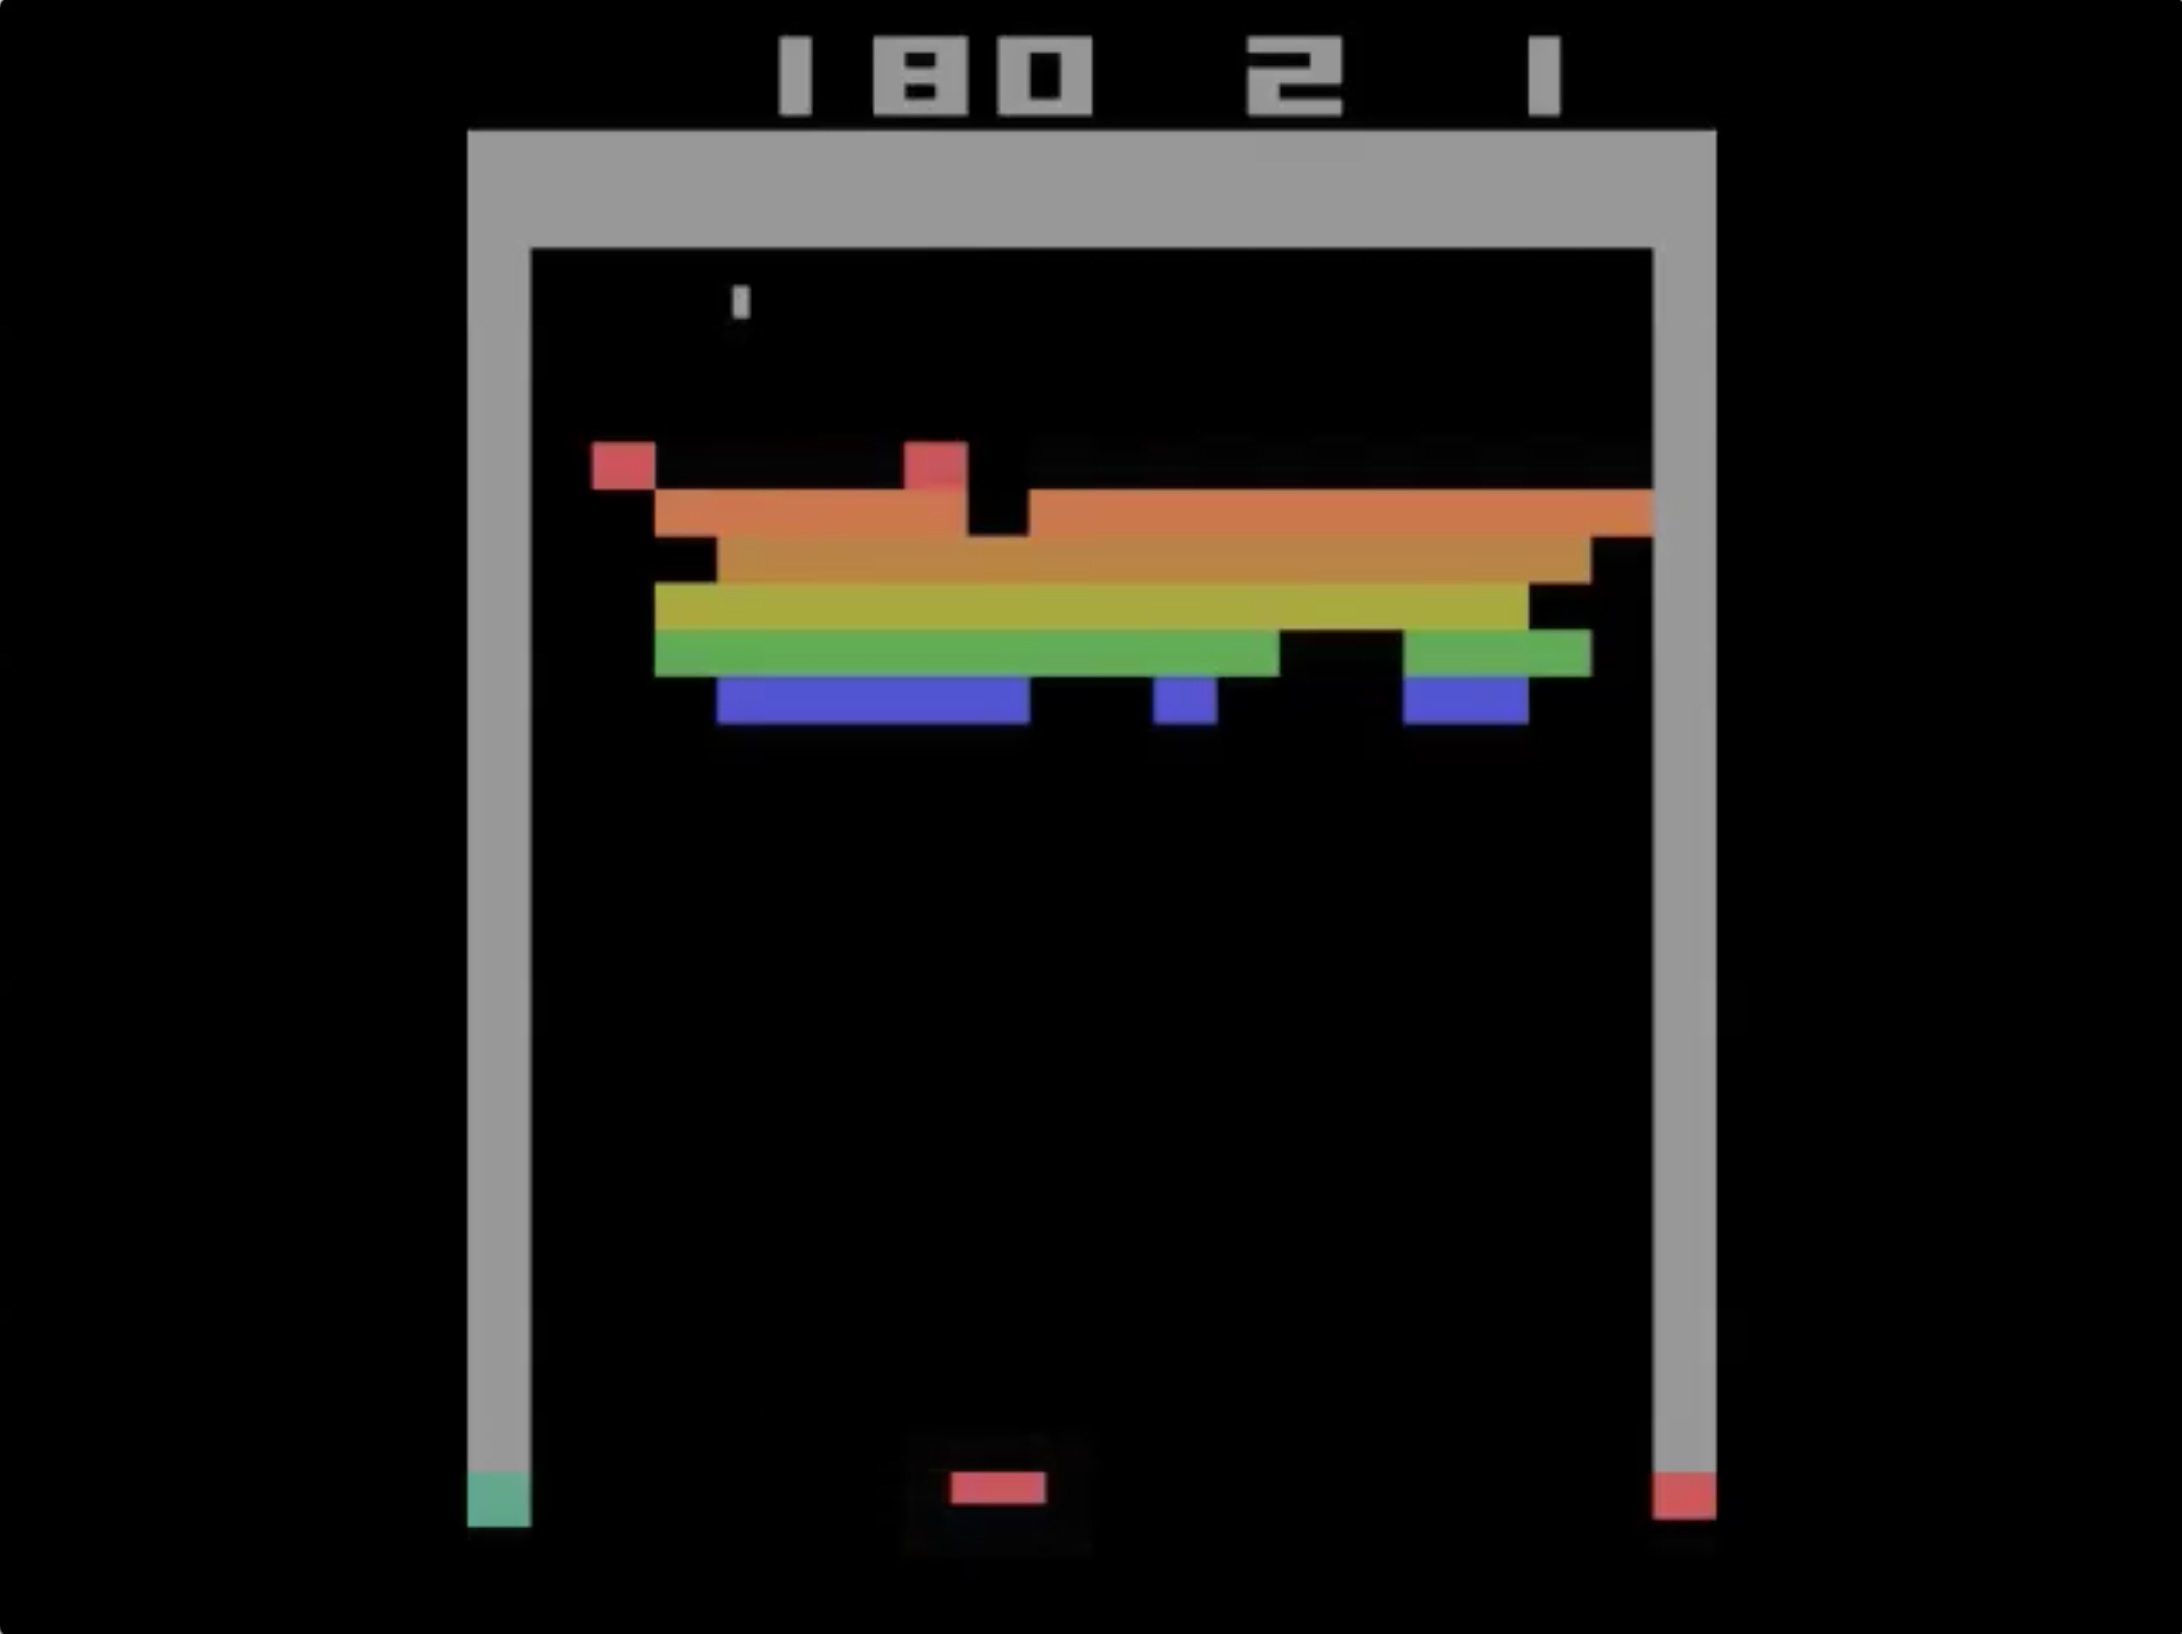
\includegraphics[scale=.065]{img/breakout.jpg}}
  \hspace{1cm}
  \subfigure[Humanoid\label{F:humanoid}]{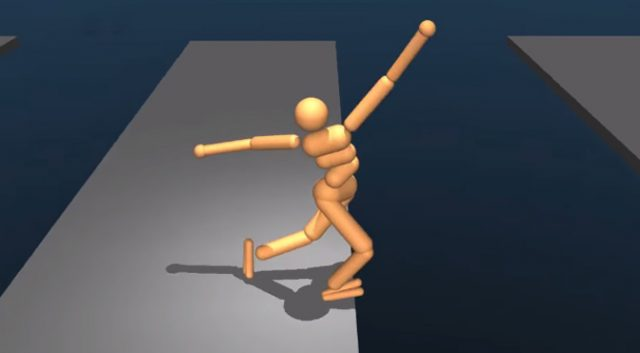
\includegraphics[scale=.3]{img/humanoid.jpg}}
\end{center}
\end{minipage}
\caption[Breakout and Humanoid problems]{Graphical rendering of Breakout and Humanoid problems.}\label{F:breakout_humanoid}
\end{figure}
Considering that the models and their fitting algorithms used in \gls{drl} are the same as those of \gls{dl}, it is intuitive how they can suffer from the previously described issues with an impact on the quality of the learned policy. Figure~\ref{F:breakout_humanoid} shows two examples of environments to highlight problems that may arise when learning how to solve them. In particular, Figure~\ref{F:breakout_frame} refers to the Breakout game briefly described in Section~\ref{S:exploration_drl}. Recalling that in this game the purpose is to catch the ball with the platform on the bottom so as to make it bounce and hit the bricks on the wall at the top, it is intuitive how the number of features needed to solve this games is much less than the whole number of pixels of the raw frame. Thus, hopefully the deep $Q$-network should be able to extract only the few relevant features, such as the coordinates of the ball and the platform, in order to simplify the policy learning. However, this usually does not happen and the network learns a very abstract representation of the input whose semantics is practically not interpretable. On the other hand, Figure~\ref{F:humanoid} refers to a control problem in which a humanoid walker is taught how to walk avoiding obstacles. In this case, the problem lies in the quality of the learned policy to make the humanoid walk. Indeed, usually the policy learned by the agent is effective for solving the environment, but let the humanoid walk in a very unnatural way, very different from the human way of walking.

These examples show that the outcome of the learning process of a \gls{dl} model is almost always very unpredictable and it is unlikely to resemble the model learned by a human being. This happens because is very natural for a human to extract the semantics behind what he/she sees, while for a \gls{dl} model this is generally not a natural way of learning. Taking these considerations into account, I believe that helping \gls{drl} models to extract the real semantics of a problem is a promising way of trying to improve the performance of \gls{drl} algorithms. To this end, the field of Multi-Task learning aims to train a single model on multiple problems. In this way, the knowledge about each task is shared with the one about the other tasks and this helps to force the model in extracting features with significant semantics, just like a regularization method. To this end, I think \gls{drl} is particularly suited thanks to the huge amount of training parameters that may intuitively allow the model to be able to learn multiple problems. Indeed, recently proposed works in \gls{drl} about Multi-Task~\cite{higgins2017darla, ammar2014online, teh2017distral} have shown promising results and I believe that more effort should be put in this direction to make \gls{drl} algorithms more and more efficient.

%\cleardoublepage

\cleardoublepage
\phantomsection
\addcontentsline{toc}{chapter}{\bibname}
\small
\bibliographystyle{plain}
\bibliography{thesis}

\appendix
\chapter{Mushroom}\label{App:msh}
The empirical evaluation of proposed methodologies in \gls{ml} is a critical aspect to take into consideration when publishing a work. Indeed, considering that \gls{ml} is mostly used in practical application, the empirical effectiveness of an algorithm is a desirable property. Because of this reason, the majority of \gls{ml} articles describes a usually extensive empirical section presenting the improvement of the proposed work on the state-of-the-art. This focus on empirical results happens also in \gls{rl} where the algorithms presented in the papers are empirically compared to other methodologies available in literature with the purpose to show some improvements w.r.t. them, e.g. in terms of cumulative discounted reward on several problems.

Several times during my Ph.D. research I needed to implement the code of state-of-the-art algorithms and of the \gls{rl} environments from scratch, since especially at the beginning of my Ph.D. there were not reliable and/or maintained \gls{rl} libraries. Unfortunately, the process of writing codes from scratch for every project was very time consuming and frustrating, especially considering that the same algorithms had to be coded differently just to adapt them to the structure of the ongoing project. Obviously, the problems of time spent in writing code and of reliability of the written code could have been solved with a unified software framework.

For this reason I decided to develop my own \gls{rl} library, which I called \textit{Mushroom}, for helping my research in terms of time and quality. Despite the fact that the development of Mushroom started just for my own purposes, I tried to make it as general as possible and month-by-month it became a general-purpose \gls{rl} library to all effect. Mushroom has the purpose to provide a common interface to develop and run \gls{rl} and it is designed to minimize the effort in writing the code of the experiment: in most cases, the user would only have to write a small script specifying the needed information such as the algorithm to run and the environment. One of the ideas behind Mushroom is to exploit widely used standard libraries such as Pytorch~\cite{paszke2017automatic} and Gym~\cite{gym}, in order to avoid writing new code to implement known algorithms. Mushroom architecture is modular, so that it is possible to include only the needed modules to a system and to implement only the modules that may be needed.

\section{Related works}
Despite the success that \gls{rl} has acquired in the last decade, there are still no standard libraries to perform \gls{rl} experiments. A common interface called RL-Glue~\cite{tanner2009rl} has been proposed in order to allow the communication of agents and environments written in different frameworks and programming languages. However, being only an interface, this library lacks of implementation of \gls{rl} algorithms; furthermore, it is mainly focused on online \gls{rl} algorithms and it is not supported anymore. Nevertheless, a large number of custom libraries are available, but they suffer from heterogeneous drawbacks: poor documentation, lack of algorithms, being very specific for certain tasks or simply no more maintained.

RLPy~\cite{JMLR:v16:geramifard15a} is a good choice to do \gls{rl} experiments with classical algorithms and problems, but currently it does not feature anything related to \gls{drl}; this is an important drawback considering the importance and the ongoing focus of the research on this topic. RLLab~\cite{duan2016benchmarking} is a more modern alternative to RLPy and a good choice for researchers focusing on continuous \gls{drl}. Other recent libraries mostly focused on \gls{drl} However, this library does not cover classical \gls{rl} methodologies and this results in a library useful only for a limited number of researchers. More recent \gls{drl} libraries are TensorForce~\cite{schaarschmidt2017tensorforce} and ChainerRL~\cite{bworld}, that are \gls{rl} extensions of deep learning libraries.

Eventually, there are many libraries featuring a single algorithm. For instance, simple-dqn~\cite{simpledqn} implements the \gls{dqn} algorithm giving the possibility to replicate the experiments in~\cite{mnih2015human} and the low complexity of the code allows to significantly customize it. Of course, the usefulness of such a library is limited to projects related to \gls{dqn}.

\section{Ideas and Concepts}
Mushroom is an easily accessible, yet powerful, \gls{rl} library useful for research and didactic purposes.
\paragraph{General purpose} Mushroom adapts to heterogeneous learning tasks based on the interaction of an agent with an environment. This is achieved by a common interface shared by different algorithms, even suitable for different problems: batch and online algorithms, episodic and infinite horizon tasks, on-policy and off-policy learning, and many others.
\paragraph{Lightweight}
Mushroom is both user-friendly and flexible: only a high-level interface is exposed to the user, hiding low-level aspects. For instance, the user should not care about the implementation details to use a function regressor for different tasks, since they are hidden by a simple common interface. However, we leave the check of consistency constraints to the user, e.g. avoiding the use of a tabular algorithm for an environment with continuous state space. Minimal interfaces simplify the implementation of new algorithms, as there are no hard constraints in the prototypes.
\paragraph{Compatible}
Standard Python libraries useful for \gls{rl} tasks have been adopted:
\begin{itemize}
 \item \textit{Scientific calculus}: numpy, scipy;
 \item \textit{Basic \gls{ml}}: scikit-learn;
 \item \textit{\gls{rl} benchmark}: gym;
 \item \textit{Neural networks and \gls{gpu} computation}: pytorch, tensorflow, theano;
 \item \textit{Plotting}: matplotlib.
\end{itemize}
Mushroom provides an interface to these libraries, in order to integrate their functionalities in the framework, e.g. an interface for gym environments, support for regression with scikit-learn models.

\paragraph{Easy to use}
Mushroom enables to develop and run experiments writing a minimal amount of code. In most of the tasks an experiment can be written in a few Python lines without the need of complex configuration files. The majority of the \gls{rl} problems can be solved with experiments written following the structure of the library examples.

\section{Design}
The main module of Mushroom is the \texttt{Core} whose purpose is to manage the interaction between the agent and the environment for both learning and testing tasks.
The common interface \texttt{Environment}, extended by each problem implementation, contains the main properties of the environment: discount factor, horizon (i.e. maximum episode length), observation and action spaces.
Each learning algorithm must extend the \texttt{Agent} class which also provides a common interface to interact with the environment following a specified policy, e.g. a $\varepsilon$-greedy policy.
An instance of the \texttt{Core} class is built providing an agent and an environment object. It defines the \texttt{learn} and the \texttt{evaluate} methods, which implement the interaction of the agent on the environment.

The \texttt{evaluate} method runs the current policy on the environment and collects the dataset. The \texttt{learn} method also feeds the collected dataset to the learning algorithm of the agent, when needed. Both these methods can be run for a fixed number of episodes or steps; moreover, \texttt{learn} allows to specify the frequency, in terms of episodes or steps, of the call to the learning algorithm. Thanks to this choice, it is possible to implement online and batch algorithms transparently. The \texttt{Core} can also run a list of callback functions after each learning step.
\begin{python}
# Online learning running for $30$ episodes
core.learn(n_steps=30, n_steps_per_fit=1)
# Batch learning over a dataset of 30 episodes
core.learn(n_episodes=30, n_episodes_per_fit=30)
# Online learning for 300 episodes, learning every 50 step
core.learn(n_episodes=300, n_steps_per_fit=50)
\end{python}
\begin{figure}[t]
\centering
 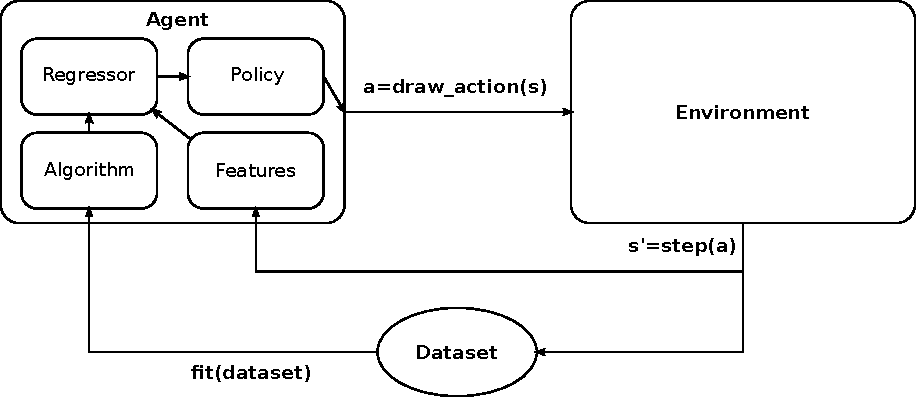
\includegraphics[width=.8\textwidth]{img/msh.pdf}
 \caption{Interaction between the agent and the environment when the \texttt{learn} method of the \texttt{Core} class is called. A dataset, collected during this interaction, is used to update the approximator (e.g. policy, $Q$-function).}
\end{figure}\label{F:core}

To simplify the implementation of generic \gls{rl} algorithms, and \gls{td} algorithms in particular, Mushroom offers a high-level interface for the function regressors. This interface supports the use of ensemble regressors that are created specifying the number of models in the ensemble. Moreover, it manages the regressor of the $Q$-function in the case of discrete action spaces: it transparently deals with the creation of a different regressor for each action or a single regressor with a different output for each action. The user should not care about the low-level implementation of these regressors, since everything is managed by the \texttt{Regressor} interface, which also supports generic function approximator. Furthermore, both parametric and non-parametric are transparently managed by the interface.
\begin{python}
# $Q$-function regressor with $5$ different linear approximator
approximator = Regressor(LinearApproximator, n_actions=5, output_shape=(1,), ...)
# $Q$-function regressor with a single linear approximator with 5 outputs
approximator = Regressor(LinearApproximator, n_actions=5, output_shape=(5,), ...)
# Generic linear approximator
approximator = Regressor(LinearApproximator, output_shape=(1,), ...)
\end{python}
The same logic used to implement the \texttt{Regressor} interface, has been used in the \texttt{Features} interface that has the purpose to transparently manage a generic set of basis functions, sparse features (e.g. tiles) and \gls{gpu}-accelerated basis functions implemented with Pytorch~\cite{paszke2017automatic}.


\end{document}
